\documentclass[fleqn]{report}
\usepackage{fullpage}
\usepackage{fancyhdr}
\usepackage{amsmath}
\usepackage{amssymb}
\usepackage{bm}
\usepackage{hyperref} 
\usepackage{underscore} %This is messy - it means no underscores in labels or figure names.
\usepackage{subfigure}
\usepackage{fancyvrb}
\usepackage{chngpage} % allows for temporary adjustment of side margins
\usepackage{lscape} % allows for some landscape orientated pages, the pdf version is:
\usepackage{cancel}
%\usepackage{pdflscape}

% \usepackage[small,compact]{titlesec}

% Comment this as well as the \printindex at the end out to avoid the generation of a 
% book index 
% \usepackage{makeidx}
% \makeindex 
% To simplify the build, do not generate the index
\renewcommand{\index}[1]{}

\usepackage{nomencl} % List of symbols 
\makenomenclature


%Comment the block below to remove the version control footers.  Leave the definitions in each chapter file alone!.
\pagestyle{fancy}
\fancyhead{} %leave this here to blank fancy header
\renewcommand{\headrulewidth}{0pt} %leave this here to blank header line
\fancyfoot[C]{$\qquad \qquad \qquad \qquad \qquad \qquad \qquad \qquad$ \thepage} %To avoid clash with date

% The convention is British spelling:
%  -ise -isation, like in 'parallelise', 
%  centre
%  analyse
%  analogue

\hypersetup{
bookmarks,
plainpages=false,
colorlinks=true,
pdfborder={0 0 0 0},
linkcolor=blue,
citecolor=blue,
urlcolor=blue,
pdfstartview={FitH},
pdftitle={GKW Manual},
bookmarksopen=false,
unicode
}
%if not using hyperref, uncomment this
%\newcommand\texorpdfstring[2]{#1}

%Attempt to keep the complete set of equations on one page...
\setlength{\textheight}{24cm}
%\setlength{\textwidth}{16cm}
%\topskip{21mm}
%\bottomskip{21mm}
\setlength{\topmargin}{-10truemm}
%\setlength{\abovedisplayskip}{10pt}
%\setlength{\belowdisplayskip}{10pt}


%For Binding
%\setlength{\oddsidemargin}{+10truemm}
%\setlength{\evensidemargin}{-10truemm}

%Double Spacing
%\renewcommand{\baselinestretch}{2}
%\parindent0cm

%Controlling Floats
%\renewcommand{\textfraction}{0.15}
%\renewcommand{\topfraction}{0.85}
%\renewcommand{\bottomfraction}{0.85}
%\renewcommand{\floatpagefraction}{0.9}

% define an environment to escape underscores (not needed in href environments due to underscaore package)
% this is a neater alternative
\makeatletter
\DeclareRobustCommand*{\escapeus}[1]{%
  \begingroup\@activeus\scantokens{#1\endinput}\endgroup}
\begingroup\lccode`\~=`\_\relax
   \lowercase{\endgroup\def\@activeus{\catcode`\_=\active \let~\_}}
\makeatother

%% Various macros are defined below in order to aid with the formatting
%% and to enable indexing at some point (via makeindex, xindy or similar).
%% Please use these and add more as appropriate.

\usepackage{gkwdoccommands}

\setlength{\mathindent}{0.5cm}

\usepackage{graphicx}
\graphicspath{{../fig/}}


\begin{document}

\title{GKW how and why}

\author{A.G. Peeters, R. Buchholz, Y. Camenen, F.J. Casson, \\ 
        S. Grosshauser, W.A. Hornsby, P. Manas, P. Migliano, \\
        M. Siccinio, A.P. Snodin, D. Strintzi, T. Sung, \\ 
        G. Szepesi, D. Zarzoso}  

\date{Updated in 2016, work in progress. \thanks{Copyright \copyright{}
2007-2016, by named authors.}}

\maketitle

\setlength{\parskip}{8pt}
\setlength{\parindent}{0pt}

\chapter*{Preface}

This documentation comes with the GKW code. It is largely based on our 2009 paper in Computer Physics Communications Ref. \cite{CPC-paper},
but contains additional material and descriptions of additional features that the code has aquired since that paper.
In this manual GKW is presented 
with the aim of documenting the exact equations solved, presenting the essential benchmarks which 
document the proper numerical solution, and explaining the code structure and installation.  
This document is evolving along with the code, and 
currency and completeness presently take precedence over integration and polish of all sections.  
GKW developers are strongly urged to update this document (\doc{tex/doc.tex}) to reflect changes made in the code repository.


\section*{What is GKW?}

Gyrokinetic Workshop (GKW) is a code for the simulation of microinstabilities and turbulence in a magnetically confined plasma.
%The code incorporates all physics effects that can be expected from a state of the art gyrokinetic simulation code in the 
%local limit: kinetic electrons, electromagnetic effects, collisions, full general geometry with a coupling to a MHD equilibrium code, 
%and ExB shearing.
%In addition the physics of plasma rotation has been implemented through a formulation of the gyrokinetic equation in the co-moving %system. 
The gyrokinetic model is is five dimensional partial differential equation and its solution requires a massively parallel approach. 
GKW is written in Fortran 95 and has been parallelised using MPI, which enables it to scale well up to 32768+ cores.
The code was initially developed at the University of Warwick in 2007 through the extension of the linear code
LINART \cite{PEE04}, and can be used both in the linear as well as in the nonlinear regime. In 2016 it has been renamed from 'Gyrokinetics at Warwick' to 'Gyrokinetic Workshop', to reflect the nonlocality of its developers and users.
The code has been freely available online since 2010,
and has been hosted at \href{https://bitbucket.org/gkw/gkw}{https://bitbucket.org/gkw/gkw},
since 2015, where it is actively maintained.

\section*{Can I use GKW?}

You can obtain and use GKW for any purpose with minimal restrictions.
Essentially you can make any changes to the source, and are not obliged to inform us or communicate 
these changes back to us (although we would welcome it if you did).  
Furthermore, you are free to redistribute the code to others under the terms of the
license (see the LICENSE file), which is the GNU General Public License version 3.

We politely request that the effort made by us is recognised. 
In any publication that uses the results of GKW, either directly or indirectly,
you should cite the CPC paper \cite{CPC-paper}. (If you want to be kind to us you could additionally
cite the original LINART paper Ref. \cite{PEE04} and/or the first paper in which GKW has been
used Ref. \cite{PEE07}).

%N.B. This section only works because of the present document style and the ordering of the references above.
\subsection*{References}

\begin{enumerate}
\item A.G. Peeters, Y. Camenen, F.J. Casson, W.A. Hornsby, A.P. Snodin, D. Strintzi, G. Szepesi,\\
Computer Physics Communications, {\bf 180}, \href{http://dx.doi.org/10.1016/j.cpc.2009.07.001}{2650}, (2009)
\item A.G. Peeters, D. Strintzi, Phys. Plasmas {\bf 11},  \href{http://dx.doi.org/10.1063/1.1762876}{3748}, (2004)
\item A.G. Peeters, C. Angioni, D. Strintzi, Phys. Rev. Lett. {\bf 98},  \href{http://dx.doi.org/10.1103/PhysRevLett.98.265003}{265003}, (2007)
\end{enumerate}

\pagebreak


\section*{What does GKW do?}

GKW aims at solving the turbulent transport problem arising in tokamak plasmas. It solves
the gyrokinetic (the kinetic Vlasov equation averaged over the fast gyro-motion) equation on a fixed
grid in the 5-dimensional space using a combination of finite difference and pseudo spectral
methods. The solution of the kinetic equations governing this problem is an active area of 
research, with many groups worldwide contributing. The two approaches used are Particle in Cell 
(PIC) codes \cite{PAR93,LIN98,IDO03,HEI04,BOT07,JOL07,GRA06}, and Vlasov codes 
\cite{KOT95,DOR00,JEN00,DAN05,CAN03}. GKW obviously falls in the latter category, and 
reaches a standard that can be expected from a modern Vlasov code, i.e. it includes kinetic 
electrons, a general description of the geometry with a coupling to a MHD equilibrium solver, 
electro-magnetic effects, collisions, and the effect of ExB shearing. In addition the physics of 
toroidal plasma rotation is included through a formulation of the equations in the co-moving system.   
The physics of rotation is currently an active area of research and many of the applications of 
GKW have concentrated on the transport of toroidal momentum \cite{PEE07,PEE05,PEE06,
PEE09com,PEE09,CAM09,PEE09scmode,CAM09pop,CAS09}, the influence of rotation on 
other transport channels \cite{CAM09rot,CAS10}, and the interaction between turbulence and islands \cite{HOR10,HOR10epl}.
% Update the references above

\section*{Code summary}

{\bf Licensing provisions:} GNU GPLv3

{\bf Programming language:} Fortran 95

{\bf RAM:} $\sim$~128MB-1GB for a linear run; 25GB for typical nonlinear kinetic run (30 million grid points).

{\bf Number of processors used:} 1, although the program can efficiently utilise 4096+ processors (spectral), depending on problem and available computer. 128 processors is reasonable for a typical nonlinear kinetic run on the latest x86-64 machines.  The nonspectral scheme can efficiently scale to 32768+ processors.

{\bf External routines/libraries:}  None required, although the functionality of the program is somewhat
limited without a MPI implementation (preferably MPI-2) and the FFTW3 library.  In addition, the nonspectral and
implicit schemes require the UMFPACK and AMD libraries, and the eigenvalue solver requires the SLEPc and PETSc libraries. Furthermore, GKW can be compiled to support the HDF5 output format.

{\bf Standard solution method:} Pseudo-spectral and finite difference with explicit time integration.

{\bf Running time:} (On recent x86-64 hardware) $\sim$5 minutes for a short linear problem; 4000
hours for typical nonlinear kinetic run.

{\bf Geometry Interface:}  The MHD equilibrium code CHEASE \cite{LUT96} is used for the general geometry calculations. This code has been developed in CRPP Lausanne and
is not distributed together with GKW, but can be downloaded separately. The geometry module of GKW is based on the version 7.3 of CHEASE, which includes the output for Hamada coordinates.\\

\setlength{\parskip}{0pt}
\setlength{\parindent}{0pt}

\tableofcontents

\setlength{\parskip}{8pt}
\setlength{\parindent}{0pt}

\newpage
 

% related to auctex mode and latex-preview-mode in Emacs:
%%% Local Variables:
%%% mode: latex
%%% TeX-master: "doc"
%%% End:

\chapter{Gyrokinetic theory}

\section{The gyrokinetic framework}
\label{sec:framework}
The starting point of the equation for the evolution of the distribution function is the 
gyrokinetic theory formulated in Refs \cite{LIT83,HAH88,BRI88,SUG00}. In GKW these equations 
are solved up to first order in the Larmor radius over the major radius $\rho_* \ll 1 $ 
(with the exception of the polarisation which enters in the field equations). 
In order to determine which of the terms in the original formulation of the theory (which is
accurate up to second order in $\rho_*$) must be kept, we will here briefly discuss the ordering. 
More details can be found in Ref.~\cite{PEE09}.

A thermal velocity ($v_{\rm th}$) and a major radius ($R$) are used to normalise the length and 
time scales. For the gradients we assume 
\begin{equation} 
R \nabla_\parallel  \approx 1 \qquad 
R \nabla_\perp \approx 1/ \rho_*,
\end{equation} 
i.e. the solution is assumed to have a length scale of the order of the system size along the 
field, but can have a length scale of the order of the Larmor radius perpendicular to the 
magnetic field. 
This difference in length scales means that the convecting velocities must be evaluated to a 
different order parallel and perpendicular to the field. 
The velocity along the field is to be evaluated in lowest order only (i.e. of the order of $v_{\rm th}$), but
the perpendicular velocity must be evaluated up to first order (order $\rho_* v_{\rm th}$). 
In GKW the perturbations in the electro-static potential $\phi$ as well as the vector potential ${\bf A}$ are 
retained.
For the latter it is, however, assumed that 
\begin{equation} 
{\bf A} = A_\parallel {\bf b} ,
\end{equation}
where ${\bf b}$ is the unit vector in the direction of the unperturbed magnetic field. 
The assumption above means that no compressional effects of the magnetic field are retained in the 
description.
Compressional effects are currently implemented in the code but are not yet described here.  
Note that the vector potential above is the perturbed vector potential not to be confused with the one 
connected with the equilibrium magnetic field.
The equations will be formulated in the co-moving system of a toroidally rotating plasma. 
The $E \times B$ drift velocity connected with this toroidal rotation is of the order of the thermal 
velocity in the laboratory frame, but the transformation to the co-moving frame removes this largest order $E \times B$ velocity from the 
equations \cite{PEE09,Casson-Thesis}. The transformation to the co-moving frame also introduces a background centrifugal potential $\Phi$.
The perturbed potential $\phi$, perturbed vector potential $A_\parallel$, and background potential $\Phi$
in the co-moving frame can then be taken to be of the order 
\begin{equation} 
\phi \approx {T \over e} \rho_* \qquad 
A_\parallel \approx {T \over e v_{\rm th}} \rho_*
\qquad
\Phi \approx {T \over e} \qquad 
\label{fieldordering}
\end{equation}
where $T$ is the temperature, and $e$ is the elementary charge. 
Since $\Phi$ is an equilibrium quantity, the length scale of any variation is assumed large compared
to the Larmor radius, whilst the perturbed quantities may have perpendicular gradient length scales on the order of the Larmor radius.  
The field gradients can then be shown to be of the same order, with $\nabla_\perp \phi \approx \nabla_\perp \Phi$.  
From these assumptions it can be derived that the $E \times B$ velocity is of the order $\rho_* v_{\rm th}$. 

Gyro-centre coordinates (${\bf X},\mu,v_\parallel$) are used, with ${\bf X}$ being the gyro-centre position, $v_\parallel$ the parallel (to the magnetic field) velocity, and $\mu$ the magnetic moment $\mu = {m v_\perp^2 / 2 B} $.  
Here $v_\perp$ is the velocity component perpendicular to the equilibrium magnetic field ${\bf B}$, $m$
is the particle mass and $B$ is the magnetic field strength. 
The magnetic moment is an invariant of motion, but the parallel velocity changes due to the electric field 
acceleration and mirror force. 
It turns out that for consistency one needs to keep both the lowest as well as the first order (in $\rho_*$) 
contribution to the acceleration. 

%FJC -> GSZ Add Bpar ordering here?

Finally, the approximation known as the $\delta f$ approximation is employed. 
This approximation assumes that the perturbed distribution $f$ is much smaller than the background distribution 
$F$, but has a perpendicular length scale of the order of the Larmor radius whereas the background varies 
on the length scale of the system size:
\begin{equation} 
f \approx \rho_* F \qquad 
{\partial f \over \partial v_\parallel} \approx \rho_* {\partial F \over \partial v_\parallel}  \qquad 
\nabla f \approx \nabla F .
\end{equation}
The ordering assumption above removes the `velocity non-linearity' (combinations of the 
electro-magnetic fields and the velocity space derivative of the perturbed distribution) from
the evolution equation of the perturbed distribution. 
The disadvantage is  that strict energy conservation no longer applies.   

With the help of these approximations the gyrokinetic equation of Refs. \cite{LIT83,BRI88,SUG00}
can be rewritten. 

\section{Lagrangian}
\label{sec:theoryLagrangian}
(This section is not in the CPC paper which instead refers to Ref. \cite{PEE09} which contains the full derivation with centrifugal effects.)
(CHECK CONSISTENCY)

The starting point is the Lagrangian \index{Lagrangian}
\begin{equation}
  \gamma=\left({e\over c}{\bf A}+{e\over c}A_{\parallel}{\bf b}+m{\bf v} \right)\cdot d{\bf x}-\left({m\over 2}v^{2}+e\phi \right)dt
\end{equation}
The coordinates are transformed into guiding center coordinates. The electrostatic guiding center
Lagrangian is known, and can be found in Hahm 1988 \cite{HAH88}. For the magnetic perturbations we take that
\begin{equation}
  A_{\parallel}({\bf X}+{\bf \rho}){\bf b} \cdot d({\bf X}+\rho)
\end{equation}
where $\rho =\rho({\bf X},{\mu},{\theta})$. All the derivatives of $\rho$ will give vectors
perpendicular to the magnetic field. Thus if there is not a perpendicular magnetic potential
perturbation, the only term that survives is
$$A_{\parallel}{\bf b}\cdot d{\bf X}$$
Then the guiding center Lagrangian is
\begin{equation}
\gamma =\left({e\over c}{\bf A}+{e\over c}A_{\parallel}{\bf b}+mv_{\parallel}{\bf b} \right)\cdot 
d{\bf X}+\mu d\theta -\left({m\over 2}v_{\parallel}^{2}+\mu B+e\phi \right)dt
\end{equation}
This Lagrangian is transformed in the gyrocenter coordinates with the Lie transforms.
To the first order, if there are no perpendicular perturbations in the magnetic potential,
we can just substitute the perturbations of the fields with the respective gyroaveraged quantities. 
This can also be derived rigorously with the Lie transforms. The new Lagrangian will be
\begin{equation}
\Gamma =\left({e\over c}{\bf A}+{e\over c}\ga{A_{\parallel}}{\bf b}+mv_{\parallel}{\bf b} \right)\cdot 
d{\bf X}+\mu d\theta -\left({m\over 2}v_{\parallel}^{2}+\mu B+e\ga{\phi} \right)dt
\label{eq:gyrocenterlagrangian}
\end{equation}
where now ${\bf X},\mu,v_{\parallel},\theta$ are the gyrocenter coordinates. From this one can derive 
the equations of motion using the Euler Lagrange equations
\begin{equation}
\omega_{ij}{dz^{j}\over dt}={\partial H \over \partial z^{i}}-{\partial \gamma_{i}\over \partial t}
\end{equation}
FIXME what is $\mathrm{d}\gamma$ or $\partial\gamma$ supposed to mean if $\gamma$ is already a differential (cf. \eqref{eq:gyrocenterlagrangian})?
where $H$ is the Hamiltonian and 
\begin{equation}
\omega_{ij}={\partial \gamma_{j}\over \partial z^{i}}-{\partial \gamma_{i}\over \partial z^{j}}
\end{equation}
are the Lagrange brackets.

The Lagrange brackets that are of interest are
\begin{equation}
\omega_{X_{i}X_{j}}={e\over c}\epsilon_{ijk}{\hat B}_{k}
\end{equation}
\begin{equation}
\omega_{{\bf X}U}=-m{\bf b}
\end{equation}
where 
\begin{equation}
{\hat {\bf B}}=\nabla \times {\bf A}+\nabla \times A_{\parallel}{\bf b}+{mc \over e}v_{\parallel}\nabla \times {\bf b}
\end{equation}

Choosing $i=U$ we get that
\begin{equation}
m{\bf b}\cdot {\dot {\bf X}}=mv_{\parallel}
\end{equation}
Choosing $i={\bf X}$ we get that
\begin{equation}
m{\dot v}_{\parallel}{\bf b}-{e\over c}{\dot {\bf X}}\times {\hat{\bf B}}=-e\nabla \ga{\phi}-\mu \nabla B-{e\over c}
{\partial \ga{A_{\parallel}}\over \partial t}{\bf b}
\end{equation}
and taking that
\begin{equation}
{\bf E}=-\nabla \phi -{1\over c}{\partial \ga{A_{\parallel}}\over \partial t}{\bf b}
\end{equation}
we get that
\begin{equation}
m{\dot v}_{\parallel}{\bf b}-{e\over c}{\dot {\bf X}}\times {\hat{\bf B}}=e{\bf E}-\mu \nabla B
\end{equation}

We can cross this equation with ${\bf b}$ to derive the equation for $\dot X$. To derive the equation of GKW we have
to approximate
\begin{equation}
\nabla \times \ga{ A_\parallel} {\bf b}
= 
\nabla \ga{A_\parallel}\times\mathbf{b} + \ga{A_\parallel}\nabla\times\mathbf{b}
 \approx - {\bf b} \times \nabla \langle A_\parallel \rangle 
\label{eq:approxtofindExBdrift}
\end{equation}
Then the equation of $\dot X$ is.
\begin{equation} 
{{\rm d} {\bf X} \over {\rm d} t} = v_\parallel {\bf b} + {\bf v}_D + {\bf v}_E + {\bf v}_{\delta B_\perp}, 
\end{equation}
To derive the equation for $v_{\parallel}$ we dot with $\dot X$. This gives
\begin{equation}
mv_{\parallel}{\dot v}_{\parallel}={\dot {\bf X}}\cdot \left(e{\bf E}-\mu \nabla B\right)
\end{equation}

\section{The gyrokinetic equation}

In a rigidly rotating frame, 
the evolution of equation for the gyro-centre position ${\bf X}$, and the parallel velocity are \cite{PEE09}
\begin{equation} 
{{\rm d} {\bf X} \over {\rm d} t} = v_\parallel {\bf b} + {\bf v}_D + {\bf v}_\chi ,
\qquad
\label{eq:drifts}
%\end{equation}
%\begin{equation} 
m v_\parallel {{\rm d} v_\parallel \over {\rm d} t} =   
{{\rm d} {\bf X} \over {\rm d} t} \cdot \left[ Z {e }{\bf E}  - \mu 
 \nabla B + m\Omega^2 R \nabla R \right],
%\end{equation}
%where $\mu$ is a constant of motion. 
%\begin{equation} 
\qquad 
{{\rm d} \mu \over {\rm d} t} = 0 .
\end{equation}
Here $Z$ is the particle charge, $R$ the local major radius, and $\Omega$ the frame rotation frequency.  
$\bf E$ is the gyro-averaged perturbed electric field plus the inertial electric field
\begin{equation} 
{\bf E} = -\nabla \langle \phi \rangle  - {\partial \langle A_\parallel \rangle \over \partial t} {\bf b}  -\nabla \langle \Phi \rangle ,
\end{equation}
where the angle brackets denote the gyro-average. 
Since $\Phi$ is an equilibrium quantity, the scale lengths of any variation are assumed large compared
to the Larmor radius and we neglect the gyroaverage, taking $\Phi \approx \langle\Phi\rangle$.  (The 
full details of the calculation of $\Phi$ are given in Sec. \ref{cfphi}).  

The velocities in \eq{drifts} are from left to right: the parallel motion along the 
unperturbed field ($v_\parallel {\bf b}$), the drift motion due to the inhomogeneous field 
(${\bf v}_D$), and 
\begin{equation} 
\label{eq:v-chi}
{\bf v}_\chi = {{\bf b} \times \nabla \chi \over B} \qquad 
\textrm{with} \qquad \chi = \langle \phi \rangle - v_\parallel \langle A_\parallel \rangle ,
\end{equation}
which is the combination of the $E \times B$ velocity 
(${\bf v}_E = {\bf b} \times \nabla \langle \phi \rangle / B$) and the parallel motion along 
the perturbed field line (${\bf v}_{\delta B} = - {{\bf b} \times \nabla v_\parallel 
\langle A_\parallel \rangle /B}$).
The drifts due to the inhomogeneous magnetic field and inertial terms can be written in the form
\begin{equation}
\label{eq:driftsinhomogeneousinterial}
{\bf v}_D = 
{1\over Ze} \biggl [ {m v_\parallel^2\over B} + \mu \biggr ] {{\bf B} \times \nabla B \over B^2}  
+ {m v_\parallel^2 \over 2 Z e B} \beta^\prime {\bf b} \times \nabla \psi
+ { 2 m v_\parallel \over Z e B } {\bf \Omega}_\perp + {1 \over ZeB} {\bf b} \times \nabla \cfen
\end{equation}
In the equation above $\psi$ is a radial coordinate (flux label) and ${\bf \Omega}_\perp$ is the angular
(toroidal) rotation vector perpendicular to the field, i.e. ${\bf \Omega}_\perp = {\bf \Omega} 
- ({\bf \Omega } \cdot {\bf b}) {\bf b}$.
The first term on the right is the combination of the grad-B drift and curvature drift 
in the low beta approximation, whereas the second term, involving
\begin{equation}
\label{eq:defbetapr}
\beta' = \frac{2\mu_0}{B^2}\frac{\partial p}{\partial \psi},
\end{equation}
is the correction to the 
curvature drift due to the modification of the equilibrium associated with the pressure
gradient. The penultimate term is the Coriolis drift derived in Ref.~\cite{PEE07} 
using the formulation of the gyrokinetic equations in the co-moving frame \cite{BRI95}.
The formulation of Ref.~\cite{PEE07} was extended in Refs.~\cite{PEE09,Casson-Thesis} to include 
the centrifugal force, and the first centrifugal results were published in  Refs.~\cite{CAS10,Casson-Thesis}.  
The last term combines the centrifugal drift and background potential 
in the (species dependent) centrifugal energy
\begin{equation}
\cfen=Ze\Phi - {1 \over 2} m \Omega^2 (R^2-R_0^2)
\end{equation}
where $R_0$ is the major radius of the point on the flux surface at which the densities are defined.

From the equations above the gyrokinetic equation in (${\bf X}, v_\parallel, 
\mu$) coordinates can be derived: \cite{LIT83,PEE09}
\begin{equation} 
{\partial f_{\rm tot} \over \partial t} + {{\rm d} {\bf X} \over {\rm d} t} \cdot \nabla_\mu 
f_{\rm tot} + {{\rm d} v_\parallel \over {\rm d} t} {\partial f_{\rm tot} \over \partial v_\parallel} = 0 .
\end{equation} 
The distribution function $f_{\rm tot}$ in this equation is split in a background $F$ and a perturbed 
distribution $f$. As discussed in Section \ref{sec:framework} the $\delta f$ approximation 
will be employed. 
Consequently, the equation for $f$ can be written in the form \cite{PEE09}
\begin{equation} 
{\partial f \over \partial t} + (v_\parallel {\bf b} + {\bf v}_D + {\bf v}_\chi) \cdot \nabla f  
-{{\bf b} \over m}\cdot(\mu \nabla B + \nabla \cfen){\partial f \over \partial v_\parallel} = S. 
\end{equation}
where $S$ is determined by the background distribution function.
The latter is assumed to be a Maxwellian ($F_M$), with
temperature ($T$) and mean parallel velocity ($u_\parallel$) being functions of the radial coordinate only.
In the case of a rotating plasma the density in the flux surface varies as $n(\theta)=n_{R_0} \exp(-\cfen(\theta)/T)$
and is kept in the solution of the equilibrium equation \cite{PEE09}.
\begin{equation} 
\label{eq:maxwell}
F_M = {n_{R_0} \over \pi^{3/2} v_{\rm th}^3 } \exp 
\biggl [ - {(v_\parallel-(R B_t/B)\omega_\phi )^2 + 2 \mu B / m \over v_{\rm th}^2} - \cfen/T \biggr ] . 
\end{equation} 
Here $v_{\rm th}\equiv \sqrt{ 2 T / m}$ is the thermal velocity (note that in this area of 
research the thermal velocity is usually defined without the $\sqrt{2}$ factor).
The appearance of an explicit rotation velocity $u_\parallel$ in the Maxwellian may be confusing since the equations are formulated
in the co-moving system in which the rotation vanishes. 
However, under experimental conditions the plasma rotation $\omega(\phi)$ has a radial gradient while the frame is chosen
to rotate as a rigid body with a constant angular frequency $\Omega$. 
Indeed a differential rotation of the frame would be impractical since the distance between two
fixed points in the co-moving 
system would increase in time, i.e. the metric would be time dependent. 

The local model constructed here chooses the rotation of the frame to be equal to the plasma rotation at one particular radius. 
Therefore $\omega_\phi$ in the above Maxwellian is zero at the radial location considered, but has a finite radial gradient. This 
gradient will enter the equations as $\nabla \omega_\phi$. (for more details see Ref.~\cite{PEE09}).  

The term containing the derivative of the vector potential towards time presents a numerical difficulty. 
In the $\delta f$ formalism it can, however, easily be combined with the time derivative of $f$. If one defines a `new' distribution $g$ 
\begin{equation} 
g = f + {Z e \over T} v_\parallel \langle A_\parallel \rangle F_M ,
\end{equation}
and replaces the time derivative of $f$ in the gyrokinetic equation with the time derivative of $g$, the cumbersome 
time derivative of $\langle A_\parallel \rangle $ is removed. 
Using the equations above one arrives at the following equation for the distribution function $g$
\begin{equation} 
{\partial g \over \partial t} + {\bf v}_\chi \cdot \nabla g  + (v_\parallel {\bf b} + {\bf v}_D) \cdot \nabla f  
-{{\bf b} \over m}\cdot(\mu \nabla B + \nabla \cfen){\partial f \over \partial v_\parallel} = S. 
\label{Vlasov}
\end{equation}
where $S$ is given by
\begin{equation}
S =  - ({\bf v}_\chi + {\bf v}_D) \cdot \biggl [ {\nabla n_{R_0} \over n_{R_0}} + \biggl ( {v_\parallel^2 \over v_{\rm th}^2 } 
+ {(\mu B + \cfen) \over T} - {3 \over 2} \biggr ) {\nabla T \over T} + {m v_\parallel \over T} {R B_t \over B }\nabla \omega_\phi \biggr ] F_M -  
{Ze \over T} [ v_\parallel {\bf b} + {\bf v}_D ] \cdot \nabla \langle \phi \rangle  F_M .
\label{source} 
\end{equation}
Note that both $g$ and $f$ appear in this equation. Since any form of dissipation on the field variables 
leads to a numerical instability \cite{CAN03}, it is preferable to use $f$ in any term that requires 
dissipation for stable numerical implementation.  
It should also be noted here that the Maxwellian is not an exact solution of the gyrokinetic equation in the limit of a zero 
perturbed electro-magnetic field. 
From the equation above it follows that $S$ is nonzero due to the drifts connected with the magnetic field inhomogeneity 
in the gradients of density temperature and velocity. 
The solution of the evolution equation will determine the deviation away from the Maxwellian as a nonzero perturbed
distribution $f$. 
This perturbation is of the order $\rho_* F_M$, and neglecting it as part of the background distribution is consistent with 
the ordering adopted. 
The drift term is ${\bf v}_D$ in the first term of the equation above is nevertheless implemented in GKW since the perturbation 
it generates is responsible for the neo-classical transport. All physics and diagnostic of the neo-classical fluxes have been 
implemented in the code, but the implementation has not been benchmarked and should therefore not be used.   

To close the set of equations, one needs to calculate the potential and vector potential through the (low 
frequency ordering) Maxwell equations. These have been formulated in the literature, and 
will be given in Section \ref{eqs:complete-set} when the full set of equations in normalised form is discussed. 


\section{Fully electromagnetic gyrokinetic equation}
In high beta tokamak plasmas the amplitude of the magnetic perturbations can become significant compared to the fluctuations of the electro-static potential. In such cases electro-magnetic effects should be taken into account in the Vlasov equation for an accurate gyrokinetic simulation. In this section the gyrokinetic Lagrangian, equations of motion, the Vlasov and Maxwell equations are summarized in the fully electro-magnetic, collisionless case in a rotating frame of reference. The detailed derivation of the equations can be found in \doc{tex/derivation.tex}.

The gyrokinetic Lagrangian is
\begin{eqnarray}
	\bar{\Gamma} &=& \left( m v_{\parallel} \mathbf{b}(\mathbf{X}) + Z e \mathbf{A}_0(\mathbf{X}) + m \mathbf{u}_0 + Z e \langle \mathbf{A}_1 \rangle(\mathbf{X}) \right) \cdot \mathrm{d} \mathbf{X} + \frac{2 \mu m}{Z e} \mathrm{d} \theta - \nonumber\\
	&& \left( \frac{1}{2} m \left(v_{\parallel}^2 - u_0^2 \right) + Z e \left(\Phi_0(\mathbf{X}) + \langle \phi \rangle(\mathbf{X}) \right) + \mu \left(B_0(\mathbf{X}) + \langle B_{1 \parallel} \rangle(\mathbf{X})\right) \right) \mathrm{d}t
\end{eqnarray} 
where $\langle \phi \rangle = J_0(\lambda) \phi$, $\langle \mathbf{A}_1 \rangle = J_0(\lambda) \mathbf{A}_1$ and $\langle B_{1 \parallel} \rangle = \hat{J}_1(\lambda) B_{1 \parallel}$ are the gyroaveraged field perturbations. $\mathbf{b}$ is the unit vector along the equilibrium magnetic field, $\mathbf{u}_0$ is the velocity of the rotating frame of reference, and $\Phi_0$ is the equilibrium electro-static potential due to the plasma rotation. The bar over $\bar{\Gamma}$ distinguishes the gyro-centre Lagrangian from its guiding-centre version.

The equations of motion can be derived from the Euler--Lagrange equations and are written as
\begin{eqnarray}
	\dot{\mathbf{X}} &=& \mathbf{b} v_{\parallel} + \frac{m v_{\parallel}^2}{Z e B_0} \left( \nabla \times \mathbf{b} \right)_{\perp} + \frac{\langle \mathbf{B}_{1 \perp} \rangle} {B_0} v_{\parallel} - \frac{1}{B_0} \langle \mathbf{E} \rangle \times \mathbf{b} + \nonumber \\
	&& \frac{\mu}{Z e B_0} \nabla \left( B_0 + \langle B_{1 \parallel} \rangle \right) \times \mathbf{b} + \frac{2 m v_{\parallel}}{Z e B_0} \mathbf{\Omega}_{\perp} - \frac{m R \Omega^2}{Z e B_0} \nabla R \times \mathbf{b} \nonumber \\
	&=& \mathbf{b} v_{\parallel} + \underbrace{\mathbf{v}_{\langle \mathbf{B}_{1 \perp} \rangle} + \mathbf{v}_{\langle \mathbf{E} \rangle \times \mathbf{B}_0} + \mathbf{v}_{\nabla \langle B_{1\parallel} \rangle}}_{\mathbf{v}_{\chi}} + \underbrace{\mathbf{v}_{\st{C}} + \mathbf{v}_{\nabla \mathbf{B}_0} + \mathbf{v}_{\st{co}} + \mathbf{v}_{\st{cf}}}_{\mathbf{v}_{\st{D}}}
\end{eqnarray}
where $\mathbf{\Omega}$ is the angular momentum  vector associated with the rotation of the reference frame, and
\begin{equation}
	\dot{v}_{\parallel} = \frac{\dot{\mathbf{X}}}{m v_{\parallel}} \cdot \left( Z e \langle \mathbf{E} \rangle - \mu \nabla (B_0 + \langle B_{1 \parallel} \rangle) + \frac{1}{2}m \nabla u_0^2 \right).
\end{equation}
The quantity $\chi$, related to the drifts due to perturbations of the fields, can be now written as
\begin{equation}
\chi = \underbrace{\Phi_0 + \langle \phi \rangle}_{\langle \Phi \rangle} - v_{\parallel} \langle {A}_{1 \parallel} \rangle + \frac{\mu}{Z e} \langle B_{1 \parallel} \rangle 
\end{equation}
and
\begin{equation}
\mathbf{v}_{\chi} = \frac{\mathbf{b} \times \nabla \chi}{B_0} = \mathbf{v}_{\langle \mathbf{B}_{1 \perp} \rangle} + \mathbf{v}_{\langle \mathbf{E} \rangle \times \mathbf{B}_0} + \mathbf{v}_{\nabla \langle B_{1 \parallel} \rangle}. 
\end{equation}

The Vlasov equation in presence of magnetic field compression takes the form
\begin{equation}
	\frac{\partial g}{\partial t} + \mathbf{v}_{\chi} \cdot \nabla g + \left( v_{\parallel} \mathbf{b} + \mathbf{v}_{\st{D}} \right) \cdot \nabla \delta f - \frac{\mu}{m} \mathbf{b} \cdot \left(\nabla \Phi_0 - m R \Omega^2 \nabla R + \nabla B_0 \right) \frac{\partial \delta f}{\partial v_{\parallel}} = S 
	\label{eq:vlasov}
\end{equation}
with the source term being
\begin{equation}
	S = - \left( \mathbf{v}_{\chi} + \mathbf{v}_{\st{D}} \right) \cdot \nabla_p F_M + \frac{F_M}{T} \left( v_{\parallel} \mathbf{b} + \mathbf{v}_{D} \right) \cdot \left( - Z e \nabla \langle \phi \rangle - \mu \nabla \langle B_{1 \parallel} \rangle \right)
	\label{eq:vlasov-source}
\end{equation}
where $g$ is the modified distribution function
\begin{equation}
	g = \delta f + \frac{Z e v_{\parallel}}{T} \langle A_{1 \parallel} \rangle F_{\st{M}}.
	\label{eq:g}
\end{equation}

Equations \ref{eq:vlasov} and \ref{eq:vlasov-source} show that there
are four new terms appearing due to the inclusion of
$B_{1 \parallel}$. These are related to the convection of the
perturbed distribution function in phase space due to the grad-B drift
in the fluctuating magnetic field (non-linear), the same convection of
the equilibrium distribution function (linear), and a couple of
additional mirror force terms in the direction of the parallel and
drift velocities (linear). The normalised form of these terms can be
found in section \ref{equations}. The former two is included in the
modified definition of $\chi$ appearing in terms III and V (equations
\ref{eq:nl-term} and \ref{eq:V}), the latter two are explicitly written in
terms X and XI (equations \ref{eq:X} and \ref{eq:XI}).


\subsection{Gyrokinetic field equations} 
\label{field-equations}
The normalised gyrokinetic field equations in presence of $B_{1 \parallel}$ are listed here. The normalizing assumptions can be found in section \ref{sec:normalisation}. The equations are written in Fourier-space, the Fourier components of the fields and the distribution function are denoted by $\hat{(.)}$. $\Gamma_0$ and $\Gamma_1$ are modified Bessel-functions, $b_{\st{sp}}$ denotes their species dependent attributes in the Fourier-space.

The quasi-neutrality equation is
\begin{eqnarray}
	\hspace{-5mm}
	&& \sum_{\st{sp}} Z_{\st{sp}} n_{\st{R,sp}} \left[ 2 \pi B_{\st{N}} \int J_0(k_{\perp} \rho_{\st{sp}}) \hat{g}_{\st{N,sp}} \mathrm{d} v_{\parallel N} \mathrm{d} \mu_{\st{N}} + \right. \nonumber \\ 
	\hspace{-5mm}
	&& \left. \frac{Z_{\st{sp}}}{T_{\st{R,sp}}} \hat{\phi}_{\st{N}} \left( \st{e}^{\frac{-\mathcal{E}_{\st{N,sp}}}{T_{\st{R,sp}}}} \Gamma_0(b_{\st{sp}}) - 1 \right) + \frac{\hat{B}_{1 \parallel \st{N}}}{B_{\st{N}}} \st{e}^{\frac{-\mathcal{E}_{\st{N,sp}}}{T_{\st{R,sp}}}} (\Gamma_0(b_{\st{sp}}) - \Gamma_1(b_{\st{sp}})) \right] = 0
	\label{eq:poisson}
\end{eqnarray}
where $\mathcal{E}$ is a combined energy term including the kinetic energy of the toroidal rotation of the plasma and the energy stored in the equilibrium electric field:
\begin{equation}
 \mathcal{E} = Z e \langle \Phi_0 \rangle - \frac{1}{2} m \omega_{\varphi}^2 (R^2-R_0^2).
\end{equation}
The parallel component of Amp\`ere's law gives
\begin{eqnarray}
	&& \left[ k_{\perp \st{N}}^2 + \beta_{\st{ref}} \sum_{\st{sp}} \frac{Z_{\st{sp}}^2 n_{\st{R,sp}}}{m_{\st{R,sp}}} \st{e}^{\frac{-\mathcal{E}_{\st{N,sp}}}{T_{\st{R,sp}}}} \Gamma_0(b_{\st{sp}}) \right] \hat{A}_{1 \parallel \st{N}} = \nonumber \\
	&& 2 \pi B_{\st{N}} \beta_{\st{ref}} \sum_{\st{sp}} Z_{\st{sp}} n_{\st{R,sp}} v_{\st{R,sp}} \int v_{\parallel N} J_0(k_{\perp} \rho_{\st{sp}}) \hat{g}_{\st{N,sp}} \mathrm{d} v_{\parallel N} \mathrm{d} \mu_{N}
	\label{eq:apar} \label{eq:AmpPar}
\end{eqnarray}
where $\beta_{\st{ref}}$ is the reference plasma beta:
\begin{equation}
	\beta_{\st{ref}} = \frac{2 \mu_0 n_{\st{ref}} T_{\st{ref}}}{B_{\st{ref}}^2}.
	\label{eq:beta}
\end{equation}
The perpendicular component of Amp\`ere's law gives
\begin{eqnarray}
	&& \hspace{-1cm} \left[ 1 + \sum_{\st{sp}} \frac{T_{\st{R,sp}} n_{\st{R,sp}}}{B_{\st{N}}^2} \beta_{\st{ref}} \st{e}^{\frac{-\mathcal{E}_{\st{N,sp}}}{T_{\st{R,sp}}}} \left( \Gamma_0(b_{\st{sp}}) - \Gamma_1(b_{\st{sp}}) \right) \right] \hat{B}_{1 \parallel \st{N}} = \nonumber \\
	&& \hspace{1cm} - \sum_{\st{sp}} \beta_{\st{ref}} \left[ 2 \pi B_{\st{N}} T_{\st{R,sp}} n_{\st{R,sp}} \int \mu_{N} \hat{J}_1(k_{\perp} \rho_{\st{sp}}) \hat{g}_{\st{N,sp}} \mathrm{d}v_{\parallel N} \mathrm{d} \mu_{\st{N}} \right. \nonumber\\
	&& \hspace{1cm} + \left. \st{e}^{\frac{-\mathcal{E}_{\st{N,sp}}}{T_{\st{R,sp}}}} \left( \Gamma_0(b_{\st{sp}}) - \Gamma_1(b_{\st{sp}}) \right) \frac{Z_{\st{sp}} n_{\st{R,sp}}}{2 B_{\st{N}}} \hat{\phi}_{\st{N}} \right].
	\label{eq:bpar} \label{eq:AmpPerp}
\end{eqnarray}
where $\hat{J}_1(z) = \frac{2}{z} J_1(z)$ is a modified first order Bessel function of the first kind.

\subsection{Field equations in GKW} \label{sec:gkw}
The gyrokinetic Poisson equation \ref{eq:poisson} and perpendicular Amp\`ere's law \ref{eq:bpar} are coupled through the fluctuating electro-static potential and magnetic compression appearing in both of them. For simpler numerical treatment the two equations have to be decoupled. By introducing the notations
\begin{eqnarray*}
	I_{1 \st{sp}} &=& Z_{\st{sp}} n_{\st{R,sp}} 2 \pi B_{\st{N}} \int J_0(k_{\perp} \rho_{\st{sp}}) \hat{g}_{\st{N,sp}} \mathrm{d} v_{\parallel N} \mathrm{d} \mu_{\st{N}} \\
	F_{1 \st{sp}} &=& \frac{Z^2_{\st{sp}} n_{\st{R,sp}}}{T_{\st{R,sp}}} \left( \st{e}^{\frac{-\mathcal{E}_{\st{N,sp}}}{T_{\st{R,sp}}}} \Gamma_0(b_{\st{sp}}) - 1 \right) \\
	B_{1 \st{sp}} &=& \frac{Z_{\st{sp}} n_{\st{R,sp}}}{B_{\st{N}}} \st{e}^{\frac{-\mathcal{E}_{\st{N,sp}}}{T_{\st{R,sp}}}} (\Gamma_0(b_{\st{sp}}) - \Gamma_1(b_{\st{sp}})) \\
	I_{2 \st{sp}} &=& \beta_{\st{ref}} 2 \pi B_{\st{N}} T_{\st{R,sp}} n_{\st{R,sp}} \int \mu_{N} \hat{J}_1(k_{\perp} \rho_{\st{sp}}) \hat{g}_{\st{N,sp}} \mathrm{d}v_{\parallel N} \mathrm{d} \mu_{\st{N}} \\
	F_{2 \st{sp}} &=& \frac{\beta_{\st{ref}} Z_{\st{sp}} n_{\st{R,sp}}}{2 B_{\st{N}}} \st{e}^{\frac{-\mathcal{E}_{\st{N,sp}}}{T_{\st{R,sp}}}} ( \Gamma_0(b_{\st{sp}}) - \Gamma_1(b_{\st{sp}}) )  \\
	B_{2 \st{sp}} &=& \frac{T_{\st{R,sp}} n_{\st{R,sp}}}{B_{\st{N}}^2} \beta_{\st{ref}} \st{e}^{\frac{-\mathcal{E}_{\st{N,sp}}}{T_{\st{R,sp}}}} ( \Gamma_0(b_{\st{sp}}) - \Gamma_1(b_{\st{sp}}) )
\end{eqnarray*}
equations \ref{eq:poisson} and \ref{eq:bpar} take the form
\begin{eqnarray*}
	\sum_{\st{sp}} I_{1 \st{sp}} + \hat{\phi}_{\st{N}} \sum_{\st{sp}} F_{1 \st{sp}} + \hat{B}_{1 \parallel \st{N}} \sum_{\st{sp}} B_{1 \st{sp}} &=& 0 \\
	\left( 1 + \sum_{\st{sp}} B_{2 \st{sp}} \right) \hat{B}_{1 \parallel \st{N}} + \sum_{\st{sp}} I_{2 \st{sp}} + \hat{\phi}_{\st{N}} \sum_{\st{sp}} F_{2 \st{sp}} &=& 0.
\end{eqnarray*}
Accordingly, the decoupled field equations for $\hat{\Phi}_1$ and $\hat{B}_{1 \parallel \st{N}}$ can be written as
\begin{eqnarray}
	&& \left[ \sum_{\st{sp}} F_{1 \st{sp}} \left(1 + \sum_{\st{sp}} B_{2 \st{sp}} \right) - \sum_{\st{sp}} F_{2 \st{sp}} \sum_{\st{sp}} B_{1 \st{sp}} \right] \hat{\phi}_{\st{N}} + \nonumber \\
	&& \left[ \sum_{\st{sp}} I_{1 \st{sp}} \left(1 + \sum_{\st{sp}} B_{2 \st{sp}} \right) - \sum_{\st{sp}} I_{2 \st{sp}} \sum_{\st{sp}} B_{1 \st{sp}} \right] = 0
	\label{eq:poisson-dec}
\end{eqnarray}
and
\begin{eqnarray}
	&& \left[ \sum_{\st{sp}} F_{1 \st{sp}} \left(1 + \sum_{\st{sp}} B_{2 \st{sp}} \right) - \sum_{\st{sp}} F_{2 \st{sp}} \sum_{\st{sp}} B_{1 \st{sp}} \right] \hat{B}_{1 \parallel \st{N}} + \nonumber \\
	&& \left[ \sum_{\st{sp}} I_{2 \st{sp}} \sum_{\st{sp}} F_{1 \st{sp}} - \sum_{\st{sp}} I_{1 \st{sp}} \sum_{\st{sp}} F_{2 \st{sp}} \right] = 0.
	\label{eq:bpar-dec}
\end{eqnarray}
The implementation of the field equations in GKW follows the above notation. 

%%Please see Appendix A for full derivation of the feild equations

% (Optional Section - NOT IN CPC PAPER, NEED TO CHECK CONSISTENCY)
% (YC: why not rather use here the derivation done by Gabor, which is consistent and done within the same formalism as the GK equations?)
% The quasi-neutrality equation (also referred to as Poisson equation) and the Amp\`{e}re Law are used to calculate the perturbed electrostatic potential $\phi$ and vector potential $A_\parallel$ from
% the perturbed distribution function. These equations apply in real space while the perturbed distribution function $f$ is calculated in the gyrocenter phase space. We therefore need to express the
% distribution function in the real phase space $f^{*}_{tot}(\mathbf{x};\mu,v_\parallel,\gamma)$ as a function of the distribution in the gyrocenter phase space $f_{tot}(\mathbf{X};\mu,v_\parallel)$:
% \index{field equations}
% \begin{eqnarray}
% \label{eq:f-real}
%  f^{*}_{tot}(\mathbf{x};\mu,v_\parallel,\gamma) &=& f_{b}(\mathbf{X};\mu,v_\parallel) + f(\mathbf{X};\mu,v_\parallel) \\
%  &+& \frac{Ze}{B}\frac{\partial f_{b}^{*}}{\partial \mu}(\mathbf{x}) \left[ \phi(\mathbf{x}) - \left< \phi\right>(\mathbf{X}) - \frac{v_\parallel}{c}\left(A_\parallel(\mathbf{x}) - \left<
% A_\parallel\right>(\mathbf{X})\right) \right] \nonumber
% \end{eqnarray}
% In this expression, $<.>$ denotes the gyroaverage and $\mathbf{X}$ is the gyrocenter of the particle in $\mathbf{x}$ with velocity coordinates $(\mu,v_\parallel,\gamma)$, where $\gamma$ is the
% gyroangle. The total distribution functions (subscript \textit{tot}) have been split as usual in a background part (subscript \textit{b}) and a perturbed part (no subscript) with the assumption that
% the background distribution is approximately constant over a gyro-orbit. The three contributions to the real space distribution function in Eq.~(\ref{eq:f-real}) are therefore, in that order, the
% background, the gyroaveraged perturbed part and the gyroangle dependent perturbed part (which arises from the variation of the potential and vector potential over a gyro-orbit). In the following,
% the background distribution is taken to be a Maxwellian: 
% $$f_{b}^{*}(\mathbf{x};\mu,v_\parallel,\gamma) = f_{b}(\mathbf{X};\mu,v_\parallel) = F_M(\mathbf{X};\mu,v_\parallel)$$
% Using for the potential the local limit approximation already used in Eq.~(\ref{eq:local-limit}) for the distribution function, one can write:
% \begin{equation}
%  \phi(\mathbf{x}) = \sum_\mathbf{k_\perp} \phi_{k_\perp}(\mathbf{X})\textrm{e}^{i\mathbf{k_\perp}\cdot\mathbf{x}} = \sum_\mathbf{k_\perp}
% \phi_{k_\perp}(\mathbf{X})\textrm{e}^{i\mathbf{k_\perp}\cdot\mathbf{X}}\textrm{e}^{i\mathbf{k_\perp}\cdot\mathbf{\rho}}
% \end{equation}
% where $\mathbf{x} = \mathbf{X} + \mathbf{\rho}$  has been used, $\mathbf{\rho}$ being the gyroradius vector. Note that $\phi_{k_\perp}(\mathbf{X})$ is a slowly varying amplitude that can be
% apporximated by $\phi_{k_\perp}(\mathbf{x})$. The gyro-average leads to 
% \begin{equation}
% \label{eq:phi-gyro}
%  \left<\phi\right>(\mathbf{X}) = \sum_\mathbf{k_\perp}
% \phi_{k_\perp}(\mathbf{X})\textrm{e}^{i\mathbf{k_\perp}\cdot\mathbf{X}}\left<\textrm{e}^{i\mathbf{k_\perp}\cdot\mathbf{\rho}}\right> = \sum_\mathbf{k_\perp}
% \phi_{k_\perp}(\mathbf{X})\textrm{e}^{i\mathbf{k_\perp}\cdot\mathbf{X}}J_0(k_\perp\rho)
% \end{equation}
% where the Bessel function $J_0$ arises from: 
% \begin{equation}
%  \left<\textrm{e}^{i\mathbf{k_\perp}\cdot\mathbf{\rho}}\right> = \frac{1}{2\pi}\oint \textrm{e}^{ik_\perp\rho\cos(\gamma-\gamma_{\rm{\rm ref}})} \,\textrm{d}\gamma= J_0(k_\perp\rho)
% \end{equation}
% From Eq.~(\ref{eq:f-real}) and Eq.~(\ref{eq:phi-gyro}) one can then calculate the density in real space:
% \begin{eqnarray*}
% n(\mathbf{x}) &=& \int f^{*}_{tot}(\mathbf{x};\mu,v_\parallel,\gamma) B\,\mathrm{d}\mu\,\mathrm{d}v_\parallel\,\mathrm{d}\gamma \\
%  &=& \int f_{b}(\mathbf{X};\mu,v_\parallel) B\,\mathrm{d}\mu\,\mathrm{d}v_\parallel\,\mathrm{d}\gamma + \int \sum_\mathbf{k_\perp} 
% f_{k_\perp}(\mathbf{x};\mu,v_\parallel)\textrm{e}^{i\mathbf{k_\perp}\cdot\mathbf{x}}  \textrm{e}^{-i\mathbf{k_\perp}\cdot\mathbf{\rho}} B\,\mathrm{d}\mu\,\mathrm{d}v_\parallel\,\mathrm{d}\gamma \\
%  &-& \frac{Ze}{T} \int F_M(\mathbf{X};\mu,v_\parallel) \sum_\mathbf{k_\perp} \left(\phi_{k_\perp}(\mathbf{X}) - \frac{v_\parallel}{c}A_{k_\perp}(\mathbf{X})\right)
% \textrm{e}^{i\mathbf{k_\perp}\cdot\mathbf{x}} \left(1-\textrm{e}^{-i\mathbf{k_\perp}\cdot\mathbf{\rho}}J_0(k_\perp\rho)\right)     B\,\mathrm{d}\mu\,\mathrm{d}v_\parallel\,\mathrm{d}\gamma
% \end{eqnarray*}
% Note that the integral over $\gamma$ is NOT a gyroaverage but the sum of the contribution to the local density coming from all the
% gyrocenters $\mathbf{X}$ around $\mathbf{x}$. The reference point is $\mathbf{x}$ and the perturbed distribution function has been expressed as
% $$f(\mathbf{X}) = \sum_\mathbf{k_\perp} f_{k_\perp}(\mathbf{x})\textrm{e}^{i\mathbf{k_\perp}\cdot\mathbf{X}} = \sum_\mathbf{k_\perp}
% f_{k_\perp}(\mathbf{x})\textrm{e}^{i\mathbf{k_\perp}\cdot\mathbf{x}} \textrm{e}^{-i\mathbf{k_\perp}\cdot\mathbf{\rho}}$$
% Performing the velocity space integrals, one obtains:
% \begin{eqnarray*}
% \label{eq:density}
% n(\mathbf{x}) &=& \overbrace{n_0 + 2\pi B \int \sum_{k_\perp} f_{k_\perp}(\mathbf{x})\textrm{e}^{i\mathbf{k_\perp}\cdot\mathbf{x}}J_0(k_\perp\rho)
% \,\mathrm{d}\mu\,\mathrm{d}v_\parallel}^\textrm{\scriptsize guiding center density (background+perturbed)}\\* 
% & & - \underbrace{n_0\frac{Ze}{T}\sum_{k_\perp} \phi_{k_\perp}(\mathbf{x})\textrm{e}^{i\mathbf{k_\perp}\cdot\mathbf{x}}\left(1-\Gamma(b)\right)}_\textrm{\scriptsize
% polarisation density}
% \end{eqnarray*}
% where $n_0$ and $T$ are the density and temperature of the Maxwellian and where the following relationship has been used:
% $$\frac{1}{v_{\rm th}^2}\int_0^\infty \mathrm{e}^{-v_\perp^2/v_{\rm th}^2}J_0^2(k_\perp v_\perp \frac{ZeB}{m}) v_\perp \,\mathrm{d}v_\perp = \Gamma(b)=\textrm{e}^{-b}I_0(b) \qquad \mathrm{with} \qquad b={1
% \over 2} {k_\perp^2 m^2 v_{\rm th}^2 \over Z^2e^2 B^2}$$
% with $I_0$ the modified Bessel function. The gyro-kinetic quasi-neutrality equation is then obtained by summing over the different species and assuming quasi-neutrality for the background (see also
% Ref. \cite{BEER} Eq. (2.55)). Writing the result for a single wave vector to keep the expressions shorter, one obtains:
% \begin{equation} 
% \sum_s Z_s n_s(\mathbf{x}) = 0 = \sum_s  Z_s \left[2\pi B \int  f_s(\mathbf{x})J_0(k_\perp\rho_s)\,\mathrm{d}\mu\,\mathrm{d}v_\parallel + {Z_s e n_s \over T_s} ( \Gamma(b_s) - 1)\phi \right] 
% \end{equation} 
% The quasi-neutrality equation in normalised form is 
% \begin{equation} 
% \sum_s  Z_s n_{Rs} \biggl [ 2 \pi B_N \int {\rm d} v_{\parallel N} {\rm d} \mu_N J_0(k_\perp\rho_s) g_{Ns} 
% + {Z_s \over T_{Rs}} [ \Gamma(b_s) -1]\phi_N \biggr ] = 0 
% \end{equation}
% \blue From here on still needs to be checked \black 
% with the argument of the Bessel function being 
% \begin{equation} 
% k_\perp \rho_s = { k_\perp \rho_* R_{\rm ref} \over Z} \sqrt{ 2 m_R T_R \mu_N \over B_N}
% \end{equation}
% 
% The vector potential must be calculated from Ampere's law 
% \begin{equation} 
% \nabla^2 A_\parallel = \mu_0 {\bf J} = \mu_0 \sum_s Z_s e \int {\rm d}^3 {\bf v} \, 
% v_\parallel J_0 f_s 
% \end{equation} 
% Since we the distribution $g$ forward in time, we have to express this equation 
% in terms of $g$ 
% \begin{equation} 
% \nabla^2 A_\parallel + \mu_0 \sum_s {Z_s^2 e^2 \over T} \int {\rm d}^3 {\bf v} \, 
% v_\parallel^2 J_0^2 A_\parallel F_M 
%  =  \mu_0 \sum_s Z_s e \int {\rm d}^3 {\bf v} \, v_\parallel J_0 g_s  
% \end{equation} 
% The integral over the Maxwell distribution can be performed analytically with the 
% help of the integrals 
% \begin{equation} 
% {1 \over \sqrt{\pi}} \int_{-\infty}^\infty {\rm d} v_\parallel  v_\parallel^2 
% \exp \biggl [ - {v_\parallel^2 \over v_{\rm th}^2} \biggl ] = {1\over 2} v_{\rm th}^3 
% \end{equation} 
% \begin{equation} 
% \int_0^\infty {\rm d} x J_0(\sqrt{2 b x}) \exp [ -x ] = \Gamma(b) = \exp [ -b ] I_0(b) 
% \end{equation} 
% where $I$ is the modified Bessel function. 
% Using these expressions one obtains 
% \begin{equation}
% \int {\rm d}^3 {\bf v}\, v_\parallel^2 J_0^2 F_M = {n v_{\rm th}^2 \over 2} \Gamma(b)
% \end{equation} 
% with 
% \begin{equation} 
% b = {1 \over 2} {k_\perp^2 m^2 v_{\rm th}^2 \over e^2 B^2} = {1 \over 2} m_R T_R (k_\perp 
% \rho_* R_{\rm ref} / Z B_N^2)^2
% \end{equation}
% Replacing furthermore $\nabla_\perp^2$ with $-k_\perp^2$ Ampere's law for $g_s$ can be 
% written as 
% \begin{equation} 
% -k_\perp^2 A_\parallel + \mu_0 \sum_s {Z_s^2 e^2 n \over m} \Gamma(b) A_\parallel =
% \mu_0 \sum_s Z_s e \int {\rm d}^3 {\bf v} v_\parallel J_0^2 g_s
% \end{equation}
% The normalization can then be applied to yield 
% \begin{align}
% \biggl [ -k_{\perp N}^2 + \beta \sum_s {Z_s^2 n_{rat,s} \over m_{rat,s}} \Gamma(b_s) \biggr ] A_{\parallel N}
% = \beta \sum_s Z_s v_{thrat,s} n_{rat,s} \times \cr 
% \noalign{\vskip 0.2 truecm} 
% 2 \pi B_N \int {\rm d} v_{\parallel N} \int {\rm d} \mu_N
% v_{\parallel N} J_0 g_{N,s}
% \end{align}
% where $g_N$ is given by 
% \begin{equation} 
% g_N = f_N + 2 Z {v_{\rm thrat} \over T_{\rm rat}} v_{\parallel N} J_0 A_{\parallel N} F_{MN}
% \end{equation}

% related to auctex mode and latex-preview-mode in Emacs:
%%% Local Variables:
%%% mode: latex
%%% TeX-master: "doc"
%%% End:


\chapter{Gyrokinetic practice}

\section{Normalisations} 
\label{sec:normalisation}

Of course, all quantities in the code are normalised to typical reference quantities. 
This section will first describe the normalisation for the local (fluxtube) case. Afterwards differences for the global case are pointed out.

The reference quantities chosen for GKW are\\
\begin{tabular}{rl}
  \label{eq:refquantities}
  $\rho_\tref $ : & reference larmorradius \\
  $m_\tref $ : & reference masse \\
  $v_{thref}$ : & reference therm. velocity \\
  $n_\tref $ : & reference number density \\
  $T_\tref $ : & reference temperature \\
  $B_\tref $ : & reference magnetic field \\
  $R_\tref $ : & reference major radius \\
\end{tabular}

These are related with each other by 
\begin{align}
T_{\rm ref} &= \frac{1}{2} m_{\rm ref} v_{\rm thref}^2  
\label{eq:normalise-Tref}
\\
\rho_{\rm ref} &= {m_{\rm ref} v_{\rm thref} \over e B_{\rm ref}} = \frac{2T_\tref}{eB_\tref v_{th\tref}}.
\end{align}
The unit of temperature is energy. Then the symbol $k$ is used for
wavenumbers.  Naturally, the code uses only normalized quantities, and
physical units can only be obtained through the reference quatities.
These quantities are never explicitly specified. The numerical
solution is valid for any choice of these quantities. Note though that
the collision frequency leads to an additional constraint 
\eqref{eq:refquantities-collisions-constraint} between the
quantities mentioned above.
A further constraint exists with finite $\beta = \beta_\tref \beta_N$, where 
\begin{equation} 
\label{eq:betaref}
\beta_{ref} = {n_{\rm ref} T_{\rm ref} \over B_{\rm ref}^2 / 2 \mu_0} .
\end{equation}

There are a couple of normalised dimensionless quantities that are independent of the species. These are the
normalised Larmor radius
\begin{equation} 
\rho_* = \rho_{\rm ref} / R_{\rm ref} \qquad \leadsto  \rho_* = \frac{\rho_\tref }{R_\tref } = \frac{m_\tref v_{thref}}{eB_\tref R_\tref } .
\label{eq:normalise-rho}
\end{equation}
and the fields 
\begin{align} 
\phi = \rho_* {T_{\rm ref} \over e} \phi_N ,
\qquad 
A_\parallel = B_{\rm ref} R_{\rm ref} \rho_*^2 A_{\parallel N} ,
\qquad 
B_{1\parallel} = B_{\rm ref} \rho_* B_{1\parallel N}
\qquad
\chi = \rho_* {T_{\rm ref} \over e} \chi_N ,
\qquad
\Phi = {T_{\rm ref} \over e} \Phi_N ,
\label{eq:phi-norm}
\end{align} 
Here the index $N$ refers to a normalised quantity. 
Note that factors of $\rho_*$ have been added in the definitions of the normalised perturbed fields. 
These factors are chosen such that the normalised quantities are of the order 1. 

Also the parameters time $t$, magnetic field $B$, reference frame angular rotation frequency $\Omega$, and the major radius $R$, are made dimensionless using the reference values 
\begin{align}
&t = { R_{\rm ref} } t_N / v_{\rm thref} , \qquad &B = B_{\rm ref} B_N , \cr 
\noalign{\vskip 0.2 truecm} 
&\Omega = {v_{\rm thref} } \Omega_N / R_{\rm ref},  \qquad &R = R_{\rm ref} R_N .
\label{eq:normalise-parameters}
\end{align}

On the other hand, there are quantities which describe species.
Here, the reference values are used to define, for each species, a dimensionless mass $m_R$, a dimensionless thermal 
velocity $v_R$, a dimensionless density $n_R$, a dimensionless temperature $T_R$, background flow velocity $R\omega$ and a dimensionless centrifugal energy $\cfenn$.
The index $R$ refers to a normalised quantity with species dependence. 
\begin{align} 
m &= m_R m_{\rm ref}
\\
v_{\rm th} &=  v_R v_{\rm thref}
\\
n_{R_0} &= n_R n_{\rm ref} 
\\
T &= T_R T_{\rm ref} \qquad\leadsto T_R = m_Rv_R^2
\label{eq:normalise-T}
\\
\omega &= \frac{v_{\rm thref} }{R_\tref} \omega_N
\end{align}
Since it is not as obvious as the above, we elaborate on the centrifugal potential $\cfen$ with more detail:
\begin{align}
\\
 \cfen &= Ze \Phi - \frac{1}{2}m\Omega^2(R^2 - R_0^2)
\nonumber\\ 
& = Ze\frac{T_\tref }{e}\Phi_N - \frac{1}{2}m_\tref m_R\frac{v_{thref}^2}{R_\tref ^2}\Omega_N^2R_\tref ^2(R_N^2-R_{0N}^2) \nonumber\\
 & =  \left(Z\Phi_N - m_R\Omega_N^2(R_N^2 - R_{0N}^2)\right) T_\tref\nonumber\\
 \cfen &=\cfenn T_{\rm ref}
\label{eq:normalise-cfen}
\end{align} 
The GKW code defines a ``centrifugal energy'' array \texttt{cfen} which contains a temperature factor
\begin{align}
  \mathtt{cfen} = \frac{\mathcal{E}_R}{T_R}
\label{eq:cfen-vs-ER}
\end{align}
such that
\begin{align}
  \mathcal{E}_\Omega = \mathtt{cfen}\cdot T_RT_\tref
\end{align}

The velocity space coordinates are made dimensionless with the help of 
the thermal velocity $v_{th}$ of the respective species 
\begin{align}
  \label{eq:normalisation-velocityspace}
  v_\parallel &= v_{th}v_{\parallel N} = v_{thref} v_R v_{\parallel N} \\
\mu &= \frac{1}{2}\frac{mv_\perp^2}{B}  \nonumber\\
&= \frac{1}{2}\frac{m_\tref m_R(v_{thref}v_R)^2v_{\perp N}^2}{B_\tref B_N} \nonumber\\
&= \frac{m_\tref m_Rv_{thref}^2v_R^2}{B_\tref } \frac{1}{2}\frac{v_{\perp N}^2}{B_N}
= \frac{mv_{th}^2}{B_\tref } \mu_N 
= \frac{2T_\tref T_R}{B_\tref } \mu_N 
\label{eq:normalisation-velocityspace-mu}
\\
J_v &= \frac{2\pi B}{m} = \frac{B_\tref}{m} 2\pi B_N \quad\leadsto  J_{vN} = 2\pi B_N\\
\ud^3 v &= J_v \ud v_{\parallel} \ud\mu = v_{th}^3 \ J_{v,ref}J_{vN}\ \ud v_{\parallel N}\ \frac{m}{B_\tref }\ud\mu_N \quad\text{and with } J_{v,ref}\frac{m}{B_\tref } = 1 \nonumber\\
&= v_{th}^3 J_{vN}\ \ud v_{\parallel N}\ \ud\mu_N = v_{th}^3\ud^3v_N
\end{align}
It is worth to stress that the velocity is normalised by the thermal velocity of each of the species. 
This has the advantage that the grid in velocity space can always be defined relative to the thermal 
velocity. 
Quantities like the potential in \eqref{eq:phi-norm}, however, must be normalised by a reference temperature since it is 
species independent. 
A similar argument applies to the vector potential and the time. 

Note that the magnetic moment $\mu$ is normalised such that the
particle mass $m_R$ (which differs greatly between electrons and ions)
is not part of $\mu_N$. This makes the grid used in the code be
actually a $mu_N/m$ grid, which has the same values for all
species. When a quantity is integrated over velocity space, this does
not alter the result.
FIXME The code not even uses \texttt{bn} for $B_N$, but puts a 1?|

It is then convenient to normalise the distribution functions according to 
\begin{equation} 
f = \rho_* {n_{R_0} \over v_{\rm th}^3} f_N ,
\qquad 
F_M = {n_{R_0} \over v_{\rm th}^3} F_{MN} .
\end{equation} 
The gradient of density and temperature are made dimensionless using the density and 
temperature of the species under consideration, but the plasma rotation 
is largely a bulk motion of all the species together and its gradient is normalised using  
the reference thermal velocity $v_{\rm thref}$
\begin{equation} 
\label{eq:gradients}
{1 \over L_{n,N}} = {R_{\rm ref} \over L_n} = - {1\over n_{R_0}} \pd{ n_{R_0} }{\psi} ,
\qquad 
{1 \over L_{T,N}} = {R_{\rm ref} \over L_T} = - {1 \over T} \pd{ T }{\psi} , 
\qquad 
u^\prime_N = - {R_{\rm ref} \over v_{\rm thref}} \pd{ \omega_\phi}{\psi} .
\end{equation}
The gradient length scales are normalised with $R_{\rm ref}$, but note that the same quantities are often written 
as $R/L_n$ and $R/L_T$ elsewhere in the literature.  Note also that the radial coordinate $\psi$ is normalised:
\begin{equation}
 \label{eq:psi-def}
 \psi = \frac{R_{\rm max}-R_{\rm min}}{2R_{\rm ref}},
\end{equation}
where $R_{\rm max}$ ($R_{\rm min}$) is the maximum (minimum) major radius of the flux 
surface. 
For circular surfaces, for instance, $\psi = r / R_{\rm ref} = \epsilon$, 
where $r$ is the minor radius.  For the $s-\alpha$ geometry, you can take $R_{\rm ref}$ to have any 
value you like, but it is simplest to always use the magnetic axis. For the Circ, Miller and Chease $R_{\rm ref}$ 
has a specific meaning defined by the geometry.
All gradients are normalised using the major radius $R_{\rm ref}$,
i.e.
\begin{equation} 
\nabla = {1\over R_{\rm ref}} \nabla_{N} .\qquad 
\end{equation} 
The poloidal flux $\Psi$ used in the derivation of the metric tensors is normalised according to
\begin{equation} 
 \Psi = R_{\rm ref}^2 B_{\rm ref}\Psi_N .
\end{equation}

The strength of the electromagnetic effects is determined by the plasma beta $\beta$.  
Although $\beta$ is dimensionless we define a different dimensionless beta $\beta_{ref}$ for the 
use in the code. This $\beta_{ref}$ is directly related to the reference values via \eqref{eq:betaref}.


Finally, the wave vectors introduced in the spectral representation arise from the perpendicular
gradient of a fluctuating quantity and will therefore be normalised to $\rho_{\rm ref}$:
\begin{align} 
k_\psi = \frac{k_{\psi N}}{\rho_{\rm ref}} \qquad 
k_\zeta = \frac{k_{\zeta N}}{\rho_*} \qquad 
\label{eq:kN}
\end{align}
In the later sections we will, of course, use only the normalised quantities. 
The index $N$ is then dropped for convenience. 

\subsection{Normalisation for the Global Case}
\label{sec:normalisation-global-specialities}

\subsubsection*{Grid Temperature and Grid Density}
\label{sec:grid-temp-grid-dens}

In the local version of GKW the velocity coordinates are normalized to the thermal velocity 
of the considered species background. \index{Normalization} 
This has the advantage that the Maxwellian can be represented with the same accuracy for 
each of the species even if the temperatures of the species are very different. 
When the background temperature is a function of the radial coordinate, however, the thermal velocity is no 
longer a constant. 
Using the local thermal velocity for normalization would have the advantage that the Maxwell 
is represented with the same relative resolution at each radial point, but would make the 
normalization constant a function of radius, and would lead to cross terms in all radial 
derivatives. A choice has therefore been made to use a fixed temperature, often the temperature at 
one particular radial location, for the normalization. This has the advantage that it does not change the structure 
of the equations, but also has disadvantages. In the global case the grid must be, both set up 
such that it is big enough to represent the maximum temperature ($T_{\rm max}$) in the domain, as well as 
have sufficient resolution to resolve the distribution function of the smallest temprature
($T_{\rm min}$). Because the velocity scales as the square root of the temperature this increases 
the computational cost by a factor $T_{\rm max} / T_{\rm min}$ over a local simulation. 


The temperature used for the normalization of the velocity coordinates
is the 'grid temperature' $T_G$, instead of $T_\tref$ directly. 
$T_G$ is not dimensionless but has physical units, just like $T_\tref$. $T_G$ is
not a function of the radius but, unlike $T_{\rm ref}$, is different
for each species.  The corresponding thermal velocity used for normalization is then $w$.
\begin{equation}
T_G = \frac{1}{2} m w^2 \qquad w = \sqrt{\frac{2 T_G}{m} }
\end{equation}
Where $m$ is the particle mass of the respective species. 
That is, while in the local case the velocity is normalised to the same $v_{th\tref}$ (related to a $T_\tref$)
for all species, for the global case $v_{th\tref}$ is replaced by a reference velocity $w$ (related to 
a new temperature, the species grid temperature $T_G$).

Species background temperature $T$ and species grid temperature $T_G$ are normalized with $T_{\rm ref}$
\begin{equation}
T_G = T_{GR} T_\tref \qquad T = T_R T_\tref
\end{equation}
and since $T_{\rm ref}$ is connected to the reference thermal velocity $v_{th\tref}$ via \eqref{eq:normalise-Tref} we have 
\begin{align}
w &= w_R v_{thref} \\
w_R &= \frac{w}{v_{thref}} 
=\frac{1}{v_{thref}} \sqrt{\frac{2T_G}{m}}
\nonumber\\
&=\frac{1}{v_{thref}} \sqrt{\frac{2T_{GR}T_\tref}{m}}
\\
&=\sqrt{\frac{ m_\tref}{2T_\tref} } \sqrt{\frac{2T_{GR}T_\tref}{ m_Rm_\tref} } 
= \sqrt{\frac{T_{GR}}{ m_R} } \qquad \leadsto T_{GR} = m_Rw_R^2
\end{align}
By normalising the species thermal velocity to $w$ we have
\begin{align}
  v_{th} &= v_R w\\
&= v_Rw_Rv_{th\tref} 
= \sqrt{\frac{T_R}{m_R}}\sqrt{\frac{T_{GR}}{m_R}}v_{th\tref}
= \frac{\sqrt{T_RT_{GR}}}{m_R}v_{th\tref}
\end{align}
The velocity space coordinates for the respective species are
\begin{align}
v_\parallel = v_{\parallel N} v_R w  \qquad \mu = \frac{ mw^2}{B_{\rm ref}} \mu_N 
\end{align}

To see some relations this implies, consider the normalisation of the
species temperature $T$:
\begin{align}
  T &= \frac{1}{2}m v_{th}^2 \\
&= \frac{1}{2}m_Rm_\tref v_R^2w_R^2v_{th\tref}^2  
 = v_R^2 m_Rw_R^2 \frac{1}{2}m_\tref v_{th\tref}^2  
\\
 &= \frac{T_R}{m_R} T_{GR} T_\tref
\end{align}
Another relationship is
\begin{align}
  \frac{T_R}{T_{GR}} &= \frac{T_RT_\tref}{T_{GR}T_\tref} = \frac{T}{T_G}
\\
&= \frac{\frac{1}{2}mv_{th}^2}{\frac{1}{2}mw_{th}^2}
= \frac{v_R^2w_R^2v_{th\tref}^2}{w_R^2v_{th\tref}^2}
= v_R^2
\label{eq:normalise-vR-Tratio}
\end{align}


Note that only the velocity space coordinates are normalized with the grid thermal velocity $w$. 
Species independent quantities and parameters, like time, rotation velocity and normalized Larmor radius 
continue to be normalized using 
$v_{\rm thref}$ , in the global case, according to \eqref{eq:normalise-rho} and \eqref{eq:normalise-parameters}.
Accordingly, the fields are also normalized with $T_{\rm ref}$ like in \eqref{eq:phi-norm}.

Besides the temperature, a similar normalization is used for the density. Each of the species 
is normalized to the 'grid density' $n_G$ which is not a function of the radius but, unlike $n_\tref$ is different for each species. 
\begin{equation}
n_G = n_{\rm ref}n_{GR}  \qquad n_{R_0} = n_{R}n_{\rm ref}
\end{equation}

The the potential $\cfen$ contains the frame rotation frequency $\Omega$ which we would like to keep a konstant by all means (cf. section \ref{sec:global-plasma-rotation}). Likewise, $\omega$ continues to be normalised like in \eqref{eq:normalise-parameters}.
\begin{align}
\omega &= \frac{v_{th\tref}}{R_\tref} \omega_N 
= \frac{w}{w} \frac{v_{th\tref}}{R_\tref} \omega_N 
= \frac{w}{w_Rv_{th\tref}} \frac{v_{th\tref}}{R_\tref} \omega_N 
= w \frac{1}{w_R} \frac{1}{R_\tref} \omega_N 
= \frac{w}{R_\tref}  \sqrt\frac{m_R}{T_{GR}} \omega_N 
\end{align}

\emph{Please note, the implementation of plasma rotation $\Omega$ in
  the global case is not entirely consistent and using the plasma
  rotation $\Omega$ in the global case is strongly discouraged. Please
  see also the comments on this in
  section~\ref{sec:global-normalisation}.}

% \begin{equation}
%  {\cal E}_\Omega = {\cal E}_{\Omega N} T_{R} 
% \label{eq:normalise-cfen-global}
% \end{equation}
% FIXME This text used to list $\Omega = v_{\rm thref} \Omega_N / R_\tref$ and ${\cal E}_\Omega = {\cal E}_{\Omega N} T_{G}$,i.e. the frame rotation is species 
% independent, just like for fluxtube. If we then normalise $\cfen$ with $T_G$, this introduces a 
% species-dependence in the normalisation of $\Omega$ inside $\cfen$ while there is none for $\Omega$ 
% elsewhere, which looks inconsistent to SRG. However, this seems to be used in the Maxwellian below.|

% FIXME $\beta_\tref$ depends on $T_\tref n_\tref$. Is this replaced by a kind of 'grid beta' or not, and does one need an argument for it?|

It is to be noted that the 'old' flux-tube normalization is included in the global normalization above if one sets $T_G \equiv T_\tref$ and $n_G \equiv n_\tref$.

\paragraph{Example: Normalisation of the Maxwellian Background Distribution} 
\label{sec:global-normalisation}
In the global case, there are a couple of difficulties concerning the normalisation, so that the normalisation scheme is not totally identical to that of the local (fluxtube) case.
This is described in detail in section~\ref{sec:normalisation-global-specialities}.

For the global case, with its adapted normalization, the Maxwellian from \eqref{eq:maxwell} 

\begin{align} 
F_{M} &= {n_{R_0} \over \pi^{3/2} v_{\rm th}^3 } \exp 
\biggl [ - {(v_\parallel-(R B_t/B)\omega_\phi )^2 + 2 \mu B / m \over v_{\rm th}^2} - \cfen/T \biggr ]
\end{align}
becomes \index{Maxwell distribution} 
\begin{align}
  F_{M,\mathrm{global}} 
 &=\frac{n_Rn_\tref }{ \pi^{3/2} (v_Rw)^{3} } \exp \left [ - \frac{ 
\left(v_{\parallel N}v_Rw - R_\tref R_N B_{tN} \frac{w}{R_\tref}\sqrt\frac{m_R}{T_{GR}}\omega_{\phi N} / B_N\right)^2 + 2 \frac{mw^2}{B_\tref}\mu_N B_\tref B_N\frac{1}{m} 
}{ (v_R w)^2}
- 
\frac{T_\tref\mathcal{E}_R}{T_\tref T_R}  \right ] 
\nonumber\\
 &=\frac{n_\tref}{w^3} \frac{n_R }{ \pi^{3/2} v_R^3 } \exp \left [ - \frac{ 
\left(v_{\parallel N}v_R - \sqrt\frac{m_R}{T_{GR}}R_N B_{tN} \omega_{\phi N} / B_N\right)^2 + 2 \mu_N B_N
}{ v_R ^2}
- 
\frac{\mathcal{E}_R}{T_R}  \right ] 
\\
F_{M,\mathrm{global}}&=\frac{n_\tref}{w^3} \frac{n_R }{ \pi^{3/2} v_R^3 } \exp \left [ - \frac{ 
\left(v_{\parallel N}v_R - \sqrt\frac{m_R}{T_{GR}}R_N B_{tN} \omega_{\phi N} / B_N\right)^2 + 2 \mu_N B_N
}{ v_R ^2}
- 
\frac{\mathcal{E}_R}{T_R}  \right ] 
\end{align}
We replace $v_R$ with \eqref{eq:normalise-vR-Tratio}.
\begin{align}
  F_{M,\mathrm{global}}&=\frac{n_G}{w^3}\frac{n_R }{n_{GR} \pi^{3/2} (T_R/T_{GR})^{3/2} } \exp \left [ - \frac{ 
\left(v_{\parallel N}v_R - \sqrt\frac{m_R}{T_{GR}}R_N B_{tN} \omega_{\phi N} / B_N\right)^2 + 2 \mu_N B_N
}{ T_R/T_{GR}}
- 
\frac{\mathcal{E}_R}{T_R}  \right ] 
\label{eq:maxwellian-global}
\end{align}
In order to draw a grid density $n_G$ out of the distribution, we have expanded the prefactor with $n_{GR}$ here.
In the Maxwellian \eqref{eq:maxwellian-global} above, the quantities
$n_R$, $T_R$, $R_N$, $\omega_{\phi N}$, $\mathcal{E}_R$ and
$B_{tN},B_N$ are functions of radius.

In this sense, the distribution functions are normalized as follows 
\begin{align} 
F_M &= 
\frac{n_G}{ w^3} F_{MN} \\
f &= \rho_* \frac{n_G}{w^3} f_N
\end{align}

Due to the implementation of \texttt{cfen} from \eqref{eq:cfen-vs-ER}, the code has
\begin{align}
  F_{M,\mathrm{global}}&=\frac{n_G}{w^3}\frac{n_R }{n_{GR} \pi^{3/2} (T_R/T_{GR})^{3/2} } \exp \left [ - \frac{ 
\left(v_{\parallel N}v_R - \sqrt\frac{m_R}{T_{GR}}R_N B_{tN} \omega_{\phi N} / B_N\right)^2 + 2 \mu_N B_N
}{ T_R/T_{GR}}
- 
\mathtt{cfen} \right ] 
\end{align}

(This is the previous version of the global normalisation of the
Maxwellian given here, but SRG thinks there is something wrong with it:
\begin{align}
F_{MN,orig}&= \frac{n_{GN}}{1} \frac{n_N }{ \pi^{3/2} (T_N / T_{GN})^{3/2} } \exp \left [ - \frac{ 
(v_{\parallel N} - \sqrt{m_N/T_{GN}} R_N B_{tN} \omega_{\phi N} / B_N)^2 + 2 \mu_N B_N + 
{\cal E}_{\Omega N} }{ T_N / T_{GN}} \right ] 
\end{align}
)

Just like \eqref{eq:maxwell}, the Maxwellian here in
\eqref{eq:maxwellian-global} integrates to the background density and
background temperature. The exp. factor modifies the momenta because
the distribution has a dependence on the poloidal angle $\theta$ if the frame rotates.
\begin{align}
\int F_M \, {\rm d}^3 {\bf v} &= n_{R_0} \exp\left(-\frac{\mathcal{E}_\Omega (\theta)}{T}\right) & \int F_{MN} \, {\rm d}^3 {\bf v} &= \frac{n_{R}}{n_{GR}} \exp\left(-\frac{\mathcal{E}_\Omega}{T}\right)
\\
\int \frac{1}{ 2} m v^2 F_M \, {\rm d}^3 {\bf v} &= \frac{3 }{ 2} T \exp\left(-\frac{\mathcal{E}_R(\theta)}{T_R}\right)
&
\int \frac{1}{ 2} m v^2 F_{MN} \, {\rm d}^3 {\bf v} &= \frac{3 }{ 2} T_R \exp\left(-\frac{\mathcal{E}_R}{T_R}\right)
\end{align}


\section{Geometry}
\label{geometry}
GKW is formulated in field aligned Hamada coordinates \cite{HAM62}, i.e. the contravariant
components of both the poloidal $B^s$ and toroidal magnetic field $B^\gamma$
are flux functions. The safety factor is then determined by the ratio $q = B^\gamma / B^s$.  
Starting from an orthogonal coordinate system $(\psi,\theta,\varphi)$, where $\psi$ is the radial
coordinate (i.e. ${\bf B}\cdot \nabla \psi = 0$), $\theta$ is the poloidal angle (upward 
on the outboard midplane), and $\varphi$ is the toroidal angle (clockwise when viewed from 
above), and using the transformations 
\begin{equation} 
s = s(\psi,\theta), \qquad \gamma = \gamma(\psi,\theta,\varphi),
\label{transformations}
\end{equation} 
one can derive \cite{SCO98,SCO01} (see Appendix~\ref{sec:hamada} for more details):
\begin{equation} 
s(\theta,\psi) = {\int_0^\theta {{\rm d} \theta^\prime \over {\bf B} \cdot \nabla \theta^\prime} 
\biggl /  \oint {{\rm d}\theta^\prime \over {\bf B}\cdot \nabla \theta^\prime}} ,
\end{equation}
\begin{equation} 
\gamma = {\varphi \over 2\pi} + s_{\rm B}{R B_t \over 2\pi} \int_0^\theta {{\rm d} \theta^\prime \over {\bf B}
\cdot \nabla \theta^\prime} \biggl [ \biggl \{ {1\over R^2} \biggr \} - {1\over R^2} 
\biggr ] ,
\end{equation} 
with 
\begin{equation} 
B^s =  {1 \biggl /  \oint {{\rm d}\theta^\prime \over {\bf B}\cdot \nabla \theta^\prime}} \qquad 
B^\gamma = s_{\rm B}{R B_t\over 2 \pi } \biggl \{ {1\over R^2} \biggr \}. 
\end{equation}  
In the equations above, the magnetic field is decomposed as
\begin{equation}
{\bf B} = s_{\rm B}RB_t\nabla \varphi + s_{\rm j}\nabla\varphi\times\nabla\Psi ,
\end{equation}
where $B_t>0$ is the toroidal component of the magnetic field, $s_{\rm B}=\pm 1$ and $s_{\rm j}=\pm 1$ the sign of 
the magnetic field and plasma current (positive in the direction of $\nabla \varphi$) and $\Psi$ the normalised poloidal 
flux ($\nabla \Psi$ points from the magnetic axis to the plasma edge).
The brackets $\{ \}$ denote the flux surface average, which in the transformed coordinates 
can be written (more details in \ref{sec.fsa}) as 
\begin{equation} 
\{ g \} = \oint g \,{\rm d}s. 
\end{equation} 
The normalising constants have been chosen such that the domain [-1/2,1/2] in $s$ corresponds 
to one poloidal turn and the domain [-1/2,1/2] in $\gamma$ corresponds to one toroidal turn.
Note that the transformations of Eq.~(\ref{transformations}) leave the angle $\gamma$ to be 
an ignorable coordinate, since any quantity that is independent of $\varphi$ will also be 
independent of $\gamma$ after the transformation.

The coordinates given above are transformed using a simple linear transformation 
\begin{equation} 
\zeta =  q s - \gamma \qquad {\rm where} \qquad q = {B^\gamma \over B^s} 
\end{equation}
to make them field aligned, i.e. ${\bf B} \cdot \nabla = B^s \pd{}{s}$ as $B^\zeta = 0$ and $B^\psi = 0$. 
Note that the coordinate transformation above flips the sign of the toroidal angle. 
The right handed coordinate system can therefore be defined as $(\psi,\zeta,s)$. 
The Jacobian of the new coordinate system can be expressed in terms of the original 
Jacobian through 
\begin{equation} 
J_{\psi  \zeta s} = 2\pi {\bf B} \cdot \nabla \theta \oint {{\rm d} \theta^\prime \over 
{{\bf B} \cdot \nabla \theta^\prime}} J_{\psi \theta \varphi} .
\end{equation} 
We note here that the coordinates $\psi$, $s$ and $\zeta$ are chosen dimensionless with $\psi$ being a normalised 'minor radius' of the flux surface, see Eq.~(\ref{eq:psi-def}).
We shall refer to $\zeta$ as the `bi-normal' coordinate since it is neither strictly toroidal or poloidal.

Close inspection of the gyrokinetic equation~(\ref{Vlasov}) shows that it contains parallel derivatives 
\begin{equation} 
{\bf b} \cdot \nabla  = {{\cal F}} \pd{}{s} \quad \rightarrow \quad 
{\cal F} = {B^s \over B} ,
\end{equation}
and perpendicular drifts, with the latter all involving a cross product with the magnetic field. 
It is then convenient to define the tensor 
\begin{equation} 
\label{efun}
{\cal E}^{\alpha \beta} = {1 \over 2 B} (\nabla x_\alpha \times \nabla x_\beta) \cdot {\bf b}.
\end{equation} 


The convection connected with the velocity ${\bf v}_\chi$ can be directly expressed in 
this tensor times the derivatives of the potential towards $x_\alpha$ and the distribution towards
$x_\beta$.
\begin{align}
  v_\chi\cdot \nabla f &= \frac{(-\nabla\phi)\times \mathbf{b}}{\mathbf{B}} \cdot \nabla f\\
&= \frac{\mathbf{b}\times \frac{1}{\rho_*R_{ref}} 
\nabla_N\rho_*\frac{T_{ref}}{e}\phi_N}{B_{ref} B_N} 
\cdot \frac{1}{\rho_*R_{ref}}\nabla_N \rho_* \frac{n_{R0}}{v_{th}^3}f_N\\
&= \frac{\frac{1}{2}m_{ref}v_{th,ref}^2}{eR_{ref}B_{ref}}
\frac{\mathbf{b}\times\nabla_N\phi_N}{B_N}
\cdot \frac{1}{R_{ref}}\nabla_N \frac{n_{R0}}{v_{th}^3}f_N\\
&= \frac{\rho_{ref}}{R_{ref}}v_{th,ref}
\frac{1}{2}\frac{\mathbf{b}\times\nabla_N\phi_N}{B_N}
\cdot \frac{1}{R_{ref}}\nabla_N \frac{n_{R0}}{v_{th}^3}f_N
\qquad
\text{use } \nabla_N = \mathbf{e}^\alpha \partial_\alpha = \nabla_N x^\alpha\pd{}{ x^\alpha}
\\
&= \rho_*\frac{v_{th,ref}}{R_{ref}}\frac{n_{R0}}{v_{th}^3}
\frac{1}{2}\frac{\mathbf{b}\times\nabla_N x^\alpha \pd{}{ x^\alpha} \phi_N}{B_N}
\cdot \nabla_N x^\beta\pd{}{ x^\beta} f_N\\
&= \rho_*\frac{1}{t_{ref}}\frac{n_{R0}}{v_{th}^3}
\frac{1}{2}\frac{\nabla_N x^\alpha\times\nabla_N x^\beta}{B_N}
\cdot \mathbf{b}  \pd{\phi_N}{x^\alpha} \pd{f_N}{x^\beta} \\
&= \rho_*\frac{1}{t_{ref}}\frac{n_{R0}}{v_{th}^3}
\mathcal{E}^{\alpha\beta}
\pd{\phi_N}{x^\alpha} \pd{f_N}{x^\beta}
\end{align}

It is worth noting that the magnetic field can be expressed as 
\begin{equation}
\label{eq:efun-cst}
 \mathbf{B} = 2\pi s_{\rm j} \nabla \Psi \times \nabla \zeta,
\end{equation}
which immediately leads to 
\begin{equation} 
{\cal E}^{\psi \zeta} = \frac{s_{\rm j}}{4\pi}\pd{\psi}{\Psi},
\label{eq:efun-flux}
\end{equation} 
showing that ${\cal E}^{\psi \zeta}$ is constant on a flux surface. For convenience we define two more quantities 
\begin{equation} 
{\cal D}^\alpha = - 2 {\cal E}^{\alpha \beta} {1 \over B} \pd{ B}{x_\beta}, \qquad 
{\cal G} = {\cal F} \pd{ \ln B}{s} ,
\end{equation}
with ${\cal D}$ related to the grad B drift, and ${\cal G}$ to the trapping. Finally, the Coriolis drift and centrifugal drift will enter the 
equations through the one forms ${\cal H}$ and ${\cal I}$ respectively
\begin{equation} 
{\cal H}^\alpha = -\frac{s_{\rm B}}{B\Omega}{\bf \Omega}_\perp \cdot \nabla x_\alpha, 
\qquad 
{\cal I}^\alpha =  {s_{\rm B} \over 2 B} (\nabla x_\alpha \times \nabla R^2) \cdot {\bf b}
\end{equation}
and the centrifugal potential is calculated (see Sec. \ref{cfphi}) using the quantities
\begin{equation} 
{\cal J} = R^2 - R_0^2, 
\qquad 
{\cal K} = \pd{ {\cal J}}{\psi}\biggr|_s,
%=R\pd{ R}{\psi} + R_0\pd{ R_0}{\psi}
\qquad
{\cal L} = \pd{ (R_0^2)}{\psi}\biggr|_s.
\end{equation}
For transformations of the shearing rate we also define 
\begin{equation}
{\cal M} = \pdd{\Psi}{\psi} = {s_{\rm j} \over 4 \pi}\pd{}{\psi}\left({1 \over {\cal E}^{{\psi \zeta}}}\right).
\end{equation}
The tensor elements defined above all have similar magnitude. It must be realised though that these elements
are multiplied with the derivatives towards the respective coordinate. Since the derivatives along the field 
are much smaller than the derivatives in the perpendicular plane, the tensor elements containing the coordinate
$s$ are usually neglected (i.e. ${\cal D}^s = {\cal E}^{s \psi} = {\cal E}^{s \zeta} = {\cal H}^s = 0$), 
except in the case of those multiplied with the background potential $\Phi$, or when higher $\rho^*$ effects are included.

GKW uses the local limit. Central to this approximation is the small scales of the turbulent fluctuations. 
All background plasma parameters are assumed homogeneous across the simulation domain perpendicular to 
the field, i.e. there is no dependence of the parameters on the coordinates $\zeta$ and $\psi$.  The turbulence is homogeneous 
in the plane perpendicular to the magnetic field and periodic boundary conditions apply.  
Note that the dependence of equilibrium quantities on the 'parallel' coordinate $s$ are kept. 
All the tensors ${\cal D, E, F, G, H, I, J, K, M}$ as well as the metric tensor, are therefore, functions of the
parallel coordinate $s$ only.

\subsection{\texorpdfstring{s-$\alpha$}{s-alpha}}
The simplified `$s-\alpha$' equilibrium (with $\alpha=0$) is directly implemented in the code through pre-defined tensor elements. 
The latter model equilibrium is the simplest choice of the geometry of a tokamak with the flux surfaces being 
circular and having a small inverse aspect ratio $\epsilon = r / R \ll 1$, with $r$ being the 
minor radius of the surface and $R=R_{\rm ref}$.  
Only the lowest order in an $\epsilon$ expansion is kept in the definition of all the tensors. 
The coordinates can then be approximated as 
\begin{equation} 
\psi = \epsilon = {r \over R}, \qquad 
\zeta =  {s_{\rm B} s_{\rm j} \over 2 \pi} [|q| \theta - \varphi ], \qquad 
s = {\theta \over 2 \pi },  \qquad
\end{equation}
with the (normalised) gradients  
\begin{equation} 
\nabla \psi = {\bf e}_r, \qquad 
\nabla \zeta = {s_{\rm B} s_{\rm j} |q| \over 2 \pi \epsilon} [ {\bf e}_\theta + \hat s \theta {\bf e}_r ],  \qquad 
\nabla s = {1 \over 2 \pi \epsilon} {\bf e}_\theta , 
\end{equation} 
where $\hat s = ({r / q}) {\rm d} q / {\rm d} r$ is the magnetic shear. 
Note that the gradient of the toroidal angle is ordered small compared with the gradient of the poloidal
angle (times q) and is neglected in the gradient of $\zeta$. The contravariant components of the 
magnetic field are 
%FC: write ordering as equation: $\nabla \varphi \ll q \nabla \theta$?
\begin{equation} 
B^s = s_{\rm j}{B_p \over 2 \pi r} \qquad 
B^\zeta = -s_{\rm B}{B_t \over 2 \pi R} , 
\end{equation} 
where $B_p$ is the poloidal magnetic field. 
The gradient of the magnetic field strength is assumed to be in the direction of $\nabla R$ and the 
drift term is approximated as 
\begin{equation} 
{\bf B} \times \nabla B = -s_{\rm B}B^2 [ \cos \theta {\bf e}_\theta + \sin \theta {\bf e}_r ] .
\end{equation} 
Using these expressions one can evaluate the tensors to be 
\begin{equation} 
{\cal F} = {s_{\rm j}\over 2 \pi |q|},  \qquad  
{\cal D^\psi} = - s_{\rm B} \sin (2 \pi s), \qquad
%\end{equation} 
%\begin{equation} 
{\cal D}^\zeta = - {s_{\rm j}|q| \over 2 \pi \epsilon } [ \cos (2 \pi s) + 2 \pi \hat s s \sin (2 \pi s) ] ,
\end{equation}
\begin{equation}
{\cal I}^\psi = {\cal H}^\psi = {\cal D^\psi},
\qquad
{\cal I}^\zeta = {\cal H}^\zeta = {\cal D^\zeta},
\qquad
{\cal G} =  {s_{\rm j}\epsilon \over |q|} \sin ( 2 \pi s), 
\end{equation}
\begin{equation}
{\cal E}^{\psi \zeta} = s_{\rm j}{|q| \over 4 \pi \epsilon  } = - {\cal E}^{\zeta \psi},
\qquad
{\cal E}^{\psi s} =  {s_{\rm B} \over 4 \pi \epsilon},
\qquad
{\cal E}^{\zeta s} =  { s_{\rm j}|q| \over 4 \pi \epsilon^2} \hat s s,
\qquad
{\cal M} = {1 \over q}-{{\hat s} \over q}
\end{equation}
\begin{equation}
{\cal J} = 2 \epsilon \cos( 2 \pi s), 
\qquad
{\cal K} = 2 \cos(2 \pi s)- {\cal L}.
\end{equation}
where the two choices for $R_0$ (mag. axis $R$ and $R(s=0)$, see \ref{cfphi}) give
\begin{equation}
R_0=1 \Rightarrow {\cal L}=0, \qquad  
R_0=1+\epsilon \Rightarrow {\cal L}=2.
\end{equation}
respectively.

Finally the metric elements are
\begin{equation} 
g^{\zeta \zeta} = \biggl ( {q \over 2 \pi \epsilon} \biggr )^2 + \biggl ( {q \over\epsilon} \hat{s} s \biggr )^2 ,  \qquad 
g^{\zeta \psi} = {s_{\rm B}s_{\rm j}|q| \over \epsilon} \hat s s, \qquad 
g^{\psi \psi} = 1 .
\end{equation} 
All numerical results presented in this manual have been obtained with the geometry coefficients given above, except the benchmark
of the full geometry and Miller parametrisation treatment. 

\subsection{Circular geometry}
The $s-\alpha$ model has been shown to be inconsistent in the $\epsilon$ ordering of the different terms involved \cite{Lapillonne} and for some nonlinear runs can also be numerically unstable for the zonal mode.  
In GKW the improved ad-hoc circular equilibrium model of Ref. \cite{Lapillonne} is also implemented. 
\begin{figure}[h]
\begin{center}
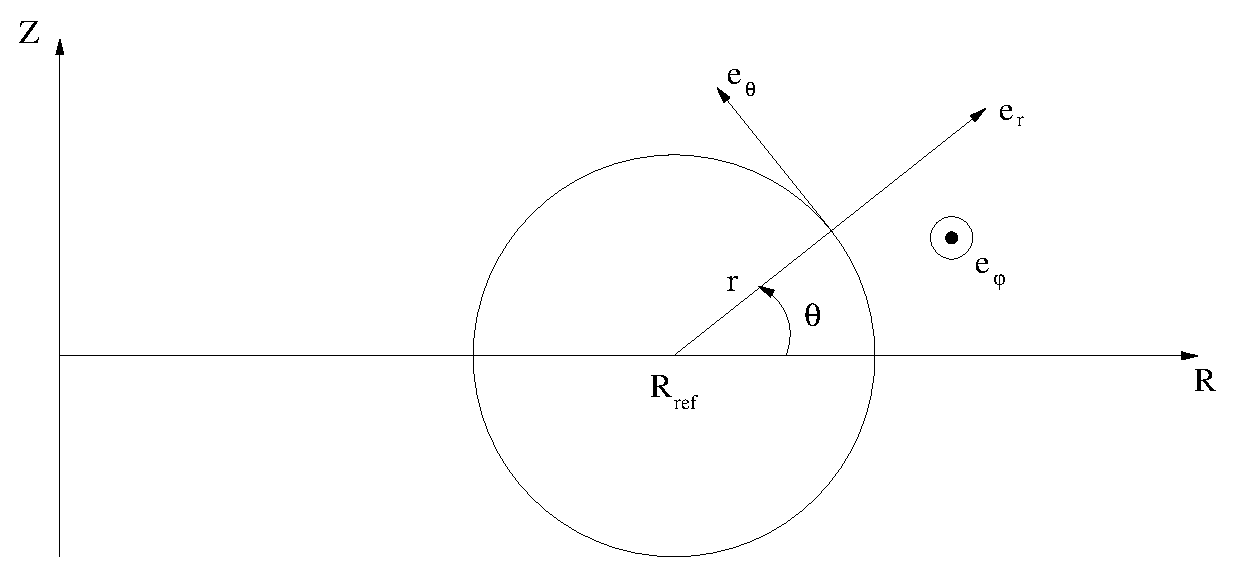
\includegraphics[width=0.6\textwidth]{circFS.eps}
\caption{Circular flux surface centred on $R=R\ind{ref}$, $Z=0$ and $(r,\theta,\varphi)$ coordinates.\label{circFS}}
\end{center}
\end{figure}

In this section, unless explicitly denoted by a $N$ subscript, the various quantities are not normalised. The starting assumption of the model is that the flux surfaces are circular and concentric
with the poloidal flux being a function of the radial coordinate only $\Psi=\Psi(r)$, see
figure~\ref{circFS}. This is a valid assumption in the case of small $\epsilon$ and small $\beta$. It simply means that the terms of order $\epsilon^2$ are neglected and that the Shafranov shift is
considered to be of order $\epsilon^2$.
For simplicity, the various terms are not expanded in $\epsilon$ in the following calculation, but one has to remember that the results are only valid up to order $\epsilon$.
The second assumption of the model is that the radial derivative of the poloidal flux is given by:
\begin{equation}
 \pd{\Psi}{r}=\frac{r B\ind{ref}}{\bar{q}}
\end{equation}
where $B\ind{ref}$ is the value of the magnetic field at $R\ind{ref}$ taken to be the major radius of the magnetic axis (i.e. the centre of the flux surfaces) and $\bar{q}>0$ is a parameter directly
related to the safety factor $q$. The flux surfaces are parametrised by $R=R\ind{ref}+r \cos \theta$ and $Z=r \sin\theta$ in the $(r,\theta,\varphi)$ coordinates system. The inverse aspect ratio is
defined as $\epsilon=r/R\ind{ref}$ and it might be worth reminding that:
\begin{equation}
 \nabla \epsilon = \frac{1}{R\ind{ref}} \mathbf{e_r}, \qquad \nabla \theta = \frac{1}{\epsilon R\ind{ref}}\mathbf{e_\theta}, \qquad \nabla \varphi = \frac{1}{R} \mathbf{e_\varphi}
\end{equation}
Another useful quantity is the Jacobian of the $(\Psi,\theta,\varphi)$ coordinates system which can be expressed as
\begin{equation}
 {J_{\Psi\theta\varphi}}^{-1}=\nabla\Psi\times\nabla\theta\cdot\nabla\varphi=\pd{\Psi}{r}{J_{r\theta\varphi}}^{-1}=\pd{\Psi}{r}\frac{1}{rR}=\frac{B\ind{ref}}{\bar{q}R}
\end{equation}

As usual, the magnetic field is decomposed into its toroidal and poloidal components:
\begin{equation}
 \mathbf{B} = s\ind{B}F(\Psi)\nabla \varphi + s\ind{j} \nabla \varphi \times \nabla \Psi
\end{equation}
One furthermore assumes that $F(\Psi)=R\ind{ref}B\ind{ref}$ and the magnetic field can then be written as
\begin{equation}
 \mathbf{B} = R\ind{ref}B\ind{ref}\left[ s\ind{B} \nabla \varphi + s\ind{j}\frac{1}{\bar{q}}\frac{\epsilon^2}{1+\epsilon\cos\theta}\nabla \theta\right]
\end{equation}
The definition of the safety factor is
\begin{equation}
 q=\frac{1}{2\pi}\int_0^{2\pi}\frac{\mathbf{B}\cdot\nabla\varphi}{\mathbf{B}\cdot\nabla\theta}\,\textrm{d}\theta
\end{equation}
which in the model considered here leads to
\begin{equation}
 q=\frac{1}{2\pi}\int_0^{2\pi}s\ind{B}s\ind{j}J_{\Psi\theta\varphi}\frac{R\ind{ref}B\ind{ref}}{R^2}\,\textrm{d}\theta=s\ind{B}s\ind{j}\frac{\bar{q}}{2\pi}\int_0^{2\pi}
\frac{1}{1+\epsilon\cos\theta}\,\textrm{d}\theta=s\ind{B}s\ind{j}\frac{\bar{q}}{\sqrt{1-\epsilon^2}}
\end{equation}
which makes explicit the relationship between $q$ and $\bar{q}$.

We now have all the ingredients to derive the field aligned coordinates $(\psi,\zeta,s)$. In GKW, $\psi$ is defined to be $\epsilon$ and we will use this notation in the following to avoid possible
confusion with the poloidal flux $\Psi$. The definition of the parallel coordinate $s$ is
\begin{equation}
 s = \int_0^\theta \frac{\textrm{d}\theta}{\mathbf{B}\cdot\nabla\theta} \,\,\Big{/} \int_0^{2\pi} \frac{\textrm{d}\theta}{\mathbf{B}\cdot\nabla\theta}
\end{equation}
So, we first calculate
\begin{equation}
 \int_0^\theta \frac{\textrm{d}\theta}{\mathbf{B}\cdot\nabla\theta} = \int_0^\theta s\ind{j}J_{\Psi\theta\varphi}\,\textrm{d}\theta = s\ind{j}\bar{q}\frac{R\ind{ref}}{B\ind{ref}} \int_0^\theta
[1+\epsilon\cos\theta]\,\textrm{d}\theta = s\ind{j}\bar{q}\frac{R\ind{ref}}{B\ind{ref}} [\theta + \epsilon \sin\theta],
\end{equation}
to get
\begin{equation}
 s=\frac{1}{2\pi}[\theta + \epsilon\sin\theta]
\label{eq:s:def}
\end{equation}
and
\begin{eqnarray}
 \pd{s}{\epsilon} &=& \frac{1}{2\pi}\sin\theta, \\
 \pd{s}{\theta} &=& \frac{1}{2\pi}[1+\epsilon\cos\theta],\\
 \pd{s}{\varphi} &=& 0.
\end{eqnarray}
The definition of the $\zeta$ coordinate is:
\begin{equation}
 \zeta = - \frac{\varphi}{2\pi} + s\ind{B}s\ind{j}\frac{F}{2\pi}\int_0^\theta \frac{J_{\Psi\theta\varphi}}{R^2}\,\textrm{d}\theta 
\end{equation}
which in the ad-hoc circular model gives
\begin{equation}
 \zeta = - \frac{\varphi}{2\pi} + s\ind{B}s\ind{j}\frac{\bar{q}}{2\pi}\int_0^\theta \frac{\textrm{d}\theta}{1+\epsilon\cos\theta}
\end{equation}
Noticing that
\begin{equation}
 \int_0^\theta \frac{\textrm{d}\theta}{1+\epsilon\cos\theta} = \frac{2}{\sqrt{1-\epsilon^2}}\arctan\left[ \sqrt{\frac{1-\epsilon}{1+\epsilon}}\tan \frac{\theta}{2}\right],
\end{equation}
one gets
\begin{equation}
 \zeta = - \frac{\varphi}{2\pi} + s\ind{B}s\ind{j}\frac{|q|}{\pi}\arctan\left[ \sqrt{\frac{1-\epsilon}{1+\epsilon}}\tan \frac{\theta}{2}\right]
 \label{eq:def:zeta}
\end{equation}
and
\begin{eqnarray}
 \pd{\zeta}{\epsilon} &=& s\ind{B}s\ind{j}\frac{|q|}{\epsilon\pi}\left[ \hat{s}\arctan\left[ \sqrt{\frac{1-\epsilon}{1+\epsilon}}\tan \frac{\theta}{2}\right] -
\frac{\epsilon\tan\frac{\theta}{2}}{\sqrt{1-\epsilon^2}\left(1+\epsilon+(1-\epsilon)\tan^2\frac{\theta}{2}\right)} \right], \\
 \pd{\zeta}{\theta} &=& s\ind{B}s\ind{j}\frac{|q|}{2\pi}\frac{\sqrt{1-\epsilon^2}}{1+\epsilon\cos\theta},\\
 \pd{\zeta}{\varphi} &=& -\frac{1}{2\pi}.
\end{eqnarray}
From the decomposition of $\nabla s$ and $\nabla \zeta$ as a function of $\nabla \epsilon$, $\nabla \theta$ and $\nabla\varphi$
\begin{eqnarray}
 \nabla s &=& \pd{s}{\epsilon} \nabla\epsilon +  \pd{s}{\theta} \nabla\theta +  \pd{s}{\varphi} \nabla\varphi \\
 \nabla \zeta &=& \pd{\zeta}{\epsilon} \nabla\epsilon +  \pd{\zeta}{\theta} \nabla\theta +  \pd{\zeta}{\varphi} \nabla\varphi ,
\end{eqnarray}
the calculation of the metric tensor is straightforward:
\begin{eqnarray}
 g^{\epsilon\epsilon}_N &= R\ind{ref}^2 g^{\epsilon\epsilon} &= 1,\\
 g^{\epsilon\zeta}_N &= R\ind{ref}^2 g^{\epsilon\zeta} &= \pd{\zeta}{\epsilon},\\
 g^{\epsilon s}_N &=R\ind{ref}^2 g^{\epsilon s} &= \frac{1}{2\pi}\sin\theta,\\
 g^{\zeta\zeta}_N &= R\ind{ref}^2 g^{\zeta\zeta} &= \left[\pd{\zeta}{\epsilon}\right]^2 + \left[\frac{1}{2\pi}\frac{1}{1+\epsilon\cos\theta} \right]^2
\left[1+\frac{q^2}{\epsilon^2}(1-\epsilon^2)\right]\\
 g^{\zeta s}_N &= R\ind{ref}^2 g^{\zeta s} &= \frac{\sin\theta}{2\pi}\pd{\zeta}{\epsilon} + s\ind{B}s\ind{j}\frac{|q|}{(2\pi\epsilon)^2}\sqrt{1-\epsilon^2}\\
 g^{s s}_N &= R\ind{ref}^2 g^{s s} &= \frac{1}{4\pi^2}\left[ 1 + \frac{2}{\epsilon}\cos\theta + \frac{1}{\epsilon^2}\right].
\end{eqnarray}
To calculate the other metric elements one needs the norm of the magnetic field
\begin{equation}
 B=\sqrt{\mathbf{B}\cdot\mathbf{B}}=\frac{B\ind{ref}}{1+\epsilon\cos\theta}\left[ 1+ \frac{1}{q^2}\frac{\epsilon^2}{1-\epsilon^2} \right]^{1/2}
\end{equation}
and its gradient
\begin{equation}
 \nabla B = \pd{B}{\epsilon} \nabla \epsilon + \pd{B}{\theta} \nabla \theta
\end{equation}
which involves
\begin{eqnarray}
 \pd{B}{\epsilon} &=&  \left[ -\frac{\cos\theta}{1+\epsilon\cos\theta} + \frac{\epsilon}{\epsilon^2+q^2(1-\epsilon^2)}(1-\hat{s}+\frac{\epsilon^2}{1-\epsilon^2})\right]B\\
 \pd{B}{\theta} &=& \frac{\epsilon\sin\theta}{1+\epsilon\cos\theta}B
\end{eqnarray}
From the definition 
\begin{equation}
 \mathcal{D}^\alpha_N = \frac{R\ind{ref}^2}{B^2B_N}\mathbf{B}\times\nabla B \cdot \nabla x^\alpha
\end{equation}
and some straightforward algebra (which has to be understood as ``I am by far too lazy to write down all the steps in \LaTeX'') we get the components of the tensor related to the curvature and
$\nabla B$ drift:
\begin{eqnarray}
 \mathcal{D}^{\epsilon}_N &=& -s\ind{B} \sin\theta \frac{1}{1+\frac{1}{q^2}\frac{\epsilon^2}{1-\epsilon^2}} \\
 \mathcal{D}^{\zeta}_N &=& \left[\frac{s\ind{j}}{2\pi} \frac{1}{B}\pd{B}{
\epsilon}\left(\frac{|q|\sqrt{1-\epsilon^2}}{\epsilon}+\frac{\epsilon}{|q|\sqrt{1-\epsilon^2}}\right)-s\ind{B}\pd{\zeta}{\epsilon}\sin\theta \right]
\frac{1}{1+\frac{1}{q^2}\frac{\epsilon^2}{1-\epsilon^2}}\\
 \mathcal{D}^{s}_N &=& \frac{s\ind{B}}{2\pi}\left[\frac{1}{\epsilon B}\pd{B}{\epsilon}(1+\epsilon\cos\theta)^2 -\sin^2\theta\right]
\frac{1}{1+\frac{1}{q^2}\frac{\epsilon^2}{1-\epsilon^2}}\\
\end{eqnarray}
The tensor related to the $\mathbf{E}\times\mathbf{B}$ drift can be obtained from the metric tensor elements:
\begin{equation}
 \mathcal{E}^{\alpha\beta}_N = s\ind{j}\frac{\pi R\ind{ref}^2}{BB_N}\pd{\Psi}{\epsilon}(g^{\alpha\epsilon} g^{\beta\zeta} - g^{\alpha\zeta} g^{\beta\epsilon})
\end{equation}
which for the ad-hoc model gives:
\begin{equation}
 \mathcal{E}^{\alpha\beta}_N = s\ind{j}\frac{\pi }{B_N^2}\frac{\epsilon}{|q|\sqrt{1-\epsilon^2}}(g^{\alpha\epsilon}_N g^{\beta\zeta}_N - g^{\alpha\zeta}_N g^{\beta\epsilon}_N)
\end{equation}
We the calculate the tensor related to the parallel derivative 
\begin{equation}
 \mathcal{F}_N = R\ind{ref} \frac{\mathbf{B}\cdot\nabla s}{B} = \frac{s\ind{j}}{2\pi |q| B_N}\frac{1}{\sqrt{1-\epsilon^2}}
\end{equation}
and the tensor related to the trapping
\begin{equation}
 \mathcal{G}_N = \frac{R\ind{ref}\mathbf{B}\cdot\nabla B}{B^2} = s\ind{j}\frac{\epsilon B_N \sin \theta}{|q|\sqrt{1-\epsilon^2}}\frac{1}{1+\frac{1}{q^2}\frac{\epsilon^2}{1-\epsilon^2}}.
\end{equation}
For the tensor related to the Coriolis drift
\begin{equation}
 \mathcal{H}^\alpha_N=\frac{R\ind{ref}}{B_N\Omega}\mathbf{\Omega}_\perp\cdot\nabla x^\alpha,
\end{equation}
we first decompose $\mathbf{\Omega}$ as
\begin{equation}
 \mathbf{\Omega} = -s\ind{B}\Omega\nabla Z = -s\ind{B}R\ind{ref}\Omega\left[ \sin\theta \nabla \epsilon + \epsilon \cos \theta \nabla \theta\right]
\end{equation}
to get
\begin{equation}
 \mathbf{\Omega}\cdot\mathbf{b} = -s\ind{B}s\ind{j}\Omega\frac{\epsilon\cos\theta}{|q|\sqrt{1-\epsilon^2}}\frac{R\ind{ref}B\ind{ref}}{RB} 
\end{equation}
and finally obtain
\begin{eqnarray}
 \mathcal{H}^\epsilon_N &=& -\frac{s\ind{B}}{B_N}\sin\theta \\
 \mathcal{H}^\zeta_N &=& -\frac{s\ind{B}}{B_N}\sin\theta\pd{\zeta}{\epsilon} -
                         \frac{s\ind{j}|q|\cos\theta}{2\pi\epsilon B_N}\frac{\sqrt{1-\epsilon^2}}{1+\epsilon\cos\theta}\\
 \mathcal{H}^s_N &=& -\frac{s\ind{B}}{2\pi B_N}\sin^2\theta + \frac{s\ind{B}}{2\pi B_N}(1+\epsilon\cos\theta)\left[ -\frac{\cos\theta}{\epsilon} + \frac{\epsilon\cos\theta}{q^2(1-\epsilon^2)}
\frac{1}{1+\frac{1}{q^2}\frac{\epsilon^2}{1-\epsilon^2}}\right].
\end{eqnarray}
Using
\begin{equation}
 \nabla R = R\ind{ref} \left[\cos\theta \nabla \epsilon -\epsilon\sin\theta\nabla\theta \right] 
\end{equation}
the tensor related to the centrifugal drift, can be expressed as
\begin{equation}
 \mathcal{I}^\alpha_N = s\ind{j}\frac{2\pi}{B_N^2}\frac{\epsilon(1+\epsilon\cos\theta)}{|q|\sqrt{1-\epsilon^2}}\left[g^{\epsilon\alpha}_N\left[\cos\theta\pd{\zeta}{\epsilon} -
s\ind{B}s\ind{j}\frac{|q|}{2\pi\epsilon}\frac{\sin\theta\sqrt{1-\epsilon^2}}{1+\epsilon\cos\theta}\right] -g^{\zeta\alpha}_N\cos\theta\right]
\end{equation}
We also have
\begin{equation}
 {\cal M} = {1 \over q \sqrt{1-\epsilon^2}}\left(1-{\epsilon \over 1-\epsilon^2}-{\hat s \over q}\right).
\end{equation}
Finally, the elements used to calculate the centrifugal potential are 
\begin{equation}
 \mathcal{J}_N= (1+\epsilon\cos\theta)^2-\frac{R_0^2}{R\ind{ref}^2} \qquad \mathcal{K}_N=\pd{\mathcal{J}_N}{
\epsilon} \biggr |_s =2(\cos\theta+\epsilon)-{\cal L}_N
\end{equation}
where the transformation between partial deriviatives at constant $\theta$ and $s$ gives
\begin{equation}
\frac{1}{R\ind{ref}} \pd{R}{\epsilon} \biggr |_s= \cos(\theta) + \frac{\epsilon \sin^2(\theta)}{1+\epsilon \cos(\theta)}
\end{equation}
which has been used to calculate ${\cal K}$.
The two choices for $R_0$ (magnetic axis value or $R(s=0)$) give
\begin{equation}
R_0=R\ind{ref} \Rightarrow {\cal L}_N=0, \quad  
R_0=(1+\epsilon)R\ind{ref} \Rightarrow {\cal L}_N =2(1+\epsilon)
\end{equation}
respectively.

% \subsection{Shifted circular surface geometry} 
% (NOT IMPLEMENTED, NOT CONSISTENT WITH OTHER SECTIONS - not normalised, definitions of Rref and r0 differ)\\
% 
% The shifted circular surface geometry is defined in the ($R,Z$) plane (using cylindrical coordinates
% $(R,\phi,z)$. 
% \begin{equation} 
% R = r \cos \theta + \Delta(r) + R_0 \qquad {\rm with} \qquad \Delta(0) = 0 
% \end{equation}
% \begin{equation} 
% Z = r \sin \theta
% \end{equation}
% Surfaces of constant $r$ are assumed to be flux surfaces. One can confusingly define two major 
% radii. One is the radius of the magnetic axis $R_0$, and one is the major radius of the centre 
% of the surface $R_c$ 
% \begin{equation} 
% R_c = (R(\theta =0) + R(\theta = \pi) )/2 = R_0 + \Delta(r) 
% \end{equation}
% Since the first one is a constant while $R_c$ depends on $r$, we will choose to normalise all 
% the radii with $R_0$, i.e. 
% \begin{equation} 
% R_{\rm ref} = R_0
% \end{equation}
% The normalised radial coordinate then is 
% \begin{equation} 
% \psi = r / R_0 = \epsilon
% \end{equation}
% and we will define a normalised major radius that gives the centre of the surface as 
% \begin{equation} 
% R_{cN} = 1 + {\Delta (r) \over R_0} 
% \end{equation}
% 
% From the equations above one can work out
% \begin{equation} 
%   \bbmatrix
%     \nabla r      \\
%     \nabla \theta
%   \ebmatrix
%   = {1\over r (1 + \Delta^\prime \cos \theta)} 
%   \bbmatrix
%     r \cos \theta & r \sin \theta \\
%     - \sin \theta & \Delta^\prime + \cos \theta
%    \ebmatrix
%    \bbmatrix
%      \nabla R \\
% 	 \nabla Z
%    \ebmatrix 
% \end{equation}
% where 
% \begin{equation}
%   \Delta^\prime = {{\rm d} \Delta \over {\rm d} r} 
% \end{equation}
% The poloidal magnetic field can be written as 
% \begin{equation} 
% {\bf B}_p = B_p {{\bf e}_\theta \over \vert {\bf e}_\theta \vert} \qquad 
% {\bf e}_\theta = \pd{{\bf x}}{\theta} =
% \bbmatrix
%   -r \sin \theta \\
%    r \cos \theta
% \ebmatrix  
% \end{equation} 
% From which it folows that 
% \begin{equation} 
% {\bf e}_\theta \cdot \nabla \theta = 1 \qquad {\bf B} \cdot \nabla \theta = B_p / r 
% \end{equation} 
% From flux conservation 
% \begin{equation} 
% R B_p {\rm d}l_\perp = {R B_p \over \vert \nabla r \vert } {\rm d} r = {\rm constant} 
% \end{equation}
% It follows that  
% \begin{equation} 
% {B_p \over B_p(\pi/2)} = {R_{cN}(\psi) \over (1 + \Delta^\prime(\psi) \cos \theta) (R_{cN}(\psi) + \psi \cos \theta)}
% \end{equation}
% The integral to obtain $s$ and $B^s$ can be easily performed 
% \begin{equation} 
% B^s = {B_p(\pi/2)\over 2 \pi ( 1 + \psi \Delta^\prime / 2 R_{Nc} )}
% \end{equation}
% \begin{equation} 
% s = {\theta \over 2 \pi} + {2 \psi \sin \theta + 2 \Delta^\prime R_{cn} \sin \theta + \Delta^\prime \psi 
% \cos \theta \sin \theta \over 4 \pi R_{cn} ( 1 + \Delta^\prime \psi / 2 R_{cn})}
% \end{equation}
% After some manipulations also the flux surface average of $1/R^2$ can be expressed as 
% \begin{equation} 
% \biggl \langle {1 \over R^2} \biggr \rangle = {1\over R_0^2} {1 \over R_{cN} + \psi \Delta^\prime / 2} 
% \biggl [ {1 - \Delta^\prime \over \sqrt{R_{cN}^2 - \psi^2} } + {\Delta^\prime \over \psi} \biggr ] 
% \end{equation}

\subsection{Miller parametrisation}
Miller parametrisation of the flux surface shape is a good compromise between the flexibility of the circ geometry and the precision of an equilibrium obtained from the solutin of the Grad-Shafranov equation.
In this section the Miller parametrisation first done in \cite{MIL98} is described. Then the derivation of the metric tensor in GKW coordinate system ($\psi,\zeta,s$) and the derivatives of the magnetic field are shown using the implementation method of \cite{CAN09}. \\
To avoid any confusion between the poloidal magnetic flux and the radial coordinate the latter will be called $r$ through the entire section.  For the miller geometry, $R_{\rm ref} = (R_{\rm max} + R_{\rm min})/2 $ which is the geometric axis of the flux surface in question.

\subsubsection{Parametrisation (Input List)}
The following parameters are used to describe a magnetic flux surface in (R,Z) plane : $\kappa$ (elongation), $\delta$ (triangularity), $\zeta$ (squareness), $R_{\rm mil}$, $Z_{\rm mil}$, and their radial derivatives $s_\kappa, s_\delta ($definition of$ \cite{MIL98}), s_\zeta, {\mathrm{d} R_{
\rm mil} \over \mathrm{d}r}$, ${\mathrm{d}Z_{\rm mil} \over \mathrm{d}r}$ defined such that:  
\begin{equation}
s_\kappa  =  {r \over \kappa}{\mathrm{d}\kappa \over \mathrm{d}r}, \qquad
s_\delta  =  r{{\mathrm{d}\delta \over \mathrm{d}r} \over \sqrt{1-\delta^2}}, \qquad
s_\zeta  = r{\mathrm{d}\zeta \over \mathrm{d}r}
\end{equation}
Parameters such as ${\mathrm{d} p \over \mathrm{d} \Psi}$ (pressure gradient), q (safety factor), $\hat s$ (magnetic shear) and $\epsilon$ (aspect ratio $= {r \over R_{
\rm mil}}$) are also used.
Flux surfaces geometry are then given by :
\begin{eqnarray}
R &=& R_{\rm mil} + r \cos{(\theta + \arcsin \delta \sin \theta)} \\
Z &=& Z_{\rm mil} + r \kappa \sin{(\theta + \zeta \sin{2\theta})}
\end{eqnarray}
and the radial derivatives of R and Z by :
\begin{eqnarray}
\pd{ R}{r} &=& {\mathrm{d}R_{\rm mil} \over \mathrm{d}r} + \cos{(\theta + \arcsin \delta \sin \theta)} - s_\delta \sin{\theta} \sin{(\theta + \arcsin \delta \sin \theta)} \\
\pd{ Z}{r} &=& {\mathrm{d}Z_{\rm mil} \over \mathrm{d}r} + \kappa \sin{(\theta + \zeta \sin{2\theta})} + \kappa s_\kappa \sin{(\theta + \zeta \sin{2\theta})} + \kappa s_\zeta \sin{(2\theta)} \cos{(\theta + \zeta \sin{2\theta})}
\end{eqnarray}
Examples how the parameters affect the cross section of a flux surface can be
seen in Fig.~\ref{fig:examplemillergeom}.
\begin{figure}
  \begin{center}
    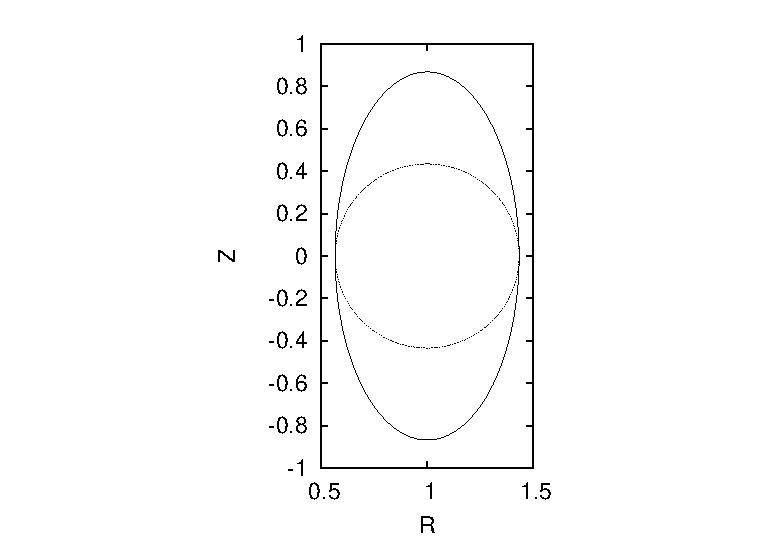
\includegraphics[width=0.49\textwidth]{millergeomkappa}
    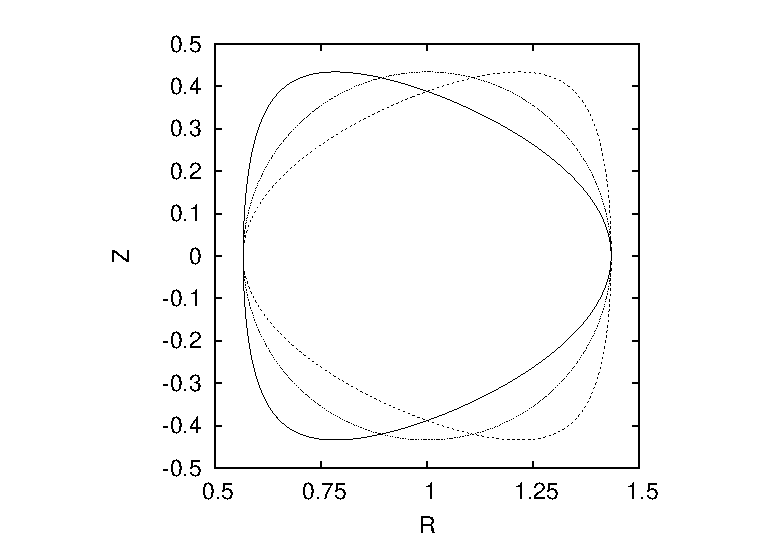
\includegraphics[width=0.49\textwidth]{millergeomdelta}
    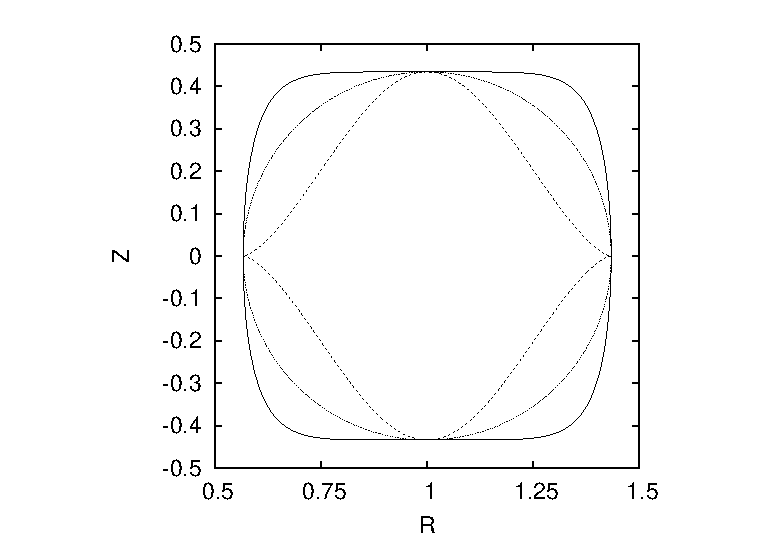
\includegraphics[width=0.49\textwidth]{millergeomzeta}
    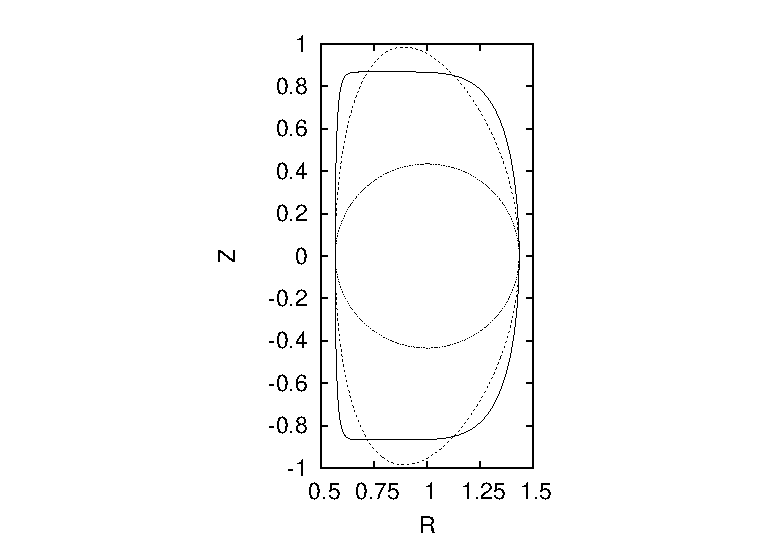
\includegraphics[width=0.49\textwidth]{millergeomall}
    \caption[Examples Miller geometry]{\label{fig:examplemillergeom}
    Examples for the effects of $\kappa$, $\delta$ and $\zeta$ in Miller
    geometry. In all plots shown in this drawing, the dashed line is a circular flux surface.
    Top left: $\kappa=2.0$, $\delta=\zeta=0.0$. Top right: The
    full/dashed line has $\delta=\pm 0.5$, $\kappa=1.0$ and $\zeta=0.0$. Bottom
    left: The full/dashed line has $\zeta=\pm 0.5$, $\kappa=1$ $\delta=0.0$.
    Bottom right: The full line has $\kappa=2$, $\delta=0.5$ and $\zeta=0.5$.
    The dashed line is an example taken from an actual experiment
    with $\kappa=2.25$, $\delta=0.25$, $\zeta=-0.016$.}
  \end{center}
\end{figure}
The pressure gradient can be computed from different parameters through the input \textit{gradp\_type}.
The input list is also defined in the file \doc{input.dat.sample}.

The normalisation is made such that:
\begin{eqnarray}
R_N &=& 1 + \epsilon \cos (\theta + \arcsin \delta \sin \theta) \\
F_N &=& 1
\end{eqnarray}
We have then $R_{\rm ref} = R_{\rm mil}$ and $B_{\rm ref} = B_t(R_{\rm mil})$. \\
The normalisation for the plasma pressure gradient is given here using :
\begin{equation}
\left({\mathrm{d} p \over \mathrm{d} \Psi}\right)_N = {2 \mu_0 R_{\rm ref}^2\over B_{\rm ref}} {\mathrm{d} p \over \mathrm{d} \Psi}
\end{equation}
The normalised pressure gradient used in the code can be given by :
\begin{eqnarray}
\left({\mathrm{d} p \over \mathrm{d} \Psi}\right)_N &=& - \alpha {\left(2\pi^2\right) \over \left(\partial_{\Psi}V\right)_N } \left({V_N \over 2\pi ^2}\right)^{-1/2}\\
\left({\mathrm{d} p \over \mathrm{d} \Psi}\right)_N &=& {\alpha_{MHD}\over \epsilon ^2}\left({\mathrm{d} \Psi \over \mathrm{d} \epsilon}\right)_N \\
\left({\mathrm{d} p \over \mathrm{d} \Psi}\right)_N &=& {\beta ' \over 2 {\mathrm{d} \Psi_N \over \mathrm{d} \epsilon}}
\end{eqnarray}
with $\alpha$ taken from equation 42 in \cite{MIL98}, $\alpha_{MHD}$ from equation 141 \cite{CAN09} and $\beta '$ is defined in section \ref{Sec:betabetapr}. \\
For centrifugal effects on the pressure gradient go to equation \ref{eq:rota}. \\
The equations used below are not normalised however they are in the code. \\
In the coordinate system $(r,\theta,\varphi)$ where the magnetic flux surfaces are described, the elements of the metric tensor are :
\begin{eqnarray}
g_{rr} &=& \left(\pd{ R}{r}\right)^2 + \left(\pd{ Z}{r}\right)^2, \\
g_{r \theta} &=& \pd{ R}{r}\pd{ R}{\theta} + \pd{ Z}{r}\pd{ Z}{\theta} \\
g_{\theta \theta} &=& \left(\pd{ R}{\theta}\right)^2 + \left(\pd{ Z}{\theta}\right)^2, \\
g_{\varphi \varphi} &=& R^2
\end{eqnarray}
The contravariant metric tensor, used to calculate the contravariant metric tensor of the GKW basis, is deduced from the relation $g_{ij} \cdot g^{ij} = I$ with I the identity matrix.
\subsubsection{Mercier-Luc coordinate system}
An expansion of the poloidal flux $\Psi$ is needed. A coordinate system (introduced by Mercier-Luc) is defined such that the expansion is easy to use (orthogonal system ($\rho,l,\varphi$)).
\begin{figure}[h]
\begin{center}
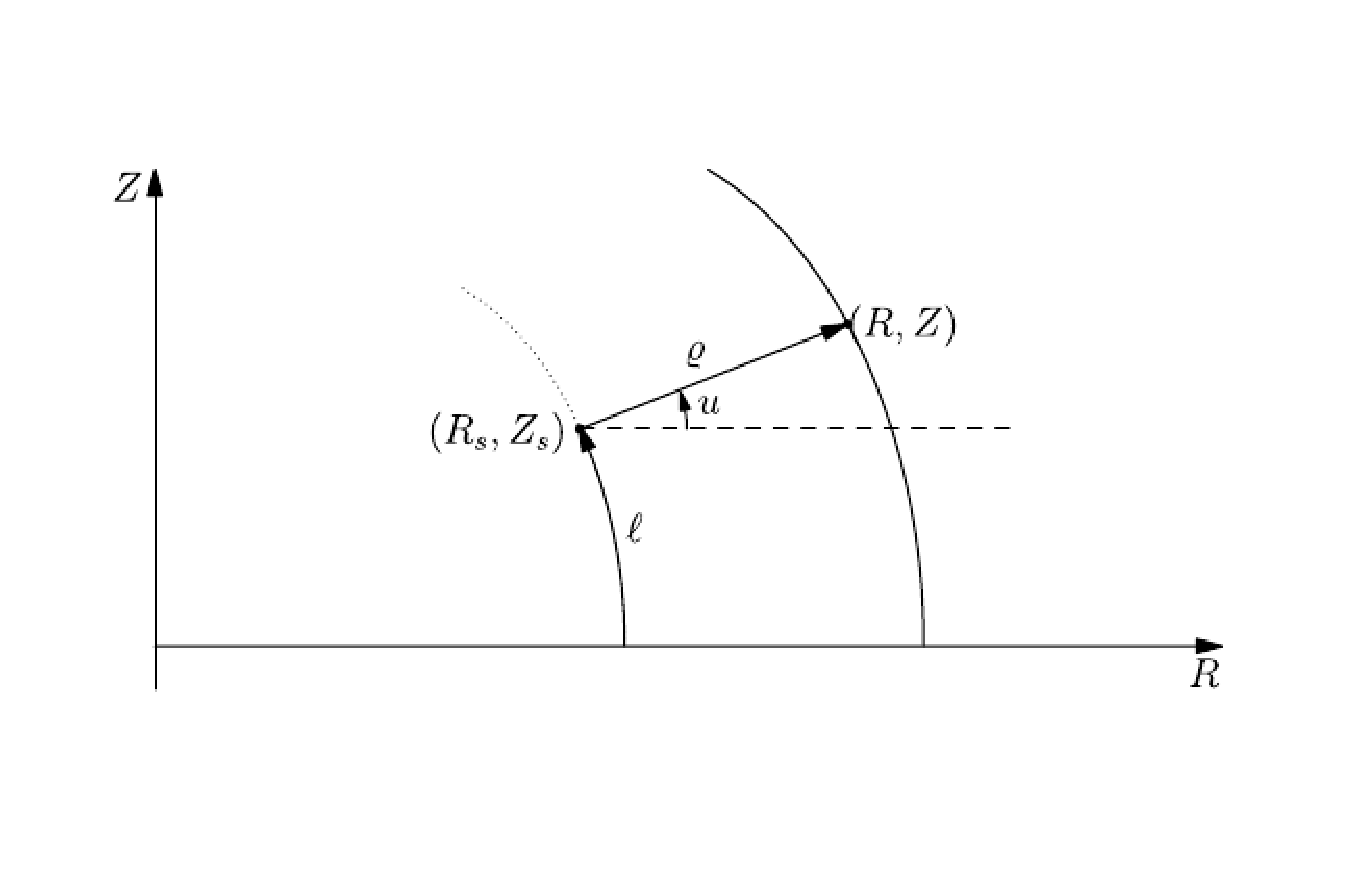
\includegraphics[width=0.6\textwidth]{mercier-luc.eps}
\caption{Mercier-Luc coordinate system.\label{merc-luc}...from \cite{CAN09}}
\end{center}
\end{figure}
In addition to the plasma shape, 
the gradient of the plasma pressure must also be specified, which in GKW can be done independently for the geometry, or by coupling to $\beta^\prime$.

\begin{eqnarray}
\Psi &=& \Psi_s + \rho \Psi_1 + \rho^2 \Psi_2 \\
R &=& R_s + \rho \cos{u} \\
Z &=& Z_s + \rho \sin{u}
\end{eqnarray}
with 
\begin{eqnarray}
\cos u &=& \pd{ Z_s}{l} \\
\sin u &=& - \pd{ R_s}{l}
\end{eqnarray}
where the subscript s means the value on the surface of consideration. \\
The metric elements are: 
\begin{eqnarray}
g_{\rho \rho} &=& 1 \\
g_{ll} &=& \left(1 + {\rho \over r_c} \right) \\
g_{\varphi \varphi} &=& R^2
\end{eqnarray}
The Jacobian is then:
\begin{equation}
J_\rho = R \left(1 + {\rho \over r_c}\right) 
\end{equation}
with $r_c$ being the curvature radius :
\begin{equation}
r_c = g_{\theta \theta}^{3/2} \left(\pd{ R}{\theta}\pdd{Z}{ \theta}-\pd{ Z}{\theta}\pdd{R}{\theta}\right)^{-1} 
\end{equation}
To switch from $(\rho,l,\varphi)$ to $(r,\theta,\varphi)$ the following relations are important (all quantities are taken on the flux surface)  :
\begin{eqnarray}
\pd{ \rho}{r} &=& \cos u \pd{ R}{r} + \sin u \pd{ Z}{r} \\
\pd{ l}{r} &=& \cos u \pd{ Z}{r} - \sin u \pd{ R}{r} \\
\pd{ \rho}{\theta} &=& 0 \\
\pd{ l}{\theta} &=& \sqrt{g_{\theta \theta}}
\end{eqnarray}
From the definition of the poloidal magnetic field:
\begin{equation}
B_p^2 = |\nabla \varphi|^2|\nabla \Psi|^2 = {\Psi_1 ^2 \over R_s ^2 }
\end{equation}
one finds
\begin{equation}
\Psi_1 = R_s B_{ps}
\end{equation}
$\Psi_2$ is obtained from the Grad-Shafranov equation for the expansion of $\Psi$:
\begin{equation}
R \nabla \cdot{\nabla \Psi \over R^2} = -\mu_0 R^2 p'(\Psi) - FF'(\Psi)
\end{equation}
with ' corresponding to the derivative toward the poloidal magnetic flux.
One can easily obtain: 
\begin{equation}
\Psi_2 = {1 \over 2}\left(B_p \cos u - {B_p R \over r_c} - \mu_0 R^2 p' - FF'\right)
\end{equation}
From this point we see that we have other parameters : $F$ (see the normalisation section), $F'$, $p'$, ${d \Psi \over dr}$ that we need to link to our first set of parameters.
The relation for $F'$ will be expressed later (it is not trivial).
\subsubsection{Relations for $p'$ and ${d\Psi \over dr}$}
${d\Psi \over dr}$ is obtained from the definition of $q$:
\begin{equation}
q = {1 \over 2 \pi} \int_0^{2\pi} {{{\bf B} \cdot \nabla \varphi \over {\bf B} \cdot \nabla \theta}\mathrm{d}\theta} 
\end{equation}
with 
\begin{equation}
{\bf B} = s_B F \nabla \varphi + s_J \nabla \varphi \times \nabla \Psi
\end{equation}
It follows : 
\begin{equation}
q = s_B s_J{F \over 2 \pi {\mathrm{d}\Psi \over \mathrm{d}r}} \int_0^{2\pi}{{J_r \over R^2}\mathrm{d}\theta}
\end{equation}
yields 
\begin{equation}
{\mathrm{d}\Psi \over \mathrm{d}r} = s_B s_J{F \over 2 \pi q} \int_0^{2\pi}{{J_r \over R^2}\mathrm{d}\theta}
\end{equation}
Numerical integrals are implemented using Simpson's method. \\
$p'$ is given from the relation in \cite{MIL98}:
\begin{equation}
\alpha = -{2\pd{ V}{\Psi} \over (2 \pi)^2}\left({V \over 2 \pi^2 R_{
\rm mil}}\right)^{1/2} \mu_0 p^\prime
\end{equation}
V is the volume defined by the magnetic flux surface :
\begin{equation}
V = 2 \pi S R_G
\end{equation}
with
\begin{eqnarray}
R_G &=& {\int_0^{2\pi} {R \sqrt{(\pd{ R}{\theta})^2 + (\pd{ Z}{\theta})^2} \mathrm{d}\theta} \over \int_0^{2\pi} {\sqrt{(\pd{ R}{\theta})^2 + (\pd{ Z}{\theta})^2} \mathrm{d}\theta}} \\
S &=& \int_0^{2\pi} {Z\pd{ R}{\theta}}
\end{eqnarray}
$\pd{ V}{\Psi}$ can easily be defined analytically by differentiating towards $r$ and using ${\mathrm{d}\Psi \over \mathrm{d}r}$ \\
\\
 
\subsubsection{Effect of toroidal rotation on the magnetic equilibrium}
Force balance equation for species a:

\begin{align}
m_an_a\left(\pd{}{t}+V_a\cdot \nabla \right)V_a = -\nabla p_a - \nabla \cdot \pi_a + e_a n_a\left(E+V_a\times B\right)+R_a
\end{align}

Viscosity $\nabla \cdot \pi_a$ and friction $R_a$ are being neglected. \\
A two species model with singly (for now) charged ions is considered (trace species can be added but won't affect the magnetic equilibrium: $m_tn_t \ll m_in_i$, i being the main ion species). Using $m_e \ll m_i$ and taking the dot product of force balance equation with $\mathbf b$, one obtains:

\begin{align}
n_e &= n_{R_0,e}\exp{\left({e \Phi \over T_e}\right)} \\
n_i &= n_{R_0,i}\exp{\left({-e \Phi \over T_i }+ {m_i\Omega^2(R^2 - R_0^2)\over 2T_i}\right)}
\end{align}

$T_i$ is supposed to be a flux function (might not be always the case \cite{THYA06}) \\
Using Quasineutrality and $T_e \sim T_i$:
\begin{align}
e\phi = {T_e \over T_e + T_i}{m_i \over T_i}{1 \over 2}\Omega^2\left(R^2-R_0^2\right)
\end{align}

The total pressure is then:
\begin{align}
p = Tn\exp{\left({m_i\Omega^2 \over 2 T}(R^2-R_0^2)\right)}
\end{align}

with $T = T_e + T_i$.\\
Furthermore the Grad-Shafranov is modified ($\Psi$ and $R^2$ are regarded as independant variables \cite{THYA06}):
\begin{equation}
R^2 \nabla \cdot \left({\nabla \Psi \over R^2}\right) = -\mu_0 R^2 \pd{ p \left(\Psi,R^2\right)}{\Psi} - FF'
\end{equation}

In normalised units one gets 
\begin{align} \label{eq:rota}
\left(\pd{ p}{\Psi}\right)_N &= {1 \over 2}\left[\beta' + \beta_{ref} n_Rm_{R,i}
\left(\left(R_N^2-R_0^2\right)\left(-2u_N' \Omega + {T_{R,e}{R\over L_{T_e}} + T_{R,i}{R \over L_{T_i}}\over \left(T_{R,e}+T_{R,i}\right)}\right)\right.\right. \nonumber \\
&\left.\left.\left. -R_0\pd{ R_0}{\epsilon}\Omega^2\right)\right)\right]\left({d \psi \over d \Psi}\right)_N\exp{\left({m_{R,i}\Omega_N^2 \over \left(T_{R,e}+T_{R,i}\right)}\left(R_N^2-R_0^2\right)\right)}
\end{align}

From this definition, it enters normalised Grad-Shafranov equation through:
\begin{equation}
\left(R^2 \nabla \cdot \left({\nabla \Psi \over R^2}\right)\right)_N = - R_N^2 \left(\pd{ p \left(\Psi,R^2\right)}{\Psi}\right)_N - F_NF_N'
\end{equation}


$\beta'$ is given in SPCGENERAL. $\beta_{ref}$ can be taken from SPCGENERAL but can also be given using the GEOM parameter \textit{beta\_rota\_miller\_type = 'geom'} and specifying the value in \textit{beta\_rota\_miller}. The other parameters are taken from SPECIES and ROTATION namelists.


\textbf{Modification of the curvature drift}

The magnetic curvature can be recast as:
\begin{eqnarray}
\kappa &=& - \mathbf b \times \left(\nabla \times {\mathbf B \over B} \right) \\
\kappa &=& - {1 \over B} \mathbf{b}\times \left(\nabla \times \mathbf{B}\right) - \mathbf{b} \times \left[\nabla\left({1 \over B}\right) \times \mathbf{B}\right] \\
\kappa &=& {\mu_0 J\times B \over B^2}+{\nabla_\bot \mathbf B \over B} \\
\end{eqnarray}

We will now only consider:
\begin{align}
\kappa_1 = \mu_0 {J \times B \over B^2}
\end{align}
since the term $\nabla_\bot B$ is not modified by rotation.\\

Without rotation 
\begin{align}
J\times B = \nabla p
\end{align}
which leads to the $\beta'$ correction.

For strong toroidal rotation one obtains for a two fluid model with singly charged ions:

\begin{align}
J\times B = -m_in_iR\Omega^2\nabla R + \pd{ p}{\Psi} {d \Psi \over d \psi}\nabla \psi + \pd{ p}{R^2} \nabla R^2
\end{align}

The curvature enters Vlasov equation through
\begin{align}
\left(\kappa_1 \times \nabla f\right)\cdot \mathbf{b} = {\mu_0 \over B^2}\left[\left(m_in_i\Omega ^2-2\pd{ p}{R^2}\right) \left(Bs_B\pd{ f}{x_\alpha}\mathcal{I}^\alpha\right)+2\pd{ p}{\Psi}{d \Psi \over d \psi} \pd{ f}{x_\beta} \mathcal{E}^{\psi \beta}\right]
\end{align}

\subsubsection{Determination of $\nabla s$}
We start from the expression of the magnetic field to express the contravariant component $B^s$ in the coordinate system $(\Psi,l,\varphi)$.
\begin{eqnarray}
B^s(\Psi) &=& B \cdot \nabla s \\
&=& B \cdot \nabla l \pd{ s}{l} \\
\pd{ s}{l} &=& B^s {1 \over B \cdot \nabla l}
\end{eqnarray}
Furthermore : 
\begin{equation}
\int_0^L {\pd{ s}{l'}\mathrm{d}l'} = 1 = B^s \int_0^L {{1 \over B \cdot \nabla l'}\mathrm{d}l'}
\end{equation}
with L being the arclength corresponding to $\theta = 2 \pi$.
Hence
\begin{equation}
B^s = {1 \over \int_0^L {{1 \over B \cdot \nabla l'}\mathrm{d}l'}}
\end{equation}
One gets the expression of $s$ in this basis:
\begin{equation}
s = B^s \int_0^l {{1 \over B \cdot \nabla l'}\mathrm{d}l'}
\end{equation}
Using the expansion of the magnetic flux:
\begin{eqnarray}
B \cdot \nabla l &=& s_B F\nabla \varphi \cdot \nabla l + s_j \nabla \varphi \times \left[(\Psi_1 + 2 \rho \Psi_2)\nabla \rho + \rho \pd{ \Psi_1}{l} \nabla l\right] \cdot \nabla l \\
B \cdot \nabla l &=& s_j {\Psi_1 + 2 \rho \Psi_2 \over J_\rho} \\
B \cdot \nabla l &=& s_j {\Psi_1 + 2 \rho \Psi_2 \over (R_s + \rho \cos u)(1 + {\rho \over r_c})}
\end{eqnarray}
Then 
\begin{equation}
{1 \over B \cdot \nabla l} = {s_j \over \Psi_1} \left[R_s + \rho \left(\cos u + {R_s \over r_c} - 2 R_s {\Psi2 \over \Psi1}\right)\right]
\end{equation}
One can write $\nabla s$ as
\begin{equation}
\nabla s = \pd{ s}{\Psi} \nabla \Psi + \pd{ s}{l} \nabla l
\end{equation}
We need then to determine $\pd{ s}{\Psi}$. Using the Mercier-Luc expansion of $\Psi$ one gets the second order equation in $\rho$:
\begin{equation}
\Psi_2 \rho^2 + \Psi_1 \rho + \Psi_s - \Psi = 0
\end{equation}
At $\Psi = \Psi_s$, $\rho = 0$. We have then $\rho$ as a function of $\Psi$
\begin{equation}
\rho = {-\Psi_1 + \sqrt{\Psi_1^2 - 4\Psi_2 (\Psi_s - \Psi)} \over 2 \Psi_2}
\end{equation}
For $\Psi = \Psi_s$, $\pd{ \rho}{\Psi} = {1 \over \Psi_1}$.
We define the two following integrals:
\begin{eqnarray}
A_1 (l) &=& \int_0^l {s_j{R_s \over \Psi_1}\mathrm{d}l'} \\
A_2 (l) &=& \int_0^l {{s_j \over \Psi_1}\pd{ \rho}{\Psi}\left(\cos u + {R_s \over r_c} - 2{R_s \Psi_2 \over \Psi_1}\right)\mathrm{d}l'}
\end{eqnarray}
At $\Psi = \Psi_s$ we then have:
\begin{equation}
\pd{ s}{\Psi} = {A_2 (l) \over A_1 (L)} - {A_2 (L) A_1 (l) \over A_1 (L)^2}
\end{equation}
$\nabla s$ is then given on the flux surface by :
\begin{equation}
\nabla s = \left(\pd{ s}{\Psi} {\mathrm{d}\Psi}{\mathrm{d}r} + \pd{ s}{l}\pd{ l}{r} \right) \nabla r + \pd{ s}{l}\pd{ l}{\theta} \nabla \theta
\end{equation}
\subsubsection{Determination of $\nabla \zeta$}
The magnetic field can be written as:
\begin{equation}
{\bf B} = s_J 2 \pi \nabla \Psi \times \nabla \zeta
\end{equation}
Using the following expansion for the zeta coordinate \cite{CAN09}:
\begin{equation}
\zeta = \zeta_s (l) + \rho \zeta_1 (l) - {\varphi \over 2 \pi} + \mathcal{O}(\rho^2)
\end{equation}
one gets
\begin{eqnarray}
F &=& F_s + \rho \Psi_1 F_s' + \mathcal{O}(\rho^2) \\
\nabla \Psi &=& \left(\Psi_1 + 2 \rho \Psi_2 \right) \nabla \rho + \rho \pd{ \Psi_1}{l} \nabla l + \mathcal{O}(\rho^2) \\
\nabla \zeta &=& \zeta_1 \nabla \rho + \left(\pd{ \zeta_s}{l} + \rho \pd{ \zeta_1}{l} \right) \nabla l + {\nabla \varphi \over 2 \pi} + \mathcal{O}(\rho^2)
\end{eqnarray}
From the two expressions of ${\bf B}$:
\begin{equation}
2 s_J \pi \nabla \Psi \times \nabla \zeta = s_B F \nabla \varphi + s_J \nabla \Psi \times \nabla \varphi
\end{equation}
dotting with $\nabla \varphi$ yields
\begin{equation}
{2 \pi s_J \over J_\rho} \left[(\Psi_1 + 2 \rho \Psi_2)\left(\pd{ \zeta_s}{l} + \rho \pd{ \zeta_1}{l} \right) - \rho \zeta_1 \pd{ \Psi_1}{l} \right] = s_B {F_s + \rho \Psi_1 F_s' \over \left(R_s + \rho \cos u \right)^2}
\end{equation}
At zeroth order in $\rho$:
\begin{equation}
\pd{ \zeta_s}{l} = s_J s_B {F_s \over 2 R_s \Psi_1 \pi}
\end{equation}
at first order :
\begin{equation}
2 s_J s_B \pi \left(\Psi_1 \pd{ \zeta_1}{l} - \zeta_1 \pd{ \Psi_1}{l} + 2 \Psi_2 \pd{ \zeta_s}{l}\right) = {F_s \over R_s} \left({1 \over r_c} - {\cos u \over R_s} \right) + {F_s' \Psi_1 \over R_s}
\end{equation}
hence
\begin{equation}
\Psi_1^2 s_J s_B \pd{}{l} \left({\zeta_1 \over \Psi_1} \right) = {1 \over 2 \pi} \left[{F_s \over R_s} \left({1 \over r_c} - {\cos u \over R_s} \right) + {F_s' \Psi_1 \over R_s} \right] - 2 \Psi_2 \pd{ \zeta_s}{l}
\end{equation}
$\zeta_s$ and $\zeta_1$ are then defined by:
\begin{eqnarray}
\zeta_s (l) &=& s_J s_B \int_0^l {{F_s \over 2 \pi R_s \Psi_1}\mathrm{d}l'} \\
\zeta_1 (l) &=& s_J s_B \Psi_1 \int_0^l {\left({1 \over 2 \pi} \left[{F_s \over R_s}\left({1 \over r_c} - {\cos u \over R_s} \right) + {F_s' \Psi_1 \over R_s} \right] - {\Psi_2 F_s \over \pi R_s \Psi_1} \right) {1 \over \Psi_1^2} \mathrm{d}l'}
\end{eqnarray}
replacing $\Psi_2$ by its value one can define the following integrals:
\begin{eqnarray}
D_0 (l) &=& \int_0^l {{F_s \over \pi \Psi_1^2 R_s} \left({1 \over r_c} - {\cos u \over R_s} \right) \mathrm{d}l'} \\
D_1 (l) &=& \int_0^l {\left({F_s^2 \over 2 \pi R_s \Psi_1^3} + {1 \over 2 \pi R_s \Psi_1}\right)\mathrm{d}l'} \\
D_2 (l) &=& \int_0^l {{\mu_0 R_s F_s \over 2 \pi \Psi_1^3} \mathrm{d}l'} 
\end{eqnarray}
$\zeta_1 (l)$ can be then written in the form:
\begin{equation}
\zeta_1 (l) = s_J s_B \Psi_1 \left(D_0(l) + D_1(l)F' + D_2(l)p' \right)
\end{equation}
Warning: If the plasma rotation is taken into account through $p'$, it will depend on $R$ and therefore on $l$. $p'$ is then in $D_2 (l)$ \\
$F'$ has not yet been linked to the input parameters. Once we have $F'$ we see that $\pd{ \zeta}{l} = \zeta_s$ and $\pd{ \zeta}{\rho} = \zeta_1$. \\
$\nabla \zeta$ is then given on the flux surface by:
\begin{equation}
\nabla \zeta = \left(\zeta_s \pd{ l}{r} + \zeta_1 \pd{ \rho}{r} \right) \nabla r + \zeta_s \pd{ l}{\theta} \nabla \theta
\end{equation}
\subsubsection{Relation for F'}
Using the expression of q and the specific boundary condition \cite{CAN09}: 
\begin{equation}
\zeta(\Psi,0,\varphi) = FIX ME
\end{equation}
one gets
\begin{equation}
\zeta(\Psi,2 \pi,\varphi) = -2\pi q(\Psi)
\end{equation}
using the expansion of $\Psi$ we have the following equation:
\begin{equation}
-2 \pi (q_s + q_s' \rho \Psi_1) + \mathcal{O}(\rho^2) = \zeta_s (L) + \rho \zeta_1 (L) + \mathcal{O}(\rho^2)  
\end{equation}
We then have:
\begin{equation}
F_s' = {2 \pi \hat{s}{q \over r} - D_0 (L) - D_2 (L) p' \over D_1(L)}
\end{equation}
\subsubsection{Contravariant metric tensor of $(r,\zeta,s)$}
We can then deduce the contravariant metric tensor in the GKW basis.
\begin{eqnarray} 
g^{r \zeta} &=& g^{\zeta r} = \pd{ \zeta}{r}g^{rr} + \pd{ \zeta}{\theta}g^{r \theta} \\
g^{r s} &=& g^{s r} = \pd{ s}{r}g^{rr} + \pd{ s}{\theta}g^{r \theta} \\
g^{\zeta \zeta} &=& \left(\pd{ \zeta}{r} \right)^2 g^{rr} + \left(\pd{ \zeta}{\theta} \right)^2 g^{\theta \theta} + 2 \pd{ \zeta}{r} \pd{ \zeta}{\theta} g^{r \theta} + {1 \over 4 \pi^2} g^{\varphi \varphi} \\
g^{s s} &=& \left(\pd{ s}{r} \right)^2 g^{rr} + \left(\pd{ s}{\theta} \right)^2 g^{\theta \theta} + 2 \pd{ s}{r} \pd{ s}{\theta} g^{r \theta} \\
g^{\zeta s} &=& g^{s \zeta} = \left(\pd{ \zeta}{r}\pd{ s}{r} \right)g^{rr} + \left(\pd{ \zeta}{\theta}\pd{ s}{\theta} \right) g^{\theta \theta} + \left(\pd{ \zeta}{r}\pd{ s}{\theta} + \pd{ \zeta}{\theta}\pd{ s}{r} \right) g^{r \theta} 
\end{eqnarray}

\subsubsection{Derivatives of the magnetic field strength}
To obtain the derivatives of the magnetic field strength B we start from \cite{CAN09}:
\begin{eqnarray}
B_p^2 &=& |\nabla \varphi|^2 |\nabla \Psi|^2 \\
B_t^2 &=& \left|{F(\Psi) \over R}\right|
\end{eqnarray}
Using the expansion of the magnetic flux one obtains: 
\begin{eqnarray}
R^2 B_p^2 &=& (\Psi_1 + 2 \rho \Psi_2)^2 g^{\rho \rho} + \left(\rho \pd{ \Psi_1}{l}^2 g^{ll}\right) \\
&=& \Psi_1^2 + 4 \rho \Psi_1 \Psi_2 + \mathcal{O}(\rho^2) \\
R^2 B_t^2 &=& F_s^2 + 2 \rho \Psi_1 F_s F_s' + \mathcal{O}(\rho^2)
\end{eqnarray}
Using now the expansion on $R$ and differentiating by $\rho$ and $l$ 
\begin{eqnarray}
\pd{ B_p^2}{\rho} &=& {1 \over R_s^2}\left(4 \Psi_1 \Psi_2 - 2 {\Psi_1^2 \over R_s} \cos u\right) \\
\pd{ B_t^2}{\rho} &=& {1 \over R_s^2}\left(2 F_s F_s' \Psi_1 - 2 {F_s^2 \over R_s} \cos u\right) \\
\pd{ B_p^2}{l} &=& {1 \over R_s^2}\left(2 \Psi_1 \pd{ \Psi_1}{l} - 2 \pd{ R_s}{l} {\Psi_1^2 \over R_s}\right) \\
\pd{ B_t^2}{l} &=& - {2 \over R_s^2} \pd{ R_s}{l} {F^2 \over R_s}
\end{eqnarray}
We can then deduce the derivatives of B by summing the previous equations
\begin{eqnarray}
\pd{ (B^2)}{\rho} &=& {1 \over R_s^2}\left(4 \Psi_1 \Psi_2 - 2 \cos u {\Psi_1 \over R_s^2} + 2 F_s F_s' \Psi_1 - 2 {F_s^2 \over R_s \cos u}\right) \\
\pd{ (B^2)}{l} &=& {1 \over R_s^2}\left(2 \Psi_1 \pd{ \Psi_1}{l} - 2 \pd{ R_s}{l}\left({\Psi_1^2 \over R_s}-{F^2 \over R_s}\right)\right)
\end{eqnarray}

A successful benchmark of the Miller geometry against GS2 is presented in Sec. \ref{linearbenchmarks}.


\subsection{Fourier parametrisation}
An alternative to the Miller parametrisation, particularly convenient for flux-tube gyrokinetic codes was introduced by J. Candy in \cite{CAN09}. It has the same advantages as the Miller parametrisation in terms of flexibility and accuracy but has the additional advantage to handle arbitrary plasma cross-sections. It relies on the Fourier transform of the flux surface minor radius as a function of the poloidal angle.\\
Starting from a reference point $(R_0,Z_0)$, the poloidal angle $\theta$ is defined as being zero at the low field side miplane and increasing anti-clockwise (same convention as Miller parametrisation). The flux surfaces are then described by:
\begin{eqnarray}
 R_N(\psi,\theta) &=& \frac{R_0}{R_\textrm{ref}} + a_N(\psi,\theta)\cos{\theta}\\
 Z_N(\psi,\theta) &=& \frac{Z_0}{R_\textrm{ref}} + a_N(\psi,\theta)\sin{\theta}
\end{eqnarray} 
where $\psi=r/R_\textrm{ref}$ as usual and 
\begin{equation}
a_N(\psi,\theta)=\sum_{n=1}^{N_\textrm{shape}} c_{nN}(\psi)\cos((n-1)\theta) + s_{nN}(\psi)\sin((n-1)\theta) 
\end{equation}
By convention, when using the Fourier parametrisation in GKW, $R_0=R_\textrm{ref}=(R_{\rm max} + R_{\rm min})/2$ and $B_\textrm{ref}=\frac{RB_t}{R_0}$  (same conventions as the Miller parametrisation implementation). The choice and value of $Z_0$ does strictly matter for GKW: it will impact the parametrisation but ultimately lead to the same metric tensors, the only difference will be the position of $s=0$ which will be at $Z=Z_0$. It is recommended, however, to use $Z_0=(Z_{\rm max} + Z_{\rm min})/2$ (IMAS definition) for consistency in the location of $s=0$. Note that the reference point $(R_0,Z_0)$ is independent on $\psi$. In practice, it means that when computing the $c_N$, $s_N$, $\partial c_N/\partial \psi$ and $\partial s_N/\partial \psi$ values from contours of the poloidal flux, a single reference point $(R_0,Z_0)$ must be used, i.e. one MUST NOT redefine the reference point $(R_0,Z_0)$ for each flux surface. \\
The usage of the Fourier parametrisation is switched on by setting \name{GEOM_TYPE='fourier'} in the \name{GEOM} namelist. One then needs to specify the number of Fourier modes in \name{N_shape}, the values of the $c_N$ and $s_N$ coefficients, as well as their radial derivatives $\partial c_N/\partial \psi$ and $\partial s_N/\partial \psi$. These inputs together with the specification of the pressure gradient in \name{gradp} and \name{gradp_type}, \name{eps}, \name{q}, \name{shat}, \name{signb} and \name{signj} provide a full description of the local equilibrium.\\
To have a self-consistent treatment of the pressure gradient in the curvature drift and in the other metric tensors, it is recommended to use \name{gradp_type=beta_prime} and specify the pressure gradient in the \name{betaprime_ref} parameter of the \name{SPCGENERAL} namelist, with \name{betaprime_type='ref'}.\\
In practice, the Fourier parametrisation is implemented in GKW by using the inputs $c_N$, $s_N$, $\partial c_N/\partial \psi$ and $\partial s_N/\partial \psi$ to compute $R_N$, $Z_N$ and their radial derivatives. 
From then on, the computation of the metric tensors is done similarly to that of the Miller parametrisation and shares the same routine.\\
Note that to use the Fourier parametrisation for global runs, one would need to add $R_0(\psi)$ and $Z_0(\psi)$ as new inputs and relax the $R_0=R_\textrm{ref}$ assumption used implicitly in the calculation of the metric coefficients. 


\subsection{Sheared slab geometry}

For consistency with the way the geometry and boundary conditions are treated in the code
here we derive Hamada field aligned slab coordinates.

We require that $\vec{B} \cdot \nabla s = B^{s}$ is a flux function.

The normalised coordinate along the field line is defined similary to the toroidal case, where:
\begin{equation}
s = \frac{z}{l_s}
\end{equation}
Where s varied between -1/2 and 1/2.  The components of the magnetic field are written as:
\begin{eqnarray}
\vec{B} \cdot \nabla s &=& \vec{B} \cdot \nabla x\pd{s}{x} + \vec{B} \cdot \nabla y\pd{s}{y} + \vec{B} \cdot \nabla z\pd{s}{z}  \\
\vec{B} \cdot \nabla z &=& B^z \pd{s}{z} = B^z /l_{z} = B^s \\
B^s &=& B^z / l_z
\end{eqnarray}
Where $l_x$,$l_y$ and $l_z$ are the computational box sizes in each of the three directions.

The perpendicular component has the form:
\begin{equation}
\vec{B} \cdot \nabla\zeta =  \vec{B} \cdot \nabla y \pd{\zeta}{y} + \vec{B} \cdot \nabla z \pd{\zeta}{z} = 0
\end{equation}
Which gives:
\begin{equation}
B^y \pd{\zeta}{y} + B^z \pd{\zeta}{z} = 0
\end{equation}

If we say that the binormal coordinate is a linear function of the x and z directions
\begin{equation}
\zeta = \alpha y + \beta z
\end{equation}
we choose $\alpha=-1$, which gives:
\begin{equation}
\beta = \frac{B^y}{B^z}
\end{equation}

The field aligned, sheared slab coordinate transform from cartesian coordinates {x,y,z} can be 
written as:

\begin{eqnarray}
\psi &=& x \nonumber\\
\zeta &=& -y + \frac{B^y}{B^z} z \nonumber\\
s  &=& z
\end{eqnarray}
The negative sign in the definition of $\zeta$ is used to obtain
the same right handed set $(\psi,\zeta,s)$ as in the toroidal geometry. CAUTION: This means that the set $(x,y,z)$ is left handed.
Here $y$ corresponds to $\gamma$.

We expand the y component ($B^{y}_{0} = 0$) giving:
\begin{equation}
B^{y} = (B_{y}^{'} )\psi
\end{equation} 
where the prime denotes the radial derivative, and as such we define
\begin{equation}
\hat{s} = \frac{1}{\vec{B} \cdot \nabla z}\pd{}{ x} (\vec{B} \cdot \nabla y)
\end{equation}
When we normalise the y direction, we get a perpendicular component of the form:
\begin{equation}
\zeta_{N} = -\frac{y}{l_y} - \hat{s}_N\frac{l_{x}l_{z}}{l_y}\psi s
\end{equation}
\noindent
(signs ???) where
\begin{equation}
\hat{s}_{N} = \frac{l_{x}l_{z}}{l_y}\hat{s}
\end{equation}
This is the same as having the magnetic field of the form:
\begin{equation}
\vec{B} = B_{0} ( \hat{z} + \hat{s}x\hat{y})
\end{equation}
\noindent
With this form it can be shown that:
\begin{equation}
\vec{b} \cdot \nabla = \pd{}{s}
\end{equation}
The differentials have the form:
\begin{eqnarray}
\nabla\psi &=& \pd{x'}{x} \hat{x} = \hat{x} \\
\nabla\zeta &=& -\hat{y} + \hat{s}z \hat{x} + \hat{s}x\hat{z} \\
\nabla s  &=& \hat{z}
\end{eqnarray}

In the slab model, the input parameters $\epsilon$ and $q$ do not affect the geometry
but must both be set to 1 for correct $k_x$ mode spacing with \name{mode\_box=T}.
It can be seen that to obtain correspondance with the toroidal geometries, 
we must set $q=\hat{s} \psi$.  


\subsubsection{Parallel Boundary Conditions}

The slab is always defined to be periodic in the 'radial' (x) and 'poloidal' (y) directions.
We may also wish to maintain the parallel (z) periodicity and shear boundary conditions as in the toroidal
case (Sec. \ref{sec:spectral}), i.e.
\begin{equation}
f(\psi,\zeta,s+1/2) = f(\psi,\zeta,s-1/2)
\end{equation}
The mode amplitudes
\begin{equation}
A\exp{\imath k_\zeta \zeta} = A_{-1/2} \exp{\imath k_{\zeta}\zeta_{0} - \imath k_\zeta 1/2\hat{s}x} = A_{1/2} \exp{\imath k_{\zeta}\zeta_{0} + \imath k_\zeta 1/2\hat{s}x}
\end{equation}
and as such
\begin{equation}
\Delta k_x = k_{\zeta} {\hat{s} \over i_k}
\end{equation}
where $i_k$ is an integer.  To allow the slab periodicity condition to be equivalent with the condition in toroidal geometry , we must set $q=1$ and $\epsilon=1$ in the slab case (c.f  eq. \ref{ikxspace}).   This makes the toroidal $\hat{s}$ equivalent to the one defined above,
allowing the same numerical implementation for all geometries.  The periodic slab is selected in GKW as the geometry `slab_periodic', for use with mode box only.  See also Hammett et Al 1993.

Alternatively the slab model can be chosen to be not periodic but infinite in the parallel direction. In GKW 
the `slab' model has no periodicity (the boundary condition is flappy, the same as at the ``end'' of the toroidal field line).   
For `slab' only,  nperiod $> 1$ can therefore be run with mode box.  Without mode box, `slab' and `slab_periodic' are identical.


\subsubsection{Geometry tensors}

WARNING:  The signs in this section are incorrect and need to be fixed.
The $S_B$ and $S_j$ were added by anaolgy with the toroidal case and are not kept in the derivation above.

We now calculate the geometry tensors, first the diagonal terms are as follows,

\begin{eqnarray}
g^{\psi\psi} &=& \nabla\psi \cdot \nabla\psi = 1 \\
g^{\zeta\zeta} &=& \nabla\zeta \cdot \nabla\zeta = 1 + (\hat{s}s)^{2} + (sx)^2 = 1 + (\hat{s}s)^{2} \\
g^{ss}   &=& \nabla s \cdot \nabla s = 1 \\
\end{eqnarray}
then the off diagonal:
\begin{eqnarray}
g^{\psi\zeta} &=& \nabla\psi . \nabla\zeta = -s_B s_j \hat{s} s = g^{\zeta\psi} \\
g^{\psi s} &=& g^{s \psi} = 0 \\
g^{\zeta s} &=& g^{s\zeta} = -\hat{s}x = 0
\end{eqnarray}
finally the derived tensors
\begin{eqnarray}
{\cal D}={\cal G}={\cal H}={\cal I} = 0 \\
{\cal F}= s_j, \qquad {\cal E}^{\psi \zeta} = -{\cal E}^{\zeta \psi} = -{s_j \over 2}\\
\end{eqnarray}
with all other components of ${\cal E}=0$.

We maintain the local approximation and the above tensors are evaluated at the centre of the
computational domain, which is set to $x=0$.



\subsection{General geometry}
The metric elements for general toroidal MHD equilibria can be obtained from the CHEASE code \cite{LUT96}. The sign of the magnetic field and plasma current are not taken into account into CHEASE
which always consider that ${\bf B}$ and ${\bf j}$ are in the direction opposite to $\nabla \varphi$ (here
$\nabla \varphi = \nabla \varphi_{\rm GKW}$, as everywhere in this document). The sign of ${\bf B}$ and ${\bf j}$ are therefore specified in GKW, in the \name{GEOM} namelist
using the variables \name{SIGNB} and \name{SIGNJ} defined as in the previous section by $s_{\rm B}=\textrm{sign}(\bf{B}\cdot\nabla\varphi)$ and $s_{\rm j}=\textrm{sign}(\bf{j}\cdot\nabla\varphi)$. The flux
surface of interest is also specified in the \name{GEOM} namelist using the \name{EPS} parameter. Depending on the value (1 or 2) of the \name{EPS_TYPE} parameter, \name{EPS} is either the local
inverse aspect ratio (i.e. the $\psi$ coordinate of GKW) or $\rho_\Psi$ the square root of the normalised poloidal flux ($\rho_\Psi=0$ on the axis and $\rho_\Psi=1$ on the last closed flux surface).
When CHEASE is used, the absolute value of the safety factor and magnetic shear (used for the periodicity condition and to set the radial wave vector grid) is taken from the equilibrium
reconstruction and the values specified in the namelist \name{GEOM} are not read. 

When wished, the values of $\beta$ and $\beta'$ consistent with the MHD equilibrium can be used as inputs in GKW as detailed in
Sec.~\ref{Sec:betabetapr}. 

For the CHEASE geometry, $R_{\rm ref} = R0EXP $ which is specified by CHEASE. It may be near the magnetic axis, but
you should always check the value used in the \name{hamada.dat} output of CHEASE.  The separate document
\doc{chease/RunChease.tex} contains more information on running CHEASE for GKW.

The $R_0=R_{\rm axis}$ option for the centrifugal terms is not quite exact for the general geometry, 
since an $s$ point on the axis may not exist.
The nearest $s$ point to $\theta=\pi/2$ is taken (the TOP intersection of the flux surface with the
magnetic axis).  For heavy impurities, this approximation could be innaccurate.  
The $R_0=R_{\rm LFS}$ option is exact for $R_0=R(s=0)$, which may not be at $\theta=0$
The value of the poloidal angle used is output to screen, and the actual $R_0$ used is written to \File{geom.dat}.

\subsection{Summary of the sign conventions in GKW} 
\label{signs}
In GKW, the cylindrical coordinate system $(R,Z,\varphi)$ is right handed, which means that $\varphi$ is increasing clockwise when the torus is viewed from above.\\
The toroidal rotation is defined positive for a plasma flowing in the direction of ${\bf B}$.\\
The mode frequency is defined positive for a perturbation evolving in the direction opposite to $\nabla \zeta$. This corresponds to the ion $\nabla B$ drift direction if $s_{\rm j}=1$ and to the
electron $\nabla B$ drift direction if $s_{\rm j}=-1$.  See also Fig.~\ref{directions}\\
Coordinate system:
\begin{itemize}
 \item $\psi=\varepsilon=(R_{\rm max}-R_{\rm min})/(2R_{\rm ref})$ is always increasing from the plasma center to the plasma edge.
 \item $s$ is always increasing upwards from the low field side midplane. It is zero at the height of the magnetic axis, on the low field side midplane.
 \item $\zeta$ is always increasing in the direction opposite to $\varphi$ (i.e. anticlockwise when viewed from above) at constant $\psi$ and $s$. The direction of $\nabla \zeta$ in the poloidal plane is
given by $\textrm{sign}(\nabla s \cdot \nabla \zeta)=\textrm{sign}(\nabla 
\zeta \cdot \nabla \theta)=s_{\rm B}s_{\rm j}$
\end{itemize}

\begin{align}
\textrm{sign}({\bf B} \cdot \nabla \varphi)&\equiv& s_{\rm B} \\
\textrm{sign}({\bf j} \cdot \nabla \varphi)&\equiv&s_{\rm j} \\
\textrm{sign}({\bf B} \cdot \nabla \theta)&=& s_{\rm j} \\
\textrm{sign}({\bf B} \cdot \nabla s)&=& s_{\rm j} \\
\textrm{sign}(\nabla \varphi \cdot \nabla \zeta)&=& -1 \\
\textrm{sign}(\nabla s \cdot \nabla \theta)&=& 1\\
\textrm{sign}(\nabla \theta \cdot \nabla \zeta)&=& s_{\rm B} s_{\rm j} \\
\textrm{sign}(B_\theta \nabla \theta \cdot \nabla \zeta)&=& s_{\rm B} \\
\textrm{sign}(\nabla s \cdot \nabla \zeta)&=& s_{\rm B} s_{\rm j} \\
{\bf B} \cdot \nabla \zeta&=& 0 \\
{\bf \Omega} &=& -s_{\rm B} \Omega \nabla z \\
u &=& R \Omega 
\end{align}
%The direction of zeta is flipped by both sign_j reversal and sign_B reversal.

\section{Spectral representation}
\label{sec:spectral}
GKW uses a combination of finite difference techniques and
pseudo-spectral methods (similar to GS2 \cite{KOT95,DOR00}).  In the
local limit (also called fluxtube approximation), the turbulence is of
homogeneous nature which motivates periodic boundary conditions. This
allows to represent all perturbed quantities in the plane
perpendicular to the magnetic field by a sum over
Fourier modes 
\begin{equation}
\label{eq:local-limit}
f(\psi,\zeta,s) = \sum_{k_\zeta k_\psi} \hat f (k_\psi, k_\zeta,s) \exp [ {\rm i} k_\zeta  \zeta /\rho_* + {\rm i} k_\psi  \psi / \rho_* ] = {\mathcal T}^{-1}(\hat f),
\end{equation}
where the normalised Larmor radius ($\rho_*$) has been added for convenient normalisation so that
\begin{equation}
\rho_* \pd{}{x_\alpha} \rightarrow {\rm i} k_\alpha .
\end{equation}
Because the distribution function is real, the Fourier amplitude of
the mode with wave vector ($k_\zeta, k_\psi$) is equal to the complex
conjugate of the mode with the wave vector ($-k_\zeta, -k_\psi$) (see
also section \ref{sec.parseval-correction}). This symmetry makes some
fourier coefficients redundant and therefore the code calculates the
evolution of the modes internally with $k_\zeta \geq 0$ only, whereas
both positive as well as negative radial wave vectors ($k_\psi$) are
used (this is in accordance to the interface of the FFT library
routines). For $k_\zeta > 0$ both signs of the wave vector are,
therefore, not represented internally, whereas for $k_\zeta = 0$ they
are. Consequently the real valued distribution function, when
expressed in the modes evaluated in the code is
\begin{eqnarray} 
f(\psi,\zeta,s) &=& \sum_{k_\zeta>0, k_\psi}  \biggl [ \hat f (k_\psi, k_\zeta,s) \exp [ {\rm i} k_\zeta  \zeta /\rho_* + {\rm i} k_\psi  \psi / \rho_* ]  + 
\hat f^\dagger (k_\psi, k_\zeta,s) \exp [ -{\rm i} k_\zeta  \zeta /\rho_* + {\rm i} k_\psi  \psi / \rho_* ] \biggr ] \cr 
\noalign{\vskip 0.2 truecm}
& & + \sum_{k_\zeta = 0, k_\psi}  \hat f (k_\psi, k_\zeta = 0,s) \exp [  {\rm i} k_\psi  \psi / \rho_* ], 
\end{eqnarray}
where the dagger denotes the complex conjugate. 
For the correct calculation of quadratic quantities like the fluxes, for instance, this representation must be considered and can lead to additional 
factors of two, when compared with the straightforward Fourier representation (see also section \ref{sec.parseval-correction}).

According to the switch \name{mode\_box} GKW is able to either setup a 2d grid of $k_\zeta,k_\psi$ given \name{krhomax} and \name{ikxspace} and or just use a single vector $(k_\zeta,k_\psi)$.
In what follows a ~$\widehat\cdot$~ indicates the Fourier representation of a quantity and ${\mathcal T}$ and ${\mathcal T}^{-1}$ 
represent the forward and inverse Fourier transform  operations, respectively.  

The use of Fourier harmonics means that the boundary conditions in the perpendicular plane are periodic.  
The periodicity of the torus is, however, not automatically satisfied but leads to the shear-periodic boundary condition \eqref{eq:mb-connect} below.\\
The condition of toroidal periodicity for can be formulated for $f$ as follows, which is fulfilled by the Fourier harmonics on this $k_\zeta$ grid
\begin{equation} 
f(\psi,\zeta+ 1,s) = f(\psi,\zeta,s)  \quad \rightarrow \quad
{k_\zeta \over 2 \pi \rho_*} = N , 
\end{equation}
where $N$ is an integer. 
Since $\rho_*$ is small, this condition can in general be satisfied with very small changes to $k_\zeta$ or $\rho_*$. 
In the local limit employed here, the final equations are independent of $\rho_*$ and it 
is assumed that the relation above is satisfied. 
The poloidal periodicity translates to
\begin{equation} 
f(\psi,\zeta + q/2, 1/2) = f(\psi,\zeta- q/2,-1/2) .
\end{equation}
This condition translates to 
\begin{align}
\sum_{\bf k} \hat f( k_\psi, k_\zeta, {1 \over 2} ) \exp \biggl [ {{\rm i} k_\zeta \over \rho_*} + {{\rm i} k_\psi 
\psi \over \rho_*} + {{\rm i} q k_\zeta \over 2 \rho_*} \biggr ] \cr 
\noalign{\vskip 0.2 truecm} 
= \sum_{\bf k} \hat f ( k_\psi, k_\zeta, - {1 \over 2} )
 \exp \biggl [ {{\rm i} k_\zeta \over \rho_*} + {{\rm i} k_\psi 
\psi \over \rho_*} - {{\rm i} q k_\zeta \over 2 \rho_*} \biggr ]
\end{align}
Expanding the safety factor around a reference value $q_R$ (value at the centre of the radial domain) 
\begin{equation} 
{q k_\zeta \over \rho_*} = {q_R k_\zeta \over \rho_*} + k_\zeta \pd{ q}{\psi}{\psi \over \rho_*} 
+ {1 \over 2} k_\zeta \rho_* \pdd{q}{\psi} \biggl ( {\psi \over \rho_*} \biggr )^2 ,
\end{equation}
and neglecting the second derivative correction (which gives only a $\rho_*$ variation over the size of the box) one 
can see that this condition can be satisfied if also $q_R k_\zeta / 2 \pi \rho_*$ is assumed to be an integer and if 
\begin{equation} 
\hat f(k_\psi, k_\zeta, {1\over 2} ) = \hat f( k_\psi + k_\zeta \pd{ q}{\psi} , k_\zeta, -{1 \over 2} ) ,
\label{eq:mb-connect}
\end{equation}
i.e. on the boundary of the $s$ domain one simply connects the mode with the appropriate higher $k_\psi$ mode. 
In the code, this boundary condition is implemented in the routine \name{connect_parallel}.
This formulation is close to the `ballooning transform' \cite{CON}, and has previously been employed in GS2 \cite{KOT95,DOR00}. 
The above boundary condition for the Fourier amplitudes implies that a convenient choice for the spacing of 
the $k_\psi$ modes in any discrete Fourier representation is 
\begin{equation} 
\label{ikxspace}
\Delta k_\psi = k_{\zeta,{\rm min}} \pd{ q}{\psi} {1 \over i_k} ,
\end{equation}
where $i_k$ is some integer (\name{IKXSPACE} in the code). With this spacing, the wavenumbers necessary for the parallel boundary condition \eqref{eq:mb-connect} exist on the grid. The integer $i_k$ (parameter \name{ikxspace}) allows for a control over the spacing between the radial modes which otherwise 
would be dictated by the magnetic shear. 

In order to specify the wave vector in normalised form, the expression 
\begin{equation} 
(k_\theta \rho_{\rm ref} )^2 = g^{\zeta \zeta} k_\zeta^2 
\label{kperp}
%This is referred to in the diagnostics section
\end{equation}
is evaluated at the low field side midplane ($s=0$) to determine $k_\zeta$ from the value of $k_\theta \rho_{\rm ref}$ given as an input. Note that $\rho_{\rm ref}$ is defined on the flux surface at the major radius of the magnetic axis.  Here $k_\theta$ is an unnormalised dimensional quantity, but $k_\zeta$ and $g^{\zeta \zeta}$ are normalised. 

The $k_\theta$ notation used is historical but sometimes misleading; strictly speaking it would be more accurate to describe $k_\theta$ as
``$k_\perp$ at the low field side for a radial mode''.  It is related to the toroidal mode number $n$ by
\begin{equation}
n = \frac{k_\theta \rho_{\rm ref}}{2 \pi \rho_* \sqrt{g^{\zeta \zeta}|_{s=0}}} = \frac{k_\zeta}{2 \pi \rho_*} 
\label{modenumber}
\end{equation}
where $\sqrt{g^{\zeta \zeta}|_{s=0}}$ is output in \File{geom.dat} as \name{kthnorm}.  
Note that only in the $s-\alpha$ geometry does $k_\theta \rho_* = n q / r$, in other cases particular 
care should be taken  when comparing with other codes, with the toroidal mode number the least ambiguous quantity for comparison.

The full perpendicular wave vector is given by 
\begin{equation} 
k_\perp^2 = g^{\alpha \beta} k_\alpha k_\beta .
\end{equation}

One of the main advantages of the Fourier representation is that the gyro-average becomes
an algebraic operation
\begin{equation} 
\widehat{\langle \phi \rangle} = J_0 ( k_\perp \rho) \widehat \phi ,
\label{Bessel}
\end{equation}
where $J_0$ is the Bessel function and 
\begin{equation} 
(k_\perp \rho)^2 = 2\mu B {m_R T_R \over Z^2 B^2} g^{\alpha \beta} k_\alpha k_\beta .
\end{equation}

%FJC -> GSZ Describe gyroaverage with J 1 of B here

In the equation above $Z$ is the charge number of the species considered. GKW can run with 
an arbitrary number of species, which have arbitrary mass and charge.  

\newpage

\section{The complete set of equations}
\label{equations}
In this section we give the complete set of equations for a collisionless rotating plasma based on the material introduced 
in the previous sections. The gyrokinetic equation can be written in the form 
\begin{equation}
\label{eqs:complete-set}
\pd{g}{t} = {\rm I} + {\rm II} + {\rm III} + {\rm IV} + {\rm V} + {\rm VI}+ {\rm VII}+ {\rm VIII},
\end{equation}
with 
\begin{align}
\label{eq:I}{\rm I} &= - v_\parallel {\bf b} \cdot \nabla f \rightarrow - v_R v_{\parallel} {\cal F} \pd{\hat f}{s}
%\cr \noalign{\vskip 0.4 truecm} 
%\end{equation}
%\begin{equation} 
\\
\label{eq:II}{\rm II} &= - {\bf v}_D \cdot \nabla f \rightarrow \cr 
\nonumber\\
& \hspace{0.5cm} -\frac{{\rm i}}{Z} \left[ T_R E_D {\cal D}^\alpha + T_R v_{\parallel}^2 \beta^\prime  {\cal E}^{\psi \alpha} + 2 m_R v_R v_{\parallel}\Omega{\cal
H}^\alpha + m_R \Omega^2 I^\alpha + Z{\cal E}^{\beta \alpha} \pd{\Phi}{x_\beta}\right] 
k_\alpha \hat f+ \cr 
\nonumber\\
& \hspace{0.5cm} -\frac{\rho_*}{Z} \left[ T_R E_D {\cal D}^s + T_R v_{\parallel}^2 \beta^\prime  {\cal E}^{\psi s} + 2 m_R v_R v_{\parallel}\Omega{\cal
H}^s + m_R \Omega^2 I^s + Z{\cal E}^{\beta s} \pd{\Phi}{x_\beta}\right] \pd{\hat f}{s}\\
\label{eq:nl-term}
{\rm III} &= - {\bf v}_\chi \cdot \nabla g \rightharpoonup - \rho_*^2 \pd{\chi}{x_\beta} {\cal E}^{\beta \alpha} \pd{g}{x_\alpha}
= {\rho_*^2 {\cal E}^{\psi \zeta}}\left({\pd{\chi}{\zeta} \pd{g}{\psi} - \pd{g}{\zeta}\pd{{ \chi }}{\psi}}\right) \cr 
\nonumber\\
& \hspace{1.5cm} \rightharpoondown \mathcal{T}\Big({\cal E}^{\psi \zeta}\left[\mathcal{T}^{-1}(ik_{\zeta} \hat{ \chi }) \mathcal{T}^{-1}(ik_{\psi} \hat g) -
\mathcal{T}^{-1}(ik_{\zeta} \hat g) \mathcal{T}^{-1}(ik_{\psi} \hat{ \chi })\right]\Big),
\\
\label{eq:IV}{\rm IV} &= + {{\bf b} \over m }\cdot(\mu \nabla B + \nabla \cfen) \pd{f}{v_\parallel} \rightarrow
v_R \left(\mu B {\cal G} + {1 \over 2} \pd{{\cal E}_R}{s} {\cal F} \right) \pd{\hat f}{v_{\parallel}}
\\
\label{eq:V}{\rm V} &= - {\bf v}_\chi \cdot \nabla F_M \rightarrow  
{\rm i}k_\alpha \hat \chi 
 {\cal E}^{\alpha \psi} \biggl [ {1 \over L_n} + {m_R \Omega ^2 \over T_R}{\cal L} + E_T {1 \over L_T} + {2 v_{\parallel} \over v_R} {R B_t \over B} u^\prime \biggr ] F_{M} \cr 
\nonumber\\
& \hspace{2.3cm} +\rho_* \pd{\hat\chi}{s}{\cal E}^{s\psi} \biggl [ {1 \over L_n} + {m_R \Omega ^2 \over T_R}{\cal L} + E_T {1 \over L_T} + {2 v_{\parallel} \over v_R}{ R B_t \over B} u^\prime \biggr ] F_{M}
\\
\label{eq:VI}{\rm VI} &= - {\bf v}_D \cdot \nabla F_M \rightarrow  {1 \over Z} \left[ T_R E_D {\cal D}^\psi + 2 m_R v_R v_{\parallel}
\Omega{\cal H}^\psi + m_R \Omega^2 I^\psi + Z{\cal E}^{s \psi} \pd{\Phi}{s}\right] \cr 
\nonumber\\
& \hspace{2.3cm} \times \biggl [ {1 \over L_n} + {m_R \Omega ^2 \over T_R}{\cal L} + E_T {1 \over L_T} + {2 v_{\parallel} \over v_R} {R B_t \over B} u^\prime \biggr ] F_{M}
\\
\label{eq:VII}{\rm VII} &= - {Z e \over T} v_\parallel {\bf b} \cdot \nabla \langle \phi \rangle F_M \rightarrow - {Z \over T_R} v_R v_{\parallel} 
{\cal F} \pd{\widehat{\langle \phi \rangle}}{s} F_{M}
\\
\label{eq:VIII}{\rm VIII} &= - {Z e \over T}{\bf v}_D \cdot \nabla \langle \phi \rangle F_M  \rightarrow \cr 
\nonumber\\
& \hspace{0.5cm} - {\rm i} \left[ E_D {\cal D}^\alpha + \beta^\prime v_{\parallel}^2 {\cal E}^{\psi \alpha} + 
{2 m_R v_R \over T_R}v_{\parallel}\Omega{\cal H}^\alpha + {m_R\Omega^2 \over T_R}{\cal I}^\alpha 
+ {Z \over T_R} {\cal E}^{\beta \alpha} \pd{\Phi}{x_\beta} \right] 
k_\alpha \, \widehat{\langle \phi \rangle} \, F_{M}+ \cr 
\nonumber\\
& \hspace{0.5cm} - \rho_*\left[ E_D {\cal D}^s + \beta^\prime v_{\parallel}^2 {\cal E}^{\psi s} + 
{2 m_R v_R \over T_R}v_{\parallel}\Omega{\cal H}^s + {m_R\Omega^2 \over T_R}{\cal I}^s 
+ {Z \over T_R} {\cal E}^{\beta s} \pd{\Phi}{x_\beta} \right] 
\, \pd{\widehat{\langle \phi \rangle}}{s} \, F_{M} \cr 
 & &\qquad 
%\cr \noalign{\vskip 0.4 truecm} 
%\end{equation}
%\begin{equation}
%{\rm IX} &= - {Z e \over T} {\mu B \over m} \biggl ( {{\bf B} \cdot \nabla {\bf B} \over B^2}  \biggr ) \langle A_\parallel \rangle F_M  \rightarrow 
%- {2 Z \over m_R } \mu B \langle A_{\parallel} \rangle {\cal G} F_{M}
\end{align}
where the arrows represent the transformations to normalised ($\rightharpoonup$) and Fourier ($\rightharpoondown$)  quantities and where 
\begin{equation} 
\label{eq:chi-normalized}
\hat \chi = \widehat {\langle \phi \rangle} - 2 v_{R} v_{\parallel} \widehat{\langle A_{\parallel} \rangle},
\end{equation} 
and 
\begin{equation} 
\hat g = \hat f + {2 Z \over T_{\rm R}} v_{\rm R} v_{\parallel} \widehat{\langle A_{\parallel} \rangle} F_{M}, 
\end{equation}
\begin{equation}
E_D = v_{\parallel}^2 + \mu B , \qquad 
E_T = v_{\parallel}^2 + 2 \mu B + \cfenn - {3\over 2} .
\end{equation}
The equations above apply to each of the species individually.  

In presence of magnetic field compression $\hat \chi$ becomes
\begin{equation}
	 \hat \chi = \widehat {\langle \phi \rangle}  + \frac{2 \mu T_R}{Z} \widehat{\langle {B}_{1\parallel} \rangle} - 2 v_{R} v_{\parallel} \widehat{\langle A_{\parallel} \rangle}
\end{equation}
and there are two additional linear terms which take the form
\begin{alignat}{3}
\label{eq:X} {\rm X} &\ =\ -\frac{F_M}{T} v_{\parallel} \mathbf{b} \cdot \left( \mu \nabla \langle {B}_{1\parallel} \rangle \right) & &\ \to\ & &-2 v_R v_{\parallel} \mu F_{M} \mathcal{F} \pd{\widehat{\langle{B}_{1\parallel}\rangle}}{s} \\
\noalign{\vskip 0.1 truecm}
\label{eq:XI} {\rm XI} &\ =\ -\frac{F_M}{T} \mathbf{v}_D \cdot \left( \mu \nabla \langle{B}_{1\parallel} \rangle \right) & &\ \to\ & &-\frac{i}{Z} F_{M} 2 T_R  \mu \left( E_D \mathcal{D}^{\beta} + v_{\parallel}^2 \beta^\prime \mathcal{E}^{\psi \beta} \right) k_{\beta} \widehat{{\langle{B}}_{1\parallel}\rangle} \\
\noalign{\vskip 0.1 truecm}
&&&&& -\rho_*\frac{1}{Z} F_{M} 2 T_R \mu \left( E_D \mathcal{D}^{s} + v_{\parallel}^2 \beta^\prime \mathcal{E}^{\psi s} \right) k_{\beta} \widehat{{\langle{B}}_{1\parallel}\rangle} \nonumber
% Please do not change the numbering here to IX, there is another term later in the manual
% which has this number.  Also the numbers here correspond to numbers used in the code. But there is an exception
% The terms \propto rho_* in II is calculated in I and any term containing rho_* and (d phi/ds) are calculated in VII
\end{alignat}

The only nonlinearity in the equations is the ${\bf v}_\chi \cdot \nabla g$ term (term III, Eq.~(\ref{eq:nl-term})). Linear stability
can be investigated by removing this term. 
In the linear case the bi-normal modes are decoupled, but different radial modes can still be coupled over the parallel boundary conditions. 
An unstable mode will grow to infinite amplitude, and GKW therefore applies a scaling of the 
equations at every time-step to obtain a stationary solution. 
The nonlinear term (III) is implemented using FFTs. 
The velocity ${\bf v}_\chi$ and $\nabla g$ are calculated in Fourier space, then transformed to real space and multiplied. 
The product is transformed back into Fourier space. 

The fields $\phi$ and $A_\parallel$ have to be obtained through a solution of the Poisson equation and Ampere's law. 
These can be found in the literature \cite{BRI08}. Using the normalisations of GKW the Poisson equation can be written in the form 
\begin{align}
\label{Poisson}
 \sum_{sp}  Z_{sp} n_{R_0,sp} \biggl [ 2 \pi B \int {\rm d} v_{\parallel} {\rm d} \mu J_0(k_\perp\rho_{sp}) \hat g_{sp} + {Z_{sp} \over T_{Rsp}} [ \Gamma(b_{sp}) -1]\exp(-\cfennsp{sp}) \hat \phi \biggr ] = 0 , 
\end{align}
where 
\begin{equation} 
\label{bsp}
b_{sp} = {1 \over 2} {m_R T_R \over Z^2 B^2} k_{\perp}^2 \qquad\leadsto  \overbrace{ {1 \over 2} {m^2 v_{\rm th}^2 \over Z^2 e^2 B^2} k_\perp^2}^{\textrm{\scriptsize in original units}} . %\textrm{   (in original units)} \bigg\} 
\end{equation}
Note that the quantities succeeding the arrow in Eq.~(\ref{bsp}), i.~e., which are denoted by 'in original units', are not normalized, while the quantities preceding the arrow are dimensionless.
Eq.~(\ref{Poisson}) differs from the literature \cite{BRI08} only in the polarisation term which includes the rotational density variation in the Maxwellian \cite{Casson-Thesis}.  An often employed approximation for the electron dynamics is the so called adiabatic response. 
In the adiabatic electron limit only the ion dynamics is simulated and the Poisson equation above is evaluated as 
\begin{align}
\label{Poisson-adiabatic}
 \sum_{sp , ions }  Z_{sp} n_{R_0,sp} \biggl [ 2 \pi B \int {\rm d} v_{\parallel} {\rm d} \mu J_0(k_\perp\rho_{sp}) \hat g_{sp} + {Z_{sp} \over T_{Rsp}} [ \Gamma(b_{sp}) -1]\exp(-\cfennsp{sp}) \hat \phi \biggr ] =  { n_{R_0,e}\exp(-\cfennsp{e})
\over T_{Re}} ( \hat \phi - \widehat{\{ \phi \}}) ,
\end{align}
where the index $e$ refers to the electrons, and the sum on the left hand side of the equation is over all ion species.   Further details on the evaluation of this equation are given in Section \ref{Poisson-detail}.

The vector potential must be calculated from Ampere's law 
\begin{align}
\label{Ampere}
\biggl ( k_{\perp}^2 + \beta \sum_{sp} {Z_{sp}^2 n_{R_0,sp} \over m_{Rsp}}\exp(\cfennsp{sp})  \Gamma(b_{sp}) \biggr ) \hat A_{\parallel}
= \beta \sum_{sp} Z_{sp} v_{Rsp} n_{R_0,sp} \times 2 \pi B \int {\rm d} v_{\parallel} \int {\rm d} \mu v_{\parallel} J_0 \hat g_{sp}.
\end{align}
Note that both field equations are formulated for $\hat g$ rather than $f$. The reason is that it is $g$ which is integrated 
forward in time. Only after the fields are calculated for the new time point, can $f$ be reconstructed. 
The Maxwell correction in $g$ leads to the second term in the brackets on the left hand side of the equation above. 
This term can lead to a cancellation problem, and the integral over the Maxwellian is therefore performed numerically 
in a similar manner as the term on the right hand side \cite{CAN03} rather than the analytic form which is given above. 

The field equations in the fully electromagnetic case can be found in section \ref{field-equations}.

% related to auctex mode and latex-preview-mode in Emacs:
%%% Local Variables:
%%% mode: latex
%%% TeX-master: "doc"
%%% End:

\chapter{Collisions} 

The previous sections have neglected the collision operator. 
In this section we describe the collisions as implemented in GKW.  The present implementation neglects the 
finite Larmor radius effects. 
The collisions enter the evolution equation as an additional term 
\begin{equation} 
{\partial \hat{f_a} \over \partial t} = C(\hat{f_a}) .
\end{equation} 
Here we have added the index $a$ to denote the species. 
Useful expressions for the collision operator ($C$) have been published in the literature, usually in the 
($v,\theta$) coordinate system, where $v$ is the velocity and $\theta$ is the pitch angle.
Since the perturbed distribution function is small $f \approx \rho_* F_M$, GKW uses a linearised 
collision operator with the Maxwellian as background. 
This operator has the following form \cite{KAR86} 
\begin{equation} 
C(\hat f_a) = \sum_b {1\over v^2} {\partial \over \partial v} \biggl [ v^2 \biggl ( 
D_{vv}^{a/b} {\partial \hat{f_a} \over \partial v} - F_v^{a/b}\hat{f_a} \biggr ) \biggr ] + {1 \over v 
\sin \theta } {\partial \over \partial \theta} \biggl [ \sin \theta  D_{\theta \theta}^{a/b} 
{1\over v}{\partial \hat{f_a} \over \partial \theta} \biggr ] .
\end{equation} 
Here the sum is over all species $b$. 
$D_{\theta \theta}$ represents the pitch angle scattering, while $D_{vv}$ is the energy scattering
and $F_v$ is the slowing down force. For convenience we split this collision 
operator in three parts 
\begin{equation} 
C(\hat{f}) = C_\theta(\hat{f}) + C_{vv}(\hat{f}) + C_v(\hat{f}),
\end{equation}
where the first part is due to $D_{\theta \theta}$, the second due to $D_{vv}$ and the third 
due to $F_v$. The normalisation of the collision operator follows from the normalisation of the 
gyrokinetic equation as set out in section \ref{sec:normalisation}, giving 
$C_N(\hat{f}_a) = {R_{\rm ref} v_{tha}^3 \over n_a \rho_* v_{\rm thref}} C(\hat{f}_a)$ with the diffusion 
and friction force coefficients made dimensionless accordingly.  

The coefficients can be obtained from the literature \cite{KAR86} (and the references cited therein) and written in normalised form, suppressing the subscript N for the normalised quantities:	
\begin{equation} 
D_{\theta \theta}^{a} = \sum_b {\Gamma^{a/b} \over 4 v_{a}} \biggl [ \biggl ( 2 - {1\over v_{b}^2} \biggr ) 
{\rm erf}(v_{b}) + {1 \over v_{b}} {\rm erf}^\prime (v_{b}) \biggr ] ,
\end{equation}
\begin{equation} 
D_{vv}^{a} = \sum_b { \Gamma^{a/b}  \over 2 v_{a}} \biggl [ {1 \over v_{b}^2} {\rm erf}(v_{b}) - 
{1\over v_{b}}{\rm erf}^\prime (v_{b}) \biggr ] ,
\end{equation} 
\begin{equation} 
F_{v}^{a} = - \sum_b {\Gamma^{a/b} \over v_{a}^2} {m_{Ra} \over m_{Rb}} [ {\rm erf}(v_{b}) - v_{b} {\rm erf}^\prime (v_{b})  ]  .
\end{equation} 
where ${\rm erf}$ is the standard definition of the error function.  The normalised velocity in these equations is defined as 
\begin{equation}
v_{\gamma} =  {v_{Ra} \over v_{R\gamma}}[ v_{\parallel }^2 + 2 \mu B ]^{1/2} ,
\end{equation}
with $\gamma = a$ or $\gamma = b$.  The error function is  
\begin{equation} 
{\rm erf}(u) = {2 \over \sqrt{\pi}} \int_0^u \exp [ -x^2] {\rm d} x 
\end{equation} 
\begin{equation} 
{\rm erf}^\prime(u) = {2 \over \sqrt{\pi}} \exp [ -u^2] 
\end{equation}
Finally the constant $\Gamma^{a/b}$ is given by 
\begin{align} 
\Gamma^{a/b} = {R_{\rm ref} n_b Z_a^2 Z_b^2 e^4 \ln \Lambda^{a/b} \over 4 \pi \epsilon_0^2 m_a^2 v_{tha}^4} = 
6.5141\cdot 10^{-5} {R_{\rm ref} n_{\rm ref}^{19} \over (T_{\rm ref}^k)^2}  {n_{Rb} Z_a^2 Z_b^2 \ln \Lambda^{a/b} 
\over T_{Ra}^2} ,
\label{eq:refquantities-collisions-constraint}
\end{align}
where $R_{\rm ref}$ must be given in meters, $n_{\rm ref}^{19}$ is the reference density in units of $10^{19}$
$m^{-3}$, and $T_{\rm ref}^k$ is the reference temperature in units keV. The Coulomb logarithm is calculated as
\begin{eqnarray}
\ln \Lambda^{e/e} &=& 14.9 - \frac{1}{2}\ln[0.1n_{\rm R}^e n_{\rm ref}^{19}] + \ln[T_{\rm R}^e T_{\rm ref}^k]\\
\ln \Lambda^{e/i} &=& 17.2 - \frac{1}{2}\ln[0.1Z^2n_{\rm R}^e n_{\rm ref}^{19}] + 1.5\ln[T_{\rm R}^e T_{\rm ref}^k] \qquad \textrm{if} \,\, T_e < 10Z^2\,\rm{eV}\\
\ln \Lambda^{e/i} &=& 14.8 - \frac{1}{2}\ln[0.1n_{\rm R}^e n_{\rm ref}^{19}] + \ln[T_{\rm R}^e T_{\rm ref}^k] \qquad \textrm{if} \,\, T_e \geq 10Z^2\,\rm{eV}\\
\ln \Lambda^{i/e} &=& \ln \Lambda^{e/i} \\
\ln \Lambda^{i_1/i_2} &=& 17.3 -\ln[\frac{Z_1Z_2(m_1+m_2)}{m_1T_{\rm R2}T_{\rm ref}^k+m_2T_{\rm R1}T_{\rm ref}^k}] - \frac{1}{2}\ln[0.1\frac{n_{\rm ref}^{19}}{T_{\rm ref}^k}] -\frac{1}{2}\ln[\frac{n_{\rm R1}Z_1^2}{T_{\rm R1}}+\frac{n_{\rm R2}Z_2^2}{T_{\rm R2}}]
\end{eqnarray}
where the superscripts $e$ and $i$ stand for electron and ion, respectively.

Note that the reference density and temperature are defined independently for the collisions and do not need to be equal to the reference density and temperature used in Sec.~\ref{sec:normalisation} for the species parameters. However, the electron density entering the calculation of the Coulomb logarithm is taken to be $n_{\rm R}^e n_{\rm ref}^{19}$ and therefore depends on the normalised electron density given as in an input in the species namelist. The same comments pertains for the temperatures entering the calculation of the Coulomb logarithm.


Using the relation between ($v,\theta$) and the normalised coordinates ($v_{\parallel},\mu$) used in GKW, and performing 
the coordinate transform, one arrives at the explicit expressions given below. The pitch angle scattering term is 
\begin{align}
C_{\theta}  &\rightarrow & 
{2 v_R} {\partial \over \partial v_{\parallel}} \biggl [ {\mu D_{\theta \theta} \over 
v_{\parallel}^2 + 2 \mu B} \biggl ( B {\partial \hat{f}\over \partial v_{\parallel}} - v_{\parallel} 
{\partial \hat{f}\over \partial \mu} \biggr ) \biggr ] \cr 
\noalign{\vskip 0.2 truecm} 
&+& {2 v_R \over  B} {\partial \over \partial \mu} 
\biggl [ {v_{\parallel} \mu D_{\theta \theta} \over v_{\parallel}^2 + 2 \mu B} \biggl ( - B 
{\partial \hat{f} \over \partial v_{\parallel}} + v_{\parallel} {\partial \hat{f}\over \partial \mu} \biggr ) \biggr ] .
\end{align}
The energy scattering yields 
\begin{align}
C_{vv} & \rightarrow & 
v_R {\partial \over \partial v_{\parallel} } 
\biggl [  {v_{\parallel} D_{vv} \over v_{\parallel}^2 + 2 \mu B} \biggl ( v_{\parallel} {\partial 
\hat{f} \over \partial v_{\parallel}} + 2 \mu {\partial \hat{f} \over \partial \mu} \biggr ) \biggr ] \cr 
\noalign{\vskip 0.2 truecm}
&+& v_R {\partial \over \partial \mu} \biggl [ {2 \mu D_{vv} \over v_{\parallel }^2 + 
2 \mu B} \biggl ( v_{\parallel} {\partial \hat{f} \over \partial v_{\parallel}} + 2 \mu {\partial \hat{f} \over 
\partial \mu}\biggr ) \biggr ] .
\end{align}
The slowing down can be written as 
\begin{align}
C_{v}  &\rightarrow & -
v_R {\partial \over \partial v_{\parallel} } \biggl [  {v_{\parallel} F_v \over [ v_{\parallel}^2 
+ 2 \mu B ]^{1/2}} \hat{f}  \biggr ] \cr
\noalign{\vskip 0.2 truecm}
& & - v_R {\partial \over \partial \mu} \biggl [ {2 \mu F_v \over [v_{\parallel }^2 + 
2 \mu B]^{1/2}} \hat{f} \biggr ] . 
\end{align}

The linearised form of the Fokker-Planck collision operator above conserves particle number but does not conserve like particle momentum or 
energy. 
The conservation of parallel momentum and energy can be reintroduced using the following simplified model.  
We are interested in momentum conservation for like particle collisions. 
The change in parallel momentum due to the collision operator above is 
\begin{align}
&& 2 \pi B \int {\rm d}v_\parallel \int {\rm d} \mu v_{\parallel} C(\hat{f}) 
\end{align}
This loss of momentum can be corrected for by adding an ad hoc correction term 
\begin{equation} 
{\partial \hat{f} \over \partial t} = C_{mom} v_{\parallel} F_{M},
\end{equation}
but the energy term isn't simply
\begin{equation} 
{\partial \hat{f} \over \partial t} = C_{ene} (v^{2}_{\parallel} + 2\mu B) F_{M}
\end{equation}
as this would have the effect of adding particles, conservation of which is accounted for by
the differencing and boundary conditions.  Therefore we use
\begin{equation} 
{\partial \hat{f} \over \partial t} = C_{ene}\left( (v^{2}_{\parallel} + 2\mu B) - A\right)F_{M}
\end{equation}
where $A$ is calculated by taking the zeroth moment of the equation
\begin{equation}
\frac{\partial \hat{f}}{\partial t} =  C(\hat{f}) + C_{ene}\left( (v^{2}_{\parallel} + 2\mu B) - A\right)F_{M}
\end{equation}
and setting the change in density to zero.  Since particle conservation is determined by the differencing and boundary conditions, then the coefficient $A$ turns out to be simply:
\begin{equation}
A = \frac{\int {\rm d}v_\parallel \int {\rm d} \mu v^2 F_{M} }{\int {\rm d}v_\parallel \int {\rm d} \mu F_{M}}
\end{equation}
which analytically can be shown to be $\frac{3T}{2}$, but in GKW is calculated numerically to ensure highest precision conservation.

The constant $C_{mom}$ then follows from working out the momentum change due to this term. 
\begin{equation} 
2 \pi B C_{mom} \int {\rm d} v_{\parallel} {\rm d} \mu v_{\parallel}^2 F_{M} +  2 \pi B \int {\rm d}v_\parallel \int {\rm d} \mu v_{\parallel} C(\hat{f}) = 0.
\end{equation} 
while the constant $C_{ene}$ is determined by taking the energy moment $\frac{mv^{2}}{2}$, 
\begin{equation} 
2 \pi B C_{ene} \int {\rm d} v_{\parallel}{\rm d} \mu v^{2}(v^{2}-A) F_{M} +  2 \pi B \int {\rm d}v_\parallel \int {\rm d} \mu (v_{\parallel}^2 + 2\mu B) C(\hat{f}) = 0.
\end{equation}
here we have suppressed the $m/2$ factors as they cancel.

The present form of the collision operator drives the distribution 
towards a Maxwellian with the specified temperature. In the local problem one specifies the temperature as an input 
parameter and no evolution in the temperature is retained. A collision operator that maintains this temperature can therefore 
be considered acceptable.  The steady state distribution function for various velocity space resolutions is plotted in Fig.\ref{maxwellcoll}.

To switch on the conservation terms, which can be switched on or off independently, the parameters
 \name{mom_conservation} $=$  \texttt{.true.} and \name{ene_conservation} $=$  \texttt{.true.}.  However it must be noted that for energy conservation to machine accuracy, the parameter \name{mass_conserve} $=$  \texttt{.true.} must also be set, to enforce conservation at the velocity boundaries (although this may not be the most physical boundary condition).

In GKW the $\mu$-direction grid is non-uniform which represents a problem when differencing the collision terms, however it is
seen that while non-uniform in $\mu$ it is uniform in the $v_{\perp}$ coordinate ($mu = v_{\perp}^2/2B$) and as such the collision operator 
is solved using this as the coordinate as this ensures machine accurate flux conservation and momentum conservation.  To get the collision operator
in this form the following simple transformation must be performed:
\begin{eqnarray}
2{\mu}B &=& v_{\perp}^{2}\\
2\mu\partial/\partial\mu &=& \partial/\partial{v_{\perp}}.
\end{eqnarray} 

\section{Collisions tutorial}

In the previous section we derived the form of the three terms of the Fokker-Plank operator.  
Here we will show, using data produced by GKW and our implementation of the previous to show what effect the operator has on the velocity space structure.

When running GKW, collisions are included if \name{collisions} $=$  \texttt{.true.} in the CONTROL namelist

\subsection{Pitch-angle scattering}

This effect is switched on by setting \name{pitch_angle} $=$ \texttt{.true.} in the collisions input deck.  Pitch-angle scattering conserves momentum and therefore will have the effect of isotropising the distribution function along arcs of constant velocity $v = \sqrt{v_{\parallel}^{2} + 2\mu B}$.  

If we initialise the code with narrow, shifted gaussian in velocity space, then as time progresses then pitch-angle scattering will have the effect of producing a ring in velocity space (As seen in figure \ref{pitch-angle}).

\begin{figure}
\begin{center}
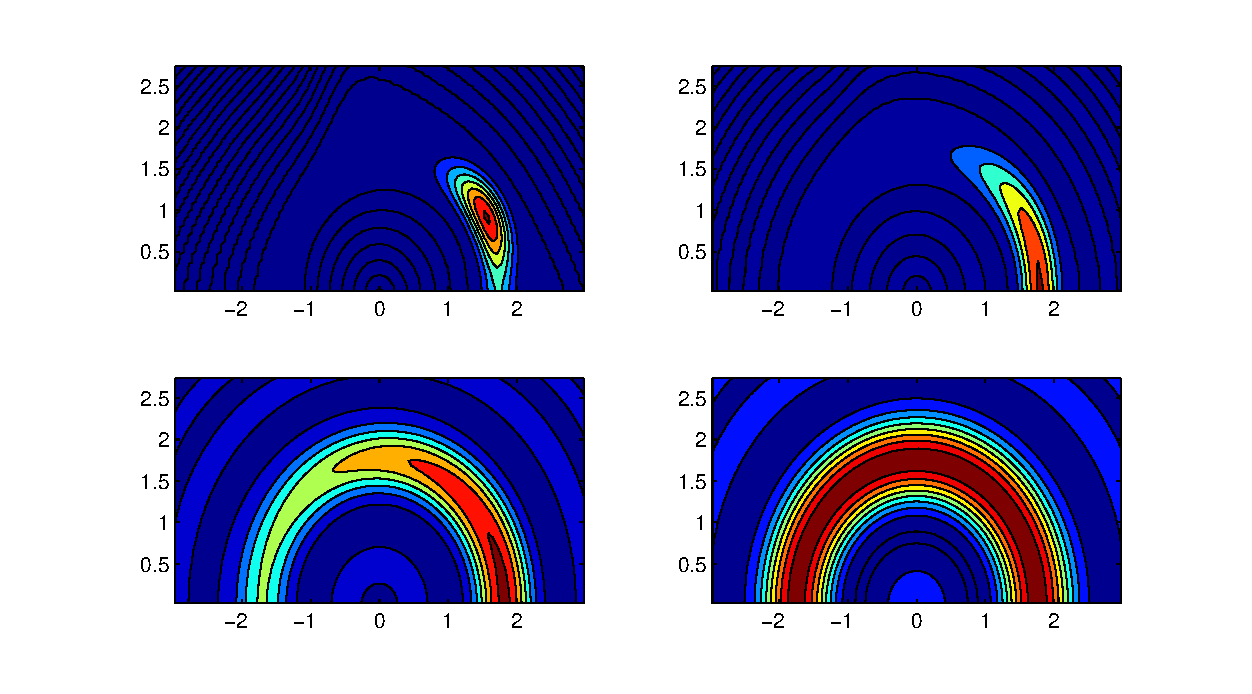
\includegraphics[width=0.6\textwidth]{pitchangle.eps}
\caption{Snapshot of velocity space as three different time intervals showing the effect of pitch angle scattering on the velocity space.  Coordinates are $v_{\parallel}$ horizontally and $v_{\perp}$ vertically. All data shown in this chapter was run with 100 parallel velocity points and 50 $\mu$ points non-equally spaced.\label{pitch-angle}}
\end{center}
\end{figure}

\subsection{Energy scattering}

This effect is switched on by setting \name{en_scatter} $=$ \name{.true.} in the collisions input deck.  The energy scattering term spreads the distribution function in energy.

\subsection{Collisional friction}

This effect is switched on by setting \name{friction_coll} $=$ \name{.true.} in the collisions input deck.  The collisional friction term advects the distribution function towards the origin in velocity space.

When you combine all three effects we get an evolution of the distribution function towards a Maxwellian centred on zero and with a width of a single normalised thermal velocity.

\begin{figure}
\begin{center}
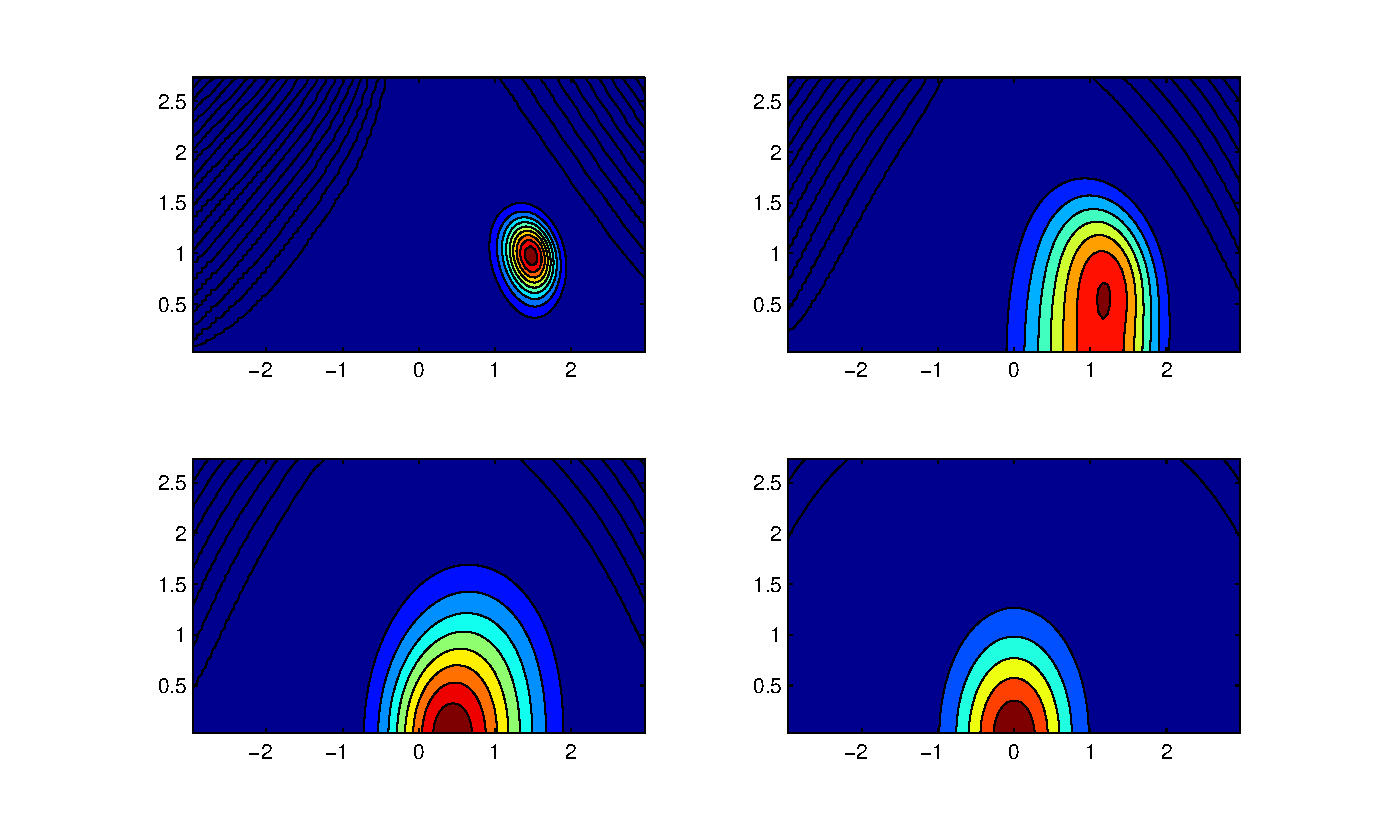
\includegraphics[width=0.6\textwidth]{fulloper.eps}
\caption{Snapshot of velocity space as four different time intervals showing the effect of all the terms in the collision operator on the velocity space.  The final state is a Maxwellian centred on zero.}
\end{center}
\end{figure}

\begin{figure}
\begin{center}
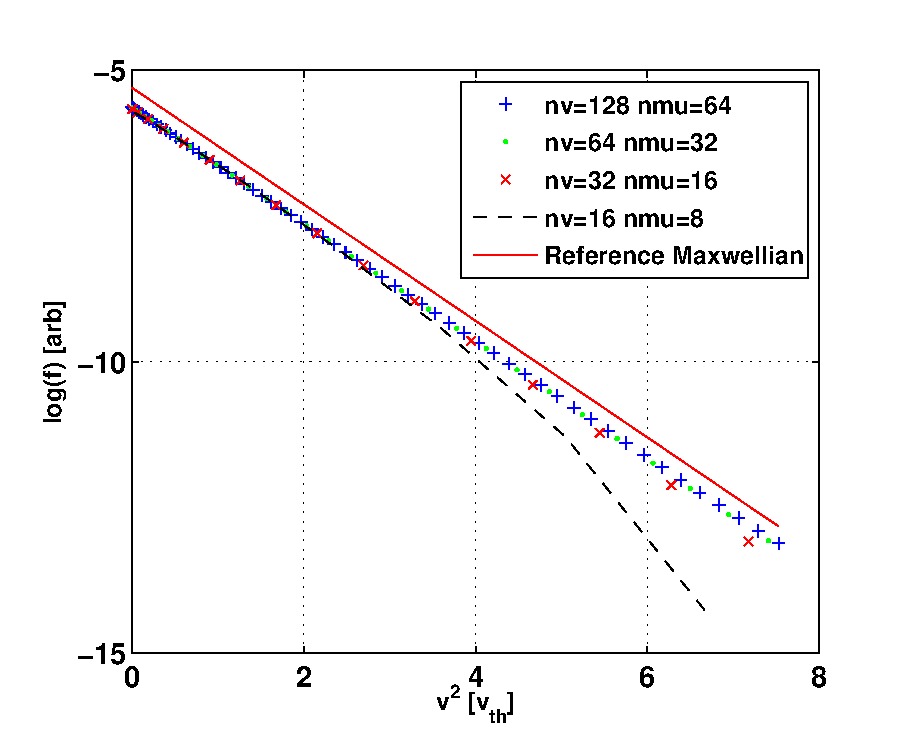
\includegraphics[width=0.65\textwidth]{../benchmarks/collisions/CollisionsMaxwellian.eps}
\caption{Figure showing the logarithm of the distribution function as a function of $v^2$ for varying velocity space resolutions.  A reference 
Maxwellian is also plotted for comparison.}
\label{maxwellcoll}
\end{center}
\end{figure}


\section{Velocity space boundary conditions}

There are currently two options for the boundary conditions in velocity space.  The input deck parameter \name{mass_conserve} changes between open boundary conditions (when set to \texttt{.false.}, default) and zero flux boundary conditions (when set to \texttt{.true.}).  The former is more physical, but the latter is useful for testing of conservation properties to machine precision. The difference in mass conservation between the two is very small.
\begin{figure}
\begin{center}
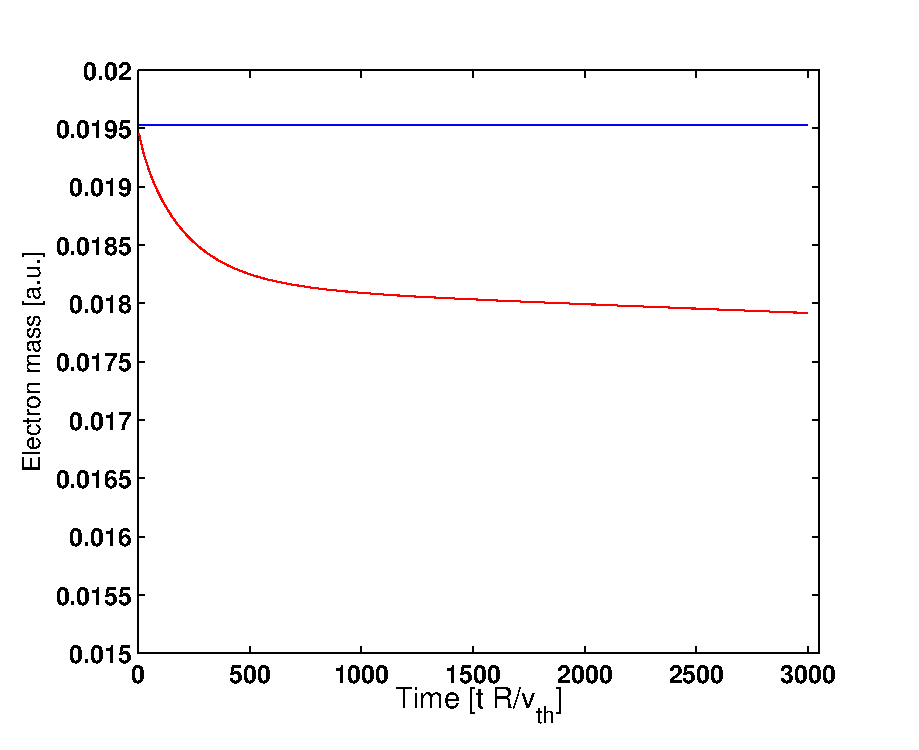
\includegraphics[width=0.45\textwidth]{../benchmarks/collisions/MassConservation.eps}
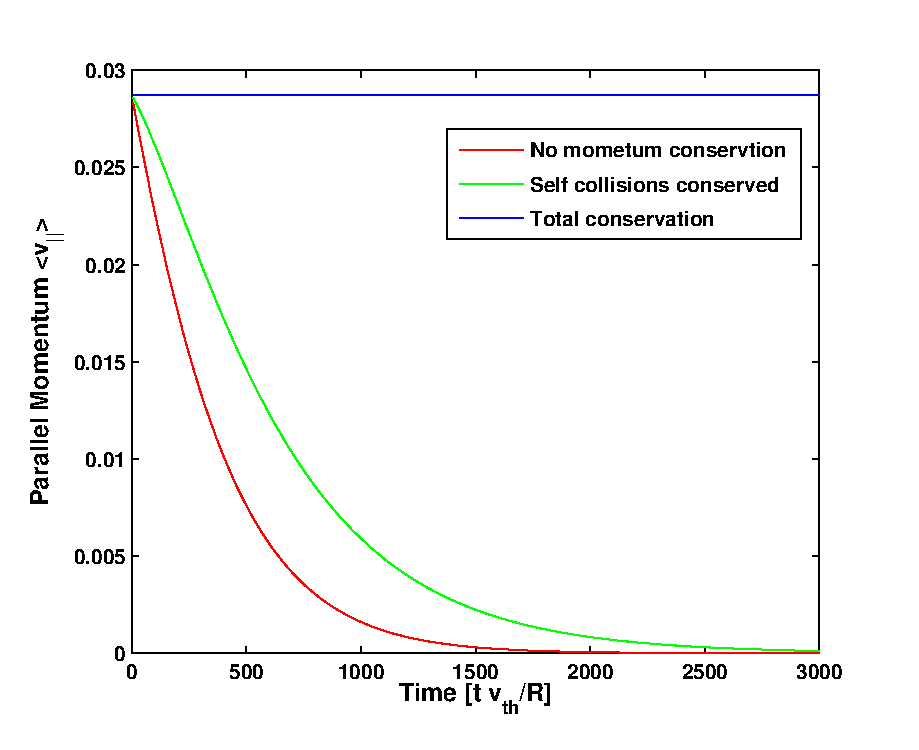
\includegraphics[width=0.45\textwidth]{../benchmarks/collisions/MomentumCons.eps}
\caption{(left) Figure shows the electron particle mass for when (blue) flux conserving boundaries and (red) open boundaries are used.  When the former is chosen the particle number is conserved to machine precision.  
Note the y-axis scale.  (Right) Shows the parallel momentum for runs with the same initial conditions for (blue) fully conservative (green) self collisions conservative
and (red) no conservation at all.  Again, the momentum is conserved to machine precision.  }
\end{center}
\end{figure}

\begin{figure}
\begin{center}
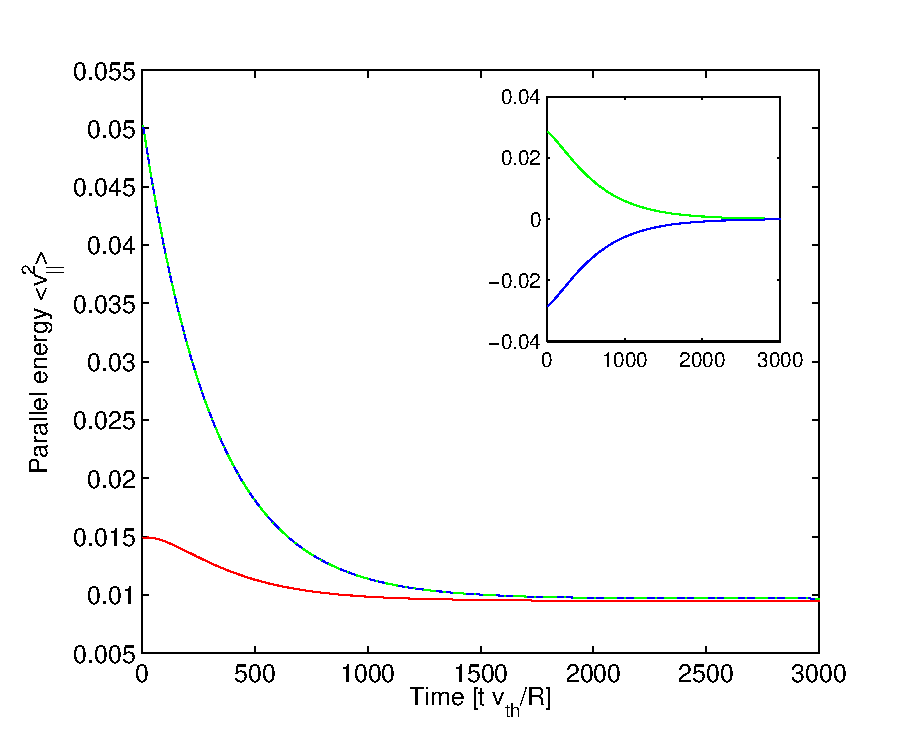
\includegraphics[width=0.5\textwidth]{../benchmarks/collisions/EnergyConvergence.eps}
\caption{Figure shows the energy in the electron distribution for three different initial conditions (green and blue had the same initial width but with a different parallel velocity sign, red was gaussian centered different initial parallel velocity).  
All three converge on the same value. (Inlay is the parallel momentum)}
\end{center}
\end{figure}

\section{User defined collision-frequencies}

The collision frequency can be defined in two ways.  Firstly by specifying \name{nref} which is the particle density in units of $10^{19}$ particles per $m^{3}$, \name{tref}, the temperature in keV and \name{rref} which is the toroidal major radius.  These parameters are what the corresponding parameters are normalised to in the code and are never usually specified.  The normalised collision frequency $\Gamma^{a/b}=\nu_{ab} R_{\rm ref}/v_{\rm tha}$ is given by,

\begin{equation} 
\Gamma^{a/b}_N = {R_{\rm ref} n_b Z_a^2 Z_b^2 e^4 \ln \Lambda^{a/b} \over 4 \pi \epsilon_0^2 m_a^2 v_{tha}^4} = 
6.5141\cdot 10^{-5} {R_{\rm ref} n_{\rm ref}^{19} \over (T_{\rm ref}^k)^2}  {n_{Rb} Z_a^2 Z_b^2 Z^{a/b}_{\rm eff}\ln \Lambda^{a/b} 
\over T_{Ra}^2}
\end{equation}
where $Z^{a/b}_{\rm eff} = 1.0 $ unless $b = i$ (main ion species) as determined by the species density and $a = e$ as determined by the charge on the species.
The value of $Z^{e/i}_{\rm eff}$ is adjusted by the parameter \name{zeff} in the collisions namelist which is 1.0 by default. 
Note that if impurity species are included kinetically, then the scaling factor will be automatically modified to be 
\begin{equation}
 Z^{e/i}_{\rm eff} = 1 + (\name{zeff} - Z_\textrm{eff}^\textrm{sp})\frac{n_e}{n_iZ_i^2}
\end{equation}
with $Z_\textrm{eff}^\textrm{sp}=\frac{1}{n_e}\sum_s n_sZ_s^2$ and the sum on 's' performed on all ion species

However if \name{freq_override} $=$ \texttt{.true.} then,

\begin{equation}
\Gamma^{a/b}_N =  Z_a^2 Z_b^2 \nu_{\rm ref} \frac{n_{Rb}}{T_{Ra}^2} \frac{\ln \Lambda^{a/b}}{\ln \Lambda^{i/i}}
\end{equation}

Where $\nu_{\rm ref}$ is the user defined frequency defined as \name{coll_freq} in the input deck.  This is assumed to be the singly charged ion - ion (proton or deuteron) collision frequency.  To get agreement with the first method this can be set to $6.5141\cdot 10^{-5}R_{\rm ref}n_{\rm ref}^{19}\ln \Lambda^{i/i}/(T_{\rm ref}^k)^2$.  This value is then scaled to all the other species respectively.  For this to work the first species in the input deck should be singly charged ions.

\section{Direct benchmarks}

Here outlined is a direct analytical benchmark of the collision operator. The frictional slowing down of a particle can be calculated 
analytically, and accuratly approximated in the code by using a very narrow, high energy gaussian in velocity space.  The velocity
of this pulse can then be tracked and compared with the analytic expression.

The slowing down time of a particle can be written as:
\begin{equation}
\tau^{s} = - \frac{U}{\frac{\partial U}{\partial t}}
\end{equation}
where $\tau^{s} = 1/\nu_{S}$, which is defined as (we consider only ion-ion collisions):

\begin{equation}
\nu^{a/b}_{S} = - \left[ (1 + \frac{m_{a}}{m_{b}})\psi(x)\right]\nu_{0}^{a/b}
\end{equation}
where $\nu_{0}^{a/b}=\Gamma^{a/b}_N = {R_{\rm ref} n_b Z_a^2 Z_b^2 e^4 \ln \Lambda^{a/b} \over 4 \pi \epsilon_0^2 m_a^2 v_{a}^3} $,
where $\psi(x)$ is the Maxwell integral and can be shown to be $\psi(x) = erf(x) - x \frac{\partial erf(x)}{\partial x}$.  
and x is defined as $v^{a}/v_{th}^{b}$.  This ordinary differential equation can then be solved using standard methods.  The comparison between
GKW and this result is shown in Fig.~\ref{slowdown}.
\begin{figure}[h!]
\begin{center}
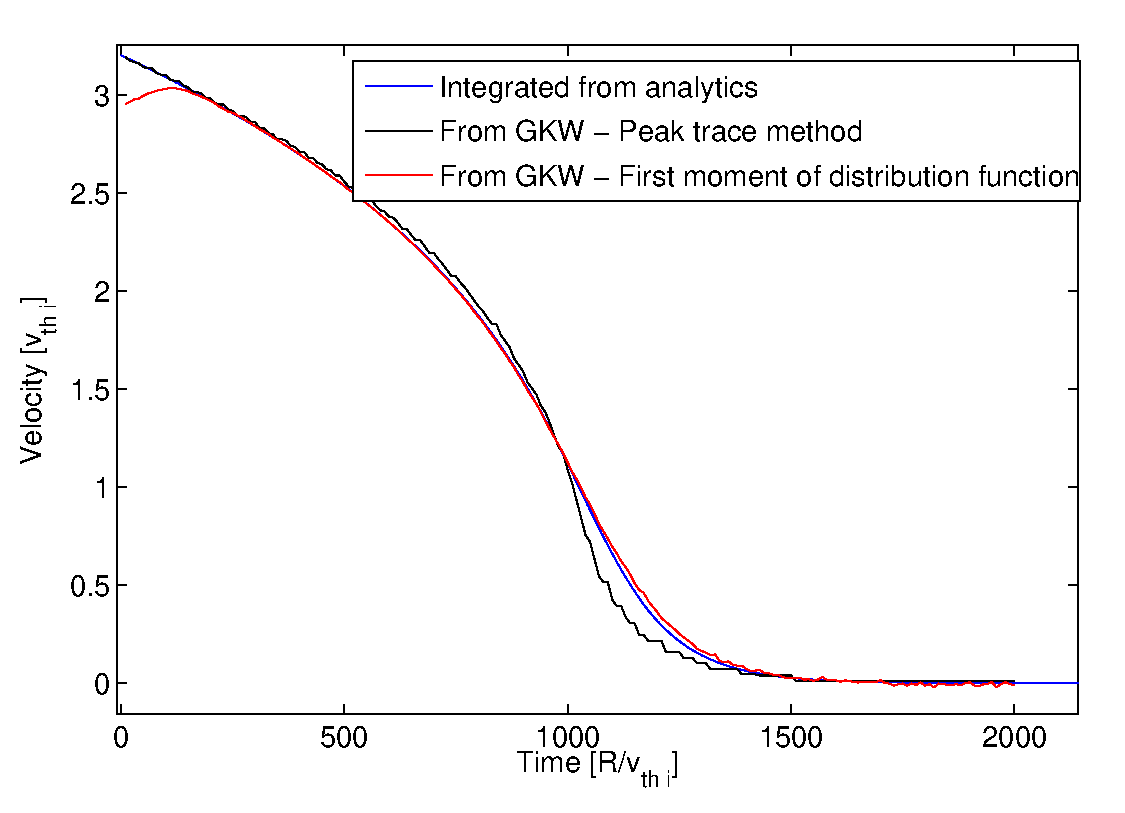
\includegraphics[width=0.60\textwidth]{../benchmarks/collisions/SlowingDownComparison2.eps}
\caption{Measurement of the velocity of a highly localised pulse in velocity space as a function of time.  The result from GKW is shown
utilising two methods, one is the first moment of the distribution function, while the other is simply a trace of the spike.  The blue line is 
the solution of the ODE described above.}
\label{slowdown}
\end{center}
\end{figure} 
Agreement between the two curves is very good, implying that the friction and energy scatter terms are operating correctly
in the current implementation.  A benchmark of the pitch angle scattering against another code is presented in Sec. \ref{linearbenchmarks}.

% related to auctex mode and latex-preview-mode in Emacs:
%%% Local Variables:
%%% mode: latex
%%% TeX-master: "doc"
%%% End:

\chapter{Rotation and poloidal asymmetries}

The co-moving system employed in GKW corresponds to a frame that rotates as a rigid body with constant frequency 
$\Omega$. The Coriolis drift, centrifugal drift, centrifugal trapping and centrifugal potential 
due to the rotation of the plasma are all incorporated in the complete set of equations described above. 
The possible radial gradient in the toroidal rotation is  treated through a radial gradient in the averaged parallel velocity $u^\prime$ 
of the background.  The radial gradient of the perpendicular velocity ($E \times B$ shear flow) has so far been ignored, 
but is known to play an important role in the saturation of the turbulence.  

In this chapter we describe how the centrifugal potential is calculated from the species inputs, 
and how the  the $E \times B$ shearing is treated in GKW.  Much of this Chapter appears in greater detail in Ref. \cite{Casson-Thesis}.

%Describe further:
% Origin of cf potential
% Why some terms vd.grad remain and others not from ordering.
% Maxwellian
% Make note in arawaka scheme about s periodicity.
% Modification to collisions
% Choice of n_{R_0 location}
% Feild equations do not need modifying
% deriv wrt zeta zero due to axisymmetry

%Do
%Check Arakawa scheme is working correctly with mode_box

%Discuss
% No gyroaverage of phi


\section{Centrifugal potential\label{cfphi}}
We recall that the rotation of the plasma leads to an equilibrium density variation within a flux surface
\begin{equation}
  n(s)=n_{R_0,s} \exp\left({-Z_s \langle\Phi\rangle\over T_{R,s}}+{m_s\Omega^2(R^2-R_0^2)\over T_{R,s}}\right) 
\end{equation}
(normalised units). The background equilibrium potential $\Phi$ in the rotating frame is found by applying the quasi-neutrality condition over all the species
\begin{equation}
  Q(\Phi)=\sum_s Z_s n_{R_0,s} \exp\left({-Z_s \langle\Phi\rangle\over T_{R,s}}\right)\exp\left({m_s\Omega^2(R^2-R_0^2)\over T_{R,s}}\right)=0
  \label{eq:cf-quasineutral}
\end{equation}
Since there is only one negative species and the exponential function is monotonically increasing, the equation $Q(\Phi)=0$ will always have exactly one root.  
In GKW, $\Phi$ is calculated numerically for arbitrary species combinations from the quasi-neutrality condition by an iterative root finding bisection algorithm.  The calculation is done once for each point in $s$ during the initialisation phase of the code. 
The terms II, VI, and VIII (\ref{eq:II}, \ref{eq:VI}, \ref{eq:VIII}) also require the $\psi$ and $s$ derivatives of $\Phi$, which are calculated using a fourth-order finite difference.

%Describe bisection method
The bisection algorithm begins with an upper limit estimate $\Phi_a$ for $\Phi$.  The initial value used in GKW is (somewhat arbitrarily) taken as
\begin{equation}
  \biggr[\max\{\log(1+|Z_s n_s|)\}+\max\{m_s\log(1+n_s)\}\biggr]\Omega^2 (R^2-R_0^2) + 0.1
\end{equation}
which should always contain the root, but be small enough to prevent exponentiation overflows.  It is possible that extreme
species input data could break the solver, and the upper limit estimate might need to be adjusted for those cases.
% The earlier condition below caused an overflow for tungsten impurities:
% \begin{equation}
% \Phi_a = 5\max(T_s)\left[\log\left(\left|{\max(Z_s)\max(m_s) \over \min(T_s)}\right|\right)+\log\left(|\Omega^2(R^2-R_0^2)|\right)\right]+0.1
% \end{equation}

The starting lower limit is estimated as $\Phi_b=-\Phi_a$. The value is chosen to ensure that the root lies in the range $(\Phi_b,\Phi_a)$. In each step the mid value $\Phi_{\rm est}=(\Phi_a+\Phi_b)/2$ is taken and the value of $Q(\Phi_{\rm est})$ is calculated.  If $Q(\Phi_{\rm est})>0$, then the upper estimate is updated ($\Phi_a=\Phi_{\rm est}$), and if $Q(\Phi_{\rm est})<0$, then the lower estimate is updated ($\Phi_b=\Phi_{\rm est}$).  The process repeats until the solution has converged to within machine accuracy.  The bisection algorithm, while not the fastest possible, is guaranteed to converge as long as the bounds are appropriate and the function $Q$ has only one root in the initial range.  In practice, the convergence occurs in about 55 iterations using the initial estimates specified above.  The function $Q(\Phi,s,\psi)$ is evaluated in module \name{components} as \name{cf_quasineutral} called from the bisection algorithm \name{centrifugal_energy} in module \name{rotation}.

In the local flux tube model, the gyrokinetic equation is solved only on one flux surface (i.e. at one position in $\psi$), keeping radial derivatives of equilibrium quantities.  To consistently calculate the radial derivative of $\Phi$, equation \ref{eq:cf-quasineutral} is also solved numerically on adjacent flux surfaces using $Q(\Phi,s,\psi+\Delta \psi)$, using the radial derivatives of the species quantities to calculate the temperature and densities on adjacent flux surfaces.

The choice of $\Delta \psi$ used in the code is motivated by a compromise between machine precision when dividing by small numbers, and the accuracy of the finite difference as $\Delta \psi \rightarrow 0$.  The discrepancy between the root finding algorithm and the analytic solution (Eq. \ref{eq:deriv-scions}) is plotted in figure \ref{fig:cfphi-acc}. The value of $\Delta \psi = 1e-4$ is implemented as a permanent choice, which for the case investigated minimises the error to less than $10^{-11}$ in double precision.

\begin{figure}
\begin{center}
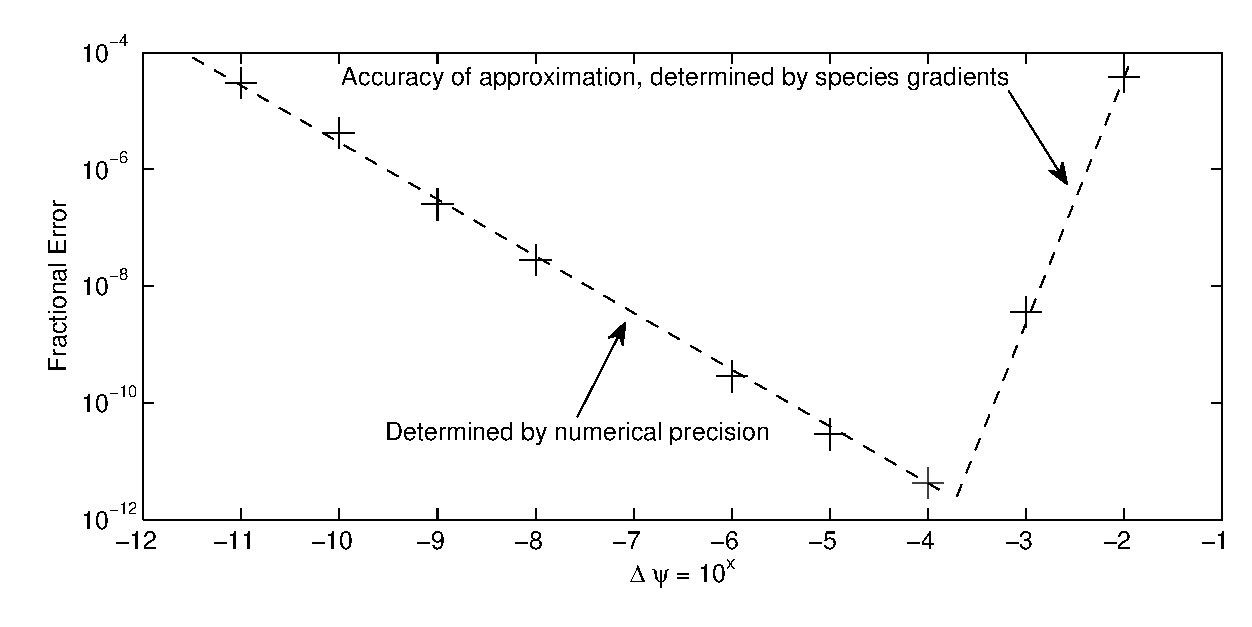
\includegraphics[width=0.6\textwidth]{cfphi-accuracy.eps}
\caption{Numerical experiment to determine optimum $\Delta \psi$ for calculating the radial derivative of the centrifugal potential $\Phi$ for the singly charged ions Waltz standard case. The experiment was conducted in double precision and the fractional error is calculated against the analytic result Eq. \ref{eq:deriv-scions}.}

\label{fig:cfphi-acc}
\end{center}
\end{figure}

In the case of a plasma of only singly charged ions, Eq. \ref{eq:cf-quasineutral} solves exactly to give
\begin{equation}
 \Phi = \underbrace{{T_e T_i \over T_e + T_i} \left({m_i \over T_i} - {m_e \over T_e}\right)}_{\name{cf_mass_weight}} \Omega^2 (R^2-R_0^2).
\label{eq:scions}
\end{equation}
with radial derivative 
\begin{equation}
 {\partial \Phi \over \partial \psi} = \underbrace{\left[{m_i {\partial T_e \over \partial \psi}- m_e {\partial T_i \over \partial \psi}\over T_e + T_i} + 
{m_e T_i - m_i T_e \over (T_e + T_i)^2}\left({\partial T_e \over \partial \psi}+{\partial T_i \over \partial \psi}\right)\right]}_{\name{cf_dtf1}}\Omega^2(R^2-R_0^2) 
+2 \Omega^2 \underbrace{\left[{m_i T_e - m_e T_i \over T_e + T_i}\right]}_{\name{cf_mass_weight}} 
\left(R {\partial R \over \partial \psi}-R_0 {\partial R_0 \over \partial \psi}\right)
\label{eq:deriv-scions}
\end{equation}
%ADD UPRIME PIECE HERE, and in COMPLETE SET OF EQUATIONS, and in solver above
If the bulk ion species is singly charged, these quantities are evaluated in the code in \name{rotation} with the labelled function provided by \name{components} to provide a check on the solution of the root finding algorithm.  

The density $n_R$ and density gradient $1/L_n=(1 / L_n)_{R_0}$ (Eq. \ref{eq:gradients}) are defined for each species at the point on the flux surface at which $R=R_0$.  Two choices for the definition of $R_0$ are available in the code, which are selected by the input variable \name{R0\_loc} in the \name{geom} namelist.  The option \texttt{R0\_loc='axis'} sets $R_0$ as the major radius of the magnetic axis (but the reference point is not on the axis itself), whilst the default \texttt{R0_loc='LFS'} sets $R_0$ to be the value of $R$ at $s=0$, in the plane of the magnetic axis at the low field side (for general geometry this may \textit{not} be equivalent to the maximum $R$).  This choice alters only the definition of the geometry quantities $\mathcal{J}$ and $\mathcal{K}$ .  In the rotating case, the effective density gradient varies over the flux surface and there is no longer one obvious definition of the density gradient as a dimensionless quantity.  For instance
\begin{equation}
{1 \over L_n^{E} } = -{1 \over n} {\partial n \over \partial \psi},\qquad
{1 \over L_n^{e1} } = -{1 \over \{ n \} } {\partial n \over \partial \psi},\qquad
{1 \over L_n^{e2} } = -{1 \over n_{R_0}} {\partial n \over \partial \psi}, \qquad
\label{eq.rlndiags}
\end{equation}
can each be argued to be a relevant quantity. The most appropriate may be determined by the nature of the particular instability being examined. These definitions can be evaluated to be

\begin{equation}
{1 \over L_n^{e} } = {\partial \cfenn \over \partial \psi} + 
\cfenn {1 \over L_T}+  {1 \over L_n} \biggr|_{R_0}, \qquad
{1 \over L_n^{e1} } = {1 \over L_n^{e} } { \exp(-\cfenn) \over
\big\{ \exp(-\cfenn) \big\} }, \qquad
{1 \over L_n^{e2} } = {1 \over L_n^{e} }  \exp(-\cfenn)
\label{eq.rlndiags2}
\end{equation}

Since the density gradient is an important parameter for determining the stability of many modes, GKW calculates ${1 / L^E_N }$ and ${1 / L^{e1}_n }$ and $n/n_{R_0}$ for each species as a function along the field, which is written to the file \File{cfdens.dat}, and as
a flux surface average and at the outboard midplane, which is written to screen during the initialisation phase of the code. ${1 / L^{e2}_n }$ can be trivially calculated from the other two.  It should be noted that whilst the input ${1 / L_n} |_{R_0}$ must always be the same for every species in order to satisfy quasi-neutrality, the effective  ${1 / L_n^E}$ can differ for each species.  For typical parameters of a deuterium plasma, the variation in effective density and gradient can be $30\%$ at $\Omega=1$, increasing rapidly for $\Omega>1$.

\section{Background \texorpdfstring{$E \times B$}{E x B} shear flow}

The sheared $E\times B$ velocity leads to a stabilisation of turbulence through the breaking up of eddy structures. 
This $E\times B$ shearing is always present for a purely toroidally rotating plasma but can, of course, also be related 
to a sheared poloidal rotation. 

%FJC: CHECK AGAIN FACTORS OF RHO* What happens if normalise as background potential?

The equilibrium $E \times B$ rotation 
\begin{equation}
{\bf v}_s(\psi)= {{\bf b} \times \nabla \bar{\Phi} \over B} 
\end{equation}
lies inside the flux surface.  The shearing rate in the normalised units is defined to be 
\begin{equation}
\gamma_{E}^N = {1 \over 2}\rho_*^2 {\partial^2 \bar{\Phi}_N \over \partial \psi^2} ,
\label{gamma-E}
\end{equation}
where the normalisation $\bar{\Phi}= \rho_* {T_{\rm ref} \over e}\bar{\Phi}_N$ is as for the
perturbed potential Eq.~(\ref{eq:phi-norm}).  The factor $1/2$ is present due to the definition of the
reference thermal velocity.  Since GKW treats the $E \times B$ shear independently from the centrifugal effects,
we use $\bar{\Phi}$ to distinguish the background potential of the shearing from the background potential of the rotating frame.
In physical units the shearing rate is
\begin{equation}
\gamma_E = {v_{\rm thref} \over R_{\rm ref}} \gamma_E^N = 
{1 \over B_{\rm ref}}{\partial^2 \bar{\Phi} \over \partial r^2} ,
%Contingent on \phi=r/R_{ref}
%True if r = R_{max}-R_{min}
\end{equation}
where $r=(R_{\rm max}-R_{\rm min})/2$.  The GKW shearing rate is assumed
radially constant and is defined as a flux function.  At the radial centre of the flux tube
$\bf{v_s}$ is chosen to be zero, with the result that there is no net flow over the domain.  In the
local limit with the approximations of the `$s-\alpha$' model geometry
the shearing rate is then equivalent to the familiar definition \cite{Hahm95,Burrell97}:
\begin{equation}
\gamma_E \approx {(RB_p)^2 \over B_t}{\partial^2 \bar{\Phi} \over \partial \Psi^2}
\approx {d v_s \over d r} .
\end{equation}
The flow velocity is normalised as $v_s^N=v_s / v_{\rm thref}$, and as before the index $N$ is dropped in what follows.
The sign convention here is opposite to Eq.~(\ref{eq:gradients}), so $\gamma_E<0$ corresponds to 
$\nabla E_0$ radially outwards.

Only the Doppler shift of the background $E \times B$ rotation is kept in the description, i.e. the
background $E\times B$ rotation is 
added as an additional convective term for the perturbed distribution (${\bf v}_s \cdot \nabla g$) in the gyrokinetic equation~(\ref{eqs:complete-set}), 
and we neglect the acceleration due to the background potential (${\bf v}_D \cdot \nabla \bar{\phi} F_M$). 
By omitting the latter term, the flow is implemented in conservative form and provides no drive to the turbulence, so that the 
stabilising effect may be studied in isolation.  If the acceleration term were kept, it would provide a Kelvin-Helmholtz drive to
the turbulence.  This drive is likely to be small compared to the parallel shear drive (which is kept in term VIII), but could be the subject of future work. 

With zero net flow across the flux tube one obtains
\begin{equation}
{\rm III.B} = -{\bf v}_s \cdot \nabla g \rightharpoonup - \rho_*^2 {\partial \bar{\Phi} \over \partial
\psi}{\mathcal E}^{\psi \zeta}{\partial g \over \partial \zeta} =
 - 2 {\gamma_E \psi}{\mathcal E}^{\psi \zeta}  {\partial g \over \partial \zeta} .
\end{equation}
Defining $\bar \gamma_E= 2 \gamma_E {\mathcal E}^{\psi \zeta} $ and taking the Fourier transform, the term can be written as a derivative in
Fourier space
\begin{equation} 
{\mathcal T}(-{\bar \gamma_E \psi}{\partial g \over \partial \zeta}) = \bar \gamma_E
k_\zeta {\partial \hat g \over \partial k_\psi} .
\end{equation}
The derivative represents a continuous advection (and shearing) in Fourier space in $k_\psi$.  

There are a number of subtleties associated with numerical evaluation of this derivative. A finite difference approximation cannot resolve the fine 
scale structure in Fourier space.  The `harmonic derivative' \cite{Waltz94,Miller94} is a full convolution over all modes and is equivalent to a
pseudo-spectral implementation using FFTs (as was used for the nonlinear term in Eq.~(\ref{eq:nl-term})).  
Although it correctly implements the $E \times B$ shearing term inside the computational domain, it does not represent a homogeneous shear 
flow because the flow profile does not satisfy the periodicity of the discrete Fourier transform; any turbulent structure passing through the radial
boundary will experience a discontinuity in the flow profile (which in the periodic domain has a sawtooth form).  
Since the local limit requires that the turbulence has no preference for the boundary, periodicity at the boundary must be preserved. 
The `shear-periodic' boundary condition \cite{Baron82,Schumann85,Gerz89} that moves with the mean flow accomplishes this for a finite 
difference representation in the radial direction, but does not naturally translate to the spectral representation.

In coordinates that move with the flow  \cite{Rogallo81,Zang88,Pumir96}, the `radial' wavenumbers become time dependent:
\begin{align}
\psi^\prime = \psi , &\qquad& \qquad \zeta^\prime=\zeta-\psi \bar \gamma_E t ,\\
k_\zeta^\prime = k_\zeta , &\qquad& \qquad  k_\psi^\prime = k_\psi - k_\zeta \bar \gamma_E t .
\end{align}
In these coordinates, the derivative in Fourier space becomes part of the time derivative.

For a gyrokinetic code, a time dependent wave vector requires the re-evaluation of the linear terms and Bessel functions at every time-step
and would be computationally prohibitive. 
By discretising the time dependence of the wavenumbers as a remapping of the solution vector between the original fixed wavevectors, 
this expensive re-evaluation can be avoided \cite{HammettAPS06}. 
Using only the fixed wavevector grid, the advection in Fourier space occurs in jumps only when the boundary periodicity is satisfied for a 
given mode. 
Explicitly, the remapping is implemented by tracking the number of times each wavevector has been remapped $i_r(k_\zeta)$, 
and (for $\bar{\gamma}_E > 0$) remapping the solution vector
\begin{equation}
\hat g (k_\psi, k_\zeta,s) \rightarrow \hat g (k_\psi-\Delta k_\psi, k_\zeta,s),
\end{equation}
 when the inequality
\begin{equation}
 {\rm Int}( k_\zeta \bar{\gamma}_E t / \delta k_\psi ) > i_r (k_\zeta),
\end{equation} 
is satisfied.  Here, ${\rm Int}$ is the function which returns the \textit{nearest} integer.
At the low $k_\psi$ limit the solution vector is discarded.  
This means that the method is non-conservative, but since the turbulence is characterised by a peaked spectrum 
(Fig.~\ref{fig:cyclone-linear}), the losses are negligible if the range of radial wavenumbers is suitably wide.  
For numerical stability, the remapping must occur at the same time for all points along the flux tube. 
As the metric tensor ${\mathcal E}^{\psi \zeta}$ is a flux function, see Eq.~(\ref{eq:efun-cst}), this condition is always satisfied for a 
constant shear rate along the field line.

The method in GKW differs from the standard spectral methods to model homogeneous shear flows in fluid turbulence of
Refs.~\cite{Rogallo81,Zang88,Pumir96}, where the wavenumbers must be recalculated and re-meshing occurs for all wavevectors 
at the same time. 
In GKW the method used is the one proposed by Hammett et al. in Ref.~\cite{HammettAPS06}.  
Here the `re-meshing' occurs continually (and at different times for each $k_\zeta$), and the wavenumbers stay on their original fixed grid.  
The accuracy of the method has been argued to be second order on average \cite{HammettAPS06} and
is able to capture the physics effects of a 
background shear flow whilst allowing the desirable features of the flux tube model to be retained.
 
Convergence of the remap method in $L_x / L_y$ should be checked (particularly by for the modes with lowest $k_\zeta$) by decreasing 
$\Delta k_\psi / k_{\zeta {\rm min}}$ (increasing $N_x$ and $p$ (IKXSPACE) whilst holding $N_{\rm mod}$ constant (defined later)).


\section{Purely toroidal sheared rotation in general geometry}

For this section only, we adopt the superscript $^L$ to represent quantities in the laboratory frame.  
All quantities without a superscript should be interpreted as being in the rotating frame (as in all other sections). 
The same coupling condition is derived by two routes to make clear the relationship between the frames.

The rotating frame is constructed \cite{PEE09} such that rigid body rotation $\Omega$ of the frame 
matches the plasma rotation $\omega_\phi^L$ on the local flux surface.  The angular rotation then transforms
as 
\begin{equation}
\omega_{\phi}(\psi)=\omega_{\phi}^L(\psi)-\Omega 
\label{eq:transform}
\end{equation}
such that $\omega_{\phi}(\psi)=0$ (and hence ${\bf
v_s}=0$) at the centre of the radial domain. 

\subsection{In comoving frame}

For a purely toroidal rotation, decomposing the toroidal flow into its parallel and perpendicular components gives
\begin{equation}
u_\parallel \mathbf{b} +  \mathbf{v_s} = s_{\rm B} R \omega_\phi(\psi) R \nabla \varphi,
\label{eq:toroidal}
\end{equation}
where $\varphi$ is the toroidal angle. Since \eq{toroidal} is written in the comoving frame,
 it reads $0+0=0$ in the centre of the flux tube.
From the normalisations above, one can show that in the normalised units
\begin{equation}
 \mathbf{v_s} = {1 \over 2} \rho_*^2 {\mathbf{b} \times \nabla \psi \over
B} {\partial \bar{\Phi} \over \partial \psi}.
\end{equation}
Taking the bi-normal component of \eq{toroidal} one finds
\begin{equation}
 u_{\parallel} \underbrace{\mathbf{b} \cdot \nabla \zeta}_{=0} +  {1 \over 2}
\rho_*^2 \underbrace{{\mathbf{b} \times \nabla \psi \over B}\cdot \nabla
	\zeta}_{=2\mathcal{E}^{\psi \zeta}}{\partial \bar{\Phi} \over \partial \psi} = s_{\rm B} R^2 \omega_{\phi}(\psi)
\underbrace{\nabla \phi \cdot \nabla \zeta}_{=-1/2\pi R^2},
\end{equation}
hence
\begin{equation}
 {1 \over 2} \rho_*^2 {\partial \bar{\Phi} \over \partial \psi} = - {s_{\rm B} \over 4 \pi}{1 \over
\mathcal{E}^{\psi \zeta}}\omega_{\phi}(\psi),
\label{eq:comoving}
\end{equation}
which upon differentiation gives the coupling relation
\begin{equation}
 \underbrace{{1 \over 2} \rho_*^2 {\partial^2 \bar{\Phi} \over \partial \psi^2}}_{\gamma_E} = - {s_{\rm B} \over 4 \pi}\left[{1 \over
\mathcal{E}^{\psi \zeta}}\underbrace{\partial \omega_{\phi} \over \partial \psi}_{\rm u^\prime} +
\underbrace{\omega_\phi}_{=0}{\partial \over \partial \psi} \left({1 \over \mathcal{E}^{\psi \zeta}}\right)\right].
\label{eq:coupling}
\end{equation}
Note that the second term on the right is zero when evaluated at the centre of the flux tube.
All quantities in the above equation are flux functions, hence the shear rate will always be a
flux function, as required for the discrete remapping method.


\subsection{Relation to lab frame}

In the laboratory frame \eq{toroidal} becomes 
\begin{equation}
u_\parallel^L \vec{b} + {\bf v}_s^L  = s_{\rm B} R \omega_\phi^L(\psi) R \nabla \varphi.
\label{eq:toroidal2}
\end{equation}
Taking the binormal component leads to
\begin{equation}
 {1 \over 2} \rho_*^2 {\partial \bar{\Phi}^L \over \partial \psi} = - {s_{\rm B} \over 4 \pi}{1 \over
\mathcal{E}^{\psi \zeta}}\omega^L_{\phi}(\psi),
\end{equation}
and taking the radial derivative gives
\begin{equation}
 {1 \over 2} \rho_*^2 {\partial^2 \bar{\Phi}^L \over \partial \psi^2} = - {s_{\rm B} \over 4 \pi}\left[{1 \over
\mathcal{E}^{\psi \zeta}}{\partial \omega^L_{\phi} \over \partial \psi} + \omega^L_{\phi}{\partial \over \partial
\psi} \left({1 \over \mathcal{E}^{\psi \zeta}}\right)\right],
\end{equation}
which has the same form as \eq{coupling} but different values.

To make explicit the relationships between the quantities, the previous equation 
is rewritten (using \eq{transform}) in terms of the rotating frame quantities.
Since the frame rotates rigidly, ${\partial \Omega \over
\partial \psi}=0$ and ${\partial \omega / \partial \psi} = {\partial \omega^L / \partial \psi} = u^\prime$. 
The tensor component $\mathcal{E}^{\psi \zeta}$ is invariant under the transformation.
The electric field transforms \cite{PEE09} as
\begin{equation}
\bar{\Phi}=\bar{\Phi}^L + s_{\rm B} s_{\rm j}{2 \over \rho_*^2}\Psi \Omega ,
\end{equation}
where $\Psi$ is the (frame independent) poloidal flux with $\nabla \Psi$ radially outward, 
and the factor of $2 / \rho_*^2$ arises from the normalisation of $\bar{\Phi}$ (see Sec. \ref{signs} for clarification of signs).  
The coupling condition can then be written as 
\begin{equation}
 \underbrace{{1 \over 2} \rho_*^2 {\partial^2 \bar{\Phi} \over \partial \psi^2}
-s_{\rm B} s_{\rm j}  {\Omega}{\partial^2 \Psi \over
\partial \psi^2}}_{\gamma_E^L} = - {s_{\rm B} \over 4 \pi}\left[{1 \over
\mathcal{E}^{\psi \zeta}}{\partial \omega_{\phi} \over \partial \psi} +
\Omega{\partial \over \partial \psi} \left({1 \over \mathcal{E}^{\psi \zeta}}\right)\right],
\end{equation}
when evaluated in the centre of the flux tube where $\omega_\psi = 0$.
Since $\Psi=f(\psi)$ only, from the relation \ref{eq:efun-flux}
% \begin{equation} 
% {\cal E}^{\psi \zeta} = \frac{s_{\rm j}}{4\pi}\frac{\partial \psi}{\partial \Psi}
% \label{eq:efun-cst}
% \end{equation}
it follows that
\begin{equation}
 {\partial \over \partial \psi} \left({1 \over \mathcal{E}^{\psi \zeta}}\right) = s_{\rm j} 4 \pi 
{\partial^2 \Psi \over \partial \psi^2},
\end{equation}
hence cancellation gives 
\begin{equation}
 \underbrace{{1 \over 2} \rho_*^2 {\partial^2 \bar{\Phi} \over \partial \psi^2}}_{=\gamma_E}
 = - {s_{\rm B} \over 4 \pi}{1 \over
\mathcal{E}^{\psi \zeta}}\underbrace{\partial \omega_{\phi} \over \partial \psi}_{=u^\prime},
\end{equation}
which is the same as \eq{coupling} when evaluated at the centre of the flux tube.  The shearing rates in the two frames are therefore related by
\begin{equation}
 \gamma_E^L = \gamma_E - s_{\rm B} s_{\rm j}{\Omega}\underbrace{{\partial^2 \bar{\Psi} \over \partial \psi^2}}_{\cal{M}},
\end{equation}
but presently only $\gamma_E$ is implemented in the code.


\section{Poloidal asymmetries induced by anisotropic minorities}

In this section, all units are dimensional, except those indicated with a superscript $N$, which denotes 
a dimensionless quantity using the GKW normalisations defined in Section \ref{sec:normalisation}.

Recent experiments have observed poloidal asymmetries in heavy impurities in the presence of ion cyclotron
resonance heating (ICRH) of a light minority ion \cite{Reinke12}.  This phenomena is believed to be due to 
the anisotropy of the heated species, which sets up an equilibrium potential. 

\subsection{Reinke model \label{sec.icrh}}

 In the rotating frame of reference, the parallel
force balance for an anisotropic species $m$ (generalisation of Eq 3 of Ref. \cite{Reinke12} with a sign correction for the second term)
is 
\begin{equation}
%\vec{b} \cdot (\nabla \cdot \vec{P} n_m e Z_m \nabla_\parallel \Phi) = 
\nabla_\parallel p_\parallel - \frac{p_\parallel - p_\perp}{B}\nabla_\parallel B + n_m Z_m e \nabla_\parallel \Phi - n_m m_m \Omega^2 R \nabla R = 0
\end{equation}  
Assuming $\nabla_\parallel T_\parallel = 0$, one finds on integration
\begin{equation}
n_m = A B^{-\eta} \exp\left(-\frac{e Z_m \Phi}{T_\parallel} + \frac{m_m \Omega^2 R^2}{2 T_\parallel}\right)
\end{equation}
where $\eta = T_\perp/T_\parallel - 1$, and $A$ is a constant of integration (with dimensions of $[n B^{\eta}]$) to be determined. 
In Ref. \cite{Reinke12}, $A = \{n\}/\{B^{-\eta}\}$, but this choice is actually 
inconsistent with the definition of the flux surface average $\{ \}$; the correct definition (when $\Omega = 0$) would actually require
\begin{equation}
A_{\rm FSA}  = \frac{\{n_m\}}{\{B^{-\eta}\exp(-{e Z_m \Phi / T_\parallel})\}}. 
\label{eq.correctnorm}
\end{equation}
Although the difference between this and the normalisation of Eq. 3 of Ref. \cite{Reinke12} is small for typical parameters, the deviation
is enough to break quasi-neutrality and so the approximate normalisation of Ref. \cite{Reinke12} is not possible
to use in a code which contains a field solver.  Furthermore, defining the constant $A$ correctly as in Eq. \ref{eq.correctnorm} 
would require repeated iterations of the root finding quasi-neutrality solver condition over the whole flux surface, 
which although possible is probably unnecessary for this problem.
Instead, to be consistent with the previous definition of $n_{R0}$ as the density at $R=R_{0}$, we must have $A = n_{R0} B_{R0}^\eta$  
and thus we have
\begin{equation}
n_m = n_{R0,m} \left(\frac{B}{B_{R0}}\right)^{-\eta} \exp\left(-\frac{e Z_m \Phi}{T_\parallel} + \frac{m_m \Omega^2 (R^2-R_0^2)}{2 T_\parallel}\right)
\end{equation}

For the minority species it is also convenient to define a generalised poloidal asymmetry energy
\begin{equation}
  {\cal E}_{\Omega,\eta} = {\cal E}_{\Omega} + T_\parallel \eta \ln({B/B_{R_0}})
  \label{eq.poloidal-energy}
\end{equation}
which in the GKW normalisations is 
\begin{equation}
  {\cal E}^N_{R,\eta} = {\cal E}^N_R + T^N_\parallel \eta \ln({B/B_{R_0}})
\end{equation}
where $T^N_\parallel = T_\parallel / T^N_R T_{\rm ref}$  (set $ = 1 $ in the approximations below).  This 
fits into the previous formalism such that 
\begin{equation}
  n_m = n_{R0} \exp(-{\cal E}_{\Omega,\eta}/T_\parallel)
\label{eq.cfen-gen}
\end{equation}
The definition of $\cfen$ is unchanged for all other species (although the value of $\Phi$ inside $\cfen$ will be).

\subsection{Bilato model \label{sec.icrh2}}
The Reinke model makes another approximation, by taking $p_\perp$ as a flux function.  The self-consistent solution worked out by Bilato \cite{Bilato14} gives a reduction in the asymmetry compared to the Reinke model roughly equivalent to transforming $\eta \rightarrow \eta^{3/4}$.  This model is also implemented in GKW, and is selected by using an input value of $\frac{T_{\perp R0}}{T_{\parallel}} < 0$, where the absolute value is used by the code.

The exact solution is 
\begin{equation}
 n_m = n_{R0,m} \frac{T_{\perp}(\theta)}{T_{\perp R0}}  \exp\left(-\frac{e Z_m \Phi}{T_\parallel} + \frac{m_m \Omega^2 R^2}{2 T_\parallel}\right)
\end{equation}
where
\begin{equation}
 \frac{T_{\perp}(\theta)}{T_{\perp R0}} = \left [ \frac{T_{\perp
 R0}}{T_{\parallel}} + \left(1 - \frac{T_{\perp R0}}{T_{\parallel}} \right )\frac{B_{R0}}{B} \right ]^{-1}.
\end{equation}
The generalised asymmetry energy for the minority is then defined such that Eq. \ref{eq.cfen-gen} still holds, with
\begin{equation}
    {\cal E}_{\Omega,\eta} = {\cal E}_{\Omega} + T_\parallel \ln({T_{\perp R0}}/{T_{\perp}(\theta)})
\label{eq.poloidal-energy2}
\end{equation}
which in the GKW normalisations is 
\begin{equation}
   {\cal E}^N_{R,\eta} = {\cal E}^N_R + T^N_\parallel \ln({T_{\perp R0}}/{T_{\perp}(\theta)})
\end{equation}
where $T^N_\parallel = T_\parallel / T^N_R T_{\rm ref}$  (set $ = 1 $ in the approximations below).

\subsection{Transformations of input parameters}

If, as is usual in GKW, we take $R_0 = R_{\rm LFS}$, then the consequence is that the minority
fraction $f_{\rm min} = \{n_m\}/\{n_e\}$ differs strongly from the value of $n_{R0,m} / n_{R0,e}$ in the presence of anisotropy.

However, in some cases, (particularly those of a strongly anistropic minority species)
it is desirable that the code density inputs can be specified in the form of flux surface averages,
because this is the canoncial conserved quantity in the absence of radial transport.  Such an input specification 
also removes the need for post-processing of the output quantities as dsecribed in \ref{sec.memo-icrh}.

For the reasons given in the preceding section, defining $n_{\rm input} = \{n\}$ and $rln_{\rm input} = R_{\rm ref}/L_{\{n\}} = 1/\{n\} \partial \{n\} / \partial \psi$
using the flux surface averaged densities requires an extra layer of iterative numerical solutions.

ITERATIVE transformation scheme under development, to be documented shortly....

\subsection{Implementation}

Using the generalised quasi-neutrality root finding solver for $Q(\Phi) = 0$ described in Sec. \ref{cfphi} above, it is then straightforward to 
insert the additional $B^{-\eta}$ dependence for a minority species.  Since GKW also requires and computes radial derivatives of $\Phi$, 
a maximum of 7 parameters are potentially required: 
\begin{equation}
( n_{\rm input,m}/n_{\rm ref},\qquad {T_\perp R0}/T_\parallel,\qquad {\partial (T_{\perp R0}/T_\parallel) / \partial \psi},\qquad
 T_\parallel,\qquad  \partial T_\parallel / \partial \psi,\qquad Z_m,\qquad m_m ).
\end{equation}
We remind the reader that $\psi = r/R_{\rm ref}$ is the dimensionless radial coordinate used in GKW.  Note that the minority mass is not required as an input in the case when $\Omega = 0$.

In addition, it can be useful to include the asymmetric potential generated by the minority species without simulating it as a separate gyrokinetic species (combination method: NOT PRESENTLY WORKING CORRECTLY).
For this purpose, although treated separately in the background quasi-neutrality solve, the minority species is after-wards combined with the bulk ion species ($i$).  
Since $Z e \Phi / T_\parallel \ll 1$ and $f_{\rm min} \ll 1$ only ever appear in combination if the exponential is expanded as series, 
the values of $T_\parallel$ and $\partial T_\parallel / \partial \psi$ make a negligible impact on the results 
(tested for $f_{\rm min} = 0.1$ and $T_\parallel/T_{\perp R0} = 10.0 $). 
For simplicity, these parameters are therefore neglected in the combination method, and where required, the code makes the assumption that $T_i = T_\parallel$.  (This assumption is required to have a value in the code, but in reality it does not affect the results). Only one mass is used for the combined species.  Since the mass does not appear in the anisotropy effect, the average mass of the minority plus bulk should be given
to model the centrifugal and kinetic effects correctly, but using the assumption $m_m = m_i$ will likely give almost identical results 
for most parameters.  Outside the quasi-neutrality solve, the two species are combined, with $n_{R0,t} = n_{R0,i} + n_{R0,m} Z_m / Z_i$ such that $n_t = n_i + n_m Z_m / Z_i $ everywhere, which gives a resulting asymmetry energy of
\begin{equation}
% Line below only when the species have the same Z
%  {\cal E}_{\Omega,\eta,t} =  {\cal E}_{\Omega,\eta,m} - \ln\left(n_{RO,i} (B/B_{\rm ref})^\eta + n_{RO,m}\right)
   {\cal E}_{\Omega,\eta,t} =  -\ln\left(n_{R_0,i}\exp(-{\cal E}_{\Omega,i}) + \frac{n_{R_0,m} Z_m}{Z_i}\exp(-{\cal E}_{\Omega,\eta,m})\right) + \ln(n_{R_0,t})
\end{equation}
such that quasi-neutrality is still satisfied everywhere for the reduced set of species.  

Because the combination option means that the asymmetry does not require an additional gyrokinetic species, the 
input parameters $n_{\rm input,m}/n_{\rm ref}, T_{\perp R0}/T_\parallel, \partial (T_{\perp R0}/T_\parallel) / \partial \psi^N, Z_{\rm min}$ are 
separated from the individual species inputs and appear in the \name{SPCGENERAL} namelist as the array \name{icrh_params(1,2,3,4)}.
respectively.  

If instead the minority is treated as a full gyrokinetic species (independent method), the species is identified with
\name{background='ICRH'} in the species namelist. This allows the fully general case without the (mild) 
assumptions on the parameters $m_m, T_\parallel$ and $\partial T_\parallel / \partial \psi^N$ required for 
the combination option.  In this case, $n_{\rm input,m}/n_{\rm ref}$ and $Z_{\rm min}$ are taken from the species inputs \name{dens} and \name{Z} respectively
(the first and last inputs \name{icrh_params(1,4)} are not used), and the species inputs \name{temp} and 
\name{rlt} describe $T_\parallel^N$. In the gyrokinetic equation, this species is then treated as a Maxwellian with temperature $T=T_\parallel$
(i.e., there is no bi-Maxwellian option implemented for $F_0$). Strictly, a more accurate approximation would be a Maxwellian with $T=(T_\parallel T_\perp^2)^{1/3}$, which might be more accurate for collisions or neoclassics.

After the solver completes, the code runs self-consistency checks on the quasi-neutrality of the gradients of the flux surface averages, which is a strong test on the consistency of the solver, using both the diagnostics in Eq. \ref{eq.rlndiags}, and the transformations described in Sec. \ref{sec.memo-icrh}.  The gradient of the flux surface average
\begin{equation}
-\frac{1}{\{n\}}\frac{\partial \{n\}}{\partial \psi} =  \left \{1/L_n^{e1}\right\}
\end{equation}
for the minority is calcuated using 
\begin{equation}
 {1 \over L_n^{e,N} } = {\partial {\cal E}_{R,\eta} \over \partial \psi} + 
{\cal E}_{R} {1 \over L^N_T}+  {1 \over L^N_n} \biggr|_{R_0}
\label{eq.rlndiag3}
\end{equation}
(note, the second term does NOT use the generalised energy $ {\cal E}_{R,\eta}$) 
with
\begin{equation}
 {1 \over L_n^{e1,N} } = {1 \over L_n^{e,N} } { \exp(-\cfenn) \over
\big\{ \exp(-\cfenn) \big\} }, \qquad
\end{equation}
which is the generalisation of Eq. \ref{eq.rlndiags2}).  The first term in Eq. \ref{eq.rlndiag3} is evaluated with the derivatives appearing in Sec. \ref{sec.memo-icrh}, 
%or Sec. \ref{sec.memo-icrh2}, 
and the results of the checks are output to screen. 

\pagebreak

\subsubsection{Examples of anisotropic minority input setup}

Since the quasi-neutrality solver is only activated for centrifugal effects, the switch \name{cf_trap=T} must also be set
even in the absence of rotation.  Here we present two example input setups for a 
$5\%$ helium-4 minority with $T_\perp/T_\parallel = 4$ and $\partial (T_\perp/T_\parallel) / \partial \psi = -8.5$.
First treating the minority species as a gyrokinetic species, (independent method) we have:
\begin{footnotesize}
\begin{verbatim}
&GRIDSIZE
number_of_species = 4
/
&SPCGENERAL
icrh_params = 999, 4.0, -8.5, 999  ! First and last not used
/
&SPECIES ! D ions
mass = 1.0000, dens = 0.90, z = 1.00, rlt = 5.5, rln = 2.5, temp = 1.0, uprim = 0.0
/
&SPECIES ! electrons
mass = 2.7e-4, dens = 1.00, z = -1.0, rlt = 4.5, rln = 2.5, temp = 1.2, uprim = 0.0
/
&SPECIES ! Molby trace impurity
mass = 48.000, dens = 0.00, z = 32.0, rlt = 6.5, rln = 1.5, temp = 1.0, uprim = 0.0
/
&SPECIES ! He ICRH minority
mass = 2.0000, dens = 0.05, z = 2.00, rlt = 9.9, rln = 2.5, temp = 2.0, uprim = 0.0
background = 'ICRH'
/
&ROTATION
cf_trap = .true.
/
\end{verbatim}
\end{footnotesize}
or, alternatively, treating the minority in combination with the bulk ions (combination method),
and giving practically identical results for $\Phi$ \texttt{and its deriviatives}: 
\begin{footnotesize}
\begin{verbatim}
&GRIDSIZE
number_of_species = 3
/
&SPCGENERAL
icrh_params = 0.05, 4.0, -8.5, 2.0  ! minority fraction, Tp/T||, d(Tperp/T||)/dpsi, Z_m
/
&SPECIES ! D ions + He minority (treated with Z = 1 in Possion and GK equations)
mass = 1.0527, dens = 1.00, z = 1.00, rlt = 5.5, rln = 2.5, temp = 1.0, uprim = 0.0
/
&SPECIES ! electrons
mass = 2.7e-4, dens = 1.00, z = -1.0, rlt = 4.5, rln = 2.5, temp = 1.2, uprim = 0.0
/
&SPECIES ! Molby trace impurity
mass = 48.000, dens = 0.00, z = 32.0, rlt = 6.5, rln = 1.5, temp = 1.0, uprim = 0.0
/
&ROTATION
cf_trap = .true.
/
\end{verbatim}
\end{footnotesize}

\subsubsection{Tests}

\begin{itemize}

\item The combination method and the independent method give identical asymmetries.
\item Quasi-neutrality is always satisfied everywhere, with all $\eta$, and all $\Omega$, all geometries, for both $R_0$ choices, 
and arbitrary non-trace species combinations.
\item Quasi-neutrality in the gradients is satisfied at all locations, and in the flux surface average density, checked using the formulae of Sec. \ref{sec.memo-icrh}.
\item The $\Phi$ asymmetry scales linearly with $f_m$, $Z_m$ and $\eta$, and is practically independent of $T_\parallel$.
\item High-Z impurity asymmetries are of the same magnitude as in Ref. \cite{Reinke12} for the given parameters.
\
%STILL TO DO:

%\item Investigate sensitivities of the radial derivatives
%\item Fix radial derivatives for combination method

\end{itemize}


% related to auctex mode and latex-preview-mode in Emacs:
%%% Local Variables:
%%% mode: latex
%%% TeX-master: "doc"
%%% End:

% In here should add the integral of Mattias hand written notes and corrections
% that David has found to signs and amplitudes

% FIX NOTATION OF \psi -> \Psi for poloidal flux.  \psi is the radial coord = r/R only.
% REMOVE CGS units

\chapter{Tearing modes}

Here are some brief notes that describe how an imposed magnetic island is included in GKW 
(self-consistent tearing modes can occur naturally given correct inputs and thus do not 
require a description of their implementation here). 
The previous version (Refs~\cite{HOR10,HOR10epl}) assumed that the island is always initialised
in the largest poloidal mode.  To have the island in a larger wavevector there are some subtleties to the initialisation.   
For a recent description of the implementation and benchmarks in slab geometry, see 
Zarzoso et al,. PoP, 2015.

\section{Spectral implementation of magnetic islands in toroidal geometry}
If we initially assume a constant poloidal flux perturbation with a given helicity 
\begin{equation} 
A_\parallel = A_{\parallel0} \exp [ 2 \pi {\rm i} (m s - n \gamma ) ] 
\end{equation} 
where $s$ and $\gamma$ are the poloidal and toroidal angles, respectively.  Introducing the helical coordinate $\zeta = qs - \gamma$ and expanding the safety factor up to first order
\begin{equation} 
q = m / n + \Delta\psi\partial q /\partial\psi
\end{equation} 
in the centre of the box (i.e. the mode is resonant at this position). We need to transform this
representation to the ($\psi, \zeta, s)$ coordinate system which gives,
\begin{equation} 
A_\parallel = A_{\parallel0} \exp [ 2 \pi {\rm i} ( n \zeta - {\partial q \over \partial \psi} n s \Delta\psi ) ] 
\end{equation} 
From which it directly follows that 
\begin{equation} 
k_\zeta = 2 \pi n \rho_* 
\end{equation}
is the toroidal mode of the island.  However for generality we assume that this may not be the largest wavelength within the domain, this is $k_\zeta^{min} = 2\pi\rho_*$.

In the helical field line co-ordinate system the x-points only appear in the $\zeta$ direction.  In the toroidal and poloidal angles, x-points appear in both.  
From the periodicity constraint connected with the parallel boundary conditions it follows that the radial wavevectors are given by
\begin{equation} 
 k_\psi = (p/i_k) k_\zeta {\partial q \over \partial \psi} = (p/i_k) 2 \pi \rho_* {\partial q \over \partial \psi} 
\end{equation} 
where $p$ is a set of integers in the range $[-N_x/2, N_x/2]$ and $i_k$ is the parameter that determines the radial mode spacing.  
From $p = 1$ one directly obtains the radial size of the box 
\begin{equation} 
\psi = \biggl [ - { i_k \over 2 \partial q / \partial \psi} , {i_k \over 2 \partial q / \partial \psi} \biggr ] \cdot {1 \over k_\zeta^{min}} 
\end{equation}

The Fourier amplitudes of the different radial modes then can be calculated by integrating over 
the radial domain 
\begin{align}
\hat{A}(k_\psi, k_\zeta, s) &=& A_{\parallel0} \exp{(i\ n k_\zeta^{min}\zeta)}\int {\rm d} \Delta\psi \exp{\biggl [i\Delta\psi( k_\psi + n s k_\zeta^{min} dq/d\psi)   \biggr ]} \nonumber\\
&=& {A_{\parallel0} i_k \over \pi n \partial q / \partial \psi} {\sin [ \pi (n i_k s + p) ] \over n i_k s + p}  \nonumber\\
&=& C{i_k \over n} {\sin [ \pi s^\circ ] \over s^\circ} 
\end{align}
where we have used the ballooning angle $s^\circ = n i_k s + p$ in the last step and $n$ is the poloidal wave mode (determined by the input parameter \name{isl_mode}).

One point to note at this point is that this perturbation is not periodic in the radial domain of GKW for all values of $s$.  This manifests itself as a discontinuity in the parallel vector potential at the radial edge of the computational domain.  A solution to this problem is to relax the constant flux approximation and therefore write the perturbation as,
\begin{equation} 
A_\parallel = C{i_k \over n} \exp{i k_{\zeta}\zeta}\sum_{p=N_x/2}^{N_x/2} A^{p}(s)\exp{i pk_{\psi}\Delta\psi}
\end{equation}  
Where $A^{p}(s)$ includes a damping function.  We have chosen a Gaussian profile to reduce any ringing.  This gives
\begin{equation}
A^{p}(s) = \exp{\left((-(n i_k s + p)^{2}/L_s^{2})\right)}\frac{\sin{\pi(n i_k s + p)}}{(n i_k s + p)}
\end{equation}
Where L is half width of the gaussian envelope.  This approximation leads to a more satisfactory shape for the vector potential, where the value of L can be tuned to that the damping of the small k modes is negligible and the of high k modes sufficiently strongly to prevent the occurance of a jump at the boundary.

Thus the full implemented vector potential has the form,
\begin{equation}
A_{||} = C {i_k \over n} \exp{(i k_{\zeta}\zeta - i\omega t)}\sum_{p=N_x/2}^{N_x/2}\exp{\left(-\frac{(n i_k s + p)^2}{L_s^2}\right)}\frac{\sin{\pi((n i_k s + p))}}{(n i_k s + p)}\exp{(i p k_{\psi}\Delta\psi)}
\end{equation}
where $\omega$ is the poloidal rotation frequency of the island.  Note that only a single binormal mode is used.  The island half-width is defined in dimensional units (Wesson) as 
\begin{equation}
W = 2\sqrt{\frac{rq \tilde B_{r}}{m B_p (dq/dr)}} = 2\sqrt{\frac{r \tilde A_\parallel}{B_p {\hat s}}} = 2\sqrt{\frac{q R \tilde A_\parallel}{B_t {\hat s}}}
\end{equation}
where $B_p$ is the poloidal component of the background magnetic field\footnote{The correspondance with the literature on the sheared slab by Smolyakov and others is as follows: They have $W^2 = 4 L_s A_{\parallel} / B_0$, but $\psi$ is the vector potential in their notation.  The toroidal result used in GKW can be obtained by inserting $1/L_s = (1/q)(dq/dr)$, and $B_0 = B_p$.}.  The island width determines the amplitude of the island perturbation:  The factor $dq/dr = q {\hat s} / r$ is obtained from the magnetic shear and $m$ is the poloidal mode number.  Using the fact that the peturbed radial magnetic field is prescribed as $\tilde{B}_{r}= m\tilde{\Psi} /rR$, and that for the $s-\alpha$ model equilibrium the perturbed magnetic flux is given by $\tilde{\Psi} = R\tilde{A}_{\parallel 0}$, and $q=r B_t / R B_p$, the amplitude of the island vector potential (now in GKW normalised units) is given by
\begin{equation}
\tilde{A}_{\parallel0N} = {W_N^2 B_{tN} {\hat s} \over 4 q R_N}, \qquad  C = {W_N^2 B_{tN} \epsilon \over 4 \pi q^2 R_N}.
\label{aparamp}
\end{equation} 
where $B_t^N$ is taken at the low field side in order to define the island width at the same location, and $W = W_N \rho_{\rm ref}$. Note that the amplitude of C given in equation \ref{aparamp} is divided by 2, due to the form of the Fourier representation described in Sec. \ref{sec:spectral}.  % HOW IS C OBTAINED - THE BOX SIZE with dq/dpsi = shat q /eps - eqn 5.6 enters   ?
%the fact that
%the island is actually a perturbation in real space (not in Fourier space), which must be of the form
%$\cos\left[2\pi\left(ms-n\gamma\right)\right]$.


\begin{figure}
\begin{center}
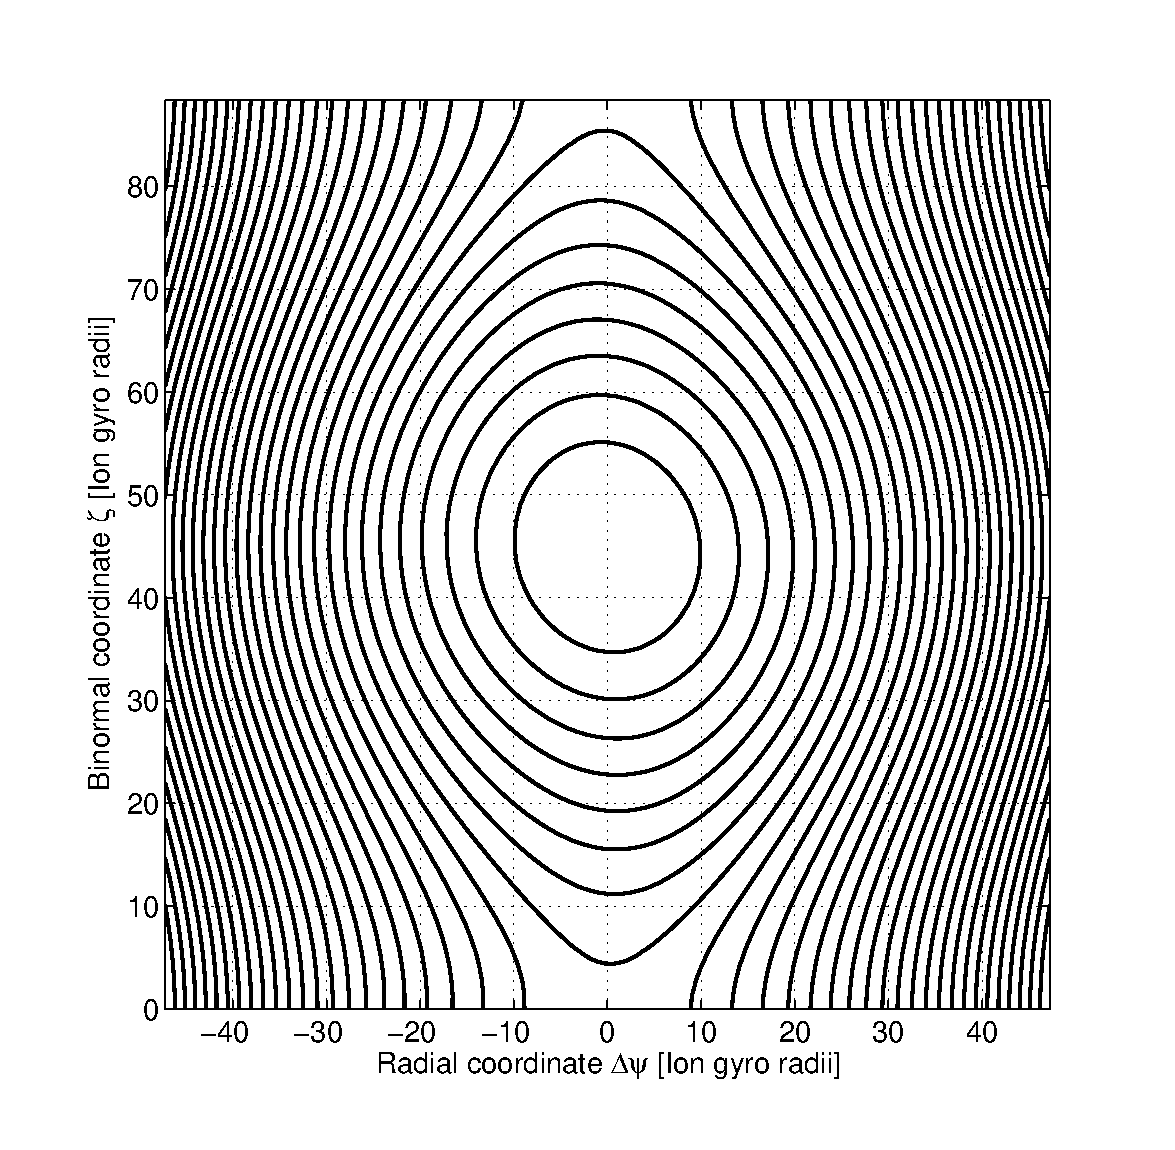
\includegraphics[width=0.3\textwidth]{MagIslGeom.eps}
\caption{Magnetic Island Geometry for an island with a half width of 30 ion gyro-radii}
\label{islandgeom}
\end{center}
\end{figure}

To run GKW with a magnetic island present the following options must be used:  Firstly, the code must be set to run electro-magnetically by setting \name{nlapar=.true.}.  In the \name{SPCGENERAL} namelist, \name{tearingmode} must be set to {\it .true.}, which adds the magnetic island as a perturbation of the equilibrium field.  The half width of the island is determined by the input parameter \name{wstar} which is the island width normalised to $\rho_{ref}$ (usually the ion gyro-radius).  A point of note is that this island width can not exceed (and should be smaller than) the radial extent of the computational box due to the periodicity constraints of a pseudo-spectral code. The rotation frequency of the island ($\omega$) is set by the parameter \name{isl\_rot\_freq}, normalised as other frequencies in the code BUT with opposite sign (positive is in the $\nabla \zeta$ direction, which is the electron grad-B drift direction when $s_j = 1$ and rln > 0.  By default the island is placed in the smallest non-zero poloidal wavevector (\name{isl\_mode=2}), however this can be changed by setting \name{isl\_mode} to another integer (e.g. \name{isl\_mode=3} will give 2 islands within the domain as the zero mode is always the first mode).

We recommend initialising the distribution function with \name{finit='zero'} as the island itself will seed the turbulence, and this gives faster convergence compared to non-zero distribution function initialisations.  When plotting XY profile outputs, setting {\it lisl_follow} in the \name{DIAGNOSTIC} namelist will follow the magnetic island so that the O-point is always in the centre of the box.  We do not recommend using the options to initialise the island after the turbulence, as growing the island too quickly drives a unphysical and large zonal flow, which initally supresses the turbulence and then takes a long time to decay.

\begin{small}
\begin{verbatim}
 &SPCGENERAL
 beta = 0.0001,  ! not used
 tearingmode=.true.,  wstar = 5.0,  finit = 'zero',  adiabatic_electrons = .false.
 Ls = 2.0,  isl_mode = 2, isl_rot_freq = 0.1   
 /
\end{verbatim}
\end{small}

\section{Spectral implementation of islands in 2D sheared slab geometry}

An alternative way to deal with 2D islands is also implemented, in which
parallel dynamics are projected into the $y$ direction, 
as is usually done in slab analytics.  This allows GKW islands to be compared
directly with analytical results in the slab.   Whilst this setup is intended for use with the slab geometry, 
it might also be applicable for a LFS toroidal case.
The island amplitude is decoupled from geometric magnetic shear, and 
a new parameter, \name{isl\_shear} is used in determing the island width.
To use this option the geometric shear \name{shat} is set to 0 (which
means reducing the coordinate system to purely Cartesian) and the code is
run with a single s point and without parallel dynamics 
(a limit in which the geometrical magnetic shear plays no role).
This also implies that the minimum $k_x$ and $k_y$ now can be set completely
independently, but they are chosen to be the same (to give a square box).

The perturbed $A_\parallel$ in this case then also contains the part of the island that
normally comes from the background magnetic field (in the 2D case the background B
plays no role in the geometry and theoretically only enters via the Larmor
radius). The slab geometry is defined in this case through a Cartesian set of
coordinates, $x$,$y$ and $z$, where $z$, the direction of the guide magnetic
field, is meant to be a symmetry coordinate for the whole system,
i.e. $\partial/\partial z = 0$, accordingly to the existing dedicated literature. 
The total magnetic field in this case reads
\begin{equation}
{\bf B} = B_z \nabla z -\nabla \psi \times \nabla z,
\end{equation}
with 
\begin{equation}
\psi = -\frac{i_s x^2}{2}B_z+\tilde{\psi}\cos( k_y y),
\label{psiisl}
\end{equation}
where $B_z$ is a constant and where  $i_s$ corresponds to \name{isl\_shear},
the (inverse of the) scale of variation of $B_y$, which plays a role analogous
to the magnetic shear in toroidal geometry. The $y$-dependent term represents
the island.  The amplitude $\tilde{\psi}$, assumed to be constant as a
consequence of the well-known ``constant-$\psi$ approximation'', is  linked to the island width $w$ through the relation
\begin{equation}
w^2=\frac{4 \tilde{\psi}}{i_s B_z}.
\end{equation}

In the 3D case, only the latter ``island''-part of $\psi$ is imposed as a
perturbation, entering the gyrokinetic equation through $v_\chi$ in the nonlinear term. 
In this 2D case, in constrast, we consider a shearless slab, with equilibrium 
\begin{equation}
{\bf B}= B_z \nabla z
\end{equation}
(constant) and we include the whole $\psi$ of Eq. \ref{psiisl}
as a perturbation. In Fourier space this extra island component
(additional to the usual part in the island $k_y$ mode)
is applied in the $k_y=0$ mode, and has the form 
\begin{equation}
A_\parallel^+(p) =  {4 (-1)^p i_s \over {\bar k}_x(p)^2 } \exp(-(p/Ls)^2)
\end{equation} 
where $p$ is again the radial mode number, and an exponential damping has again 
be added to the exact Fourier transformed quantity. The overbar on ${\bar k}_x$
represents the modes in the code, to distinguish them from the island wavenumbers $k_x$ and $k_y$
used above.  While it is apparent that $\psi$ is periodic on $y$, the
quadratic dependence on $x$ cannot be exactly reproduced in Fourier space, as
its derivative is not the same on the two boundaries. Thus, analogously to
the toroidal case, we again employ the exponential damping for the high $k_x$ modes in
order to remove boundary discontinuities.  This approximation has the effect of creating a second
magnetic island at the boundary which in full 3D geometry is obscured by parallel coupling, ballooning
and curvature. The effect of this boundary island can be minimised by 
choosing an appropriate combination of the parameters box size, shear, island width, damping length
(which differ in slab and torodial geometry) but it can never be completely eliminated.

In the 2D case, there is however an additional island option, to add \textit{two}
identical islands radially with perfect periodicity.  This option is activated
when \name{shat} = 0 and \name{isl\_shear} $> 0$ by selecting a
negative \name{wstar}. By choosing this option,  $\psi$ is
approximated by 
\begin{equation}
\psi = {\hat C}\cos{k_x x}+\tilde{\psi}\cos{k_y y},
\end{equation}
where $\hat{C}= \pi B_z i_s/ k_x^2$ is a constant chosen in order to have the
same amplitude as the other case for $B_y= \partial \psi/\partial$ at the edge
of the box. In this case, the additional nonzero component only appears in the $k_y=0$, $p= -1,1$ modes
with value $A_\parallel^+ = \pi i_s / k_x^2$.  The sinusoidal dependence can of course be implemented without any
approximation, or artificial damping, leading therefore to no parasitic boundary island
formation. However, the presence of both a maximum and a minimum in $x$
corresponds to the presence of two identical islands with $\pi/2$-shift in the
$y$-direction. By carefully choosing the box width, one is able to reduce the
mutual interaction of the two islands. 

Summarizing, for slab geometry GKW  has three options for islands:
\begin{itemize}
\item To run with shat $>$ 0 in 3D, which is expensive (and where
discontinuities at the boundary create numerical problems) and which does not
reproduce the boundary condition $\partial / \partial z =0$ used in many analytic models.
\item To run with shat = 0 and wstar $>$ 0. These are 2D runs, much faster, but which still
employ the artificial damping on high- ${\bar k}_x$ modes, and therefore require
specific attention to the discontinuity at the boundary, as in the full 3D cases.
\item To run with shat = 0 and wstar $<$  0. These are 2D runs, with no
artificial damping, but which contain two identical out of phase magnetic
islands at two radial locations.
\end{itemize}

Example 2D setup:
\begin{small}
\begin{verbatim}
 &GRIDSIZE
 NX = 167,  N_mu_grid = 8,  n_vpar_grid = 12, number_of_species = 2,
 N_s_grid = 1,  NMOD = 20,  nperiod = 1,
 /
 &MODE
 mode_box = .true., krhomax = 0.45, ikxspace = 1,
 /
 &GEOM
 GEOM_TYPE = 'slab_periodic', SHAT = 0.0,  Q = 1.0, EPS = 1.0,
 /
 &SPCGENERAL
 finit = 'zero',  tearingmode=.true.,
 wstar = 10.0, isl_rot_freq = -0.02,
 adiabatic_electrons = .false.
 ls=8.0, isl_shear = 0.1
\end{verbatim}
\end{small}

\section{Nonspectral implementation of a magnetic island}

If the radial direction is not treated in Fourier space, the implementation is much more direct, since we need only to introduce at $t=0$ the term
\begin{equation}
A_\parallel = A_{\parallel 0}\cos\left(2 \pi {\rm i} (m s - n \gamma )\right)
\end{equation}
which can be expressed by
\begin{equation}
A_\parallel = {1\over 2}A_{\parallel 0}\left[e^{i2\pi n\zeta}\left(\cos{\partial q \over \partial \psi} n s \Delta\psi - i\sin{\partial q \over \partial \psi} n s \Delta\psi\right)
+ e^{-i2\pi n\zeta}\left(\cos{\partial q \over \partial \psi} n s \Delta\psi + i\sin{\partial q \over \partial \psi} n s \Delta\psi\right)\right]
\end{equation}

In the binormal direction we initialise only one mode, namely $e^{i2\pi n\zeta}$ and assume the existence of the other mode in other to get a real quantity once the inverse Fourier transform is performed. Therefore,
 we need to implement only the potential
 \begin{equation}
A_{\parallel,+} = {1\over 2}A_{\parallel 0}\left(\cos{\partial q \over \partial \psi} n s \Delta\psi - i\sin{\partial q \over \partial \psi} n s \Delta\psi\right)
\end{equation}

In order to decouple the island from the boundary of the simulation box, we multiply the previous potential by a radial envelope having the explicit expression
\begin{equation}
A_r\left(\Delta\psi\right) = {1\over 4}\left(1+\tanh\left({\Delta\psi+\Delta\psi_0\over \delta\psi_0}\right)\right)\left(1-\tanh\left({\Delta\psi-\Delta\psi_0\over \delta\psi_0}\right)\right)
\end{equation}
where $\Delta\psi_0$ and $\delta\psi_0$ are defined in the tearingmode namelist of the input file of GKW by the variables \File{psi_0} and \File{delta_psi_0}, respectively.

In a 2D sheared slab geometry, the previous implementation reduces to
\begin{equation}
A_\parallel = {1\over 2}A_{\parallel 0}A_r\left(\Delta\psi\right)
\end{equation}
and the background magnetic shear is introduced together with this perturbation by means of the mode $\kappa_\zeta=0$. Therefore, the total parallel vector potential reads in 2D sheared slab geometry
\begin{equation}
A_\parallel = {B_zi_s\over 2}\left[\Delta\psi^2-\left(L_x/2\right)^2\right]+{1\over 2}A_{\parallel 0}A_r\left(\Delta\psi\right)e^{i2\pi n\zeta}
\end{equation}
where the additional term ${B_zi_s\over 2}\left(L_x/2\right)^2$ is introduced to impose a vanishing potential at the boundary in the nonspectral version. We therefore need to introduce the term ${B_zi_s\over 2}\left[\Delta\psi^2-\left(L_x/2\right)^2\right]$ in the $\kappa_\zeta=0$ component and the term ${1\over 2}A_{\parallel 0}A_r\left(\Delta\psi\right)$ in the $\kappa_\zeta = \kappa_{\rm isl}$ component.

\section{Reconstruction of flux tube radial profiles \label{profiles} and profile flattening in GKW}

The benchmark of the magnetic islands implementation includes the flattening of the density and pressure profiles. The equilbrium profiles are linear with respect to the radial coordinate and are present in the source terms.  Since we are solving the gyrokinetic equation for the perturbed part of the distribution function, the solution should respond to the source terms due to the background. In particular, the magnetic island should give a perturbation that cancels the background out inside the separatrix. Note that runs must be non-linear for the correct level of flattening to be obtained. To reconstruct the radial profiles the XY diagnostics must enabled in the diagnostics namelist.

% \begin{verbatim}
% &DIAGNOSTIC
%  lisl_follow = .false.,
%  lphi_diagnostics = .true.,
%  xy_phi = .true.,
%  xy_apar = .true.,
%  xy_fluxes = .true.,
%  xy_fluxes_em = .true.,
%  xy_dens = .true.
%  xy_current = .true.,
%  xy_temp = .true.,
%  / 
% \end{verbatim}

\subsection{Density profiles}

The files named \File{den0\#_000*_*} hold the normalised XY perturbed density data ($\tilde{n}_{N,s}$) for each large time step. The background density profile can be reconstructed by using the local radial cordinate $x_r = \psi / \rho_* = r / \rho_{\rm ref}$ which is written in the file named \name{xphi} (with the same dimensions as the XY slices) and the input parameter \name{RLN_s} = $-(1/n_{R_0,s}) {\partial n_{R_0,s} \over \partial \psi}$. The total density of species $s$ is $n_s = n_{s,\rm eq} + \tilde{n}_s$, where $n_{s,\rm eq} = n_{R_0,s}\left(1-{r-r_0\over L_{n,s}}\right)$ is the global density of the Maxwellian equilibrium written in the local limit, i.e. $n_{R_0,s}$ at the resonant position $r_0$ plus the linear variation due to the gradient at that position. Note that in the expression of $n_{s,\rm eq}$, the quantity $n_{R_0,s}$ does not exhibit any radial dependence since it is considered in the local limit. The perturbed density of species $s$ is

\begin{equation}
\tilde{n}_s = \int_{\mathbb R^3} d^3\mathbf{v}\delta f_s = \rho_*n_{R_0,s}\int_{\mathbb R^3} d^3\mathbf{v}_{N,s}\delta f_{N,s} = \rho_*n_{R_0,s}\tilde{n}_{N,s}
\end{equation}

Therefore, the total density for species $s$ reads

\begin{equation}
n_s = n_{R_0,s}\left(1-{r-r_0\over L_{n,s}}\right) + \rho_*n_{R_0,s}\tilde{n}_{N,s} = n_{R_0,s}\left(1 - {\left(x_r-x_{r0}\right)\rho_{\rm ref}\over {L_{n,s}}}\right) + \rho_*n_{R_0,s}\tilde{n}_{N,s}
\end{equation}

We can now normalise the density for species $s$ as $n_{N,s} = n_s / n_{R_0,s}$

\begin{equation}
n_{N,s} = \left(1 - {\left(x_r-x_{r0}\right)\rho_{\rm ref}\over {L_{n,s}}}\right) + \rho_*\tilde{n}_{N,s}
\end{equation}
and define the change in the density for species $s$ as $\Delta n_{N,s} = n_{N,s} - 1$

\begin{equation}
 \Delta n_{N,s} = - \left(x_r-x_{r0}\right){\rho_{\rm ref}R_{\rm ref}\over {L_{n,s}R_{\rm ref}}} + \rho_*\tilde{n}_{N,s}  =  - \rho_* \left(x_r-x_{r0}\right) {R_{\rm ref}\over L_{n,s}} + \rho_*\tilde{n}_{N,s}
\end{equation}
or alternatively
\begin{equation}
{\Delta n_{N,s} \over \rho_*} = \tilde{n}_{N,s} - {R_{\rm ref} \over L_{n,s}} \left(x_r-x_{r0}\right)
\end{equation}
and the total density gradient (background plus perturbed density) can be computed as
\begin{equation}
{R_{\rm ref} \over L_{n_{\rm eq}+\tilde{n}}}  =  -{1 \over n_{R_0,s}} {\partial (n_{s,\rm eq}+\tilde{n}_s) \over \partial \psi} = 
 -{\partial \tilde{n}_{N,s} \over \partial x_r} + {R_{\rm ref} \over L_{n,s}}.
\end{equation}

%PREVIOUS VERSION needs a factor rho_* to get to a normalised total density (i.e. it has the normalisation of delta f, not F_M)
%\begin{equation}
%n({\Delta\psi}) = \tilde{n} - RLn*xphi
%\end{equation}

\subsection{Pressure profiles}
To obtain the pressure profiles we need to use the files \File{ene0\#_000*_*}, which hold the normalised second moments of the distribution function, namely
\begin{equation}
\tilde E_{N,s} = \int_{\mathbb{R}^3}d^3\mathbf{v}_{N,s}\delta f_{N,s}v_{N,s}^2
\end{equation}

It can be shown that the pressure perturbation is written in terms of this quantity as follows
\begin{equation}
\tilde{p}_s = {1\over 3}m_{\rm ref}v_{th,s}^2\rho_* n_{R_0,s}m_{R,s}\tilde E_{N,s}
\end{equation}

Taking into account the definition of the reference temperature $T_{\rm ref}$, one can write

\begin{equation}
\tilde{p}_s = {2\over 3}\rho_* n_{R_0,s}T_{\rm ref}m_{R,s}v_{R,s}^2\tilde E_{N,s}
\end{equation}

In addition, $m_{R,s}v_{R,s}^2=T_{R,s}$ and $T_s = T_{\rm ref}T_{R,s}$, which leads to
\begin{equation}
\tilde{p}_s = {2\over 3}\rho_* n_{R_0,s}T_s\tilde E_{N,s}
\end{equation}

In the same way as has been done with the density, the total pressure is defined as $p_s = p_{s,\rm eq} + \tilde{p}_s$, where $p_{s,\rm eq} = n_{R_0,s}T_s\left(1-{r-r_0\over L_{n,s}}\right)\left(1-{r-r_0\over L_{T,s}}\right)$. In the local limit we can neglect terms of second order in $\rho_*$ and therefore, the equilibrium pressure profile reads
\begin{equation}
p_{s,\rm eq} \approx n_{R_0,s}T_s\left(1-\rho_*\left(x_r-x_{r0}\right){R_{\rm ref}\over L_{n,s}}-\rho_*\left(x_r-x_{r0}\right){R_{\rm ref}\over L_{T,s}}\right)
\end{equation}

We can now divide by $n_{R_0,s}T_s$ and define the change in the normalized pressure as

\begin{equation}
\Delta p_{N,s} = {2\over 3}\rho_*\tilde E_{N,s}-\rho_*\left(x_r-x_{r0}\right){R_{\rm ref}\over L_{n,s}}-\rho_*\left(x_r-x_{r0}\right){R_{\rm ref}\over L_{T,s}}
\end{equation}
or equivalently
\begin{equation}
{\Delta p_{N,s} \over \rho_*} = {2\over 3}\tilde E_{N,s}-\left(x_r-x_{r0}\right){R_{\rm ref}\over L_{n,s}}-\left(x_r-x_{r0}\right){R_{\rm ref}\over L_{T,s}}
\end{equation}

This quantity is plotted in figure \ref{fig:pressureflat}. Note that the flattening is observed in the moments of the distribution function, namely the density and the pressure. One can define a temperature for the unperturbed profiles, since these unperturbed quantities are obtained from a Maxwellian equilibrium. However, one cannot say that the total pressure is $p=nT$, where $n=n_{\rm eq} + \tilde{n}$ and $T_{\rm eq} + \tilde{T}$. For this reason, the flattening of the profiles can only be analysed for the density and the pressure. An example of unexpected results that one can obtain when defining a perturbed temperature is evidenced when introducing a magnetic island in a plasma with flat temperature profile but finite density gradient. One expects that the temperature is not modified, since it is already flat. However, by defining the temperature as $T=p/n$ one obtains a modification which actually corresponds to the modifications of both density and pressure.

\begin{figure}
\begin{center}
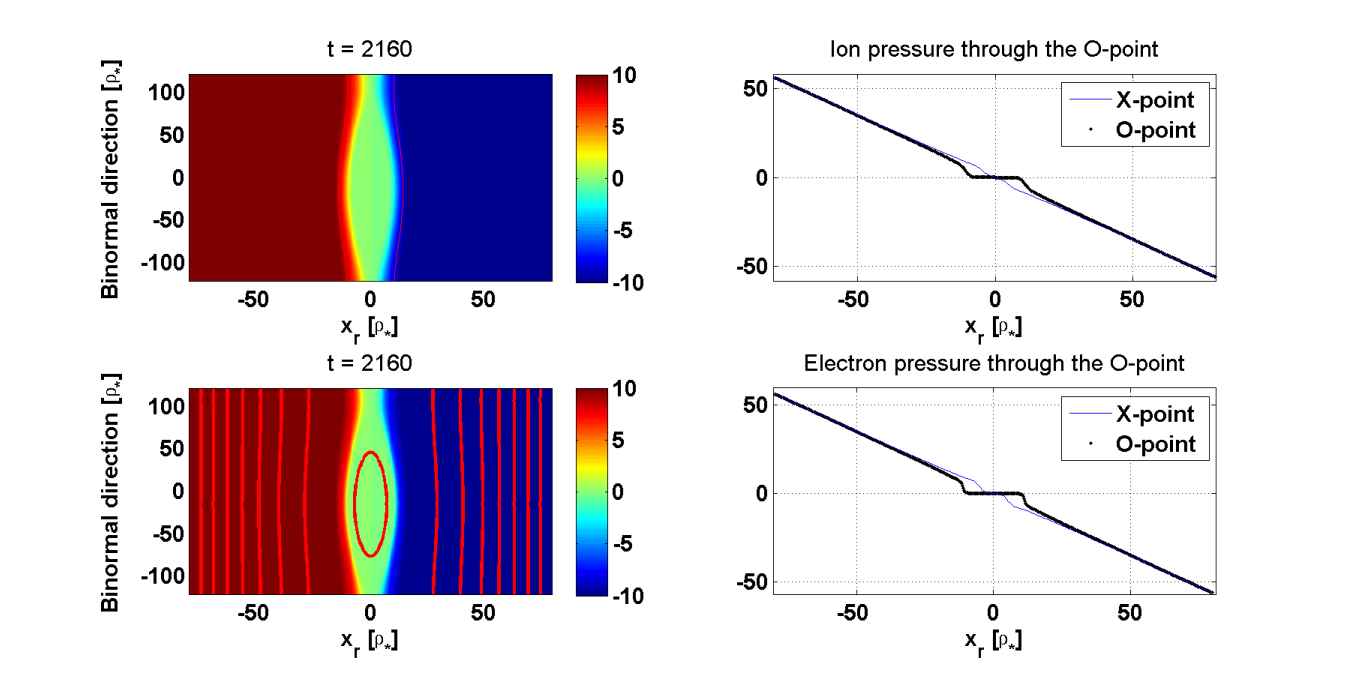
\includegraphics[width=0.7\textwidth]{pressflat.eps}
\caption{Left: 2D colormap of the pressure profiles for ions and electrons in the presence of a magnetic island. The isocontours of the vector potential are shown only with the electron colormap. Right: radial profiles of the pressure through the O (black line) and X (blue line) points.}
\label{fig:pressureflat}
\end{center}
\end{figure}

The total pressure gradient (background plus perturbed pressure) reads
\begin{equation}
{R_{\rm ref} \over L_{p_{\rm eq}+\tilde{p}}}  =  -{1 \over n_{R_0,s}T_s} {\partial (p_{s,\rm eq}+\tilde{p}_s) \over \partial \psi} = -{\partial\over\partial x_r}{\Delta p_{N,s} \over \rho_*} = 
 -{2\over 3}{\partial\tilde E_{N,s}\over\partial x_r} + {R_{\rm ref} \over L_{n,s}} + {R_{\rm ref} \over L_{T,s}}
\end{equation}

\section{Frozen electrons}

Due to the small inertia of electrons, they are considered as frozen particles to the magnetic field lines. This means in particular that the rotation frequency of electrons must equal the rotation
frequency of the island, namely
\begin{equation}
\omega_{\rm isl}\equiv\omega_{\rm TOT,e} = \omega_{*,e} + \omega_{E\times B}
\end{equation}
which constitutes the second benchmark after implementation of a magnetic island.

Therefore, the electric field must always compensate for the difference between the diamagnetic drift produced by any pressure gradient inside the island and the rotation of the island itself. In particular,
if the island does not rotate, for a sufficiently large island resulting in a complete flattening, the electrostatic potential must vanish inside the island. To verify the previous identity, one must
 conveniently quantify from the GKW outputs the diamagnetic frequency resulting from the total pressure profile and the $E\times B$ frequency.
These two quantities are derived hereafter assuming a slab geometry and considering that the binormal (in the $y$ direction) structure is determined by the island. The diamagnetic frequency in the $y$ direction reads
\begin{equation}
\omega_{*,s} = k_y{{\mathbf{b}\times\nabla p_s}\over{e_sn_sB}}\cdot\mathbf{e}_y\approx k_y{1\over{e_sn_{s,\rm eq}B}}{\partial p_s\over{\partial r}}
\end{equation}

Using the normalizations of GKW, we can write
\begin{equation}
\omega_{*,s} \approx k_y{1\over{e_{N,s}en_{R_0,s}B_NB_{\rm ref}}}{{n_{R_0,s}T_s\rho_*}\over{\rho_{\rm ref}}}{\partial\over{\partial x_r}}{\Delta p_{N,s} \over \rho_*}
\end{equation}

The temperature $T_s$ can now be expressed in terms of $T_{\rm ref}$ and $T_{R,s}$ and the reference Larmor radius used to write
\begin{equation}
\omega_{*,s} \approx k_y{1\over 2}v_{\rm th,ref}{T_{R,s}\over e_{N,s}B_N}\rho_*\left({2\over 3}{\partial\tilde E_{N,s}\over\partial x_r} - {R_{\rm ref} \over L_{n,s}} - {R_{\rm ref} \over L_{T,s}}\right)
\end{equation}

Under the assumption that the $y$ structure is determined by the island, one can write the wave number is that direction as $k_y=\pi/y_{\rm max}$, where $y_{\rm max}$ is the maximum value of the $y$ coordinate. Expressing $\rho_*$ as $\rho_*=\rho_{\rm ref}/R_{\rm ref}$ and normalizing the diamagnetic frequency to the transit frequency $\omega_t = v_{\rm th,ref}/R_{\rm ref}$ one gets the normalized diamagnetic frequency in slab geometry
\begin{equation}
\omega_{*,N,s} \approx {\pi\over y_{\rm max,N}}{1\over 2}{T_{R,s}\over e_{N,s}B_N}\left({2\over 3}{\partial\tilde E_{N,s}\over\partial x_r} - {R_{\rm ref} \over L_{n,s}} - {R_{\rm ref} \over L_{T,s}}\right)
\end{equation}

In a similar way, one can show that the $E\times B$ frequency in GKW units reads
\begin{equation}
\omega_{E,N,s} \approx {\pi\over y_{\rm max,N}}{1\over 2}{1\over B_N}{\partial\phi_{N}\over\partial x_r}
\end{equation}

Figure \ref{fig:freqsmatching} represents the profiles of the frequency for each species in the presence of an island rotating in the ion diamagnetic direction with a frequency $\omega_{\rm isl} = -0.006$. This frequency is represented by a solid black line, which must overlap the solid green line, corresponding to the total frequency of electrons. We observe this overlap everywhere inside the separatrix, but not around the X-point.

\begin{figure}
\begin{center}
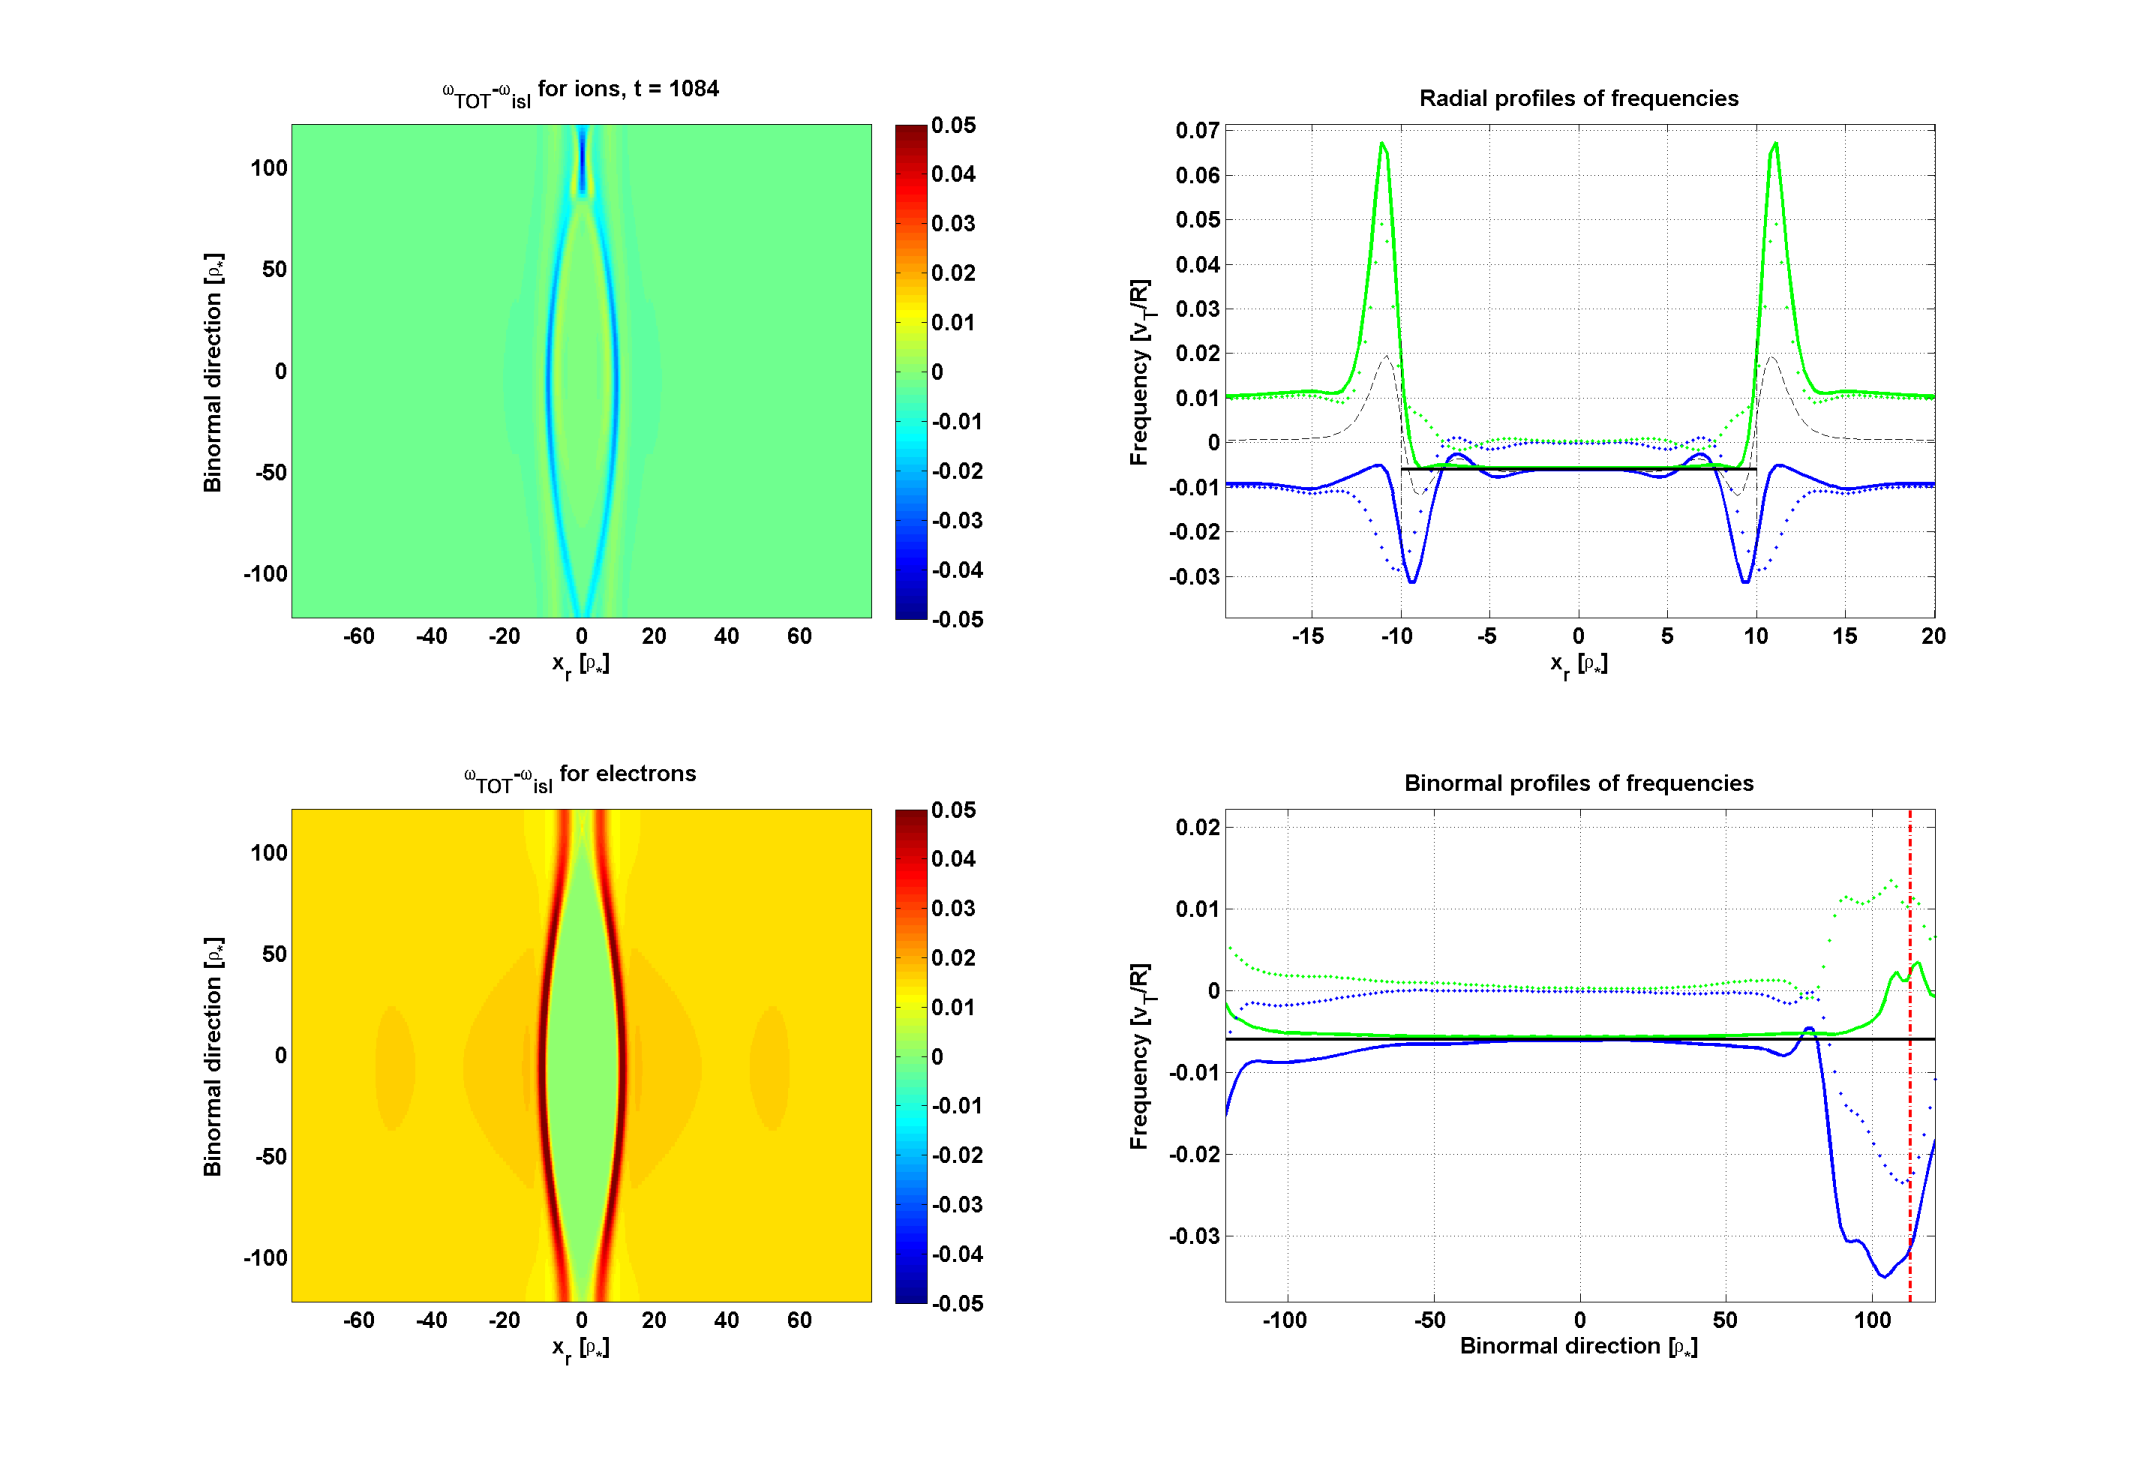
\includegraphics[width=0.7\textwidth]{freqsmatching.eps}
\caption{Left: 2D colormap of the frequency profiles for ions (up) and electrons (down) in the presence of a magnetic island with $R/L_n=0.7$ and $R/L_T=0$. Right: radial profiles of the frequency through the O-point (up) and binormal profiles of the frequency through the O and X points (down). Electrons are represented by green curves and ions by blue curves. The dotted lines represent the diamagnetic frequency and the solid lines the total frequency. For the radial profiles, the black dashed line represents the $E\times B$ frequency and the solid black line the rotation frequency of the island. For the binormal profiles, the dashed red line indicates the position of the X-point and the solid black line the rotation frequency of the island.}
\label{fig:freqsmatching}
\end{center}
\end{figure}

\section{Dependence of the electrostatic potential on the island rotation frequency}

The third and last benchmark needed after the implementation of a magnetic island constitutes the dependence of the electrostatic potential on the island rotation frequency. This dependence is calculated assuming that
 electrons inside the island short out any variation of the parallel electric field, i.e. we need to verify that $\nabla_\parallel\phi=-c^{-1}\partial_t \psi$ inside the island.
  For this we need to write an explicit expression for the parallel gradient, which is $\nabla_\parallel = \mathbf{b}\cdot\nabla$, where $\mathbf{b}=B^{-1}\mathbf{B}$ is the unit vector in the direction of the magnetic field.
  Let us perform the calculation, for the sake of simplicity, in sheared 2D slab geometry, where the magnetic field reads
  \begin{equation}
  \mathbf{B} = B_z\nabla z - \nabla\psi\times\nabla z = B_z\nabla z + {B_z x \over L_s}\nabla y - \tilde\psi k_y\sin\left(k_yy-\omega_{\rm isl}t\right)\nabla x
  \end{equation}

Under the assumption that the amplitude of the magnetic field is not significantly modified by the presence of the magnetic island and considering no derivatives in the $z$-direction (slab model), we can write
\begin{equation}
\nabla_\parallel = - {\tilde\psi k_y\over B_z}\sin\left(k_yy-\omega_{\rm isl}t\right)\partial_x + {x \over L_s}\partial_y
\end{equation}

The equation for the electrostatic potential is written as
\begin{equation}
{\tilde\psi k_y\over B_z}\sin\left(k_yy-\omega_{\rm isl}t\right){\partial\phi\over\partial x} - {x \over L_s}{\partial\phi\over\partial y} = {1\over c}{\partial \psi\over\partial t}
\end{equation}

Noticing that $x$ and $y$ coordinates must be related to each other on a flux surface for a given time $t$ by the flux label
\begin{equation}
\Omega = {x^2B_z \over 2\tilde\psi L_s} - \cos\left(k_yy-\omega_{\rm isl}t\right)
\end{equation}
we can rewrite the equation satisfied by the electrostatic potential as follows
\begin{equation}
- {x \over L_s}{\partial\phi\over\partial y} = {1\over c}{\partial \psi\over\partial t},\,\,\,\,\,{\rm for}\,\,d\Omega=0
\end{equation}
or equivalently
\begin{equation}
- {x \over L_s}\left.{\partial\phi\over\partial y}\right\vert_{\Omega} = {1\over c}{\partial \psi\over\partial t}
\end{equation}
The derivative of $x$ with respect to $y$, for $x\ne 0$, reads
\begin{equation}
{dx\over dy} = -{\tilde\psi L_s\over B_z x}\sin\left(k_yy-\omega_{\rm isl}t\right)
\end{equation}
and therefore, the equation satisfied by the electrostatic potential becomes, for $k_yy\not\equiv_\pi\omega_{\rm isl}t$
\begin{equation}
{k_y\over B_z}\left.{\partial\phi\over\partial x}\right\vert_{\Omega} = {\omega_{\rm isl}\over c}
\end{equation}
which gives, after integration
\begin{equation}
\phi = {\omega_{\rm isl}B_z\over k_y c}\left(x-h\left(\Omega\right)\right)
\end{equation}
where $h\left(\Omega\right)$ is a constant of integration for each flux surface. Note that the expression we have obtained for the electrostatic potential is only valid for $x\ne 0$ and $k_yy\not\equiv_\pi\omega_{\rm isl}t$. The function $h\left(\Omega\right)$ usually vanishes inside the island, corresponding to a complete flattening of radial profiles. Therefore, inside the separatrix and for $x\ne 0$ we can write, in GKW units
\begin{equation}
\phi_N = 2{\omega_{\rm isl,N}y_{\rm max,N}\over \pi}\Delta x_r
\end{equation}
where $\Delta x_r$ is the distance to the resonant surface. The extension to $x=0$ and $k_yy\equiv_\pi\omega_{\rm isl}t$ can be done by assuming that the electrostatic potential is continuous. Therefore, $\phi(x=0)=\lim_{x\rightarrow 0^\pm}\phi = 0$, $\phi(x=w,k_yy\equiv_\pi\omega_{\rm isl}t)=\lim_{x\rightarrow w^+}\phi = 2{\omega_{\rm isl,N}y_{\rm max,N}\over \pi}w$ and $\phi(x=-w,k_yy\equiv_\pi\omega_{\rm isl}t)=\lim_{x\rightarrow -w^-}\phi = -2{\omega_{\rm isl,N}y_{\rm max,N}\over \pi}w$. The left panel of figure \ref{fig:phiseparatrix} shows a remarkable agreement between the expected values for the electrostatic potential at the separatrix ($\Delta x_r = w$)
 from the previous expression (solid black line) and the values obtained from five simulations with GKW (red asterisks). These simulations have been performed with $w=10$, $y_{\rm max,N}=121.565$ and flat profiles.
\begin{figure}
\begin{center}
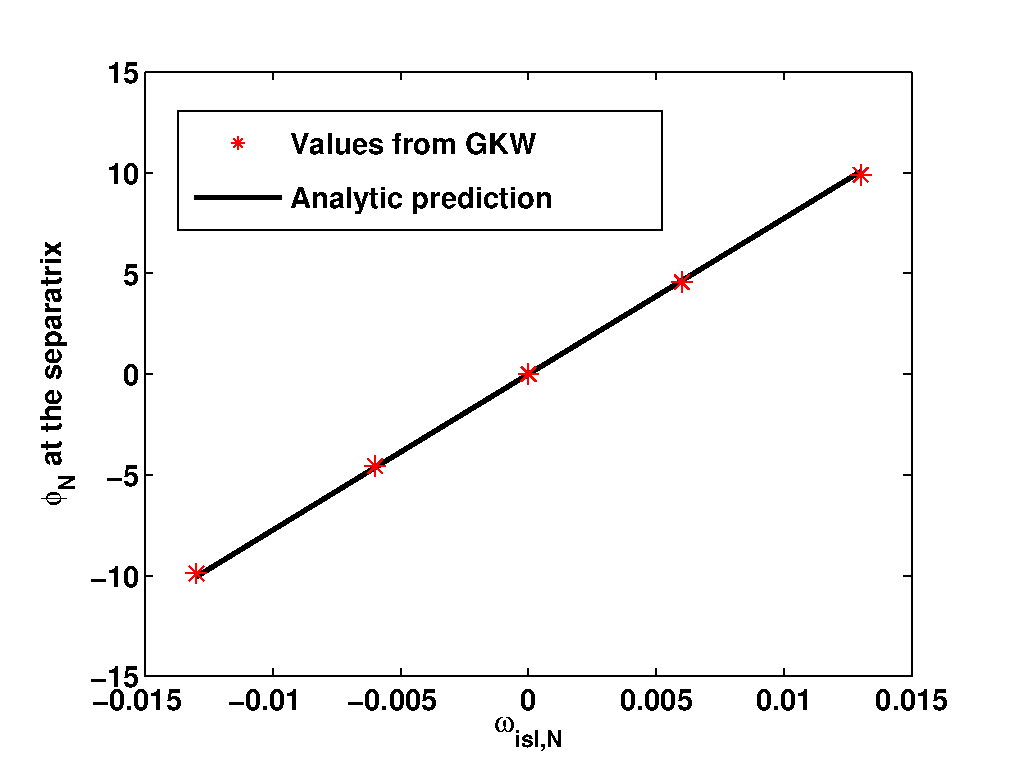
\includegraphics[width=0.4\textwidth]{phiseparatrix.eps}
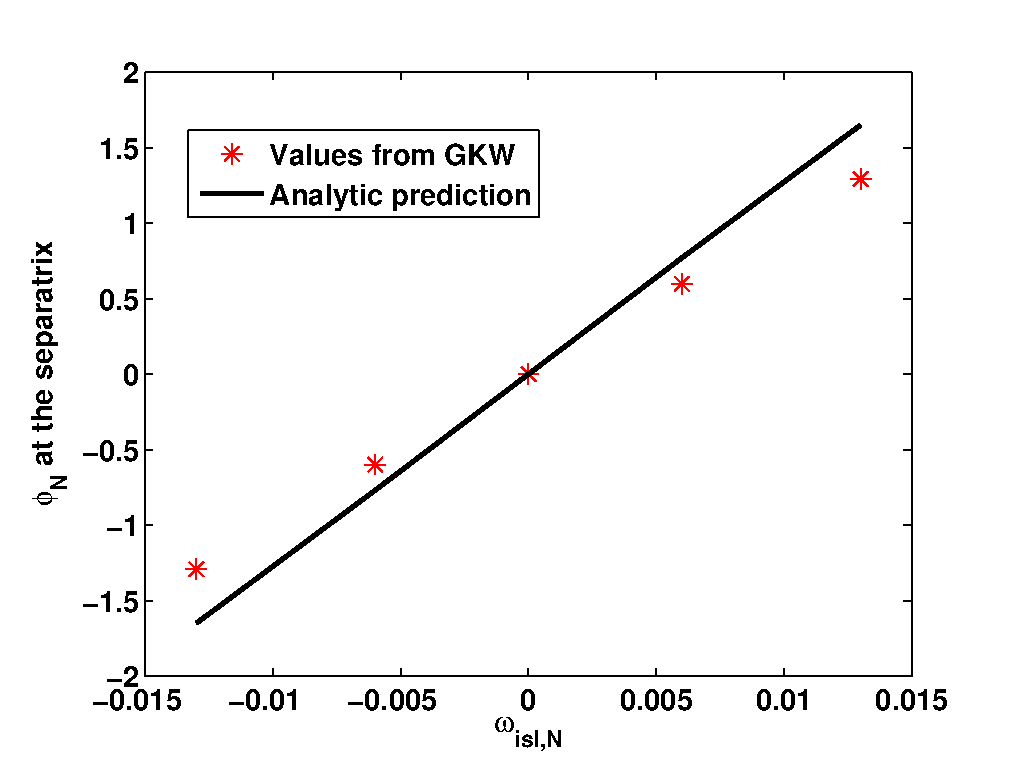
\includegraphics[width=0.4\textwidth]{phiseparatrixw2.eps}
\label{fig:phiseparatrix}
\caption{Expected values of the electrostatic potential at the separatrix (solid black line) and values obtained from simulations with GKW (red asterisks). Left: $w=10$. Right: $w=2$}
\end{center}
\end{figure}

When the island width is comparable to or smaller than the ion Larmor radius, the ion pressure profile is little modified, whereas the electron pressure profile inside the island can still be modified.
 Of course, in the absence of background density and temperature profiles, this means that the ion pressure remains almost flat, whereas the electron pressure is only modified around the separatrix. However, this
  modification is of the order of the ion Larmor radius, meaning that for an island width of the order of the ion Larmor radius the electron pressure profile will be modified inside the island.
   In this case, the equation satisfied by the electrostatic potential should include the term related to the parallel gradient of the electrons pressure inside the island, namely
\begin{equation}
\nabla_\parallel\phi=-c^{-1}\partial_t \psi + {1\over en_e}\nabla_\parallel p_e
\end{equation}

Integrating this equation leads straightforwardly to the expression
\begin{equation}
\phi = {\omega_{\rm isl}B_z\over k_y c}\left(x-h\left(\Omega\right)\right) + {1\over en_e}p_e
\end{equation}
or equivalently, in GKW units
\begin{equation}
\phi_{N,\rm sep} = 2{\omega_{\rm isl,N}y_{\rm max,N}\over \pi}w + \left.{\Delta p_{N,s} \over \rho_*}\right\vert_{\rm sep}
\end{equation}

The right panel of figure \ref{fig:phiseparatrix} shows quite a good agreement, but some differences are observed. More analysis is needed for a complete understanding in the case of small islands.


% related to auctex mode and latex-preview-mode in Emacs:
%%% Local Variables:
%%% mode: latex
%%% TeX-master: "doc"
%%% End:

\chapter{Eigenvalue solver}
\label{ch:eiv}

Here we give some information on the usage of the eigenvalue solver, implemented
in GKW, as well as some technical details. 
Further information can be found in the presentation of R. Buchholz on the GKW webpages under Talks.

As the system size of the linear gyrokinetic equation is too big for a direct numerical solution, projection
methods are used.
For a brief introduction to projection methods, see the {\sc slepc} manual \cite{SLE12} and references therein.


\section{Usage}
\label{sec:eivusage}
First, GKW must be compiled with {\sc slepc/petsc}, see \ref{subsubsec:slepc}
for details.

The easiest way to create an input file for the eigenvalue solver is the following:
First, set up an input file which uses explicit time
integration.
As second step then replace \name{METHOD = 'EXP'} with \name{METHOD='EIV'}
and  set \name{METH=1}. It is recommended to set a low value \name{NAVERAGE} like \name{NAVERAGE=1}.
Setting \name{METH=2} or \name{NAVERAGE$\gg$1} works too, but the run is then usually slower.

The third and final step is to set the parameters for the eigenvalue solver
itself. This is done in the namelist \name{eiv_integration},
an example of which is given below.
One has to select the portion of the spectrum to be sought with the parameter \name{which_eigenvalues}. Available options are listed in the sample input file.
In addition, you can choose between two methods for extracting eigenvalues,
\name{type_extraction = 'harmonic'}, and \name{type_extraction = 'ritz'}.
Note that with \name{type_extraction = 'harmonic'} the target values \name{growthrate} and \name{freq}) are always used. 

Unfortunately it is difficult to recommend optimal settings in advance,
or even settings which will guarantee to find physically interesting eigenmodes of the system.

One rule seems to be valid in general:
If you use harmonic extraction and search for the mode with largest
eigenvalue, you should keep the target frequency \name{freq=0.0}.  
If you don't find an eigenvalue, increase the target \name{growthrate}, 
while if you just find stable high frequency eigenmodes, decrease it.

To share some experiences, fig. \ref{fig:eivharmonicgrowth}--\ref{fig:eivtargetsa} 
show scans for two sets of parameters.
\begin{figure}[htp!]
  \begin{center}
    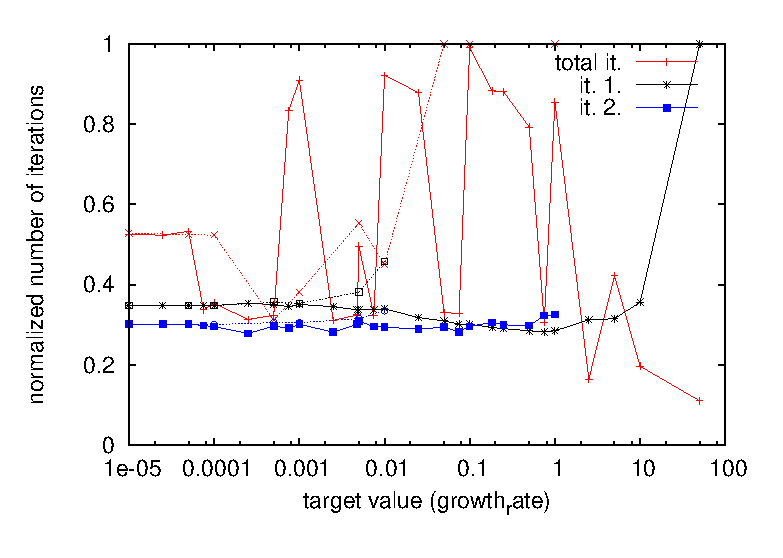
\includegraphics[width=0.8\textwidth]{HarmonicGrowth}
    \caption{\label{fig:eivharmonicgrowth} Scan over growth rate with
    frequency set to zero. Dashed lines depict negative values of
    \name{growthrate}. Normalization is done with the maximum number of
    iterations for the first/second eigenvalue/total number of iterations,
    respectively.}
  \end{center}
\end{figure}
\begin{figure}[htp!]
  \begin{center}
    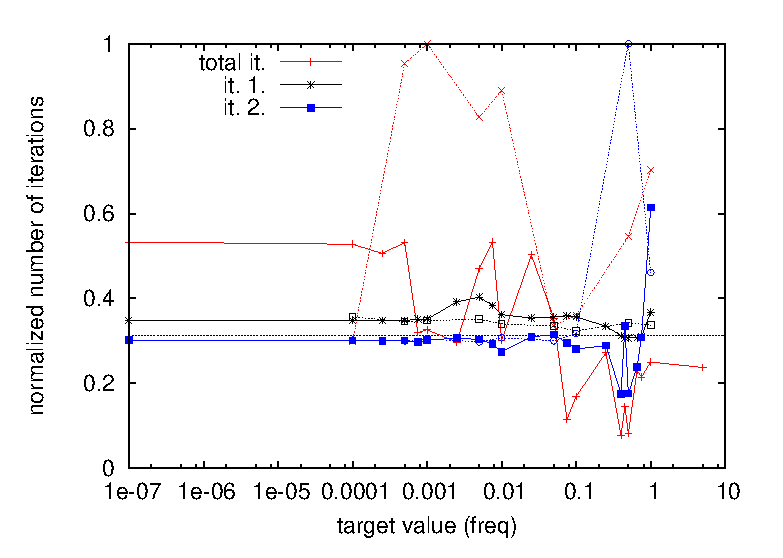
\includegraphics[width=0.8\textwidth]{HarmonicFreq}
    \caption{\label{fig:eivharmonicfreq} Scan over frequency with growth rate
      set to zero. Dashed lines depict negative values of \name{freq}. The
      point at $10^{-7}$ actually had zero frequency. Normalization is as for
      fig. \ref{fig:eivharmonicgrowth}. The dashed-dotted line depicts the
      minimum value for the total iterations of fig. \ref{fig:eivharmonicgrowth}
      (only counting points where both unstable eigenmodes are found).}
  \end{center}
\end{figure}
\begin{figure}[htp!]
  \begin{center}
    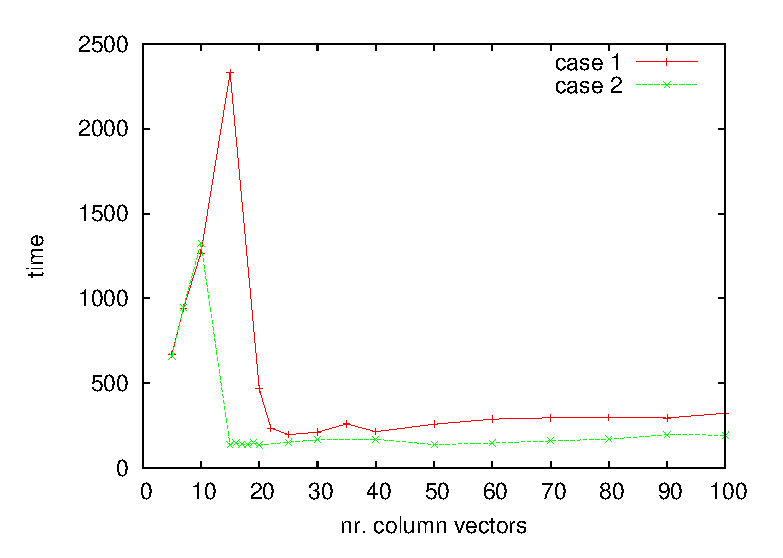
\includegraphics[width=0.8\textwidth]{HarmonicNcv}
    \caption{\label{fig:eivharmonicncv} Scan over size of subspace  (\name{nr\_column\_vec}), for one
    point of each of the other two scans. First case: \name{growthrate = 0.0},
    freq = 0.45, searching for 5 eigenpairs (default value: 20). Second case: growthrate = 2.50E-3,
    freq = 0.0, searching for 2 eigenpairs (default value: 17).}
  \end{center}
\end{figure}

The input parameters for fig. \ref{fig:eivtargets1}--\ref{fig:eivtargetsa} are
based on the \File{STD_linear_ITG} and \File{simple_TEM} input files found in
\File{doc/input}, with $R/L_{T_i} = 6$, which is near the ITG-TEM transition.
Two unstable eigenmodes are therefore expected.
Scans were made over the target \name{growthrate} and \name{freq} for the harmonic extraction.
The fixed parameters for the eigenvalue solver were
\begin{verbatim}
max_iterations = 30000
tolerance = 1.0e-6
type_solver = 'krylovschur'
type_extraction = 'harmonic'
number_eigenvalues = 3 ! just in case there are more unstable ones than expected
nr_column_vec      = 20
mat_vec_routine    = 1
which_eigenvalues =  1 ! largest magnitude
\end{verbatim}

\begin{figure}[htp!]
  \begin{center}
    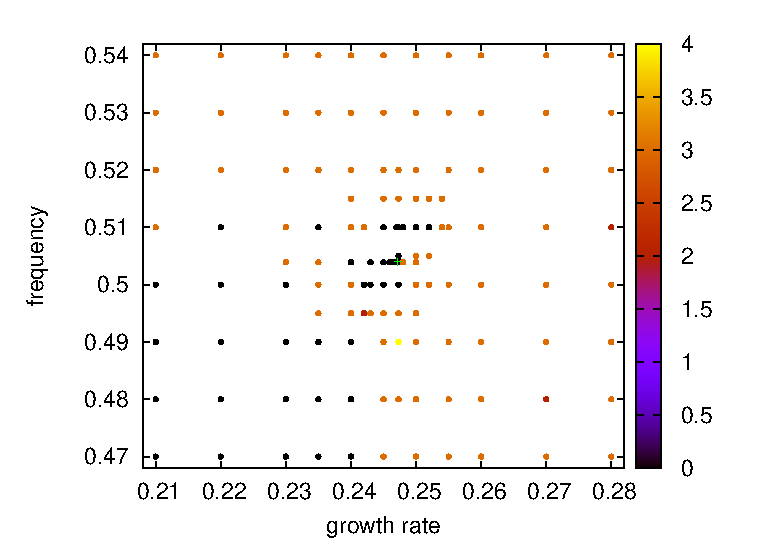
\includegraphics[width=0.8\textwidth]{Targets}
    \caption{\label{fig:eivtargets1} A scan over target values near the ITG,
      searching for eigenvalues with largest magnitude.
      Plus signs refer to actual found eigenvalues, crosses to 'conjugated'
      eigenvalues, stars to the projections on the growth rate axis. Color
      of the dots refers to the number of found eigenvalues. Please note, that
      a value of 1(or more) requires that the fastest growing eigenmode was found and
      a value of 2(or more) requires that both fastest growing eigenmodes where found.
      Harmonic extraction was used.      
}
  \end{center}
\end{figure}
\begin{figure}[htp!]
  \begin{center}
    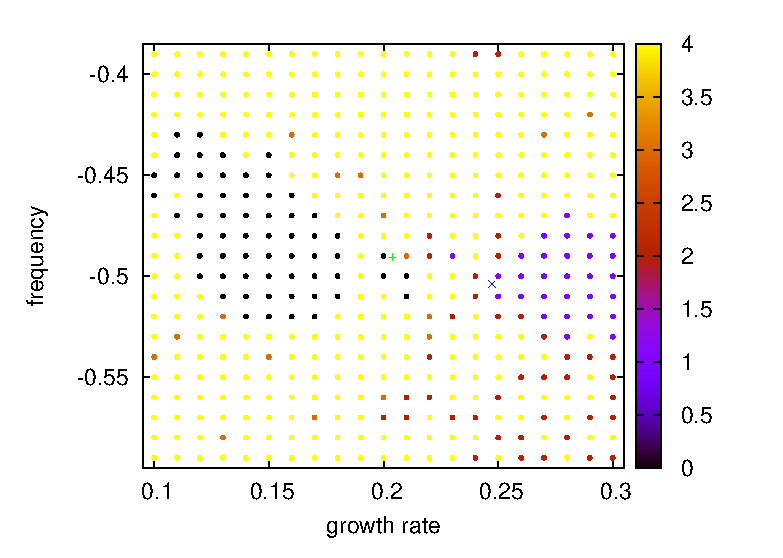
\includegraphics[width=0.8\textwidth]{Targets2}
    \caption{\label{fig:eivtargets2} A scan analogous to \ref{fig:eivtargets1}, 
      but target values are near the TEM eigenvalue.
      For the meaning of the symbols please refer to the caption of fig.
      \ref{fig:eivtargets1}.}
  \end{center}
\end{figure}
\begin{figure}
  \begin{center}[htp!]
    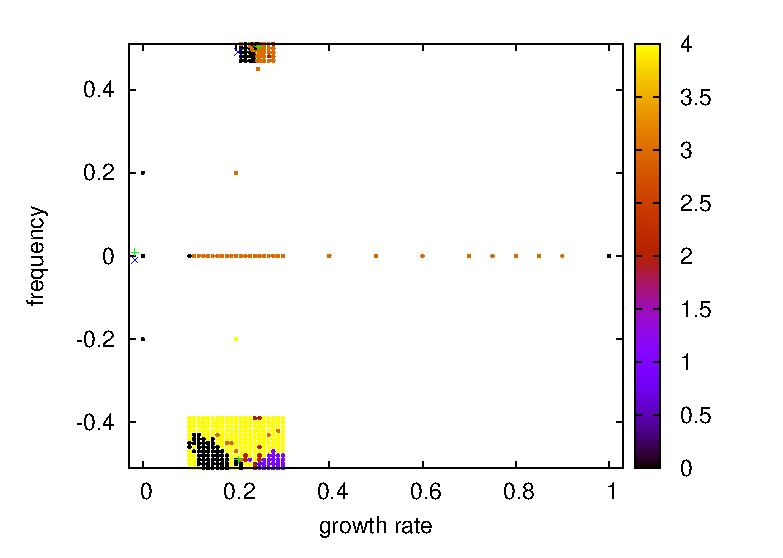
\includegraphics[width=0.8\textwidth]{TargetsA}
    \caption{\label{fig:eivtargetsa} A scan over the target values searching for eigenvalue with largest magnitude, with harmonic extraction.
      Scan along \name{freq = 0}, some of the other two scans can also be
      seen.
      For the meaning of the symbols please refer to the caption of fig.
      \ref{fig:eivtargets1}.}
  \end{center}
\end{figure}

If you just want to find the fastest growing
eigenmode, there is not much variation in the speed a solution is found.
 In the examples here, 900-1000 iterations were
needed (if a mode was found at all). This is different though for the violet points,
 which needed 6000-8000 iterations.
For the second eigenvalue the situation is
quite samilar. It is typically found 100-150 iterations after the first one in
the case of fig. \ref{fig:eivtargets1}, whereas for fig. \ref{fig:eivtargets2}
it is found even quicker. Finding a third (stable) eigenvalue may then take several thousand further iterations.  
Wasting computing time unnecessarily can be avoided by setting a suitable value for max_iterations,
setting \name{max_seconds} or by observing the log and placing a \name{gkw.stop} if desired.\\

Robustness and speed of the solver are very dependent on the initial condition.
We found \name{finit='cosine4'} to be a good choice, but when
doing a parameter scan, it can also be useful to restart with the output of the previous
run.  The batch launcher \scripts{gkwnlin} provides the feature (\name{-restart_chain}) for doing 
this.

The diagnostic output is only written when the solver finishes,
i.e. as soon as the requested number of eigenvalues is found, the
maximum number of iterations is reached, 
or the solver stops due to \name{gkw.stop} or \name{max_seconds}. 
No diagnostic output is produced if the code is killed preliminarly by the queuing system.

The diagnostic output differs from the output obtained with \name{method = 'EXP'}.
The main difference is that eigenmode index takes the place of the time in time-dependent datasets.\\
 For example, the first line in \File{fluxes.dat} will contain
the fluxes computed for the first eigenmode, the second line those for
the second eigenmode, and so on.

You will also notice that instead of a single \File{parallel.dat} or restart file, one for each found eigenmode is produced.

Furthermore, there is an diagnostic output \File{eigenvalues} that contains the growth
rate and frequency determined by {\sc slepc} (first column acts as an index).

If eigenvalues are found, you should check that these belong to a
reasonable, physical mode. If
the eigenvalues computed by the \name{diagnos_growth_freq} diagnostics and the one
determined by slepc (found in \File{eigenvalues.dat}) differ this is a sign
that the result may be unphysical. 
Another possibility to check this is to plot the mode structure.
Note that some of the eigenvalues found could be physical while others
are not. In particular for stable eigenmodes, different parallel decompositions 
 may result in different eigenmodes being found, 

%-----------------------------------------------------------------------------

\section{Technical details}
\label{sec:eivtechdetails}
The eigenvalue solver in {\sc gkw} is mainly a interface for the library
 {\sc slepc} (which relies on {\sc petsc}).

Most parameters of the \name{eiv_integration} namelist are directly passed down to
 {\sc slepc}.

Note that no matrix is given to {\sc slepc}, as the so called matrix-free approach
is used. This means instead of a matrix we define the action of the matrix
on a vector via a function, provided to {\sc slepc}.
%This approach is used as the actual matrix is not available.
Depending on the settings in the input file, either \code{exp_integration} 
(\name{mat_vec_routine = 1}) is used
to determine the result of the matrix vector multiplication or just the subroutine
\code{calculate_rhs} (\name{mat_vec_routine = 2}).

%-----------------------------------------------------------------------------

\subsection{The actual eigenvalue problem}
\label{subsec:eivproblem}
In general an eigenvalue problem is formulated as
\begin{equation}
  A x = \lambda x, \label{eq:eivgen}
\end{equation}
where $A$ is the operator of the problem and $\lambda$ is the (complex)
eigenvalue.
The \code{exp_integration()} routine computes
\begin{equation}
  f_{t+1} = f_{t} + dt A f_{t} + dt B \phi
\end{equation}
\begin{equation}
  0 = C f_{t} + D \phi
\end{equation}
where $A$, $B$, $C$ and $D$ are matrices and the vectors $f$ and $\phi$
represent all the fields that may be present in the simulation.
Note that GKW works with a vector \code{fdisi} = ($f, \phi$).

In principle it is possible to solve the field equation for $\phi$ and insert
it into the evolution equation to get
\begin{equation}
  f_{t+1} = f{t} + dt A f_{t} - dt B D^{-1} C f_{t}.
\end{equation}
The disadvantage of this approach is, that the inversion of the matrix $D$
and the matrix matrix multiplication most probably would destroy the sparsity
structure of the complete operator. 
This would make the determination of the eigenvalues much more expensive.
For this reason the actual matrix of this problem is not explicitly formulated.

%-----------------------------------------------------------------------------

\subsection{Transformation between eigenvalue and growth rate/frequency}
\label{subsec:eivtrafoeivgf}
The transformation between the complex eigenvalue computed by SLEPC and the growth
rate and frequency in terms of GKW can be derived as follows.
In comparison to the eigenvalue problem formulated in \eqref{eq:eivgen}, 
the eigenvalue problem in GKW is
\begin{equation}
  l f =  (1 + dt N)^n f
\end{equation}
where $N$ stands for the effective matrix of evolution and field equation and $n$ is \code{naverage}.
Identifying $M$ and $(1 + dt N)^n$ results in
\begin{equation}
  \lambda = (1 + dt N) = l
\end{equation}
\begin{equation}
  \ln \lambda = n \ln l
\end{equation}

\begin{equation}
  \frac{\ln \lambda}{n dt} = \frac{\ln l}{n dt}
\end{equation}
The right hand side of these equation is the same relation as between the
change in the norm and the growth rate in the code. We take this as reason to
propose this as general transformation between the eigenvalue found by slepc and
the growth rate and frequency as commonly used in GKW.

\newcommand{\pder}[2]{\frac{\partial#1}{\partial#2}}
The transformation for the tolerance $a$ is
\begin{align}
	a_{gkw} & = & \sqrt{\left( \pder{\lambda_{gkw}}{\lambda_{slepc}} |\lambda_{slepc}|a_{slepc}\right)^2} \\
	& = & \sqrt{\left( \pder{(\log(\lambda_{slepc})/(n_{average} \Delta t))}{\lambda_{slepc}} |\lambda_{slepc}|a_{slepc}\right)^2} \\
	& = & \sqrt{\left( \frac{1}{n_{average} \Delta t} a_{slepc}\right)^2} \\
	& = & \frac{a_{slepc}}{n_{average} \Delta t}
\end{align}


%-----------------------------------------------------------------------------

\section{\label{sec:eivfaq}FAQ}

\paragraph{What is a good starting point for the parameters?}

For the Ritz extraction
to find the two most unstable modes you could try
\begin{verbatim}
&CONTROL
 fac_dtim_est=0.5, naverage= 1, method= 'EIV', meth= 1,
 read_file = .true., irun = 2   ! to restart from previous dominant mode
 ! using gkwnlin -restart_chain
 max_seconds = 10000 ! adjust the runtime
 /
&EIV_INTEGRATION
 max_iterations = 90000
 tolerance=1.0e-4
 number_eigenvalues=2
 type_extraction = 'ritz'
 which_eigenvalues=3 ! search for most unstable modes
 /
\end{verbatim}
It seems that the timestep must not be larger than that required for explicit time integration
but that setting a very small timestep makes the convergence take longer.
Setting the tolerance too small can also cause convergence to take longer, and can even prevent finding
the correct modes.

For the harmonic extraction, you can try the following.
\begin{verbatim}
 &CONTROL
 fac_dtim_est=0.5,
 naverage= 1,
 method= 'EIV',
 meth= 1,
 max_seconds = 10000 ! adjust the runtime
 /
 &EIV_INTEGRATION
 max_iterations = 90000
 tolerance = 1.0e-4
 type_extraction = 'harmonic'
 number_eigenvalues = 2
 nr_column_vec      = 20
 mat_vec_routine    = 1
 which_eigenvalues  = 8 ! look for eigenvalues near the target growthrate
 growthrate = 0.5000 
 freq = 0.0000
 /
 &SPCGENERAL
 finit="cosine4"
 /
 \end{verbatim}
If you increase \code{number_eigenvalues} you may also have to increase
\code{nr_column_vec}.

\paragraph{Does \code{nr_column_vec = 0} (letting 'PETSC_DECIDE') work?}

From the scan done over the size of the subspace (see fig. \ref{fig:eivharmonicncv}
we would expect, that it should work well for at least \code{number_eigenvalues = 1-2}.
For bigger values it might be not optimal.\\
Experience shows that even for \code{number_eigenvalues = 15} eigenvalues 
were found.

\paragraph{I try to compile in single precision/default real but
eiv_integration.F90 fails./Testcases fail after I fix the errors.}
You probably have to configure {\sc pets}c/{\sc slep}c
 \code{--with-precision=single} (as of 3.6.2). It has not been checked if the
code then actually works, though.
Just fixing the bugs that prevent compiling is not enough as there will still
be a type mismatch between the vectors used by {\sc slep}c and the arrays
used by gkw.

\paragraph{How Do I find the number of iterations at which an eigenmode was found?}
You can find this information in the screen output as soon as
converged modes are found. You may stop the run at any time
by creating a \name{gkw.stop} file.

% \paragraph{Is there a way to output eigenmodes as they are found, instead
% of waiting until the end or the maximum number of iterations ?}

% \paragraph{Doesn't the optimal nr_colum_vec increase with the problem size ?}

% related to auctex mode and latex-preview-mode in Emacs:
%%% Local Variables:
%%% mode: latex
%%% TeX-master: "doc"
%%% End:

\chapter{The non-spectral and global version of the code}

This chapter discusses the non-spectral and global version of the code.  (Work in 
progress) 

Non-spectral \index{Non-spectral} here refers to the treatment of the radial direction through the use of finite 
difference methods, and is switched on through the switch 
\begin{equation}
\hbox{\tt spectral_radius = .false.}
\end{equation}
in the control namelist. The non-spectral representation can be used both in the local limit
(which we will refer to as flux-tube) as well as in the global case. 
The term \emph{global} \index{Global simulations} is used as synonym for allowing for
profile effects, i.e. allowing plasma and geometry parameters to 
be a function of the radius. A global run is selected by setting 
\begin{equation}
\hbox{\tt flux_tube = .false.}
\end{equation}
in the \name{CONTROL} namelist. Naturally, global simulations can only be performed with a non-spectral 
representation. Global simulations can still be $\delta f$ simulations, i.e. the perturbed distribution 
function can be assumed small compared to the background. In this case energy is not conserved since
the parallel velocity nonlinearity (cf. section \ref{sec:velocity-nonlinearity})is neglected. Energy conserving simulations will be referred to as 
full-f simulations below\index{full-f simulations}, and can be run setting 
\begin{equation}
\hbox{\tt lpar_vel_nl = .true.} 
\end{equation}
in the \name{CONTROL} namelist.  

Two points should be noted: First, although you can run with the parallel velocity nonlinearity 
in a flux-tube run, there is no point since the expansion around a local flux surface means that energy 
cannot be conserved (It can easily be shown that the integrated kinetic energy in the perturbed 
distribution is always zero in the local limit, while the integrated energy in the field must be postive. 
The two can then not balance each other). 
Therefore, global full-f, global $\delta f$, and local $\delta f$ make sense, but local 
full-f does not, unless one wants to study some distinct property of the velocity nonlinearity. 

Second, care must also be taken using global $\delta f$. The turbulence will lead to a 
rapid profile evolution that is represented by the perturbed distribution. The condition 
$\delta f = {\cal O}[ \rho_* F_M ]$ is then easily violated. 
One way to keep $\delta f$ small is through the Krook operator (see the section below), which damps the 
perturbed distribution on a specified timescale and acts through this damping as a source / sink of energy. 
But even with the use of the Krook operator the ordering is not necessarily satisfied. 

\section{Complete Set of Equations}
\label{sec:global-compl-set-equat}


With the new normalization as described in \ref{sec:normalisation-global-specialities} the equations of motion are
\begin{equation}
\label{eqs:global-complete-set}
\pd{g}{t} = {\rm I} + {\rm II} + {\rm III} + {\rm IV} + {\rm V} + {\rm VI}+ {\rm VII}+ {\rm VIII},
\end{equation}
with 
\pagebreak
%\abovedisplayskip
%\belowdisplayskip
%\begin{small}
\begin{align}
\label{eq:gI}{\rm I} &= - v_\parallel {\bf b} \cdot \nabla f \rightarrow - w v_{\parallel} {\cal F} \pd{f}{s}, \\
\noalign{\vskip 0.4 truecm} 
%
\label{eq:gII}{\rm II} &= - {\bf v}_D \cdot \nabla f \rightarrow \cr 
\noalign{\vskip 0.4 truecm} 
& \hspace{0.5cm} -\frac{\rho_*}{Z} \left[ T_G E_D {\cal D}^\alpha + T_G v_{\parallel}^2 \beta^\prime  {\cal E}^{\psi \alpha} + 2 m w v_{\parallel}\Omega{\cal
H}^\alpha + m \Omega^2 I^\alpha + Z{\cal E}^{\beta \alpha} \pd{\Phi}{x_\beta}\right] 
\pd{ f}{x_\alpha}  \\
\noalign{\vskip 0.4 truecm} 
%
\label{eq:gnl-term}
{\rm III} &= - {\bf v}_\chi \cdot \nabla g \rightharpoonup - \rho_*^2 \pd{\chi}{x_\beta} 
{\cal E}^{\beta \alpha} \pd{g}{x_\alpha} \\
\noalign{\vskip 0.4 truecm} 
%
\label{eq:gIV}{\rm IV} &= + \frac{\bf b}{ m }\cdot(\mu \nabla B + \nabla \cfen) \pd{ f }{v_\parallel} \rightarrow
w \left(\mu B {\cal G} + \pd{T}{2 T_G} {\cal F} \pd{ {\cal E}_\Omega }{s} \right) 
\pd{  f }{v_{\parallel}},\\
\noalign{\vskip 0.4 truecm} 
%
\label{eq:gV}{\rm V} &= - {\bf v}_\chi \cdot \nabla F_M \rightarrow  
\rho_* \pd{ \chi }{x_\alpha}  
 {\cal E}^{\alpha \psi} \biggl [ \frac{1}{L_n} + E_T \frac{1 }{ L_T} + \biggl ( \frac{2 m w v_{\parallel}}{T} 
 \frac{R B_t }{ B} + \frac{2 m \Omega }{ T} {\cal J} \biggr ) u^\prime + \frac{m \Omega^2 }{ T}{\cal L} \biggr ] F_{M} \\
\noalign{\vskip 0.4 truecm} 
%
\label{eq:gVI}{\rm VI} &= - {\bf v}_D \cdot \nabla F_M \rightarrow  \frac{1 }{ Z} \left[ T_G E_D {\cal D}^\psi + 2 m w v_{\parallel}
\Omega{\cal H}^\psi + m \Omega^2 I^\psi + Z{\cal E}^{s \psi} \pd{ \Phi }{s}\right] \\
\noalign{\vskip 0.4 truecm}
& \hspace{2.3cm} \times \biggl [ \frac{1 }{ L_n} + E_T \frac{1 }{ L_T} + \biggl ( \frac{2 m w v_{\parallel}}{ T} 
 \frac{R B_t }{ B} + \frac{2 m \Omega }{ T} {\cal J} \biggr ) u^\prime + \frac{m \Omega^2 }{ T}{\cal L} \biggr ] F_{M} ,\\ 
\noalign{\vskip 0.4 truecm} 
%
\label{eq:gVII}{\rm VII} &= - \frac{Z e }{ T} v_\parallel {\bf b} \cdot \nabla \langle \phi \rangle F_M \rightarrow - 
\frac{Z }{ T} w v_{\parallel} {\cal F} \pd{ {\langle \phi \rangle} }{s} F_{M} ,\\
\noalign{\vskip 0.4 truecm} 
%
\label{eq:gVIII}{\rm VIII} &= - \frac{Z e }{ T}{\bf v}_D \cdot \nabla \langle \phi \rangle F_M  \rightarrow \cr 
\noalign{\vskip 0.4 truecm} 
& \hspace{0.2cm} - \frac{\rho_* }{ T} \left[ T_G E_D {\cal D}^\alpha + T_G \beta^\prime v_{\parallel}^2 {\cal E}^{\psi \alpha} + 
{2 m w}v_{\parallel}\Omega{\cal H}^\alpha + {m\Omega^2 }{\cal I}^\alpha 
+ {Z} {\cal E}^{\beta \alpha} \pd{ \Phi }{x_\beta} \right] 
\pd{ \langle \phi \rangle }{x_\alpha} \, F_{M} \cr 
\noalign{\vskip 0.4 truecm} 
%
\end{align}
Here, all quantities are normalized, i.e. $w$ in these equations 
refers to $w_N$, etc.
Moreover we use the generalised potential 
\begin{equation} 
\chi = {\langle \phi \rangle} - 2 w v_{\parallel} {\langle A_{\parallel} \rangle}  %+ \frac{2 T_G }{ Z} \mu B_{\parallel} 
\end{equation} 
and 
\begin{equation} 
g = f + \frac{2 Z }{ T} w v_{\parallel} {\langle A_{\parallel} \rangle} F_{M}, 
\end{equation}
\begin{equation}
E_D = v_{\parallel}^2 + \mu B , \qquad 
E_T = \frac{T }{ T_G} \left [ v_{\parallel}^2 + 2 \mu B  + {\cal E}_\Omega \right ]  - \frac{3}{ 2} .
\end{equation}
\begin{equation} 
\frac{1 }{ L_N} \equiv - \frac{1 }{ n}\pd{ n }{\psi} \qquad 
\frac{1 }{ L_T} \equiv - \frac{1 }{ T}\pd{ T }{\psi} \qquad 
u^\prime      \equiv - \pd{ \omega_\phi }{\psi} 
\end{equation}
The equations above apply to each of the species individually. 

In the equations the spatial derivatives of the perturbed distribution function appear, and the Einstein summation convention has been used. 
To shorten the notation, the sum over $\alpha$ also includes $\alpha = s$.
The directions $s$ and $\psi$ are treated in position space, i.e. finite differences discretise  $\pd{}{x^\alpha}$.
\begin{align}
  \pd{}{\psi} &= \frac{1}{R_\tref} \pd{}{\psi_N} \\
\pd{}{s} &\sim \orderof(1)\text{$s$ is naturally normalised}
\label{eq:global-s-normalisation}
\end{align}
Note that the ordering nevertheless assumes that flucuations vary on the lengthscale $\rho_\tref$, not $R_\tref$.
\begin{align}
\pd{\hat f_N}{\psi}
&= \frac{1}{\rho_\tref} \pd{\hat f_N}{\psi_N} 
= \frac{R_\tref}{\rho_\tref} \frac{1}{R_\tref}\pd{\hat f_N}{\psi_N} \\
&= \frac{1}{\rho_*}\left(\pd{\hat f_N}{\psi}\right)_N
\label{eq:global-dpsi-normalisation}
\end{align}
For the $\zeta$ coordinate principally we have
\begin{align}
  \pd{}{\zeta} \sim \orderof(1)\text{$\zeta$ is naturally normalised}
\end{align}
but actually $\zeta$-derivatives only of fluctuating quantities appear
(not of the background - this is tokamak-only)
where the ordering assumes
\begin{align}
  \pd{\hat f_N}{\zeta} = \frac{1}{\rho_*}\left(\pd{\hat f_N}{\zeta}\right)_N
\end{align}
In the code, the $\zeta$ grid is treated in spectral representation, and we write
\begin{align} 
\pd{\hat f_N}{\zeta} &\rightarrow {\rm i} k_\zeta \hat f_N = {\rm i} \frac{1}{\rho_*}k_{\zeta N} \hat f_N
\label{eq:global-kzeta-normalisation}
\\
\left(\pd{\hat f_N}{\zeta}\right)_N &\rightarrow {\rm i} k_{\zeta N} \hat f_N
\end{align}

In contrast to the perpendicular ones \eqref{eq:global-dpsi-normalisation} and \eqref{eq:global-kzeta-normalisation}, the terms containing
$s$-derivatives \eqref{eq:global-s-normalisation} are $\rho_*$ smaller than the derivatives
perpendicular to the magnetic field.
For this reason they are usually neglected on the level of the evolution equations (although this may break physical system properties, see section \ref{sec:velocity-nonlinearity}).
These ``higher order $\rho_*$ terms''  have been studied in connection with momentum transport in Ref.~\cite{SUN13}, and must be explicitly switched on through the input file, to involve them.

\section{Missing implementation}
\label{sec:global-missing}

Not all physics which is available for flux-tube systems in GKW has already been implemented for the global case or makes sense.

\subsection*{Plasma Rotation}
\label{sec:global-plasma-rotation}

The frame rotation $\Omega$ is in both flux-tube and global case not a function of the radius. 
This is more than just a choice. 
The beauty of a corotating frame in the flux-tube case lies in the fact that rotational 
phenomena can be more clearly adressed when the background rotation is zero with respect to the frame.

Now, if in the global case the frame rotation is a function of the radius, one could have the idea to choose a frame which also rotates differentially.
The issue with such a frame is, that in general two stationary points in the co-moving frame 
shear apart in the laboratory frame. 
In short, the metric tensor would be a function of time, which is highly undesirable.

By choosing a frame which rotates with at single frequency $\Omega$, the frame is not a comoving frame everywhere.
Such a frame is equivalent to the laboratory frame and will not simplify the examination of the system.

The co-moving frame description of the rotation is, therefore, useful for the flux tube case, but less so 
for the global case. 
The use of $\Omega$ in the global case is allowed, but the implementation is not entirely consistent (the 
${\cal E}_\Omega$ quantity, for instance, is not a function of the radius). 
The user is therefore strongly discouraged from using the plasma rotation $\Omega$ in the global case. 
Momentum fluxes due to the $u^\prime$ however can be calculated. 
In the future a rotation profile will be implemented through a shift of the perturbed distribution, rather than 
a coordinate transformation. 


\section{Krook operator}
\label{seckrookoperator}
\index{Krook operator} 
In a global run the profiles relax. Without any sources or sinks this leads 
to a decay of the turbulence since it is no longer driven. One of the methods
to obtain a 'stationary' turbulence run is to enable the Krook operator via the 
settings in the \texttt{KROOK} namelist. The implementation for \texttt{krook_option=1} 
picks an operator which conserves density and parallel velocity, but not 
energy. \\
The Krook operator $\mathcal{C}_K$ takes the shape of a source or damping term in the gyrokinetic equation.
\begin{align}
  \pd{ f (\mathbf{X}, v_\parallel,\mu)}{ t} + ... &= \mathcal{C}_K
\end{align}
% Below, the change of a quantity due to the Krook operator will be denoted by $|_K$, like this
% \begin{align}
%   \pd{ f (\mathbf{X}, v_\parallel,\mu)}{ t}\biggr|_K &= \mathcal{C}_K
% \end{align}

In the following, the operator implemented for \texttt{krook_option=1} is described. 
First the density moment is calculated and stored in the array \texttt{sss} 
\begin{equation}
\mathtt{sss}  = \tilde n = \int f \, {\rm d}^3 {\bf v}
\end{equation}
FIXME this was not the density moment...?|
This density moment is used in the calculation of the damping term 
\begin{equation}
%\pd{ f (v_\parallel,\mu)}{ t} \biggr \vert_{K}  
\mathcal{C}_K
= - \gamma_K \biggl [   
\frac{1 }{ 2} [ f(v_\parallel,\mu) + f(-v_\parallel,\mu)] -  \tilde n \bar F_M(v_\parallel,\mu) \biggr ] 
\label{eq:krook-option1}
\end{equation}
The Maxwellian $\bar F_M$ here is not precisely identical to $F_M$ from \eqref{eq:maxwell}, but defined such that it satisfies 
\begin{equation}
\int \bar F_M \, {\rm d}^3 {\bf v} = 1 \qquad \int \frac{1}{ 2} m v^2 \bar F_M \, {\rm d}^3 {\bf v} = \frac{3 }{ 2} T 
\end{equation}
where T is the local background Temperature. 
Integration of \eqref{eq:krook-option1} over velocity space shows that this operator does not constitute a source or sink of particles.
\begin{align}
\pd{}{ t} \biggr \vert_{K} \int f \, {\rm d}^3 {\bf v} =
 \int \mathcal{C}_K \, {\rm d}^3 {\bf v}
 &=   - \gamma_K\int \, {\rm d}^3 {\bf v}  \biggl [   
\frac{1 }{ 2}[f(v_\parallel,\mu) + f(-v_\parallel,\mu)] -  \tilde n \bar F_M(v_\parallel,\mu) \biggr ] 
\nonumber\\
&=   - \gamma_K\biggl [   
\frac{1 }{ 2}\int \, {\rm d}^3 {\bf v}   f(v_\parallel,\mu) 
+\frac{1 }{ 2} \int \, {\rm d}^3 {\bf v}  f(-v_\parallel,\mu)] 
-  \int \, {\rm d}^3 {\bf v}  \tilde n \bar F_M(v_\parallel,\mu) \biggr ] 
\nonumber\\
&=   - \gamma_K [ \tilde n  - \tilde n] 
\nonumber\\
&= 0
\end{align}
FIXME for me this is not 0, so I suppose $\tilde n$ is not supposed to be a density moment?|g
That is, under the action of the term \eqref{eq:krook-option1} density is locally conserved. 

The parallel velocity moment is
\begin{equation}
%\pd{}{ t} \biggr \vert_{K} \int v_\parallel f \, {\rm d}^3 {\bf v} = 0 
\int v_\parallel \mathcal{C}_K \, {\rm d}^3 {\bf v} = 0 
\end{equation}
i.e. also the parallel momentum is locally conserved. Of course, the energy is not 
\begin{equation}
%\pd{}{ t} \biggr \vert_{K} \int \frac{1 }{ 2 } m v^2 f {\rm d}^3 {\bf v}  = 
\int \frac{1 }{ 2 } m v^2 \mathcal{C}_K {\rm d}^3 {\bf v}  = 
- \gamma_K \int \left [ \frac{1 }{ 2} m v^2 - \frac{3 }{ 2} T_0 \right ] f \, {\rm d}^3 {\bf v} 
\end{equation}
Since density is conserved the perturbed distribution can not be uniformly (in velocity space) damped. 
The expression above makes clear that the distribution function is reduced for energies more than the 
thermal energy of the bulk, whereas it is growing for smaller energies. 

\texttt{krook_option=3} is similar to the above apart from the lack of velocity space symmetrisation, i.e
\begin{equation}
\pd{ f (v_\parallel,\mu)}{ t} \biggr \vert_{K}  = - \gamma_K \biggl [   
\frac{1 }{ 2} [ f(v_\parallel,mu)  -  \tilde n \bar F_M(v_\parallel,\mu) \biggr ]. 
\end{equation}
This version does not conserve the parallel momentum and damps away any parallel flows.

\texttt{krook_option=4} is a hybrid of these two.  The momentum conserving operator is applied to all non-zero toroidal modes, while the parallel flow damping operator is applied to the $n=0$ mode (the damping rate can be modified by a prefactor gamkpre in the input file) so the perturbed equilibrium toroidal flow is damped away without modifying heavily the turbulence.

\section{Profile functions in GKW}
\label{secprofilefunctions}
\index{Profile functions} 
In the global version one can choose various analytic profiles through the 
switches '\name{dens_prof_type}' and '\name{temp_prof_type}' in the 
\name{SPECIES} namelist. Allowed are at 
present the option '\name{const}', '\name{cosh2}', '\name{tanh}', 
'\name{exp_tanh}', '\name{orb}', '\name{orb3}', '\name{exp_poly3}', '\name{exp_poly6}' as well as '\name{file}'. 
Specifying the latter will make GKW read the profile data from the file \name{input.prof}, whereas all the others denote an analytic expression for the respective profile.

The parameters needed for the analytic profile expression are given 
in the arrays 'dens_prof_coef' and 'temp_prof_coef'. At present a maximum 
of five parameters is available. 

Below the quantity $G$ stands for either density or temperature and $G'$ is its normalised gradient.
\begin{equation}
G' = \frac{1 }{ G} \d{ G }{ \psi} 
\end{equation}

Besides the profiles of density and temperature one can also specify the 
$q$ profile. To select a specific profile one sets the \name{prof_type} 
option in the \name{GEOM} namelist. The magnetic shear is calculated 
consistently with the profile specified. Valid options are at present: 
'\name{parabolic}', '\name{parabolic2}', '\name{orb}', '\name{wesson}', 
'\name{rexp}', '\name{mishchenko}'. The parameters needed for the analytic $q$ 
profile are given to the code through \name{qprof_coef} array in the namelist \name{GEOM}.

The figures \ref{comparisonProfile} and \ref{comparisonDprofile} show some of
the temperature/density profiles and the corresponding gradient length, respectively.
All the profiles use the same parameter set $(1.0, 5.0, 0.15, 0.1, 0.1$ and
thus might not be physical.\\
Examples for the safety factor and the corresponding shear are shown in fig.~\ref{comparisonQprofile}
and \ref{comparisonSprofile}, respectively. All the profiles use the same
parameter set $(0.9, 5, 3)$ and thus might not be physical.

\begin{figure}
  \begin{center}
    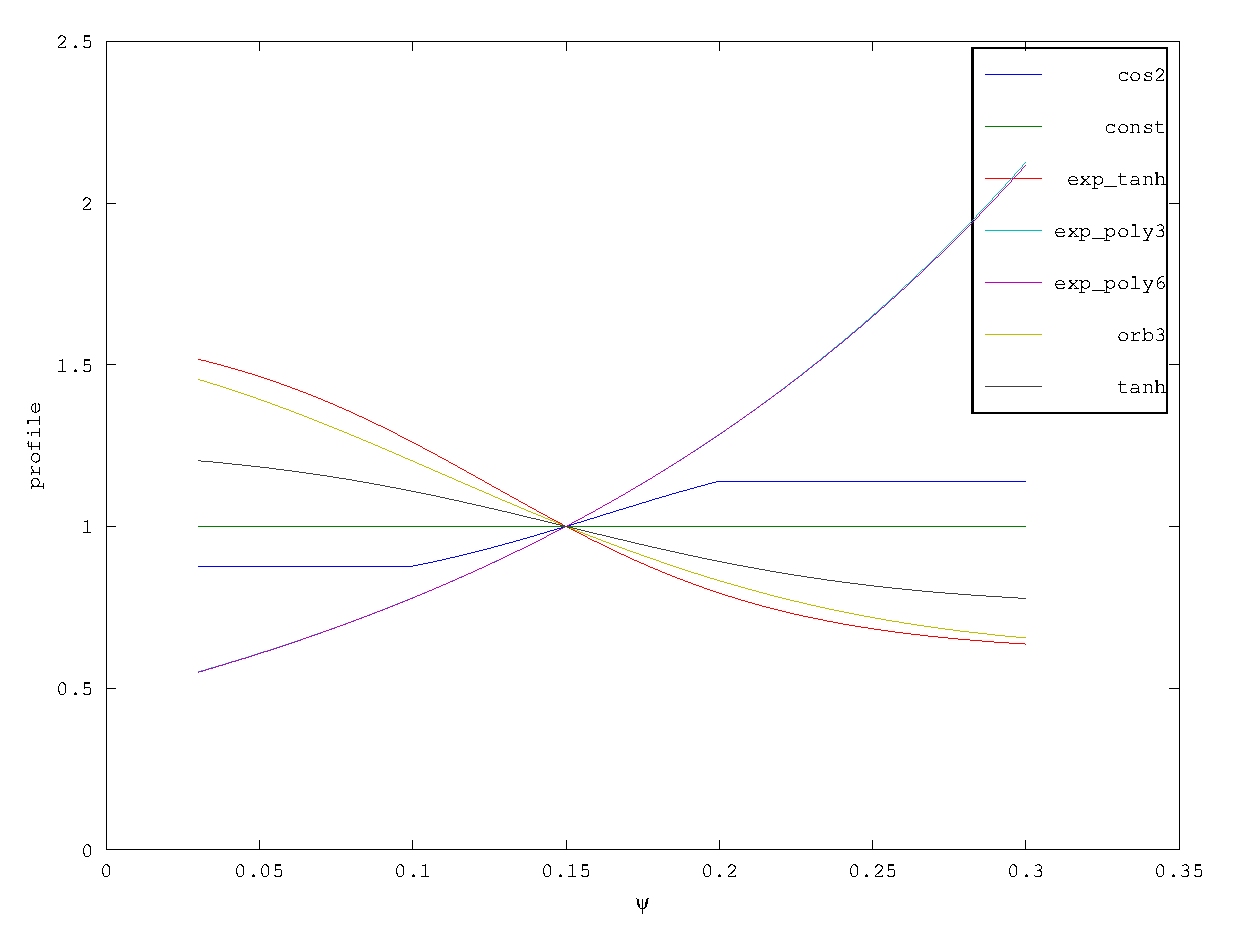
\includegraphics[width=0.8\textwidth]{comparisonProfile}
    \caption{\label{comparisonProfile}Comparsion of some possible profiles for density/temperature. All use the same set of parameters (see text) and thus might be nonphysical.}
  \end{center}
\end{figure}

\begin{figure}
  \begin{center}
    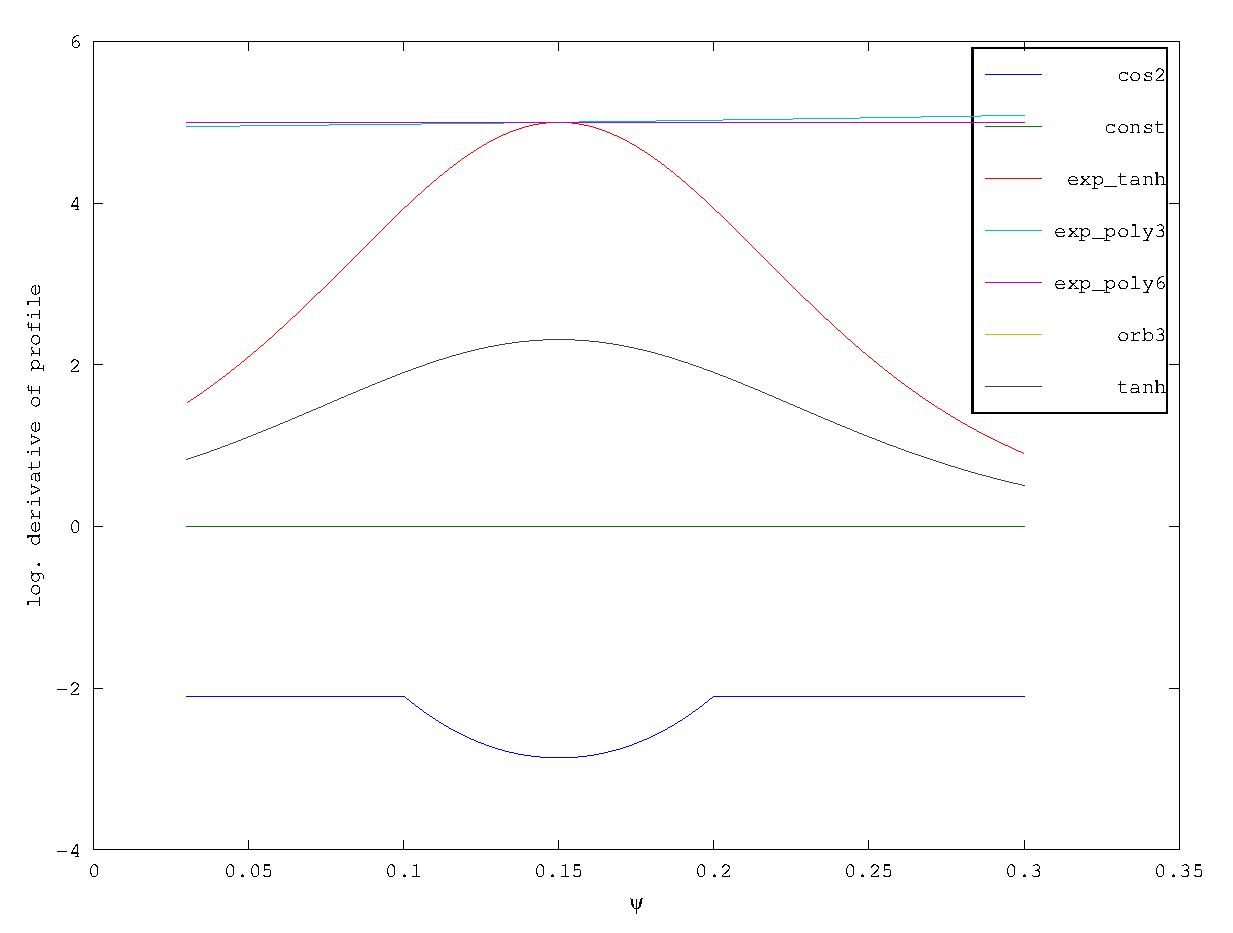
\includegraphics[width=0.8\textwidth]{comparisonDprofile}
    \caption{\label{comparisonDprofile}Comparsion the gradients length of some possible profiles for density/temperature. All use the same set of parameters (see text) and thus might be nonphysical.}
  \end{center}
\end{figure}

\begin{figure}
  \begin{center}
    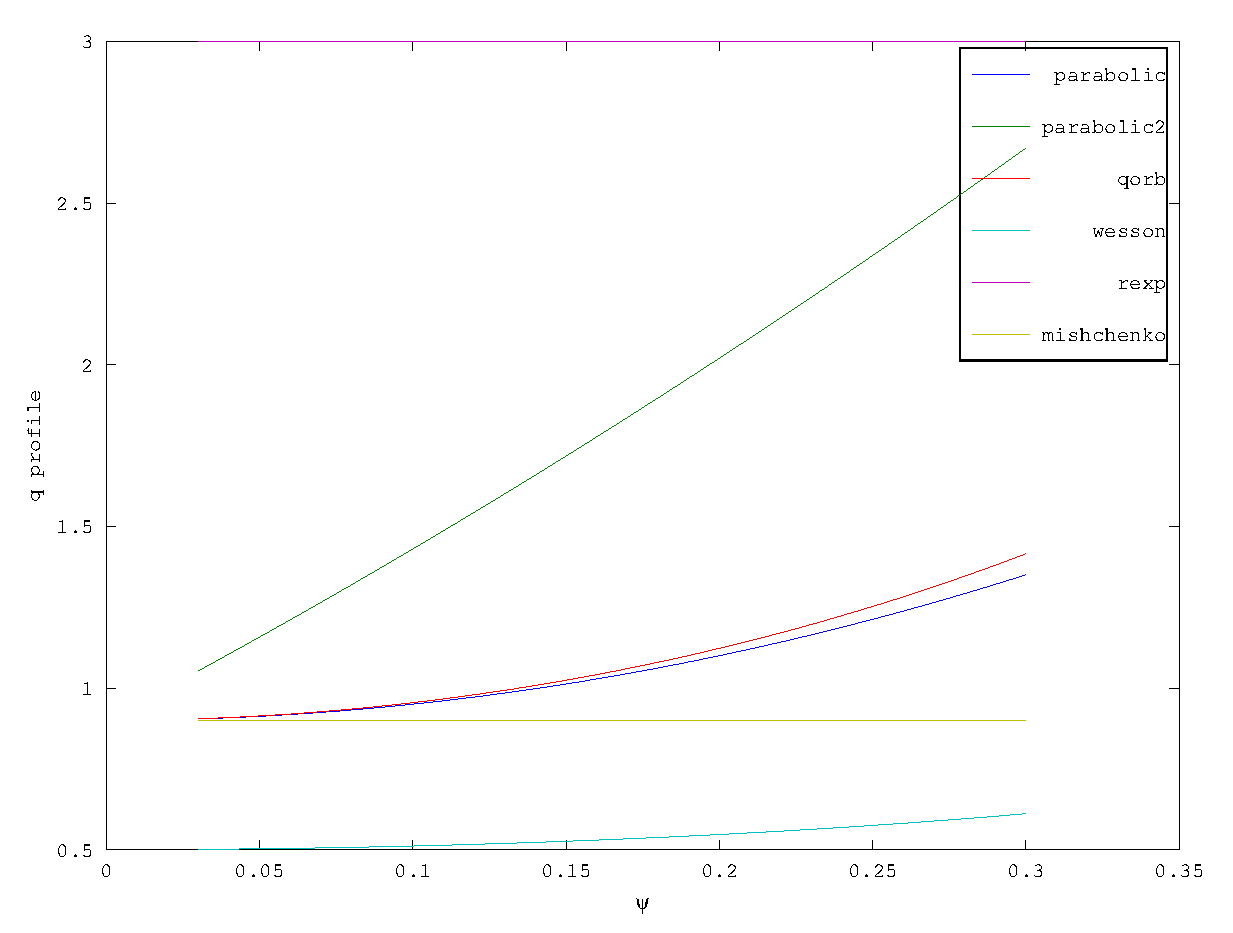
\includegraphics[width=0.8\textwidth]{comparisonQprofile}
    \caption{\label{comparisonQprofile}Comparison of some possible safety factor profiles. All use the same set of parameters (see text) and thus might be nonphysical.}
  \end{center}
\end{figure}

\begin{figure}
  \begin{center}
    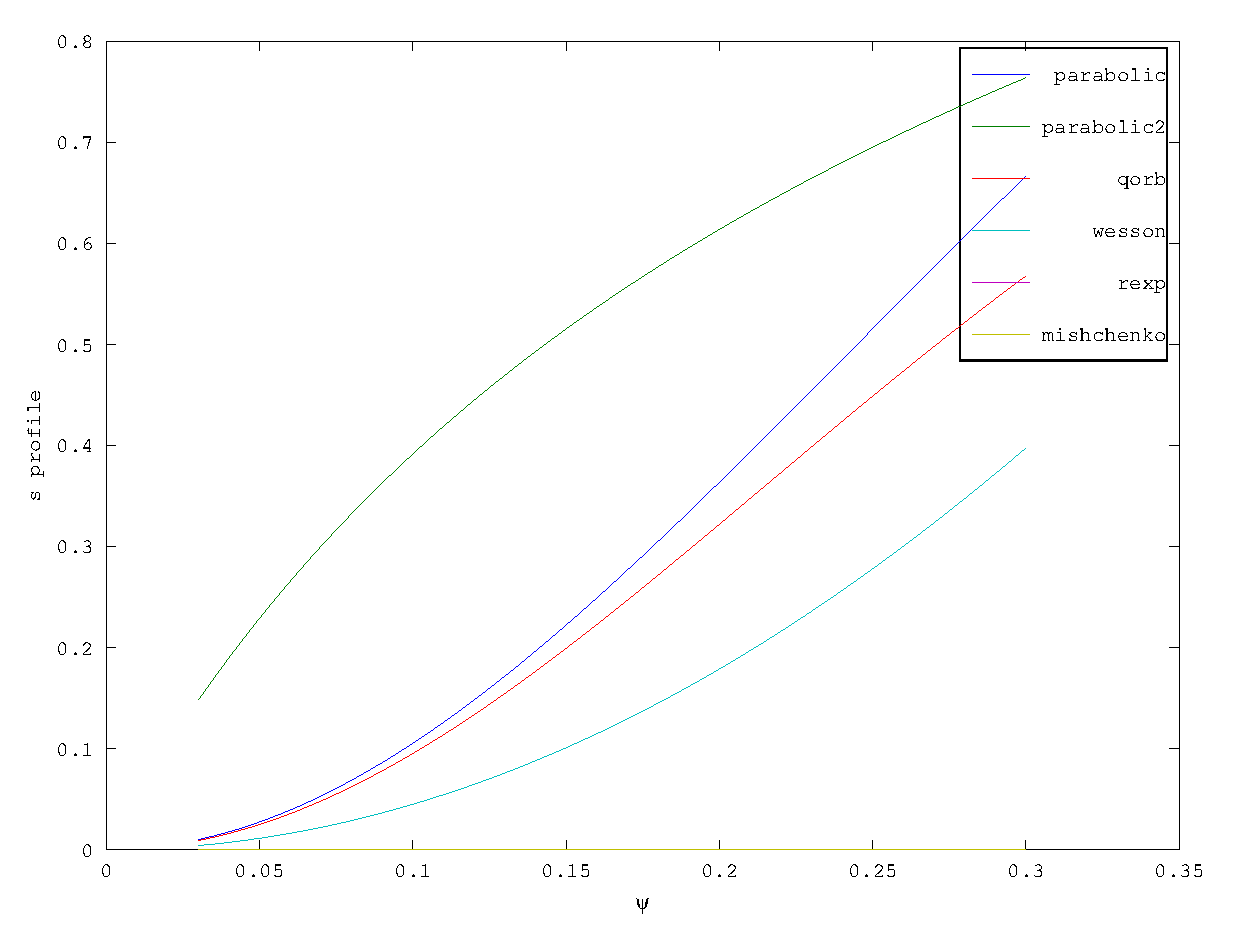
\includegraphics[width=0.8\textwidth]{comparisonSprofile}
    \caption{\label{comparisonSprofile}Comparison of the shear for some possible safety factor profiles. All use the same set of parameters (see text) and thus might be nonphysical.}
  \end{center}
\end{figure}


\subsection{Density/Temperature profile option: cosh2}
Allows to have a plateau like gradient profile, i.e. almost constant in the
middle and going to zero at the border.

\begin{eqnarray*}
G_0    = {\rm dens\_prof\_coef}(1)   &\hbox{the density / temperature at $x = X_0$} \cr
R/L_G  = {\rm dens\_prof\_coef}(2)   &\hbox{gradient length R/L_G at $x = X_0$}\cr
X_0    = {\rm dens\_prof\_coef}(3)   &\hbox{Radial location of the maximum gradient}\cr
w      = {\rm dens\_prof\_coef}(4)   &\hbox{the normalized width of the plateau $\Delta x / R_0$}\cr
\Delta = {\rm dens\_prof\_coef}(5)   &\hbox{Width that determines the rise of the $R/L_T$ profile}
\end{eqnarray*}
\begin{equation}
X = {\rm min}({\rm max}(X_0-w/2,\psi),X_0+w/2.)  
\end{equation}
\begin{equation}
G = G_0 \exp\biggl [ -\frac{R }{ L_G} (X-X_0) + \frac{R}{ L_G} \Delta \tanh \biggl ( \frac{X - X_0 + w / 2 }{ 
\Delta} \biggr ) + \frac{R}{ L_G} \Delta \tanh \biggl ( \frac{X - X_0 - w / 2 }{ 
\Delta} \biggr ) \biggr ] 
\end{equation}
\begin{equation}
G^\prime = \frac{R}{ L_G} \biggl ( 1 - \frac{1 }{ \cosh^2 ((X - X_0 + w / 2)/\Delta)} - 
 \frac{1 }{ \cosh^2 ((X - X_0 - w / 2)/\Delta)}\biggr ) 
\end{equation}
\begin{equation}
G_{\rm norm} = G_0   
\end{equation}

\subsection{Density/Temperature profile option: 'const'} 

\begin{eqnarray*}
G_0    = {\rm dens\_prof\_coef}(1)   &\hbox{the density / temperature }
\end{eqnarray*} 
\begin{equation}
G = G_0 
\end{equation}
\begin{equation}
G^\prime = 0
\end{equation}
\begin{equation}
G_{\rm norm} = G_0 
\end{equation}

\subsection{Density/Temperature profile option: 'exp_tanh'}

\begin{eqnarray*}
G_0    = {\rm dens\_prof\_coef}(1)   &\hbox{the density / temperature at $x = X_0$} \cr
R/L_G  = {\rm dens\_prof\_coef}(2)   &\hbox{gradient length R/L_G at $x = X_0$}\cr
X_0    = {\rm dens\_prof\_coef}(3)   &\hbox{Radial location of the maximum gradient}\cr
w      = {\rm dens\_prof\_coef}(4)   &\hbox{the normalized width of the gradient profile $\Delta x / R_0$}\cr
\end{eqnarray*} 
\begin{equation}
G = G_0 \exp \biggl ( - \frac{R}{ L_G} w \tanh \biggl ( \frac{\psi-X_0 }{ w} \biggr ) \biggr ) 
\end{equation}
\begin{equation}
G^\prime = \frac{R }{ L_G} \frac{1 }{ \cosh^2 ((\psi-X_0)/w)}
\end{equation}
\begin{equation}
G_{norm} = G_0
\end{equation}

\subsection{Density/Temperature profile option: '1_m_exp_tanh'}
\begin{eqnarray*}
G_0    = {\rm dens\_prof\_coef}(1)   &\hbox{the density / temperature at $x = X_0$} \cr
R/L_G  = {\rm dens\_prof\_coef}(2)   &\hbox{gradient length R/L_G at $x = X_0$}\cr
X_0    = {\rm dens\_prof\_coef}(3)   &\hbox{Radial location of the maximum gradient}\cr
w      = {\rm dens\_prof\_coef}(4)   &\hbox{the normalized width of the gradient profile $\Delta x / R_0$}\cr
\end{eqnarray*}
\begin{equation}
G = 1 - G_0 \exp \biggl ( - \frac{R}{L_G} w \tanh \biggl ( \frac{\psi-X_0}{w} \biggr ) \biggr )
\end{equation}
\begin{equation}
G^\prime = \frac{R}{L_G} \frac{1}{\cosh^2 \frac{\psi-X_0}{w}}
\end{equation}
\begin{equation}
G_{norm} = 1 - G_0
\end{equation}

\subsection{Density/Temperature profile option: exp_poly3}

Results in a quadratic profile of the gradient length. Limiting cases of linear 
(for a = 0) and constant (for a=0 and b=0) are included. Some care has to be taken 
to get physical profiles. To get a gradient length that is positive over the whole range, 
the inequality $b^2 < 4a$ has to be fullfilled.
\begin{eqnarray*}
G_0    = {\rm dens\_prof\_coef}(1)   &\hbox{the density / temperature at $x = X_0$} \cr
R/L_G  = {\rm dens\_prof\_coef}(2)   &\hbox{gradient length R/L_G at $x = X_0$}\cr
X_0    = {\rm dens\_prof\_coef}(3)   &\hbox{Radial location of the maximum gradient}\cr
a      = {\rm dens\_prof\_coef}(4)   &\hbox{constant for the quadratic term}\cr
b      = {\rm dens\_prof\_coef}(5)   &\hbox{constant for the linear term}
\end{eqnarray*}
\begin{equation}
G = G_0  \exp \left[ - \frac{R }{ L_G} \left(  \frac{a}{3} (\psi - X_0)^3
+ \frac{b}{2} (\psi - X_0)^2  + (\psi - X_0) \right) \right]
\end{equation}
\begin{equation}
G^\prime = \frac{R }{ L_G} \left[ a (\psi - X_0)^2 + b (\psi - X_0) + 1 \right]
\end{equation}
\begin{equation}
G_{\rm norm} = G_0 
\end{equation}

\subsection{Density/Temperature profile option: exp_poly6}

Results in a fifth and third order term as well as a constant for the
gradient length.
\begin{eqnarray*}
G_0    = {\rm dens\_prof\_coef}(1)   &\hbox{the density / temperature at $x = X_0$} \cr
R/L_G  = {\rm dens\_prof\_coef}(2)   &\hbox{gradient length R/L_G at $x = X_0$}\cr
X_0    = {\rm dens\_prof\_coef}(3)   &\hbox{Radial location of the maximum gradient}\cr
a      = {\rm dens\_prof\_coef}(4)   &\hbox{constant for the fifth order term}\cr
b      = {\rm dens\_prof\_coef}(5)   &\hbox{constant for the third order term}
\end{eqnarray*}
\begin{equation}
G = G_0 \exp \left[ - \frac{R }{ L_G} \left(  \frac{a}{6} (\psi - X_0)^6
                                          + \frac{b}{4} (\psi - X_0)^4
                                          +             (\psi - X_0) \right) \right]
\end{equation}
\begin{equation}
G^\prime = \frac{R }{ L_G} \left[  a (\psi - X_0)^5
                           +     b (\psi - X_0)^3
                           + 1 \right]
\end{equation}
\begin{equation}
G_{\rm norm} = G_0
\end{equation}

\subsection{Density/Temperature profile option : orb} 

This produces profiles equivalent to one of the options used in ORB5 (NEMORB). 
The calculation is a little more involved because these orb profiles are 
defined as function of a different radial coordinate. 

\begin{eqnarray*}
G_0    = {\rm dens\_prof\_coef}(1)   &\hbox{the density / temperature at $x = X_0$} \cr
R/L_G  = {\rm dens\_prof\_coef}(2)   &\hbox{gradient length R/L_G at $x = X_0$}\cr
X_0    = {\rm dens\_prof\_coef}(3)   &\hbox{Radial location of the maximum gradient}\cr
w      = {\rm dens\_prof\_coef}(4)   &\hbox{Width of the profile}\cr
X_e    = {\rm dens\_prof\_coef}(5)   &\hbox{minor radius of the plasma edge $X_e = a /R_0$}
\end{eqnarray*}
The values of $\bar {q}$ as used in ORB at the edge and in the centre 
\begin{equation} q_a = q(a) \sqrt{1 - X_e^2} \end{equation}
\begin{equation} q_0    = q(0) \end{equation}
Rescale the gradient length to have exactly the input value at the $s_0$ 
coordinate used in ORB
\begin{equation}
\frac{R}{ L_{G*}} = \frac{R/L_G }{ 1 - 1 / \cosh^2(X_0/w)} 
\end{equation}
Calculate the $s$ coordinate used in ORB 
\begin{equation} 
s = \sqrt{\left ( \frac{\log(1 + (q_a - q_0)\psi^2/(q_0 X_e^2)) }{ 
\log(1 + (q_a - q_0)/ q_0 )} \right ) }
\end{equation}
\begin{equation}
D(X) = \exp \left ( \frac{R }{ L_{G*}} \frac{s^2 }{ \cosh(x_0/w)^2} - 2\frac{R }{ L_{G*}} 
s w \tanh \left ( \frac{s - X_0 }{ w} \right ) \right ) 
\end{equation}
\begin{equation}
G(\psi) = G_0 D(\psi) / D(X_0) 
\end{equation}
\begin{equation}
G^\prime = \frac{R }{ L_{G*}} \left ( \frac{1 }{ \cosh^2((s-X_0)/w)} - 
\frac{1 }{ \cosh^2(x_0/w) } \right ) 
\end{equation}
\begin{equation}
G_{\rm norm} = G_0 
\end{equation}
  
\subsection{Density/Temperature profile option: 'orb3'}

One of the profiles used in ORB (NEMORB) 
\begin{eqnarray*}
G_0    = {\rm dens\_prof\_coef}(1)   &\hbox{the density / temperature at $x = X_0$} \cr
R/L_G  = {\rm dens\_prof\_coef}(2)   &\hbox{gradient length R/L_G at $x = X_0$}\cr
X_0    = {\rm dens\_prof\_coef}(3)   &\hbox{Radial location of the maximum gradient}\cr
w      = {\rm dens\_prof\_coef}(4)   &\hbox{Width of the profile}\cr
\Delta = {\rm dens\_prof\_coef}(5)   &\hbox{width that determines the rise of the profile}
\end{eqnarray*}
%\begin{equation}
%X = {\rm min}({\rm max}(\psi,X_0-w/2),X_0+w/2)
%\end{equation}
\begin{equation}
G = G_0 \exp \left ( - \frac{1}{2}\frac{R }{ L_G} \Delta \log \left ( 
\frac{\cosh((X - X_0 + w )/ \Delta) }{ \cosh((X-X_0-w)/\Delta) } \right ) \right)
\end{equation}
\begin{equation}
G^\prime = \frac{1}{2} \frac{R}{ L_G} \left ( \tanh \left ( \frac{X-X_0+w}{ \Delta} \right) 
- \tanh \left ( \frac{X - X_0 - w }{ \Delta} \right ) \right) 
\end{equation}
\begin{equation}
G_{\rm norm} = G_0 
\end{equation}
  

\subsection{Density/Temperature profile option: 'tanh'}
Profile is Taylor approximation of orb3, the gradient is chosen to be the same?\\
The tanh profile 
\begin{eqnarray*}
G_0    = {\rm dens\_prof\_coef}(1)   &\hbox{the density / temperature at $x = X_0$} \cr
R/L_G  = {\rm dens\_prof\_coef}(2)   &\hbox{gradient length R/L_G at $x = X_0$}\cr
X_0    = {\rm dens\_prof\_coef}(3)   &\hbox{Radial location of the maximum gradient}\cr
w      = {\rm dens\_prof\_coef}(4)   &\hbox{Width of the profile}\cr
\Delta = {\rm dens\_prof\_coef}(5)   &\hbox{width that determines the rise of the profile}
\end{eqnarray*}
\begin{equation}
G = G_0 \left[ 1.- \frac{\Delta}{2}\frac{R }{ L_G} \left ( \log \left (\cosh \left (\frac{\psi-X_0+w/2}{ 
\Delta} \right ) \right) - \log \left ( \cosh \left (\frac{\psi-X_0-w/2}{ \Delta} \right ) \right ) \right ) 
\right ] 
\end{equation}
\begin{equation}
G^\prime = \frac{1}{2} \frac{R }{ L_G} \left ( \tanh \left ( \frac{\psi-X_0+w/2)}{ \Delta} \right ) -  
\tanh \left ( \frac{\psi-X_0-w/2}{ \Delta} \right )  \right )
\end{equation}
The norm is the value of the profile at $X_0$, not the $G_0$ value (which should be equal to $G_0$)
\begin{equation}
G_{\rm norm} = G(X_0) 
\end{equation}

\subsection{q-profile option: parabolic} 

Parabolic q-profile 
\begin{eqnarray*}
q_0    = {\rm qprof\_coef}(1)   &\hbox{$q$ value at the axis} \cr
a      = {\rm qprof\_coef}(2)   &\hbox{coefficient for the quadratic term}
\end{eqnarray*}
\begin{equation}
q = q_0 + a \psi^2 
\end{equation}
with $\psi = r /R_0$ in circular geometry. 
\begin{equation}
\hat s = \frac{ 2 a \psi^2 }{ q_0 + a \psi^2} 
\end{equation}

\subsection{q-profile option: parabolic2} 

Second degree polynomial 
\begin{eqnarray*}
q_0    = {\rm qprof\_coef}(1)   &\hbox{$q$ value at the axis} \cr
a      = {\rm qprof\_coef}(2)   &\hbox{coefficient for the linear term}\cr
b      = {\rm qprof\_coef}(3)   &\hbox{coefficient for the quadratic term}
\end{eqnarray*}

\begin{equation}
q = q_0 + a \psi + b \psi^2 
\end{equation}
\begin{equation}
\hat s = \frac{a \psi + 2 b \psi^2}{q}
\end{equation}

\subsection{q-profile option: orb} 

For circular geometry one of the options in ORB is 
\begin{eqnarray*}
q_0    = {\rm qprof\_coef}(1)   &\hbox{$q$ value at the axis} \cr
a      = {\rm qprof\_coef}(2)   &\hbox{coefficient for the quadratic term}
\end{eqnarray*}
\begin{equation}
q = \frac{q_0 + a \psi^2}{\sqrt{1 - \psi^2}} 
\end{equation}
\begin{equation}
\hat s = \frac{2 a \psi^2 }{ q_0 + a \psi^2} - \frac{\psi^2 }{ 1 - \psi^2} 
\end{equation}

\subsection{q-profile option: wesson} 

The q-profile used in Wesson. For this profile $qprof_coef(1) \psi^2 < 1$ has to hold
over the entire profile, otherwise the term in the logarithm gets negative. 
If this happens, the simulation will abort.
\begin{eqnarray*}
D_w    = {\rm qprof\_coef}(1)   &\hbox{The aspect ratio squared}  (R/a)^{2} \cr
\nu    = {\rm qprof\_coef}(2)   &\hbox{Exponent of the q-profile.}\cr
q_0    = {\rm qprof\_coef}(3)   &\hbox{q value on the axis}\cr
\end{eqnarray*}
\begin{equation}
q = \frac{q_0 \psi^2 D_w }{ 1 - \exp((\nu+1)\log(1 - D_w \psi^2)) } 
\end{equation}
\begin{equation}
\hat s = 2 \left (1 - \frac{q(\nu + 1)}{q_0}\exp\left ( \nu \log(1-D_w \psi^2) \right) \right)
\end{equation}

\subsection{q-profile option: rexp} 

Exponential q-profile, with a cut off $q_c$. Values of the exponent lower than 
$q_c$ are set to $q_c$ with the shear then set to zero. 
\begin{eqnarray*}
a      = {\rm qprof\_coef}(1)   &\hbox{1/length for exponential increase } \cr
q_v    = {\rm qprof\_coef}(2)   &\hbox{Multiplication factor}\cr
q_c    = {\rm qprof\_coef}(3)   &\hbox{Cut off value}
\end{eqnarray*}
\begin{equation}
q = {\rm max}(q_v \psi \exp(a \psi),q_c) 
\end{equation}
\begin{equation}
\hat s = 1 + \psi a \quad \hbox{for $q>q_c$} 
\end{equation}

\subsection{q-profile option: mishchenko} 

This has for example been used in Mishchenko and Zocco, Phys. Plasmas 19. 
\begin{eqnarray*}
q_0      = {\rm qprof\_coef}(1)   &\hbox{The q-value on the axis} \cr
a        = {\rm qprof\_coef}(2)   &\hbox{Norm factor for $\psi$}\cr
\nu      = {\rm qprof\_coef}(3)   &\hbox{Exponent}
\end{eqnarray*}
\begin{equation}
q = q_0 + (1 - q_0) (\psi/ a)^\nu
\end{equation}
\begin{equation}
\hat s = \frac{\nu (1 - q_0) (\psi / a)^\nu }{ q} 
\end{equation}

\subsection{q-profile option: file} 

By specifying \name{prof_type='file'}, the $q$-profile is read from the file '\name{input.prof}'.
The block of geometry data in the file '\name{input.prof}' must be preceeded by a line starting with the text \verb|#Geometry|.
If Miller geometry is chosen, the data is expected to be given in 13 columns and \name{n_x_grid} rows.
The quantities in each row are \name{xgr},\name{qx},\name{shatx},\name{kappax},\name{deltax},\name{squarex},\name{ skappax},\name{sdeltax},\name{ssquarex},\name{Zmilx},\name{dRmilx},\name{dZmilx},\name{gradpx}, in this order.
\begin{verbatim}
#Geometry
  0.01022949   1.26822967   0.01021214   1.29296310   0.00248834  -0.00528476   0.00009362   0.00247875  -0.00003630   0.03824134  -0.00964105  -0.00147389   0.00000000
  0.01068848   1.26882114   0.01104428   1.29296896   0.00260034  -0.00528594   0.00010279   0.00259195  -0.00004001   0.03824021  -0.01007150  -0.00154127   0.00000000
  0.01114746   1.26943302   0.01189906   1.29297521   0.00271252  -0.00528711   0.00011236   0.00270567  -0.00004393   0.03823903  -0.01050195  -0.00160874   0.00000000
  0.01160645   1.27006485   0.01277532   1.29298176   0.00282480  -0.00528831   0.00012233   0.00281975  -0.00004801   0.03823780  -0.01093237  -0.00167609   0.00000000
...
\end{verbatim}
Otherwise, the data is expected to be given in 3 columns and \name{n_x_grid} rows.
The quantities in each row are \name{xgr},\name{qx},\name{shatx}, in this order.
\begin{verbatim}
#Geometry
  0.01022949   1.26822967   0.01021214
  0.01068848   1.26882114   0.01104428
  0.01114746   1.26943302   0.01189906
  0.01160645   1.27006485   0.01277532
...
\end{verbatim}




% related to auctex mode and latex-preview-mode in Emacs:
%%% Local Variables:
%%% mode: latex
%%% TeX-master: "doc"
%%% End:

\chapter{Numerical implementation}

In this section we outline the details of the numerical solution of the equations. GKW uses a combination of finite difference and spectral methods.
The turbulence in the plane perpendicular to the magnetic field is homogeneous and the
solution in the $\zeta, \psi$ plane is represented by Fourier modes, as mentioned
previously. All other directions are treated using finite difference techniques.
In what follows $N_{\rm mod}$ and $N_x$ are the number of bi-normal ($\zeta$ direction) and radial ($\psi$ direction) modes
respectively, $N_{sp}$ is the number of kinetic species, $N_s$ the number of grid points along the field line. $N_{v\parallel}$ is the number of grid points 
in the parallel velocity direction and $N_\mu$ the number of magnetic moment grid points. 

\section{Derivatives along the magnetic field line and in the parallel velocity
direction}
\label{sec:finite-differences}
Terms I, IV and VII on the right hand side of \Eq{eqs:complete-set}, involving a derivative along the magnetic field line or in the parallel velocity direction are considered
here. These terms correspond to an advection with a spatially dependent advective velocity
and can be written in the form $-v(s)\frac{\partial g}{\partial s}$. The second and fourth-order centred-differences used for these
terms can then be written
% \label{general_advection}
%\end{equation}
\begin{equation} 
v {\partial g \over \partial s} \rightarrow v_i {- g_{i-1} + g_{i+1} \over 2 \Delta s} 
- D \vert v_i \vert {g_{i-1} - 2 g_i + g_{i+1} \over 2 \Delta s},
\label{eq:s-2nd-order}
\end{equation} 
\begin{align}
v {\partial g \over \partial s}  \rightarrow  v_i {g_{i-2} - 8 g_{i-1} + 8 g_{i+1} -g_{i+2} \over 
12 \Delta s}
 %\cr \noalign{\vskip 0.2 truecm} & &
 - D \vert v_i \vert {- g_{i-2} + 4 g_{i-1} - 6 g_i + 4 g_{i+1}-g_{i+2} \over 12 \Delta s},  
\label{eq:s-4th-order}
\end{align}
where the terms involving a dissipation coefficient $D$ correspond to (hyper)diffusive upwind dissipation. This dissipation is
not included in the case of term VII (containing derivatives of $\phi$) for numerical stability reasons.

\ifmoredetails Merely to keep the code simple, the finite difference
expression for the 4th derivative in \eq{s-4th-order} has only second
order accuracy, as a higher order would involve more than just 5
gridpoints.

The fact that in Fourier representation the $\partial_s^4$ becomes
$ik_s^4$ illustrates that the dissipation term affects in particular
the small scales.\\
Note that only a small dissipative contribution is desired, the
smaller the higher the grid resolution is. Hence it makes sense to
prepend the dissipation term with a factor $\Delta s^n$, where $n$ is
an arbitrary power. This should make an appropriate choice of the
coefficient $D$ (parameters \name{disp\_par} and \name{disp\_vp}) more
obvious.
\begin{align}
 - D \Delta s^n\vert v_i \vert {- g_{i-2} + 4 g_{i-1} - 6 g_i + 4 g_{i+1}-g_{i+2} \over 12 \Delta s^4}\nonumber
\end{align}
One may consider a grid-scale oscillation, i.e. $g_{i} = 1$ for even
indices $i$ and $-1$ for odd $i$. This is just the kind of oscillation
that the artifical dissipation term is supposed to suppress.  In this
example, the finite difference in the dissipation term yields
$1/\Delta s^4$ while that of the advection yields $1/\Delta s$.  If
one prepends the dissipation with $\Delta s^3$ then for coefficients
$D \sim 1$ the dissipation term is comparable to the advection term
and will indeed damp the grid-scale oscillation effectively. This is
why in \eq{s-4th-order} only $\Delta s$ appears, not $\Delta s^4$.
% For a large scale oscillation may be illustrated by
% $g_i = -2, -1, 0, 1, 2$ on five neighbouring points. Then the
% dissipation term yields $2 - 4 - 0 + 4 - 2=0$ while the advection
% gives $1/\Delta s$.
\fi

Rather than apply this central differencing scheme separately to terms I and IV, the code user can choose an
alternative scheme, which combines the derivative along the field line
with the trapping term. Defining $H(s,v_{\parallel}) = \frac{1}{2} v_{\parallel}^2 + \mu B+\frac{1}{2}{\cal E}_R$, and noting that
$B {\cal G} = {\cal F} {{\partial B}\over{\partial s}}$ in IV, we can combine terms
I and IV to give
\begin{equation}
\label{eq:arakawa}
v_R {\cal F} \bigg( \mu \frac{\partial B}{\partial s}\frac{\partial \hat{f}}{\partial v_{\parallel}}  -
v_{\parallel}\frac{\partial \hat{f}}{\partial s} \bigg) =
v_R {\cal F} ~\{H,\hat{f}\},
\end{equation}
where $\{H,\hat{f}\}$ is a Poisson bracket (note that we have neglected the redundant
dependence of $\mu$ in the definition of $H$ for simplicity). Following the second and
fourth-order schemes of Arakawa \cite{A66}, we allow the Poisson bracket to be
differenced directly. The terms containing $D$ in
\Eqs{eq:s-2nd-order}{eq:s-4th-order} are also added to allow some dissipation. The
advantage of this scheme over the separate differencing scheme is that usually zero (or relatively small) dissipation is
needed to obtain a stable solution. Presently this is implemented only as a fourth-order scheme.

\section{Boundary conditions along a field line}
We here discuss the implementation of the boundary conditions in the parallel direction $s$, that are presented in Sec.~\ref{sec:spectral}.
After one poloidal turn the Fourier mode connects to a mode with a different radial wave vector.
The grid in the $s$ direction is therefore constructed such that at the end of the field line it connects smoothly to 
the start of the field line (i.e. the grid spacing remains constant). Of course, the radial wave vector to which 
the mode has to connect might not be represented on the grid. At the end (or beginning) of the field line 
a boundary condition is then employed. GKW allows for a choice in this boundary condition, setting the 
perturbed distribution either to zero (NO LONGER AVAILABLE) or to have a zero derivative (default, \name{parallel_boundary_conditions='open'}) in the direction upwind with respect
to the convection.\footnote{The option \name{parallel_boundary_conditions='Dirichlet'} may be different to both of these and is experimental - not documented further here.} 
The down wind direction is always treated with a zero derivative boundary condition, allowing the distribution to 
'flow off the grid', without reflections. 
Close to the end point boundaries a staggered change in differencing order accuracy is used to remove 
ghost cells and to allow the flow of the distribution function out of the domain.  
Reflection or the allowed build up at the upper velocity boundaries is seen as unphysical and therefore undesirable.  
Because of the use of up-winding the boundary condition is dependent on the sign of the advective velocity.

When the advective velocity $v(s)$ is positive the distribution function will move toward the left boundary, and the 
following scheme is used
\begin{eqnarray}
\mbox{Boundary cell}: & & \mbox{Second order scheme} - \frac{\partial g}{\partial s} \rightarrow \frac{-\frac{3}{2}g_{n} + 2g_{n+1} -\frac{1}{2}g_{n+2}}{\Delta s},\nonumber\\
\mbox{Adjacent cell}: & & \mbox{Third order} - \frac{\partial g}{\partial s} \rightarrow \frac{-\frac{1}{3}g_{n-1} -\frac{1}{2}g_{n} + g_{n+1} - \frac{1}{6}g_{n+2}}{\Delta s}. \nonumber
\end{eqnarray}
with the right hand boundary using the centrally differenced schemes.  
When the advective velocity is negative the opposite is true and the right hand boundary is differenced in an identical way.  
To obtain the scheme for the opposing boundary simply reverse the signs of the equation above.
When using the second order scheme, special consideration is needed only for the boundary cell.  
Depending on the direction of the advective velocity, a first order back-winded scheme is used at the boundary. 
The effect of these open boundary conditions is to remove the need for ghost cells in the differencing scheme while maintaining 
a high order scheme. 
Compared to other alternatives we have found that the chosen scheme removes rapid fluctuations near the end points, and 
therefore allows for a minimum dissipation. In the Poisson bracket formulation \eq{arakawa}, the above convention is integrated into the scheme at the boundaries to have similar properties. Less (or no) dissipation (Diffusion/super-diffusion) is needed for this scheme, but the dissaption is implemented as separate routine using the normal differencing above, allowing identical dissipation to be applied to both schemes.

\begin{figure}
\begin{center}
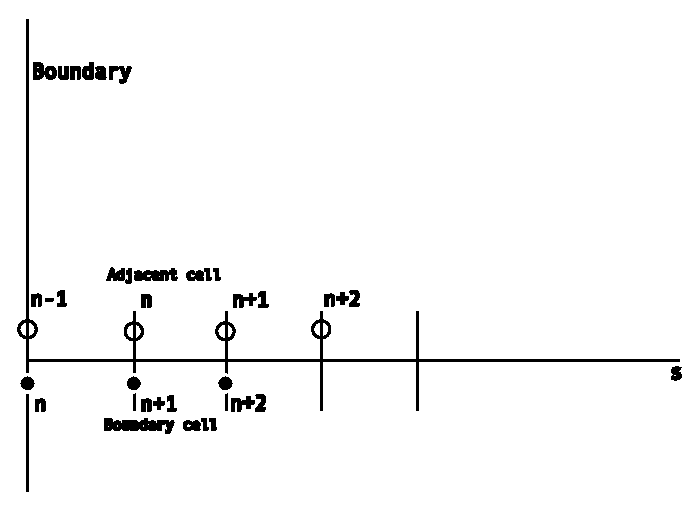
\includegraphics[width=0.5\textwidth]{Boundarydiff.eps}
\caption{Schematic showing the cells of intest in the differencing scheme when considering the boundary cell (Hollow circles) and the adjacent cell (Filled circles).  The figure shows the left hand boundary, for right hand simply reflect in the y direction}
\label{boundarydiffs}
\end{center}
\end{figure}

% Does new refer to zero-deriv and old to zero ?
\begin{figure}
\begin{center}
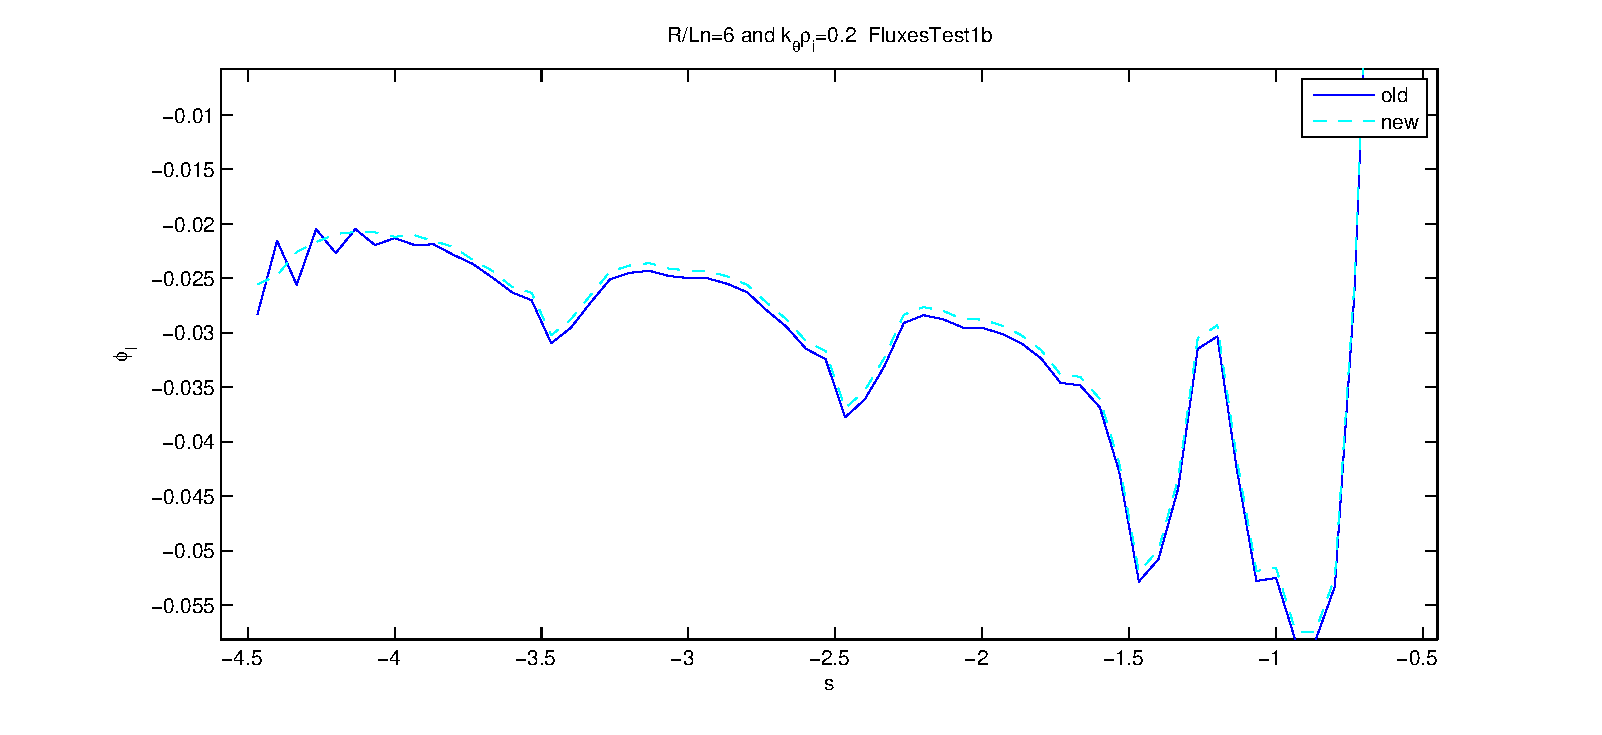
\includegraphics[width=0.5\textwidth]{fluxcomp.eps}
\caption{Figure showing the effect of the new open boundary conditions at the boundary. The new boundary has reduced cell to cell fluctuations giving a smoother solution.}
\label{fluxcomp}
\end{center}
\end{figure}

\noindent


The effect of the open boundary conditions is to remove the need for ghost cells in the differencing scheme while maintaining a high order scheme. It has reduced the amplitude of cell to cell fluctuations refelecting off the boundary (See figure \ref{fluxcomp}), which in turn, has reduced the need for adding artificial dissipation to the system to damp away these modes.  The dissipation, however, can not be wholly turned off in non-linear runs.  Note also that the dealiasing in nonlinear runs also has some dissipative effect in the perpendicular spatial directions.

\section{Parallel velocity grid - Trapping condition} %Added by Will 29/6/2008
(STILL EXPERIMENTAL AND UNDER DEVELOPMENT)
By contorting the velocity grid to conform to the electron trapping condition we are able to remove terms that involve derivatives in the parallel velocity direction.  This greatly speeds up linear run computation times but more significantly removes the need for numerical diffusion in the parallel velocity direction and lastly, provides resolution in the required areas.

This option is turned on by setting \name{vp\_trap} $= 1$ in the \name{CONTROL} namelist of the input deck.  A further parameter is needed in the \name{GRIDSIZE} namelist which is named \name{n\_trapped} which is the number of grid points within the trapped region of the velocity grid.

In the current implementation of the trapping condition, the number of cells in the s direction and the number of points in the parallel velocity direction add certain restrictions to the number of points that can be placed within the trapped region.

Firstly, for ease of differencing the bounce points of a specific $v_{\parallel 0}$ (The velocity on the low-field side) must occur exactly half way between two grid-cells, thus the number of grid cells in the s direction restrict both the number and initial values of $v_{\parallel}$.  The maximum number of bounce points available is given by \name{n\_s\_grid}$/2 - 1$.  The value of \name{n\_trapped} must be less than or equal to this.  If less is chosen then the code will select which points to use determined by the spacing between points (The closer to the boundary, the closer the bounce points become), the algorithm will iterate over the points, sequentially removing points until \name{n\_trapped} are left.  \name{n\_trapped} must also be less than \name{n\_vpar\_grid}.  Outside the trapping region the points are uniformly placed, the spacing is determined by the number \name{n\_vpar\_grid} $- 2\times$ \name{n\_trapped}.

\begin{figure}[h!]
\begin{center}
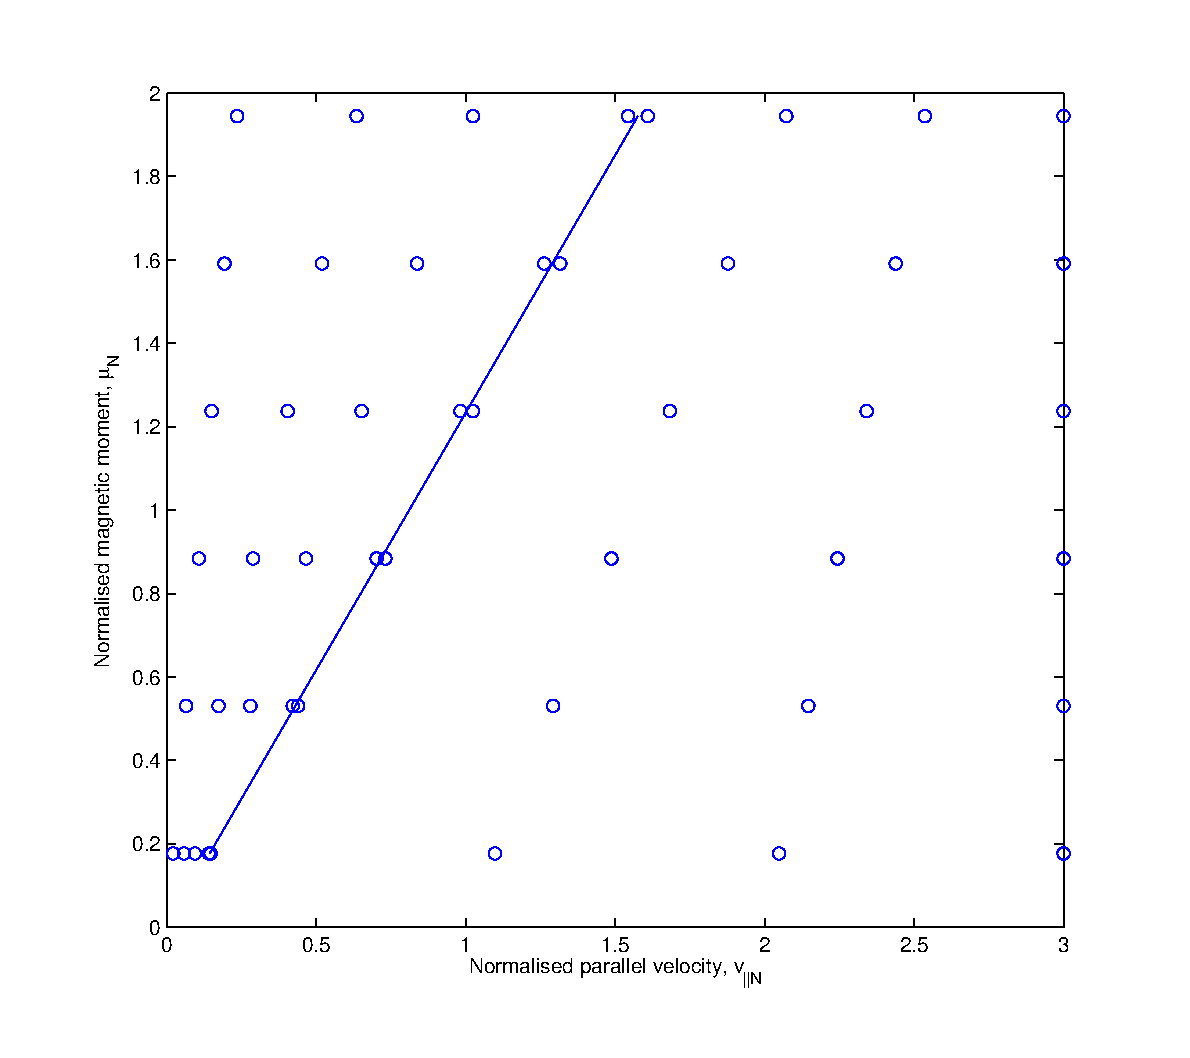
\includegraphics[width=0.4\textwidth]{traplowfield.eps}
\caption{Figure of parallel velocity grid points as given by the trapping condition, the line corresponds to the trapped/untrapped boundary $v_{||0} = \sqrt{2\mu(B_{max}-B_{min})+\cfen^{H}-\cfen^{L}}$.  In the above data, N_vpar_grid $= 16$ (only one half of the grid is shown as it is symmetric),n_trapped $= 4$ and $\mu = 6$. It must be noted that the total number of points within the trapped region (full grid) is $2\times$n_trapped.}
\label{lowfieldsidetrap}
\end{center}
\end{figure}

This algorithm gives the grid at the low field side (For an example see figure \ref{lowfieldsidetrap}), this is then propagated around the torus by the equation
\begin{equation}
v_{\parallel N} = \sqrt{v_{\parallel 0 N}^{2} + 2\mu_{N}(B - B_{0}) + \cfen- \cfen^{\rm L}}
\end{equation}
\noindent
where $B_{0}$ is the magnetic field at the low field side, and $\cfen^L$ is the centrifugal energy at the low field side.  When a bounce point is reached, the velocity becomes zero, and all velocity grid points after this along $s$ are set to zero and are ignored in the differencing.  The grid is also symmetric around $v_{\parallel}=0$.


Rules that must be followed, otherwise the code will throw you out,
\begin{itemize}
\item The value of \name{n\_trapped} must be less than \name{n\_vpar\_grid}/2
\item \name{n\_trapped} must also be less than or equal to \name{n\_s\_grid}/2$-1$
\item For optimal convergence $2\times$\name{n\_trapped} must be roughly half of \name{n\_vpar\_grid}. (This may no longer be true: See \issue{8} for latest updates on Gaussian integration (and section \ref{sec:gaussian-integration})
\end{itemize}

\section{Gaussian Integration}
\label{sec:gaussian-integration}

This is a short note on how the Gaussian integration is implemented in GKW. 

We wish to calculate the integral over the normalized parallel velocity $v_\parallel$ 
\begin{equation}
I = \int\nolimits_{v_{tp}}^{v_{pm}} g(v_\parallel) {\rm d} v_\parallel 
\end{equation} 
The integral is over (half of the) passing domain with the lower limit the trapped-passing 
boundary ($v_{tp}$) which is a function of $\mu$. We use Gaussian integration 
in combination with ${\rm vp\_trap = 1}$, in which case the parallel velocity grid must 
satisfy 
\begin{equation} 
v_{\parallel k}^2 = v_{\parallel 0}^2 + 2 \mu (B_0 - B_k) 
\end{equation} 
where $v_{\parallel k}$ is the parallel velocity at grid point k along the magnetic field, 
with $B_k$ being the local magnetic field, and the index 0 indicates the low field 
side position. We can therefore define only one set of parallel velocity gird points 
with the grid at different locations along the field line satisfying the equation 
above. The integral is therefore written in low field side coordinates 
\begin{equation} 
I = \int\nolimits_{v_{pt0}}^{v_{pm0}} g(v_\parallel ( v_{\parallel 0}) ) {{\rm d} v_\parallel \over 
{\rm d} v_{\parallel 0}} \biggr \vert_\mu \, {\rm d} v_{\parallel 0} 
\end{equation} 
From the relation between $v_\parallel$ and $v_{\parallel 0}$ it follows 
\begin{equation} 
{{\rm d} v_\parallel \over {\rm d} v_{\parallel 0}} \biggr \vert_\mu  = {v_{\parallel 0} \over 
v_\parallel } 
\end{equation}
We furthermore choose to write $g$ as 
\begin{equation}
{v_{\parallel 0} \over v_\parallel} g = \exp [-v_{\parallel 0}^2 ] z(v_{\parallel 0} )
\label{zdef} 
\end{equation} 
This choice is of course motivated by the expected dependence of $g$ on $v_\parallel$. The 
Maxwellian background will lead to the strong exponential decay. It is this exponential 
dependence that we would like to 'transform away' in order to obtain an efficient integration
algorithm. 

With the choices discussed above the integral is 
\begin{equation}
I = \int\nolimits_{v_{tp0}}^{v_{pm0}} \exp [ - v_{\parallel 0}^2 ] z(v_{\parallel 0}) {\rm d} v_{\parallel 0} 
\end{equation} 
Using the transformation 
\begin{equation} 
y = {\rm erf} (v_{\parallel 0}) \qquad {\rm with}\qquad {\rm erf}(v_{\parallel 0} ) = {2 \over \sqrt{\pi}} 
\int_0^{v_{\parallel 0}} \exp [-x^2] {\rm d} x
\end{equation} 
one obtains 
\begin{equation} 
I = {\sqrt\pi \over 2 } \int\nolimits_{ya}^{yb} z(y(v_{\parallel 0})) {\rm d} y 
\end{equation} 
with 
\begin{equation} 
ya = {\rm erf}(v_{tp0}) \qquad yb = {\rm erf}(v_{pm0} ) 
\end{equation} 
Finally, we transform the integral to the interval [-1,1], using the transformation 
\begin{equation} 
\alpha = {2 y \over yb - ya} - {ya + yb \over yb - ya} 
\end{equation} 
to obtain 
\begin{equation} 
I = {1\over 4} \sqrt\pi (yb - ya) \int_{-1}^1 z(\alpha(y)) {\rm d} \alpha 
\end{equation} 
The latter integral can then be solved by a standard Gauss Legendre integration using the points 
$\alpha_i$ and weights $w_i$ (which can be obtained from publicly available software) 
\begin{equation} 
\int_{-1}^1 z(\alpha(y)) {\rm d} \alpha = \sum\nolimits_{i = 1}^m  w_i z(\alpha_i) 
\end{equation} 

For the implementation we transform back to $v_{\parallel}$ 
\begin{equation} 
I = {1 \over 4} \sqrt\pi (yb-ya) \sum\nolimits_{i = 1}^m w_i \exp[ + v_{\parallel 0i}^2] {v_{\parallel 0 i} \over v_\parallel (v_{\parallel 0i} ) } 
g(v_\parallel(v_{\parallel 0i})) 
\end{equation} 
with the points of the grid $v_{\parallel 0 i}$ determined by the relation 
\begin{equation} 
{\rm erf}(v_{\parallel 0 i} ) = ya + (yb - ya)(\alpha_i + 1 )/2 
\end{equation}



\section{The collision operator}
\label{numerics:collisions}
The collision operator can be thought of as a convection/diffusion equation in velocity space and thus is differenced accordingly.
The velocity space boundary conditions are taken to be zero flux, which occurs naturally at the $\mu =0$ boundary and is artificially
imposed on the other three boundaries.  These boundary conditions guarantee the conservation of mass.  
Considering that the diffusion coefficient is velocity space dependent, and the grid can be non-uniform in the $\mu$-direction, the differencing scheme of the equations is chosen as follows for the parallel velocity direction
\begin{equation}
\frac{\partial}{\partial v_\parallel}\left(D\frac{\partial \hat{f}}{\partial v_{\parallel}}\right) \rightarrow
\frac{1}{v_{i+1/2\parallel}^{j}-v_{i-1/2\parallel}^{j}}\Big( D_{i+1/2}^{j}\left(\frac{f_{i+1}^{j}-f_{i}^{j}}{v_{i+1\parallel}^{j}-v_{i\parallel}^{j}}\right) - 
D_{i-1/2}^{j}\left(\frac{f_{i}^{j}-f_{i-1}^{j}}{v_{i\parallel}^{j}-v_{i-1\parallel}^{j}}\right)\Big),
\end{equation}
\noindent
where i denotes the point in the parallel velocity direction and j the $\mu$ direction.  When considering the cross-terms a four point 
interpolation method is used to calculate the half point values.  Four points are needed on a two-dimensional grid.
The friction term is differenced in the same way, but with a two point interpolation.  

To bypass the complications caused by non-uniform distribution of $\mu$ points (which in uniform in the $v_\perp$ coordinate), the code chooses the suitable version of the
collision operator that is uniform, and as such, can conserve mass (and parallel momentum) to machine accuracy.  

A further switch \textbf{selfcollcon} in the collisions input deck changes the momentum conservation from just the self-collisions for each species (selfcollcon = .true.) to absolute conservation (selfcollcon=.false, default=.true.). Note that the absolute conservation option is unphysical and only implemented for tests and benchmarks purposes.

\section{The Fourier representation} 

In a nonlinear run a rectangular grid of wave vectors ($k_\zeta,k_\psi$) is used. 
The nonlinearity is treated using fast Fourier transforms (FFT).
Different choices of FFT libraries are possible, but at present we use mostly the FFTW library \cite{FFT05}. 
For the nonlinear term a de-aliasing method is applied, i.e. the transformation to real space is constructed on a grid finer 
(number of grid points at least 3/2 larger in real space) than the Fourier modes represent. 
The de-aliasing method is non-conservative and has a dissipative effect on the finer grid scales, with the consequence that a 
numerical dissipation term in the spectral directions is generally not required.

Since the distribution function is a real quantity the number of
complex Fourier modes can be reduced by a factor two and a half plane
of wavevectors with $k_\zeta \ge 0$ is used.  Grid sizes in real space
are chosen so that they have only small prime factors. Such sizes lead
to particularly efficient computations with the standard FFT
libraries. There are no significantly more efficient grid sizes any
more, as it used to be in the past.

\section{Time integration}

GKW has several options for the explicit time integration: modified midpoint, fourth order Runga Kutta (recommended), 
and a second order scheme that is stable for hyperbolic equations. An implicit scheme is also implemented, but is still under development
and not yet recommended for general use (For latest updates see \issue{10}). 

\section{Poisson equation \label{Poisson-detail}}

The Poisson equation \ref{Poisson-adiabatic} is split into three linear terms which are stored in 
the main solution matrix,  but evaluated separately from the other linear terms. 
The calculation of the fields takes place in \File{fields.F90} subroutine \name{calculate_fields}.

The Poisson equation given in \ref{Poisson-adiabatic} can be rewritten.
\ifmoredetails
\begin{align}
  &\sum_{sp , ions }  Z_{sp} n_{R_0,sp} \biggl [ 
  2 \pi B \int {\rm d} v_{\parallel} {\rm d} \mu J_0(k_\perp\rho_{sp}) \hat g_{sp} + {Z_{sp} \over T_{Rsp}} [ \Gamma(b_{sp}) -1]\exp(-\cfennsp{sp}) \hat \phi 
  \biggr ] =  { n_{R_0,e}\exp(-\cfennsp{e})
    \over T_{Re}} ( \hat \phi - {\fsa{\hat \phi }}) \nonumber\\
  &
  \sum_{sp , ions }  Z_{sp} n_{R_0,sp} \biggl [ 
  2 \pi B \int {\rm d} v_{\parallel} {\rm d} \mu J_0(k_\perp\rho_{sp}) \hat g_{sp}
  \biggr ]
  + { n_{R_0,e}\exp(-\cfennsp{e}) \over T_{Re}} {\fsa{\hat \phi }} 
  = {} \nonumber\\
  &\qquad {} = 
  -\sum_{sp , ions }  Z_{sp} n_{R_0,sp} \biggl [ 
  {Z_{sp} \over T_{Rsp}} [ \Gamma(b_{sp}) -1]\exp(-\cfennsp{sp}) \hat \phi 
  \biggr ]
  + { n_{R_0,e}\exp(-\cfennsp{e}) \over T_{Re}} \hat \phi
 \nonumber\\
\end{align}
Solving for $\hat\phi$
\begin{align}
  &
  \sum_{sp , ions }  Z_{sp} n_{R_0,sp} \biggl [ 
  2 \pi B \int {\rm d} v_{\parallel} {\rm d} \mu J_0(k_\perp\rho_{sp}) \hat g_{sp}
  \biggr ]
  + { n_{R_0,e}\exp(-\cfennsp{e}) \over T_{Re}} {\fsa{ \hat\phi}} 
  = {} \nonumber\\
  &\qquad {} = 
  \left[-\sum_{sp , ions }  Z_{sp} n_{R_0,sp} \biggl [ 
  {Z_{sp} \over T_{Rsp}} [ \Gamma(b_{sp}) -1]\exp(-\cfennsp{sp})
  \biggr ]
  + { n_{R_0,e}\exp(-\cfennsp{e}) \over T_{Re}} \right] \hat \phi
 \nonumber\\
\end{align}
yields
\fi
\begin{align}
\hat{\phi }= -{1 \over A} \left[ \sum_{sp , ions }  \underbrace{Z_{sp} n_{R_0,sp} 2 \pi B \int {\rm d} v_{\parallel} {\rm d} \mu J_0(k_\perp\rho_{sp})}_{\name{poisson_int()}\rightarrow M^3} \hat g_{sp} + \underbrace{{n_{Re}\exp(-\cfennsp{e}) \over T_{Re}}
 \fsa{\hat\phi}}_{\name{poisson_zf()}\rightarrow \text{eq. \ref{eq:zonalmatrixform}}}
\right]
\label{eq:poisson2}
\end{align}
where the factor
\begin{equation}
 A =  \sum_{\rm sp, ions} n_{sp} Z_{sp} \left[ {Z_{sp} \over T_{Rsp}} ( \Gamma(b_{sp}) -1)\exp(-\cfennsp{sp}) - {\exp(-\cfennsp{e}) \over T_{Re} } \right] = M^4
\end{equation}
is evaluated in subroutine \name{poisson_dia}. The symbols $M^3$ and
$M^4$ number the matrices presented in this paragraph (and are not
``powers of $M$'' or so) and refer to sections of \name{mat}. In this
sense also $M^1$ and $M^2$ which contain the linear terms of the GKE
and are mentioned elsewhere denote sections 1 and 2 of the matrix
\name{mat}. The quantity $\fsa{\hat\phi}$ can be eliminated from
\ref{eq:poisson2} by taking the flux surface average of equation
\ref{eq:poisson2}.  
\ifmoredetails
\begin{align}
\fsa{\hat{\phi}} &= \fsa{-{1 \over A} \left[ 
    \sum_{sp , ions }  Z_{sp} n_{R_0,sp} 2 \pi B \int {\rm d} v_{\parallel} {\rm d} \mu J_0(k_\perp\rho_{sp}) \hat g_{sp} 
    + {n_{Re}\exp(-\cfennsp{e}) \over T_{e}} \fsa{\hat \phi}
  \right]} \nonumber\\
 &= \fsa{-{1 \over A} 
    \sum_{sp , ions }  Z_{sp} n_{R_0,sp} 2 \pi B \int {\rm d} v_{\parallel} {\rm d} \mu J_0(k_\perp\rho_{sp}) \hat g_{sp} 
    }
    + \fsa{-{1 \over A}{n_{Re}\exp(-\cfennsp{e}) \over T_{Re}} \fsa{\hat \phi}  
}
\end{align}
The expressions containing $\fsa{\hat\phi}$ are drawn together:
\begin{align}
\fsa{\hat\phi} - \frac{n_{Re}}{T_{Re}}\fsa{\frac{-\exp(-\cfennsp{e})}{A}} \fsa{\hat \phi}
  &= \fsa{-{1 \over A} 
    \sum_{sp , ions }  Z_{sp} n_{R_0,sp} 2 \pi B \int {\rm d} v_{\parallel} {\rm d} \mu J_0(k_\perp\rho_{sp}) \hat g_{sp} 
}\nonumber
\end{align}
\begin{align}
\fsa{\hat\phi}\left(
  1
  -
  \frac{n_{Re}}{T_{Re}}\fsa{\frac{-\exp(-\cfennsp{e})}{A}}\right)
  &=\nonumber\\
\frac{n_{Re}}{T_{Re}}\exp(-\cfennsp{e})\fsa{\hat\phi}\left(
  \frac{T_{Re}}{n_{Re}}\frac{1}{\exp(-\cfennsp{e})}
  -
  \fsa{\frac{-1}{A}}\right)
  &=
\end{align}
\fi
The zonal correction term can then be written as a function of the
distribution function, parameters and background quantities.
\begin{align}
{n_{Re}\exp(-\cfennsp{e}) \over T_{Re} } \fsa{\hat\phi}
&= { \fsa{
-{1 \over A} \sum_{sp, ions}  Z_{sp} n_{R_0,sp} 2 \pi B \int {\rm d} v_{\parallel} {\rm d} \mu J_0(k_\perp\rho_{sp})\hat g_{sp}
}
 \over
 {1 \over \exp(-\cfennsp{e})} \left({T_Re \over n_Re} + \fsa{{\exp(-\cfennsp{e}) \over A}}\right)} 
\label{eq:zonal}
\end{align}
The subroutine \name{poisson_zf} prepares matrices according to the definitions
\begin{align}
  Z &= -\frac{\ud s}{A} \\
  Y &= \frac{1}{\exp(-\cfennsp{e})} \left({T_Re \over n_Re} + \fsa{{\exp(-\cfennsp{e}) \over A}}\right)
\end{align}
which are used to express the right hand side of \ref{eq:zonal} in the form
\begin{align}
{n_{Re}\exp(-\cfennsp{e}) \over T_{Re} } \fsa{\hat\phi}
  &= {\sum_s Z M^3 {\hat g} \over Y}\ .
\label{eq:zonalmatrixform}
\end{align}
\ifmoredetails
Thanks to \ref{eq:zonal}, \ref{eq:poisson2} allows the subroutine
\name{calculate_fields} to calculate $\hat\phi$ explicitely.
\begin{align}
\hat{\phi } & = \sum_s Z M^3 {\hat g} + {\sum_s Z M^3 {\hat g} \over Y} \\
            & = {(Y + 1)\sum_s Z M^3 {\hat g} \over Y}\ .
\end{align}
\fi


To calculate $\hat\phi$ from the distribution function, first the integral
part \name{poisson_int} is evaluated using section $M^3$ of the
matrix.
\begin{equation}
a_i(k_y,k_x,s) = M^{3}_{ij} {\hat g}_j.
\end{equation}
Next, the zonal flow correction term, equation \ref{eq:zonal}, is evaluated
separately, using the special ``matrices'' $Z$ and $Y$.  First, the flux surface
average in the numerator is evaluated.
\begin{equation}
b_i(k_x) = \sum_s Z_{ij} a_j 
\end{equation}
Then each element is divided by the denominator from equation \ref{eq:zonal}.
\begin{equation}
c_i(0,k_x,s)) = b_i / Y_i(s) 
\end{equation}
The zonal correction term is then subtracted from the minuend in
equation \ref{eq:poisson2}.
\begin{equation}
d_i(k_y,,k_x,s)=a_i-c_i 
\end{equation}
Finally, all elements are divided by the factor $A$ ($A$ being identical
to $M^4$, the section 4 of ``the matrix of the linear terms'').
\begin{equation}
{\hat \phi}_i(k_y,k_x,s) = d_i / M^4_i
\end{equation}
The other linear terms are stored in sections 1 and 2 of the matrix and evaluated as 
$\hat{f_i}^\prime = \hat{f_i} + \delta t \cdot \hat{f_j} M^{1,2}_{ij}$ in \name{calculate_rhs}
after the evaluation of the fields.

\section{Notes on individual routines} 

This section discusses the individual routines and gives some details on the physics 
processes implemented. Here, not all the input and output or all the variables are 
discussed. It merely gives some details that should allow the reader to understand
the code better. 

\subsection{\src{linear_terms.f90}} %Added by Francis Jan 2008, not recently updated.
NOT INCLUDED here: centrifugal effects\\

In the treatment so far, the terms as implemented in the code were described in \ref{eqs:complete-set} as terms I-VIII. Here we link these terms to the routines in the code, as well as to \ref{Vlasov}, the Vlasov equation for the modified perturbation distribution function $g$.
\begin{equation} 
\label{1}
{\partial g \over \partial t} + (\underbrace{v_\parallel {\bf b}}_{I} + \underbrace{{\bf v}_D}_{II}) \cdot \nabla f + \underbrace{{\bf v}_\chi}_{III} \cdot \nabla g  
-\underbrace{{\mu B \over m}{{\bf B}\cdot \nabla B \over B^2}{\partial f \over \partial v_\parallel}}_{IV} = S. 
\end{equation}

Where the source from the Maxwellian background is given by eqn \ref{source}
\begin{equation} 
\label{2}
S =  - \underbrace{({\bf v}_\chi}_{V} + \underbrace{{\bf v}_D)}_{VI} \cdot \nabla_p F_M
-  {Ze \over T} \underbrace{[ v_\parallel {\bf b}}_{VII} + \underbrace{{\bf v}_D ]}_{VIII} \cdot \nabla \chi F_M  
\end{equation}

We also need the expansion of the drift velocity \ref{eq:drifts}
\begin{align}
\label{3}
{\bf v}_D &=& \underbrace{{1\over Ze} \biggl [ \underbrace{{m v_\parallel^2\over B}}_{1} + \underbrace{\mu}_{2} \biggr ] {{\bf B} \times \nabla B
\over B^2}}_{A} + \underbrace{{m v_\parallel^2 \over 2 Z e B} \beta^\prime {\bf b} \times \nabla \psi}_{3} 
 + \underbrace{{ 2 m v_\parallel \over Z e B } {\bf \Omega}_\perp}_{4} \cr 
\noalign{\vskip 0.2 truecm} 
&-& \underbrace{{m \Omega^2 R \over Z e B }  {\bf b} \times {\nabla R}}_{5}, 
\end{align}

In \src{linear_terms.f90} the various terms from these equations are input into the matrix in individual routines which will be described below.  Most of the computation in the code is done in the wave vector domain. All derivatives in the perpendicular direction are in Fourier space; but derivatives along the field line are done in real space (terms I and VII)

\par
Some routines in \src{linear_terms.f90} have two versions (identified by a postfix to the routine name), one for each of the second order and fourth order methods.  We concentrate here on the fourth order method since the other is out of order. The routines do the same thing with regards to which terms are implemented; the implementation is different for each method.  The linear terms all operate on the the distribution $g$ (often called $f$ in the code comments!), because the linear terms matrix is applied to \textbf{the array called \name{fdisi} which always contains $g$}. 

\par
\name{calc_linear_terms} is the master routine that calls the subroutines which put the terms I-XI (excluding term III) into the matrix.  Broadly, the first section puts the terms on the LHS of \ref{1}.  The second section calculates the source terms due to the maxwell background.\ref{2}.  The third section of \name{calc_linear_terms} calls the routines that input the field equations into the matrix. These are the equations that force the solution the be self consistent with the potentials calculated from the distribution function.  After each section is completed there is a call to \name {finish_matrix_section} in module \name {matdat} which stores the k index labels of the matrix for each section..

\par
Hence \name{calc_linear_terms} covers all the terms I-VII in \ref{eqs:complete-set} ( also labelled as the underbraced numbers in \ref{1}, \ref{2}, and \ref{3}), with the exception of term III, which is implemented in \src{non_linear_terms.f90}.

\subsubsection{\name{vpar_grad_df}, term I}
\name{vpar_grad_df} calculates the convection parallel to the field.  This routine also adds parallel velocity dissipation, which can be required for a numerically stable solution in nonlinear runs.
The dissipation is controlled by the input parameter \name{disp_par}.  This term is the free streaming motion along the field line, with derivative calculated in real space.

\subsubsection{\name{vdgradf}, term II}
\name{vdgradf} calculates the drift in the gradient of the eikonal term.

\subsubsection{\name{trapdf}, terms IV}
\name{trapdf} calcuates the mirror trapping terms dependent on the switch variable \name{trapping}.   This routine also adds perpendicular velocity dissipation, which can be required for a numerically stable solution in nonlinear runs. 
The dissipation is controlled by the input parameter \name{disp_vp}.

\subsubsection{\name{ve_grad_fm}, term V}
\name{ve_grad_fm} calculates the ${\bf E} \times {\bf B}$ drift due to the background distribution, as well as (optionally according to logical \name{nlapar}) the electromagnetic correction ${\bf v}_{\delta B_\perp}.$

\subsubsection{\name{neoclassical}, term VI}
\name{neoclassical} optionally includes the neoclassical terms according to the switch \name{neoclassics}.  Note many gyrokinetics codes disregard this term.

\subsubsection{\name{vpgrphi}, term VII}
\name{vpgrphi} calculates the landau damping term, dependent on the switch variable \name{landau}.  This is an acceleration along the field line with parallel derivative in real space.

\subsubsection{\name{vd_grad_phi_fm}, term VIII}
\name{vd_grad_phi_fm} calculates the  drift in the gradient of phi times the velocity derivative of the Maxwell background.  Note that Equation terms  \ref{3}.1 and \ref{3}.2 are combined as \ref{3}.A in the $E_D$.multiplier as defined in \ref{eqs:complete-set}.

\subsection{\src{non_linear_terms.F90}} %Added by Francis Feb 2008, needs checking again.

CHECK CONSISTENCY OF THIS SECTION

The Fourier amplitudes of the potential (and perturbed distribution function) are defined as 
\begin{equation} 
\phi_N(x) = \sum_k \phi_{Nk} \exp [ {\rm i} k x ] + c.c.  
\end{equation} 
Note that because the inverse discrete Fourier transform ($H_l$) is defined such that 
the values in real space ($h_n$) are given by  
\begin{equation} 
h_n = {1\over N} \sum_{l=0}^{N-1} H_l \exp [ {\rm i} 2\pi l n / N ] 
\end{equation} 
where $N$ is the total number of grid points of the discrete transform. The relation between the 
amplitudes and the discrete Fourier transform, therefore, is 
\begin{equation} 
H_l = N\phi_{Nk}
\end{equation} 
The wave vector $k$ is given by the standard relation  
\begin{equation} 
k = {2 \pi l \over N \Delta} 
\end{equation} 
where $\Delta$ is the grid distance. This relation is used to determine the size of the box 
in real space. It follows that the lowest non-zero wave vector $k_1$ determines $\Delta$ and
the size of the box $L = N\Delta$ 
\begin{equation} 
L = {2\pi \over k_1} 
\end{equation} 

\subsubsection{\name{add_non_linear_terms}, term III} 
\index{Non linear terms}
This routine implements the full term III with electromagnetic corrections.  Hence the routine finds the ${\bf E} \times {\bf B}$ drift of the perturbed distribution function, and adds the term:
\begin{equation} 
\label{Edrift}
{\bf v}_\chi \cdot \nabla g = {{\bf b} \times \nabla \hat{\langle \chi \rangle} \over B} \cdot \nabla g
\end{equation}
Without the elctromagnetic corrections, Term III of \ref{eqs:complete-set} becomes
\begin{equation}
{\rm III} = - {\bf v}_\phi \cdot \nabla g  \mathcal{T}\Big({\cal E}^{\psi \zeta}\left[\mathcal{T}^{-1}(ik_{\zeta} \hat{ \phi }) \mathcal{T}^{-1}(ik_{\psi} \hat g) -
\mathcal{T}^{-1}(ik_{\zeta} \hat g) \mathcal{T}^{-1}(ik_{\psi} \hat{ \phi })\right]\Big),
\end{equation}

where the expansion of the tensor sum uses the anti-symmetry of ${\cal E}^{\beta \alpha}$.  Note also that the diagonal elements of ${\cal E}^{\beta \alpha}$ are zero, and derivatives along $s$ are neglected. 

The gyroaveraged potential $\langle \phi_N \rangle$ is first calculated in the wavevector domain by multiplying the potential by the Bessel function $J_0$ (\ref {Bessel}). In k space the derivative of the potential is obtained by multiplying by $ik_\alpha$. 

Hence the implementation in the code is
\begin{equation}
a = i J_{0}(k_{\perp}\rho) k_{N,\zeta} \phi_{N,k} = ik_{\zeta}\rho_{\rm ref}{\langle \phi_{N,k} \rangle} 
\end{equation}
\begin{equation}
b = i J_{0}(k_{\perp}\rho) k_{N,\psi} \phi_{N,k} = ik_{\psi}\rho_{\rm ref}{\langle \phi_{N,k} \rangle} 
\end{equation}
Note the $\rho$ in the Bessel function is species dependent.  Also the normalization of the k vector $k = {k_N / \rho_{\rm ref}}$ introduces a multiplier of $\rho_{\rm ref}$
Hence the inverse Fourier transformation gives
\begin{equation}
ar = \mathcal{F}^{-1}(a) =  \rho_{\rm ref} {\partial {\langle \phi_N \rangle} \over \partial \zeta_{N}} = {\rho_{\rm ref} \over R_{\rm ref}} {\partial {\langle \phi_N \rangle} \over \partial \zeta} =  \rho_* {\partial {\langle \phi_N \rangle} \over \partial \zeta}
\end{equation}
\begin{equation}
br = \mathcal{F}^{-1}(b) =  \rho_* {\partial {\langle \phi_N \rangle} \over \partial \psi}
\end{equation}
%Incorrect, not all corrdinates are normalised the same.
Since the coordinates are normalised by $x_{\alpha,N} = {x_{\alpha} \slash R_{\rm ref}}$.  Here we have explicitly linked the normalizations of the k vector and coordinates to show that under the Fourier transform; $\rho_* {\partial \over \partial x_\alpha} \rightarrow {\rm i} k_\alpha$, as was intended in its definition. Put simply, a factor of $\rho_{*}$ appears after the inverse Fourier transform.

Similarly, the gradient of the distribution function in k space is found $a = i k_\psi g_{N,k}$, $b = i k_\zeta g_{N,k}$
and applying the inverse Fourier transform gives
\begin{equation}
cr = \mathcal{F}^{-1}(a) = \rho_* {\partial g_N \over \partial \psi}
\end{equation}
\begin{equation}
dr = \mathcal{F}^{-1}(b) = \rho_* {\partial g_N \over \partial \zeta}
\end{equation}

The tensor ${\cal E}^{\alpha \beta}$ (see \ref{efun}) is defined in \src{geom.f90} with name  {\name efun}. Note that although the tensor has two indices, each component varies along the field line due to the gradient in $B$. The array therfore has 3 indices with $efun{(i,2,1)}$ being the ${\cal E}(s)^{\zeta \psi}$ component. Calling this element of the array we now have all the components needed to calculate \ref{eq:nl-term}.  The factor of $\rho_*^2$ comes from the 2 inverse Fourier transforms.  Term III then appears in the code as
\begin{equation}
efun(i,2,1)*({ar*cr-br*dr})
\end{equation}

Finally this is Fourier transformed back to the wavevector domain and $\mathcal{F}({\bf v}_E \cdot \nabla g)$ is added to the RHS of the equations -  which were passed to the subroutine as an argument along with the distribution function when it was called from \src{exp_integration.F90}.

\par
The routine also calculates maximum velocities to be used in the timestep estimator.  The first time this routine is called it does some initialisations which are not repeated in later calls:  The sizes of the boxes in real space are calculated, the max k-vectors are calculated and the location of the $k_x = 0$ mode is determined.  Index arrays are also set up to relate the storage regime on the fast Fourier transform (fft) routine to the GKW storage regime. The remainder of the routine as described above is executed every time.

\section{The code}\label{thecode}

The package GKW consists of a README file (where a description of the full contents can be found),
Fortran 95 source files, various makefiles and related scripts, some documentation, some sample code input files,
some scripts associated with running and testing the code and tools to pre/post process data and perform visualisation.
This section describes what the code can do in terms of parallelisation and how it is structured
with respect to the solution of the equations presented in the previous sections. In order to do
this, we follow the various tasks the code performs as it runs and discuss the relevant modules to
that task. Instructions for building, installing and running the code can be found in section \ref{usage}.

Each source code file contains a module, except the main program file \src{gkw.f90}.
Each source file has either the extension \File{.f90} or \File{.F90}, the latter denoting the need to be pre-processed.
For the modules, each module name corresponds directly to the file name (which is always lower case), minus the suffix.
Therefore, in the following subsections, when referring to the module \name{GRID}, the corresponding source code can be found
in the file \src{grid.F90}.

The code does not come with any routines to perform FFTs, which are required for the computation of the non-linear term in Eq.~\ref{eq:nl-term}, and to transform some of the diagnostics into real space. No FFT's are required for a linear run and the code can be compiled without FFT functionality. The FFT's are presently performed via the external FFTW3 library \cite{FFT05}, for which the
\name{FFT} module provides an interface. Although more interfaces for various other portable Fortran FFT libraries could be
provided, the performance of the FFTW3 library has been found to exceed that of other alternatives significantly. In addition,
the FFTW3 library is fairly portable, so to date there has been no good reason to consider alternatives.

GKW is parallelised primarily using the Message Passing Interface (MPI)
\footnote{Shared memory parallelisation, implemented via OpenMP directives, is
now possible with the code and is documented in a later subsection}. Each
parallel process is responsible for solving the equations over a sub domain of
the space and a subset of the species. A process usually only has knowledge of
the part of the solution it is responsible for, unless explicitly communicated
between processes using the MPI library. The parallelisation is discussed in
more detail in a later section.

\subsection{Initialisation}

At the start of a run, the code will first call various basic MPI routines.
These give each process an individual rank (\name{processor_number}) and inform
each process of the total number of processors available for the computation
(\name{number_of_processors}). Checks are then performed to see if various
output or restart files are present. 

After this, the main input file is read. A single processor
is responsible for doing this. The input file contains several Fortran namelists, which
are described later. The first namelist is called \name{control} and is read in the module
\name{CONTROL}, and is responsible for controlling the basic switches for the physics, numerics and
some of the code output. Each module requiring input is responsible for reading its input
from this file. After each namelist is read, the processor that read the file broadcasts
the information to all the other processors via MPI. All processors can then individually
check that the input is allowed or satisfactory, and if necessary, abort the run.


\subsection{Parallelisation: local grid}

The sizes of the local and global grids and associated quantities are dealt with in
the module \name{GRID}. The namelist \name{gridsize} contains the input
variables for the grid sizes. The code can decompose the calculation over the
$s$, $v_\parallel$ and $\mu$ coordinates and the species. Given the number of
processors as input, the routines of \name{GRID} decide how the global solution
will be subdivided between the processors. Alternatively, a user can specify
explicitly the number of processors over which to subdivide the problem in each
divisible direction. 
%There are some restrictions for the case of collisions, and the Arakawa style differencing scheme. 
If a user explicitly sets 
an invalid combination, the code will abort at this point or earlier.
For the decomposition over the species or the $\mu$ grid, 1 point per processor is the minimum.
The minimum number of grid points per processor in the $s$ and $v_\parallel$ directions is limited to either 1 (when using the
second-order finite differences) or 2 (when using the fourth-order scheme). 
These minimum grid sizes dictate the maximum number of processors that can be used
in a given direction; the maximum is either the number of grid points in that direction (for the second-order scheme)
or half that value (for the fourth-order scheme). 
The parallelisation is discussed in more detail in Sect.~\ref{parallelisation}.

A processor is provided with various logical variables denoting if it is at a particular
boundary in the global domain together with the ranks of the processors that it
will need to communicate with (which are usually the ones responsible for adjacent
parts of the computational domain).

Once the local grid sizes have been confirmed, some MPI communicators are set up
to facilitate communication between processes responsible various subsets of
the whole domain. These are found in the \name{MPICOMMS} module.
They are particularly useful when performing a sum over a subset of the coordinates
when all the relevant points are not present on the local processor.

\subsection{Memory layout and allocation}
\label{memorylayout}
In GKW, the solution pertubation distribution
$g(k_\zeta,k_\psi,s,\mu,v_\parallel)$ for each species, together with the
various fields, are stored in the one-dimensional array \name{fdisi},
found in the module \name{DIST}. These quantities are defined at discrete grid
points, so can most conveniently be thought of as multidimensional arrays of
dimension 6 for the distribution function (three dimensions of space, two of
velocity, and one for the species) or 3 for the fields (three dimensions of
space). In the code we want to address them as multidimension arrays, via the
various grid indices, in order to perform initialisation and output
calculations. However, these arrays are embedded into the array \name{fdisi} in
order to facilitate the implementation of different types of numerical schemes
and optimisations.

The modules \name{DIST} and \name{INDEX_FUNCTION} are responsible for the tasks
of mapping the multidimensional arrays into \name{fdisi} and providing a means
to reference them. The \name{DIST} module is primarily responsible for deciding
where within \name{fdisi} those arrays should be stored (as a contiguous
block), and also making sure that each array is in a distinct part of
\name{fdisi}. The \name{INDEX_FUNCTION} module determines how the indices of the
multidimensional array are mapped to a single unique index for the one
dimensional array. This mapping can be
adjusted in order to improve parallel efficiency and (possibly) improve cache
efficiency. The default ordering is at present quite optimal, but manual
adjustments within the \name{INDEX_FUNCTION} module may yield further
improvement in some cases. These two modules are quite complicated and one
should look into those modules in the code.
% or at Sect.~\ref{appendix:fdisi} for a detailed explanation.
%FIXME Describe them somewhere?

The function which provides the array location within \name{fdisi} is
\name{indx()}.  This is used in many modules throughout the code, but
specifically {\it not} the time integration modules, which are designed not
to require it. As an example of how it is used, the value \name{phi} of the
potential at a radial grid point \name{ix}, a binormal grid point \name{imod}
and an $s$ grid point \name{i} is obtained in the code as
\begin{Verbatim}
  phi = fdisi(indx(iphi,imod,ix,i))
\end{Verbatim}
where \name{iphi} is an identifier for the potential.

In addition to the local solution $g$ and the various fields, the \name{fdisi_tmp}
array contains parts of the solution from other processors which have been
communicated via MPI datatypes. In the case of parallelising over the $s$-grid, the
fields are also decomposed, so parts of the potential from other processors
must also be present in order to calculate the derivative of
$\langle \phi \rangle$. The \name{indx()} function deals with referencing the
right part of \name{fdisi} so that other parts of the code do not need to make
special arrangements for processor boundary points.

The distribution function $f$ only ever exists temporarily in the array
\name{fdis_tmp}, and in diagnostics and elsewhere \textbf{a conversion from
$g$ to $f$ must be made (usually using the routine \name{get_f_from_g}, except
in optimised routines) when it is necessary to work with $f$}.

In general, each module is responsible for allocating any arrays they require.
The code attempts to do as much memory allocation as necessary early on, so
that if it will exceed the memory limits of a given machine, not much time will
have been wasted before the code aborts. When diagnostics are performed at the
end of a run, memory allocated for time integration is freed. 

%Something about cache efficiency in hybrid scheme?

\subsection{Linear terms}

The linear terms are calculated in the \name{LINEAR_TERMS} and \name{COLLISIONOP} module and put into a matrix which
is in \name{MATDAT}. The \name{LINEAR_TERMS} module is designed so that more new terms can be added by only
adding one new routine and calling it from within that module.

The linear terms all operate on the the distribution $g$ (often called $f$ in the code comments!), 
because the linear terms matrix is applied to \textbf{the array called \name{fdisi} which always contains $g$}.

\section{Code parallelisation}
\label{parallelisation}

At present, the parallelisation of the code is done primarily via decomposition
of the distribution function grid and the various species in a given run, using
MPI. There are now shared memory OpenMP directives implemented into the code
which enable more efficient parallelisation in some cases with a large number
of parallel processes. This is because performing parallel reduction operations
between a large number of processes becomes expensive; at some point, when
doubling the number of available processor cores, work sharing the local data
between 2 cores can become more efficient than doubling the number of MPI
processes.
The implementation and testing of the OpenMP parallelisation can be
found in Sec. \ref{sec:hybrid}. Here we describes the various
MPI parallelisation options and their potential consequences for code
performance. In the next section, a scaling test is shown for a Cray XT4.

\subsubsection{Simple parallelisation via the fields}

The equation for the distribution function
(without collisions) contains no derivatives in the magnetic moment $\mu$, which means that the distribution function for any
point in the $\mu$ grid can be updated independently of the other points in the $\mu$ grid. Similarly, the distribution
function for each species can be updated independently. Therefore, one can run up to
{\it number of grid points in mu} $\times$ {\it number of species} parallel processes (typically 32-64 processes) to update
the distribution function if parallelising over these two `directions'.
However, these points are coupled via the fields, which must be updated before the distribution
function can be calculated in an explicit time step. The field equations 
involve a summation over the whole of the velocity space and the species, for which the code requires
an inter-process reduction sum. In parallelising over these `trivial' directions, a process
can first perform a partial sum over local species and $\mu$-grid points, before participating in a sum
involving all the parallel processes. For each field, this sum must be performed at every point in the
3-dimensional space, and the result must be then known to every process. As the number of utilised processor cores increases, the
amount of data per core that is involved in the sum remains constant. How much the parallel efficiency of the code decreases
as the number of utilised processors is increased will depend on the algorithm used by MPI_ALLREDUCE and underlying system.
In this simple parallelisation case (and potentially in other cases) this ALLREDUCE operation is the bottleneck in parallel performance.

\subsubsection{Parallelisation over the $v_\parallel$ grid}

The equations have derivatives in parallel velocity, which in their numerical implementation involve points of the
distribution function along lines in the parallel velocity grid. The derivative at the local point requires at most
the value of the distribution function at 1 or 2 adjacent points (second or fourth-order scheme) in each direction along the parallel
velocity grid (see Sect~\ref{sec:finite-differences}). When decomposing the $v_\parallel$ grid, the calculation of a
$v_\parallel$ derivative at the end of a local grid will require 1 or 2 more points managed by another process.
These points need to be communicated from the
adjacent processor before the derivatives are performed. Typically, the 2 points at either end of the local parallel velocity
grid must be communicated to the corresponding adjacent process, and 2 points must be received from it.
Therefore, if we parallelise over the $v_\parallel$ grid we have this communication to perform in addition to that required
to calculate the fields as discussed in the previous subsection. On systems which support performing computation at the same
time as communication (such as a Cray XT4), this communication can be overlapped with the relatively
expensive nonlinear terms computation. However, in such a case we would still be left with the same field calculation
bottleneck as the number of processors responsible for the parallel velocity grid is increased. 

\subsubsection{Parallelisation over the $s$ grid}

In terms of the communication required for the derivatives along the $s$ direction, parallelisation over the $s$ grid is much
the same as for the $v_\parallel$ grid. However, splitting up the $s$ direction decomposes the space over which the fields
are calculated. This means that the ALLREDUCE operation for a given processor only needs to be performed between processors
responsible for the same part of the $s$ grid. If the number of processors over which the $s$ grid is decomposed is doubled,
then the data involved in the reduction sum is halved, and the number of processors that partake in the sum remains the same.
A consequence of this is that when parallelising only in the $s$ direction, no communication is needed to calculate
the fields. This is typically very favourable for parallel performance; one potential bottleneck would be effectively
removed (and the other can usually be overlapped with computation).

\subsubsection{Parallelisation over the $\mu$ (and $v_\parallel$) grid with collisions}

If the collision operator is used, the parallelisation over the $\mu$ grid is not simply via the fields as derivatives are
present. The second-order local derivative for the collision operator uses all the adjacent points in the velocity space
(see Sect. \ref{numerics:collisions}). Although only 1 point must be exchanged between adjacent processors, any 1 processor
may need to perform this exchange between 8 processors. If parallelising over the $v_\parallel$ and $\mu$ grids at the same time, this would mean
communication between 6 additional processors (when the grid is decomposed over more than 2 processors in each direction) when compared to a run without
collisions. Ideally we would like to avoid parallelising over both the $v_\parallel$ and $\mu$ grids till other options have been exhausted.
Parallelising over the $v_\parallel$ grid, but not the $\mu$ grid should be equally expensive with or without collisions, since there is no difference
in the grid points communicated. Parallelising instead over just the $\mu$ grid, but not the $v_\parallel$ grid would be more expensive with collisions than without, although typically cheaper (when using the default
fourth-order finite-differences) than the previous case using only $v_\parallel$.

\section{Parallel performance (pure MPI), Cray XT4 \label{scaling-orig}}

\begin{figure}[h] 
\begin{center}
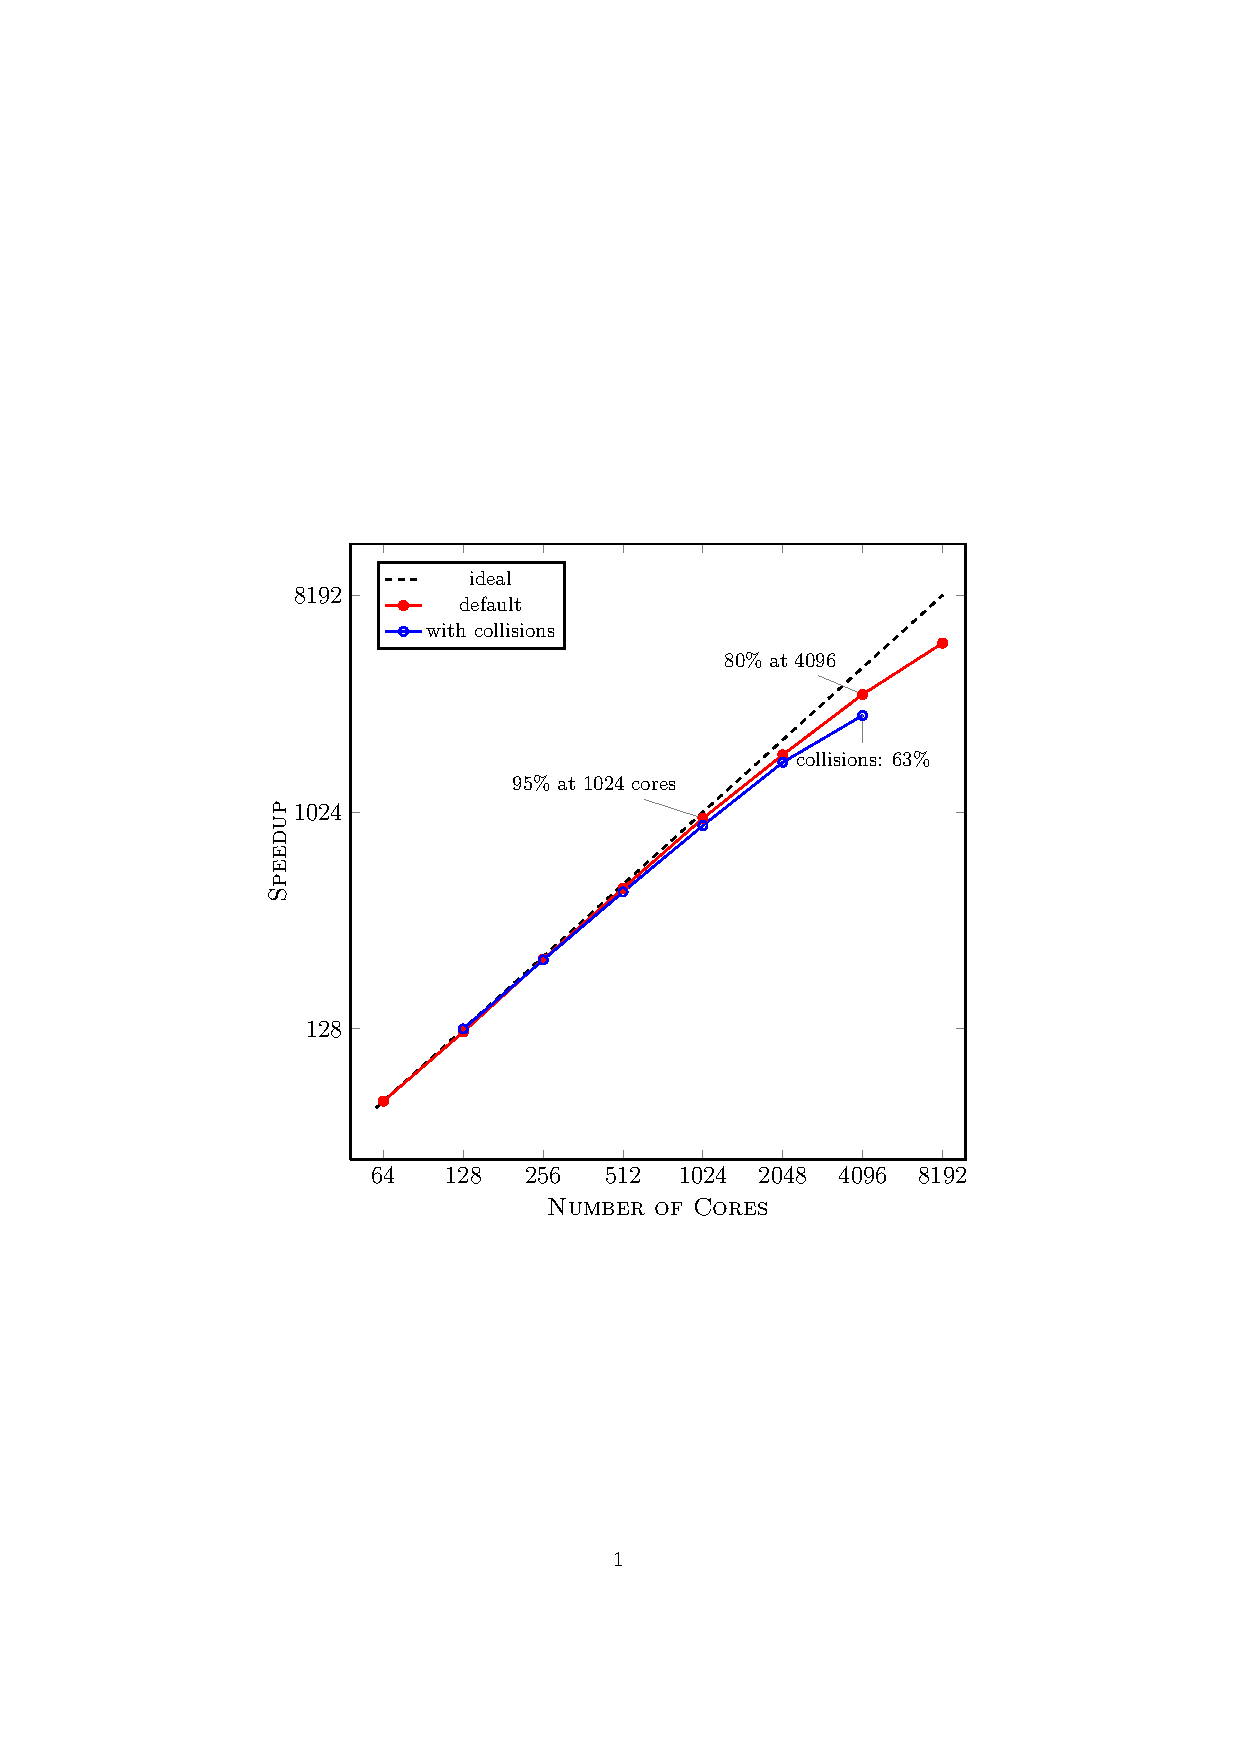
\includegraphics[width=0.5\textwidth,clip]{performance}
\caption{
  Parallel performance for a typical sized problem on HECToR (Cray XT4), both without and 
  with the collision operator turned on. Due to machine memory constraints, this problem can run with
  a minimum of 64 cores without collisions and 128 cores with. The performance/speedup is based on the
  time taken to perform the main time integration loop of the code and is scaled such that it is equal
  to the number of cores when the smallest possible number of cores is used. The parallel efficiency,
  based on $100$\% for the smallest number of cores, is noted at several points on the plot.
}
\label{scaling}
\end{center}
\end{figure}
Here we make a simple assessment of the parallel performance of the code on a Cray XT4 (HECTOR). We define the performance
as the amount of main time loop computation done by the code per unit time. In the ideal case, a doubling in the
number of processor cores used will double the amount of computation done per unit time (or halve the time required
to do a fixed number of time steps).
We consider a non linear problem of fairly typical size that we believe to be reasonably well converged with respect to grid
resolution. As mentioned in Sect.~\ref{memorylayout}, we can change the data memory layout to potentially
tweak the parallelisation and cache efficiency of the code. We have experienced some variation in performance due to these
adjustments. However, we do not yet have enough experience of how to optimally prescribe the layout depending on grid size and parallelisation options,
so for the purpose of this test, we keep the layout fixed to the default. We perform a test with a resolution of 83 radial wave vectors, 21 bi-normal modes, 4 species, 16 $s$ grid points, 16 $\mu$ grid points and 64 $v_\parallel$ grid
points, using fourth-order finite-differences in double precision. Two cases are considered, one using the collision operator and one
without. Due to the memory available per processor core, a minimum of 64 processors are required for the former case and 128 for the latter. 
Using a second-order finite-difference scheme and/or a single precision calculation can reduce this minimum. From the parallel algorithm
perspective, the upper limit on the number of parallel processes used for this case is 16384. Using second-order finite differences would increase this maximum to 65536 cores.
However, only up to 8192 cores were available on the hardware at the time of testing.

Before deciding how to producing a scaling plot for this testcase (such as in Fig.~\ref{scaling}), some preliminary investigations on
the effects of parallelising in each direction were made. Using the `trivial' directions alone, the test case parallelises over the minimum
64 processors for the default case. The difference in performance
between this parallelisation and parallelising primarily over the parallel velocity grid is fairly small, the `trivial' directions giving
less than $10$\% better performance than with the $v_\parallel$ direction. Parallelising primarily over the $s$ grid at
64 cores (using the maximum number of cores in the $s$ direction before using the simple direction) yields a performance which is almost identical
to that using only the `trivial' directions. It seems that for 64 processors, the communication needed for the derivatives has little (if any) effect
on the parallel performance. To get an idea of the relative expense of parallelising over $s$ and $v_\parallel$, two tests were made by starting with 64
cores (using only the trivial parallelisations), then varying either the number of processors in the $v_\parallel$ direction
or the $s$ direction until a total of 512 cores were used. The reduction in efficiency with increasing processors was greater with $v_\parallel$, with the $s$
parallelisation performing around $6\%$ better at 512 cores (at $>95\%$ of the efficiency at 64 processors).

A scaling test was performed for the collisionless case up to 8192 cores. Fig.~\ref{scaling} shows how the performance increases with the number of cores.
For the first point at 64 cores, only the `trivial' directions are used for the parallelisation, since that combination provides the best performance 
(but only by around $1\%$). Since the $s$ direction is the preferred parallelisation direction (least expensive in terms of performance), the number of 
processors in $s$ doubled between each point on the graph up to 512 cores, where the maximum of 8 processors in $s$ is used. Beyond that point, the more expensive $v_\parallel$ grid is decomposed until
8192 cores are used. At 8192 cores, the code runs at $63\%$ of the efficiency at 64 cores.

Following the discussion in the previous subsections, we should expect that with collisions, parallelisation over the $\mu$ direction
is more expensive than over the $s$ direction. Therefore, the scaling test for collisions (as shown in Fig.~\ref{scaling}) starts at 128 processors fully parallelised over the $s$ direction
and over the species, using only 4 processors in $\mu$. Then, the number of processors in $\mu$ is doubled, until 512 cores are used. At 1024 cores, it is cheaper to use 32
processors in $v_\parallel$ and only $1$ in $\mu$, since this avoids using parallelisation in both those directions together. For the final 2 points on the graph, the 
number of processors in the $v_\parallel$ and $\mu$ are either identical, or there are twice as many in $v_\parallel$. Since these
parallelisation combinations give the best performance (considerably better than using the same ones as without collisions), careful consideration should be given to
the number of processors used in each direction when using collisions. At 4096 cores the efficiency is $63\%$ of that at 64 cores.

In both cases considered we see decreasing performance gains when we begin to parallelise in
less favourable directions. Running the tests in single precision would mean less data communicated, so may improve
scaling (but at the same time would likely reduce the time between communication, or the time available for overlapping communication with computation). Running with the second
order finite difference scheme would allow double the number of cores in the $s$ direction and may improve the efficiency
at a large number of cores. If different test cases are considered, it may well be that more resolution in a particular direction
is needed, which would then lend itself to further scaling.

% Something about cartesian topology ordering
For hardware in which not all processor interconnects are equal in speed, the ordering of the MPI communicators within the cartesian topology 
can have a significant effect on parallel performance.  Current high performance machines appear with multiple shared memory cores on interconnected nodes are one example.  Given the above discussion of the bottleneck in global reduction operations, it is preferable that the $s$ direction decomposition should be over the slowest communication direction.  The GKW default setup assumes that MPI rank ordering is done with adjacent physical processors adjacent in the rank ordering.  Testing of a collisionless case on a Cray XT6 (HECTOR phase-2b with 24 cores per node) with 1344 cores indicated that the default dimension ordering (Species, $\mu$, $v_\parallel$, $s$) was optimal.  The configuration ($v_\parallel$, Species, $\mu$, $s$), was 30\% slower, even with exact multiples of the $v_\parallel$ grid (presumably) on a single node.  This is counter-intuitive, since one would expect putting the $v_\parallel$ direction first to be optimal. Configurations with $s$ first were up to 80\% slower. The ordering can be simply reconfigured near the top of \File{grid.F90}.  The optimal configuration will depend on hardware and problem size, and conducting tests prior to expensive runs is recommended.


\section{Parallel performance (hybrid, MPI+OpenMP), BlueGene/P \label{sec:bluegene}}
The performance of pure MPI parallelisation has also been compared to hybrid parallelisation MPI+OpenMP (see Sec.~\ref{sec:hybrid} for details on the hybrid scheme) for a typical non-linear electromagnetic case with kinetic electrons. The problem size is almost the same as in the previous section: 83 radial wave vectors, 20 bi-normal modes, 4 species, 32 $s$ grid points, 8 $\mu$ grid points and 64 $v_\parallel$ grid. A case without collisions and a case with collisions ($R_\textrm{ref}=3$, $T_\textrm{2}$ and $n_\textrm{ref}=6$, was investigated.  In contrast to the previous section, the full collision operator \textit{with} mass and momentum conservation was used\footnote{How much the scaling is affected by the communication required for the momentum conservation has not yet been fully investigated by comparisons on the same machine. Limited tests on BABEL indicated that momentum conservation caused a consistent 4\% slowdown up to 4096 cores, but it could become more (or less) important at higher number of cores (note that it is overlapped with derivatives communications when the MPI implementation supports this).  The version of GKW tested on BABEL did not yet have OpenMP implemented in the calculation of the momentum conserving field. Comparison of timings for the regular fields indicate that implementing this would give a 4\% (2\%) speedup at 4 (2) threads without MPI, but with MPI it will likely make no difference if the scaling bottleneck is in the overlapped derivatives communication.}.

The tests were conducted on the BlueGene/P BABEL (4 cores at 850MHz and 2GB of memory per node \url{http://www.idris.fr/eng/User_Support/bg_support.html}) for which the number of OpenMP threads per node can be 1, 2 or 4. The executable was compiled from revision 2076 of GKW source with O4 optimisation level (typically $10\%$ faster that O2/O3 optimisation for a compilation without OpenMP and $5\%$ faster for a compilation with OpenMP) and double precision. Due to the small amount of memory per node available on BABEL at least 512 cores were required to run the problem under consideration (to be accurate, the run fits on 256 cores but the execution is then very slow). For all the runs in this section, the number of MPI processes in the species and $s$ direction was \name{n_procs_sp}=4 and \name{n_procs_s}=16, respectively. The number of processes in the $\mu$ direction was \name{n_procs_mu}=8 for the collisionless case and \name{n_procs_mu}=4 for the case with collisions (except when 4 threads were used at 512 cores where \name{n_procs_mu} was reduced to 4 and 2, respectively). This means that the MPI parallelisation over the three most favorable directions was maximised to start with and the scaling of the least favorable direction, $v_\parallel$, was then compared to the OpenMP scaling by increasing either \name{n_procs_vpar} or the number of threads per node. For instance, a collisonless run on 2048 cores was performed on 1 thread with \name{n_procs_vpar}=4 or on 2 threads with \name{n_procs_vpar}=2.  The tests were conducted with a typical set of diagnostics with NAVERAGE=100, and with the nonlinear timestep estimator on, both were found to have little effect on the scaling performance (for the single threaded case at least).

The results of the tests are summarised in Table~\ref{table:nocol} (no collisions) and Table~\ref{table:col} (with collisions). The corresponding speed-up and total main loop time is displayed in Fig.~\ref{scalingBABEL} and \ref{scalingBABEL:total}, respectively. Hybrid parallelism with 4 threads is especially useful with collisions and allows to recover the scaling obtained without collisions near the MPI limits. 
\begin{table}
\begin{center}
\begin{tabular}{|c|c|c|c|c|c|c|}
\hline
cores & 512 & 1024 & 2048 & 4096 & 8192 & 16384\\
\hline
1 thread - no OMP& 203.5h & 212.8h & 227.9h& 255.3h & 304.3h & 408.4h \\
(time, efficiency) & 100\% & 95.6\%  & 89.3\%  & 79.7\%&66.9\% & 49.8\%\\
\hline
1 thread & 214.4h & 222.1h & 237.0h& 263.6h & 316.6h & 551.0h \\
(time, efficiency) & 100\% & 96.5\%  & 90.5\%  & 81.3\%& 67.7\% & 38.9\%\\
\hline
2 threads &221.1h & 225.5h & 233.3h& 255.1h & 313.2h & 493.1h \\
(time, efficiency) & 100\% & 98.0\%  & 94.8\%  & 86.7\% & 70.6\% & 44.8\%\\
\hline
\end{tabular}
\caption{Case without collisions. Total main loop time (in hours) for 600 time steps and strong scaling efficiency based on the case with 512 cores.}
\label{table:nocol}
\end{center}
\end{table}
Compilation without OpenMP is slightly faster (due to different cache efficiencies in the matrix ordering). This was also observed on HECTOR. (This has since been changed, both now use the same sort ordering so there is no longer any cache penalty for openmp)
\begin{small}
\begin{table}
\begin{center}
\begin{tabular}{|c|c|c|c|c|c|c|}
\hline
cores & 512 & 1024 & 2048 & 4096 & 8192 & 16384\\
\hline
1 thread& - & 290.0h & 317.9h & 373.1h & 519.2h & - \\
(time, efficiency) & (100\%) & (92.6\%)  & (84.4\%)  & (71.9\%)& (51.7\%) & - \\
\hline
2 threads & 268.4h & 283.0h & 300.4h& 323.4h & 480.6h & 713.6h \\
(time, efficiency) & 100\% & 94.8\%  & 89.4\%  & 83.0\%& 55.9\% & 37.6\%\\
\hline
4 threads & 281.7h & 283.5h & 294.9h & 314.6h & 380.5h & 506.1h \\
(time, efficiency) & 100\% & 99.4\%  & 95.5\%  & 89.5\% & 74.0\% & 55.7\%\\
\hline
\end{tabular}
\caption{Case with collisions (including momentum conservation). Total main loop time (in hours) for 600 time steps and strong scaling efficiency based on the case with 512 cores. On 1 thread, the run at 512 cores was out of memory and the strong scaling efficiency was calculated using the results on 2 threads. }
\label{table:col}
\end{center}
\end{table}
\end{small}

\begin{figure}
\begin{center}
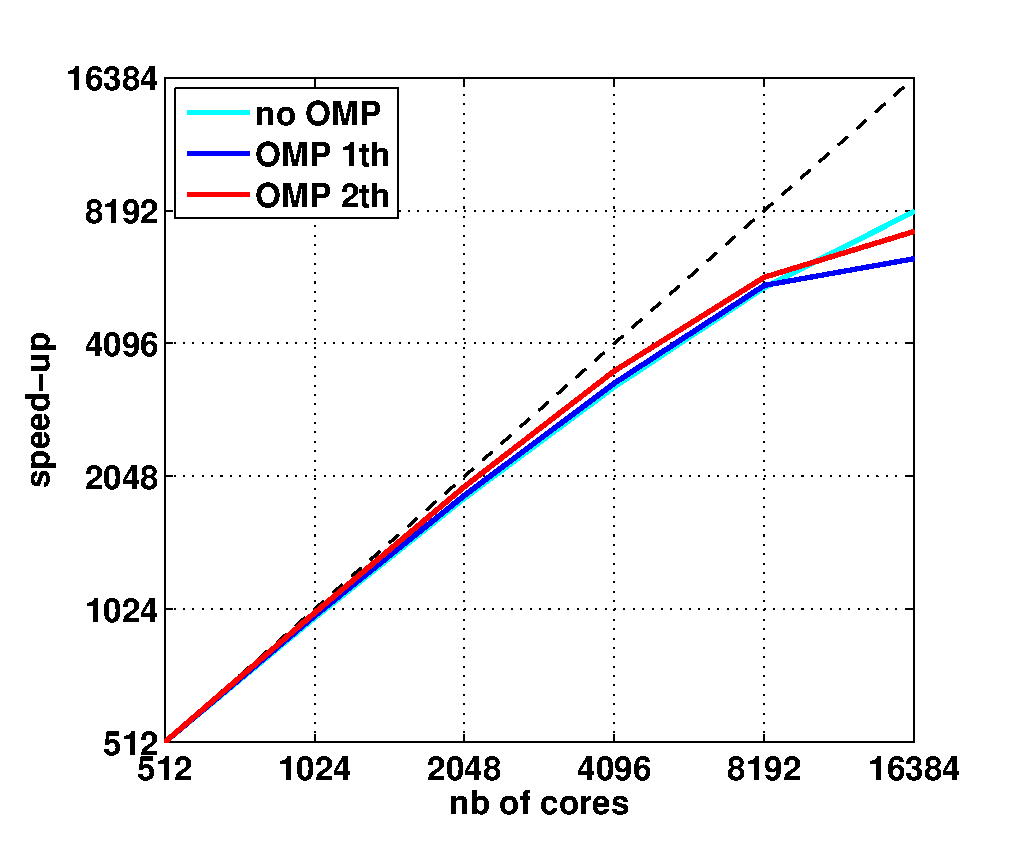
\includegraphics[width=0.4\textwidth]{speedupnocollisions.eps}%
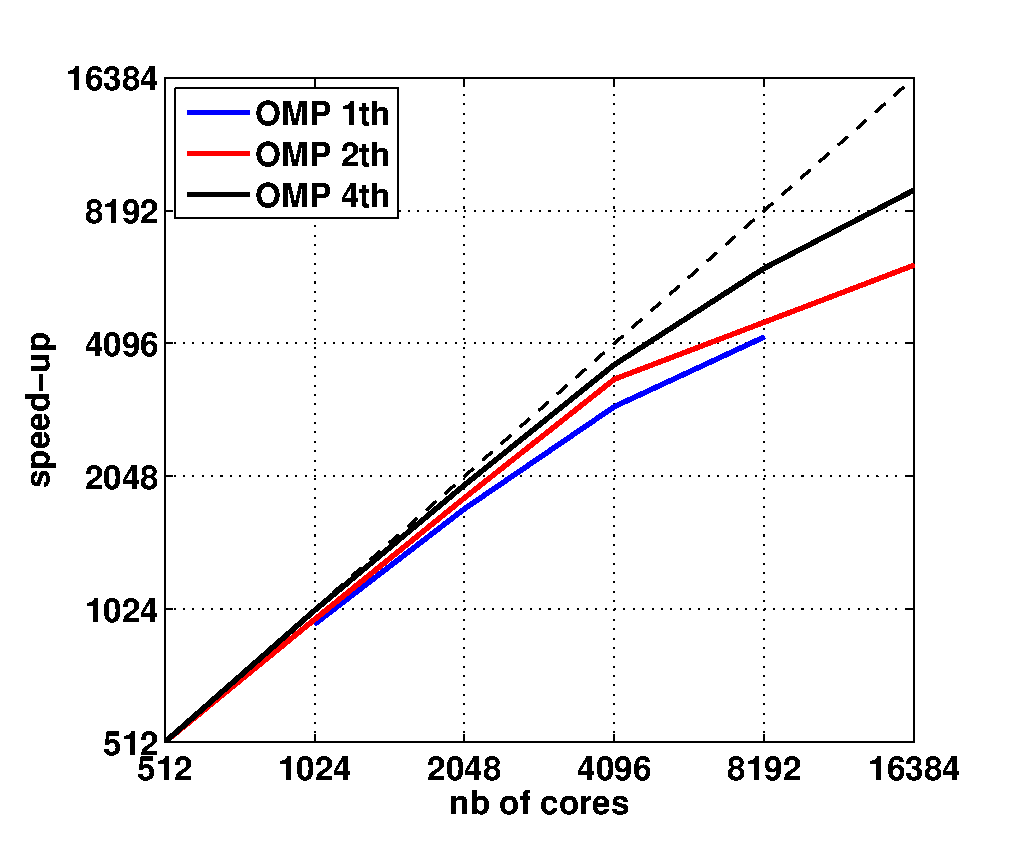
\includegraphics[width=0.4\textwidth]{speedupcollisions.eps}
\caption{ Parallel performance for a typical sized problem on BABEL (BlueGene/P), both without (left plot) and 
  with (right plot) the collision operator (with momentum conservation) turned on. The performance/speedup is based on the
  time taken to perform the main time integration loop of the code and is scaled such that it is equal
  to the number of cores when the smallest possible number of cores is used.}
\label{scalingBABEL}
\end{center}
\end{figure}
\begin{figure}
\begin{center}
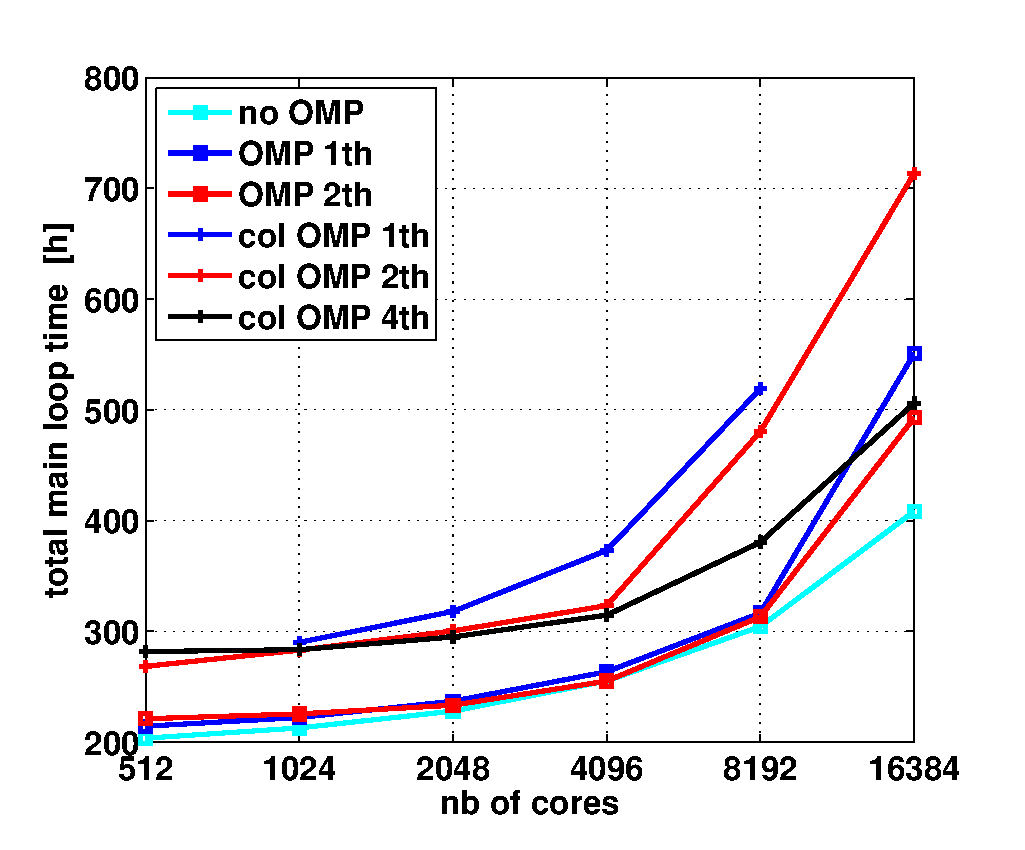
\includegraphics[width=0.5\textwidth]{totaltime.eps}
\caption{ Total main loop time in hours for the cases studied in this section.}
\label{scalingBABEL:total}
\end{center}
\end{figure}

A test has also been performed with the number of modes increased to NX=183 and NMOD=32 with the results summarised in Table~\ref{table:bigcol}.
\begin{small}
\begin{table}
\begin{center}
\begin{tabular}{|c|c|c|c|c|}
\hline
cores & 2048 & 4096 & 8192 & 16384\\
\hline
1 thread& 1166.4h & 1369.1h & 1731.7 h & - \\
(time, efficiency) & 100\% & 85.2\%  & 67.4\%  & -\\
\hline
2 threads & 1094.9h& 1164.4h & 1412.5h & 2317.3h \\
(time, efficiency) & 100\% & 94.0\%& 77.5\% & 47.3\%\\
\hline
4 threads &1081.7h & 1136.5h & 1305.4h & 1692.5h \\
(time, efficiency) & 100\% & 95.2\% & 82.9\% & 63.9\%\\
\hline
\end{tabular}
\caption{Case with collisions (with momentum conservation), NX=167 and NMOD=32. Total main loop time (in hours) for 600 time steps and strong scaling efficiency based on the case with 2048 cores. }
\label{table:bigcol}
\end{center}
\end{table}
\end{small}

\pagebreak


\section{Parallel nonspectral performance (pure MPI), Helios}

The nonspectral version of the code additionally parallelizes over the radial (x) direction (with the exception an implicit solve for the polarization term).  The nonspectral 
version of the code spends proportionally more time in the fields calculations than the spectral version, since the multi-point averages use for the gyroaverages are much slower 
than the Bessel functions of the spectral version. (The nonlinear terms, by contrast, are much faster since they only require 1D FFTs.)

Since the ``diagonal part'' of the fields solve is only 3 dimensional, it cannot parallelise over the velocity space or species.   This is true in both the spectral and nonspectral
versions, but in the spectral version, the diagonal part of the fields solve takes a neglible of CPU time.  To allow efficient scaling for the nonspectral version, the fields solve 
work is additionally parallelised over the toroidal modes using the same communicators that are elsewhere used to distribute work over the velocity space and species. 
This feature also reduces the fraction of time spent in the implicit polarization solve, which is radially global. Two allgather communications are therefore required in the fields
solve: The first in x before the polarization solve, and the second in nmod after the polarization solve so that every processor obtains the result for every toroidal mode. 
Since these are both gather operations of 3d quantities, they are relatively fast compared to the reductions and communications of ghost cells.  

Parallelization over the x direction brings the same benefits for reducing the reduction operations in the field solve as the parallelism over the s direction. The additional
penalties of extra ghost cell and allgather communications in the fields solve are outweighed by the benefit that this brings.  The result is that parallelism over x is always more
efficient than parallelism over parallel velocity (which in the nonspectral case performs much worse than in the spectral case due to the larger fraction of time in the field
solve).  For more details see \raw{doc/GKW_MPI_nonspectral.pdf}.

Scaling tests of the radially nonspectral version of the code (Fig. \ref{scalingHelios}) were performed on the Bull IFERC Helios machine (Intel Sandy Bridge with fat tree topology Infiniband
communication network).  As with the scaling test described in Sec. \ref{scaling-orig}, the `trivial' parallel directions were used first, followed by s, then x (although not to maximum), then finally vpar.
Two cases were chosen to represent a medium and a large physics case simulation, with gridsizes
\begin{verbatim}
NX = 256, N_s_grid = 32,  N_mu_grid = 16,  N_vpar_grid = 32,  NMOD = 16, number_of_species = 2
\end{verbatim}
for the medium case, and 
\begin{verbatim}
NX = 512, N_s_grid = 64,  N_mu_grid = 16,  N_vpar_grid = 64,  NMOD = 43, number_of_species = 2
\end{verbatim}
for the large case.

The radial box size was \texttt{lx = 128} or \texttt{lx = 256} respectively, which resulted in 6 x ghost points required for the gyroaverages (only two are communicated for the derivatives).  Since the number of ghost points must be less than the number of local points, this sets the maximum limit of \texttt{n_procs_x = 32} or \texttt{64} repsectively.

\begin{figure}[htb!]
\begin{center}
\includegraphics[width=0.48\textwidth]{scaling-helios-med3}
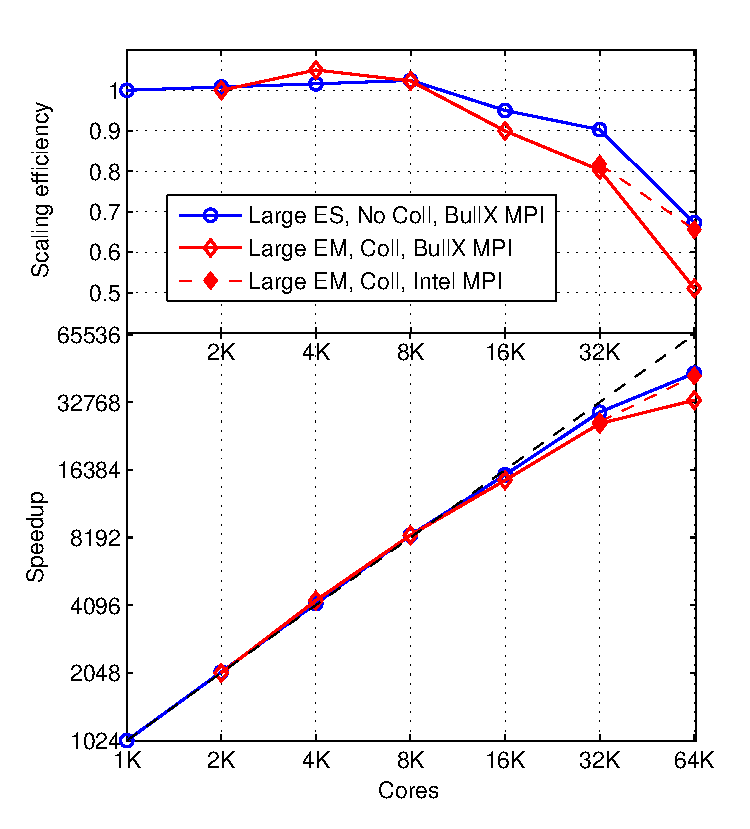
\includegraphics[width=0.49\textwidth]{scaling-helios-large3}
\caption{ Strong scaling performance for the medium and large sized nonspectral problems on Helios. 
          The speedup is based on the time taken to perform the main time integration loop 
          of the code and is scaled such that it is equal to the number of cores when the smallest possible number of cores is used.
          BullX MPI seems to perform better at ghost cell communications of derived datatypes while Intel MPI seems to perform better at the large
collective operations.  Which is better therefore depends on which MPI communication is dominant for a given problem.}  
\label{scalingHelios}
\end{center}
\end{figure}

For the medium problem size, the maximum possible \texttt{n_procs_x=32, n_procs_vpar=16} would allow a theoretical maximum of 131,072 cores (65,536 with collisions).  For the large problem size, the maximum possible \texttt{n_procs_x=64, n_procs_vpar=32} allows a theortical maximum of 1,048,576 cores (524,288 with collisions).  These results compare favorably with the spectral scaling tests: 
The parallelism over x removes any scaling performance penalty associated with the use of the collision operator
(which adds 20\% to all runtimes).  



% related to auctex mode and latex-preview-mode in Emacs:
%%% Local Variables:
%%% mode: latex
%%% TeX-master: "doc"
%%% End:

\chapter{Obtaining, building and running the code} \label{usage}

\section{Getting the code}

To obtain the latest version of the code (which should approximately
correspond to the latest version of this documentation), you should use the
git revision control system (\href{http://git-scm.com/.}
{http://git-scm.com/.}). The git program is installed on many
systems as the \name{git} command. Assuming you are using \name{git}, you can
check out the code with the command
%git clone http://gkw@bitbucket.org/gkw/gkw.git gkw-read-only
\begin{verbatim}
  git clone git@bitbucket.org:gkw/gkw.git gkw
\end{verbatim}
To push changes, you will need a bitbucket account to be given write permissions.

% Not yet sure how this will be relvant to bitbucket:
%[Some advice on which tagged versions to use, or how to download without git.]%

% This clone does not allow changes to be written back to the repository.
% Instructions for developers with commit permissions 
% can be found at \href{http://code.google.com/p/gkw/source/checkout}{
% http://code.google.com/p/gkw/source/checkout}.

% Alternatively, a reasonably stable version of the code can be obtained as a
% tarball from the downloads section
% (\href{http://code.google.com/p/gkw/downloads/list}
% {http://code.google.com/p/gkw/downloads/list}).
% At present, the version of the code found there is based on the CPC release
% (associated with the CPC paper \cite{CPC-paper}). The tarball is not often
% updated and will not have the latest code features. 

\section{Building the source code}

% If using a version obtained in a tarball, it is suggested to look at the
% \File{README} file found within for specific compiling instructions. The
% guidance of the following sections pertains primarily to the latest version of
% the code obtained via Subversion.

There are two methods provided to build the code, involving various
makefiles. The use of the `simple' makefile, \File{src/makefile}, is intended
only as a fallback if the standard makefiles, requiring \name{GNU make},
cannot be used.  The standard GNU makefiles
allow one to create build settings on a per user/machine/compiler basis,
without having to make any modifications to the original makefiles\footnote{
The standard makefiles also result in executables which can
provide information about themselves and how they were produced. For example,
the executable will be able to report its revision number in various ways,
which can be quite useful to know.}.
Both methods are outlined below.

With the latest version of the source code, it will often be possible to
build the code by doing very little other than running \name{make} in
the top-level directory containing the \File{GNUmakefile} file.
Although this may appear successful, one should be aware that the resulting
executable may not contain all the desired functionality.


\subsection{Prerequisites and suggestions}

A Fortran 95 compiler is essential for building the code. Most Fortran
compilers are able to pre-process the source files containing C
pre-processor directives\footnote{In the unlikely event that this is not the case,
and an appropriate pre-processor is not available, some editing of the
source files may be necessary before compilation.}.

A minimum of a Unix-like system, together with the POSIX shell and standard
\name{make} utility is suggested.\footnote{Without these basics, the various source files will have to be
compiled in the correct order (or concatenated into a single file in the the
correct compilation order beforehand).}
%We are typically developing the code under
%GNU/Linux, which meets this minimum requirement -- as do many other operating
%systems. 

For building the latest version of the code from the git repository,
\href{http://www.gnu.org./software/make/}{\name{GNU make}} is recommended.
This should be the default
\name{make} program installed on GNU operating systems, such as GNU/Linux.
On some systems, the command may be \name{gmake}, in order to distinguish it
from the system default \name{make}.

To enable parallelisation, you will require an MPI implementation and/or a
Fortran compiler which supports OpenMP directives.  To allow nonlinear runs, 
the FFTW3 library is required (more details in \Sec{thecode}).

A C compiler is {\it not} required to compile the code, but will be required
to compile the optional libraries includes with GKW.

More information on linking optional libraries is given in 
section \ref{sec:additional-libraries}.

\subsection{Using the GNU makefile}

Instructions within the top-level makefile, \File{GNUmakefile}, should be the
first point of reference for this method. Ultimately, you should just need to
run \name{make} (GNU make) in this directory and you will end up with an
executable in the \File{run/} directory. However, when building for the first
time on a given machine, it is suggested to create at least one new makefile
which contains settings specific to the local machine and user (and perhaps
compiler if there are multiple possibilities). Whenever the code is then built
again on this machine, those specific makefiles will be used
automatically when running make.

All host-specific makefiles are located in the \File{config/} directory and
subdirectories. The variables contained in \File{global_defaults.mk} will
always be used, unless host-specific variables override them. You can use
\File{template.mk}, which documents almost all the variables one may wish
to change. If you are creating a new file for machine \name{hostname}, it
should usually be saved to \File{defaults.mk} within the \File{hostname/}
subdirectory of \File{config/}. You will likely want to set at least the
Fortran compiler, external libraries, and the required precision. One may
wish to look at existing files for examples; template files for Intel, GNU
and IBM compilers are also provided in \File{config/templates}.

The code object files are built in different subdirectories of \File{/obj}, 
depending on hostname, compiler and precision, among other things. The
resulting executable name will represent which git
version of the code was used, which compiler was used, and if the
executable is single (SP) or double precision (DP)\footnote{Beyond these 
distinctions, it is possible to clobber an
existing executable with one of the same name that does something different.
%(this shortcoming may change in the future).
}. 
If you run \texttt{make clean}, ALL object files will removed.
\texttt{make cleanloc} will remove only object files for the compiler and
 precision subfolder\footnote{Note that if you pass variables to
the make program by specifying them after the command (rather than
changing them in the appropriate file), you should be aware that existing
objects might be re-used to complete the build, such that the desired
properties of the program are only partly present. For example, say you
compile the code without OpenMP, then edit some files, then type
\texttt{make SMP=OPENMP}, then it might be the case that only some of the
code has OpenMP enabled in it. To avoid such problems, use the configuration
files, or type \texttt{make clean}, before
 (re)building to make sure you get what you expect.}. 
If your make program supports it, there should be no problem in
building the code in parallel (GNU make does this via the `-j' flag).

If everything completes correctly, the compiled executable will appear in the 
\File{/run} directory.

%\pagebreak

\subsection{Using the `simple' makefile}

If using the GNU makefiles is problematic, one may wish to build the code
using the simple makefile, \File{src/makefile}. You will need to run
\name{make} from within the \File{src/} directory, but there is a good chance
you will have to edit the makefile beforehand -- instructions for doing this
can be found in the file itself. Any files created during compilation will be
in this directory, together with the source files, apart from the resulting
executable, which by default, will be found in the top-level
directory.

\subsection{Some important makefiles}

There are two files common to both methods which are found in the \File{src/}
directory. The \File{objfiles.mk} file contains the list of object files to be
created before linking to produce the executable. It should only be necessary
to modify this file when adding new source files to the code.
The file \File{deps.mk}
lists the dependencies for the objects found in \File{objfiles.mk}, so that
the objects/modules may be built in the correct order. This should be updated
automatically with the standard makefiles, but may need to be modified manually
when using the `simple' makefile. It {\it may} be possible to update it via

\begin{verbatim}
  ./scripts/mkdeps > deps.mk
\end{verbatim}

from within the source directory.

The file \File{src/gkw.mk} is the main GNU makefile which should not
need to be modified in general, unless new variables are being introduced
to the code. Otherwise, all settings should be made via the files in
\File{config/}.

\subsection{Potential compilation issues}

Most compilers tested to date have no problems compiling the code.
Occasionally, some non-standard features or bugs get into the trunk version, creating
problems. However, these tend to get removed rapidly after they are discovered.
The Intel and GNU compilers are in most frequent use and are least likely to find unexpected new
issues when compiling and running.   On Hector, the PGI compiler has historically caused less problems than the Cray compiler.

Some compilers, such as those found on Fujitsu machines, may not like very
large source files; if such a compiler is used, it may be necessary to edit
the problematic source file and remove code which is not needed for the
particular run. %It is hoped that certain large source code files will be
%significantly broken up in the near future, thus preventing this issue.

Some compilers (e.g. Intel) do not by default include the present working directory
in the include path.  If \code{make} gives an error that \File{gkw_info.h} cannot be found,
when it already exists in the \File{/obj} directory, you should first try adding \code{I./} to 
\code{FFLAGS_INC} to your \File{config} file.

% ----------------------------------------------------------------------------
% ----------------------------------------------------------------------------

\subsection{\label{sec:additional-libraries}Additional libraries}

Here we list some third party libraries that can be used to extend the
functionality of the code.

\subsubsection{MPI-2}

An MPI-2 implementation is required for any distributed memory
parallel run.\footnote{The code might compile and run (with
  limited MPI-I/O and nonspectral functionality) with MPI-1 but this
  has not been attempted for a long time, and it is likely that some
  MPI-2 function calls would need to be commented to make this
  possible.}  MPI is enabled through preprocessing by setting
\code{MPI=mpi2} in the \File{config} file.  For most MPI
implementations, the include files and linking are automatically
handled by a compiler wrapper script such as \code{mpif90} or
\code{mpiifort}.

% ----------------------------------------------------------------------------

\subsubsection{FFTW3}

For nonlinear runs a Fourier transform library is
needed. At the moment only the FFTW3 library is supported.
If this library is installed it can be linked against by setting
\code{FFTLIB = FFT_FFTW3} in the corresponding \File{config} file of gkw.
Depending on the system you may also need to set \code{FFLAGS_INC} and \code{LDFLAGS}
to link to \code{-lfftw3 (-lfftw3f)} for double (single) precision.

% ----------------------------------------------------------------------------

\subsubsection{AMD and UMFPACK}
The two libraries \File{amd} and \File{umfpack} are needed for the (experimental) 
implicit time integration scheme and the nonspectral and global cases.
They are provided with the GKW trunk and must be compiled before GKW.

At present these libraries can only be compiled in double precision. 
If GKW is compiled in single precision, then type conversions are made 
wherever these libraries are used in the code.  
To compile and link these libraries to GKW one must add to the GKW config file
\begin{verbatim}
IMPLICIT = umfpack      # Compile GKW with umfpack (64 bit) or umfpack32 (32 bit)
\end{verbatim}
In most cases this should be sufficient; the libraries should then be built and linked automatically.   
One can also explicitly require compilation and linking of umfpack by setting
\begin{verbatim}
UMFPACK = compile       # Compile the UMFpack provided with GKW
LD_UMFPACK = -lumfpack  # link GKW with UMFpack
\end{verbatim}


% ----------------------------------------------------------------------------

\subsubsection{\label{subsubsec:slepc}SLEPc and PETSc}

For the eigenvalue solver the two libraries {\sc slep}c and {\sc pets}c are required
(where the former depends on the latter).
Note that these two libraries have to be compiled for using complex numbers
to work. This can be achieved with the option
\code{--with-scalar-type=complex} for the configure script of {\sc pets}c. {\sc slep}c
inherits these settings automatically from {\sc pets}c (if configured afterwards).
To link these libraries, one must add the paths for the libraries to the \code{LDFLAGS} together
with some subset of these (-lslepc -lpetsc -llapack -lblas -lX11 -lmkl) and
you must set \code{SLEPC = HAVE_SLEPC} in your \File{config} file for GKW.  
If the headers are not installed in a standard location for Fortran
you may also have to add the library include paths to \code{FFLAGS_INC}.  
It might also be necessary to add the path to petscconf.h to \code{FFLAGS_INC} 
(probably under an \File{include} subdirectory for each architecture).

% ----------------------------------------------------------------------------

\subsubsection{HDF5}\label{sec:hdf5}

The HDF5 library is needed to write output in the HDF5 data format.
Note that at the moment GKW expects the HDF5 library to be compiled in
its \emph{serial} version.\\
To link this library, one must add the paths ot the \code{LDFLAGS} and
\code{FFLAGS_INC} variables. It is a good idea to make use of the
\code{h5fc} wrapper which is provided by the HDF5 library to make
compilation easier (e.g. see the helios config).  Furthermore,
set \code{IO_LIB = HAVE_HDF5} in your \File{config} file for GKW, this
will then enable GKW's HDF5 support.

Note that the default output format of GKW depends on the availability
of HDF5. If GKW was compiled without HDF5 it then \code{io_format='mixed'} is the default, but if
compiled with HDF5 the default becomes \code{io_format = 'hdf5+ascii'},
see also section \ref{sec.diagnos-data-format}.

Note also that some datasets, in particular higher-dimensional (3D+)
diagnostic data (using MPI-IO) is not output in HDF5 format at the
moment, because parallel HDF5 is not yet supported by GKW.  If such
data is requested, it will be output in fortran binary output instead of HDF5.

% ----------------------------------------------------------------------------
% ----------------------------------------------------------------------------

\section{Running GKW}

Before you do any run it is important to realize that it is not all that hard to produce nonsense. 
The code is not under all conditions stable, and it is not always immediately obvious if a 
result is wrong. It is therefore important to diagnose your runs to make sure they are O.K.. 
It is your responsibility as a user to produce physically meaningful results.

Here it is assumed you have the necessary MPI environment set up and
running on the machine (consult your MPI library documentation) and that any run time
dependencies can be satisfied.

In order to run GKW, the code requires a single input file \File{input.dat} to be present
in the run directory. Optionally, a file containing equilibrium geometry information from
the CHEASE code can be provided as input.
To get started, there are a few example input files found in the \doc{input} directory,
together with corresponding \File{README} files. The file \doc{input.dat.sample} lists every input switch
together with a description of its purpose. \doc{input.dat.minimum} is a bare minimum input file containing
the essential inputs required for the code to run.

To run the code in parallel, you will probably need to use the program provided by the
MPI implementation; this is usually called \name{mpirun} or \name{mpiexec}.

GKW will try to select an appropriate parallelisation given the gridsize input but this can be overridden 
(by setting \name{N_procs_[sp|mu|vpar|s]} in the gridsize namelist).  Nevertheless it is
sensible to have in mind a parallelisation setup when you set the gridsize, as the user controls the number of 
processors the code will be run on and should choose a number that fits with the
gridsize.  For the largest parallel runs, the user is recommended to manually choose the parallel setup.

The rest of this section describes a basic input file.
Many of the input switches are optional and default values will be used if they are not provided.
The input variables are provided in Fortran namelists, for example the namelist `control' contains
the main switches for the code. The namelist examples presented here provide you with a basic set 
needed to run the code.  The namelists are sensitive to bad formatting, in which case the code should 
inform you which namelist has the problem.  

GKW tries to catch as many invalid input combinations as possible. Most of the time if you input a set of 
incompatible switches the code will tell you and abort if necessary. For more minor errors the code will generate 
a warning that it is ignoring an input parameter and continue.  The actual input parameters the code runs with are 
written to \File{input.out}.  By renaming \File{input.out} to \File{input.dat} the code should re-run without the warnings
(if the compiler correctly formats namelist outputs).

\subsection{Modes}

The spacing and location of the wavevectors is determined by the `mode' namelist.
For \name{mode_box=.false.} there is only one radial wavevector considered, but the field line can be extended to 
take more than one poloidal turn by setting \name{nperiod}. The total number of full poloidal turns is then 2 \name{nperiod} - 1. 
The bi-normal modes are determined by the input \name{kthrho} which specifies the value(s) of
$k_\theta\rho_{\rm ref}=\sqrt{g^{\zeta\zeta}(s=0)}k_\zeta$, see Eq.~(\ref{kperp}). For {mode_box=.false.} the bi-normal modes are given as a list i.e.
 \name{kthrho=0.1,0.2,0.3} (the variable \name{krhomax} is ignored).
The radial mode is determined by the input \name{krrho} which specifies the value of $k_r\rho_\textrm{ref}=\sqrt{g^{\psi\psi}(s=0)}k_\psi$.
Alternatively, a poloidal shift of the balooning angle can be specified using the input \name{CHIN}. A finite value of $k_\psi$ will then be
calculated to minimise $k_\perp\rho_{\rm ref}$ at the poloidal angle $\theta = \name{CHIN}$. The value of $k_\psi$ is given by
$$k_\psi = - k_\zeta g^{\psi\zeta}/g^{\psi\psi}$$
where the metric elements are evaluated at the poloidal location specified by CHIN (poloidal angle, from the magnetic axis, positive counterclockwise, in radian and
zero at the low field side midplane) and $k_\zeta=k_\theta\rho_{\rm ref} / \sqrt{g^{\zeta\zeta}(s=0)}$, as usual.

For \name{mode_box=.true.}, the field line must have one poloidal turn, i.e. one must set \name{nperiod=1}. In this case 
the radial modes are coupled at the end of the field line according to the ballooning shift connected with the
magnetic shear.  
The bi-normal modes will be equally spaced from $k_\theta\rho_{\rm ref} =0$ to \name{krhomax} (the \name{kthrho} input is ignored).  
The integer $i_k$ in Eq.~(\ref{ikxspace}) is input into the code as \name{ikxspace} and determines the balance between radial 
resolution and radial box size.  \name{ikspace} should be adjusted to give an approximately square box (the code will output LX and LY).
\begin{table}[h!]
\begin{center}
\begin{tabular}{c|c|c|c|c}
 NS & ikxspace & NX & NPERIOD & mode_box \\
\hline
 80      &    N/A   &  1  &    3    & false    \\
 16      &     1    &  5  &    1    & true     \\ 
\hline
 $n_s.(2n_p-1)$ &    N/A   &  1  &    $n_p$    & false    \\
 $n_s$    &     1    & $2n_p-1$ &  1   & true   \\

\end{tabular}
\caption{Equivalent formulations example with \name{mode_box} true and false}
\end{center}
\end{table}\\


\subsection{Dissipation \label{sec.dissip}}

The parameter \name{disp_vp} sets the dissipation on the trapping term. 
It acts a bit like a collisionality but the normalization is different: The dissipation decreases at fixed \name{disp_vp}
when \name{N_vpar_grid} is increased, so that convergence should always be reached.  For all collisionless problems
that depend critically on the trapping (TEM modes, particle fluxes) one should not set the dissipation in velocity space too high.
For these cases a lower \name{disp_vp} (say 0.01) will allow a lower resolution convergence of the particle fluxes.  
When collisions are included, \name{disp_vp} can and should be small (0.2).

The parameter \name{disp_par} sets the dissipation on the streaming term, and 0.2 is a reasonable value for most linear runs.
For nonlinear runs, values in the range 0.5 - 2.0 are typically required for numerical stability, 
although stable results can be achieved with lower dissipation by using the Arakawa scheme.
If parallel dynamics must be finely resolved, higher \name{N_s_grid} bay also allow lower \name{disp_par}.
The default form of the parallel dissipation uses \name{idisp = 2}, which does not vary over the velocity grid
and is usually more stable for electromagnetic runs .  However, 
in some physical cases with a sharp parallel structure (usually at low $k_y$),
excessive dissipation appears to drive a linear numerical instability;
in these cases the stability may be improved by using  \name{idisp = 1}. (See \issue{201}).

The circular geometry tends to be more stable than the $s-\alpha$ geometry if numerical problems arise in the zonal mode \cite{CAS10}.
For runs with strong $E \times B$ shear, \name{disp_par} should be minimised, and some radial dissipation (\name{disp_x}=1.0) should 
be used (see Ref. \cite{Casson-Thesis} or \cite{exb-dissip}).  \name{disp_x > 0.0} is also required for the finite differences of the
nonspectral version.  \name{disp_y > 0.0} can be useful in some nonlinear runs to cut out high k physical instabilities (e.g ETG modes) and 
supress high-k spectral pileup.

\subsection{Gridsizes}

A detailed GKW linear convergence study including many figures is available in Ref. \cite{VET10}, of which the numbers below are a summary.
The gridsizes required for a converged result will vary for each problem, but here we give some guidance assuming \name{disp_vp}=0.01 and circular geometry.  For adiabatic runs, $[N_s,N_\mu,N_{v_\parallel}]=[16,8,16]$ is often sufficient (Here, $N_s$ is points \textbf{per poloidal turn}, but \name{N_s_grid} in the input file is the total number.). 
Collisionless ITG modes with kinetic electrons will give growth rate and frequency converged to within 5\% for $[N_s,N_\mu,N_{v_\parallel}]=[16,8,32]$, 
but if the particle fluxes are to be examined, gridsizes of $[N_s,N_\mu,N_{v_\parallel}]=[40+,8,48]$ 
may be required (this is because the trapped passing boundary must be accurately resolved).  
 
In general, trapped electron modes require more resolution to get accurate growth rate and frequencies, 
but once these are resolved, the particle fluxes should be also.  A TEM mode is converged to with 5\%
for $[N_s,N_\mu,N_{v_\parallel}]=[30,8,64]$  Including collisions can reduce the values of $N_{v_\parallel}$ required 
substantially ($N_{v_\parallel} = 16-32$), with the lower figures for greater collisionality. 

For a linear run, \name{Nperiod} will depend on the type of mode you are looking at.  For some ITG cases with high magnetic shear, 
3 would be sufficient, but for some TEM cases or cases with lower magnetic shear, as many as 10 may be required.  Remember to adjust 
\name{N_s_grid} accordingly.  

For a nonlinear run, \name{Nmod} should be at least 16.  In the past a
value of \name{nmod}=21 (or 43, 86,...) was used for particularly
efficient FFT computations, but this is no longer significant.  For
kinetic runs \name{NX}=167 is a sensible size.  For adiabatic runs
\name{NX}=83 may be sufficient.  For cases with very low magnetic
shear or high E x B shear, \name{NX}=339 is sometimes used for
convergence tests.

For $N_s$, more points are required if using complex general geometry.  
The boundaries of the velocity space do not usually need to be increased from the defaults. 

\subsection{Species}
There is no default species data, hence the user must provide some. The species input must satisfy quasi-neutrality. This requires the user to set ratios of densities and charge to satisfy
\begin{equation}
 \sum_s Z_s n_s =0, \qquad \sum_s Z_s n_s {1 \over L_{n_s}} = 0
\end{equation}
Multiple ion species can be input but only one negatively charged species is allowed.  The number of species read in is controlled by the number of species parameter in the `gridsize' namelist and
hence it is possible that later species data you specify will not be read in if this is set incorrectly.  The \name{number_of_species} input variable does not include adiabatic electrons (the
species data for the negative charge species will still be read).  

Note that for a trace species, $n_s=0$ is acceptable. The density only appears in the field equations and for scattering species in collisions.  A trace particle does not contribute to the fields and does not act as a scattering species, so setting $n_s=0$ will give the desired result.

\subsection{Stability}
The timestep required for numerical stability can vary greatly depending on input parameters, and for kinetic electrons will need to be much smaller.
For a linear run, there is a time step estimate made at the start of the run and the code will post a warning if
the chosen timestep is larger than this. For a non linear run, the minimum time step is estimated based on the
non linear terms, then the time step is adapted as necessary. A minimum time step size can be set in the code (\name{dt_min}) so
that the run stops when the time step becomes too small. The parallel structure of the solution is a good
indicator of a the stability of a solution. 

For linear runs a stable solution will converge to a constant growth rate. A tolerance for the growth rate can be
specified in the code input (parameter \name{gamatol}), so that the run ends when the standard deviation of the growth rate computed over the last six big time steps is less than \name{gamatol}. When the tolerance on the growth rate is used to end the run, it is advised to keep the big time steps long enough to have a meaningful standard deviation. Typically, if the big time step length is such that $\name{DTIM}\times\name{NAVERAGE}>0.2$, setting $\name{gamatol}=10^{-6}$ will usually ensure convergence.  


GKW outputs the global growth rate
in \File{time.dat} so a growth rate spectrum can be generated from a batch of linear runs with 
\name{NMOD=1} and \name{mode_box=.false.}.  Typical grid sizes can be seen in the example input files.

\subsection{\texorpdfstring{$\beta$ and $\beta'$}{beta and beta prime}}
\label{Sec:betabetapr}
The plasma $\beta$ enters the field equations (parallel and perpendicular components of the Ampere's law, Eq.~\ref{eq:AmpPar} and
\ref{eq:AmpPerp}) through the parameter $\beta_{ref}$ defined in Eq.~\ref{eq:betaref} and recalled here:
\begin{equation}
 \beta_{ref} =  \frac{n\ind{ref}T\ind{ref}}{B^2\ind{ref}/2\mu_0}.
\end{equation}
The parameter $\beta_{ref}$ is linked to the total plasma $\beta$ at the reference magnetic field as follows:
\begin{align}
\label{eq:betadef}
 \beta_0 &= \sum\ind{species} 2\mu_0\frac{n_sT_s}{B^2\ind{ref}} = \beta_{ref} \sum\ind{species} \frac{n_s}{n\ind{ref}}\frac{T_s}{T\ind{ref}} = \beta_{ref}
\sum\ind{species} n_{N_s} T_{N_s}\\
& = \beta_{ref} \sum\ind{species} \beta_{N,s}\qquad\text{with}\quad \beta_{N,s} := n_{N_s} T_{N_s}
\end{align}
The user can specify the value of $\beta_{ref}$ used by GKW within the namelist \name{SPCGENERAL}. Two options are implemented and controled by
the switch \name{BETA_TYPE}:
\begin{itemize}
 \item \name{BETA_TYPE=`ref'}\\
  The value of $\beta_{ref}$ is given as an input in \name{BETA_REF}.
 \item \name{BETA_TYPE=`eq'}.\\
 The total plasma $\beta$ at the reference magnetic field is read from the MHD equilibrium file and $\beta_{ref}$ is calculated using Eq.~\ref{eq:betadef}
and the species parameters.  The value given as an input in \name{BETA_REF} is not used and replaced by the calculated value. Note that this option is
only available if \name{GEOM_TYPE='chease'} in namelist \name{GEOM}. If it is not the case a warning is displayed and $\beta_{ref}=0$ is used instead. 
\end{itemize}

In addition, the radial derivative of the plasma $\beta$ modifies the curvature drift, as seen in Eq.~\ref{eq:drifts}. Here again, the value at the
reference magnetic field is needed (the dependence on the magnetic field is introduced directly in \File{linear_terms.F90}): 
\begin{equation}
\label{eq:betapr0def}
 \beta'_0 = \frac{2\mu_0}{B\ind{ref}^2}\sum\ind{species}\frac{\partial p_s}{\partial \psi} = - \beta_{ref} \sum\ind{species}  n_{N_s} T_{N_s}
[R/L_{n_s} + R/L_{T_s}]
\end{equation}
Three ways of inputing $\beta'_0$ are implemented:
\begin{itemize}
 \item \name{BETAPRIME_TYPE=`ref'}\\
The value of $\beta'_0$ is given as an input in \name{BETAPRIME_REF}.
 \item \name{BETAPRIME_TYPE=`sp'}\\
The value of $\beta'_0$ is made consistent with the species parameters and the value of $\beta_{ref}$ defined above
using Eq.~\ref{eq:betapr0def}. The value given as an input in \name{BETAPRIME_REF} is not used and replaced by the calculated value
 \item \name{BETAPRIME_TYPE=`eq'}. \\
The value of $\beta'_0$ is read from the MHD equilibrium file. The value given as an input in \name{BETAPRIME_REF}
is not used and replaced by the calculated value.
\end{itemize}

Note that when the species parameters are used, ALL species are considered including the adiabatic one.

Reminder: if \name{GEOM_TYPE='chease'}, the values of $R\ind{ref}$ and $B\ind{ref}$ used in GKW are the values \name{R0EXP}
and \name{B0EXP} given as an input to CHEASE. It is advised that \name{R0EXP} and \name{B0EXP} are chosen to be the radius of the magnetic axis and
the value of the magnetic field at this position respectively for better convergence in CHEASE.
 
\subsection{Generating a linear growth rate spectrum}
GKW currently outputs the global growth rate (and frequency) in \File{time.dat} so the easiest way to generate a growth rate spectrum is do a batch of linear runs with \name{NMOD=1}, \name{mode_box=.false.}, and \name{NX=1}, and scan over \name{kthrho} and take the growth rate from each. 
% If \name{mode_box=.true.} and you have mode than one radial mode, 
% scan over \name{krhomax} to set the toroidal wavevectors (to keep the kx spacing the same you also have to vary ikxspace with krhomax); 
The matlab scripts \matlab{create_gkwscan.m} and \matlab{growth_rate_spec.m} help with creating the input and plotting the output; 
script \scripts{gkwnlin} runs the batch jobs. 

Alternatively, a growth rate (frequency) spectrum can be generated by running with \name{mode_box=.true.} and setting
\name{lgrowth_rates=.true.} (\name{lfrequencies=.true.})in the \name{DIAGNOSTIC} namelist.  For each toroidal mode,
the growth rate and of the mode with $k_\psi=0$ will be output.  To get this spectrum to exactly match a spectrum
generated by the first method at higher $k_\zeta$ will require large \name{NX} (and low \name{ikxspace}) to fully resolve 
the mode along the field line.  The excercise of matching the spectra generated by these two methods
will require the user to understand the mode coupling over the parallel boundary condition
and will indicate the \name{nx} resolution required for \name{mode_box=true} and nonlinear runs.

\pagebreak

\subsection{Restarts \label{sec.restart} and checkpoints}

On a successful exit, GKW writes a binary file \File{FDS} which
contains the distribution function needed for a restart.  Along with the
input file, this is the only file required to restart the code.  
For seamless continuation, some other quantities such as file counters 
and normalized time are also written to the ASCII file \File{FDS.dat} which
contains Fortran namelist which the code reads.   The binary restart file 
is written using MPI-IO and is independent of processor layout.  This means that
runs can be restarted with different parallelizations from the original run.

GKW will only attempt to restart from the above files if \name{read_file=T} in the \name{CONTROL}
namelist.  If it does not find any files, it will initialize a new run.  Under the default behaviour,
when this subsequent run completes, a restart files \File{FDS} and \File{FDS.dat} will be overwritten.
This behavior can be altered by setting the integer \name{irun} in the \name{CONTROL} namelist which
allows incremental numbering of restart files.  If \name{irun=1},  
\File{FDS} is read if present and \File{FD1} is written.   If \name{irun=2},  
\File{FD1} is read and \File{FD2} is written, and so on.

For systems on which MPI-IO is not available or problematic\footnote{
For large problems with more than about 64 processes,
there can be problems/errors when reading/writing the restart files in
parallel, depending the filesystem and the MPI implementation.
This has been observed on some Cray XT4 machines, where in
some cases it was necessary to modify environment variables to
successfully write restart files. There is also a workaround in the
code which must be set at compile time via adjustments to two variables in
\File{switches.F90}: Rather than writing to file with all processes
simultaneously, this allows writes with subsets of processes
at a time, where the file is closed then re-opened between subsets.
Increasing the number of subsets reduces overheads and can allow files to
be written successfully. This might also improve the I/O performance on
machines, where such operations already work. 
However, if the number of subsets is too large, the I/O
performance will suffer. The variable \name{min_fdisi_io_subsets} selects
the minimum number of process subsets to use. When problems are encountered, 
it is suggested to first try setting this value to the value of \name{n_procs_sp}, 
then to \name{n_procs_sp*n_procs_s} if problems persist. Using larger values will
likely give very poor performance, but may be necessary. The other variable,
\name{min_procs_io_split}, sets the minimum number of processes for which
the read/write split should be used.},
GKW can also be made to write
a legacy restart file format, in which each processor writes its own file 
\File{FDSXXXXXX} numbered by processor (option \name{restart_file_version=1} in \name{CONTROL}).  
In this case, restarts may not alter the parallelization.

Intermediate checkpoints can also be written by setting the integer \name{n_dump_ts=50} in the \name{CONTROL} namelist,
to write, for instance a checkpoint every 50 large timesteps.  This is strongly advised for any expensive nonlinear simulation.  
Two restart files \File{DM1/2} are alternately overwritten by a newer one each time.  These files have exactly the 
same format as the final restart file \File{FDS} and can be used for a restart by simple renaming.
One should note that if restarting an interrupted run from a checkpoint,  some the time trace files may have duplicated lines, 
which can be easily verified by checking or plotting column 1 of \File{time.dat}.

A clean exit can be requested at anytime while the code is running by creating a
file named \name{gkw.stop} in the run directory. An additional checkpoint 
file can be created by instead creating a file named \name{gkw.dump}, after which
the code will continue to run. 

Some batch systems will automatically resubmit a job which is terminated by a hardware problem; 
to allow GKW to automatically restart from the \File{DM1/2} files (and take precedence over FDS files) if present, 
set \name{auto_restart=T} in the \name{CONTROL} namelist.   GKW could also be made to interface with batch 
systems which are provide accounting flexibility for codes able to halt on request,
by means of the \name{gkw.stop} file creation mechanism.  

\pagebreak

\subsection{Tips and tricks}

%Should this be a wiki page?

This section aims to document other useful things to know when running the
code. Please add here anything else useful to the user that we have yet to
document properly. Received wisdom, etc.

\begin{itemize}

\item The linear timestep estimator is based on the Courant condition for the
       Vlasov equation, and the frequency of shear-Alfv\`{e}n wave \cite{LEE01}, so it is not
       foolproof for some high frequency waves (e.g. ETG). If GKW gives unphysicaly large growth
       rates, the first thing one should try is to reduce the timestep (no more
       than a factor of two at a time). If your problem requires a very small
       timestep (less than 1e-6), something else is likely to be wrong, but if
       a very small timestep is really required it may be best to run with
       \name{normalized=.false}. Equally, for most efficient resource usage,
       one should try to find the upper limit of the stable timestep.

\item For nonlinear kinetic runs, adding a small electromagnetic component e.g.
       $\beta=0.03\%$ can stabilise some long wavelength instabilities
       (electrostatic shear-Alfv\`{e}n waves), allowing a much larger stable
       timestep, as suggested in \cite{MER10}. 
       %Same trick is mentioned in Jenko 2010 paper
       
\item For kinetic electron runs (\name{adiabatic\_electrons=.false.}) the default 
      initialization option \name{finit='cosine2'} may lead to 
      initial bursts. A different initialization of the distribution function, 
      e.~g., \name{finit='cosine5'}, may then be more appropriate.

\item The nonlinear timestep estimator rarely manages to prevent blowup in the
       event of numerical instability, but can be useful for strongly nonlinear
       physics.   For very large numbers of processors it may cause an overhead
       which reduces the scaling efficiency.  It can therefore be disabled
       by setting. \name{nl_dtim_est=F} in the \name{CONTROL} namelist, which
       will cause the code will abort rather than continue if the timestep
       estimate is violated.  The code could then be restarted from the previous
       dumpfile with the nonlinear timestep estimator enabled, or with a smaller
       timestep.

\item The nonlinear timestep estimator is often too conservative.  
      If your problem is limited by the nonlinear timestep, 
      it may be possible to save CPU resources by increasing it (no more than $90\%$) 
      by setting e.g. \name{fac_nl_est = 1.6} in \name{CONTROL}.

\item Don't be tempted to use more cores than you need.  Pushing the parallelisation to its limit 
       (particularly less than 4 points per processor in parallel velocity) will result in inefficient scaling.

\item Be aware of the effects of the boundary condition at the end of the field line. If not running a box of modes, you should
       check that \name{nperiod} is large enough so that the results are insensitive to the free boundary. If running with
       \name{mode_box}, care should be taken with the radial mode resolution so that most toroidal modes have several periods and
       do not feel the effect of the boundary. This is particularly important when kinetic electrons are used.

\end{itemize}

\subsection{Hybrid scheme \label{sec:hybrid}}

Hybrid parallelism combining distributed memory MPI parallelism with shared memory OpenMP parallelism
has been implemented to allow the code to scale further, and more efficiently. 
Many modern high performance machines now have an architecture with a number of shared memory CPU cores on each node (2-24), 
and a large number of these nodes connected by a fast network interconnect.  
The communication between nodes is much slower than between cores, and a well optimised and well
utilised MPI implementation will take advantage of this by putting the most intensive communication on the local node.
  In cases where this is not done, or cases where a subset of 
the problem grid does not fit nicely on a single node, the efficiency of the inter-node communication may be increased by reducing 
the number of MPI processes involved in the intra-node communication.  For example, on a machine with 8 cores per node (e.g. HPC-FF), 
1024  processors can be utilised with the combinations 
(number of MPI processes, number of OpenMP threads per node) = (1024,1), (512,2), (256,4), or (128,8), 
where the lower number of MPI processes in the latter case may result in a more efficient reduction sum 
(though in theory the amount of inter-node data communicated by the ideal MPI implementation would remain the same).

In GKW, hybrid parallelism (for the spectral scheme only) is achieved by subdividing the most CPU intensive loops amongst OpenMP threads.  
The slowest of these is the loop in nonlinear terms, where for each local grid point, 5-7 FFTS in 2D must be performed. 
At the maximum limit on the number of MPI processes, 
there will always be at least 2 (4 with collisions) points in this loop (it contains \name{NMU*NSP*NS} local grid points) 
which can be divided between threads.  
(The code could be rewritten here to increase the number of threads that can be used in this section, 
if the hybrid scheme is demonstrated to bring a clear benefit at these numbers of threads).  
The second largest loop which must be parallelised is the sparse matrix-vector multiply involved in the linear terms. 
Due to the sparse matrix storage format, this loop cannot be vectorised, but cache efficiency can be maximised 
by an appropriate sorting of the matrix.  After this sort, the matrix elements are subdivided between threads at carefully chosen boundaries,  
to ensure there is no data race in the update of the right hand side.  The same technique is used for the fields calculation. 
All possible smaller loops ($<$5\% runtime) are also parallelised with OpenMP, 
but here there are diminishing returns here due to the overhead involved in thread branching.  
This inherently serial element of the code will set the limit of the number of threads that can efficiently be used (likely four at present).
 
The hybrid scheme with OpenMP parallelism can allow GKW to scale better in certain situations for large runs.  
Tests on HPC-FF and Babel Bluegene machines (combined with some reasoning), suggest that the cases in which it is most likely to be useful 
are those in which the MPI communications are the bottleneck.  When this occurs depends on the problem and the hardware.  
These situations are likely to include one or more of the following:
\begin{itemize}
 \item Problems with large numbers of modes
 \item Problems with collisions (4 threads has been demonstrated to bring a benefit here)
 \item Runs on very large numbers of processsors, near the limit of GKW MPI capability
 \item Hardware with slow communication (HPC-FF or BlueGene as opposed to Hector)
\end{itemize}

Preliminary tests with the hybrid scheme on up to 1536 processors (on HPC-FF: IBM-Intel-Xeon-Infiniband) demonstrated up to a 5\% 
performance increase using two OpenMP threads per node.  More extensive scaling tests on Bluegene/P BABEL have
demonstrated a scaling efficiency increase of up to 20\% with 4 threads when running a collisional case on 8192 cores and above 
(for more details see Sec. \ref{sec:bluegene}).
%ALSO, RECREATE HECTOR 2a or new HECTOR2b or HECTOR 3 scaling test to see in open MP can bring a benefit there.
%Want to do a large collisional scaling test without the diagnostics on.
%Want to know how much is due to momentum conservation (this was not even integrated into hybrid shcheme at time of test).

You are advised to do some brief checks for your problem and hardware to determine
if the hybrid scheme is an advantage.  Best results will probably be obtained using the hybrid scheme 
with no more than four OpenMP threads per MPI process.
 For acceptable results, the number of threads must be a factor of the local processor gridsize 
 \name{NMU*NSP*NS} (which is also the maximum number of threads), as a loop of this size is parallelised in the nonlinear terms.

To use the hybrid scheme, you need a compiler that supports OpenMP.  You will need to compile with
SMP=OPENMP preprocessor flag, openmp compiler flag, and link with the correct libraries (by using the same compiler flag). 
In the standard makefile build process, this is usually achived by setting 
\begin{verbatim}
SMP=OPENMP
FFLAGS_OMP=-openmp (for intel, or -fopenmp for gnu)
\end{verbatim}
Using the compile optimisations specific to the processor is also recommended.

\subsection{A brief guide to moving to global simulations}
\label{sec:brief-guide-moving}

\emph{This guide needs improvement, please add to it.}

This section assumes you can already cope with running non_spectral.
Running global simulations is somewhat more complicated:

The input switches for the global version are not yet very well
documented, and the input checks and error messages may not yet be
very comprehensive or informative (there is a job there for anyone 
that wants to be helpful).  

It is probably easier to start from an existing global test case, 
but to move from local to global you would need to add at least 
the following switches.

\paragraph{CONTROL}
\subparagraph{\name{spectral_radius = .false.}}
Since the radial direction is no longer 
homogeneous you can not use a spectral 
method 
\subparagraph{\name{flux_tube = .false.}}
This is the switch that tells the code 
it is in fact a global run 
\subparagraph{\name{disp_x = 0.05}}
You need this (or more). Since there 
are radial derivatives in the equation 
one needs to put some dissipation. 

\paragraph{GRIDSIZE}
\subparagraph{\name{vpmax = 4.0}} The velocity grid does not vary with radius, 
and so it must be able to resolve both the low 
as well as the high temperatures in the radial 
domain. This means that one often has to increase 
both the maximum value of the grid (vpmax) as 
well as the velocity space resolution (n_vpar_grid)
The value chosen depends on how much the temperature 
varies over the radial domain.
\subparagraph{\name{n_vpar_grid = 64}} You must often choose this larger than a fluxtube 
run (see comment vpmax)
\subparagraph{\name{mumax = 8.0}} You must often make the perpendicular velocity 
grid larger (see comment vpmax) 
\subparagraph{\name{n_mu_grid = 16}} also the resolution in the perpendicular velocity
must be larger usually (see comment vpmax)
\subparagraph{\name{psil = 0.02}} inner boundary eps=r/Rref
\subparagraph{\name{psih = 0.3}} outer boundary eps=r/Rref
\subparagraph{\name{nx = 128}} Better to be even in nonspectral. Also this value 
must be chosen high enough such that you resolve 
at least 2 times the ion Larmor radius (1 is better
and kinetic electron runs might require more 
resolution (this is true for nonspectral as well) 
\subparagraph{\name{n_procs_x = 4}} Now you can parallelize here too

\paragraph{MODE}
\subparagraph{\name{n_spacing = 2}} For a run with one mode this is the toroidal mode 
number (kthrho / krhomax are not used). For a 
nonlinear run with many modes this is the mode 
spacing, i.e. n_spacing = 2 with nmod = 4 means 
that the toroidal modes 0, 2, 4, and 6 are kept 
in the simulation (this is the half-torus) 

\paragraph{SPCGENERAL}
\subparagraph{\name{rhostar = 1e-3}} rho_ref/R_ref

\paragraph{SPECIES}
\subparagraph{\name{dens_prof_type = 'exp_tanh'}}
\subparagraph{\name{temp_prof_type = 'exp_tanh'}}
\subparagraph{\name{temp_prof_coef = 0.0,0.0,0.0,0.0,0.0}}
\subparagraph{\name{dens_prof_coef = 0.0,0.0,0.0,0.0,0.0}}
These define the radial profile of temperature/density, and through the
derviatives also the profiles of the density gradient lengths. For possible
profile types and the meaning of the coefficients for those, see first part of
section \ref{secprofilefunctions}.

\paragraph{GEOM}
\subparagraph{\name{prof_type = 'parabolic'}}
\subparagraph{\name{qprof_coef = 0.0,0.0,0.0,0.0,0.0}}
These define the radial profile of the safety factor, and through the
derivative also the shear profile. For possible profile types and the meaning
of the coefficients for those, see second part of section \ref{secprofilefunctions}.

The chosen profiles are output in prof_back.dat 
(and there is a matlab script to read them). 

If you are going to attempt a nonlinear simulation, then you will
probably also want the krook operator to prevent profile relaxation.
See section \ref{seckrookoperator}, for more details.

\paragraph{KROOK}
\subparagraph{\name{krook_option=1}}, global krook preserving momentum
\subparagraph{\name{gammak=0.05}}, global krook damping rate (should be << linear gr)
\subparagraph{\name{nlkrook=.true.}}, global krook
for boundary krook cells, see input.dat.sample

You should also take a look at the \name{GYROAVERAGE} namelist, which
is fairly well documented in \doc{input.dat.sample}.

\pagebreak

\section{Example GKW input file}
\vskip 0.2 truecm
Further example input files are provided with the code, including a comprehensive input file 
\doc{input.dat.sample}, a minimal input \doc{input.dat.minimum}, 
and input files for some common benchmark cases in \doc{input/}.
\begin{scriptsize}
\begin{verbatim}
 &CONTROL                   !Namelist read in module CONTROL
  non_linear = .false.      !Include the non linear terms, computationally expensive fft
  zonal_adiabatic = .false.,!If zonal flows correction included for adiabatic electrons
  order_of_the_scheme = 'fourth_order'  !or 'second_order' in space
  dtim   = 0.02          !Time step size (normalised time)
  ntime  = 25,           !Number of iterations of NAVERAGE.
  naverage = 100,        !Number of timesteps between re-normalisation, data output
  nlapar = .false.,      !true = keep parallel electro-magnetic potential.(electrostatic=false)
  nlbpar = .false.,      !true = keep compressional magnetic field (electrostatic=false) 
  collisions = .false.   !Turn on the collision operator
  disp_par = 1.0         !Dissipation coefficient for parallel derivatives.
  disp_vp  = 0.0         !Dissipation coefficient for parallel velocity space
  max_seconds = 1000.    !Internal program kill time.
  gamatol     = 0.       !tolerance in the linear growth rate for which the code should stop
  io_format   = 'ascii'  !chose output format to be ascii
 /
 &GRIDSIZE        !Namelist read in module GRID
  nx = 83,        !Number of radial wave vectors - needs to be an odd number for fft
  n_s_grid = 50,  !Number of grid points along the field line 
  nperiod = 1,    !Integer - the field line makes 2*nperiod - 1 poloidal turns. 
  n_mu_grid   = 8,        !Number of magnetic moment grid points
  n_vpar_grid = 32,       !Number of grid points for parallel velocity 
  nmod = 21,              !Number of bi-normal modes (k_zeta)
  number_of_species = 1   !Number of kinetic species. 
 /
 &MODE                !Namelist read in module MODE
  kthrho  = 0.5,1.0,  !'Poloidal' wavevector(s) if mode_box=.false.
  mode_box = .true.,  !Determines if there is a 2D grid of modes. If true use nperiod = 1
                      !Also determines if radial modes are coupled at end of field line.
  krhomax = 1.0,      !For mode_box, the maximum 'poloidal' wavevector (k_perp rho_i) used
                      !k_perp evaluated on the low field side of the outboard midplane
                      !rho_i evaluated on the flux surface at the major radius of magnetic axis
  ikxspace = 7,       !Spacing between radial modes (resolution against box size)
 /
 &SPCGENERAL                   !Namelist read in module COMPONENTS
  beta_ref = 0.000,            !Plasma beta (not used if both nlapar, nlbpar are .false.)
  adiabatic_electrons = .true. !Kinetic electrons require a smaller timestep
 /
 &SPECIES       !Namelist read in module COMPONENTS
  mass  = 1.0,  !Species mass in terms of reference mass
  z     = 1.0,  !Species charge. If negative, assumed to be the electrons.
  temp  = 1.,   !Temperature of species scaled by reference temperature 
  dens  = 1.,   !Density of species scaled by reference density 
  rlt   = 8,    !Temperature gradient R/LT
  rln   = 3.5,  !Density gradient R/Ln
  uprim = 0.0,  !Gradient of the toroidal rotation Rref^2 grad Omega / v_thref
 / 
 &SPECIES 
  mass  = 2.72e-4, !Electrons
  z     = -1.0,    !Only one negatively charged species is allowed.
  temp  = 1.0, 
  dens  = 1.0,
  rlt   = 7.9,
  rln   = 3.5, 
  uprim = 0.0,
 /
 &GEOM          !Namelist read in module GEOM, s-alpha is default geometry
  shat = 1.0,   !Magnetic shear
  q    = 2.0,   !Safety factor
  eps  = 0.1    !Radial Coordinate
 /
 &ROTATION                   !Namelist read in module ROTATION
  vcor = 0.0                 !Rotation of the plasma vcor = Rref Omega / vthref = \Omega_N
  shear_rate = 0.0           !Normalised shearing rate for the E x B perpendicular shear 
  shear_profile  = 'none'    !To include a shear flow, use `wavevector_remap'
  cf_trap = .true.           !Include the centrifugal trapping effects           
  cf_drift = .true.          !Include the centrifugal drift
 /
 &COLLISIONS    !Namelist read in module COLLISONOP if collisions = .true.
  rref = 1  !reference major radius used in collision operator 
  tref = 1  !reference temperature in units of kev used for the collision operator
  nref = 1  !reference density in units 10^19 m^-3 used for the collision operator
  mom_conservation = .false.     !Use the correction to conserve momentum
  mass_conserve = .true.,        !Forces zero flux boundary on velocity space so no out flow of mass   
  freq_override=.false.          !Manually specify ii collision frequency to override ref values 
  coll_freq=6.515E-5             !Ion-ion collision frequency used if freq_override=.true.
 /
\end{verbatim} 
\end{scriptsize}

% related to auctex mode and latex-preview-mode in Emacs:
%%% Local Variables:
%%% mode: latex
%%% TeX-master: "doc"
%%% End:

\chapter{Diagnostics} 

In GKW, each diagnostic constitutes a separate module \File{diagnos_foobar}. The distinction
between modules is mainly made by the physical quantities they compute
- and usually not their dimensionality.

A template with some typical code snippets and comments on writing new
diagnostics can be found in \File{diagnos_template.F90}.

\section{Mode growth rates and frequencies (module \texttt{diagnos\_growth\_freq})}
For a linear run, the amplitude is defined as:
\begin{equation}
\mathcal{A}(k_\psi,k_\zeta,t) = \sqrt{\frac{\sum_{k_\psi,k_\zeta} \int |\hat \phi((k_\psi,k_\zeta,t)|^2 + |\hat A_\parallel((k_\psi,k_\zeta,t)|^2 + |\hat B_\parallel((k_\psi,k_\zeta,t)|^2 \, {\rm d}s}{\int \textrm{ds}} }
\end{equation}
For \name{mode_box=F}, there is only one $k_\psi$ and one $k_\zeta$ included in the simulation and the $s$ integral spans several poloidal turns. The linear mode amplitude is computed in the \texttt{normalise} module at each time step and used to compute the mode growth rate:

\begin{equation}
\gamma(t)= \frac{1}{\Delta t}\ln \left[ \frac{\mathcal{A}(t)}{\mathcal{A}(t-\Delta t)} \right] 
\end{equation}

The corresponding total mode frequency is calculated as
%\begin{equation}
%\omega(t)=\frac{1}{\Delta t}\left(\frac{\sum_s |\hat \phi(t)| \mathrm{Arg}({\hat \phi}(t))}{\sum_s|\hat \phi(t)|} - \frac{\sum_s |\hat \phi(t-\Delta t)|\mathrm{Arg}({\hat
%\phi}(t-\Delta t))}{\sum_s |\hat \phi(t-\Delta t)|}\right).
%\end{equation}
\begin{equation} 
\omega(t)=\frac{1}{\Delta t}\left[\mathrm{Arg}\left(\sum_{k_\psi,k_\zeta} \int \hat \phi(t) + \hat A_\parallel(t) + \hat B_\parallel(t) {\rm d}s  \right)-
\mathrm{Arg}\left(\sum_{k_\psi,k_\zeta} \int \hat \phi(t-\Delta t) + \hat A_\parallel(t-\Delta t) + \hat B_\parallel(t-\Delta t) {\rm d}s\right)\right] .\
\end{equation}
These values are output in columns 2 and 3 of \File{time.dat} respectively.
Positive values of $\omega(t)$ indicate propagation in the direction of $B \times \nabla B$ (opposite to $\nabla \zeta$), which for $s_{\rm j}=1$ and $R/L_n>0$ is in the ion diamagnetic drift direction.
In a run with \name{mode_box=F} (including nonlinear runs), per mode growth rates and frequencies are also produced in a similar way in the files \File{growth.dat} and \File{frequencies.dat}.  For these
diagnostics, however, only the $k_\psi$ modes connected to the $k_\psi = 0$ by the condition Eq. \eqref{eq:mb-connect} mode are included in the sum, which makes these mode
properties directly comparable to a run with \name{mode_box=F} and $\theta_0$=\name{CHIN=0}.

%Note that in an electromagnetic run, each sum in the growth rate and mode frequency expressions above becomes a
%double sum, the additional sum being over the two fields $\hat \phi$ and $\hat A_{\parallel}$.   

In the case of runs with \name{mode_box=T}, the values above (always written to \File{time.dat}) correspond to a global growth rate and frequency
summed over all modes, which usually corresponds closely to the fastest growing mode.  In addition, the growth rate and
frequencies for each individual mode connected to $k_\psi = 0$ are also calculated and written to the files \File{growth.dat} and
\File{frequencies.dat}.  

For a normalised linear run, the solution is normalised by $\mathcal{A}(k_\psi,k_\zeta,t)$. 

\section{Fluxes (module \texttt{diagnos\_fluxes})}
\subsection{Co-moving frame}
The fluxes are calculated as guiding centre fluxes (flux surface averaged) and are given by the equations 
\begin{equation} 
\{\vec{\Gamma}_i \cdot \nabla \psi\} = \Gamma_i^\psi  = \biggl \{ \int {\rm d}^3 {\bf v} \tilde {\bf v}_E\cdot \nabla \psi  \alpha_i f \biggr \} + \biggl \{ \int {\rm d}^3 {\bf v} \tilde {\bf
v}_{\delta B}\cdot \nabla \psi  \alpha_i f \biggr \} 
+ \biggl \{ \int {\rm d}^3 {\bf v} \tilde {\bf v}_{\nabla B_{1 \parallel}} \cdot \nabla \psi  \alpha_i f \biggr \}
\end{equation}
for the electro-static and electro-magnetic (due to magnetic flutter and compression) fluxes, respectively.  
In the above equation all quantities are dimensional and unnormalised 
(with the exception of the dimensionless coordinate $\psi=\epsilon$), 
and $i = (1,2,3)$ with $\alpha_i = (1,m_sv^2/2,\frac{s\ind{B}RB_t}{B}m_sv_\parallel)$, i.e.\ $i = 1$ is the normalised particle flux, $i = 2$ is the heat flux, $i = 3$ is the toroidal angular momentum
flux (with the toroidal flow counted positive in the toroidal direction, clockwise from above).  The toroidal angular momentum is the quantity that is conserved in tokamaks,  and toroidal angular momentum flux is what enters the 1D transport equation (note that the contributions of the Maxwell and Reynold stresses are missing here). 
This flux is positive for outward flux of plasma rotating in the toroidal direction (clockwise from above), 
which differs from the parallel direction when $s_B = -1 $.  

% add the expansion of the terms as discussed on r3223
% factor 2 missing the fluxes below ?
Both the potential and the distribution function are represented as a sum over 
Fourier modes.  Since the flux contains an average over space it will be zero unless 
the wave vectors of the potential and distribution function add up to be zero. In the 
representation of modes used in this manuscript this means that a particular wave 
vector of the representation of $f$ must be combined with the complex conjugate of 
the same wave vector in the representation of $\phi$ or $A_{\parallel}$ (sec. \ref{sec.parseval-correction}), i.e.\  
\begin{equation} 
\langle \hat v_E f \rangle  = 2 \sum_m {\rm Re}  [ \langle \hat {\bf v}_{Em}^\dagger 
\cdot \nabla \psi  \hat f_m \rangle ],
\end{equation} 
where 
$\sum_m = \sum_{k_{\zeta,{\rm min}}}^{k_{\zeta,{\rm max}}} \sum_{-k_{\psi,{\rm max}}}^{k_{\psi,{\rm max}}}$ is the sum over the modes as kept in the code
(noting that zero-mode does not contribute to the fluxes), 
$\hat v_{Em}$ and $\hat f_m$ are the Fourier amplitudes of the $E \times B$ velocity and distribution function of the mode $m$ respectively, 
and the dagger denotes the complex conjugate.
Substituting the various definitions one can derive the expression for the normalised fluxes (electro-static and electro-magnetic) 
% Factors of two finally added below.  See issue 237
% should correspond to what is implemented the code.
\begin{align}
\label{eq.fluxes-def}
{\cal I}_i &=& \sum_m \biggl \{ 2 {\cal E}^{\psi \zeta} k_\zeta \int 2 \pi B ~{\rm d} 
\mu {\rm d} v_\parallel \,  \hat{\alpha}_i {\rm Im} [ \langle \hat \phi_m \rangle^\dagger \hat f_m ] \biggr \} = \sum_m \biggl \{ 
\bar{\cal I}_i(k_\psi,k_\zeta,s) \biggr \},\\
{\cal J}_i &=& -2 \sum_m \biggl \{ 2 {\cal E}^{\psi \zeta} k_\zeta \int 2 \pi B ~{\rm d} 
\mu {\rm d} v_\parallel \,  \hat{\alpha}_i v_R v_\parallel {\rm Im} [ \langle \hat A_{\parallel m} \rangle^\dagger \hat f_m ] \biggr \} = \sum_m
\biggl \{ \bar{\cal J}_i(k_\psi,k_\zeta,s) \biggr \},\\
{\cal K}_i &=& 2 \sum_m \biggl \{ 2 {\cal E}^{\psi \zeta} k_\zeta \int 2 \pi B ~{\rm d} 
\mu {\rm d} v_\parallel \,  \hat{\alpha}_i \frac{\mu T_R}{Z_{sp}} {\rm Im} [ \langle \hat B_{\parallel m} \rangle^\dagger \hat f_m ] \biggr \} =
\sum_m \biggl \{ \bar{\cal K}_i(k_\psi,k_\zeta,s) \biggr \}
\end{align}
where here all quantities are normalised and $\sum_m \big \{\big \}=\sum_{k_\zeta} \sum_{k_\psi} \int_{s} {\rm d}s$ is a sum over all modes 
and a flux surface average over $s$, and where $\hat{\alpha}_i = (1, v^2,\frac{s\ind{B}RB_t}{B}v_\parallel)$.  
(In the code, the factor $2\pi$ from the velocity space Jacobian is included in the array \name{intmu}=$2\pi \Delta \mu$).

The fluxes in physical units can be obtained from 
\begin{equation} 
R_{\rm ref}\Gamma^\psi_s  = n_{R_0,s} \rho_*^2 v_{\rm thref} ({\cal I}_1+{\cal J}_1+{\cal K}_1),
\end{equation} 
\begin{equation} 
R_{\rm ref}Q_s^\psi = n_{R_0,s} T_s \rho_*^2 v_{\rm thref} ({\cal I}_2+{\cal J}_2+{\cal K}_2) ,
\end{equation} 
%parallel velocity flux: Only valid in s-alpha geometry
%\begin{equation} 
%R_{\rm ref} \Gamma^\psi_{\phi s} = m_s n_{R_0,s} v_{ths} \rho_*^2 v_{\rm thref} ({\cal I}_3+{\cal J}_3+{\cal K}_3) .
%\end{equation}
\begin{equation} 
R_{\rm ref}\Pi^\psi_{\phi s} = m_s n_{R_0,s} v_{ths} R_{\rm ref} \rho_*^2 v_{\rm thref} ({\cal I}_3+{\cal J}_3+{\cal K}_3),
\end{equation}
for particle, heat, and angular momentum fluxes respectively ($\Gamma^\psi_s,Q_s^\psi,\Pi^\psi_{\phi s}$ are the contravariant components of the flux and therefore have units of particle, heat, angular momentum flux per unit length respectively).  

Since for a normalised linear run, the solution is normalised by $\mathcal{A}(k_\psi,k_\zeta,t)$, the outputs in \File{fluxes.dat} correspond to
\begin{equation}
 ( {\cal I}_i, {\cal J}_i, {\cal K}_i ) / \mathcal{A}^2
\end{equation}
and can therefore be used directly in quasi-linear models.  When comparing with nonlinear or unnormalised runs (at least in the linear phase), 
these quasi-linear normalised values in \File{fluxes.dat} should be directly comparable to the values in the fluxes spectra divided by 
the sum of the per mode values in the files \File{kyspec} and \File{kyspec_em}.

Note:  In some GKW publications the flux of parallel momentum $\Gamma_\parallel$ has been used.  This is meaningful only for the $s-\alpha$ geometry in which the finite $\epsilon$ terms are neglected, in which case $\Pi = R_{\rm ref} \Gamma_\parallel $.

Note that when calculating momentum diffusivity,
the definition of $u^\prime$ relative to $v_{\rm thref}$ means that the factor $v_R=v_{thi}/v_{\rm thref}$ must be inserted if $T_{\rm ref} \ne T_i$. The Prandtl number (for example) is therefore calculated as
\begin{equation}
Pr = {{\cal I}_3 \over {\cal I}_2} {R/L_T \over {u^\prime}} v_R.
\end{equation}

The suprema of the fluxes (for which we use the notation ${\hat {\cal I}_i}, {\hat {\cal J}_i}, {\hat {\cal K}_i}$), 
are defined the same way as the fluxes in equation \ref{eq.fluxes-def} etc, 
but replacing $\hat f_m \rightarrow -i |\hat f_m|$ and $\hat \phi \rightarrow |\hat \phi|$.  The fluxes suprema represent 
the largest possible fluxes for the fluctuation amplitudes, which would occur if the fluctuations were out of phase by $\pi/2$.
The ratio between the fluxes and the flux suprema
\begin{equation}
\frac{{\cal I}_i}{\hat {\cal I}_i} = \sin \{ \hat \theta \}
\end{equation}
then contains the cross phase information, where $\{ \hat \theta \}$ is the average phase angle between the fluctuating quantites in the flux (note, 
that from this ratio one cannot distiguish phase angles outside the principal value).

\subsection{Laboratory frame}
The conversion from the co-moving frame (superscript ''co'') to the Laboratory frame (superscript ''L'') is obtained from the following transformations:
\begin{align}
 \mathbf{v}^\textrm{co} &=& \mathbf{v}^\textrm{L} -\mathbf{u_0}\\
 f^\textrm{co}(\mathbf{v}) &=& f^\textrm{L}(\mathbf{v}+\mathbf{u_0})
\end{align}
which in particular implies $\mathbf{v}_\chi^\textrm{co}\cdot \nabla \psi =\mathbf{v}_\chi^\textrm{L}\cdot \nabla \psi$. Applying these transformations to the (unnormalised) fluxes yields:
\begin{align}
\{\vec{\Gamma}_1 \cdot \nabla \psi\}^\textrm{L} &=& \{\vec{\Gamma}_1 \cdot \nabla \psi\}^\textrm{co} \\
\{\vec{\Gamma}_2 \cdot \nabla \psi\}^\textrm{L} &=& \{\vec{\Gamma}_2 \cdot \nabla \psi\}^\textrm{co} + \biggl \{ \int {\rm d}^3 {\bf v} \tilde {\bf v}_\chi\cdot \nabla \psi \, m_sv_\parallel\Omega\frac{RB_t}{B} f_s \biggr \} + \biggl \{ \int {\rm d}^3 {\bf v} \tilde {\bf v}_\chi\cdot \nabla \psi \, \frac{1}{2}m_s(R\Omega)^2 f_s \biggr \} \\
\{\vec{\Gamma}_3 \cdot \nabla \psi\}^\textrm{L} &=& \{\vec{\Gamma}_3 \cdot \nabla \psi\}^\textrm{co} + \biggl \{ \int {\rm d}^3 {\bf v} \tilde {\bf v}_\chi\cdot \nabla \psi \, s_bm_s\Omega\left(\frac{RB_t}{B}\right)^2 f_s \biggr \}
\end{align}
and the corresponding normalised components are modified as follows:
\begin{equation}
(\mathcal{I},\mathcal{J},\mathcal{K})_i^\textrm{L} = (\mathcal{I},\mathcal{J},\mathcal{K})_i^\textrm{co} + (d\mathcal{I},d\mathcal{J},d\mathcal{K})_i
\end{equation}
with
\begin{align}
(d\mathcal{I},d\mathcal{J},d\mathcal{K})_1 &=& 0 \\
(d\mathcal{I},d\mathcal{J},d\mathcal{K})_2 &=&  2s_bu\frac{v_\textrm{thref}}{v_\textrm{ths}}(\mathcal{I},\mathcal{J},\mathcal{K})_3^\textrm{co} + \frac{1}{2}m u^2\frac{T_\textrm{ref}}{T_s}\int_{s} {\rm d}s R^2 \frac{\partial }{\partial s}(\mathcal{I},\mathcal{J},\mathcal{K})_1^\textrm{co}\\
(d\mathcal{I},d\mathcal{J},d\mathcal{K})_3 &=& s_bu\frac{v_\textrm{thref}}{v_\textrm{ths}} \int_{s} {\rm d}s \left(R\frac{B_t}{B}\right)^2 \frac{\partial }{\partial s}(\mathcal{I},\mathcal{J},\mathcal{K})_1^\textrm{co} 
\end{align}

In the experiments, the momentum flux is usually computed in the Laboratory frame (i.e. it includes the momentum carried by the particle flux) and should therefore be compared to $\{\vec{\Gamma}_2 \cdot \nabla \psi\}^\textrm{L}$. The experimental heat flux, however, usually does not include the convective contributions and should therefore be compared to  $\{\vec{\Gamma}_3 \cdot \nabla \psi\}^\textrm{co}$ (i.e. experimentally one is more interested in the thermal energy flux than the total kinetic energy flux since the primary interest is on the achievable temperature).
The total kinetic energy flux $\{\vec{\Gamma}_3 \cdot \nabla \psi\}^\textrm{L}$ is of potential interest for comparisons with codes giving the Laboratory frame fluxes in output. 


\section{Fluxes in more detail (module \texttt{diagnos\_fluxes\_vspace})}

There is the possibilibty to output the unintegrated fluxes by setting
the switch \name{lfluxes_detail}, with contributions of all field
fluctuations which are considered by the run.

\begin{align}
\label{eq.fluxes-detail}
\bar{\cal I}_i(k_\psi,k_\zeta,s,\mu,v_\parallel) &=& 2 {\cal E}^{\psi \beta} k_{\beta m }  2 \pi B ~{\rm d} 
\mu {\rm d} v_\parallel \,  \hat{\alpha}_i {\rm Im} [ \langle \hat \phi_m \rangle^\dagger \hat f_m ] \ud^3X\\
\bar{\cal J}_i(k_\psi,k_\zeta,s,\mu,v_\parallel) &=& -2 \cdot 2 {\cal E}^{\psi \beta} k_{\beta m } 2 \pi B ~{\rm d} 
\mu {\rm d} v_\parallel \,  \hat{\alpha}_i v_R v_\parallel {\rm Im} [ \langle \hat A_{\parallel m} \rangle^\dagger \hat f_m ] \ud^3X \\
\bar{\cal K}_i(k_\psi,k_\zeta,s,\mu,v_\parallel) &=& 2 \cdot 2 {\cal E}^{\psi \beta} k_{\beta m } 2 \pi B ~{\rm d} 
\mu {\rm d} v_\parallel \,  \hat{\alpha}_i \frac{\mu T_R}{Z_{sp}} {\rm Im} [ \langle \hat B_{\parallel m} \rangle^\dagger \hat f_m ] \ud^3X
\end{align}


\section{Mode structure (module \texttt{diagnos\_mode\_struct}) \label{sec.parallel}}
The file \File{parallel.dat} contains some diagnostics connected with the parallel mode structure. Its output is controlled with the switch \name{lparallel_output}. 
For every mode then species the following quantities are (sequentially) written to file, in this column order:
\begin{small}
\begin{verbatim}
1     sgr         the length along the field line 
2-3   phi         the perturbed potential 
4-5   apar        the parallel component of the vector potential 
6-7   dens        the perturbed density 
8-9   epar        the perturbed parallel energy 
10-11 eperp       the perturbed perpendicular energy 
12-13 wflow       the perturbed parallel flow velocity
14-15 bpar        the perturbed parallel (compressional) magnetic field
\end{verbatim}
\end{small}
Note only \name{sgr} is real. The other quantities are complex and fill 2 columns in the output file. For a normalised run,
all quantities are normalised and rotated in the complex plane so that the maximum of the potential for each mode is $1+0i$.  
Therefore the output quantity is ${\hat l}_E(s)$ where
\begin{equation}
{\hat l}(s,t)=\exp(\gamma t + i \omega t){\hat l}_E(s).
\end{equation}
The file will have $N_{\rm MOD} N_x N_s N_{\rm sp}$ rows (with data ordered by $\zeta$ mode, then $\psi$ mode, then species). 
For a run with multiple modes, extracting data of interest can be a little involved, matlab script \matlab{paralleldat.m}, helps with this.\\ 

\section{Mode structure (modules \texttt{diagnos\_fields} and \texttt{diagnos\_moments}) \label{sec.kykxs}}
For spectral runs, the parallel structure of the fields and of various moments of the distribution function can be given in output. These diagnostics are controlled by the switches \name{kykxs_phi}, \name{kykxs_apar}, \name{kykxs_bpar}, \name{kykxs_moments}, \name{kyks_j0_moments} and \name{kyks_j1_moments}. The output occurs at every large time step if the meta-switch \name{xy_estep} is true and otherwise at the last time step only. 
The fields ($\phi$, $A_\parallel$ and $B_\parallel$) and the moments are given as a function of the $k_\zeta$, $k_\psi$, $s$ and $t$. 
One binary file is created per quantity and time step, for the real and imaginary parts. The file name convention for the fields is \File{'prefix'_kykxs'file_number'_'suffix'} with the prefix being one of \File{Phi}, \File{Apa} or \File{Bpa} and the suffix one of \File{real} or \File{imag}. The file number is incremented at each large time step and its value stored in \File{file_count.dat} for keeping track of the correspondance with the simulation time base. The file name convention for the moments is 
\File{'prefix'_kykxs'species_number'_'file_number'_'suffix'} where the species number has been added since the moments are species dependent. The various moments of the gyrocenters distribution function are defined as follows:
\begin{equation}
\mathcal{\hat{M}}_s(k_\zeta,k_\psi,s,\alpha_s) = \int \alpha_s(v_\parallel,v_\perp)\hat{f}_s\,\mathbf{\textrm{d}v}
\end{equation}
with $\mathbf{\textrm{d}v}=2\pi B_N\textrm{d}\mu_N\textrm{d}v_{\parallel N}$ and $\alpha_s(v_\parallel,v_\perp)$ a generic prefactor whose values are listed in the table below. 
\begin{center}
\begin{tabular}{|c|c|c|}
\hline
File prefix & $\alpha_s$ & Namelist switch \\
\hline
\File{dens} & $1$ &  \\
\File{vpar} & $v_\parallel$ &  \\
\File{Tpar} & $v_\parallel^2$ &  \\
\File{Tperp} & $\frac{1}{2}v_\perp^2$ & \name{kykxs_moments} \\
\File{Qpar} & $v_\parallel v^2$ &  \\
\File{M12}  & $v_\parallel v_\perp^2$ & \\
\File{M24}  & $v_\perp^2 v^2$ &  \\
\hline
\File{dens_ga} & $J_0$ &  \\
\File{vpar_ga} & $v_\parallel J_0$ &  \\
\File{Tpar_ga} & $v_\parallel^2J_0$ &  \\
\File{Tperp_ga} & $\frac{1}{2}v_\perp^2J_0$ & \name{kykxs_j0_moments} \\
\File{Qpar_ga} & $v_\parallel v^2 J_0$ &  \\
\File{M12_ga}  & $v_\parallel v_\perp^2 J_0$ & \\
\File{M24_ga}  & $v_\perp^2 v^2J_0$ &  \\
\hline
\end{tabular}
\end{center}
Note that the prefixes \File{Tpar} and \File{Tperp} are misleading since the computed quantities are not the perturbed temperatures, but related to the perturbed parallel and perpendicular pressure. 
More precisely, the data in the file \File{Tpar} is $\frac{\hat{p}_\parallel}{2T_sn_{s}}$ and that in the file \File{Tperp} is $\frac{\hat{p}_\perp}{2T_sn_{s}}$ (here $\hat{p}_\parallel$ and $\hat{p}_\perp$ are unnormalised) 
The total perturbed pressure obtained for $\alpha_s=\frac{1}{3}m_sv^2$ is given by $\hat{p}=\frac{1}{3}(\hat{p}_\parallel+2\hat{p}_\perp)$.

\section{Hermitian symmetry of binormal spectra}
%\section{Conjugate represnetation of binormal spectra}
%\section{A note about integrals over binormal spectra}
\label{sec.parseval-correction}

Many diagnostics calculate quantities which are quadratic in the
perturbations and output them either as $k_\zeta$ spectra or
integrated over $k_\zeta$.  According to what is often called
Parseval's Theorem one can integrate the Fourier-space field.
\begin{align}
  \int \ud\zeta |f(\zeta)|^2 &= \int \ud k_\zeta |\hat f(k_\zeta)|^2 \nonumber\\
  \int \ud\zeta f(\zeta)\phi(\zeta) &= \int \ud k_\zeta \hat f^*(k_\zeta) \hat\phi(k_\zeta)
\end{align}
The Fourier representation of a real-valued field possesses Hermitian symmetry, as
\begin{align}
  \hat f(k_\zeta) = \frac{1}{2\pi} \int\ud\zeta f(\zeta) e^{i k_\zeta \zeta}
\end{align}
one finds
\begin{align}
  \hat f(-k_\zeta) = \frac{1}{2\pi} \int\ud\zeta f(\zeta) e^{i (-k_\zeta) \zeta} = \hat f^*(k_\zeta) \qquad\text{and also}\quad \hat f(-k_\zeta, -k_\psi) = \hat f^*(k_\zeta, k_\psi)
\end{align}
This symmetry allows the FFT libraries and GKW to save unnecessary
memory for $k_\zeta$-space quantities. For a position space grid
having \name{n\_y\_grid} elements, the Fourier space representation
has in principle also \name{n\_y\_grid} coefficients, but due to the
symmetry, only
$\name{floor}(\frac{\name{n\_y\_grid}}{2}) + 1 = \name{nmod}$ of them
are stored in memory (Note that in contrast to this, radially spectral
quantities have \name{n_x_grid} elements).  When it comes to
integration, the sum $\int\ud k_\zeta$ is to be taken over all
\name{n_y_grid} coefficients, however.
\begin{align}
  \int \ud k_\zeta \hat f^*(k_\zeta) \hat\phi(k_\zeta) &\hat{=} 
\hat f^*(0) \hat\phi(0) + 
\sum_{-k_{\zeta,max}}^{-\Delta k_\zeta}\hat f^*(k_\zeta) \hat\phi(k_\zeta) + 
\sum_{\Delta k_\zeta}^{k_{\zeta,max}}\hat f^*(k_\zeta) \hat\phi(k_\zeta)  \nonumber\\
&\hat{=} 
\hat f^*(0) \hat\phi(0) + 
\sum_{k_{\zeta,max}}^{\Delta k_\zeta}\hat f^*(-k_\zeta) \hat\phi(-k_\zeta) + 
\sum_{\Delta k_\zeta}^{k_{\zeta,max}}\hat f^*(k_\zeta) \hat\phi(k_\zeta)  \nonumber\\
&\hat{=} 
\hat f^*(0) \hat\phi(0) + 
\sum_{k_{\zeta,max}}^{\Delta k_\zeta}\left(\hat f^*(k_\zeta) \hat\phi(k_\zeta)\right)^* + 
\sum_{\Delta k_\zeta}^{k_{\zeta,max}}\hat f^*(k_\zeta) \hat\phi(k_\zeta)  \nonumber\\
&\hat{=} 
\hat f^*(0) \hat\phi(0) + 
\sum_{k_{\zeta,max}}^{\Delta k_\zeta} 2 \Re\left\{\hat f^*(k_\zeta) \hat\phi(k_\zeta)\right\} 
\end{align}
Hence an integral over a modulus square has to be computed as
\begin{align}
  \int \ud k_\zeta |f(k_\zeta)|^2 &\hat{=} 
\hat f^*(0) \hat f(0) + 
\sum_{k_{\zeta,max}}^{\Delta k_\zeta} 2 |\hat f(k_\zeta)|^2
\end{align}
To simplify the code and to make the factor 2 explicit,
the array \name{parseval_correction} was introduced. Here is an
example of how it is used:
\begin{verbatim}
  real :: integral = 0.0
  integer :: ix = 1, i = 2, j = 3, k = 4, is = 1
  ! integrate |f|**2 over zeta, with all other coordinates fixed to some value
  do imod = 1, nmod
    integral = integral + parseval_correction(imod) * 
                 abs(get_f_from_g(imod,ix,i,j,k,is,fdisi))**2
  end do
\end{verbatim}

Several diagnostics output binormal spectra. Note that some of these
contain the factor 2 (e.g. the entropy \name{entr} from
\name{diagnos_energetics}), while others do not (e.g. the intensity
spectrum \name{kyspec} from \name{diagnos_fields}).  While for some
considerations the factor 2 in front of the non-zonal-mode
contributions may not matter much for the qualitative picture, it is
usually important to consider it if the quantity has to fulfill
certain consistency conditions.


\section{Tips for unit conversions}

Although GKW uses the thermal velocity ($ \sqrt{2 T /m}$) for normalisation, it is common 
in the literature to use the gyro-Bohm (GB) units of sound speed $c_s = \sqrt{T_e / m_i}$ and the
corresponding Larmor radius $\rho_s = c_s / \omega_{ci}$, where $\omega_{ci} = e B_{\rm ref} / m_i$ is the ion
cyclotron frequency, and the index i (e) corresponds to the ions (electrons).  
The user should note that the definition of $B$ used to define $c_s$ and $\rho_s$ may vary between codes and publications.

In the usual case where
$m_i=m_{\rm ref}$, the sound speed is $c_s=v_{\rm
thref}\sqrt{T_{Re}/2}$, the Larmor radius is $\rho_s=\rho_{\rm ref}\sqrt{T_{Re}/2}$, and the GKW
wavevectors have $k_\perp \rho_{\rm ref} = k_\perp \rho_s\sqrt{T_{Re}/2}$.
\footnote{Care should also be taken when comparing the GKW input wavenumber ``$k_\theta$''
with other codes. It is defined by Eq. \ref{kperp}, and the relationship
to the toroidal mode number is described by Eq. \ref{modenumber}.}  

The time normalisation converts to GB units as
\begin{equation}
t_N = {v_{\rm thref} \over R_{\rm ref}} t = \sqrt{2 \over T_{Re}}{c_s \over R_{\rm ref}}
 = {\sqrt{2 \over T_{Re}} a \over R_{\rm ref}} \left({c_s \over a}\right) t ,
\end{equation}
and the heat fluxes convert to a gyro-Bohm diffusivity as 
\begin{equation}
\chi^N={{\cal I}_2 \over R_{\rm ref}/L_T \{g^{\psi \psi N}\}}={R_{\rm ref} \over \rho_{\rm ref}^2 v_{\rm thref}} \chi 
= \left({T_{Re} \over 2}\right)^{3/2}{R_{\rm ref} \over a}\left({a \over \rho_s^2 c_s}\right) \chi .
\end{equation}
%where $\chi_{GB} = {\rho_s^2 c_s/ a}$
Note that $N$ in the two previous expressions is used to denote a normalised quantity, as used in most of this
manual, and the equivalent quantity without the $N$ is a dimensional one.  The dimensional diffusivity in $m^2 /s$ 
is given by \begin{equation}
\chi=\frac{{\cal I}_2  \rho_*^2 v_{\rm thref} R_{\rm ref}}{\{g^{\psi \psi N}\} R_{\rm ref}/L_T}
\end{equation}
and a dimensional power flux in $J/s$ is obtained (see \ref{sec.transport}) by
\begin{equation}
Q = \{\vec{\Gamma}_2 \cdot \nabla \psi\} V^\prime
\end{equation}
where $V$ is the dimensional volume of the plasma with the local flux surface (see \ref{sec.fsa}) and
\begin{equation}
V^\prime = {\partial V \over \partial \epsilon} = R_{\rm ref}^3 J^N_{\psi \zeta s}.
\end{equation} 

In the flux tube, one should realize that the \textit{local} radial coordinate $x_r$ appearing as the scale for the XY diagnostics (in file \File{xphi}) differs by a factor of $\rho_*$ from the \textit{global} radial coordinate $\psi=\epsilon$.  Thus $\Delta x_r = \Delta \psi / \rho_* = \Delta r / \rho_{\rm ref}$.  This is required when combining background and perturbed quantities in the flux tube to create a profile as in Sec. \ref{profiles}.

\section{Output grids (module diagnos_grid)}

The $\zeta$ grid output is re-scaled to the input scale of $k_\theta
\rho_{\rm ref}$, so the two perpendicular coordinate scales are equal
(Eq.~\ref{kperp}).

\begin{figure}[hp]
 
 \begin{center}
 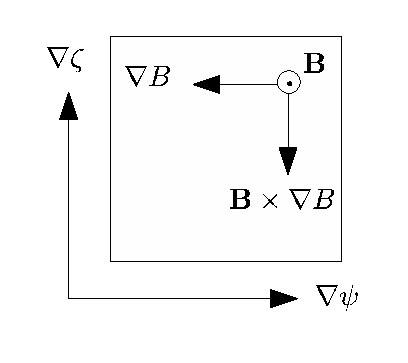
\includegraphics[width=0.3\textwidth]{directions.eps}
 \caption{\label{directions}Coordinate directions on the outboard
   plane ($s=0$) for $s_{\rm B}=1$, as output by the potential slices
   diagnostic \File{phi\#} with the coordinate labels for each point
   as output by \File{xphi} and \File{yphi} (the yphi coordinate label
   inverts the plot). For $s_{\rm B}=1$, the poloidal field is
   `upwards' ${\rm sign}(B_p \nabla \theta \cdot \nabla \zeta)= s_{\rm
     B}$. If in doubt, see Sec.~\ref{signs}.  Note that the `centre'
   of the flux tube is in the bottom left corner when output from the
   FFTs.}
 \end{center}
 \end{figure}
%This means as the matlab script mkmovie plots it.


\section{Summary: diagnostic outputs and their data format}
\label{sec.diagnos-data-format}

In GKW, most diagnostics are calculated inside the code at runtime (as
opposed to in post-processing).  The advantage of this approach is
that one does not need to store the full 5 dimensional distribution
functions at every timestep (which occupy a lot of disk space and are
difficult to transfer).  The disadvantage is that if a time dependent
diagnostic is not enabled or implemented before the run, that
information cannot later be retrieved without re-running the entire
simulation (final state diagnostics can always be retrieved by
restarting the code if the restart file is available).  One should
therefore think carefully about which diagnostics are required before
launching any expensive simulation.  One could argue that this
approach is suited to a world in which computation is cheap, but
storage and transfer are expensive.

The default set of time dependent diagnostics contains scalar time
traces (fluxes, growth rates) and 1D spectra, but no 2D or 3D
quantities.

GKW does contain a wrapper which allows to write output data
in various formats, according to the setting of \name{io_format} in
the input file.
\begin{description}
\item[\name{io_format='ascii'}] (also called 'formatted' output) All
  data is written to a collection of text files. Those can be read and
  analysed easily, and they are very portable. The ASCII format
  becomes impractical for higher dimensional and large amounts of data.

  For ascii and binary formats, diagnostic meta-data is output by the
  code to a simple text file \File{gkwdata.meta}.

\item[\name{io_format='binary'}] (also called 'raw' output) All data
  is written to binary files. Binary data consumes typically by a
  factor of about 6-10 less disk space than ascii data. Binary or hdf5
  (see below) format is therefore recommended if large amounts of data
  are produced.
\item[\name{io_format='hdf5'}] (also called 'structured' output), if
  \name{io_format='hdf5'} is set. This structured binary format is
  available if the code was compiled with the HDF5 library. If the
  HDF5 library was compiled with szip encoding support, then the GKW
  output data can be compressed (for now, there is only a hardcoded
  switch, see the comments).
  \\
%Issue 69    
  The HDF5 format allows to output diagnostic meta-data by associating
  attributes to datasets. These can be read by analysis
  scripts.  More and more metadata will be added in the near future, for
  discussions see \issue{69}. Note that
  \begin{itemize}
  \item If one tries to access HDF5 files during run, they may turn
    out to be invalid (not always though).
  \item Aborted runs may leave a corrupted HDF5 file. Usually then
    there are just no parameters in the file, sometimes datasets are
    missing and in rarer cases even the file as a whole is invalid.
  \item To produce the 3d fields and moments data and the 4d mode
    structure data, a MPI gather operation is performed and the output
    is written serially by just one process. For large runs with many
    processes this is likely not very performant. Instead, it is
    recommended to use MPI-IO binary output format then.
  \item At the time moment GKW supports only serial
    HDF5.
  \end{itemize}
\end{description}

In order to take advantage of the benefits of certain formats, GKW
knows also about mixed output:
\begin{description}
\item[\name{io_format='mixed'}] Most of the data (mainly scalar time
  traces and 1D spectra, \File{parallel.dat} final state
  eigenfunctions) is output to text files, whereas higher dimensional
  data is output to binary files.
\item[\name{io_format='hdf5+ascii'}] All data is output as with the
  'hdf5' setting. In addition, lowerdimensional data is output also to
  text files.
\end{description}

As long as there is not enough descriptive metadata attached to the
GKW diagnostic output data, we here summarize most of the GKW
diagnostic outputs in tables \ref{tab:diag-part1} and
\ref{tab:diag-part2} for 1D time traces, final state outputs, and 2D
time trace outputs.  A full listing of available diagnostics and
switches is documented in \doc{input.dat.sample}.  In the case of less
standard diagnostics it may be necessary to examine the source and
comments in the respective diagnostic module \src{diagnos_foo.F90} to
determine the exact order and meaning of the output quantities.

Generally, 2D diagnostics can be output by GKW at every timestep, or
at the end (``R or E'' in tables \ref{tab:diag-part1} and
\ref{tab:diag-part2}, switched by \name{xy_estep}). \\
When successive binary records for each timestep are stacked into one
file, this happens with (32 bit / 4 byte, usually)
integers before and after each record for the size of the binary
record (which will have Endianness of the hardware it was written on).
The data records can be
read into matlab with the script \matlab{read_file2d.m}.\\

Some slices are output at the point nearest the LFS, for
these a different location can be set with switch
\name{xy_slice_ipar}. 

\paragraph*{Reorganisation of diagnostics and the \name{io_legacy} switch:}
Note that there currently efforts to clean up GKW's diagnostics. This
includes renaming of some files, split up of datasets and change of
the order of the data, where necessary. The goal is to output data in
a more natural way which is easy to understand and to analyse.

In order to provide users for some time the possibility to keep using
their old analysis tools without larger changes, the switch
\name{io_legacy} was introduced.

\begin{landscape}
\begin{table}[hp!]
\begin{footnotesize}
\vspace{-2cm}
\begin{adjustwidth}{-1cm}{-2cm}
\centering 
\begin{tabular}{l|l|l|l|l|l|l}
 Filename / dataset name & Description & Quantity (norm.=normalised) & Size 
& when
& \parbox[t]{1cm}{Grid\\Files}
& \parbox[t]{1.5cm}{Namelist\\Switch}\\
\hline
%\File{foo} & [description] & [expression] & [rows,cols,..]  &B/R/E/O & [gridfiles] & [switch]\\
\hline\multicolumn{7}{ |c| }{\textbf{Module diagnos_growth_freq:}} \\
\File{dominant_growth_rate} & Dominant linear mode growth rate & $\gamma_{N}^{\rm max}$ & $N_t$  & R & & \\
\File{dominant_real_freq} & Dominant linear mode frequency & $\omega_N$ belonging to $\gamma_{N}^{\rm max}$& $N_t$  & R & & \\
\File{growth_rates.dat} & Growth rates of all linear modes & $\gamma_N$ &   & R & & \\
\File{frequencies.dat} & Frequencies of all linear modes & $\omega_N$ &   & R & & \\
\File{amplitudes.dat} & Amplitudes of all linear modes &  &  & R & & \\


\hline\multicolumn{7}{ |c| }{\textbf{Module diagnos_grid:}} \\
\File{time.dat} & timestamp (large time steps) & $t_N$ & $N_t$  & R & & \\
\File{sgrid} & s grid (parallel coordinate) & $s$ & $N_s$  & B & & \\
\File{krho} & Bi-normal wavevector grid & $(q / 2 \pi \psi) k_\zeta \rho_{\rm ref} = k_\perp(k_\psi=0,s=0) \rho_{\rm ref}$ & $N_x, N_{\rm mod}$& B & & \\
\File{kxrh} & Radial wavevector grid & $k_\psi \rho_{\rm ref}$ & $N_x, N_{\rm mod}$& B & & \\
\File{yphi} & Real space bi-normal grid & $ 2 \pi \psi (\zeta-\zeta_{\rm min})/q\rho_{\rm ref} = k_\theta \rho_{\rm ref}$ & $M_x,
M_{\rm mod}$ & B & & \\
\File{xphi} & Real space radial grid & $(\psi-\psi_{\rm min})/\rho_* = (r-r_{\rm min})/\rho_{\rm ref} $ & $M_x, M_{\rm mod}$ & B & & \\
\File{kx_connect} & Parallel boundary connections & Labelled in file & N/A& B & & \\
\hline\multicolumn{7}{ |c| }{\textbf{Module diagnos_mode_struct:}} \\
\File{phi} & es. potential & See Sec. \ref{sec.parallel}. & $N_{\rm MOD},  N_s, N_x$ & E and O & & \\
\File{Apar} &  & See Sec. \ref{sec.parallel}. & $N_{\rm MOD},  N_s, N_x$ & E and O & & \\
\File{Bpar} &  & See Sec. \ref{sec.parallel}. & $N_{\rm MOD},  N_s, N_x$ & E and O & & \\
\File{dens} & density fluctuations & See Sec. \ref{sec.parallel}. & $N_{\rm sp}, N_{\rm MOD},  N_s, N_x$ & E and O & & \\
\File{Tpar} & parall. temperature fluct. & See Sec. \ref{sec.parallel}. & $N_{\rm sp}, N_{\rm MOD},  N_s, N_x$ & E and O & & \\
\File{Tperp} & perp. temp. fluctuations & See Sec. \ref{sec.parallel}. & $N_{\rm sp}, N_{\rm MOD},  N_s, N_x$ & E and O & & \\
\File{vpar} & parallel flow fluctuations & See Sec. \ref{sec.parallel}. & $N_{\rm sp}, N_{\rm MOD},  N_s, N_x$ & E and O & & \\

\hline\multicolumn{7}{ |c| }{\textbf{Module diagnos_fields:}} \\
\File{kyspec} & Bi-normal mode potential spectrum &  $\sum_{k_\psi} \int_{s} |\hat \phi(k_\psi,k_\zeta,s)|^2 \, {\rm d}s $    &  $N_t,N_{\rm mod}$& R & & \\
\File{kyspec_em} & (Equivalent for $A_\parallel$ field) & $\sum_{k_\psi} \int_{s} |\hat A_\parallel(k_\psi,k_\zeta,s)|^2 \, {\rm d}s $ & $N_t,N_{\rm mod}$ & R\\
\File{kxspec(_em)} & Radial mode potential spectrum &  $\sum_{k_\zeta} \int_{s} |\hat \phi(k_\psi,k_\zeta,s)|^2 {\rm d}s $  & $N_t,N_x$  & R & & \\
\File{kyvort} & Bi-normal vorticity spectra &  $\sum_{k_\psi,sp} \int Z_{sp}|\hat f_{sp}(k_\psi,k_\zeta,s)|^2 \, {\rm d}^3 v \, {\rm d}s $  & $N_t,N_{\rm mod}$ & R & & \\

\File{kxvort} & Radial vorticity spectra &  $\sum_{k_\zeta,sp} \int Z_{sp} |\hat f_{sp}(k_\psi,k_\zeta,s)|^2 \, {\rm d}^3 v \, {\rm d}s $  & $N_t,N_x$ & R & & \\
\hline
\File{spc\#}  & ES potential spectrum (LFS) & $|\hat \phi(k_\psi,k_\zeta,s\approx0)|$ \ (norm.)& &R or E & \File{kxrh, krho} & \name{xy_phi} \\

\File{phi\#}  & ES potential slice (LFS) &  $\phi(\psi,\zeta,s\approx0)$ \ (norm.)&  &R or E & \File{xphi, yphi} & \name{xy_phi} \\

\File{apc\#}  & EM potential spectrum (LFS) &   $|\hat A_\parallel (k_\psi,k_\zeta,s\approx0)|$ \ (norm.)& &R or E & \File{kxrh, krho} & \name{xy_apar} \\

\File{apa\#}  & EM potential slice (LFS) &  $A_\parallel(\psi,\zeta,s\approx0)$\ (norm.) & &R or E & \File{xphi, yphi} & \name{xy_apar} \\

\File{bpc\#}  & EM field spectrum (LFS) &  $|\hat B_\parallel(k_\psi,k_\zeta,s\approx0)|$ \ (norm.)& &R or E & \File{kxrh, krho} & \name{xy_bpar} \\

\File{bpa\#}  & EM field slice (LFS) &  $B_\parallel(\psi,\zeta,s\approx0)$ \ (norm.)& &R or E & \File{xphi, yphi} & \name{xy_bpar} \\

\File{vok\#}  & Vorticity spectrum (FSA) &  $\sum_{s} \int |\hat f_{s}(k_\psi,k_\zeta)| d^3 v ds$ \ (norm.)& &R or E & \File{kxrh, krho} & \name{xy_vort}\\


\hline\multicolumn{7}{ |c| }{\textbf{Module diagnos_moments:}} \\
\File{ene[sp\#]_\#}  & Temp. pert. moment (LFS) &  $\sum_{sp} \int |\hat f_{s} v^2| d^3 v $ \ (norm.)& &R or E & \File{xphi, yphi} & \name{xy_temp} \\

\File{den[sp\#]_\#}  & Density pert. moment (LFS) &  $\int |\hat f_{s}| d^3 v $ \ (norm.)& &R or E & \File{xphi, yphi} & \name{xy_dens} \\

\File{pac[sp\#]_\#}  & Current pert. moment (LFS) &  $\int |\hat f_{s} | v_\parallel d^3 v $ \ (norm.)& &R or E & \File{xphi, yphi} & \name{xy_current} \\

\File{pac[sp\#]_\#}  & Current$^2$ pert. moment (LFS) &  $\int |\hat f_{s} | v_\parallel^2 d^3 v $ \ (norm.) & &R or E & \File{xphi, yphi} & \name{xy_current2} \\

\File{{den/ene}_spectra} & \parbox[t]{3.5cm}{Bi-normal spectral perturbation moments for each species} & $\sum_{k_\psi}\int_s \int \hat \alpha_{1,2} |\hat f_{sp}| {\rm d}^3v \, {\rm d}s $ & $N_{\rm mod},N_{sp}$ & & & \\

\end{tabular}
\end{adjustwidth}
\end{footnotesize}
\caption{
  Diagnostics output by GKW (Part 1), with \name{io_legacy=false}. The
  abbreviations denote output at the beginning (B), repeatedly (R), at the end
  (E) or other (O). FSA denotes Flux Surface Averaged quantities. LFS denotes quantities evaluated at the low field side, i.e. in the center of the $s$-grid.
}
\label{tab:diag-part1}
\end{table}
\end{landscape}

\begin{landscape}
\begin{table}[hp!]
\begin{footnotesize}
\vspace{-2cm}
\begin{adjustwidth}{-1cm}{-1cm}
\centering 
\begin{tabular}{l|l|l|l|l|l|l}
 Filename / dataset name & Description & Quantity (norm.=normalised) & Size 
& \parbox[t]{2cm}{beginning (B),\\ repeatedly (R),\\ at the end (E)}
& \parbox[t]{1cm}{Grid\\Files}
& \parbox[t]{1.5cm}{Namelist\\Switch}\\
\hline
\hline\multicolumn{7}{ |c| }{\textbf{Module diagnos_moments:}} \\
\File{dens_kyzero_xs[sp\#]_\#}    & Density pert. moment ($k_\zeta = 0$) &  $\int |\hat f_{sp}| d^3 v $ \ (norm.)            & &R  & \File{xphi, sgrid} & \name{xs_kyzero_dens} \\
\File{current_kyzero_xs[sp\#]_\#} & Current pert. moment ($k_\zeta = 0$) &  $\int |\hat f_{sp}| v_\parallel d^3 v $ \ (norm.)& &R  & \File{xphi, sgrid} & \name{xs_kyzero_current} \\
\File{ene_kyzero_xs[sp\#]_\#}     & Energy pert. moment ($k_\zeta = 0$)  &  $\int |\hat f_{sp}| v^2 d^3 v $ \ (norm.)& &R  & \File{xphi, sgrid} & \name{xs_kyzero_ene} \\
\File{ene_par_kyzero_xs[sp\#]_\#}     & Parallel energy pert. moment ($k_\zeta = 0$)  &  $\int |\hat f_{sp}| v_\parallel^2 d^3 v $ \ (norm.)& &R  & \File{xphi, sgrid} & \name{xs_kyzero_ene_par} \\
\File{ene_perp_kyzero_xs[sp\#]_\#}     & Perpendicular energy pert. moment ($k_\zeta = 0$)  &  $\int |\hat f_{sp}| v_\perp^2 d^3 v $ \ (norm.)& &R  & \File{xphi, sgrid} & \name{xs_kyzero_ene_perp} \\
\File{phi_ga_fm_kyzero_xs[sp\#]_\#}     & Gyro-averaged (using $F_M$) el.-stat. potential  ($k_\zeta = 0$)  &  $\int |\hat F_{M,sp}| \langle \hat \phi \rangle d^3 v $ \ (norm.)& &R  & \File{xphi, sgrid} & \name{xs_kyzero_phi_ga_fm} \\

\hline\multicolumn{7}{ |c| }{\textbf{Module diagnos_fluxes:}} \\
%\File{fluxes.dat} & Total $v_E$ fluxes $(i=1,2,3)$ by species  & ${\cal I}_i=\sum_{k_\zeta} \sum_{k_\psi} \int_{s} \bar{\cal I}_i \, {\rm d}s$  & $3N_{sp}$ & R & & \\
\File{p/e/vflux_es} & Total $v_E$ particle/heat/momentum flux by species  & ${\cal I}_i=\sum_{k_\zeta} \sum_{k_\psi} \int_{s} \bar{\cal I}_i \, {\rm d}s$  & $N_t,N_{sp}$ & R & \File{time} & \\
\File{p/e/vflux_es_lab} & Corresponding Lab frame fluxes & ${\cal I}_i+d{\cal I}_i$  & $N_t,N_{sp}$ & R & \File{time} & \\
%\File{eflux_es} & Total $v_E$ heat flux by species  & ${\cal I}_2=\sum_{k_\zeta} \sum_{k_\psi} \int_{s} \bar{\cal I}_2 \, {\rm d}s$  & $N_t,N_{sp}$ & R & \File{time} & \\
%\File{vflux_es} & Total $v_E$ momentum flux by species  & ${\cal I}_3=\sum_{k_\zeta} \sum_{k_\psi} \int_{s} \bar{\cal I}_3 \, {\rm d}s$  & $N_t,N_{sp}$ & R & \File{time} & \\
\File{p/e/vflux_apar} & Total $A_\parallel$ particle/heat/momentum flux by species  & ${\cal J}_i=\sum_{k_\zeta} \sum_{k_\psi} \int_{s} \bar{\cal J}_i \, {\rm d}s$  & $N_t,N_{sp}$ & R &  \File{time} & \\
\File{p/e/vflux_apar_lab} &  Corresponding Lab frame fluxes & ${\cal J}_i+d{\cal J}_i$  & $N_t,N_{sp}$ & R &  \File{time} & \\
%\File{eflux_apar} & Total $A_\parallel$ heat flux by species  & ${\cal J}_2=\sum_{k_\zeta} \sum_{k_\psi} \int_{s} \bar{\cal J}_2 \, {\rm d}s$  & $N_t,N_{sp}$ & R &  \File{time} & \\
%\File{vflux_apar} & Total $A_\parallel$ momentum flux by species  & ${\cal J}_3=\sum_{k_\zeta} \sum_{k_\psi} \int_{s} \bar{\cal J}_3 \, {\rm d}s$  & $N_t,N_{sp}$ & R &  \File{time} & \\
\File{p/e/vflux_bpar} & Total $\nabla B_\parallel$ particle/heat/momentum flux by species  & ${\cal K}_i=\sum_{k_\zeta} \sum_{k_\psi} \int_{s} \bar{\cal K}_i \, {\rm d}s$  & $N_t,N_{sp}$ & R &  \File{time} & \\
\File{p/e/vflux_bpar_lab} & Corresponding Lab frame fluxes  & ${\cal K}_i + d{\cal K}_i$  & $N_t,N_{sp}$ & R &  \File{time} & \\
%\File{eflux_bpar} & Total $\nabla B_\parallel$ heat flux by species  & ${\cal K}_2=\sum_{k_\zeta} \sum_{k_\psi} \int_{s} \bar{\cal K}_2 \, {\rm d}s$  & $N_t,N_{sp}$ & R &  \File{time} & \\
%\File{vflux_bpar} & Total $\nabla B_\parallel$ momentum flux by species  & ${\cal K}_3=\sum_{k_\zeta} \sum_{k_\psi} \int_{s} \bar{\cal K}_3 \, {\rm d}s$  & $N_t,N_{sp}$ & R &  \File{time} & \\

\File{{p/e/v}flux_spectra} & Bi-normal spectral $v_E$ flux for each species & $\sum_{k_\psi} \int_{s} \bar {\cal I}_i(k_\psi,k_\zeta) \, {\rm d}s$ & $N_t,N_{\rm mod},N_{sp}$ & R & & \\

\File{{p/e/v}flux_xspec}  & Radial spectral $v_E$ fluxes for each species & $\sum_{k_\zeta} \int_{s} \bar {\cal I}_i(k_\psi,k_\zeta) \, {\rm d}s$  & $N_t,N_{\rm mod},N_{sp}$   & R & & \\

\File{{p/e}flux_(em_)sup} & \parbox[t]{3.5cm}{Bi-normal spectral flux suprema for each species} & $\hat {\cal I}_i(k_\zeta), \hat {\cal J}_i(k_\zeta) $ & $N_t,N_{\rm mod},N_{sp}$ & R & & \\

\hline
\File{PFlesr[sp\#]_\#}  & ES radial particle flux (LFS) & ${\cal I}_1(\psi,\zeta,s\approx0)$\ (norm.)& & R or E & \File{xphi, yphi} & \name{xy_fluxes_P} \\

\File{EFlesr[sp\#]_\#}  & ES radial energy flux (LFS) & ${\cal I}_2(\psi,\zeta,s\approx0)$ \ (norm.)& & R or E & \File{xphi, yphi} & \name{xy_fluxes} \\

\File{VFlesr[sp\#]_\#}  & ES radial momentum flux (LFS) & ${\cal I}_3(\psi,\zeta,s\approx0)$ \ (norm.)& & R or E & \File{xphi, yphi} & \name{xy_fluxes_V} \\

\File{[P/E/V]Fl\underline{em}r[sp\#]_\#}  & EM flutter fluxes as above (LFS) &  $J_i(\psi,\zeta,s\approx0)$ \ (norm.) & & R or E & \File{xphi, yphi} & \name{+ xy_fluxes_em} \\

\File{[P/E/V]Fl\underline{bp}r[sp\#]_\#}  & EM comp. fluxes as above (LFS) &  $K_i(\psi,\zeta,s\approx0)$ \ (norm.)& & R or E & \File{xphi, yphi} & \name{+ xy_fluxes_bpar} \\

\File{[P/E/V]F\underline{S}[es/em/bp]r[sp\#]_\#}  & All fluxes as abv., but (FSA) &  $\int I_i/J_i/K_i(\psi,\zeta) ds$ \ (norm.)& & R or E & \File{xphi, yphi} & \name{+ xy_fluxes_fsa} \\

\File{[P/E/V]F[l/S][es/em/bp]\underline{p}[sp\#]_\#}  & Binormal fluxes as abv. (LFS/FSA)&  N/A & & R or E & \File{xphi, yphi} & \name{+ xy_fluxes_bi} \\

\File{[P/E/V]Fl[es/em/bp]\underline{k}[sp\#]_\#}  & Radial fluxes spectra (FSA) &  $\int I_i/J_i/K_i(k_\psi,k_\zeta) ds$ \ (norm.)& & R or E & \File{kxrh, krho} &  \name{+ xy_fluxes_k} \\

\hline\multicolumn{7}{ |c| }{\textbf{Module diagnos_fluxes_vspace:}} \\
\File{fluxes_det.dat} & \parbox[t]{4cm}{5D fluxes for each species, \\including $\ud^3X$ and $\ud^3v$}& $\Big(\bar{\cal I}_i + \bar{\cal J}_i +  \bar{\cal K}_i\Big)(k_\psi,k_\zeta,s,\mu,v_\parallel)$  & \parbox[t]{2cm}{binary, $N_{v_\parallel} N_\mu N_s\\ N_\psi N_{mod} N_{sp} i,$\\$i=1,2,3$}& E & & \name{lfluxes_detail} \\
\hline

\File{[p/e/v]fluxes_vspace[sp\#]_\#}  & Fluxes in velocity space (FSA) &  $\int I_i/J_i/K_i(v_\parallel,\mu) ds$ \ (norm.)& &R or E & \File{distr[1/2]} & \name{lfluxes_vspace} \\

%\hline\multicolumn{7}{ |c| }{\textbf{Module diagnos_rad:}} \\
%\hline\multicolumn{7}{ |c| }{\textbf{Module diagnos_velspace:}} \\
%\hline\multicolumn{7}{ |c| }{\textbf{Module diagnos_energetics:}} \\
\hline\multicolumn{7}{ |c| }{\textbf{Module diagnos_f:}} \\
\File{distr*.dat}   & 2D velocity space output of 1 mode. & 1,2 grids, 3 Re$({\hat g}(s=0))$, 4 Im$({\hat g}(s=0))$ & $N_\mu$, $N_{v_\parallel}$ & E & & \\
%\hline\multicolumn{7}{ |c| }{\textbf{Module diagnos_stresses:}} \\
%\hline\multicolumn{7}{ |c| }{\textbf{Module diagnos_zfshear:}} \\
%\hline\multicolumn{7}{ |c| }{\textbf{Module diagnos_eng:}} \\
%\hline\multicolumn{7}{ |c| }{\textbf{Module diagnos_nonlin_transfer:}} \\

\hline\multicolumn{7}{ |c| }{\textbf{Output by other parts of the code:}} \\
\File{parfun.dat} & Perpendicular wavevector & $k_\perp\rho_{\rm ref}$ & $2,N_s N_{\rm mod} N_x$& B & & \\
\File{par.dat} & Curvature and Coriolis functions & $k_\perp\rho_{\rm ref}$ , ${\cal D}^\psi k_\psi + {\cal
D}^\zeta k_\zeta$, ${\cal H}^\psi k_\psi + {\cal H}^\zeta k_\zeta$, & $3,N_s N_{\rm mod} N_x$& B & & \\
\File{geom.dat} & Geometry tensors & Labelled in file & N/A& B & & \\
\File{FDS}        & Restart distribution function  & binary (see Sec. \ref{sec.restart})& E & & \\
\File{FDS.dat}    & Additional restart information & Ascii namelists (see Sec. \ref{sec.restart}) & E & & \\
\File{Coll_params.dat} & Collision frequencies & Labelled in file & N/A & B & & \\
\File{cfdens.dat} & Centrifugal poloidal density variations & $s$, $R/L_{\rm n, sp}^E(s)$, $exp(-\cfenn)_{\rm sp}(s), \theta$ &  $2 N_{\rm sp} + 2$ & B & & \\
\end{tabular}
\end{adjustwidth}
\end{footnotesize}
\caption{
  Diagnostics output by GKW (Part 2) , with \name{io_legacy=false}.
}
\label{tab:diag-part2}
\end{table}
\end{landscape}

\begin{landscape}
\begin{table}[hp!]
\begin{footnotesize}
\vspace{-2cm}
\begin{adjustwidth}{-1cm}{-2cm}
\centering 
\begin{tabular}{l|l|l|l|l|l|l}
 Filename & Description & Quantity (norm.=normalised) & Cols,(Rows) 
& \parbox[t]{2cm}{beginning (B),\\ repeatedly (R),\\ at the end (E)}
& \parbox[t]{1cm}{Grid\\Files}
& \parbox[t]{1.5cm}{Namelist\\Switch}\\
\hline
\hline\multicolumn{7}{ |c| }{\textbf{Module diagnos_growth_freq:}} \\
\File{time.dat} & Dominant linear mode growth rate & $t_N, \gamma_{N}^{\rm max}, \omega_N$ & 3  & R & & \\
\File{growth.dat} & Growth rates of all linear modes & $\gamma_N$ &   & R & & \\
\hline\multicolumn{7}{ |c| }{\textbf{Module diagnos_mode_struct:}} \\
\File{parallel.dat} & Parallel mode structure & See Sec. \ref{sec.parallel}. & $N_{\rm MOD} N_x N_s N_{\rm sp}$ & E & & \\
\hline\multicolumn{7}{ |c| }{\textbf{Module diagnos_moments:}} \\
\File{{den/ene}_spectra} & \parbox[t]{3.5cm}{Bi-normal spectral perturbation  moments for each species} & $\sum_{k_\psi}\int_s \int \hat \alpha_{1,2} |\hat f_{sp}| {\rm d}^3v \, {\rm d}s $ & $N_{\rm mod}N_{sp}$ & & & \\
\hline\multicolumn{7}{ |c| }{\textbf{Module diagnos_fluxes:}} \\
\File{fluxes.dat} & Total $v_E$ fluxes $(i=1,2,3)$ by species  & ${\cal I}_i=\sum_{k_\zeta} \sum_{k_\psi} \int_{s} \bar{\cal I}_i \, {\rm d}s$  & $3N_{sp}$ & R & & \\
\File{fluxes_lab.dat} & Total Lab frame $v_E$ fluxes $(i=1,2,3)$ by species  & ${\cal I}_i + d{\cal I}_i$  & $3N_{sp}$ & R & & \\
\File{fluxes_em.dat} & Total $\delta B$ fluxes $(i=1,2,3)$ by species  & ${\cal J}_i=\sum_{k_\zeta} \sum_{k_\psi} \int_{s} \bar{\cal J}_i \, {\rm d}s$  & $3N_{sp}$ & R & & \\
\File{fluxes_em_lab.dat} & Total Lab frame $\delta B$ fluxes $(i=1,2,3)$ by species  & ${\cal J}_i+d{\cal J}_i$  & $3N_{sp}$ & R & & \\
\File{fluxes_bpar.dat} & Total $\nabla B_{1 \parallel}$ fluxes $(i=1,2,3)$ by species  & ${\cal K}_i=\sum_{k_\zeta} \sum_{k_\psi} \int_{s} \bar{\cal K}_i \, {\rm d}s$  & $3N_{sp}$ & R & & \\
\File{fluxes_bpar_lab.dat} & Total Lab frame $\nabla B_{1 \parallel}$ fluxes $(i=1,2,3)$ by species  & ${\cal K}_i+d{\cal K}_i$  & $3N_{sp}$ & R & & \\
\end{tabular}
\end{adjustwidth}
\end{footnotesize}
\caption{
  Legacy diagnostics output by GKW, with \name{io_legacy=true}. This table shows
  output datasets which differ from the ones described in
  tables \ref{tab:diag-part1} and \ref{tab:diag-part2} which
  are associated with \name{io_legacy=false}.
}
\label{tab:diag-legacy}
\end{table}

\end{landscape}

\newpage
 
\section{Island torque and stabilization by the parallel current}

A diagnostic especially useful for tearing mode dynamics is the one giving the torque and the stabilization
 by the parallel current, namely $T_\varphi$ and $\Delta_{\rm pol}$, respectively. These quantities are defined as follows, under
the assumption of a non rotating island
\begin{equation}
T_\varphi \propto \int_{-L_x/2}^{L_x/2}\, dx\, \int_{-\pi}^{\pi}\, d\zeta_0\,\,J_\parallel\sin\left(\kappa_{\zeta,\rm isl}\zeta_0\right)
\label{torque}
\end{equation}
\begin{equation}
\Delta_{\rm pol} \propto \int_{-L_x/2}^{L_x/2}\, dx\, \int_{-\pi}^{\pi}\, d\zeta_0\,\,J_\parallel\cos\left(\kappa_{\zeta,\rm isl}\zeta_0\right)
\label{deltaprime}
\end{equation}
where $L_x$ is the width of the simulation box in the radial direction, the variable $\zeta_0$ is the
helical co-ordinate in the absence of rotation and $J_\parallel$ is the gyro-centre parallel
current, given by
\begin{equation}
J_\parallel = \sum_{s}eZ_s\int_{\mathbb{R}^3} \, d^3\mathbf{v}\, v_\parallel \delta f_s
\end{equation}
with $\delta f_s$ the perturbed distribution function of the gyro-centres of species $s$.
Note that multiplying equation \ref{torque} by $-i$
and adding the resulting expression to equation \ref{deltaprime} yields
\begin{equation}
\Delta_{\rm pol} - i T_\varphi \propto \sum_{s}eZ_s\int_{-L_x/2}^{L_x/2}\, dx\, \int_{-\pi}^{\pi}\, d\zeta_0\, \int_{\mathbb{R}^3} \, d^3\mathbf{v} \, v_\parallel \delta f_s\, \exp\left(-i\kappa_{\zeta,\rm isl}\zeta_0\right)
\end{equation}
where we can distinguish the Fourier mode $\hat{\delta f_s}_{isl}\equiv\hat{\delta
f_s}\left(\kappa_\zeta=\kappa_{\zeta,\rm isl}\right)\propto\int_{-\pi}^{\pi}\, d\zeta_0\, \delta f_s \, \exp\left(-i\kappa_{\zeta,\rm isl}\zeta_0\right)$, with $\kappa_{\zeta,\rm isl}$ being the mode
 of the island in the binormal direction. Therefore, we can write
\begin{equation}
\Delta_{\rm pol} - i T_\varphi \propto \sum_{s}eZ_s\int_{-L_x/2}^{L_x/2}\, dx\, \int_{\mathbb{R}^3} \, d^3\mathbf{v} \, v_\parallel \hat{\delta f_s}_{\rm isl}
\end{equation}
A rotating island is usually imposed or obtained self-consistently in GKW. This means that the island is not
 always in the middle of the simulation box in the binormal direction. However, the above expressions are
 obtained assuming that the island is centered and therefore need to be corrected by multiplying
 by the phase $\exp\left(i\int_0^t \,dt' \omega_{\rm isl}\right)$, where $\omega_{\rm isl}$ is the rotation of the island, which results
 in the definition of the co-ordinate $\zeta = \zeta_0 - \int_0^t\, dt'\omega_{\rm isl}$. Note that in the absence
 of rotation, the amplitude of the vector potential $A_\parallel$ is real, due to the fact that a pure
 $\cos\left(\kappa_\zeta \zeta\right)$ is represented in GKW by a real amplitude of $A_\parallel$. Therefore,
 any departure from a real amplitude in $A_\parallel$ implies a rotation $\omega_{\rm isl}$, which can be calculated as
\begin{equation}
\int_0^t \, dt' \omega_{\rm isl} = \arctan\left(\frac{\Im\left(A_\parallel\right)}{\Re\left(A_\parallel\right)}\right)
\end{equation}
leading to the expression
\begin{equation}
\mathcal{T}\equiv\Delta_{\rm pol} - i T_\varphi \propto \sum_{s}eZ_s\int_{-L_x/2}^{L_x/2}\, dx\, \int_{\mathbb{R}^3} \, d^3\mathbf{v} \, v_\parallel \hat{\delta f_s}_{\rm isl}\exp\left(i\int_0^t \, dt' \omega_{\rm isl}\right)
\end{equation}

Finally, the torque and instability parameter are calculated as
\begin{equation}
T_\varphi = -\Im\left(\mathcal{T}\right)
\end{equation}
\begin{equation}
\Delta_{\rm pol} = \Re\left(\mathcal{T}\right)
\end{equation}

These two quantities are output in the files \File{torque.dat} and \File{deltaprime.dat}, respectively. The first column corresponds to
 the values for the ions and the second column to the values for the electrons.

\pagebreak

\section{Entropy (module \texttt{diagnos\_energetics} and \texttt{diagnos\_eng})}

% To cite ?
% Candy PoP 13, 032310 (2006):  Does this not relate directly to what we have ?
% Krommes 94

\subsection{Definition of the Total Entropy of the Simulated Box}\label{sec:entr-simul-box}
Let $p(\mathbf{X},v_\parallel, \mu) \in [0,1]$ be a probability density function.

One can define the functional
\begin{equation}
  \label{eq:bgs-entropy}
  S = -\int\!\ud^3x\ud^3v p\ln(p\cdot c_d),\qquad c_d = \mathrm{const.}
\end{equation}
and show that this expression has properties of the thermodynamical entropy (see e.g.\ the book of Jelitto 1989). It is therefore called ``statistical entropy'' or Shannon-Jaynes-entropy or Pauli-entropy or Boltzmann-Shannon-Gibbs (BGS) entropy. 
 A constant $c_d$ is formally needed in \ref{eq:bgs-entropy} to make the logarithm dimensionless \cite{DUN07} but it can be set equal to 1. Note that the integral in \ref{eq:bgs-entropy} is over the whole system, i.e.\ derived integrals below, on quantities of the simulated model, are taken over the whole simulation box. 

A ``relative entropy'' functional can be defined in the form
\begin{equation}
  \label{eq:relative-entropy}
  S = -\int\!\ud^3x\ud^3v\ p\ln \frac{p}{q}
\end{equation}
This functional characterizes the distribution $p$ with respect to a certain reference probability density function $q \in [0,1]$ . 


Maximization of the relative entropy $S$ under the constraint
\begin{align}\label{eq:maximizationSconstraint}
  1 = \int\ud\mathbf{x}\ud\mathbf{v}\,p(\mathbf{x},\mathbf{v})
\end{align}
leads to the condition
\begin{align}
  0 = 1 + ln\frac{p}{q} + \alpha
\end{align}
and thus
\begin{align}\label{eq:maximizationSp}
  p = q\cdot\exp[-(1+\alpha)]\
\end{align}
the distribution which corresponds to the extremum of the functional depends on the reference. With the assumption that the reference PDF $q$ fulfills
\ref{eq:maximizationSconstraint}, one applies this constraint \ref{eq:maximizationSconstraint} to \ref{eq:maximizationSp} and finds then $\alpha = -1$ and so
\begin{align}
  p = q ,
\end{align}
that means the entropy has its extremum for $p=q$.
Variation of the relative entropy under other constraints, using a reference which fulfills those, leads to the condition $p = q$ by the same argument.

% Is it not the neoclassical canoncial Maxwellian that is really the maximum entropy distribution ?
For a PDF describing an ensemble of classical particles, the distribution which maximizes the entropy under two contraints (normalisation of the distribution and given kinetic energy average) is the Maxwellian. 
For our purposes, we put therefore $f_{tot}$ in place of $p$ and the reference
distribution is chosen to be the Maxwell distribution in velocity space and to
describe particle trapping (and possibly centrifugal trapping) in position space.
This Maxwellian distribution function is denoted with $F_M$ and is given in equation \eqref{eq:maxwell}.
\begin{equation}
  \label{eq:relative-entropy-with-f}
  S = -\int\!\ud^3X\ud^3v f_{tot}\ln \frac{f_{tot}}{F_M}
\end{equation}
A state of maximum entropy then corresponds to $f_{tot} = F_M$. In the $\delta f$ model, where the distribution is split into $f_{tot} = F_M + f$, this means that the distribution perturbation vanishes in the thermodynamic equilibrium: $f = 0$.

Furthermore, it can be shown \cite{DUN07} that in contrast to the BGS entropy \ref{eq:bgs-entropy} given first, maximizing the relative entropy \ref{eq:relative-entropy} leads to the same distribution function, independently of the coordinate system. This is an important property if we want to investigate systems relaxing towards equilibrium in the field aligned coordinate system in which the gyrokinetic model is formulated. The invariance under coordinate transformations of the maximum-entropy principle associated with the relative entropy notion \ref{eq:relative-entropy} guarantees that the distribution $f_{tot} = F_M$ really corresponds to the maximum value of the entropy, and not another distribution, e.g.\ by multiplication with a factor.

Reduction of the perturbation $|f|$ means growth of the entropy $S$, i.e.\ the system moves towards thermodynamic equilibrium. On the contrary, processes that grow fluctuations $|f|$ effectively diminish the entropy of the system and keep it away from equilibrium, which is by definition the macrostate of maximum entropy.

We set $f_{tot} = F_M + f$ and expand around $f=0$: 
\begin{align}
  (F_M + f)\ln\frac{F_M + f}{F_M} &= (F_M + f)\left[0 + \frac{1}{F_M + f}|_{f=0}f^1 + \frac{1}{2}\frac{-1}{(F_M + f)^2}|_{f=0}f^2 + \ldots\right] \nonumber\\
  &= 0 + f + \frac{f^2}{F_M} - \frac{1}{2}\frac{f^2}{F_M} + \ldots \nonumber\\
  &= 0 + f + \frac{1}{2}\frac{f^2}{F_M} + \ldots
                     % \ln\frac{F_M + f}{F_M} &=  0 + \frac{f}{F_M} - \frac{1}{2}\frac{f^2}{F_M^2}\ldots + \ldots
\end{align}
Then \ref{eq:relative-entropy-with-f} becomes
\begin{align}
  \label{eq:def-entropy}
  S \approx -\int\!\ud^3X\ud^3v (f + \frac{1}{2}\frac{f^2}{F_M}) = -\frac{1}{2}\int\!\ud^3X\ud^3v\frac{f^2}{F_M}
\end{align}
where the integral of the fluctuation $f$ vanishes. 
$S$ in \ref{eq:def-entropy} is a small-amplitude approximation to the plasma entropy.  % \cite{krommes94}
 Again, one can see that reduction of $|f|$ means increase of the entropy $S$.

In its normalized form  \ref{eq:def-entropy} is 
\begin{equation}
  \label{eq:entropy}
  S \approx -\frac{1}{2}\int\!\ud^3X\ud^3v\frac{f^2}{F_M} = \rho_*^2 \frac{v_{thref}}{R_{ref}}n_{R_0}\underbrace{\left(-\frac{1}{2}\int\!\ud^3X\ud^3v_N\frac{f_N^2}{F_{MN}}\right)}_{S_N}
\end{equation}
In the normalized balance equation \ref{eq:entropy-balance} the reference quantities are dropped, but the smallness parameter $\rho_*$ is kept for illustration.

The quantity $H = -S$ is a measure of the intensity of the fluctuations in the distribution.% \cite{candywaltz06}
\begin{equation}
  \label{eq:intensity}
  H \approx \frac{1}{2}\int\!\ud^3X\ud^3v\frac{f^2}{F_M} = \rho_*^2 \frac{v_{thref}}{R_{ref}}n_{R_0}\underbrace{\left(\frac{1}{2}\int\!\ud^3X\ud^3v_N\frac{f_N^2}{F_{MN}}\right)}_{H_N}
\end{equation}
%Being a positive functional of the distribution, the intensity $H$ is an energy-like quantity \cite{krommes94}.
%FIXME This may be interesting when looking at the growth of unstable fluctuations? \cite{krommes94}

To emphasise, the fluctuation intensity $H$ is found to be \emph{increasing} in the simulations of a system driven out of equilibrium by applied thermodynamic forces (temperature and density gradient). Accordingly the entropy $S=-H$ is found to decrease.

\subsection{Entropy Balance\label{sec:entr-balance}}

\subsubsection*{General procedure} 
One starts from the normalized gyrokinetic equation given in section \ref{equations}, multiplies every term with $\frac{f}{F_M}$ and integrates over the box volume and velocity space.

In this section, all quantities are normalized, but we omit the index $N$ here. Moreover, only the electrostatic case is considered, so that $g = f$ for the purposes of this section.

\begin{align}\label{eq:entropy-balance}  
\rho_*^2\int\!\ud^3X\ud^3v\frac{f}{F_M}\Big[\pd{g}{t} +\mathrm{I} + \mathrm{II} + \mathrm{III} + \mathrm{IV} + \mathrm{V} + \mathrm{VI} + \mathrm{VII} + \mathrm{VIII}\Big] = 0 
\end{align}

\subsubsection*{Regard the terms separately}
One can recover $\pd{\ }{t} H$ in the very first integral.
\begin{align}
  \label{eq:dSdt}
  \rho_*^2\int\!\ud^3X\ud^3v\frac{f}{F_M}\pd{g}{t} &= \rho_*^2\int\!\ud^3X\ud^3v\frac{1}{F_M}\frac{1}{2}\pd{f^2}{t} \nonumber\\
&= \pd{H}{t} = - \pd{S}{t}
\end{align}

The linear $\mathbf{E}\times\mathbf{B}$-drift term V yields
\begin{align} 
  \rho_*^2\int\!\ud^3X\ud^3v\frac{f}{F_M}\ \mathrm{V} & = \rho_*^3\int\!\ud^3X \Bigg[-\frac{1}{L_n}\Gamma_N^\psi - Q_N^\psi\frac{1}{L_T}\nonumber\\
  &\quad +\frac{3}{2}\frac{1}{L_T}\Gamma^\psi - \frac{\mathcal{E}_R}{T_R}\frac{1}{L_T}\Gamma^\psi +\nonumber\\
  &\quad - \frac{2}{T_R}\Pi_\varphi^\psi u^\prime
  - 2\frac{m_R}{T_R}\Omega_N^2\mathcal{L}\,\Gamma^\psi \Bigg]
\end{align}
At the moment these six terms are output separately by the code, but
very likely they will be combined in the near future to fewer, more
symmetric quantities.

The Landau-Damping terms VI and VII give non-vanishing contributions,
too. In combination with the Poisson equation, they can be
rewritten as
\begin{align}
  \rho_*^2\int\!\ud^3X\ud^3v\frac{f}{F_M}\Big[\mathrm{VII} + \mathrm{VIII}\Big] &= \int\ud^3X \pd{}{t} \sum_s\int\ud^3v \frac{Z_s^2}{2T_s^2}F_M\left(\phi^2(\mathbf{x}) - \Ga{\phi}^2 \right) \\
 \text{and $W_s$ is defined such that} &= \pd{}{t}\sum_sW_s \\
 W_{N,s} = {}& \int\ud^3X_N \int\ud^3v_N \frac{Z_s^2}{2T_{R,s}^2}F_{MN}\left(\phi_N^2 -  \Ga{\phi_N}^2\right)   \label{eq:W}
\end{align}
If only ion dynamics is simulated and electrons are treated
adiabatically, the index $s$ above only runs over ion species and the
term $W_{N,e}$ for the electrons is different.
\begin{align}
\pd{}{t}W_{N,e,adia}
{}={}& \pd{}{t}\int\ud^3X_N \phi_N \int\ud^3v_N\frac{Z_e}{T_{R,e}}\iGa{f_{eN}} \nonumber\\
{}={}& \pd{}{t}\int\ud^3X_N \phi_N \frac{Z_e}{T_{R,e}}n_R\frac{Z_e}{T_{R,e}}\left(\phi_N - \fsa{\phi_N} \right) \nonumber\\
{}={}& \int\ud^3X_N  n_R\frac{Z_e^2}{2T_{R,e}^2}\left(
 \pd{\phi_N^2}{t} - 2\phi_N\pd{}{t}\fsa{\phi_N}
 \right)
\end{align}
And with $\fsa{.}=\fsa{.}(\psi,\zeta)$ and $T_{R,e}^2$ being constant
with respect to the parallel direction, one can write
\begin{align}
{}={}& \int\ud\psi\ud\zeta J_X   n_R\frac{Z_e^2}{2T_{R,e}^2}\left(
\pd{\fsa{\phi_N^2}}{t} -
 2\fsa{\phi_N}\pd{}{t}\fsa{\phi_N}
 \right)\\
{}={}& \int\ud\psi\ud\zeta J_X   n_R\frac{Z_e^2}{2T_{R,e}^2}\left(
 \pd{\fsa{\phi_N^2}}{t} -
\pd{\fsa{\phi_N}^2}{t}
  \right) \\
{}={}& \pd{}{t}\int\ud\psi\ud\zeta J_X  n_R\frac{Z_e^2}{2T_{R,e}^2}\left(
  \fsa{\phi_N^2} -
 \fsa{\phi_N}^2 
\right) 
\ .
\label{eq:W-corr-adia}
\end{align}

% A rotating plasma knows about a further correction for the adiabatic
% electron contribution, also due to a modification of the Poisson
% equation.
% \begin{align}
%  \pd{}{t} W_{N,e,adia,rot}{}={}& \pd{}{t} \int\ud\psi\ud\zeta J_X   n_R\frac{Z_e}{T_{R,e}^2}\left(
% % Z_e\frac{1}{2}\fsa{\phi_N}^2
% %  \right.\nonumber\\&\qquad\qquad \left.
% % -Z_e\frac{1}{2}\fsa{\phi_N^2}
% + \fsa{\phi_N\mathcal{E}_{R,e}}
% \right)
% \end{align}


\subsection{Resulting entropy balance equation\label{sec:result-entropy-balance}}

The terms of the entropy balance equation which were very briefly presented
in section \ref{sec:entr-balance}, and the numerical diffusion terms,
summed over all species make up the following balance equation.
\begin{align}
  0 &= \sum_s\pd{}{t}(H_s + \overbrace{W_s}^{\text{\makebox[0pt]{from VII and VIII}}}) + \sum_s\Big(\overbrace{\text{contrib. from turb. fluxes}}^{\text{\makebox[0pt]{from linear ExB drift V;}}} + \overbrace{\text{\ \ contrib. from neoclass. fluxes}}^{\text{\makebox[0pt]{from VI, but this is ignored and not implemented}}}  + \nonumber \\
  &\quad{}-\mathcal{D}_{f\parallel} - \mathcal{D}_{v_\parallel} - \mathcal{D}_{\perp} \Big) - \sum_s\int\!\ud^3X\ud^3v_N\frac{f_N}{F_{MN}}\mathcal{C}_N
\end{align}
To be more explicit, in terms of entropy this equation reads
\begin{align}  \label{eq:result-entropy-balance}
 \sum_s\pd{}{t}(S_s - W_s) =&\sum_s\Big(\int\!\ud^3X \Bigg[-\frac{1}{L_n}\Gamma_N^\psi - Q_N^\psi\frac{1}{L_T}
  +\frac{3}{2}\frac{1}{L_T}\Gamma^\psi - \frac{\mathcal{E}_R}{T_R}\frac{1}{L_T}\Gamma^\psi 
  - \frac{2}{T_R}\Pi_\varphi^\psi u^\prime
  - 2\frac{m_R}{T_R}\Omega_N^2\mathcal{L}\,\Gamma^\psi \Bigg]\nonumber\\
 &\quad\quad-\mathcal{D}_{f\parallel} -\mathcal{D}_{v_\parallel} -\mathcal{D}_{\perp}\Big)
- \sum_s\int\!\ud^3X\ud^3v_N\frac{f_N}{F_{MN}}\mathcal{C}_N
\end{align}
and in terms of free energy
\begin{align}
  & \pd{}{t}\sum_s(-T_{R,s}S_{N,s} + E_{\chi,N,s}) = {}\nonumber\\
&\quad\sum_sT_{R,s}\Big(\int\!\ud^3X \Bigg[\frac{1}{L_n}\Gamma_N^\psi + Q_N^\psi\frac{1}{L_T}
  -\frac{3}{2}\frac{1}{L_T}\Gamma^\psi + \frac{\mathcal{E}_R}{T_R}\frac{1}{L_T}\Gamma^\psi
  + \frac{2}{T_R}\Pi_\varphi^\psi u^\prime
  + \frac{m_R}{T_R}\Omega_N^2\mathcal{L}\,\Gamma^\psi \Bigg]\nonumber\\
 &\quad\quad+\mathcal{D}_{f\parallel} +\mathcal{D}_{v_\parallel} +\mathcal{D}_{\perp}\Big)
 %+ \sum_sT_{R,s}\int\!\ud^3X_N\ud^3v_N\frac{h_N}{F_{MN}}\mathcal{C}_N
+ \sum_s\mathcal{D}_{C,s}
\end{align}
where $E_{\chi,S}=W_sT_{R,s}$.

In a system driven out of equilibrium the fluctuations grow, that is,
the entropy gets smaller (i.e.\ more negative). The time derivative on
the left side is therefore negative. This corresponds to the fluxes
and the gradient lengths defined here being positive and the numerical
dissipation terms $\mathcal{D}_i$ being negative.

In a statistically steady state, the left side of this equation
vanishes. The entropy sinks from the fluxes are then balanced by the
numerical dissipation terms.

\subsection{Output quantities of the diagnostic}\label{sec:entr-output}

If \texttt{lcalc_energetics} in the diagnostics namelist is switched
on, the code will produce a number of files related to the entropy
balance equation:

The quantities in the entropy balance equation \ref{eq:result-entropy-balance}
 correspond directly to the output of the \texttt{energetics()} diagnostic.

\begin{align}
   \mathtt{dt\_entr} + \mathtt{dt\_entr\_field} =& -\Big(\mathtt{entr\_src01} + \mathtt{entr\_src02} + \mathtt{entr\_src03} \nonumber\\
& \quad + \mathtt{entr\_src04} + \mathtt{entr\_src05} + \mathtt{entr\_src06}
\nonumber\\
 &\quad\quad + \mathtt{entr\_num\_dis} + \mathtt{entr\_num\_vp} + \mathtt{entr\_num\_perp} \nonumber\\
& \quad\quad + \mathtt{entr\_coll}\Big)
\end{align}
To clarify the signs, note the definition
\begin{align}
  \pd{}{t}\sum_s\left(-W_{N,s}\right) = \mathtt{dt\_entr\_field} \ .
\end{align}

In order to check the balance one can sum both sides and see how well
they eliminate each other.

\begin{align}
&   \mathtt{dt\_entr} + \mathtt{dt\_entr\_field} +\Big(\mathtt{entr\_src01} + \mathtt{entr\_src02} + \mathtt{entr\_src03} \nonumber\\
& \quad + \mathtt{entr\_src04} + \mathtt{entr\_src05} + \mathtt{entr\_src06}
\nonumber\\
 &
%\underbrace{
\quad\quad + \mathtt{entr\_num\_dis} + \mathtt{entr\_num\_vp} + \mathtt{entr\_num\_perp} + \mathtt{entr\_coll}\Big)
%}_{\mathtt{total}} 
\overset{?!}{=} 0
\end{align}


\pagebreak

\section{Zonal potential evolution (module \texttt{diagnos\_zonal\_evo})}
\label{zonal-potential-evolution}

The zonal potential is the flux-surface averaged potential and is defined by
\begin{equation}
\{\phi \} = \sum_{k_\psi} \underbrace{ \int \mathrm{d}s~\hat \phi (k_\psi, k_\zeta=0,s) }_{\{\hat \phi \}(k_\psi)} \exp(\mathrm{i} k_\psi \psi / \rho_\ast),
\end{equation}
where the spectral representation (see Sec.~\ref{sec:spectral}) is applied and $\{\hat \phi \}(k_\psi)$ defines the complex Fourier coefficient of the zonal potential with radial wave vector $k_\psi$. 
An evolution equation for the zonal potential can be derived from the Poisson equation (\ref{Poisson}).
The time derivative of the inverted and flux-surface averaged $k_\zeta = 0$ part of this equation reads
\begin{equation}
\label{eq:dt-inverted-poisson}
\frac{\partial \{ \hat \phi \}(k_\psi)}{\partial t} = -\int \mathrm{d} s ~ \frac{1}{\mathcal{P}}  \sum_{sp} Z_{sp} n_{R,sp} 2 \pi B  \int \mathrm{d} v_{\parallel} \int \mathrm{d} \mu ~ \biggl[J_0(k_\perp\rho_{sp}) \frac{\partial \hat g_{sp}}{\partial t} \biggr]_{\mathbf{k}=(k_\psi,k_\zeta=0)}
\end{equation}
where
\begin{equation}
\mathcal{P} = \sum_{sp} \frac{n_{R,sp} Z_{sp}^2}{T_{R,sp}} [ \Gamma_0(b_{sp}) -1].
\end{equation}
Here, the notation $[ \hat G ]_{\mathbf{k}=(k_\psi,k_\zeta=0)}$ means that the argument $\hat G$ has to be evaluated at $k_\zeta = 0$. \\
The module \texttt{diagnos\_zonal\_evo} calculates various contributions to the time evolution of the zonal potential.
For this purpose, the time derivative of the perturbed modified distribution function $\partial_t \hat g_{sp}$, entering the right hand side of Eq.~(\ref{eq:dt-inverted-poisson}), is substituted by the individual terms (I-XI) on the right hand side of the gyrokinetic equation (\ref{eqs:complete-set}).
This procedure yields several linear and nonlinear contributions to the evolution of the zonal potential.
The corresponding diagnostic output is discussed in Sec.~\ref{zevo-output-quantities}.


\subsection{Vanishing terms}
This part will be more specific about individual linear terms entering through the time derivative of the modified distribution.
Closer inspection shows that several terms vanish.\\
%
First, the velocity space integral of the trapping term (term IV) is carried out:
\begin{align}
& \int \mathrm{d} \mu \int \mathrm{d} v_\parallel ~ J_0[k_\perp \rho(\mu) ] v_{R} \left(\mu B {\cal G} + {1 \over 2} \pd{\cfenn}{s} {\cal F} \right) \pd{\hat f}{v_\parallel} \\
= & \int \mathrm{d} \mu  ~ J_0[k_\perp \rho(\mu) ]  v_{R} \left(\mu B {\cal G} + {1 \over 2} \pd{\cfenn}{s} {\cal F} \right) \int \mathrm{d} v_\parallel \pd{\hat f}{v_\parallel} \\
= & \int \mathrm{d} \mu ~  J_0[k_\perp \rho(\mu) ]  v_{R} \left(\mu B {\cal G} + {1 \over 2} \pd{\cfenn}{s} {\cal F} \right) \biggl[ \hat f\biggr]_{-\infty}^{+\infty} \\
= & ~0.
\end{align}
It has been used that $\partial_{v_\parallel} \hat f$ is the only quantity with $v_\parallel$-dependence, allowing for a separatation of the velocity space integration. 
Since the perturbed distribution has to vanish for $v_\parallel \rightarrow \pm \infty$ the integration over parallel velocity space yields zero. \\
%
Second, the inner product of the ExB-drift and the parallel motion along perturbed field lines, i.~e., $\mathbf{v}_\chi$, with the gradient of the maxwellian (term V) is concentrated on (neglecting the Sung terms that are higher order in $\rho_\ast$):
\begin{align}
& \int \mathrm{d} \mu \int \mathrm{d} v_\parallel ~J_0(k_\perp \rho) \mathrm{i}k_\alpha \hat \chi|_{k_\zeta = 0} {\cal E}^{\alpha \psi} \biggl [ {1 \over L_n} + {m_R \Omega ^2 \over T_R}{\cal L} + E_T {1 \over L_T} + {2 v_{\parallel} \over  v_{R}} {R B_t \over B} u^\prime \biggr ] F_{M} = \\
= & \int \mathrm{d} \mu \int \mathrm{d} v_\parallel ~ J_0(k_\perp \rho) \mathrm{i}k_\psi \hat \chi|_{k_\zeta = 0} {\cal E}^{\psi \psi} \biggl [ {1 \over L_n} + {m_R \Omega ^2 \over T_R}{\cal L} + E_T {1 \over L_T} + {2 v_{\parallel} \over  v_{R}} {R B_t \over B} u^\prime \biggr ] F_{M} = \\
= & ~ 0.
\end{align}
It has been used that the $k_\zeta = 0$ part of the modified potential is considered, i.~e., $\hat \chi|_{k_\zeta = 0} = \hat \chi (k_\psi, k_\zeta=0, s)$, such that the multiplication with $k_\zeta$ vanishes.
Furthermore, ${\cal E}^{\psi \psi} = 0$. \\
In a well resolved numerical simulation the above described terms should vanish.
The remaining terms are non-zero, in general, and may contribute to the evolution of the zonal potential.


\subsection{Constructing $k_\psi$-$k_\zeta'$-spectra from Hermitian symmetry}
\label{zevo-kxky-spectra}
The nonlinear terms of the gyrokinetic equation allow for the evolution of the zonal potential through the nonlinear interaction of perturbations with finite $k_\zeta'$.
Here, $k_\zeta'$ refers to the binormal wave vector of modes that interact through the nonlinearity.
It has to be distinguished from the wave vector $k_\zeta$ used in Eq.~(\ref{eq:dt-inverted-poisson}) that refers to the perturbation that is generated by the nonlinear interaction, i.~e., here the $k_\zeta = 0$ mode.
The Hermitian symmetry of the spectrum allows to construct $k_\psi$-$k_\zeta'$-spectra of the contribution of the nonlinear terms to the zonal potential evolution. \\
The nonlinear term entering Eq.~(\ref{eq:dt-inverted-poisson}) can be formally written in position space by
    \begin{equation}
    \mathcal{N}(\psi) = \frac{1}{L_\zeta} \int_0^{L_\zeta} \mathrm{d} \zeta A(\psi, \zeta) B(\psi,\zeta),
    \label{eq:formal-nonlinearity}
    \end{equation}
where $L_\zeta$ is the box size in the $\zeta$-direction.
For simplicity the $s$-dependence and integration are neglected.
Since the domain is periodic in $\zeta$, only the constant part of the integrand contributes.
This is equivalent to the condition $k_\zeta = 0$ on the right hand side of Eq.~(\ref{eq:dt-inverted-poisson}). \\
The perturbed fields entering the nonlinearity are real quantities and, therefore, their Fourier respresentation satisfies Hermitian symmetry (see also Sec.~\ref{sec.parseval-correction})
    \begin{equation}
    G(\psi, \zeta) = \hat G (\psi,k_\zeta'=0) + \sum_{k_\zeta' > 0} \biggl[ \hat G (\psi,k_\zeta') \exp(\mathrm{i} k_\zeta' \zeta/\rho_\ast) +  \hat G^\ast (\psi,k_\zeta') \exp(-\mathrm{i} k_\zeta' \zeta/\rho_\ast) \biggr],
    \label{eq:hermitian-spectrum}
    \end{equation}
where $G \in [A, B]$ and the superscript "$\ast$" denotes the complex conjugate.
Since the part that is constant in $\zeta$ contributes to the integral in Eq.~(\ref{eq:formal-nonlinearity}) only, one finds
    \begin{align}
    \mathcal{N}(\psi)  = & \frac{1}{L_\zeta} \int_0^{L_\zeta} \mathrm{d} \zeta \sum_{k_\zeta'>0} \sum_{k_\zeta''>0} \biggl[ \hat A(\psi,k_\zeta') \hat B^\ast(\psi,k_\zeta'') \exp[\mathrm{i} (k_\zeta' - k_\zeta'')\zeta'/\rho_\ast] \nonumber \\
                         & + \hat A^\ast(\psi,k_\zeta') \hat B(\psi,k_\zeta'') \exp[-\mathrm{i} (k_\zeta' - k_\zeta'')\zeta'/\rho_\ast] \biggr] \label{eq:zevo-hermitian-1}\\
            = & \sum_{k_\zeta'>0} \biggl[ \hat A(\psi,k_\zeta') \hat B^\ast(\psi,k_\zeta') + \hat A^\ast(\psi,k_\zeta') \hat B(\psi,k_\zeta') \biggr] \label{eq:zevo-hermitian-2}\\
            = & 2 \sum_{k_\zeta'>0} \mathrm{Re}[\hat A(\psi,k_\zeta') \hat B^\ast(\psi,k_\zeta')].\label{eq:zevo-hermitian-3}
    \end{align}
Terms proportional to $\exp[\mathrm{i}(k_\zeta'+k_\zeta'') \zeta'/\rho_\ast]$ in expression (\ref{eq:zevo-hermitian-1}) vanish due to periodicity in $\zeta$ and due to $k_\zeta',~k_\zeta'' > 0$.
In expression (\ref{eq:zevo-hermitian-2}) it has been used that $\int_0^{L_\zeta} \mathrm{d}\zeta~\exp[\mathrm{i}(k_\zeta'-k_\zeta'') \zeta'/\rho_\ast] = \delta_{k_\zeta',k_\zeta''}$, where the latter is the Kronecker delta.
The factor $2$ in expression (\ref{eq:zevo-hermitian-3}) is what is called \texttt{parseval\_correction} in the code. \\
In case of the nonlinearity of the gyrokinetic equation
    \begin{equation}
    A = \rho_\ast^2 \mathcal{E}^{\psi \zeta} \pd{\chi}{\zeta} \hspace{20pt} B = \pd{g}{\psi}
    \end{equation}
or 
    \begin{equation}
    A = -\rho_\ast^2 \mathcal{E}^{\psi \zeta}\pd{\chi}{\psi} \hspace{20pt} B = \pd{g}{\zeta},
    \end{equation}
where $\chi$ is defined in Eq.~(\ref{eq:chi-normalized}).
Finally, the time evolution of the $\mathbf{k}=(k_\psi,k_\zeta=0)$ mode of the distribution function due to the nonlinearity then reads
    \begin{equation}
    \label{eq:zevo-hermitian}
    \Biggl[ \pd{\hat g}{t}\Big|_\mathrm{NL}\Biggr]_{\mathbf{k}=(k_\psi,k_\zeta=0)} (k_\psi) = \sum_{k_\zeta'} \underbrace{\mathcal{T}_\psi \biggl\{\rho_\ast 2 \mathcal{E}^{\psi \zeta} \mathrm{Re} \biggl[ \mathrm{i} k_\zeta' \hat \chi(\psi,k_\zeta') \biggl( \pd{\hat g (\psi,k_\zeta')}{\psi} \biggr)^\ast - \pd{\hat \chi(\psi,k_\zeta')}{\psi} \biggl( \mathrm{i} k_\zeta' \hat g(\psi,k_\zeta') \biggr)^\ast \biggr]\biggr\}}_{[\partial_t \hat g |_\mathrm{NL}]_{\mathbf{k}=(k_\psi,k_\zeta=0)}  (k_\psi,k_\zeta')}.
    \end{equation}
Here, $\mathcal{T}_\psi$ denotes a Fourier transform in $\psi$. 
The factor $\rho_\ast$ in Eq.~(\ref{eq:zevo-hermitian}) vanishes after the Fourier transform, since $\partial_\psi \hat{g} \rightharpoondown (\mathrm{i} k_\psi /\rho_\ast) \hat{g}$ and $\partial_\psi \hat{\chi} \rightharpoondown (\mathrm{i} k_\psi /\rho_\ast) \hat{\chi}$ . 
Note that Eq.~(\ref{eq:zevo-hermitian}) also defines the contribution from interacting modes with wave vector $k_\zeta'$, i.~e., $[\partial_t \hat g |_\mathrm{NL}]_{\mathbf{k}=(k_\psi,k_\zeta=0)}  (k_\psi,k_\zeta')$.
The dependency on $k_\psi$ (not $k_\psi'$) is explicitly given within parentheses and refers to the radial wave vector of the mode that is generated nonlinearly. \\
Following the procedure described in Sec.~\ref{zonal-potential-evolution}, Eq.~(\ref{eq:zevo-hermitian}) is substituted for $\partial_t \hat g_{sp}$ on the right hand side of Eq.~(\ref{eq:dt-inverted-poisson}).
%Note that the condition $k_\zeta = 0$ in Eq.~(\ref{eq:dt-inverted-poisson}) translates to the requirement that only the constant part of the integrant in Eq.~(\ref{eq:formal-nonlinearity}) contributes.
%It is, therefore, implicitly satisfied by the expression given in Eq.~(\ref{eq:zevo-hermitian}).
It is worth to stress again that $k_\zeta'$ in Eq.~(\ref{eq:zevo-hermitian}) specifies the wave vector of the modes that interact nonlinearly, while $k_\zeta$ correponds to the mode that is generated by this nonlinear interaction process, i.~e., here a mode with $k_\zeta = 0$. 

    
    
\subsection{Output quantities}
\label{zevo-output-quantities}
Per default (\texttt{lcalc\_zonal\_evo}) the diagnostic outputs $k_\psi$-spectra of the zonal potential $\{\hat \phi \}$, the time derivative of the zonal potential $\partial_t \{\hat \phi \}$, the contribution of the sum of all linear terms of the gyrokinetic equation (including numerical dissipation and collisions, if active) and the individual nonlinear contributions (if active) to the zonal potential evolution (\ref{eq:dt-inverted-poisson}).
See Tab.~\ref{tab:diagnos-zonal-evo-output} for a list of the output files.
The output file \File{zevo03\_phi\_kx\_[real,imag]} is associated to the ExB-nonlinearity [$\phi$-term of $\chi$ in Eq.~(\ref{eq:chi-normalized})], the output file \File{zevo03\_apar\_kx\_[real,imag]} to the magnetic flutter nonlinearity [$A_\parallel$-term of $\chi$ in Eq.~(\ref{eq:chi-normalized})] and the output file \File{zevo03\_bpar\_kx\_[real,imag]} to the magnetic field compression nonlinearity [$B_\parallel$-term of $\chi$ in Eq.~(\ref{eq:chi-normalized})].
A numerical simulation should always satisfy
\begin{align}
\File{dt\_zphi\_kx\_[real,imag]} & = \File{zevo\_lin\_kx\_[real,imag]} + \File{zevo03\_phi\_kx\_[real,imag]} \nonumber \\
                                 & + \File{zevo03\_apar\_kx\_[real,imag]} + \File{zevo03\_bpar\_kx\_[real,imag]},
\end{align}
provided the time step is small enough for an accurate numerical estimation of the time derivative of $\{\hat \phi \}$ and provided numerical instabilities are absent. \\
A detailed output of $k_\psi$-spectra of the individual linear contributions to the zonal potential evolution is provided by the namelist switch \texttt{zevo\_detail}.
The nomenclature of the output files (see Tab.~\ref{tab:diagnos-zonal-evo-output}) follows the numbering of the individual terms of the complete set of equations described in Sec.~\ref{equations}.  
The sum of the individual linear contributions yields the combined linear output
\begin{align}
\File{zevo\_lin\_kx\_[real,imag]} & = \File{zevo01\_kx\_[real,imag]} + \File{zevo02\_kx\_[real,imag]} \nonumber \\
                                  & + \File{zevo04\_kx\_[real,imag]} + \File{zevo05\_kx\_[real,imag]} \nonumber \\
                                  & + \File{zevo07\_kx\_[real,imag]} + \File{zevo08\_kx\_[real,imag]} \nonumber \\
                                  & + \File{zevo10\_kx\_[real,imag]} + \File{zevo11\_kx\_[real,imag]} \nonumber \\
                                  & + \File{zevo\_dpar\_kx\_[real,imag]} + \File{zevo\_dvp\_kx\_[real,imag]} \nonumber \\
                                  & + \File{zevo\_dperp\_kx\_[real,imag]} + \File{zevo\_coll\_kx\_[real,imag]}.
\end{align}
\textit{WARNING: The calculation of the individual linear contributions is memory consuming, since it requires the allocation of multiple linear terms matrices! Depending on the problem size, the number of processors may have to be increased.} \\
The namelist switch \texttt{zevo\_xy\_spec} allows for the output of $k_\psi$-$k_\zeta'$-spectra of the nonlinear contributions to the zonal potential evolution (see Tab.~\ref{tab:diagnos-zonal-evo-output} for the output file naming).
This feature exploits the Hermitian symmetry of the binormal spectrum (see also Sec.~\ref{zevo-kxky-spectra}).
The corresponding output relates to the default output through
\begin{align}
\File{zevo03\_phi\_kx\_[real,imag]} & = \sum_{k_\zeta'} \File{zevo03\_phi\_kxky\_[real,imag]} \\
\File{zevo03\_apar\_kx\_[real,imag]} & = \sum_{k_\zeta'} \File{zevo03\_apar\_kxky\_[real,imag]} \\
\File{zevo03\_bpar\_kx\_[real,imag]} & = \sum_{k_\zeta'} \File{zevo03\_bpar\_kxky\_[real,imag]}.
\end{align}
In the above equations the expression $\sum_{k_\zeta'}$ denotes a sum over the $k_\zeta'$ dimension of the respective output file.
\textit{WARNING: The calculation of the $k_\psi$-$k_\zeta'$-spectral output is computationally expensive. 
If not mandatory, run performance might be improved by deactivation of} \texttt{zevo_xy_spec}.

\begin{landscape}
\begin{table}
\begin{center}
\begin{tabular}{c|c|c|c|c}
\textbf{Namelist switch}    & \textbf{File name}                     & \textbf{Additional requirements}   & \textbf{Size} & \textbf{Grid Files}\\
\hline \hline
 \texttt{lcalc\_zonal\_evo} & \File{zphi\_kx\_[real,imag]}           &                                    & $N_\mathrm{t},~N_x$ & \File{time}, \File{kxrh} \\
                            & \File{dt\_zphi\_kx\_[real,imag]}       &                                    & $N_\mathrm{t},~N_x$ & \File{time}, \File{kxrh}\\
                            & \File{zevo\_lin\_kx\_[real,imag]}      &                                    & $N_\mathrm{t},~N_x$ & \File{time}, \File{kxrh}\\
                            & \File{zevo03\_phi\_kx\_[real,imag]}    & \texttt{nonlinear}+\texttt{nlphi}  & $N_\mathrm{t},~N_x$ & \File{time}, \File{kxrh}\\
                            & \File{zevo03\_apar\_kx\_[real,imag]}   & \texttt{nonlinear}+\texttt{nlapar} & $N_\mathrm{t},~N_x$ & \File{time}, \File{kxrh}\\
                            & \File{zevo03\_bpar\_kx\_[real,imag]}   & \texttt{nonlinear}+\texttt{nlbpar} & $N_\mathrm{t},~N_x$ & \File{time}, \File{kxrh}\\
 \hline
 \texttt{lcalc\_zonal\_evo} & \File{zevo01\_kx\_[real,imag]}         &                                    & $N_\mathrm{t},~N_x$ & \File{time}, \File{kxrh}\\
 +\texttt{zevo\_detail}     & \File{zevo02\_kx\_[real,imag]}         &                                    & $N_\mathrm{t},~N_x$ & \File{time}, \File{kxrh}\\
                            & \File{zevo04\_kx\_[real,imag]}         &                                    & $N_\mathrm{t},~N_x$ & \File{time}, \File{kxrh}\\
                            & \File{zevo05\_kx\_[real,imag]}         &                                    & $N_\mathrm{t},~N_x$ & \File{time}, \File{kxrh}\\
                            & \File{zevo07\_kx\_[real,imag]}         &                                    & $N_\mathrm{t},~N_x$ & \File{time}, \File{kxrh}\\
                            & \File{zevo08\_kx\_[real,imag]}         &                                    & $N_\mathrm{t},~N_x$ & \File{time}, \File{kxrh}\\
                            & \File{zevo10\_kx\_[real,imag]}         & \texttt{nlbpar}                    & $N_\mathrm{t},~N_x$ & \File{time}, \File{kxrh}\\
                            & \File{zevo11\_kx\_[real,imag]}         & \texttt{nlbpar}                    & $N_\mathrm{t},~N_x$ & \File{time}, \File{kxrh}\\
                            & \File{zevo\_dpar\_kx\_[real,imag]}     &                                    & $N_\mathrm{t},~N_x$ & \File{time}, \File{kxrh}\\
                            & \File{zevo\_dvp\_kx\_[real,imag]}      &                                    & $N_\mathrm{t},~N_x$ & \File{time}, \File{kxrh}\\
                            & \File{zevo\_dperp\_kx\_[real,imag]}    &                                    & $N_\mathrm{t},~N_x$ & \File{time}, \File{kxrh}\\
                            & \File{zevo\_coll\_kx\_[real,imag]}     & \texttt{collisions}                & $N_\mathrm{t},~N_x$ & \File{time}, \File{kxrh}\\ 
 \hline
 \texttt{lcalc\_zonal\_evo} & \File{zevo03\_phi\_kxky\_[real,imag]}  & \texttt{nonlinear}+\texttt{nlphi}  & $N_\mathrm{t},~N_x,~N_\mathrm{mod}$ & \File{time}, \File{kxrh}, \File{krho} \\
 +\texttt{zevo\_xy\_spec}   & \File{zevo03\_apar\_kxky\_[real,imag]} & \texttt{nonlinear}+\texttt{nlapar} & $N_\mathrm{t},~N_x,~N_\mathrm{mod}$ & \File{time}, \File{kxrh}, \File{krho}\\
                            & \File{zevo03\_bpar\_kxky\_[real,imag]} & \texttt{nonlinear}+\texttt{nlbpar} & $N_\mathrm{t},~N_x,~N_\mathrm{mod}$ & \File{time}, \File{kxrh}, \File{krho}\\
\end{tabular}
\caption{This table lists the output of the module \name{diagnos\_zonal\_evo}.}
\label{tab:diagnos-zonal-evo-output}
\end{center}
\end{table}
\end{landscape}


% related to auctex mode and latex-preview-mode in Emacs:
%%% Local Variables:
%%% mode: latex
%%% TeX-master: "doc"
%%% End:

\chapter{Benchmarks} 

% Benchmarks to Add (even if just the reference):

% Edge shortfall case: AUG
% Edge shortfall case: DIII-D
% Casson MAST cases
% Dickinson MAST MTM case (EPS 2013)
% Henderson MAST case (EPS 2013)
% Guttenfelder / Hornsby MTM case
% Guttenfelder / Buchholz NSTX case
% Cottier QualizKiz cases
% Self-Benchmarks for the flux tube nonspectral version:
%   Linear, RH, nonlinear
% NEMORB global benchmarks


In this section we describe a set of benchmarks. 
The benchmark cases have been chosen to maximise the effect of each of the different implemented 
terms as much as possible.
Together they give evidence for the correct implementation of the entire model. 
Linear benchmarks have been made against the GS2 code which is well established. 
Indeed the model equations are equivalent, with the exception that GKW includes the effect of a 
rigid body toroidal rotation, while GS2 does not. The implementation is to some extent similar;
both 
use a spectral approach for the plane perpendicular to the magnetic field, and finite differences for 
the other directions. 
The main difference lies in the velocity space discretisation where GKW uses $(v_\parallel, \mu)$
coordinates, whereas GS2 uses pitch angle and energy.  The GS2 velocity grid allows an efficient
implicit time integrator, while the default grid of GKW is suitable for an explicit time integrator
which facilitates parallelisation.  Also the finite difference scheme used
for GKW in the benchmarks is fourth order while GS2 has a second order scheme. 
In this section all quantities have been converted to use gyro-Bohm units. 

\section{Linear Benchmarks\label{linearbenchmarks}} 

The standard benchmark for linear problems is the growth rate of the Ion Temperature Gradient 
mode (ITG) as a function of the poloidal wave vector $k_\theta \rho_s$ for the so-called 
Cyclone base case \cite{DIM00} ($q = 1.4$, $\hat s = 0.78$, $\epsilon = 0.19$, $R / L_T = 6.9$, 
$R/L_n = 2.2$, $T_e / T_i = 1$, electro-static (zero $A_\parallel$), and adiabatic electrons). 
The growth rate for this case is shown in the right panel of Fig.~\ref{fig:cyclone-linear} as a function 
of $k_\theta\rho_s$ for various values of the normalised ion temperature gradient ($R/L_T = 6.9$,
8.28 10.35, 12.44, and 15.18) calculated with both GKW and GS2. 
As can be seen from the figure, good agreement is obtained. 
The left panel, furthermore, shows the comparison of the potential as a function of the coordinate 
along the field line ($s$) for both codes. 

\begin{figure}[htb] 
\begin{center}
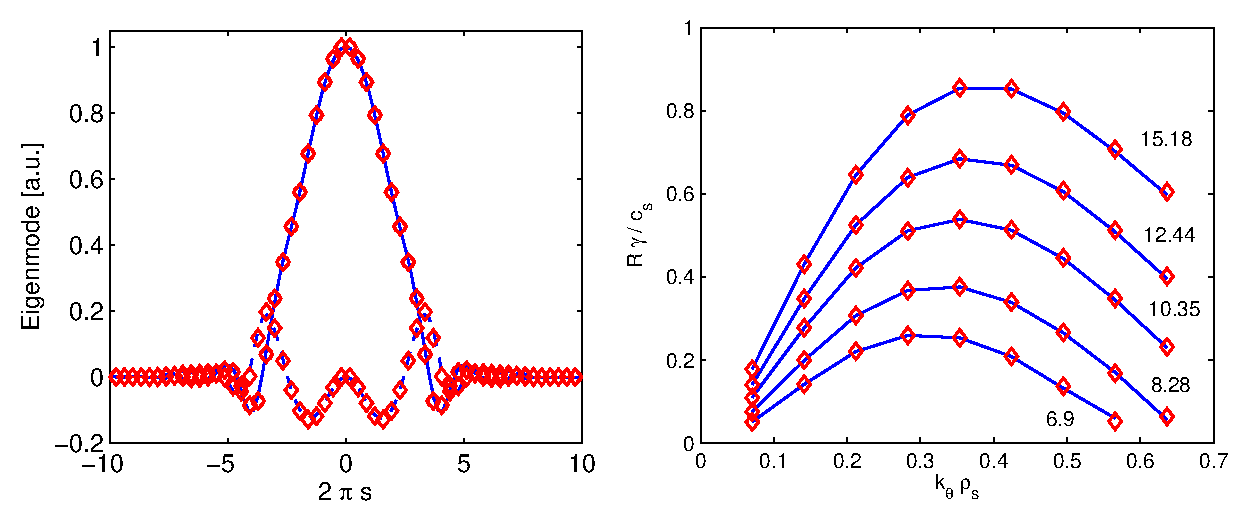
\includegraphics[width=14truecm]{cyclone-base-linear3.eps}
\caption{Left: mode structure of the Cyclone base case. The full line is the 
real part and the dotted line is the imaginary part of the potential calculated with GS2. 
The corresponding results of GKW are given by the diamonds. Right: growth rate as a function 
of $k_\theta \rho_s$ for various values of $R/L_{Ti}$ (numbers given in the figure). The full 
lines give the results of GS2 while the diamonds are the corresponding results of GKW.} 
\label{fig:cyclone-linear}
\end{center}
\end{figure}  

For nonlinear runs the proper response of the zonal flows is of utmost importance. 
The standard benchmark \cite{CAN03,JEN05,JOL07} that addresses the physics of the zonal flow / geo-acoustic 
mode is the Rosenbluth-Hinton test which was described analytically in Ref. \cite{HINROS}. 
In this benchmark the initial condition is an ion density 
perturbation with a finite (small) radial wave vector, and no dependence on either $s$ or $\zeta$.  
The adiabatic electron response is used, keeping the correction due to the flux surface average 
of the potential. The density perturbation generates a potential perturbation and excites the so
called geo-acoustic mode. This mode is damped and a small residual poloidal flow remains. Fig. 
\ref{zonalfig} gives the potential perturbation as a function of time. The relevant parameters used for this 
benchmark are $q = 1.3$, $\epsilon = 0.05$, $k_\psi \rho_s = 0.02$, electrostatic, collisionless. 
Rather large grid sizes ($N_s = 128$ and $N_{v_\parallel} = 128$) are used to avoid the recurrence 
problem \cite{CAN03}. The residual potential is given by the equation 
\begin{equation} 
{ \phi (t= \infty) \over \phi (t= 0) } = {1 \over 1 + q^2 \Theta / \epsilon^2} \qquad 
{\rm with} \qquad \Theta = 1.6 \epsilon^{3/2} + 0.5 \epsilon^2 + 0.36 \epsilon^{5/2} 
\end{equation}
The original derivation of Ref. \cite{HINROS} is accurate to lowest order in $\epsilon$ only, i.e. 
it retained only the first term $(1.6 \epsilon^{3/2})$ in $\Theta$. 
The higher order terms have been calculated in Ref.~\cite{XIA06}. 
For the parameters of the simulation shown in the left panel the residue is $\phi(t = \infty) / \phi(t= 0) 
= 0.0713$ smaller than the result of Ref. \cite{HINROS} (0.0764) but in very good agreement with the 
results of Ref. \cite{XIA06} (0.0710). The right panel shows the residue as a function of $\epsilon$. 
Good agreement with the analytic theory is obtained provided the finite $\epsilon$ effects are kept.  
\begin{figure}[htb] 
\begin{center}
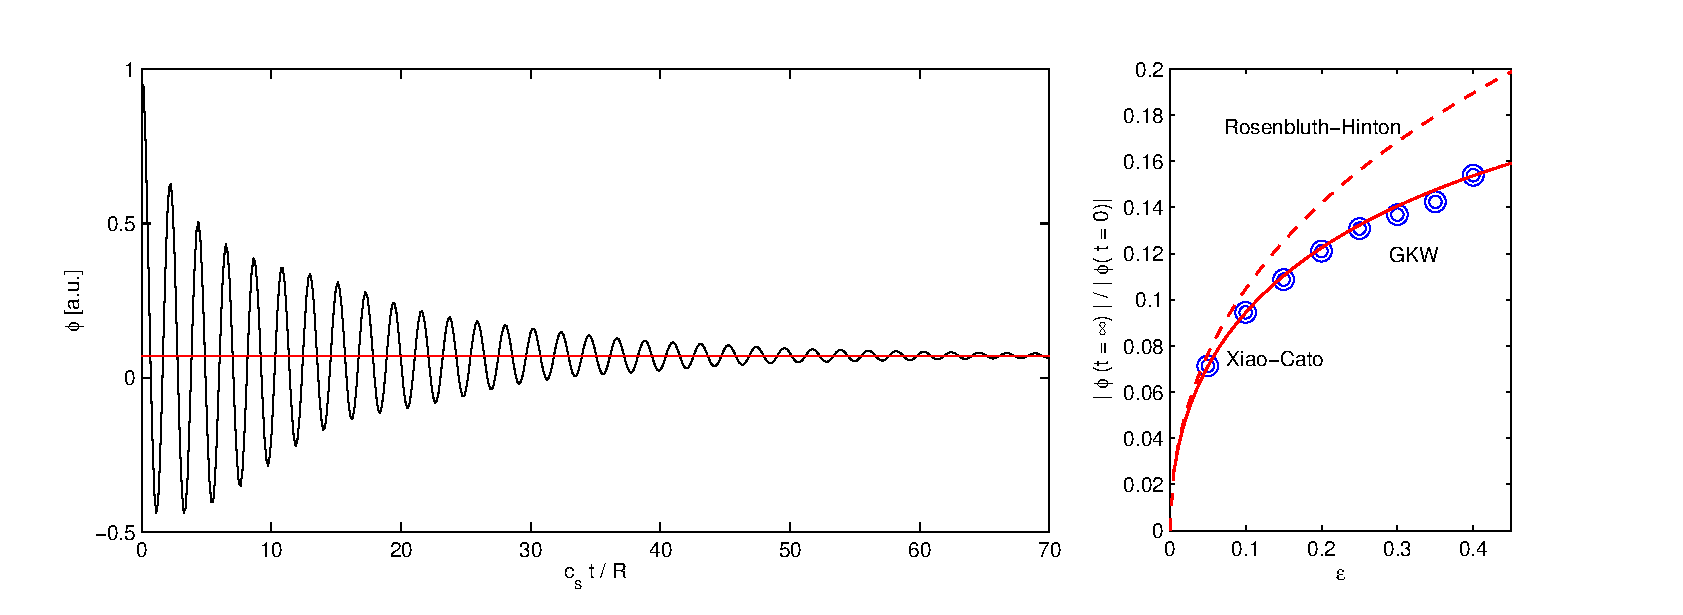
\includegraphics[width=14truecm]{RHbench.eps}
\caption{Zonal flow benchmark. Left: The potential perturbation (normalised to the potential at 
$t = 0$) as a function of normalised time, for $q = 1.3$, $\epsilon = 0.05$. The horizontal line gives the 
residual (0.0711) as predicted in Ref.~\cite{XIA06}. For this value of $\epsilon$ a numerical residual 
of 0.0713 is obtained, i.e. in agreement with the analytic result to within 0.3 \%
Right: Residual $\phi (t = \infty) / \phi(0) $ as a function of $\epsilon$ for 
$q = 1.3$. The circles are the result of GKW, the dotted line is the Rosenbluth-Hinton result \cite{HINROS} and 
the full line gives the analytic result of Xiao-Catto \cite{XIA06}. \label{zonalfig}} 
\label{overall1}
\end{center}
\end{figure}  

The Cyclone base case with adiabatic electrons does not check the correct implementation of the 
kinetic electron response, and in general is not very sensitive to the effects associated with trapped 
particles. 
The physics effects associated with kinetic electrons can be well benchmarked by considering a Trapped Electron 
Mode. A benchmark with GS2 is shown on the left of Fig.~\ref{overall2}. The parameters are 
taken from a discharge in the ASDEX Upgrade tokamak \cite{PEE05}: $\hat s = 1.07$, 
$q = 1.57$, $\epsilon = 0.177$, $T_e / T_i = 3$, $R/L_{Ti} = 0$, electro-static, collisionless, 
and with an ion to electron mass ratio of a Deuterium plasma. 
The values of the density gradient as well as the temperature gradient are scanned. 
The agreement for the growth rates is good.  

\begin{figure}[htb] 
\begin{center}
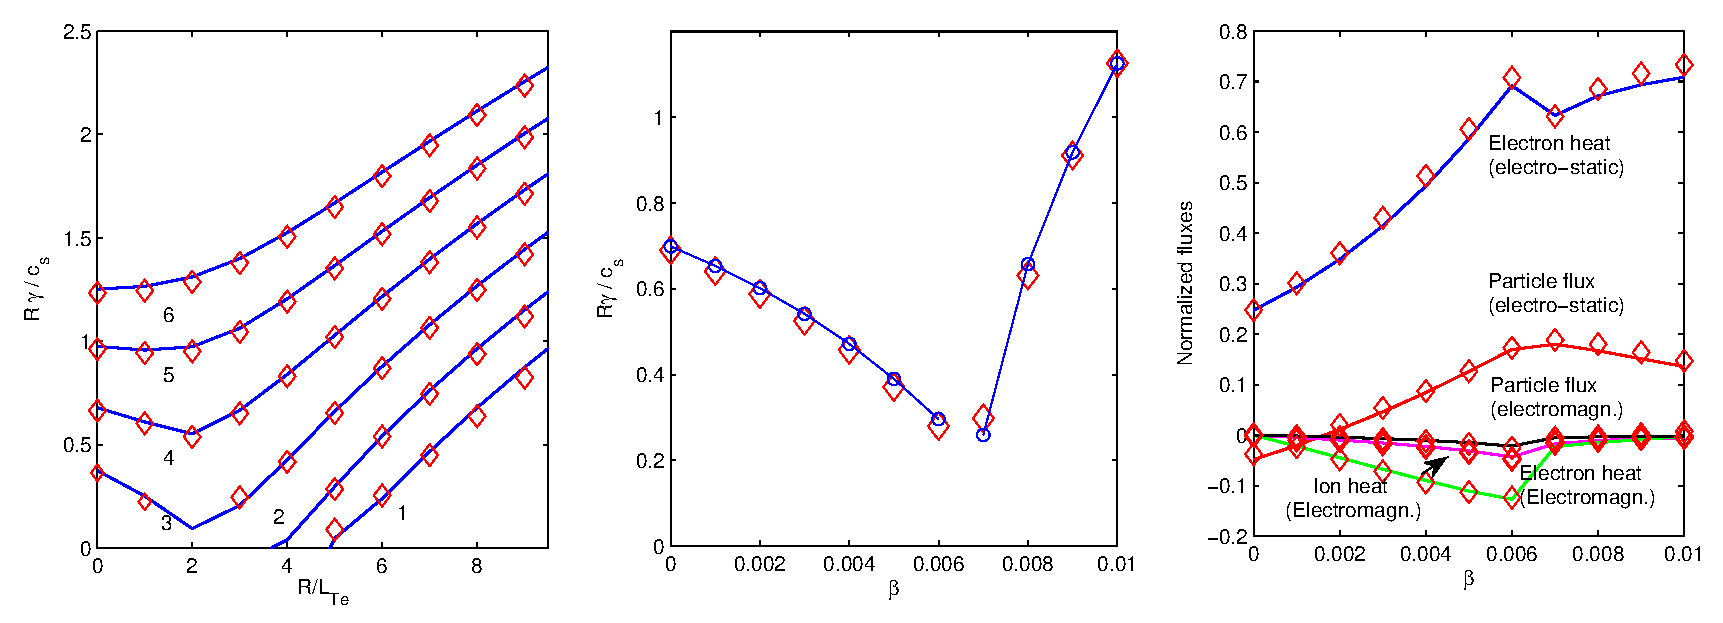
\includegraphics[width=16truecm]{overallfig-bench.eps}
\caption{Left: Benchmark of a trapped electron mode case. Shown is the normalised growth 
rate $R \gamma / c_s$ as a function of $R/L_{Te}$ for various values of $R/L_n$ indicated in 
the figure. Blue lines are the results of GS2 while red diamonds give the results of GKW. 
Middle: A benchmark of the growth rates of the ITG / Kinetic ballooning mode versus the plasma beta. 
Blue lines and circles 
are results from GS2 while red diamonds give the results of GKW. Right: The fluxes, normalised
to the ion heat flux as a function of beta. Lines give the results of GS2, while the diamonds give
the results of GKW.} 
\label{overall2}
\end{center}
\end{figure}  

Finite beta effects are tested for an ITG case increasing the plasma beta. The middle panel of 
Fig. \ref{overall2} shows the normalised growth rate as a function of the electron beta $\beta = n_e T_e 
/ (B^2 / 2 \mu_0)$ for the Waltz standard case $R/L_{Ti} = R/ L_{Te} = 9$, $R/ L_n = 3$, $q = 2$
$\hat s = 1$, $\epsilon = 0.166$ $T_e/T_i = 1$, and with a mass ratio of a Deuterium plasma. The ITG is 
stabilised by the finite beta effects and, at sufficient high values of beta, a kinetic ballooning 
mode is destabilised. The agreement for the growth rate between GKW and GS2 is again good. 
The electro-magnetic case also provides for a good benchmark of the calculation of the fluxes, since 
all fluxes (also the ones due to the magnetic flutter) are nonzero in this case. The right panel of 
Fig.~\ref{overall2} shows the comparison of the fluxes calculated by GS2 and GKW. Since for 
a linear problem the amplitude of the mode and, therefore, the magnitude of the fluxes is arbitrary, 
all fluxes have been normalised to the ion heat flux. This allows for a straightforward comparison 
between the codes. All calculated fluxes are again in good agreement. 

Effects of magnetic field compression are also tested with the linear Waltz standard test case $R/L_{Ti} = R/ L_{Te} = 9$, $R/ L_n = 3$, $q = 2$, $\hat s = 1$, $\epsilon = 0.166$, $T_e/T_i = 1$, the mode with the fastest electrostatic growth rate has been used: $k_{\perp} \rho_s = 0.3$. Fig. \ref{bpar-bm} shows that the ITG mode is hardly affected by the perturbation $B_{1 \parallel}$ but the kinetic ballooning mode is further destabilised with increasing $\beta$. Both with the growth rates and the parallel structure a good agreement with GS2 has been obtained.

\begin{figure}[htb] 
\begin{center}
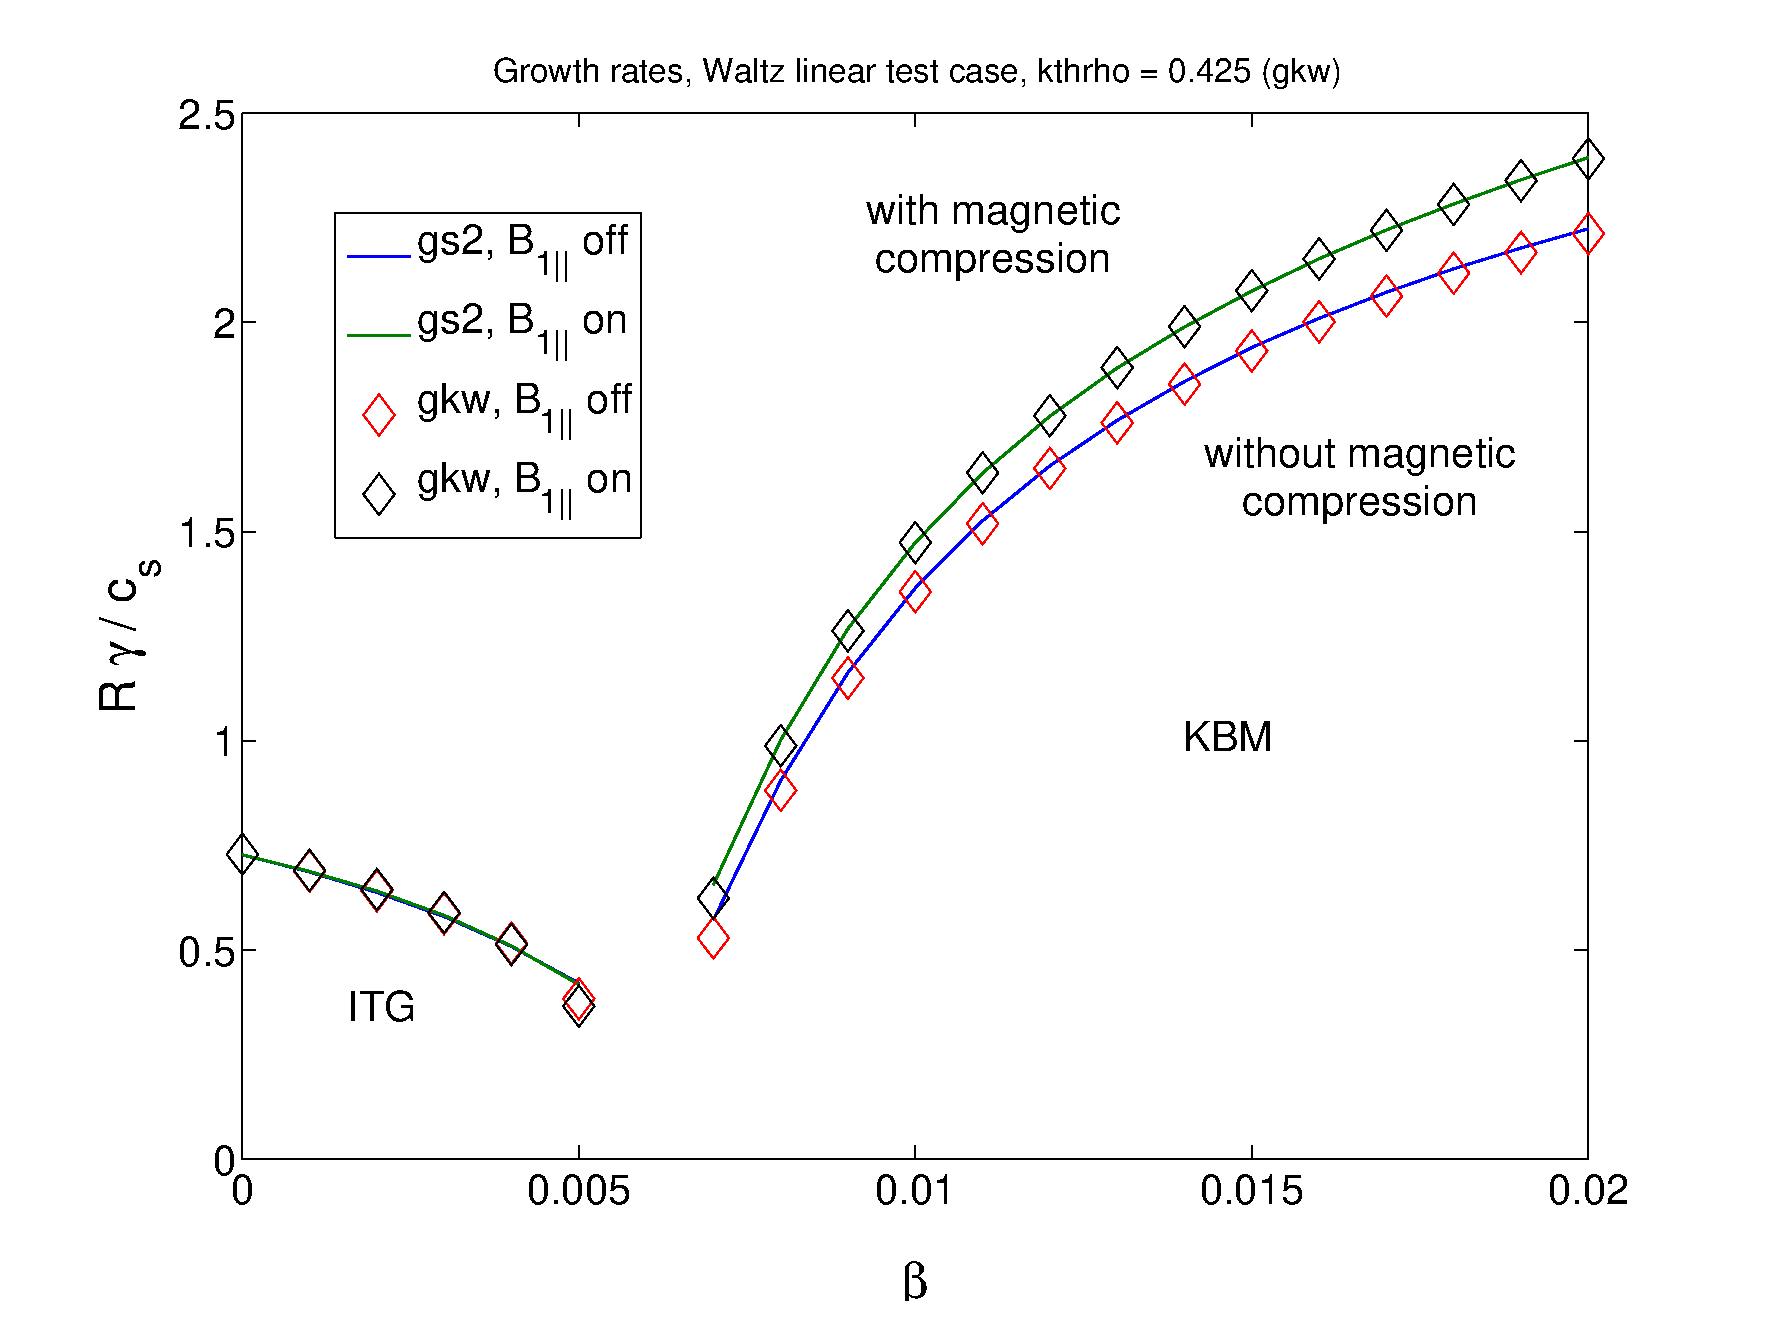
\includegraphics[scale=0.25]{bpar-growthrates-waltz-linear.eps}
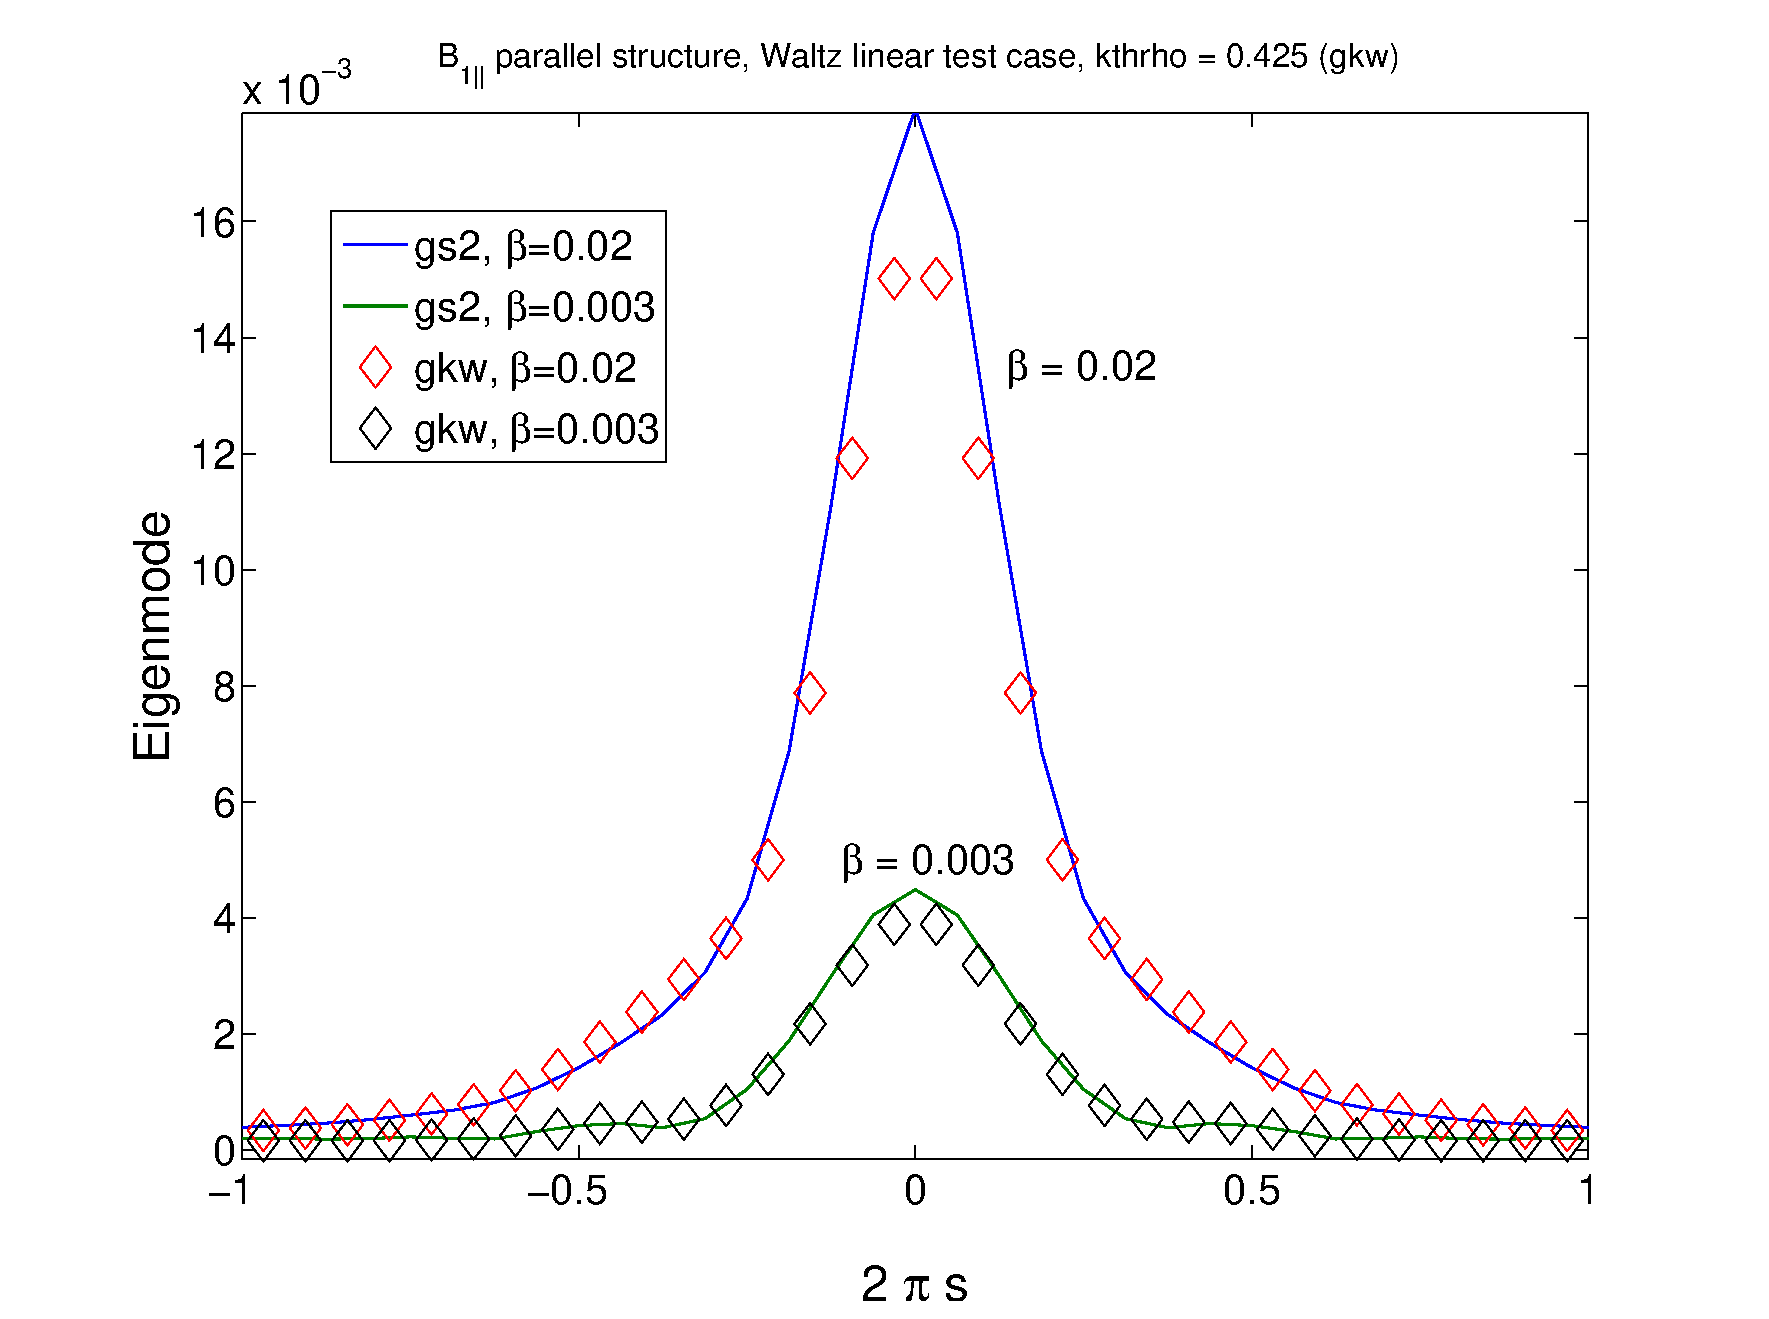
\includegraphics[scale=0.25]{bpar-parallelstructure-waltz-linear.eps}
\caption{Waltz linear test case. Left: Benchmark of growth rates of ITG and kinetic ballooning modes with magnetic field compression on and off. Right: Parallel structure of $B_{1 \parallel}$ in ITG and KBM regimes.} 
\label{bpar-bm}
\end{center}
\end{figure}

A collisionality benchmark of the pitch angle scattering against GS2 for a TEM is presented in Fig.~\ref{colls-tem}.  
To isolate the effect of e-e collisions and e-i collisions, the collisions input
variable $Z_{\rm eff}$
(a multiplier for the e-i collision rate) was varied.  Scattering of ions (off either species) made no difference for this benchmark 
(turning them on / off did not change the result of either code). This result was obtained with the Arakawa scheme and zero dissipation in $v_\parallel$. At low collisionalities, GKW convergence for a TEM requires many $v_\parallel$ points (the 64 used for this benchmark are not quite sufficient). 

\begin{figure}[htb] 
\begin{center}
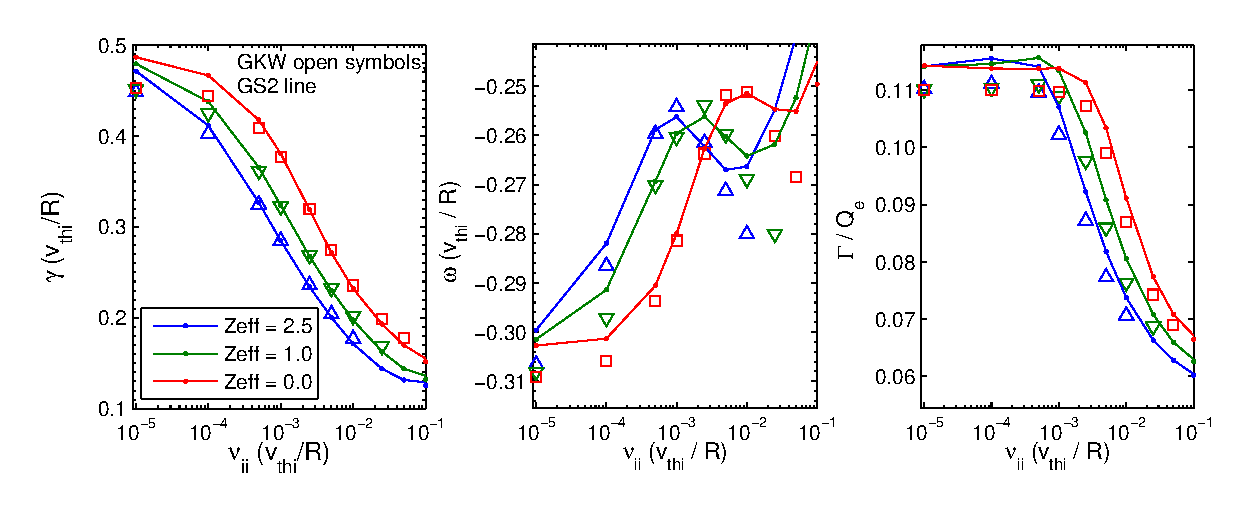
\includegraphics[scale=0.8]{bench-ee-sa-all.eps}
\caption{Collisions benchmark (pitch angle scattering) for a TEM with varying
$Z_{\rm eff}$} 
\label{colls-tem}
\end{center}
\end{figure}

The pitch angle collisions have also been benchmarked against GS2 in Ref.~\cite{PEE09scmode}, with good agreement 
obtained for the particle flux as a function of collisionality. 
The treatment of arbitrary toroidal geometry has been benchmarked against GS2 by performing an elongation scan. The parameters considered are $R/L_{Ti} = R/ L_{Te} = 8.9$, $R/ L_n = 2.85$, $q = 1.42$ $\hat s = 1.25$, $\epsilon = 0.182$, $T_e/T_i =1$ for deuterium ions and adiabatic electrons. 
The elongation of the last closed flux surface is varied from $\kappa=1.2$ to $\kappa=1.6$ and the corresponding MHD equilibrium is calculated using the CHEASE code \cite{LUT96}.
This equilibrium is then used for the calculation of the metric tensors both in GKW and GS2. 
The results for the linear growth rate as a function of $k_\theta\rho_s$ are shown in Fig.~\ref{geom-bench} showing a good agreement between the two codes.  The wavevector
normalisation (projection) in the two codes in general differs (GKW uses
$g^{\zeta\zeta}(LFS)$ while GS2 uses ${\cal E}^{\psi\zeta}$ \cite{dorland-note} which are only equivalent in `$s-\alpha$' geometry) and must
be corrected for (in this case the GKW $k_\theta$ inputs were rescaled). 
Note that the results are significantly different from the ones obtained with the simplified `$s-\alpha$' equilibrium shown by 
the dashed line (obtained with GKW).
\begin{figure}[htb] 
\begin{center}
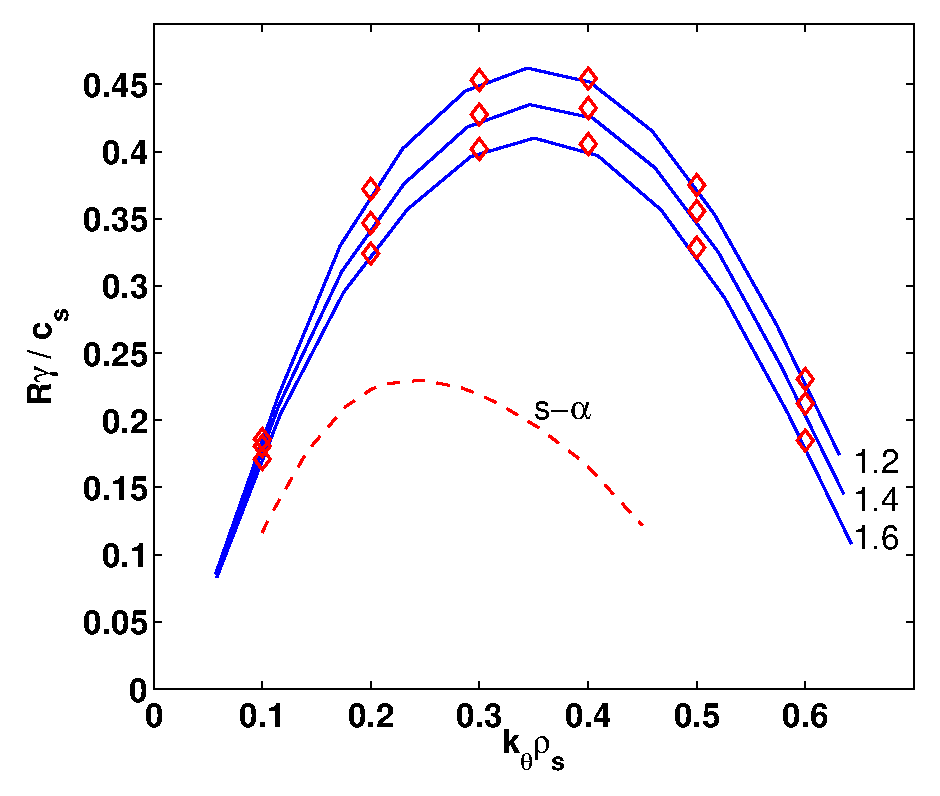
\includegraphics[width=6truecm]{geom-bench.eps}
\caption{Benchmark of the geometry treatment. The normalised growth 
rate $R \gamma / c_s$ is shown as a function of GS2 $k_\theta\rho_s$ for various values of the last closed flux surface elongation $\kappa$ indicated in 
the figure. Blue lines are the results of GS2 while red diamonds give the results of GKW. The results
obtained for the simplified `$s-\alpha$' equilibrium
with GKW are indicated by the red dashed line.} 
\label{geom-bench}
\end{center}
\end{figure}  

The effects of impurities have been benchmarked against GS2 using again the Waltz standard test case with
`$s-\alpha$' geometry $R/L_{Ti} = R/ L_{Te} = 9$, $R/ L_n = 3$, $q = 2$, $\hat s = 1$, $\epsilon = 0.166$, $T_e/T_i = 1$. Collisions were not included in this test. The left panel of Fig. \ref{impurities} shows the ITG-TEM part of the linear electro-static growth rate spectra for 4 different lithium impurity concentration. The increasing impurity density was balanced by lowering the amount of deuterium in order the preserve quasi-neutrality. This means that the increasing $n_{Li}$ leads to larger values of $Z_{\mathrm{eff}}$ which is accountable for the stabilisation of the TEM modes. 

On the middle panel of Fig. \ref{impurities} the effect of varying the type of the impurity species can be seen. The impurity density is kept at a constant 1\% in this test. Fully ionized lithium, carbon and neon and partially ionized (charge number Z=10 for both cases) iron and tungsten ions have been used. Quasi-neutrality was maintained by adjusting the deuterium density. Here, as well, the increasing $Z_{eff}$ has a stabilizing effect on the TEM modes.

And finally, the right panel of Fig. \ref{impurities} shows the effect of the two electro-magnetic perturbations, the magnetic flutter $A_{\parallel}$ and the magnetic compression $B_{\parallel}$, obtained with a lithium impurity density of 10\%. The growth rates are significantly increased compared to the electro-static cases. Apart from the longest wavelength modes a good agreement is found between the two codes. 

\begin{figure}[htb]
\begin{center}
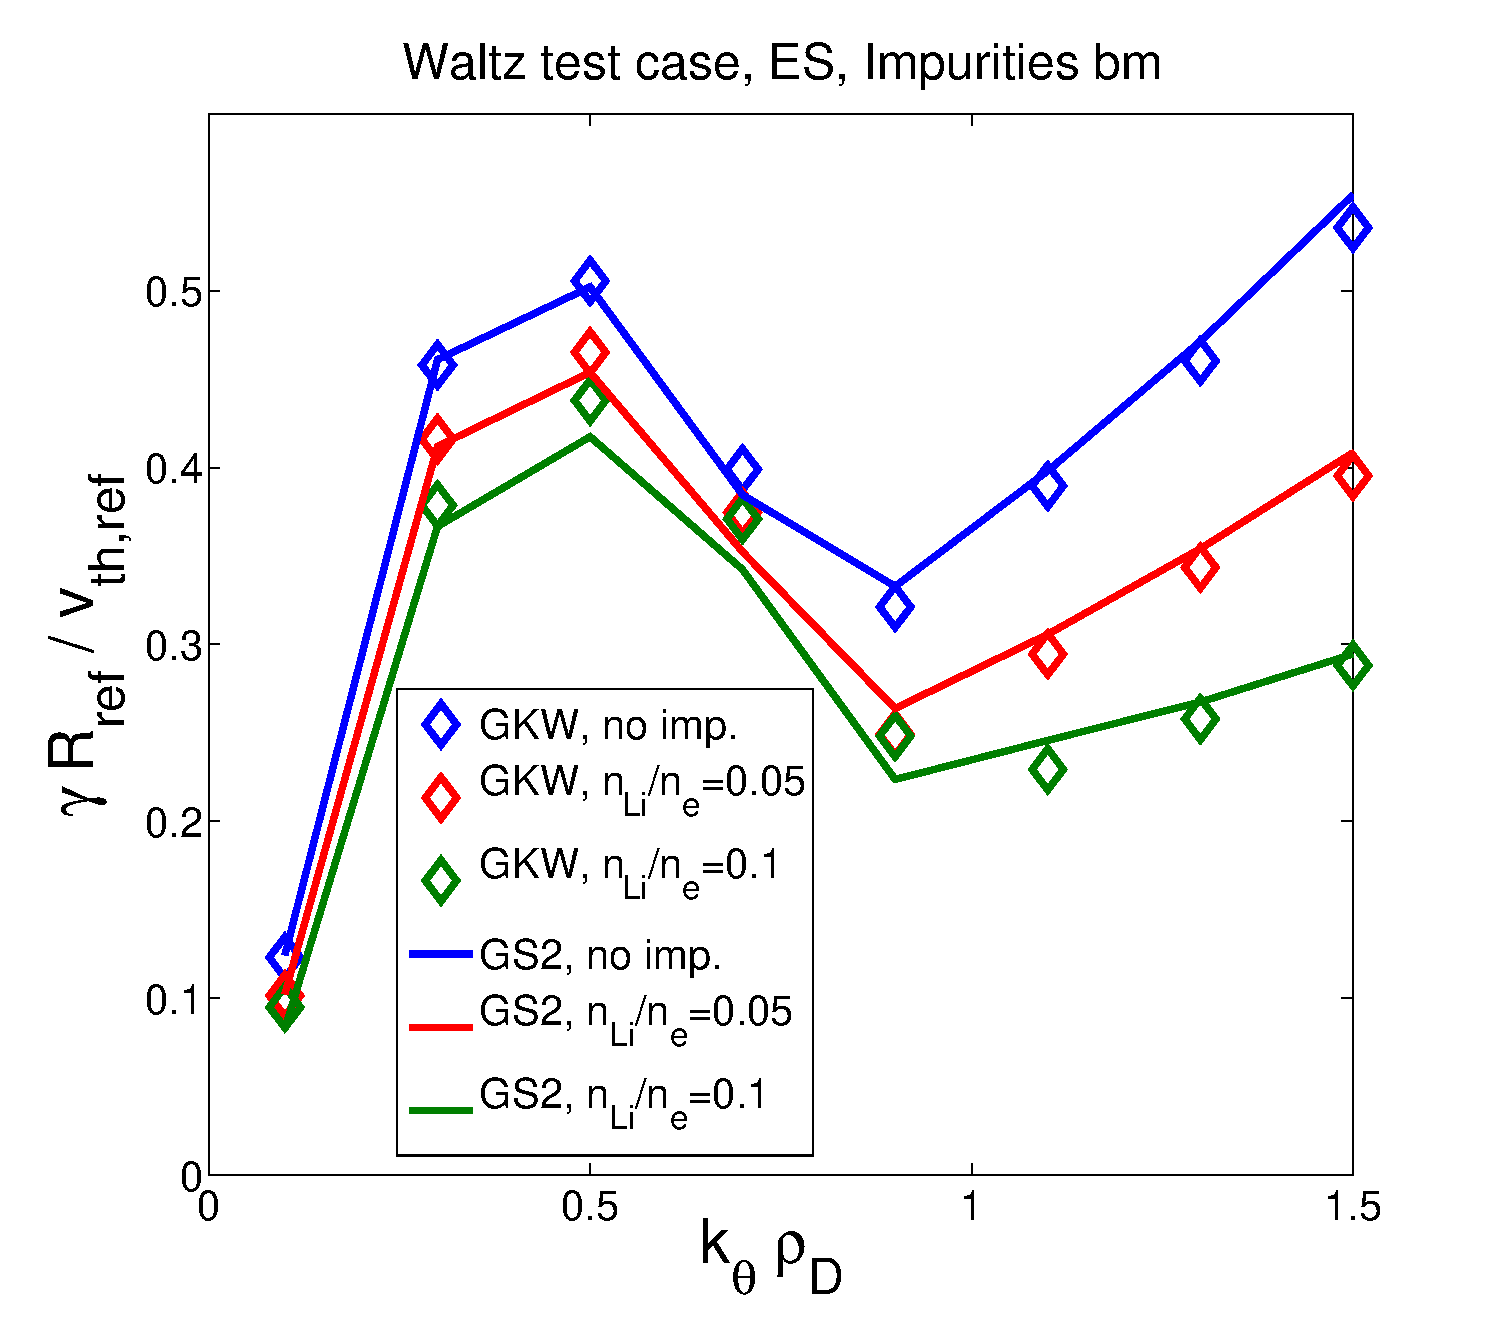
\includegraphics[scale=0.21]{waltz-gr-es-sa-nocoll.eps}
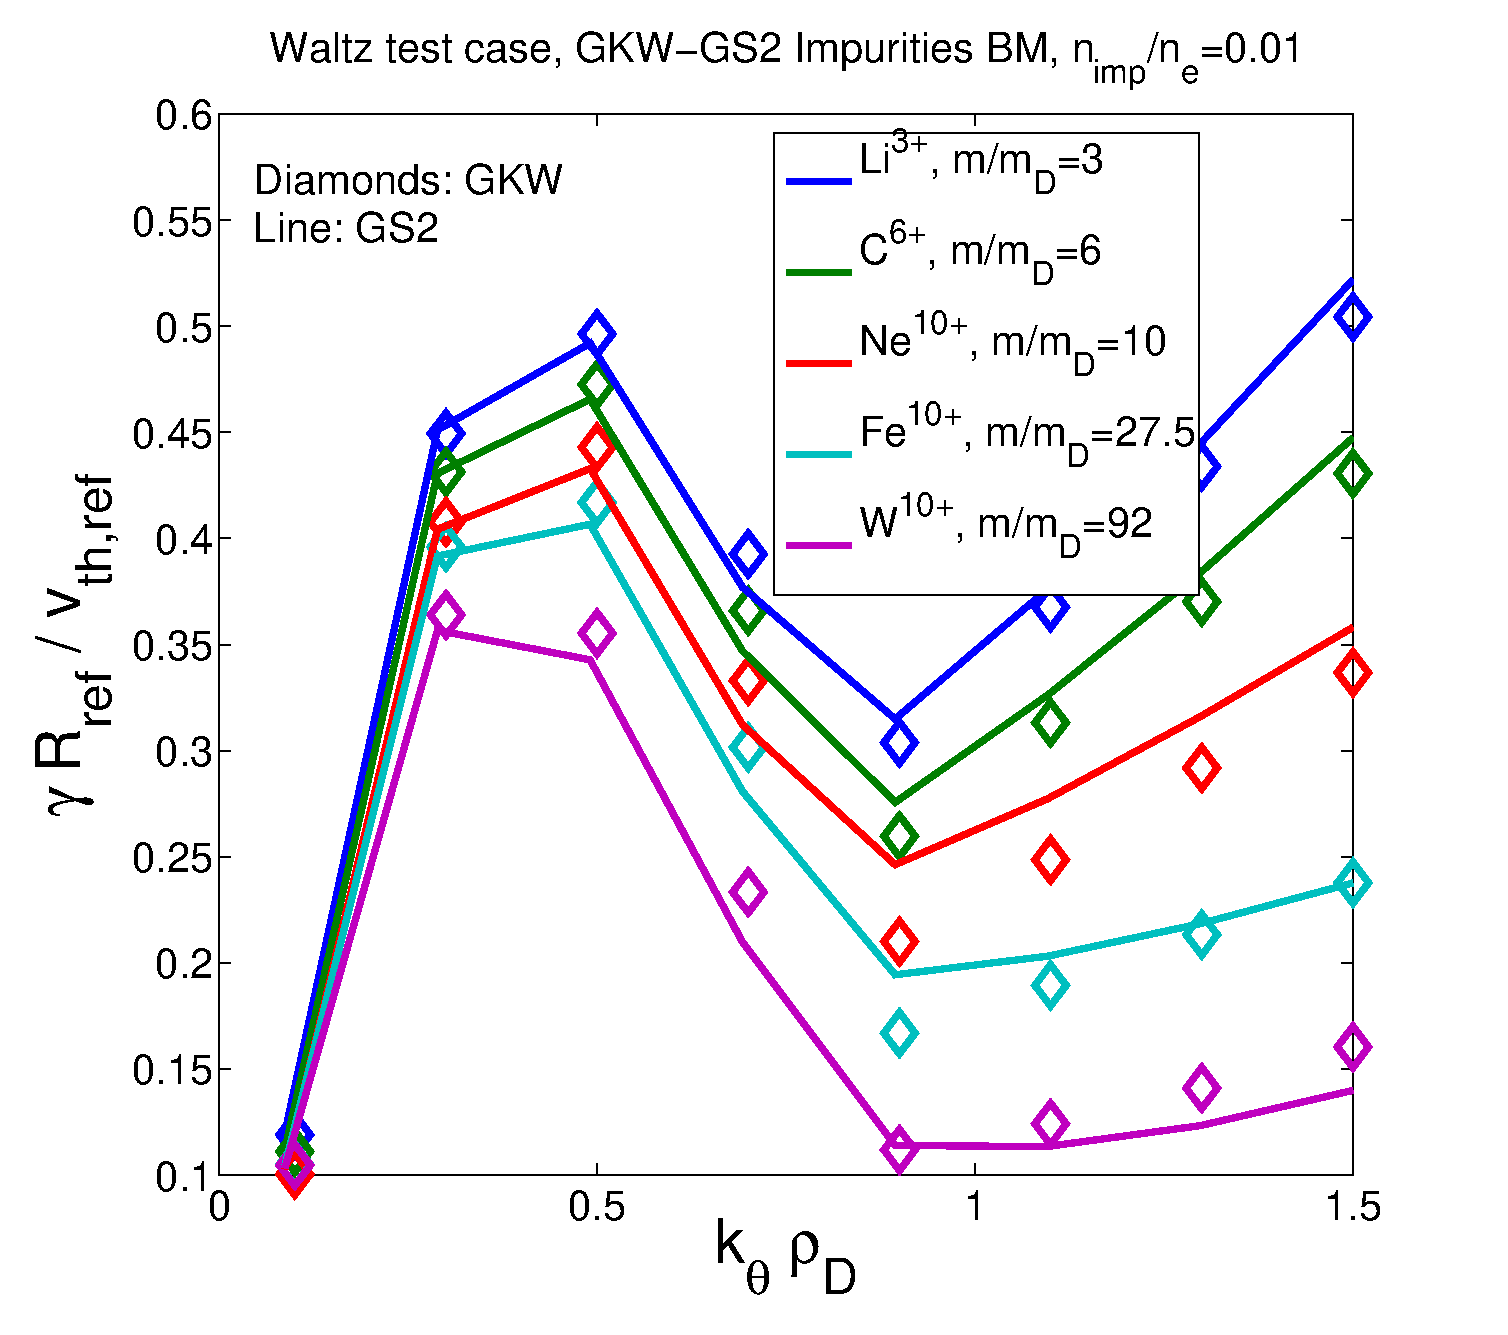
\includegraphics[scale=0.21]{waltz-gr-es-sa-Zimp-nocoll.eps}
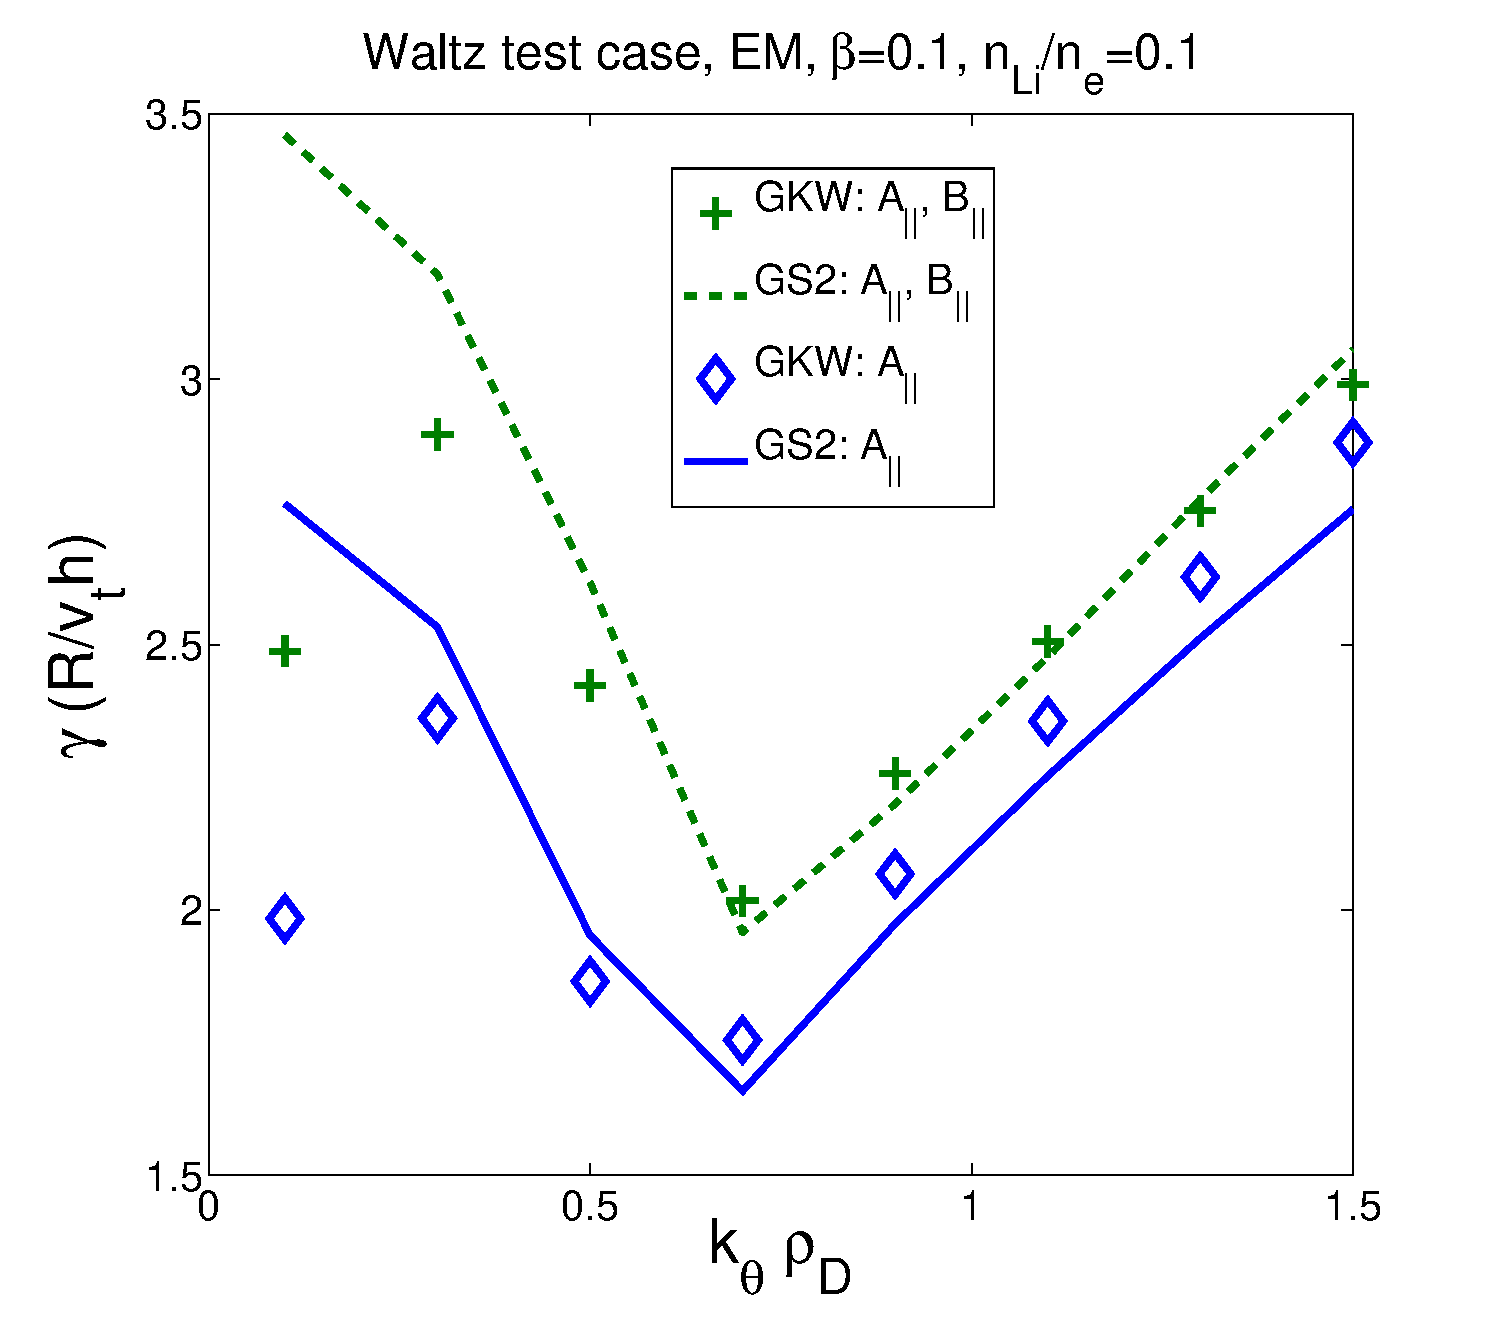
\includegraphics[scale=0.21]{waltz-gr-em-sa-nocoll.eps}
\caption{Benchmark of impurity treatment, growth rates of the Waltz standard test case with `$s-\alpha$' equilibrium without collisions. Line: GS2, diamonds: GKW. Left panel: effect of varying the Li impurity concentration, electro-static. Middle panel: effect of changing the impurity species, electro-static. Right panel: effect of the electro-magnetic perturations. Green line: fully electro-magnetic, both $A_{\parallel}$ (magnetic flutter) and $B_{\parallel}$ (magnetic compression) are retained. Blue line: only $A_{\parallel}$ is included.}
\label{impurities}
\end{center}
\end{figure}

The Miller geometry has been benchmarked against GS2, also for the adiabatic Waltz Standard case, with $\epsilon$ changed to 0.266.  As for the general geometry benchmark, the
different wavevector normalisations must be corrected (in this case the GS2 $k_\theta$ inputs were rescaled), after which very good agreement is found (Fig. \ref{miller}.).  The squareness and elevation have not been
benchmarked since GS2 does not have these parameters.  Some of the Miller parameters are defined differently in the two codes and require a simple conversion.

\begin{figure}[htb]
\begin{center}
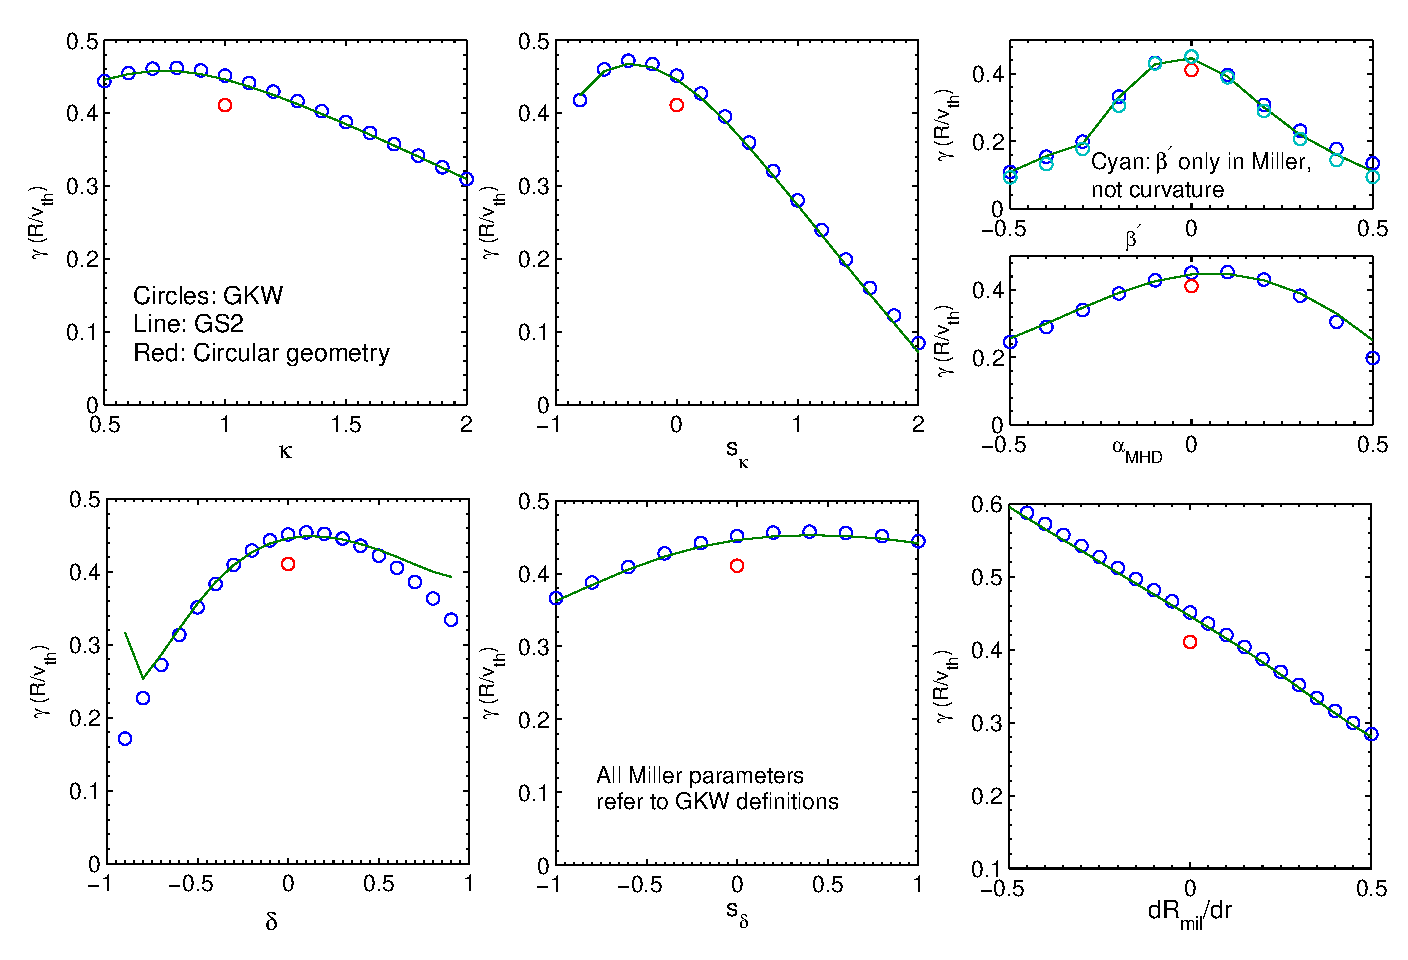
\includegraphics[scale=0.65]{geom-miller.eps}
\caption{Benchmark of the Miller geometry for the growth rates of the adiabatic
Waltz standard case with $\epsilon=0.266$ and GKW $k_\theta \rho_i=0.43$. Line: GS2, Circles: GKW.  The Miller
parameters shown on the horizontal axes refer to the GKW definitions.}
\label{miller}
\end{center}
\end{figure}


\section{Nonlinear benchmarks} 

\begin{figure}[thb] 
\begin{center}
\includegraphics[width=12 truecm,clip]{heatflux.eps}
\caption{GKW results of the electron heat flux expressed as a heat conduction coefficient (normalised
to $\rho_e^2  c_e / L_T$ with $c_e = \sqrt{T_e/m_e}$) as a function of normalised time ($t_{NN} = tc_e/L_T$)
for the Nevins ETG benchmark}
\label{cyclone-nl} 
\end{center}
\end{figure} 

For the nonlinear solution there are two well established benchmark cases for which several codes have 
been compared: the cyclone base case, and the Nevins ETG benchmark. 
GKW has been benchmarked against the European gyrokinetic codes for the Cyclone case 
in Ref.~\cite{Euro-bench}. 

Here we  describe the alternative ETG benchmark of Nevins \cite{NEV08}. The 
parameters for this case are the same as those of the Cyclone base case ($R/L_T = 6.9$, 
$R/L_n = 2.2$, $q = 1.4$, $T_e / T_i = 1$, $\epsilon = 0.18$) with only the magnetic shear 
changed to $\hat s = 0.1$. For this case the electron dynamics is simulated while the 
ions are assumed adiabatic. The latter response does not include the flux surface average 
of the electro-static potential, i.e. the response is proportional to $n_i \phi / T_i$.  
To obtain the same results as published in Ref.~\cite{NEV08} we have used (and must use)
the same number of bi-normal modes $N_{\rm mod} = 8$, and mode spacing $(k_\perp \rho_s)_{\rm max} 
= 0.69$. The radial grid spacing is $\Delta (k_r \rho_s) =0.0619$ with $N_x = 41$ (both 
positive and negative wave vectors counted).  Finally, $N_\mu = 8$, $N_{v_\parallel} = 
16$, and $N_s = 16$. 

\begin{figure}[thb] 
\begin{center}
\includegraphics[width=12truecm]{shear-scan3.eps}
\caption{GKW results of the electron heat conduction coefficient for different values
of the magnetic shear}
\label{cyclone-nl2} 
\end{center}
\end{figure}  

Figure~\ref{cyclone-nl} shows the normalised electron heat flux as a function of the normalised
time. Averaging over the time interval ($1000 < t c_e / L_T < 19500$), 
GKW predicts a heat diffusion coefficient $\chi_e = 3.08 \pm 0.19$ in good agreement with the 
value $\chi_e = 2.95\pm 0.15$ reported in Ref. \cite{NEV08}. The ETG case is 
sensitive to the magnetic shear. For values $\hat s > 0.3$ no convergence is found in the simulations 
reported in Ref. \cite{NEV08}. GKW reproduces this result as shown in Fig. \ref{cyclone-nl2}.

\begin{figure}[htb] 
\begin{center}
\subfigure[Benchmark with GYRO]{\includegraphics[height=145pt]{exb-benchmark}}
\subfigure[Benchmark with GS2]{\includegraphics[height=150pt]{GKW-GS2-exb}}
\caption{Left: GKW benchmark of background ExB shearing with GYRO for Waltz standard case parameters. GKW results (diamonds) for
 adiabatic electrons, kinetic electrons, and adiabatic with $\hat s = -0.5$, are compared to the equivalent GYRO results (circles) from Tables II, III, IV and V  of Ref. \cite{KIN05}. The dashed lines include coupled
parallel velocity shear for purely toroidal rotation with $u^\prime=12\gamma_E$.  Right: GKW benchmark of background ExB shearing with GS2 results reported in Ref. \cite{ROA09} for Cyclone case parameters.  Both codes were run including coupled parallel velocity shear for purely toroidal rotation.  $\gamma_{\rm max}$ is the maximum linear growth rate at $\gamma_E=0$.}
\label{exb-gyro} 
\end{center}
\end{figure} 

The background ExB shear stabilisation 
has been successfully benchmarked against GYRO results as reported in Ref. \cite{CAS09}.  This result for the Waltz standard case 
is included again here for convenience in Fig. \ref{exb-gyro}.  GKW has also been checked against 
the GS2 results reported in Ref. \cite{ROA09} for the Cyclone case, also shown in Fig. \ref{exb-gyro}.  Both of these comparisions were against existing results, i.e. no further attempt to examine the convergence of the GYRO and GS2 results has been made.  Detailed convergence testing for the GKW results is described in Refs. \cite{Casson-Thesis} and \cite{exb-dissip}.  This study revealed that it is preferable to use some radial hyperdissipation and minimal parallel dissipation at high shear rates (see also Sec. \ref{sec.dissip}.) (not the case for these figures) which can improve the agreement at high shear rates to better than that shown in Fig. \ref{exb-gyro}.

Towards the edge, nonlinear and electromagnetic physics can be significantly more complex than
the ITG dominated Cyclone and GA-STD cases,
and benchmarking in this area is an active area of research.  
For L-mode ASDEX-Upgrade plasmas, GKW has been sucessfully benchmarked with GENE 
for four nonlinear electromagnetic cases using full geometry, and full collisions.  The results 
are reported in in Refs. \cite{FAB13} and \cite{TOL13}.  
Benchmarking for the the DIII-D `shortfall' case is in progress and 
is reported in ITPA presentations of C. Holland and Y. Camenen.

\subsection{Global Benchmarks}

Can be found in the Ringberg 2012 presentation of A.G Peeters on the GKW webpages under Talks..


\vskip 0.2 truecm

\noindent{\bf Acknowledgements} The authors want to thank W. Dorland and M. Kotschenreuther 
for making the GS2 code available, as well as A. Marinoni for his contribution to the geometry benchmark.
One of the authors (AGP) would also like to thank Bruce D. Scott for 
his tutorials and insights into the subject which he has been able to follow over many years.

% related to auctex mode and latex-preview-mode in Emacs:
%%% Local Variables:
%%% mode: latex
%%% TeX-master: "doc"
%%% End:

%\fancyfoot[L]{$ $Date$ $}
%\fancyfoot[R]{$ $Revision$ $}

\chapter{Neoclassical background}

By default the background distribution function in considered to be a Maxwellian.  However due to background flows the temperature and density 
gradients, coupled with the geometry and collisions, the distribution function can deviate from the Maxwellian by a small amount.   This section describes the implementation of the interface between NEO and GKW so that small deviations from background Maxwellian can be included.

\section{Form of the equations for arbitrary background}

The corrections to the background Maxwellian are calculated, at the moment, by the Eulerian
Neoclassical transport code {\small NEO} \cite{NEO1,NEO2}.  

We start with the gyro-kinetic Vlasov equation in (${\bf X}, v_\parallel, 
\mu$) coordinates,
\begin{equation}
{\partial f_{\rm tot} \over \partial t} + {{\rm d} {\bf X} \over {\rm d} t} \cdot \nabla_\mu 
f_{\rm tot} + {{\rm d} v_\parallel \over {\rm d} t} {\partial f_{\rm tot} \over \partial v_\parallel} = 0 .
\label{eq:neoclassics-vlasov}
\end{equation}

Finally
\begin{eqnarray}
\frac{\partial f}{\partial t} + \underbrace{v_{||}{\bf b}\cdot\nabla f}_{I} + \underbrace{{\bf v}_D\cdot\nabla f}_{II} + \underbrace{{\bf v}_\chi \cdot\nabla f}_{III} - \underbrace{\frac{{\bf b}}{m}\cdot (\mu\nabla B + \nabla\epsilon_\Omega)\frac{\partial f}{\partial v_{||}}}_{IV} = \\
-v_{||}{\bf b}\cdot\nabla F_{0} -\underbrace{({\bf v}_D + {\bf v}_\chi)\cdot\nabla F_{0}}_{VI + V} + \underbrace{\frac{Ze}{mv_{||}}(v_{||}{\bf b} + {\bf v}_D)\cdot\nabla\phi \frac{\partial F_{0}}{\partial v_{||}}}_{VII + VIII} + \frac{({\bf v}_D + {\bf v}_\chi)}{mv_{||}}\cdot\mu\nabla B\frac{\partial F_{0}}{\partial v_{||}} + C(f)
\end{eqnarray}
Where the first term on the right hand side and Term VI are the terms in the drift-kinetic equation that is solved by NEO:
\begin{equation}
{\bf v_{D}}\cdot\nabla F_{0}+ v_{||}{\bf b}\cdot\nabla F_{0} -\frac{\mu}{m}{\bf b}\cdot\nabla B\frac{\partial F_{0}}{\partial v_{||}}= C(F_{0}).
\end{equation}
This equation determines the form of the perturbation to the background distribution function.

The background distribution function is split into two stationary components, $F_0 = F_{M} + F_{\mbox{neo}}$, the first term is a lowest order Maxwellian and the second is its neoclassical correction.  The Maxwellian distribution function and its derivatives have the form:

\begin{eqnarray}
F_{M} = \frac{n_{0}}{\pi^{3/2}v_{th i}^{3}}\exp{\left(-\frac{(v_{||}-RB_{t}\omega_{\phi}/B)^{2} + 2\mu B/m}{v_{th i}^{2}}\right)}\\
\nabla F_{M} = \nabla P F_{M} - \frac{\mu\nabla B}{T}F_{M} \\
\partial F_{M}/\partial v_{||} = -\frac{mv_{||}}{T}F_{M} \\
\nabla P = \frac{\nabla n}{n} + \left(\frac{v_{||}^{2}}{v_{th}^{2}} + \frac{\mu B}{T} - \frac{3}{2}\right)\frac{\nabla T}{T} - \frac{mv_{||}}{T}\frac{RB_{t}}{B}\nabla\omega_{\phi} \nonumber\\
\end{eqnarray}
where Eq.17 is the Maxwellian derivative considering only the thermodynamic quantities, the gradient in the magnetic field we leave separate.  Derivatives of the perturbed background are taken numerically using fourth order central differencing.  There is a subtlety in the equations where, when considering a Maxwellian background the gradient in the magnetic field terms cancel 
exactly with the trapping force term acting on the Maxwellian. 
The background Maxwellian has only a radial derivative and $\omega_{\phi}$ is the angular toroidal rotation frequency.

The source term for the Maxwellian component of the background for each species, $s$, ($S(F_{0}) = S(F_{M,s})+S(F_{\mbox{neo},s})$) is given by:

\begin{eqnarray}
S(F_{M,s}) = -\frac{1}{Z_{s}eB}\left(\frac{mv_{||}^{2}}{B}+\mu\right)\left(\frac{{\bf b}\times\nabla B}{B}\right)\cdot F_{M,s}\nabla P -\left(\frac{{\bf b}\times\nabla \phi}{B}\right)\cdot F_{M,s}\nabla P \nonumber\\
-\frac{v_{||}Ze}{T_{s}}{\bf b}\cdot\nabla\phi F_{M,s} -\frac{1}{T}\left(\frac{mv_{||}^{2}}{B}+\mu\right){\bf b}\cdot\frac{\nabla B\times\nabla\phi}{B}F_{M,s}.
\end{eqnarray}
 
Terms involving gradients of the magnetic field, $\mu\nabla B$  cancel out, leaving only terms involving $\nabla P$.  In contrast, for the neoclassical correction this cancellation does not occur, the source term has the form,

\begin{eqnarray}
S(F_{\mbox{neo}},s) = -\frac{1}{Z_{s}eB}\left(\frac{mv_{||}^{2}}{B}+\mu\right)\left(\frac{{\bf b}\times\nabla B}{B}\right)\cdot \nabla F_{\mbox{neo},s} -\left(\frac{{\bf b}\times\nabla \phi}{B}\right)\cdot\nabla F_{\mbox{neo},s}+ \nonumber\\ \frac{Z_{s}e}{m}{\bf b}\cdot\nabla\phi \frac{\partial F_{\mbox{neo},s}}{\partial v_{||}} + \frac{1}{mv_{||}}\left(\frac{mv_{||}^{2}}{B}\right){\bf b}\cdot\frac{\nabla B\times\nabla\phi}{B} \frac{\partial F_{\mbox{neo},s}}{\partial v_{||}}.
\end{eqnarray}

\section{Equation modifications}

For the sake of completeness and to document exactly
which equations are being solved, the modifications to the equations in the electrostatic limit are written here.
The equations, as in the previous sections, can be written in the form 
\begin{equation}
\label{eqs:neoclassics-complete-set}
{\partial f \over \partial t} = {\rm III} + {\rm IV} + {\rm V} + {\rm VII}+ {\rm VIII}.
\end{equation}
Only terms that are modified by the
neoclassical background are described here, then each term is, in its normalised form:

\begin{eqnarray}
{\rm III} &\rightharpoonup& - {\bf v}_\chi \cdot \nabla f =  \frac{{\bf b}\times\nabla\phi}{B}\cdot\nabla{f} \rightarrow 
\imath k_{\zeta}\varepsilon^{\psi\zeta} \frac{\partial\phi_{\mbox{neo}}}{\partial\psi} f + \imath k_{\zeta}\varepsilon^{s\zeta} \frac{\partial\phi_{\mbox{neo}}}{\partial s} f + \imath k_{\psi}\varepsilon^{s\psi} \frac{\partial\phi_{\mbox{neo}}}{\partial s} f \nonumber\\
\noalign{\vskip 0.6 truecm}
{\rm IV} &\rightharpoonup& -\frac{1}{mv_{||}}\left(v_{||}{\bf b}\cdot\left(\mu\nabla B + Ze\nabla\phi\right)\right)\frac{\partial f}{\partial v_{||}} 
= -\frac{1}{m}\left({\bf b}\cdot\left(\mu\nabla B + Ze\nabla\phi_{\mbox{neo}}\right)\right)\frac{\partial f}{\partial v_{||}} \nonumber\\ &\rightarrow& -\left(\mu_{N}v_{s}\mathcal{F} \frac{\partial B_{N}}{\partial s} + \frac{v_{s}Z}{2T_{s}}\mathcal{F}\frac{\partial\phi_{\mbox{neo},N}}{\partial s}\right)\frac{\partial f}{\partial v_{|| N}}\nonumber\\
\noalign{\vskip 0.6 truecm}
{\rm V} &\rightharpoonup& - {\bf v}_\chi \cdot \nabla F_0 =\frac{{\bf b}\times\nabla x^{\alpha}}{B}\imath k_{\alpha}\phi\cdot\nabla F_0 \rightarrow
\varepsilon^{\alpha\psi}\imath \rho_{i}k_{\alpha}\cdot\nabla\psi_{N} \frac{\partial F_{M}}{\partial\psi}\phi_{N} + \imath\varepsilon^{\alpha\beta} \rho_{i}k_{\alpha}\phi_{N}\frac{\partial F_{\mbox{neo}}}{\partial x^{\beta}}\nonumber\\
\noalign{\vskip 0.6 truecm}
{\rm VII} &\rightharpoonup& \frac{Ze}{m_{s}} {\bf b}\cdot\nabla\phi \frac{\partial F}{\partial v_{||}}  \rightarrow -\frac{Zv_{s}}{T_{s}} v_{||N} \mathcal{F}\frac{\partial\phi_{N}}{\partial s} F_{M} + \frac{Zv_{s}}{2T_{s}} \mathcal{F}\frac{\partial\phi_{N}}{\partial s} \frac{\partial F_{\mbox{neo}}}{\partial v_{N||}} \nonumber\\
\noalign{\vskip 0.6 truecm}
{\rm VIII} &\rightharpoonup& -\frac{Ze}{v_{||}m_{s}} \vec{v_{D}}\cdot\nabla\phi \frac{\partial F}{\partial v_{||}} \rightarrow-i\frac{k_{\alpha}Z}{T_{s}}\vec{v_{D}}\cdot\nabla x^{\alpha}\phi_{N}F_{M}+\frac{\imath k_{\alpha}Z}{2T_{s}v_{||N}} \vec{v_{D}}\cdot\nabla x_{a}\phi_{N} \frac{\partial F_{\mbox{neo}}}{\partial v_{||N}}\nonumber\\
\end{eqnarray}

\section{The NEO code}

{\small NEO} outputs the neoclassical distribution function, $F_{NEO}$, and the neoclassical electrostatic 
potential, $\phi_{NEO}$.   To run {\small NEO} in a way that can be read by {\small GKW} the following input files are needed for  {\small NEO}:
\begin{itemize}
\item {\bf input.neo} - Input file
\item {\bf input.profiles} - The radial profiles of experimental data.  Needed for the normalisation of the velocities.
\end{itemize}
When run the following files must be in the folder that {\small GKW} runs in,
\begin{itemize}
\item {\bf out.neo.equil} - Equilibrium quantities per species
\item {\bf out.neo.f} - The distribution functions in spectral form
\item {\bf out.neo.grid} - The poloidal and radial grid sizes and points
\item {\bf out.neo.expnorm} - The normalising quantities
\end{itemize}
The latter file is only produced when {\small NEO} is run in profile mode which requires a relevant {\bf input.profiles} file.  Files for the Cyclone base case benchmark outlined in the next section can be found below and in the repository.

The neoclassical component of the background distribution function, $F_{\mbox{neo}}$ is calculated and output by {\small NEO}, which is then read into GKW and transformed from a harmonic expansion in velocity space into real velocity space as utilised by GKW.  In {\small NEO} the non-adiabatic part of the distribution function is represented by.
\begin{eqnarray}
G_{\mbox{neo},s} = F_{M,s}\sum_{l=0}^{N_\xi}\sum_{m=0}^{N_{E}}\hat{g}_{l,m}P_{l}(\xi)L^{k(l)+1/2}_{m}(v_{s}^{2}/v_{th}^{2})(v_{s}/v_{th})^{k(l)},\nonumber\\
\end{eqnarray}
where $P_{l}(\xi)$ are Legendre polynomials and $L_{m}^{\alpha}(v)$ are Laguerre polynomals and $\hat{g}_{l,m}$ are the amplitudes and is related to the distribution function, $F_{\mbox{neo},s}$ by, $F_{\mbox{neo},s}=G_{\mbox{neo,s}}-F_{Ms}\phi_{\mbox{neo}}e/T_{s}$.  As a benchmark of this process, Figure \ref{neo:flows} shows the flux averaged parallel flow, $\langle u_{||}B\rangle = \int ds B\int B dv_{||}d\mu v_{||}f$, and critically, its radial gradient as calculated by NEO and by GKW after the transformation is performed for the parameters as described in the next section.  It can be seen that agreement is excellent, with the values of the flow matching to within 2\% error. 
\begin{figure}
\begin{centering}
\includegraphics[width=8cm,clip]{GKWvNEOflow2.eps}
\caption{The first order parallel flow(left) , $\langle u_{||}B\rangle$ and its radial gradient (right) as calculated by NEO (green) and then from the neoclassical distribution function once it has been read and transformed into GKW coordinates (blue) as a function of collisionality.  Agreement in flow magnitude is to within 2\%. }
\label{neo:flows}
\end{centering}
\end{figure}

\section{Benchmark}

In this section a benchmark of the independent implementations of the neoclassical background in GKW and GS2 \cite{DOR00} is outlined.  Then benchmark of the interface is based on the standard benchmark for linear problems.  The parameters used are based on those described by the Cyclone Base Case \cite{Cyclone}: A circular flux surface equilibrium \cite{Lapillonne}, the safety factor, $q=1.4$, magnetic shear, $\hat{s}=0.8$, inverse aspect ratio of the $r/a=0.5$ flux surface, $\epsilon = 0.18$, $R/a = 2.78$.  The logarithmic density and temperature gradients for both the bulk ions and kinetic electrons are $R/L_{Ti} = R/L_{Te} = 6.9$, where $R/L_{Ti} = R\partial \ln{T_{i}}/\partial r$ and $R/L_{ni} = R/L_{ne} = 2.2$. The ratio of the temperatures is, $T_{e}/T_{i}=1.0$.  The value of the normalised gyro-radius (in the case of GKW normalised to the major radius, R) is $\rho_{*}=\rho_{i}/R = 0.01$.

In {\small GKW} the calculation of the radial derivatives requires five equally spaced flux surface calculations for fourth order centrally differenced radial derivatives to be performed.  Here, these are chosen to be, $r/a = [0.49\ 0.495\ 0.5\ 0.505\ 0.51]$. 

The grid resolutions for simulations performed with NEO were, $N_{E}=10$, $N_{\xi}=19$, $N_{\theta}=41$ for the energy, angular polynomials and in the poloidal directions respectively. The Full Fokker-Plank collision operator was used.  In GKW, $N_{v_{||}}=64$, $N_{\mu}=16$, $N_{s}= 30$ in the parallel velocity, magnetic moment and parallel coordinate directions respectively,  $N_{x}=21$ radial modes were used.

The diamagnetic component of the toroidal rotation frequency is given by the expression \cite{BarnesParra13},
\begin{eqnarray}
\frac{\omega_{\zeta,d}v_{th i}}{R_{0}} =
\sum_{s} \left\{ m_{s}R\left(v_{||}\frac{\vec{B}\cdot\nabla\zeta}{B}\right)F_{\mbox{neo}}\right\}/\sum_{s}m_{s}n_{s}\{ R^{2}\}.
\end{eqnarray}
\begin{figure}
\begin{centering}
\includegraphics[width=9cm,clip]{Flowscombined.eps}
\includegraphics[width=9cm,clip]{GKWGS2QLbenchmark.eps}
\caption{(top) The ratio of the quasi-linear radial flux of toroidal momentum ($\Pi_{i}$) with the radial heat flux ($Q_{i}$) as a function of collisionality for both GKW-NEO (red) and GS2-NEO (blue) at $\rho_{*}=0.089$.  Also plotted (black dashed line) is $a(1-k_{a})$ where a is fitted to the value from GKW-NEO at the zero collisionality limit.  Black crosses represent data from non-linear simulations, the error bars represent the standard deviation of the fluctuations over the statistical steady state part of the simulation.  (bottom) The toroidal diamagnetic frequency, $\omega_{\zeta,d}$ (left) and its radial gradient, $\partial\omega_{\zeta,d}/\partial r$ (right) for runs with GKW-NEO (blue) and GS2-NEO (red) as a function of the normalised collisionality, GS2-NEO data taken from \cite{BarnesParra13} for $\rho_{*}=0.01$. }
\label{neo:gkwgs2comp}
\end{centering}
\end{figure}

Figure~\ref{neo:gkwgs2comp} (left) shows the diamagnetic flow and its gradients as a function of the normalised collision frequency for both GS2-NEO and GKW-NEO for the above parameters, showing good agreement between the two codes.   Figure \ref{neo:gkwgs2comp} shows the turbulent parallel momentum flux ($\Pi_{i}$) normalised to the radial heat flux ($Q_{i}$) for a scan in the collisionality as calculated by GKW-NEO (Red) and GS2-NEO (Blue) for a series of linear simulations at the single toroidal wave number of $k_{\zeta}\rho_{i} =0.4242$. 

\section{Sample input}

A sample NEO input file for the Cyclone base case run, most of the parameters here are ignored as they are read from the input.profile file found in the benchmarks folder in the GKW repository

This uses the code in profile mode and the full Fokker-Plank collision operator.  Most of the parameters are overridden by those in the input profile file.

\begin{verbatim}
PROFILE_MODEL=2
PROFILE_EQUILIBRIUM_MODEL=1
EQUILIBRIUM_MODEL=1
COLLISION_MODEL=4
ROTATION_MODEL=1
N_ENERGY=10
N_XI=19
N_THETA=41
N_RADIAL=5
N_SPECIES=2
Z_1=1
Z_2=-1
MASS_2=  0.00027245
DENS_2=1
RMIN_OVER_A=0.49000000
RMIN_OVER_A_2=0.51000000
RMAJ_OVER_A=3.40730000
KAPPA=  1.28760000
S_KAPPA=  0.01117700
DELTA=  0.07159200
S_DELTA=  0.02895700
SHIFT= -0.10774000
Q=  1.24770000
SHEAR=  0.34412000
OMEGA_ROT=  0.05153600
OMEGA_ROT_DERIV=  0.03058600
RHO_STAR=  0.00776240
DLNNDR_1=  0.0
DLNTDR_1=  0.0
DENS_1=  0.82927000
NU_1=  0.00118530
TEMP_2=  1.17130000
DLNNDR_2=  0.0
DLNTDR_2=  0.0
TEMP_1=1
\end{verbatim}

In the GKW input file the following amendments need to be made to read in the NEO files correctly.

\begin{verbatim}
 &LINEAR_TERM_SWITCHES
 lneo_equil = .true.
 /
 \end{verbatim}
 
 It is possible to apply the neoclassical background to all or a simply a subset of the species in GKW.  Each species in GKW can be pointed to a specific species in NEO.  For example when 

 \begin{verbatim}
&LINEAR_TERM_SWITCHES
 lneo_equil = .true.
 neo_equil_parse_sp_seq = 1,2,3,3
 /
 \end{verbatim} 
 
 is used, for a four species run in GKW for a three species NEO run, then GKW species 3 and 4 use the flow from species 3 in NEO.  This allows the effects of flows on trace species with different parameters to be studied.


\begin{appendix}

\chapter{Geometry - generalised}

\section{Field aligned Hamada coordinates} 
\index{Hamada coordinates}
\label{sec:hamada}
In this Appendix the straight field line coordinates as well as the shifted metric are 
described in detail. 
The development of the material in this section has benefited from, and closely follows the 
publications of B.D. Scott \cite{SCO98,SCO01}, and the references cited therein. 
This material is in addition to Section \ref{geometry} of this document (which describes the specific geometry models implemented); here we add
a generalised formulation for deriving the geometry tensors, and describe the shifted metric procedure for the nonspectral version of the code.
At some point in the future the two sections should be consolidated.

We start with an arbitrarily shaped, but toroidally symmetric geometry, for which the magnetic 
field can be written in the form \index{Magnetic field representation}
\begin{equation}
{\bf B} = s_B F \nabla \varphi + s_j \nabla \varphi \times \nabla \Psi,
\end{equation}
where $F = RB_t$ with $B_t > 0$ being the toroidal magnetic field strength. The quantities 
$s_B$ and $s_j$ represent the sign of the magnetic field and plasma current (both positive 
when in the direction of $\nabla \varphi$. Finally, $\Psi$ is the poloidal flux, not to 
be confused with the radial coordinate ($\psi$). Of course, $\psi = \psi(\Psi)$, and the 
choice $\psi = \Psi$ will sometimes be made below. 
 
An orthogonal coordinate system $(\psi,\theta,\varphi)$ is assumed, where $\psi$ is the 'radial'
coordinate (i.e. ${\bf B}\cdot \nabla \psi = 0$), $\theta$ is the poloidal angle (upward 
on the outboard midplane), and $\varphi$ is the toroidal angle (clockwise when viewed from 
above). 
Furthermore, it is assumed that the magnetic field and quantities like the major radius are 
known in this coordinate system. 
Below two coordinate transformations are introduced. 
The first will make the field lines straight in the new coordinates, and the second will 
align one of the coordinates with the magnetic field. 

In the first step we transform the poloidal and toroidal angle 
\begin{equation} 
s = s(\psi,\theta), \qquad \gamma = \gamma(\psi,\theta,\varphi)
\end{equation} 
in such a way that the contra-variant components of the magnetic field are flux functions 
in the new coordinate system ($B^s = B^s(\psi)$, $B^\gamma = B^\gamma(\psi)$). These 
coordinates are known as Hamada coordinates \cite{HAM62}.
Note that the new coordinate $\gamma$ is still an ignorable coordinate, since any function that is independent of $\varphi$
will be independent of $\gamma$ ($f(\theta,\psi) \rightarrow f(s,\psi)$) after the coordinate 
transformation. The transformation of the poloidal angle is chosen such that $B^s$ becomes 
a flux function 
\begin{equation} 
B^s = {\bf B} \cdot \nabla s = {\bf B}\cdot \nabla \theta {\partial s \over \partial \theta} 
+ {\bf B} \cdot \nabla \psi {\partial s \over \partial \psi} = {\bf B} \cdot \nabla \theta 
{\partial s \over \partial \theta}
\end{equation} 
From which the relation between $s$ and $\theta$ can be derived 
\begin{equation}
{\partial s \over \partial \theta}={B^{s} \over {\bf B \cdot \nabla \theta}}\Leftrightarrow
\int_{0}^{\theta}{\partial s \over \partial \theta}d\theta =s=B^{s}\int_{0}^{\theta}{d\theta \over 
{\bf B}\cdot \nabla \theta}
\end{equation}
since $B^{s}$ does not depend on $\theta$ (flux function) and
\begin{equation}
\oint {\partial s \over \partial \theta}d\theta =1=B^{s}\oint {d\theta \over {\bf B}\cdot \nabla 
\theta}\Leftrightarrow B^{s}={1 \over \oint {d\theta \over {\bf B}\cdot \nabla \theta} }
\end{equation}
which gives the following equation for s:
\begin{equation} 
s(\theta,\psi) = {\int_0^\theta {{\rm d} \theta^\prime \over {\bf B} \cdot \nabla \theta^\prime} 
\biggl /  \oint {{\rm d}\theta^\prime \over {\bf B}\cdot \nabla \theta^\prime}} \qquad 
{\rm with} \qquad 
B^s =  {1
\biggl /  \oint {{\rm d}\theta^\prime \over {\bf B}\cdot \nabla \theta^\prime}}
\end{equation}  
where the normalizing constant has been chosen such that the domain [-1/2,1/2] in $s$ corresponds 
to one poloidal turn. 

The new coordinate is closely related to the flux surface average. This average is defined 
as the volume average between two flux surfaces in the limiting case in which the distance between 
the flux functions goes to zero. One can derive the following relation  
\begin{equation} 
\{ g \} = \oint {{\rm d} l_p \over B_p } g \biggl / \oint {{\rm d} l_p \over B_p }
\end{equation}
where $l_p$ is the length in the poloidal direction (${\rm d}l_p = \vert {\bf e}_\theta \vert 
{\rm d} \theta$), $B_p$ is the poloidal component of the magnetic field strength ($B_p = 
{\bf B}\cdot \nabla \theta / \vert \nabla \theta \vert$), and the integral is to be taken at 
constant $\psi$. Inserting the expressions for the 
poloidal length and the poloidal magnetic field strength and using $\vert {\bf e}_\theta\vert 
\vert \nabla \theta \vert = 1$ one obtains 
\begin{equation} 
\{ g \} = \oint {\rm d}s g 
\end{equation} 


For the transformation of the toroidal angle we choose 
\begin{equation} 
\gamma = {\varphi \over 2 \pi} + g(\theta,\psi) 
\end{equation}
The $2\pi$ is added here such the domain [0,1] in $\gamma$ will correspond to one toroidal 
turn around the flux surface. The contra-variant component of the magnetic field is 
\begin{equation} 
B^\gamma = s_B {F \over 2\pi} {1\over R^2} + {\bf B} \cdot \nabla \theta {\partial g \over \partial 
\theta} 
\end{equation} 
where $F = R B_t = F(\psi)$ is a flux function. (Here $B_t$ is the toroidal magnetic field 
strength $B_t = {\bf B} \cdot \nabla \varphi / \vert \nabla \varphi \vert$ where $\vert \nabla \varphi 
\vert = 1/R$ with $R$ being the local major radius)
From the expression above one can derive 
\begin{equation} 
g(\theta,\psi) = \int_0^\theta {{\rm d}\theta^\prime \over {\bf B}\cdot \nabla \theta^\prime } 
\biggl [ B^\gamma - s_B{F \over 2\pi} {1 \over R^2} \biggr ] 
\end{equation} 
Demanding that $g$ is periodic
\begin{equation}
\oint {{\rm d}\theta^\prime \over {\bf B}\cdot 
\nabla \theta^\prime } 
\biggl [ B^\gamma - s_B{F \over 2\pi} {1 \over R^2} \biggr ] =0
\end{equation}
yields 
\begin{equation} 
B^\gamma = s_B {F\over 2 \pi }  \left \{ {1\over R^2} \right \} 
\end{equation} 
The coordinate $\gamma$ can then be expressed as 
\begin{equation} 
\gamma = {\varphi \over 2\pi} + s_B {F \over 2\pi} \int_0^\theta {{\rm d} \theta^\prime \over {\bf B}
\cdot \nabla \theta^\prime} \biggl [ \left \{ {1\over R^2} \right \} - {1\over R^2} 
\biggr ] 
\end{equation} 
The coordinates $(\psi,s,\gamma)$ are the Hamada coordinates. The expression above should 
allow these coordinates to be calculated for an arbitrary toroidally symmetric geometry. 

\index{Field aligned coordinates}
We now go through the second coordinate transformation where one of the coordinates is 
aligned with the magnetic field, i.e. we demand 
\begin{equation} 
{\bf B} \cdot \nabla = B^s {\partial \over \partial s}
\end{equation}
Note that this does not mean that $\nabla s$ is in the direction of the magnetic field. 
In general it is not. The transformation is 
\begin{equation} 
\zeta = \zeta(s,\gamma,\psi) 
\end{equation}
In the new coordinates 
\begin{equation}
{\bf B}\cdot \nabla =B^{\psi}{\partial \over \partial \psi}+B^{s}{\partial \over \partial s}+
B^{\zeta}{\partial \over \partial \zeta}
\end{equation}
where $B^\psi$ is zero. The transformation to field aligned coordinates is the transformation 
for which $B^\zeta = 0$. The latter condition can be formulated as 
\begin{equation} 
B^\gamma {\partial \zeta \over \partial \gamma} + B^s {\partial \zeta \over \partial s} = 0
\end{equation} 
which is satisfied for the simple linear transformation
\begin{equation} 
\zeta =  q s - \gamma \qquad {\rm where} \qquad q = {B^\gamma \over B^s} 
\end{equation}
From the field line equation it follows that 
\begin{equation} 
{{\rm d} \gamma \over {\rm d} s} = {B^\gamma \over B^s} \qquad \rightarrow \qquad 
\oint {{\rm d} \gamma \over {\rm d} s} {\rm d} s = \oint {B^\gamma \over B^s} {\rm d} s = q 
\end{equation} 
i.e. $q = q(\psi)$ is indeed the safety factor. 

Note that the coordinate transformation above flips the sign of the toroidal angle. 
The right handed coordinate system can therefore be defined as $(\psi,\zeta,s)$. 
The Jacobian of the new coordinate system can be expressed in terms of the original 
Jacobian through 
\begin{equation} 
(\nabla \psi \times \nabla \zeta) \cdot \nabla s = {1 \over J_{\psi  \zeta s} } = 
{1\over 2 \pi}{\partial s \over \partial \theta} {1 \over J_{\psi \theta \varphi}} 
\end{equation} 
From which it follows 
\begin{equation} 
J_{\psi  \zeta s} = 2\pi {\bf B} \cdot \nabla \theta \oint {{\rm d} \theta^\prime \over 
{{\bf B} \cdot \nabla \theta^\prime}} J_{\psi \theta \varphi}  = 
2 \pi {{\bf B} \cdot \nabla \theta \over B^s } J_{\psi \theta \varphi}
\end{equation} 
We note here that the coordinates $s$ and $\zeta$ are dimensionless, but that the 
dimension of $\psi$ is not yet defined. We will always use a normalized $\psi$ that 
is dimensionless. 


\section{Caculating the Geometry tensors from the metric tensor and derivatives of coordinates
and magnetic field} 

The various tensors that are used for the implementation of the geometry are not independent. 
${\cal E}$, ${\cal D}$, ${\cal F}$, ${\cal G}$, ${\cal H}$, ${\cal I}$, ${\cal J}$, ${\cal K}$ 
can be expressed in the metric tensor and derivatives of the 
coordinates as well as the magnetic field. We will assume here that the metric tensor $g^{\alpha 
\beta}$, the magnetic field strength ($B$) and its derivatives towards the coordinates (${\partial 
B / \partial s}, \partial B / \partial \psi$), the major radius $R$ and its derivatives 
($\partial R / \partial s, \partial R / \partial \psi$), the z-coordinate $Z$ and its 
derivatives ($\partial Z / \partial s, \partial Z / \partial \psi$) and finally the 
derivative of the poloidal flux towards the radial coordinate $\partial \Psi / \partial \psi$ 
are given. Of course, even these quatities are not independent, since the derivatives of $R,Z$ towards 
the coordinates can be used to calculate the metric tensor. 
The tensors can then be calculated as discussed below 

Since we can write any vector ${\bf A}$ as 
\begin{equation} 
{\bf A} = \frac{1}{2}\epsilon_{ijk} A^i J_{x^i x^j x^k} \nabla x^j \times \nabla x^k, 
\end{equation}
one finds for the magnetic field, using $\psi = \Psi$, 
\begin{equation} 
\mathbf{B} = B^s J_{\Psi \zeta s} \nabla \Psi \times \nabla \zeta.
\end{equation}
Using 
\begin{equation}
B^s = \mathbf{B}\cdot\nabla s = s_b F \nabla \varphi \cdot \nabla s + s_j \nabla \varphi \times \nabla \Psi \cdot \nabla s
\end{equation}
and remembering that by definition of $\zeta$
\begin{equation}
\nabla \varphi \times \nabla \Psi \cdot \nabla s = -2\pi \nabla \zeta \times \nabla \Psi \cdot \nabla s,
\end{equation}
one gets
\begin{equation} 
 B^s = 2\pi s_j \frac{1}{J_{\Psi \zeta s}} 
\end{equation}
% YC 05.03.2012: I prefer the few lines above, but feel free to revert to the lines below if you find it clearer
%\begin{equation} 
%\mathbf{B} = B^s J_{\Psi \zeta s} \nabla \Psi \times \nabla \zeta = 2 \pi ({\bf B} \cdot \nabla \theta) J_{\Psi \theta \varphi} 
%\end{equation}
%Since $\nabla \Psi$, $\nabla \theta$ and $\nabla \varphi$ are orthogonal 
%\begin{equation} 
%J_{\Psi \theta \varphi} = { 1\over \vert \nabla \Psi \vert \vert \nabla \theta \vert \vert \nabla \varphi \vert} 
%\end{equation}
%And 
%\begin{equation} 
%{\bf B} = 2 \pi {R {\bf B} \cdot \nabla \theta \over \vert \nabla \Psi \nabla \vert \vert \nabla \theta \vert } 
%\nabla \Psi \times \nabla \zeta 
%\end{equation} 
%Finally using  
%\begin{equation} 
%\nabla \Psi = R B_p  \qquad {\bf B} \cdot \nabla \theta = s_j B_p \vert \nabla \theta \vert 
%\end{equation}
%
Finally, one obtains \index{Magnetic field representation} 
\begin{equation} 
{\bf B} = 2 \pi s_j \nabla \Psi \times \nabla \zeta 
\label{clebsch}
\end{equation}

The Clebsch representation of the magnetic field can directly be used to calculate the tensor ${\cal E}$ 
\begin{equation} 
{\cal E}^{\alpha \beta} = {1 \over 2 B^2 }{\bf B} \cdot ( \nabla x^\alpha \times \nabla x^\beta )  =
{\pi s_j \over B^2} {\partial \Psi \over \partial \psi} [ g^{\psi \alpha} g^{\zeta \beta} - g^{\zeta \alpha} g^{\psi \beta} ] 
\end{equation} 
With the ${\cal E}$ tensor and the derivatives of the magnetic field strength given, the ${\cal D}$ vector 
directly follows from 
\begin{equation} 
{\cal D}^\alpha = - 2 {\cal E}^{\alpha \beta} {1 \over B} {\partial B \over \partial x_\beta} 
\end{equation}
The scalars that have been given earlier in this document are 
\begin{equation} 
{\cal F} = {B^s \over B} \qquad {\cal G} = {{\cal F} \over B} {\partial B \over \partial s} 
\end{equation}
The angular rotation vector points in the $\nabla Z$ direction, and 
\begin{equation} 
{\bf \Omega}_\perp = \Omega {\bf b} \times (\nabla z \times {\bf b} ) 
\end{equation} 
This allows the ${\cal H}$ vector to be written in the form 
\begin{equation} 
{\cal H^\alpha} = - \frac{s_B}{B_N} \biggl [ {\partial Z \over \partial x_\beta } g^{\alpha \beta} - 
\biggl ( {B^s \over B} \biggr )^2 {\partial Z \over \partial s} \delta_{\alpha s} \biggr ] 
\end{equation}
The ${\cal I}$ tensor is straightforwardly 
\begin{equation} 
{\cal I}^\alpha = {1 \over 2 B} (\nabla x_\alpha \times \nabla R^2 ) \cdot {\bf b} = 2 R {\cal E}^{\alpha \beta} 
{\partial R \over \partial x_\beta} 
\end{equation}
The ${\cal J}$ and ${\cal K}$ tensor can be directly calculated from the known quantities. 

\section{Periodicity} 

\index{Periodicity on the torus}
The torus is periodic in both the toroidal as well as the poloidal angle. In the new coordinates
this means that for any function $f(\psi,\zeta,s)$ 
\begin{equation} 
f(\psi,\zeta+1,s) = f(\psi,\zeta,s)
\label{toroidalperiodic}
\end{equation}
\begin{equation}
f(\psi,\zeta+q,s+1) = f(\psi,\zeta,s) 
\label{poloidalperiodic}
\end{equation}
In a flux tube one, furthermore, demands that the solution is periodic in the radial direction
\begin{equation} 
f(\psi + L_\psi,\zeta,s) = f(\psi,\zeta,s) 
\label{radialperiodic}
\end{equation}

None of the equilibrium quantities is a function of $\zeta$. For these quantities Eq.~(\ref{toroidalperiodic})
is trivially satisfied, and the Eq. (\ref{poloidalperiodic}) reduces to 
\begin{equation} 
B(\psi,s+1) = B(\psi,s)
\end{equation}
where we have use the background magnetic field strength as example. The perturbed quantities (distribution
function as well as fields) for the $\zeta-$ direction are always represented by Fourier modes 
\begin{equation} 
f(\psi,\zeta,s) = \sum\nolimits_{k_\zeta} \hat f (\psi,k_\zeta,s) \exp [ {\rm i} k_\zeta \zeta / \rho_* ] 
\end{equation} 
The periodicity constraint of Eq. (\ref{poloidalperiodic}) then reduces to 
\begin{equation} 
\hat f(\psi, k_\zeta,s+1) = \hat f (\psi, k_\zeta, s) \exp [ - {\rm i} k_\zeta q / \rho_* ] 
\end{equation}

The flux tube treats the limit of $\rho_* \rightarrow 0$ to the lowest relevant order only. Even though the 
phase factor can in principle take any value, we can assume that a very small change in the safety factor can always be 
choosen such that 
\begin{equation} 
\exp [ - {\rm i} k_\zeta q / \rho_* ]  = 1 
\end{equation}
without changing the results. This choice can, however, only be made for one location since the safety factor is a 
function of the radial coordinate $\psi$. We choose the phase factor above to be zero for the centre of the box (presented
by $\psi = 0$ to obtain a periodicity constraint 
\begin{equation} 
\hat f(\psi, k_\zeta,s+1) = \hat f (\psi, k_\zeta, s) \exp \left [ - {\rm i} k_\zeta {1 \over  \rho_*}{{\rm d} q \over {\rm d} \psi }\psi \right ] 
\end{equation}


\section{Shifted metric} 

In general the metric tensor has no zero elements. Especially the magnetic shear leads to a finite $g^{\zeta \psi}$ element that is 
a function of the coordinate along the field line. This means that an originally rectangular grid cell, deforms when moving along the 
magnetic field. This can potentially lead to problems \cite{SCO01}. A remedy, that does not cost anything computationally when using 
Fourier modes in $\zeta$ is the shifted metric procedure. In this procedure we change the coordinate $\zeta$ at every location in 
$s$. 
\begin{equation} 
\zeta_k = q s - \gamma - \alpha_k(\psi)
\end{equation}
It is important that $\alpha$ is not a function of $\zeta$. With this transformation one has a different set of coordinates at 
every grid point in $s$, with the different grid points denoted by the index k. 
The metric tensor in the new coordinates can be expressed as 
\begin{equation} 
g_k^{\zeta \zeta} = g^{\zeta \zeta} - 2 \alpha_k^\prime g^{\zeta \psi} + (\alpha_k^\prime)^2 g^{\psi \psi}
\end{equation}
\begin{equation} 
g_k^{\zeta \psi} = g^{\zeta \psi} - \alpha_k^\prime g^{\psi \psi}
\end{equation}
\begin{equation}
g_k^{\zeta s} = g^{\zeta s} - \alpha_k^\prime g^{\psi s} 
\end{equation}
where $\alpha_k^\prime = {\partial \alpha_k / \partial \psi}$. With this transformation one can 
set the $g^{\zeta \psi}$ element at the grid point $s = s_k$ locally to zero 
\begin{equation} 
\alpha_k^\prime = {g^{\zeta \psi}(s_k) \over g^{\psi \psi}(s_k)}
\end{equation}
In the flux tube the metric elements are evaluated at one surface only, and are not a function of 
the radial coordinate. The equation above can then be trivially integrated to obtain 
\begin{equation} 
\alpha_k = {g^{\zeta \psi}(s_k) \over g^{\psi \psi}(s_k)} \psi 
\end{equation}
In the new coordinates 
\begin{equation}  
g_k^{\zeta \zeta} = g^{\zeta \zeta} -  (g^{\zeta \psi})^2 / g^{\psi \psi}
\end{equation}
\begin{equation} 
g_k^{\zeta \psi} = 0
\end{equation}
\begin{equation} 
g_k^{\zeta s} = g^{\zeta s} - g^{\zeta \psi} g^{\psi s} / g^{\psi \psi} 
\end{equation}

The perturbed solution in the new coordinates has the form 
\begin{equation} 
\hat f_k (\psi, k_\zeta, s) \exp [ {\rm i} k_\zeta \zeta_k / \rho_* ] 
\end{equation}
We must demand that the solution is single valued, and therefore 
\begin{equation} 
\hat f_k (\psi, k_\zeta, s) \exp [ {\rm i} k_\zeta \zeta_k / \rho_* ] =
\hat f_{p} (\psi, k_\zeta, s) \exp [ {\rm i} k_\zeta \zeta_{p} / \rho_* ]
\end{equation}
Using 
\begin{equation} 
\zeta_{p} = \zeta_k + \alpha_k - \alpha_{p} 
\end{equation} 
We obtain 
\begin{equation} 
\hat f_k (\psi, k_\zeta, s)  =
\hat f_{p} (\psi, k_\zeta, s) \exp [ {\rm i} k_\zeta (\alpha_k - \alpha_{p}) / \rho_* ]
\end{equation}
The perturbed distribution function as well as the fields are calculated at the discrete points 
$s_k$ as $f_k$. When taking a parallel derivative one must use the transformation given above 
to transform $\hat f_p$ to $\hat f_k$. 

Finally we must consider the possible radial periodicity of the domain. In the new coordinates 
Eq.~(\ref{radialperiodic}) becomes 
\begin{equation}  
f_k(\psi + L_\psi,\zeta_k + \alpha_k^\prime \psi + \alpha_k^\prime L_\psi,s) = 
f_k(\psi, \zeta_k + \alpha_k^\prime \psi, s) 
\end{equation}
Or 
\begin{equation} 
\hat f_k(\psi + L_\psi,k_\zeta,s) = \hat f_k (\psi, k_\zeta,s) \exp \left [ -
{\rm i} k_\zeta \alpha_k^\prime L_x \right ] 
\end{equation}

\section{Summary of the sign conventions in GKW} 
\label{signsappendix}
In GKW, the cylindrical coordinate system $(R,Z,\varphi)$ is right handed, which means that $\varphi$ is increasing clockwise when the torus is viewed from above.\\
The toroidal rotation is defined positive for a plasma flowing in the direction of ${\bf B}$.\\
The mode frequency is defined positive for a perturbation evolving in the direction opposite to $\nabla \zeta$. This corresponds to the ion $\nabla B$ drift direction if $s_{\rm j}=1$ and to the
electron $\nabla B$ drift direction if $s_{\rm j}=-1$.  See also Fig.~\ref{directions}\\
Coordinate system:
\begin{itemize}
 \item $\psi=\varepsilon=(R_{\rm max}-R_{\rm min})/(2R_{\rm ref})$ is always increasing from the plasma center to the plasma edge.
 \item $s$ is always increasing upwards from the low field side midplane. It is zero at the height of the magnetic axis, on the low field side midplane.
 \item $\zeta$ is always increasing in the direction opposite to $\varphi$ (i.e. anticlockwise when viewed from above) at constant $\psi$ and $s$. The direction of $\nabla \zeta$ in the poloidal plane is
given by $\textrm{sign}(\nabla s \cdot \nabla \zeta)=\textrm{sign}(\nabla 
\zeta \cdot \nabla \theta)=s_{\rm B}s_{\rm j}$
\end{itemize}

\begin{align}
\textrm{sign}({\bf B} \cdot \nabla \varphi)&\equiv& s_B \\
\textrm{sign}({\bf j} \cdot \nabla \varphi)&\equiv&s_j \\
\textrm{sign}({\bf B} \cdot \nabla \theta)&=& s_j \\
\textrm{sign}({\bf B} \cdot \nabla s)&=& s_j \\
\textrm{sign}(\nabla \varphi \cdot \nabla \zeta)&=& -1 \\
\textrm{sign}(\nabla s \cdot \nabla \theta)&=& 1\\
\textrm{sign}(\nabla \theta \cdot \nabla \zeta)&=& s_B s_j \\
\textrm{sign}(B_\theta \nabla \theta \cdot \nabla \zeta)&=& s_B \\
\textrm{sign}(\nabla s \cdot \nabla \zeta)&=& s_B s_j \\
{\bf B} \cdot \nabla \zeta&=& 0 \\
{\bf \Omega} &=& -s_B \Omega \nabla z \\
u &=& R \Omega 
\end{align}

\section{Flux surface average \label{sec.fsa}}
\subsection{General}
The general definition of the flux surface average is
\begin{equation}
 <A> = \frac{\int A(\mathbf{x}) \delta(r-r_0) d^3{x}}{\int\delta(r-r_0) d^3{x}}
\end{equation}
where $A$ is the quantity being averaged, $r_0$ is the flux surface label of flux surface on which the average is being 
performed, $r$ is the value of the flux surface label at position $\mathbf{x}$, $\delta$ is the Dirac function and the integral is being performed over the whole plasma (or entire world, it does not matter) volume.  

\subsection{GKW coordinates}
In GKW coordinates $(r,\zeta,s)$, the elementary plasma volume is 
\begin{equation}
 d^3 x = dr d\zeta ds \mathcal{J}
\end{equation}
with $\mathcal{J}^{-1} = \nabla r \cdot \nabla \zeta \times \nabla s$. Actually the expression above is true for any coordinates, but
one of the specificity of GKW coordinate system is that $\mathcal{J}$ is a flux surface label:
\begin{equation}
 \mathcal{J}= \frac{\partial\Psi}{\partial r} \frac{s_j}{B^s}
\end{equation}
and $B^s$ is a flux surface label by construction. This implies that the flux surface average can be written as
\begin{equation}
 <A> = \frac{\oint_{r=r_0} A(r,\zeta,s) d\zeta ds}{\oint_{r=r_0} d\zeta ds}
\end{equation}
If $A$ is independent of the toroidal angle, one arrives at
\begin{equation}
 <A> = \oint A(r_0,s) ds
\end{equation}

\subsection{Alternative expression}
Noting that the surface element $\textrm{d} S$ on a flux surface is related to the volume element 
$\textrm{d}^3x$ by
\begin{equation}
 \textrm{d}^3x = \textrm{d} S \frac{\textrm{d}r}{|\nabla r|}
\end{equation}
with $r$ an arbitrary flux surface label, an alternative expression for the flux surface average is obtained:
\begin{equation} \label{eq:FS3}
 <A> = \frac{1}{V'} \oint A \frac{\textrm{d}S}{|\nabla r|}
\end{equation}
with 
\begin{equation}
 V'= \frac{\partial V}{\partial r} = \oint \mathcal{J} \textrm{d}\zeta \textrm{d}s
\end{equation}
and $V$ being the volume enclosed by the flux surface labelled by $r$.


\section{Use of fluxes in transport equations \label{sec.transport}}
In the following the density conservation equation is taken as an example, but the same can be applied to heat, momentum or any
conserved quantity.
The local density conservation equation is 
\begin{equation}
 \frac{\partial n}{\partial t} + \nabla \cdot \mathbf{\Gamma} = S_n
\end{equation}
with $n$ the density in $\textrm{m}^{-3}$, $\mathbf{\Gamma}$ the particle flux in $\textrm{m}^{-2}\textrm{s}^{-1}$ and $S_n$ the particle source density
in $\textrm{m}^{-3}\textrm{s}^{-1}$

Integrating this equation over the volume enclosed by a flux surface labelled by $r_0$ leads to:
\begin{equation}
 \frac{\partial }{\partial t} \int n \textrm{d}V + \oint \mathbf{\Gamma}\cdot\frac{\nabla r}{|\nabla r|} \textrm{d}S = 
\int S_n \textrm{d} V
\end{equation}
where the flux surface shape and position has been assumed to be constant in time. 
Using Eq.~(\ref{eq:FS3}), the continuity equation can then be written as
\begin{equation}
 \frac{\partial }{\partial t} \int n \,\textrm{d}V + V'\left<\mathbf{\Gamma\cdot\nabla r}\right> = 
\int S_n \textrm{d}V
\end{equation}
In steady-state we have:
\begin{equation}
 <\Gamma^r>=<\mathbf{\Gamma\cdot\nabla r}> = \frac{1}{V'}\int S_n \textrm{d}V = \frac{1}{V'}S^\textrm{int}_n
\end{equation}
This means that $\Gamma^r$ which is the quantity we calculate in GKW needs to be compared to the particle source inside the flux 
surface $S^\textrm{int}_n$ divided by $V'$. This is the obvious choice for comparisons with the experiments or transport codes.

Concerning the flux decomposition, the best choice is a direct decomposition of $<\Gamma^r>$:
\begin{equation}
 <\Gamma^r> = - D \frac{\partial n}{\partial r} + V n
\end{equation}
with possibly a normalising length if $r$ is a dimensionless flux label (e.g. GKW $\psi$).
%But it is also possible to rather decompose $\mathbf{\Gamma}$ as above and then a factor $<|\nabla r|^2>$ 
%arises in the definition of $D$ and $V$. 
For a benchmark or a comparison with experiment one needs to make sure that everybody uses the same definition.






% related to auctex mode and latex-preview-mode in Emacs:
%%% Local Variables:
%%% mode: latex
%%% TeX-master: "doc"
%%% End:

\chapter{Velocity Nonlinearity and Conservation Properties}
\section{The velocity nonlinearity} 
\label{sec:velocity-nonlinearity} 
\index{Velocity nonlinearity} 

There is a nonlinearity called the velocity nonlinearity, which is often neglected in the $\delta f$ formalism since it is one order smaller 
in the normalized Larmor radius $\rho_*$ compared with the leading order terms. The
expression for the velocity nonlinearity can be obtained by considering the evolution equation for 
of the parallel velocity (Here without rotation and only electro-static) 
\begin{equation}
mv_\parallel \d{v_\parallel}{t} = - \d{\bf X}{t}\cdot \left [
Ze \nabla \langle \phi \rangle + \mu \nabla B \right ] 
\end{equation}
In the $\delta f$ formalism the terms that are proportional to both the field $\phi$ as well as the perturbed 
distribution $f$ are neglected. 
Note that these terms do include the term due to ${\bf v}_E \cdot \mu \nabla B$, which cancels 
${\bf v}_{\nabla B} \cdot Z e \nabla \langle \phi \rangle$. The remaining terms are 
\begin{equation}
 \d{v_\parallel}{t} = - \frac{Ze }{ m v_\parallel} [ v_\parallel {\bf b} + {\bf v}_{D-} ] \cdot 
\nabla \langle \phi \rangle  
\end{equation}
where ${\bf v}_{D-}$ is the drift velocity minus the grad-B drift. 

The parallel velocity nonlinearity therefore adds an additional term to the gyro-kinetic equation in the 
form 
\begin{equation}
\pd{f}{ t} \overset{+}{=} \frac{Ze }{ m v_\parallel} [ v_\parallel {\bf b} + {\bf v}_{D-} ] \cdot 
\nabla \langle \phi \rangle  \pd{ f }{v_\parallel} 
\end{equation}
Normalizing this contribution gives for the parallel motion and the drift, respectively 
\begin{equation}
\pd{f_N}{t_N} \overset{+}{=} \frac{Z \rho_*}{2 \sqrt{T_{GN} m_N}}
 {\cal F} \pd{ \langle \phi_N \rangle }{s} 
\pd{ f_N }{v_{\parallel N}} 
\end{equation}
\begin{equation}
\pd{ f_N}{t_N} \overset{+}{=}  
\frac{\rho_*^2 }{ 2} \left [ v_{\parallel N} {\cal D}^\alpha + v_{\parallel N} \beta^\prime {\cal E}^{1 \alpha} + 
2 H^\alpha \sqrt{\frac{m_N }{ T_{GN}}} \Omega_N \right ] 
\pd{ \langle \phi_N \rangle}{ x^\alpha} \pd{ f_N }{v_{\parallel N}} 
\label{eq:parallel-velocity-nonlinearity-drift}
\end{equation}
(here the Coriolis drift is kept which is somewhat inconsistent with the fact that it has been neglected in the 
equation above, but it is work in progress). 
The drift terms involve derivatives in the perpendicular plane that scale as $1/\rho_*$. Therefore, both 
terms are of the order $\rho_*$ and are usually neglected. 

As discussed in section \ref{energy-conservation-local-limit}, in the case of the local limit the velocity nonlinearity 
must be implemented as 
\begin{equation}
\pd{ f}{ t} \overset{+}{=} \pd{}{ v_\parallel} \left [ \frac{Ze }{ m v_\parallel} 
[ v_\parallel {\bf b} + {\bf v}_{D-} ] \cdot \nabla \langle \phi \rangle  f \right ]  
\end{equation}
in order to assure phase space convervation. In the latter case an additional term appears in Eq.~(\ref{eq:parallel-velocity-nonlinearity-drift})
which must be implemented as 
\begin{align}
\pd{ f_N}{ t_N} &\overset{+}{=}
\frac{\rho_*^2 }{ 2} \left [ v_{\parallel N} {\cal D}^\alpha + v_{\parallel N} \beta^\prime {\cal E}^{1 \alpha} + 
2 H^\alpha \sqrt{\frac{m_N}{T_{GN}}} \Omega_N \right ] 
\pd{ \langle \phi_N \rangle}{ x^\alpha} \pd{ f_N }{v_{\parallel N}} \cr 
\noalign{\vskip 0.2 truecm} \\
& + \frac{\rho_*^2 }{ 2} \left [ {\cal D}^\alpha + \beta^\prime {\cal E}^{1 \alpha} \right ] \pd{ \langle \phi \rangle }{x^\alpha} f 
\end{align}

\section{Basic equation} 

{\bf Warning: not all is correct in this section} 

The equations in GKW are related to, but do not directly follow from a Lagrangian description. 
Further approximations to the Lagrange equations of motion are made in order to obtain a system that 
is easier to solve numerically. The approximations all involve neglecting higher order $\rho_*$ terms,
and since the Lagrangian from which the equations are derived itself is accurate up to terms linear in $\rho_*$ 
the neglection of higher order terms is consistent with accuracy of the Lagrange description. 
Care has to be taken not to lose the properties that come with the Lagrange description, like conservation 
of energy and momentum. Below it will be shown that these properties still hold for the model equations 
used by GKW. 

Starting point of the derivation is the system Lagrangian \index{Lagrangian} 
\begin{equation}
L = \sum_{sp} \int {\rm d}^3{\bf X} {\rm d}^3 {\bf v} \, f L_p + \sum_{sp} \int {\rm d}^3 {\bf X} 
{\rm d}^3 {\bf v} \, \frac{Z_{sp}^2 e^2}{2 T_{sp} } [ \phi^2 - \langle \phi \rangle^2 ] F_M + \sigma_a \int {\rm d}^3 {\bf X} \,  L_{\rm adiabatic} 
+ \int {\rm d}^3 {\bf X} \, \frac{1 }{ 2 \mu_0} \vert \nabla A_\parallel \vert^2 
  \label{eq:lagrangian}
\end{equation}
with the particle-Lagrange density 
\begin{equation}
L_p = \Gamma_a \dot z^a -H  = \left ( Z e {\bf A} + m {\bf u}_0 +  m v_\parallel {\bf b} + Z e \langle A_\parallel \rangle  {\bf b} \right ) \cdot \d{\bf X}{t} 
- \left ( \frac{1 }{ 2} m v_\parallel^2 + \mu B + Z e \langle \phi \rangle + \frac{1 }{ 2} m u_0^2 \right ) ,
\label{eq:plagrangian}
\end{equation}
where $L_p$ is written without the species index. The quantity $\Gamma$ refers to the discussion in section~\ref{sec:theoryLagrangian}, eq.~\eqref{eq:gyrocenterlagrangian}.
The expressions above describe a gyrocenter lagrangian in the sense that the rapid gyro-motion has been removed from the Lagrangian. The indices in the Einstein 
summation convention are $a = 1,2,3,4$ with $a = 4$ refering to the parallel velocity (Note that $\gamma_4$ is zero though). 
The brackets $\langle \rangle$ correspond to the gyro-average operator, and the sum with index sp is over all 
kinetic species. 
The vector potential ${\bf A}$ describes the (constant) background magnetic field, while the perturbed magnetic field is 
described by $A_\parallel$, the perturbed parallel component of the vector potential. 

In the case of adiabatic electrons, the electron contribution is not included in the species-sum $\sum_{sp}$ but is treated by $\sigma_a = 1$ in a special term in eq. \eqref{eq:lagrangian}.
(If electrons are meant to be kinetic, $\sigma_a = 0$ takes that term out.)
The Lagrangian density associated with adiabatic electrons in that term is 
\begin{equation}
L_{\rm adiabatic} = - \frac{e^2 n_e }{ 2 T_e} [ \phi - \{ \phi \} ]^2 ,  
\end{equation}
where $\{ \}$ indicates the flux surface average. 

\nomenclature[1L]{$L$}{The Lagrangian}
\nomenclature[1Lp]{$L_p$}{The particle Lagrangian}
\nomenclature[1Z]{$Z$}{The charge number}
\nomenclature[1X]{${\bf X}$}{The gyro-centre spatial coordinate}
\nomenclature[1v]{${\bf v}$}{The velocity} 
\nomenclature[1f]{$f$}{The perturbed distribution} 
\nomenclature[1e]{$e$}{The unit charge}
\nomenclature[1T]{$T$}{The temperature} 
\nomenclature[2f]{$\phi$}{The perturbed potential} 
\nomenclature[3b]{$\langle \rangle $}{The gyro-average operation} 
\nomenclature[3c]{$\langle \rangle^\dagger$}{The conjugate transpose of the gyro-average operator} 
\nomenclature[1fm]{$F_M$}{The Maxwell distribution} 
\nomenclature[1H]{$H$}{The Hamiltonian} 

In the following, We occasionally split the Hamiltonian $H$ from \eqref{eq:plagrangian} into a field part $H_1 = Z e \langle \phi \rangle$ and the rest $H_0$ (which is time independent),
\begin{align}
  H &= \underbrace{\frac{1 }{ 2} m v_\parallel^2 + \mu B +  \frac{1 }{ 2} m u_0^2}_{H_0} +\underbrace{Z e \langle \phi \rangle}_{H_1} = H_0(\mathbf{X}, v_\parallel, \mu) + H_1(\mathbf{X}, t, \mu) 
\label{eq:Hsplit}
\end{align}

Variation of $L$, which is already integrated over phase space, towards $\phi$
\begin{align}
  \frac{\delta L}{\delta \phi} &\overset{!}{=} 0  \\
   &= - \sum_{sp}\int\ud^3v 
\frac{\delta}{\delta\phi}
\left(\int\ud^3X f_{s,tot}
    \left[\underbrace{Ze\ga{\phi}}_{H_1} + \frac{Z_s^2e^2}{2T_s}\left(\ga{\phi}^2 - \phi^2\right)\right]
 \right)
 - \sigma_a\frac{\delta}{\delta\phi} \int \ud\mathbf{X} \frac{e^2 n_e }{ 2 T_e} [ \phi - \{ \phi \} ]^2
\label{eq:Lfuncderivphi}
\end{align}
yields the Poisson equation \index{Poisson equation}.
\ifmoredetails
To see how, consider the derivative of the first term in \eqref{eq:Lfuncderivphi}, which becomes
\begin{align}
  &\d{}{\epsilon}\left[\int\ud^3X^\prime f_{tot}(\mathbf{X}^\prime) Ze\ga{\phi(\mathbf{X}^\prime) + \epsilon\delta(\mathbf{X}^\prime - \mathbf{X})}\right]_{\epsilon=0}  \nonumber\\
{}={}&\d{}{\epsilon}\left[\int\ud^3X^\prime \iga{ f_{tot}}(\mathbf{X}^\prime,\mu) Ze(\phi(\mathbf{X}^\prime) + \epsilon\delta(\mathbf{X}^\prime - \mathbf{X}))\right]_{\epsilon=0}  \nonumber\\
{}={}& \int\ud^3X^\prime \iga{f_{tot}}(\mathbf{X}^\prime,\mu) Ze \delta(\mathbf{X}^\prime - \mathbf{X}) \nonumber\\
{}={}& Ze \iga{ f_{tot}}(\mathbf{X},\mu) 
\label{eq:Lfuncderivphi1stterm}
\end{align}
Here, the gyroaverage operator was written as $\ga{}$ and must be distinguished from its adjoint $\iga{}$.
The second term of \eqref{eq:Lfuncderivphi} becomes
  \begin{align}
   &\d{}{\epsilon}\Big[\int\ud^3X^\prime F_M\ga{\phi + \epsilon\delta(\mathbf{X}^\prime - \mathbf{X})}^2 &&- (\phi + \epsilon\delta(\mathbf{X}' - \mathbf{X}))^2\Big]_{\epsilon=0} \nonumber\\
   {}={}& \int\ud^3X^\prime F_M 2\ga{\phi + \epsilon\delta(\mathbf{X}^\prime - \mathbf{X})}\ga{\delta(\mathbf{X}^\prime - \mathbf{X})}\Bigg|_{\epsilon=0} &&+ 2F_M\phi(\mathbf{X})\nonumber\\
   {}={}& \int\ud^3X^\prime F_M 2\ga{\phi}\ga{\delta(\mathbf{X}^\prime - \mathbf{X})}&&+ 2F_M\phi(\mathbf{X})\nonumber\\
   {}={}& \int\ud^3X^\prime \iga{F_M 2\ga{\phi}}\delta(\mathbf{X}^\prime - \mathbf{X})&&+ 2F_M\phi(\mathbf{X})\nonumber\\
   {}={}&  F_M 2\iga{\ga{\phi}}(\mathbf{X},\mu)+ 2F_M\phi(\mathbf{X}) \label{eq:Lfuncderivphi2ndterm}
   \end{align}
and the third one works analogously to the simpler part in the right column of \eqref{eq:Lfuncderivphi2ndterm}.
Derived this way, the Poission equation is then
\fi
\begin{equation}
\sum_{sp} Z_{sp} e \int {\rm d}^3 {\bf v} \, \langle f \rangle^\dagger -\sigma_a \frac{n_e e^2 }{ T_e} ( \phi - \{ \phi \} ) 
= \sum_{sp} \frac{Z_{sp}^2 e^2}{T_{sp}} \int {\rm d}^3 {\bf v} \, [ \phi - \langle \langle \phi \rangle \rangle^\dagger ] F_{Msp} 
\label{eq:poissonequation}
\end{equation}
Furthermore, variation towards $A_\parallel$ yields Ampere's law. Again, we work each term separately:
\begin{align}
 \frac{\delta L}{\delta A_\parallel} &\overset{!}{=} 0  \\  
&= \frac{\delta}{\delta A_\parallel}
 \sum_{sp} \int {\rm d}^3{\bf X} {\rm d}^3 {\bf v} \, f Ze\ga{A_\parallel}\mathbf{b}
+ \frac{\delta}{\delta A_\parallel}\int {\rm d}^3 {\bf X} \, \frac{1 }{ 2 \mu_0} \vert \nabla A_\parallel \vert^2 
\end{align}
The first term is evaluated just like \eqref{eq:Lfuncderivphi1stterm}.
\begin{align}
   \frac{\delta}{\delta A_\parallel}
 \sum_{sp} \int {\rm d}^3{\bf X} {\rm d}^3 {\bf v} \, f Ze\ga{A_\parallel}\mathbf{b}\cdot\d{\mathbf{X}}{t}
&= 
\sum_{sp}\int\ud^3\mathbf{v}
\d{}{\epsilon}\left[\int\ud^3X^\prime \f_{tot}(\mathbf{X}^\prime) Ze\ga{A_\parallel(\mathbf{X}^\prime) + \epsilon\delta(\mathbf{X}^\prime - \mathbf{X})}\mathbf{b}\cdot\d{\mathbf{X}}{t}\right]_{\epsilon=0}  \nonumber\\
&= 
\sum_{sp}\int\ud^3\mathbf{v}
Ze\iga{f_{tot}\mathbf{b}\cdot\d{\mathbf{X}}{t}}(\mathbf{X},\mu)\\
&= 
\sum_{sp}\int\ud^3\mathbf{v}
Ze\iga{f_{tot}}(\mathbf{X},\mu)\mathbf{b}\cdot\d{\mathbf{X}}{t}
\end{align}
The second term is already more interesting due to the gradient.
\begin{align}
  \frac{\delta}{\delta A_\parallel}\int {\rm d}^3 {\bf X} \, \frac{1 }{ 2 \mu_0} \vert \nabla A_\parallel \vert^2 
&=\frac{1}{2\mu_0}\d{}{\epsilon}\left[\int\ud^3X^\prime |\nabla \left(A_\parallel(\mathbf{X}^\prime)+ \epsilon\delta(\mathbf{X}^\prime - \mathbf{X})\right))|^2\right]_{\epsilon=0}  \nonumber\\
&=\frac{1}{2\mu_0}\d{}{\epsilon}\left[\int\ud^3X^\prime (\nabla \left(A_\parallel(\mathbf{X}^\prime)+ \epsilon\delta(\mathbf{X}^\prime - \mathbf{X})\right))^2\right]_{\epsilon=0}  \nonumber\\
&=\frac{1}{2\mu_0}2\left[\int\ud^3X^\prime (\nabla\left( A_\parallel(\mathbf{X}^\prime)+ \epsilon\delta(\mathbf{X}^\prime - \mathbf{X})\right))\nabla\delta(\mathbf{X}^\prime - \mathbf{X})\right]_{\epsilon=0}  \nonumber\\
&=\frac{1}{\mu_0}\int\ud^3X^\prime (\nabla A_\parallel(\mathbf{X}^\prime))\nabla\delta(\mathbf{X}^\prime - \mathbf{X})  \nonumber\\
&= \underbrace{\frac{1}{\mu_0}\int_\partial\ud^2X'(\nabla A_\parallel(\mathbf{X}^\prime))\delta(\mathbf{X}^\prime - \mathbf{X})}_0
- \frac{1}{\mu_0}\int\ud^3X^\prime (\nabla^2 A_\parallel(\mathbf{X}^\prime))\delta(\mathbf{X}^\prime - \mathbf{X})  \nonumber\\
&= -\frac{1}{\mu_0}\nabla^2A_\parallel
\end{align}
%FIXME SRG how does the boundary term vanish? For a periodic box, ok, but generally?
That is, this variation yields Ampere's law.
\begin{equation}
- \frac{1}{\mu_0}\nabla^2 A_\parallel = \sum_{sp} Z_{sp} e \int {\rm d}^3 {\bf v} \, \d{\bf X}{t} \cdot {\bf b} \langle f \rangle^\dagger  
\label{eq:ampereslaw}
\end{equation} 

GKW uses the Poisson equation and Ampere's law above, i.e. they follow directly from the Lagrange description. 
Approximations, however, are made in the equations of motion of the particles. The Lagrange description yields the 
equations of motion through the variation of the action 
\begin{equation}
\delta S = \delta \int_{t_0}^{t_1} L_p {\rm d} t  
= \int_{t_0}^{t_1} \pd{ \gamma_a}{ z^b} \delta z_b \dot z^a + \gamma_a \delta \dot z^a - 
\pd{ H}{ z^a} \delta z^a {\rm d} t . 
\label{eq:eqmotionderivation}
\end{equation}
Integrating the term with $\delta \dot z^a$ once partial towards the time yields
\ifmoredetails
\begin{align}
\delta S = \int_{t_0}^{t_1}  \gamma_a \delta \dot z^a  {\rm d} t 
&=  \gamma_a \delta z^a\Big|_{t_0}^{t_1} - \int_{t_0}^{t_1} \dot\gamma_a \delta z^a  {\rm d} t \\
&=  - \int_{t_0}^{t_1} \Big(\underbrace{\pd{\gamma_a}{z^b}}_{\gamma_{a,b}}\pd{z^b}{t} - \pd{\gamma_a}{t}\Big)\delta z^a  {\rm d} t
\end{align}
and rename $a\leftrightarrow b$ in the first term of \eqref{eq:eqmotionderivation}, to get
\fi
  the equations of motion in the form 
\begin{align} 
[ \gamma_{b,a} - \gamma_{a,b} ] \d{z^b}{ t} &= \pd{ H}{ z^a} + \pd{ \gamma_a}{ t} \label{Lagrangemotion} 
\end{align}
The equation above can be split into components $(1,2,3)$ and the fourth component as follows 
\begin{align}
\Gamma = \left ( Z e {\bf A} + m {\bf u}_0 +  m v_\parallel {\bf b} + Z e \langle A_\parallel \rangle  {\bf b} \right )  
\end{align}
\begin{align}
(\nabla \times {\bf A}^*) \times \d{\bf X}{t} + \pd{{\bf A}^*}{v_\parallel} \d{v_\parallel}{t} 
&= - \nabla H - \pd{{\bf A}^*}{t} \label{eqmotion} &&\text{eq. of motion for $v_\parallel$}\\
\pd{{\bf A}^*}{v_\parallel} \cdot \d{\bf X}{t} &= \pd{H}{v_\parallel} \label{eqmotion2} &&\text{eq. of motion for position space coordinates }
\end{align}
where 
\begin{align}
Z e {\bf A}^* &= Z e {\bf A} + {\bf u}_0 + m v_\parallel {\bf b} + A_\parallel {\bf b} 
\label{eq:Astar}
\\
{\bf B}^* = \nabla \times {\bf A}^*
\end{align}
% FIXME so $Ze\mathbf{A}^* \equiv \mathbf{\Gamma}$ from \eqref{eq:plagrangian}?
% FIXME is there a gyroavg. around the $A_\parallel$ or not? in \eqref{eq:plagrangian}?

The equations \eqref{eqmotion} and \eqref{eqmotion2} above determine both the evolution of both the position as well as the parallel velocity of a gyro-centre, in given fields. 
A set of reduced equations can be derived by taking the inner product of the first equation \eqref{eqmotion} with $\,{{\rm d} {\bf X} / {\rm d} t}$ to 
obtain 
\begin{align}
0 + \left (\d{\bf X}{t} \cdot  \pd{{\bf A}^*}{v_\parallel} \right ) \d{v_\parallel}{t} 
&= -  \d{\bf X}{t} \cdot \nabla H -  \d{\bf X}{t} \cdot \pd{{\bf A}^*}{t} 
\label{motionred1}
\\
 \pd{{\bf A}^*}{v_\parallel} \cdot \d{\bf X}{t} 
&= \pd{H}{v_\parallel} 
\label{motionred2} 
\end{align}
and by inserting \eqref{motionred2} into \eqref{motionred1} 
\begin{align}
\pd{H}{v_\parallel} \d{v_\parallel}{t} 
+  \d{\bf X}{t} \cdot \nabla H 
&= 
 -  \d{\bf X}{t} \cdot \pd{{\bf A}^*}{t} 
\label{motionred3}
\end{align}


The essential observation here is that these equations will guarantee
energy conservation independent of the choice of
${{\rm d} {\bf X} / {\rm d} t}$. To proof this we will use that
\begin{align}
%\d{J_v(t,\mathbf{X}, v_\parallel, \mu)}{t} &= 0 \qquad |\cdot \frac{1 }{ J_v} 
%\label{eq:phasespacecons}
%\\
\frac{1 }{ J_v} \pd{J_v}{ t} + \frac{1 }{ J_v} (\nabla \cdot  J_v) \d{\bf X}{t} 
 + \frac{1 }{ J_v}\pd{J_v}{ v_\parallel}  \d{v_\parallel}{ t} 
 + \frac{1 }{ J_v}\pd{J_v}{ \mu}  \underbrace{\d{\mu}{t}}_0
&= 0,
\label{eq:phasespacecons2}
\end{align}
where $J_v$ is the Jacobian of the velocity space integration. 
%FIXME I do not really understand how the second equation is constructed. Is it really from the first line?|
This condition \eqref{eq:phasespacecons2} expresses conservation of the gyrocenter phase space volume of an element in the flow.
While this condition is perhaps not under all circumstances necessary to obtain
exact energy conservation, it is in our derivation an additional constraint 
that must be satisfied for the gyrocentre velocity.  
This observation allows one to make approximations to ${{\rm d}{\bf X}/ {\rm d}t}$, removing higher order $\rho_*$ corrections, without 
breaking energy conservation. 

Adding the equations \eqref{motionred3} and \eqref{eq:phasespacecons2} above we have 
\begin{align}
\pd{ H}{ v_\parallel} \d{v_\parallel}{t}
+  \d{\bf X}{ t} \cdot \nabla H 
&+&H
%\left
(
\frac{1 }{ J_v} \pd{J_v}{ t} 
+ \frac{1 }{ J_v} \nabla \cdot  [ J_v \d{\bf X}{ t}  ] 
+ \frac{1 }{ J_v}\d{}{ v_\parallel}  [ J_v \d{v_\parallel}{ t}  ] 
%\right
)
&=
- \d{\bf X}{t} \cdot \pd{ {\bf A}^*}{ t} 
\end{align}
\begin{align}
\pd{H}{v_\parallel} \d{v_\parallel}{t} 
+ H \frac{1 }{ J_v} \underbrace{\pd{J_v}{ t}}_0
+ H \frac{1 }{ J_v}\pd{}{ v_\parallel} \left [ J_v \d{v_\parallel}{ t} \right ]
&+& 
  \d{\bf X}{t} \cdot \nabla H 
+ H \frac{1 }{ J_v} \nabla \cdot \left [ J_v \d{\bf X}{t} \right ]
&= 
-  \d{\bf X}{t} \cdot \pd{{\bf A}^*}{t} 
\\
\frac{1 }{ J_v} \pd{}{ v_\parallel} \left [J_v H \d{v_\parallel}{t} \right ] 
&+&
\frac{1 }{ J_v} \nabla \cdot \left [ J_v H \d{\bf X}{t} \right ] 
&= - \d{\bf X}{t} \cdot \pd{{\bf A}^*}{t} 
\end{align}

Then we split the Hamiltonian \eqref{eq:Hsplit} and use that the field part $H_1 = Z e \langle \phi \rangle$ is time dependent, whereas the rest $H_0$ is not.
\begin{align}
 \d{H}{t} &= \d{H_0}{t} + \d{H_1}{t} \\
%\pd{H}{v_\parallel}\d{v_\parallel}{t} + \nabla H \d{X}{t} + \cancel{\pd{H}{t}} &= \pd{H_0}{v_\parallel}\d{v_\parallel}{t} + \nabla H_0 \d{X}{t} + \nabla H_1 \d{X}{t} + \cancel{\pd{H_1}{t}}
\pd{H}{v_\parallel}\d{v_\parallel}{t} + \nabla H \d{X}{t} + \pd{H}{t} &= \pd{H_0}{v_\parallel}\d{v_\parallel}{t} + \nabla H_0 \d{X}{t} + \nabla H_1 \d{X}{t} + \pd{H_1}{t}
\pd{H}{v_\parallel}\d{v_\parallel}{t} + \nabla H \d{X}{t}&= \pd{H_0}{v_\parallel}\d{v_\parallel}{t} + \nabla H_0 \d{X}{t} + \nabla H_1 \d{X}{t} 
\end{align}
to obtain 
\begin{align} 
\d{ H_0 }{t} = 
\frac{1 }{ J_v} \pd{}{ v_\parallel} \left [J_v H_0 \d{v_\parallel}{t} \right ] + 
\frac{1 }{ J_v} \nabla \cdot \left [ J_v H_0 \d{\bf X}{t} \right ] 
&= - \d{\bf X}{t} \cdot \left [  \nabla H_1 + Z e \pd{{\bf A}^*}{t} \right ]  
\end{align}
Using furthermore that $\pd{f}{t} = 0$ we arrive at an energy balance equation. 
\begin{equation} 
\d{ }{ t} \left [ H_0 f \right ] 
= -  \d{\bf X}{t} \cdot \left [  \nabla H_1 + Z e \pd{{\bf A}^*}{t} \right ] f 
\label{eq:energyconsParticles}
\end{equation} 
The left hand side of this equation represents the change of kinetic energy.
The right hand side represents the inner product of
current and electric field. It is the transfer term between kinetic
and field energy.

We now would like to investigate the transferm term in more detail by deriving the corresponding energy balance from the field equations.
We consider first the Poisson equation, afterwards the Ampere equation.
Multiplying the time derivative of the Poisson equation \eqref{eq:Lfuncderivphi} with $\phi$ we obtain 

\begin{align}
0 &= - \phi \pd{}{t}\sum_{sp}\int\ud^3v 
\frac{\delta}{\delta\phi}
\left(\int\ud^3X f_{s,tot}
    \left[\underbrace{Ze\ga{\phi}}_{H_1} + \frac{Z_s^2e^2}{2T_s}\left(\ga{\phi}^2 - \phi^2\right)\right]
 \right)
 - \sigma_a\phi \pd{}{t}\frac{\delta}{\delta\phi} \int \ud\mathbf{X} L_a
\end{align}
The functional derivative of the first term can be executed, and the rest is put to the right hand side.
We may also substract the neutrality equation for the background $F_{sp,M}$ and continue with $f_{sp}$ in place of $f_{sp,tot} = F_{sp,M} + f_{sp}$.
\begin{align}
\sum_{sp} Z_{sp} e \phi \pd{}{t} \int {\rm d}^3 {\bf v} \, \langle f \rangle^\dagger 
&=
 % \sum_{sp} \frac{Z_{sp}^2 e^2}{T_{sp}}\phi\pd{}{t} \int {\rm d}^3 {\bf v} \, [ \phi - \langle \langle \phi \rangle \rangle^\dagger ] F_{Msp} 
% +
\phi \pd{}{t}\frac{\delta}{\delta\phi}\sum_{sp}\int\ud^3v \int\ud^3X f_{s,tot}\frac{Z_s^2e^2}{2T_s}\left(\ga{\phi}^2 - \phi^2\right)
+
\sigma_a\phi \pd{}{t}\frac{\delta}{\delta\phi} \int \ud\mathbf{X} L_a
\end{align}
If we consider only quantities which are first order in $\rho_*$ then $f_{s,tot}$ is only $F_{s,M}$ and the fluctuation part of the distribution is neglegted for this term.
\begin{align}
 \sum_{sp}\int {\rm d}^3 {\bf v} \, Ze\phi \pd{\iga{f}}{t} 
&=  \phi \pd{}{ t} \left [ \frac{\delta H_{2E}}{\delta \phi} \right ] 
\end{align} 
where 
\begin{equation} 
H_{2E} = \sum_{sp}\int {\rm d}^3 {\bf v} \int\ud\mathbf{X}\, \frac{Z_{sp}^2 e^2}{2 T_{sp} } [ \phi^2 - \langle \phi \rangle^2 ] F_M + \sigma_a \int\ud\mathbf{X}L_{adiabatic} 
\end{equation} 
By putting both sides under a position space integral $\int\ud^3\mathbf{X}$ again, we can roll the gyroaverage over to $\phi$ and identify $H_1$.
\begin{align}
 \sum_{sp} \int {\rm d}^3 {\bf X} \int {\rm d}^3 {\bf v} \, H_1 \pd{ f}{ t} 
&=\int{\rm d}^3 {\bf X} \phi \pd{}{ t} \left [ \frac{\delta H_{2E}}{\delta \phi} \right ] 
\end{align}
And using ${\rm d} f / {\rm d} t = 0$ the first term in the equation can be rewritten in the form 
\begin{equation} 
- \sum_{sp}\int {\rm d}^3 {\bf X} \int {\rm d}^3 {\bf v} \, \d{\bf X}{t} \cdot \nabla H_1\, f  
= \int{\rm d}^3 {\bf X} \phi \pd{}{ t} \left [ \frac{\delta H_{2E}}{\delta \phi} \right ] 
\label{eq:energyconsPoisson}
\end{equation} 
%FIXME SRG I dont see how getting from $\pd{}{t}$ to $\d{}{t}$ is supposed to work.|
On the left hand side of this equation we can already identify a part of the energy transfer term.
Lets also evaluate the right hand side and construct time derivatives of quadratic quantities.
\begin{align}
- \sum_{sp}\int {\rm d}^3 {\bf X} \int {\rm d}^3 {\bf v} \, \d{\bf X}{t} \cdot \nabla H_1\, f  
= &
\int\ud\mathbf{X}
\phi \pd{}{ t}
\Big(
\sum_{sp}
 \int {\rm d}^3 {\bf v} \, \frac{Z_{sp}^2 e^2}{T_{sp}} [ \phi - \iga{\ga{\phi}} ] F_{M,sp}+{} \nonumber\\
&{}+ \sigma_a \frac{n_e e^2 }{ T_e} (\phi - \{ \phi \} ) 
\Big)\\
=& 
\int\ud\mathbf{X}
\pd{}{ t}
\Big(
\sum_{sp}
 \int {\rm d}^3 {\bf v} \, \frac{Z_{sp}^2 e^2}{T_{sp}} \frac{1}{2}[ \phi^2 - \ga{\phi}^2 ] F_{M,sp}
\Big)
+{} \nonumber\\
&{}+ \sigma_a \int\ud\mathbf{X}\frac{n_e e^2 }{ T_e} (\frac{1}{2}\pd{\phi^2}{t} - \phi\pd{}{t}\{ \phi \} ) 
\end{align} 
In order to arrive at the form of \eqref{eq:energyconservation}, we
rewrite the term with the flux surface averaged potential $\fsa{\phi}$
as follows. We take advantage of the fact that taking a flux surface avg. is executed by
integrating over $s$ like $\fsa{.} = \int . \ud s$, and taking further averages has no effect $\fsa{\fsa{\phi}}= \fsa{\phi}$.
\begin{align}
\int\ud s\frac{1}{2}\pd{}{t}(\phi - \fsa{\phi})^2  
&=\fsa{\frac{1}{2}2(\phi-\fsa{\phi})\pd{}{t}(\phi-\fsa{\phi})}
\\
&=\fsa{\phi\pd{}{t}\phi - \phi\pd{}{t}\fsa{\phi}-\fsa{\phi}\pd{}{t}\phi + \fsa{\phi}\pd{}{t}\fsa{\phi}
}
\\
&=\fsa{\phi\pd{}{t}\phi - \phi\pd{}{t}\fsa{\phi}}
-\fsa{\phi}\pd{}{t}\fsa{\phi} + \fsa{\fsa{\phi}\pd{}{t}\fsa{\phi}}
\\
&=\int \pd{}{t}\frac{1}{2}\phi^2-\phi\pd{}{t}\fsa{\phi} \ud s
\end{align}

We proceed analogously for Ampere's law \eqref{eq:ampereslaw} by multiplying it with $ A_\parallel\pd{}{t}$ and integrating over the whole of position space. 
\begin{align}
 \int\ud\mathbf{X}A_\parallel\pd{}{t}
 \sum_{sp} Z_{sp} e \int {\rm d}^3 {\bf v} \, \d{\bf X}{t} \cdot {\bf b} \langle f \rangle^\dagger  
&=
 -\int\ud\mathbf{X}A_\parallel\pd{}{t}\frac{1}{\mu_0} \nabla^2 A_\parallel
\\
\sum_{sp} Z_{sp} e\int\ud\mathbf{X}\ud^3\mathbf{v}\ga{A_\parallel}\pd{}{t}
   \d{\bf X}{t} \cdot {\bf b}  f 
&=
 -\frac{1}{\mu_0}\int_\partial\ud^2\mathbf{X} A_\parallel\nabla A_\parallel + \frac{1}{\mu_0} \int\ud\mathbf{X}(\nabla A_\parallel)\pd{}{t}\nabla A_\parallel
\end{align}
% FIXME SRG I dont see how to find $\mathbf{A}^*$ here.
% FIXME SRG There must be a gyroavg around some $A$ in the energy balance, too, somewhere.
We obtain 
\begin{equation} 
\sum_{sp} Z_{sp} e \int {\rm d}^3 {\bf X} {\rm d}^3 {\bf v} \,\d{\bf X}{t} \cdot \pd{{\bf A}^*}{t}f 
=
 \pd{}{t}\frac{1 }{ 2 \mu_0} \int {\rm d}^3 {\bf X} \, \vert \nabla A_\parallel \vert^2   
\label{eq:energyconsAmpere}
\end{equation}
Consequently the energy conservation theorem results from adding
\eqref{eq:energyconsParticles}, \eqref{eq:energyconsPoisson} and \eqref{eq:energyconsAmpere}, which yields
\index{Noether's theorem, Energy conservation}  
\begin{align}
  \d{}{t}\int\ud^3\mathbf{X}\ud^3\mathbf{v}H_0f 
&= - \int\ud^3\mathbf{X}\ud^3\mathbf{v} \d{\bf X}{t} \cdot \left [  \nabla H_1 + Z e \pd{{\bf A}^*}{t } \right ] f 
\\
&= \int{\rm d}^3 {\bf X} \phi \pd{}{ t} \left [ \frac{\delta H_{2E}}{\delta \phi} \right ] +  \frac{1 }{ 2 \mu_0} \int {\rm d}^3 {\bf X} \, \vert A_\parallel \vert^2   
\\
\pd{E}{t} &= 0\\
E &=  \sum_{sp} \int {\rm d}^3 {\bf X} {\rm d}^3 {\bf v} \, \left ( \frac{1 }{ 2} m v_\parallel^2 + \mu B  + \frac{1 }{ 2} m u_0^2 \right ) f + \nonumber{}\\
&+
\sum_{sp} \int {\rm d}^3 {\bf X} {\rm d}^3 {\bf v} \, \frac{Z_{sp}^2 e^2}{2 T_{sp} } [ \phi^2 - \langle \phi \rangle^2 ] 
F_{Msp} + \sigma_a \int {\rm d}^3 {\bf X} \, \frac{n_e e^2 }{ 2 T_e} (\phi - \{ \phi \} )^2 + \frac{1 }{ 2 \mu_0} \int {\rm d}^3 {\bf X} \, \vert \nabla A_\parallel \vert^2 
\label{eq:energyconservation}
\end{align}
where the first part is the kinetic energy while the second part is the field energy. The Noether theorem on the original Maxwellian 
gives exactly the same energy theorem. Furthermore, note that no assumption has been made on the form of ${\rm d} {\bf X} / {\rm d} t$ other 
than that the equations and ?? must be satisfied. 

Taking the cross product of eq.~(\ref{eqmotion}) with the unit vector along the magnetic field $\mathbf{b}$ one obtains the velocity of the gyro-centre 
\begin{align} 
\mathbf{b}\times\left(\mathbf{B}^* \times \d{\bf X}{t} + \pd{{\bf A}^*}{v_\parallel} \d{v_\parallel}{t} \right)
&= - \mathbf{b}\times\left(\nabla H - \pd{{\bf A}^*}{t}\right)
\\
\mathbf{B}^*(\mathbf{b}\cdot\d{\bf X}{t}) - \d{\bf X}{t}\underbrace{(\mathbf{b}\cdot\mathbf{B}^*)}_{B^*_\parallel}
+ \mathbf{b}\times\pd{{\bf A}^*}{v_\parallel} \d{v_\parallel}{t} 
&= - \mathbf{b}\times\left(\nabla H - \pd{{\bf A}^*}{t}\right)
\\
\d{ {\bf X} }{ t}
&= 
\frac{\mathbf{B}^*}{B^*_\parallel}(\mathbf{b}\cdot\d{ {\bf X} }{ t})
 + \frac{\mathbf{b}}{B^*_\parallel}\times\nabla H 
+ \frac{\mathbf{b}}{B^*_\parallel}\times\underbrace{\pd{\mathbf{A}^*}{v_\parallel}}_{m\mathbf{b}} \d{v_\parallel}{t} 
- \frac{\mathbf{b}}{B^*_\parallel}\times\underbrace{\pd{\mathbf{A}^*}{t}}_{\pd{A_\parallel}{t}\mathbf{b}}
\\
\d{\bf X}{t} &= \frac{{\bf B}^*}{B^*_{\parallel}} v_\parallel + \frac{{\bf b}}{B^*_\parallel} \times \nabla H 
\label{eq:gyrocentrevelocity}
\end{align}
where
\begin{equation} 
B_\parallel^* = {\bf b} \cdot {\bf B}^* = {\bf b} \cdot \nabla \times {\bf A}^* 
\label{eq:Bparallelstar}
\end{equation}
and $J_v = B_\parallel^*$. 
It was also used that the parts of $\mathbf{A}^*$ which are dependent of $v_\parallel$ and $t$ are parallel to $\mathbf{b}$, cf \eqref{eq:Astar}.

When used in the form of \eqref{eq:Bparallelstar}, $B_\parallel^*$ is a function of the field $\langle A_\parallel \rangle$, and therefore of time. 
Since ${\rm d} {\bf X} / {\rm d} t$ depends nonlinearly on $B_\parallel^*(t)$ this complicates the numerical solution. At each 
time point the gyro-centre velocity would have to be constructed explicitly and the various terms in the equation can not 
be precalculated and stored in matrix format. 

The approximation made in GKW is the approximation of $B_\parallel^*$ by $B$. Working out ${\bf B}^*$ 
with the Hamiltonian from \eqref{eq:Hsplit}
we then obtain 
\begin{align} 
\d{{\bf X}}{t}  &\approx 
\frac{{\bf B}^* }{ B} v_\parallel 
+ \frac{{\bf b}}{ B} \times \nabla H\\
% \left( \frac{1}{2} m v_\parallel^2 + \mu B +  \frac{1 }{ 2} m u_0^2 +Z e \langle \phi \rangle\right) 
&=
\frac{1}{B} v_\parallel \nabla\times\left({\bf A} + \frac{1}{Ze}{\bf u}_0 + \frac{m v_\parallel}{Ze} {\bf b} + \frac{1}{Ze}A_\parallel {\bf b} \right)
+ \frac{{\bf b}}{ B} \times \nabla H
\\
&=v_\parallel {\bf b} + \frac{m v_\parallel^2}{ZeB} \nabla \times {\bf b} + \frac{m v_\parallel}{ZeB} {\bf \Omega}
 +  \frac{v_\parallel}{B} \nabla \times [ \langle A_\parallel \rangle {\bf b} ] 
+ \frac{1 }{ B} {\bf b} \times \nabla H 
\label{eq:gyrocentrevelocity2}
\end{align}
%FIXME where $\mathbf{\Omega} = \frac{1}{m}\nabla\times\mathbf{u}_0$?
With the approximation $J_v = B^*_\parallel \approx B$ it can be shown that eq.~\eqref{eq:phasespacecons2} is satisfied.
%FIXME SRG What is $J_v$?

A few remarks should be made here. First, the approximation
\begin{equation} 
\nabla \times \ga{ A_\parallel} {\bf b}
= 
\nabla \ga{A_\parallel}\times\mathbf{b} + \ga{A_\parallel}\nabla\times\mathbf{b}
 \approx - {\bf b} \times \nabla \langle A_\parallel \rangle 
\label{eq:approxtofindExBdrift2}
\end{equation}
is used in \eqref{eq:approxtofindExBdrift} to split the gyrocentre velocity into grad-B and ExB drifts.
This approximation is problematic for exact energy conservation since in this case eq.~\eqref{eq:phasespacecons2} is not satisfied. 
%FIXME how does this enter \eqref{eq:phasespacecons2}?|

\subsection{Local limit} 

\label{energy-conservation-local-limit}
A brief look ahead for the local limit approximation may be in order. The local limit corresponds to a further approximation also in the gyro-centre velocity and must be 
separately discussed. 
Essentially, the local limit is the limit where the scale length of perpendicular dynamics, which is of the order of the Larmor radius $\rho_\tref$, is much much smaller than the equilibrium scale length $R_\tref$.
\begin{align}
  \rho_\tref \ll R_\tref
\end{align}
that means
\begin{align}
  \rho_* = \frac{\rho_\tref}{R_\tref} \ll 1
\end{align}
This implies further assumptions:
\begin{itemize}
\item all background and geometry quantities are assumed to be a function of the parallel coordinate ($s$) only.
\item periodic poundary conditions
\end{itemize}

The gyro-centre velocity \eqref{eq:gyrocentrevelocity2} does not depend on the coordinates perpendicular to the field and, therefore the divergence of this velocity is different from the expression derived above. 
% FIXME ?? Sure it does, there is $\nabla\ga{\phi}$, and this has dependencies on perp coords in leading order?!
% FIXME Which divergence expression above? There is none!?
The gyrocentre velocity \eqref{eq:gyrocentrevelocity2} can be
understood to consist of parallel motion and several drift motions.
\begin{align}
\d{\mathbf{X}}{t}
&=
v_\parallel {\bf b} + \frac{m v_\parallel^2 }{ ZeB} \nabla \times {\bf b} + \frac{m v_\parallel }{ ZeB} {\bf \Omega}
+ \frac{v_\parallel }{ B} \nabla \times [ \langle A_\parallel \rangle {\bf b} ] 
+ \frac{1 }{ B} {\bf b} \times \nabla \left ( \frac{1 }{ 2} m v_\parallel^2 + \mu B  + \frac{1 }{ 2} m u_0^2 
+ Z e \ga{\phi}
\right ) ,
\\
&= v_\parallel\mathbf{b}  
+ {\bf v}_D 
+  \underbrace{\frac{v_\parallel }{ B} \nabla \times [ \langle A_\parallel \rangle {\bf b} ]  + \frac{1 }{ B} {\bf b} \times \nabla Z e \langle \phi \rangle}_{\mathbf{v}_\chi}
\end{align}
where $\mathbf{v}_D$ is a perpendicular drift velocity due to the background magnetic fields and reference frame rotation. A drift of the form of an ExB drift can be identified if the additional approximation \eqref{eq:approxtofindExBdrift} is made:
\begin{equation} 
{\bf v}_\chi = \frac{{\bf b} \times \nabla \chi}{B} \qquad 
\textrm{with} \qquad \chi = \langle \phi \rangle - v_\parallel \langle A_\parallel \rangle ,
\end{equation}
As mentioned above at \eqref{eq:approxtofindExBdrift2}, this approximation makes the system violate phase space conservation, though.

Nevertheless, in the local limit, i.e. the limit of small $\rho_*$, phase space conservation is valid again:
In this limit (i.e. to lowest order in $\rho_*$) the drift velocity ${\bf v}_D$ and ExB velocity ${\bf v}_E$ do not have a component in the direction of $\mathbf{e}^s\equiv\nabla s$, i.e. ${\bf v}_D\cdot \nabla s = v_D^s = {\bf v}_E \cdot \nabla s =v_E^s= 0$. 
This is also strictly imposed in the code when the finite $\rho_*$ parallel derivatives are turned off. 

With the velocity space jacobian
\begin{align}
  J_v \propto B
\end{align}
%FIXME I do not find an expression for the velspace jacobian anywhere.
we consider
\begin{align}
B\d{\mathbf{X}}{t}\cdot\nabla f = B ( v_\parallel {\bf b} + {\bf v}_D + {\bf v}_E ) \cdot \nabla f 
&=
\nabla \cdot [ B ( v_\parallel {\bf b} + {\bf v}_D + {\bf v}_E ) f ] - f\nabla \cdot [ B ( v_\parallel {\bf b} + {\bf v}_D + {\bf v}_E )] 
\\
&=
 ... - f\nabla B(s)\cdot ( v_\parallel {\bf b} + {\bf v}_D + {\bf v}_E ) - f B(s)\nabla\cdot ( v_\parallel {\bf b} + {\bf v}_D + {\bf v}_E )
% \\
% &=
%  ... - f(\mathbf{e}^s\pd{}{s} + \mathbf{e}^\psi\pd{}{\psi} + \mathbf{e}^\zeta\pd{}{\zeta} ) \cdot [ B(s) ( v_\parallel {\bf b} + {\bf v}_D + {\bf v}_E )]
\\
&=
 ... - f(\nabla s\pd{B(s)}{s}) \cdot ( v_\parallel {\bf b} + {\bf v}_D + {\bf v}_E )
\\
&\qquad\qquad
 - fB(s)\frac{1}{J}\left(
\pd{J(v_\parallel {\bf b} + {\bf v}_D)^s}{s} + \pd{J({\bf v}_E)^\psi}{\psi} + \pd{J({\bf v}_E)^\zeta}{\zeta} 
\right) 
\\
&=
 ... - f\pd{B(s)}{s} v_\parallel \underbrace{\mathbf{e}^s\cdot\frac{\mathbf{B^s\mathbf{e}_s}}{B}}_{0}
\\
&\qquad\qquad
 - fB(s)\frac{1}{J}\left(
\pd{J(v_\parallel {\bf b} + {\bf v}_D + \mathbf{v}_E)^s}{s} + \pd{J({\bf v}_E)^\psi}{\psi} + \pd{J({\bf v}_E)^\zeta}{\zeta} 
\right) 
\\
&=
 - fB(s)\frac{1}{J}\left(
\pd{Jv_\parallel \frac{\mathbf{B^s\mathbf{e_s}}}{B}\cdot\mathbf{e}^s}{s} + \pd{J({\bf v}_E)^\psi}{\psi} + \pd{J({\bf v}_E)^\zeta}{\zeta} 
\right) 
\\
&=
 - fB(s)\frac{1}{J}\left(
\pd{J({\bf v}_E)^\psi}{\psi} + \pd{J({\bf v}_E)^\zeta}{\zeta} 
\right) 
\\
&= ? FIXME
\\
&= \nabla \cdot [ B ( v_\parallel {\bf b} + {\bf v}_D + {\bf v}_E ) f ]
\end{align}
i.e. the rewrite above shows that the whole gyro-centre velocity satisfies 
\begin{equation}
%\frac{1 }{ B}
 \nabla \cdot \left [ B \d{\bf X}{t} \right ] \propto \nabla \cdot \left [ J_v \d{\bf X}{t} \right ] = 0
\end{equation}
The phase space conservation \eqref{eq:phasespacecons2} is then reduced to
\begin{align}
  \frac{1 }{ J_v} \pd{J_v}{ t} 
+ \frac{1 }{ J_v} (\nabla \cdot  J_v) \d{\bf X}{t} 
 + \frac{1 }{ J_v}\pd{J_v}{ v_\parallel}  \d{v_\parallel}{ t} 
 &= 0,
\end{align}
Then 
\begin{equation} 
\pd{}{ v_\parallel } \left [ \d{v_\parallel}{t} \right ] \quad \rightarrow \quad 
\pd{}{ v_\parallel } \left [ - \frac{1 }{ m} {\bf b} \cdot \mu \nabla B \right ] = 0 
\end{equation}
must be zero in order for phase space conservation to apply. 
% FIXME why? how does this enter the phasespacecons?
% FIXME free floating term here? What is this supposed to tell?
% FIXME Rico writes one has to implement 
% \begin{align}
%   \pd{}{v_\parallel}\left[\d{v_\parallel}{t}f\right]
% \end{align}
% rather than
% \begin{align}
%   \d{v_\parallel}{t}\pd{f}{v_\parallel}
% \end{align}
% but this is not the same as the term left of the arrow.
% FIXME nobody says why, I suppose this is to implement a conservative
% method - as far as I understand the matter (and the book of Toro on
% Riemand Solvers for CFD), however, (1) a conservative method only
% helps to conserve the quantitity the equation conserves ($f$ here) and
% (2) if the solution is sufficiently smooth (i.e. no shock
% discontinuities) it does not matter.


The terms on the right (the trapping term) represent the only term of ${\rm d} v_\parallel / {\rm d} t$ that is kept for the perturbed distribution $f$. 
Indeed for this term the parallel velocity derivative is zero and, consequently the phase space volume is conserved in the evolution of $f$. 

The local limit is obtained through an expansion in $\rho_*$, and neglection of all terms which are of order $\rho_*^2$ or higher. In doing so, the velocity nonlinearity is neglected.
%FIXME What is the precise expression for the velocity nonlinearity?
A more correct approach 
%(FIXME cite Scott) 
would be to neglect contribution already at the level of the Lagrangian and make no approximation thereafter. This would ensure energetic consistency between particle and field dynamics.
Following such a calculation, it turns out that neglection of certain nonlinear terms (the ``velocity nonlinearity'') is not allowed, i.e. they must be kept in the model to achieve energy conservation although they are formally $\orderof (\rho_*^2)$ terms in the particle dynamics equations.

In fact, in the local limit with periodic boundary conditions,
conservation of the energy \eqref{eq:energyconservation} is
problematic since the total field energy is always positive, whereas
the total kinetic energy
\begin{equation} 
\int {\rm d}^3 {\bf X} \int {\rm d}^3 {\bf v} \, \left [ \frac{1 }{ 2} mv_\parallel^2 + \mu B \right ] f 
\end{equation} 
integrates to zero for all Fourier modes except the mode that has a zero wave vector in both perpendicular directions (below this mode is refered to as the $(0,0)$ mode). 
The $(0,0)$ mode is often not kept in the evolution equation (particularly in linear
 simulations), and it is then not possible to conserve the energy since the positive 
field energy can not be balanced with a 
negative total kinetic energy. 

Thus, it is necessary to keep both the $(0,0)$ mode
and the velocity nonlinearity in the evolution equations, in order to be able to achieve energy conservation (there are further obstacles though).
It is beneficial to implement  the velocity nonlinearity in the form of \eqref{eq:vel-nonlin-implementation} rather than \eqref{eq:vel-nonlin-not-implementation}.
\begin{align} 
\pd{f}{t} &\overset{+}{=} -\pd{}{v_\parallel} \left [ \d{v_\parallel}{t} f \right ] 
\label{eq:vel-nonlin-implementation}
\\
&= -\d{}{t}(\pd{v_\parallel}{v_\parallel}) f - \d{v_\parallel}{t} \pd{f}{v_\parallel}\nonumber\\
&= - \d{v_\parallel}{t} \pd{f}{v_\parallel}
\label{eq:vel-nonlin-not-implementation}
\end{align}
The form \eqref{eq:vel-nonlin-implementation} ensures phase space conservation in the local limit where the divergence of the gyro-centre velocity is zero. 
In the equation above the change in the parallel velocity is considered only through the electro-magnetic field. 
It can easily be shown that when integrated over the whole computational domain the term only contributes to the $(0,0)$ mode. 
The $(0,0)$ mode has no spatial derivatives perpendicular to the field, and except through the velocity nonlinearity it does not couple to any other mode. 
The $(0,0)$ mode therefore only acts as a reservoir for the kinetic energy essuring that the balance equation for the energy holds. 

%FIXME this sounds as if it was a success. According to Rico it is not - but Rico does not show data either!

\subsection{Toroidal momentum conservation} 

The equations of motion (Eq.~(\ref{Lagrangemotion}) can be written in the form \eqref{eq:Lagrangemotion-other-form}.
\begin{align} 
[ \gamma_{b,a} - \gamma_{a,b} ] \d{z^b}{ t} &= \pd{ H}{ z^a} + \pd{ \gamma_a}{ t}
\nonumber\\
\gamma_{b,a}\d{z^b}{ t} - \gamma_{a,b} \d{z^b}{ t} &= \pd{ H}{ z^a} + \pd{ \gamma_a}{ t}
\nonumber\\
 - \pd{ \gamma_a}{ t} - \gamma_{a,b} \d{z^b}{ t} &= \pd{ H}{ z^a} - \gamma_{b,a}\d{z^b}{ t}
\nonumber\\
\pd{ \gamma_a}{ t} + \gamma_{a,b} \d{z^b}{ t} &= -\pd{ H}{ z^a} + \gamma_{b,a}\d{z^b}{ t}
\nonumber\\
\d{\gamma_a}{t} &= - \pd{H}{z^a} - \gamma_{b,a} \d{z^b}{t} 
\label{eq:Lagrangemotion-other-form}
\end{align} 
%FIXME I get a different sign here, + instead of the - that was here before.
To have a symmetry in coordinate $z^a$ means that Hamiltonian $H$ and $\gamma_b$ are independent of $z^a$.
\begin{equation} 
\pd{H}{z^a} = 0 \qquad 
\gamma_{b,a} = 0 
\end{equation} 
and from \eqref{eq:Lagrangemotion-other-form} follows then
\begin{equation} 
\d{ \gamma_a }{ t} = 0 
\end{equation}
This represents a conservation equation, in the sense that $\gamma_a$ is constant along along the trajectory of a particle.

The case of interest here is the toroidal symmetry of the tokamak (and the consequent 
conservation of toroidal angular momentum). To discuss this, note that both $\langle \phi \rangle$ and 
$\langle A_\parallel \rangle$ are a function of the toroidal angle $\varphi$, but background quantities such as $\mathbf{A}$, $\mathbf{u_0}$, $\mathbf{b}$, and $H_0$ (cf. \eqref{eq:Hsplit}) are not.
Choosing the toroidal angle $\varphi$ as coordinate one then
obtains from \eqref{eq:Lagrangemotion-other-form}
\begin{align} 
\d{\gamma_\varphi}{t} &= - \pd{H_1}{\varphi} + Ze \pd{\langle A_\parallel \rangle}{\varphi } \mathbf{b}\cdot \d{\bf X}{t} 
\nonumber\\
&= - \pd{H_1}{\varphi} + Ze \pd{\langle A_\parallel \rangle}{\varphi } v_\parallel \\
\d{\gamma_\varphi}{t} &= - \pd{H_1}{\varphi} - Ze \pd{\langle A_\parallel \rangle}{\varphi } v_\parallel \d{\bf X}{t} 
\end{align}
%FIXME Mistake in second term here, right?|
Multiplying this equation with $f$ and integrating over the whole phase space (using ${{\rm d} f / {\rm d} t} = 0$ we obtain 
\begin{align} 
\int {\rm d}^3 {\bf X} {\rm d}^3\d{\gamma_\varphi}{t}f &= - \int {\rm d}^3 {\bf X} {\rm d}^3\mathbf{v}\left [
\pd{H_1}{\varphi} - Ze \pd{\langle A_\parallel \rangle}{\varphi } v_\parallel
 \right]f
\\
 \d{}{ t} \int {\rm d}^3 {\bf X} {\rm d}^3 {\bf v} \, \gamma_\varphi f&= - \int {\rm d}^3 {\bf X} {\rm d}^3\mathbf{v}\left [
\pd{H_1}{\varphi} - Ze \pd{\langle A_\parallel \rangle}{\varphi } v_\parallel
 \right]f
\\
\pd{}{ t} \int {\rm d}^3 {\bf X} {\rm d}^3 {\bf v} \, \gamma_\varphi f &= 
- \int {\rm d}^3 {\bf X} {\rm d}^3 {\bf v} \,\left [ \pd{H_1}{\varphi} + Z e \pd{\langle A_\parallel\rangle}{ \varphi} v_\parallel \right ] f 
\end{align}
The right hand side of this equation can be shown to vanish
%FIXME text missing?| 

%%% Local Variables:
%%% mode: latex
%%% TeX-master: "doc"
%%% End:


\chapter{Transformation of transport coefficients in presence of poloidal asymmetries}
% The ABC memo

%\documentclass[12pt]{article}
%\include{amsmath}
%\textwidth=167mm
%\textheight=245mm
%\oddsidemargin=-3mm
%\topmargin=-18mm
%\newcommand{\Gfs}{\langle \Gamma \rangle}
\newcommand{\Gfs}{\Gamma}
\newcommand{\exparg}{\exp\left\{-\frac{Ze\Phi(r,\theta)}{T(r)} +\frac{m \Omega^2(r)}{2T(r)} \left(R(r,\theta)^2 - R_0(r)^2\right)\right\}}
\newcommand{\nparder}{\frac{\partial n(r,\theta)} {\partial r}}
\newcommand{\Pparder}{\frac{\partial \Phi(r,\theta)} {\partial r}}
\newcommand{\noder}{\frac{d n_0(r)} {d r}}
\newcommand{\nder}{\frac{d n(r)} {d r}}
\newcommand{\Tlnder}{\frac{1}{T(r)} \frac{d T(r)} {d r}}
\newcommand{\Rsqdiff}{\left(R(r,\theta)^2 - R_0(r)^2\right)}
\newcommand{\dnoovdnoder}{n_0(r) \frac{dr}{d n_0(r)} }
\newcommand{\Ecf} E
\newcommand{\expargs}{\exp\left\{-{\Ecf}(r,\theta)\right\}}
\newcommand{\calGr}{{\cal G}_r}
%\begin{document}

\begin{center} 
{\bf Memo on the transformation of the transport
coefficients\\ 
from LFS density to flux-surface averaged density}\\[0.3cm]
C. Angioni, E. Belli and F.J. Casson\\[0.2cm]
Please report comments and corrections to C. Angioni
\end{center}

Note: The notation used in this Appendix does not attempt to be consistent with the rest of the GKW manual.

In the presence of a poloidally asymmetric density $n(r,\theta)$
of a particle species like W, 
the flux surface averaged particle flux $\Gfs$
can be expressed as a function of the flux surface averaged density
$n(r) = \langle n(r,\theta) \rangle$
or as a function of densities evaluated at specific locations
or poloidal angles. A natural choice, for instance,
is $n_0(r) = n(r,\theta = 0)$, evaluated at the LFS $\theta = 0$ location,
which is adopted by codes like GKW and NEO.

In the present memo we provide the equations to transform 
the corresponding transport coefficients from one description to the other.
This is practical for many applications, in particular when the output
of codes which can include 2D poloidal asymmetries has to be
used inside usual 1D transport codes, which consider only 1D
(or in any case flux surface averaged) quantities.

The flux surface averaged particle flux is expressed in the two forms
\[ \Gfs = - D \frac {d n}{d r} + V n, \]
and
\[ \Gfs = -D_0 \frac {d n_0}{d r} + V_0 n_0. \]
and we state that these two forms are equivalent.
In the present memo, we shall made this equivalence explicit.

We note that the first expression for $\Gfs$
involves the flux surface averaged density 
$n(r) = \langle n(r,\theta) \rangle$,
and the corresponding transport coefficients $D$ and $V$.
In contrast, the second expression involves the LFS density $n_0 = n(r,\theta = 0)$
and the corresponding transport coefficients $D_0$ and $V_0$.

We remind that in general
\[ n(r,\theta) = n_0(r) \, \exparg \]
where $\Phi$ is the background electrostatic potential,
defined in such a way that $\Phi(r,\theta = 0) = 0$,
and $R_0(r)$ is the major radius of the location where $n_0$ is
evaluated (usually LFS $\theta = 0$).

We introduce also the auxiliary (species dependent) normalized energy
\[
\Ecf(r,\theta) = \frac{Ze\Phi(r,\theta)}{T(r)} - \frac{m \Omega^2(r)}{2T(r)} \left(R(r,\theta)^2 - R_0(r)^2\right)
\]
For clarity, with circular concentric flux surfaces,
$R(r,\theta) = R_{\rm geo}+r \cos \theta$ and $R_0(r) = R_{\rm geo}+r$.

In general flux tube geometry, $\theta$ is a generalized poloidal angle,
which describes the distance along the field line.
Considering the right handed system of coordinates $(r,\theta, \phi)$,
the flux surface average of the quantity $n(r,\theta)$ is given by
\[
\langle f \rangle = \frac{1}{V^\prime} \oint d\theta d\phi \; \sqrt{g} \; n(r, \theta),
\]
where $g = (\nabla r \times \nabla \theta \cdot \nabla \phi)^{-2}$ is
the determinant of the metric tensor, and ${V^\prime} = d V/ dr$, where
$V(r)$ is the plasma volume up to the flux surface $r$.

Then, the following relationship holds,
\[
\frac {d \langle n(r, \theta) \rangle}{d r} = 
\left \langle{ \frac {\partial n(r, \theta)}{ \partial r} } \right \rangle + n_0(r) \, \calGr,
\]
where we have defined 
\[
\calGr =  \left [ - \frac{1}{V^\prime} \frac{d^2 V}{d r ^2} \langle{n(r, \theta)}\rangle 
+ \frac{1}{V^\prime} \oint { d\theta d\phi \;  n(r, \theta) \, \frac{\partial{\sqrt{g}}}{\partial r}}
\right ] \, n_0(r)^{-1}
\]

that is
\[
\calGr =  - \frac{1}{V^\prime} \frac{d^2 V}{d r ^2} \, \left \langle \expargs \right \rangle 
+ \left \langle \expargs \frac{\partial \log(\sqrt{g})}{\partial r} \right \rangle
\]
Partial derivatives versus the minor radius $r$ are intended to 
be performed at constant $\theta$.
We note that $\calGr = 0$ with a Hamada coordinate system 
(as used in GKW).

In order to derive the relationship between the two pairs
$(D,V)$ and $(D_0,V_0)$, we proceed by expressing the
flux surface averaged density $n(r)$ and its radial
derivative $d n(r)/d(r)$ in terms of $n_0(r)$ and 
$d n_0(r)/d(r)$.
The relationship between $n(r)$ and $n_0(r)$ is straightforward
\[ n(r) = n_0(r) \, \left \langle \exparg \right \rangle \]
In order to express $d n(r)/d(r)$ in terms of $n_0(r)$ and 
$d n_0(r)/d(r)$, we proceed with the computation of 
$ \partial n(r,\theta) / \partial r$.
\begin{eqnarray}
\nparder &=& \exparg \; \left\{ \noder \; + {n_0(r)} \, \cdot \right. \nonumber \\
& \cdot & \left[-\frac{Ze}{T(r)} \Pparder + \frac{m\Omega}{T(r)} \frac{d \Omega(r)}{d r} \Rsqdiff + \frac{m\Omega^2}{2T(r)}\frac{\partial}{\partial r} \Rsqdiff \right]
\nonumber \\
& + & \left. n_0(r) \Tlnder \left[\frac{Ze}{T(r)} \Phi(r,\theta) - \frac{m\Omega^2}{2T(r)} \Rsqdiff \right] \right\}
\label{eq.nderiv}
\end{eqnarray}

We take now the flux surface average, and recalling
that
\[
\frac{d n(r)}{d r} = \left \langle { \frac{ \partial n(r,\theta)}{\partial r}} \right \rangle + n_0(r)\,\calGr,
\]
we find, 
\begin{eqnarray*}
\nder &=& \left \langle \expargs \right \rangle \noder \,+\\
& + & n_0(r) \left\{ - \left \langle \expargs \, \frac{Ze}{T(r)} \Pparder \right \rangle \right. \\
& + & \left \langle \expargs \, \Rsqdiff \right \rangle \frac{m\Omega}{T(r)} \frac{d \Omega(r)}{d r}\\
& + & \left \langle \expargs \, \frac{\partial}{\partial r} \Rsqdiff \right \rangle \frac{m\Omega^2}{2T(r)}\\
& + & \left \langle \expargs \, \frac{Ze}{T(r)} \Phi(r,\theta) \right \rangle
\Tlnder \\
& - & \left. \left \langle \expargs \, \Rsqdiff \right \rangle \frac{m\Omega^2}{2T(r)} \Tlnder
\right\}
+ n_0(r)\,\calGr.
\end{eqnarray*}

At this point, we replace the expressions of $d n(r) /d r$ and $n(r)$ in the expression for $\Gfs$ and
we obtain
\begin{eqnarray*}
\Gfs &=& -D \left \langle \expargs \right \rangle \noder  + \\
& & - D\, n_0(r)\,\left\{ - \left \langle \expargs \, \frac{Ze}{T(r)} \Pparder \right \rangle \right. \\
& & + \left \langle \expargs \, \Rsqdiff \right \rangle \frac{m\Omega}{T(r)} \frac{d \Omega(r)}{d r}\\
& & + \left \langle \expargs \, \frac{\partial}{\partial r} \Rsqdiff \right \rangle \frac{m\Omega^2}{2T(r)}\\
& &
+ \left \langle \expargs \, \frac{Ze}{T(r)} \Phi(r,\theta) \right \rangle
\Tlnder \\
& & \left. - \left \langle \expargs \, \Rsqdiff \right \rangle \frac{m\Omega^2}{2T(r)} \Tlnder
+\calGr \right\}\\
& & + V \,n_0(r) \, \left \langle \expargs \right \rangle
\end{eqnarray*}

Finally, we compare with equation 
\[ \Gfs = -D_0 \frac {d n_0}{d r} + V_0 n_0, \]
and we identify the following relationships:

\[ D_0 = D \left \langle \expargs \right \rangle, \]
and
\begin{eqnarray*}
V_0 &=& - D \left\{ - \left \langle \expargs \, \frac{Ze}{T(r)} \Pparder \right \rangle \right. \\
& + &  \left \langle \expargs \, \Rsqdiff \right \rangle \frac{m\Omega}{T(r)} \frac{d \Omega(r)}{d r}\\
& + &  \left \langle \expargs \, \frac{\partial}{\partial r} \Rsqdiff \right \rangle \frac{m\Omega^2}{2T(r)}\\
& + & \left \langle \expargs \, \frac{Ze}{T(r)} \Phi(r,\theta) \right \rangle
\Tlnder \\
& - & \left. \left \langle \expargs \, \Rsqdiff \right \rangle \frac{m\Omega^2}{2T(r)} \Tlnder
\,+\, \calGr
\right\}\\
& + &  V \left \langle \expargs \right \rangle.
\end{eqnarray*}

The final relationships follow directly
\[ D = D_0 \left \langle \expargs \right \rangle^{-1} = D_0 \frac{n_0}{n}, \]

\begin{eqnarray*}
V &=& V_0 \left \langle \expargs \right \rangle^{-1} +
D_0 \left\{ - \left \langle \expargs \, \frac{Ze}{T(r)} \Pparder \right \rangle \right. \\
& + &  \left \langle \expargs \, \Rsqdiff \right \rangle \frac{m\Omega}{T(r)} \frac{d \Omega(r)}{d r}\\
& + & \left \langle \expargs \, \frac{\partial}{\partial r} \Rsqdiff \right \rangle \frac{m\Omega^2}{2T(r)}\\
& + & \left \langle \expargs \, \frac{Ze}{T(r)} \Phi(r,\theta) \right \rangle
\Tlnder \\
& - & \left. \left \langle \expargs \, \Rsqdiff \right \rangle \frac{m\Omega^2}{2T(r)} \Tlnder 
\,+\, \calGr \right\} \, \left \langle \expargs \right \rangle^{-2}
\end{eqnarray*}


We define the following conversion factor for the convection,
\begin{eqnarray*}
{\cal V} &=& a \left\{ - \left \langle \expargs \, \frac{Ze}{T(r)} \Pparder \right \rangle \right. \\
& + &  \left \langle \expargs \, \Rsqdiff \right \rangle \frac{m\Omega}{T(r)} \frac{d \Omega(r)}{d r}\\
& + & \left \langle \expargs \, \frac{\partial}{\partial r} \Rsqdiff \right \rangle \frac{m\Omega^2}{2T(r)}\\
& + & \left \langle \expargs \, \frac{Ze}{T(r)} \Phi(r,\theta) \right \rangle
\Tlnder \\
& - & \left. \left \langle \expargs \, \Rsqdiff \right \rangle \frac{m\Omega^2}{2T(r)} \Tlnder 
\,+\, \calGr
\right\} \, \left \langle \expargs \right \rangle^{-1},
\end{eqnarray*}

by which the transformation from the pair $(D_0, V_0)$ into the pair $(D, V)$
simply reads
\begin{eqnarray} 
D &=& \left \langle \expargs \right \rangle^{-1} D_0 = \frac{n_0}{n} D_0, \\
a V &=&  \left \langle \expargs \right \rangle^{-1} \left( a V_0 \,+\,
D_0 \cal{V} \right).
\label{eq.DVtransform}
\end{eqnarray}

Here we have introduced an arbitrary normalizing length $a$
(usually the geometrical major radius $R_{geo}$ in GKW and 
the minor radius $a$ in NEO).

The quantity $\cal{V}$ can be directly computed inside codes
which treat poloidal aysmmetries (like GKW and NEO).
It is suggested that the quantity $\cal{V}$ is computed for
each species independently.

Thereby, for each kinetic species, codes like GKW and NEO 
can provide directly in output the two flux surface averaged 
quantities $n_0 / n$ (already present in output actually)
and the convection conversion factor $\cal{V}$.
In this way the equation to be applied in 1D 
transport codes to pass from $(D_0, V_0)$ to $(D, V)$ is
very simple.

Optionally, codes like GKW and NEO can also provide in output 
the entire set of flux surface averaged quantities which are required to
perform the transformation from the pair $(D_0, V_0)$ into the pair $(D, V)$,
\[ e_0 = \left \langle \expargs \right \rangle ,\]
\[ e_1 = \left \langle \expargs \, \frac{Ze}{T(r)} \Phi(r,\theta) \right \rangle, \]
\[ e_2 = a \left \langle \expargs \, \frac{Ze}{T(r)} \Pparder \right \rangle, \]
\[ e_3 = a^{-2} \left \langle \expargs \, \Rsqdiff \right \rangle, \]
\[ e_4 = a^{-1} \left \langle \expargs \, \frac{\partial}{\partial r} \Rsqdiff \right \rangle, \]
\[ e_5 = a \, \calGr = a \left [
- \frac{1}{V^\prime} \frac{d^2 V}{d r ^2} \, e_0
\,+\, \left \langle \expargs \frac{\partial \log(\sqrt{g})}{\partial r} \right \rangle
\right] 
\]
where we included normalizations to an arbitrary length $a$, which can be chosen
in order to be consistent with the other normalizations used in the codes
(that is, e.g., major radius in GKW, and minor radius in NEO). We remind
that $e_5 = 0$ with Hamada coordinates, as used in GKW.
Then, the convection conversion factor reads
\[
{\cal V} = \frac{1}{e_0} \left\{ - e_2 
+ e_3 a^3 \frac{m\Omega}{T(r)} \frac{d \Omega(r)}{d r}
+ e_4 a^2 \frac{m\Omega^2}{2T(r)} 
+ e_1 a \Tlnder 
- e_3 a^3 \frac{m\Omega^2}{2T(r)} \Tlnder + e_5
\right\}.
\]
and the transformation equations read
\[ D =  \frac{D_0}{e_0} = \frac{n_0}{n} D_0,\]
\[ a V =  {\left( a V_0 \,+\,D_0 \cal{V} \right)}\,{e_0}^{-1}.\]

We notice that the convection conversion factor $\cal{V}$ has
been defined in such a way that
\[ \frac{a V}{D} = \frac{a V_0}{D_0}+{\cal V}, \]
which can also be regarded as a direct consequence of the following relationship
\[ \frac{a}{n} \frac{d n}{d r} = \frac{a}{n_0} \frac{d n_0}{d r} + {\cal V}. \]

\subsection{Anisotropic minorities (Reinke model) \label{sec.memo-icrh}}

In the Reinke model (see Sec. \ref{sec.icrh}), the poloidal density variation for the anisotropic minority is
\begin{equation}
 n(r,\theta) = n_0 \left( \frac{B}{B_0} \right)^{-\eta} \exp(-{\cal E}_{\Omega}/T_\parallel) = n_0 \exp(-{\cal E}_{\Omega,\eta}/T_\parallel)
\end{equation}
The radial deriviative then has additional terms 
\begin{equation}
\frac{\partial n(r,\theta)}{\partial r} = n_0
%\left(\frac{B_0}{B}\right)^\eta e_\eta 
\left[ -\ln(B/B_0)\frac{\partial \eta}{\partial r} - \frac{\eta}{B}\frac{\partial B}{\partial r} + \frac{\eta}{B_0}\frac{\partial B_0}{\partial r} \right]
\exp(-{\cal E}_{\Omega,\eta}/T_\parallel) + \cdots
\end{equation}
where $\cdots$ represents all the terms on the RHS of equation \ref{eq.nderiv} with the generalised normalised energy $E = {\cal E}_{\Omega,\eta}/T_\parallel $
in place of the former $E = {\cal E}_{\Omega}/T $ (as defined in Eq. \ref{eq.poloidal-energy}).  The coefficients $e_0,e_1,e_2,e_3,e_4,e_5$ are also generalised 
using this generalised energy in their definition.
Then, the transformation identities above all still hold if $\cal{V}$ is extended to
\begin{equation}
{\cal V} = \frac{1}{e_0} \left\{ - e_2 
+ e_3 a^3 \frac{m\Omega}{T(r)} \frac{d \Omega(r)}{d r}
+ e_4 a^2 \frac{m\Omega^2}{2T(r)} 
+ e_1 a \Tlnder 
- e_3 a^3 \frac{m\Omega^2}{2T(r)} \Tlnder + e_5 + e_\eta
\right\}.
\label{eq.vcalex}
\end{equation}
where the additional coefficient $e_\eta$ is defined as
\[
e_\eta = a \left \langle \exp\left\{-{\cal E}_{\Omega,\eta}(r,\theta)/T_\parallel\right\} \left[ -\ln(B/B_0)\frac{\partial \eta}{\partial r} - \frac{\eta}{B}\frac{\partial B}{\partial r}
+ \frac{\eta}{B_0}\frac{\partial B_0}{\partial r} \right] \right \rangle.
\].

\subsection{Anisotropic minorities (Bilato model)}
%spellcheck me
In the Bilato model (see Sec. \ref{sec.icrh2}), the poloidal density variation for the anisotropic minority is
\begin{equation}
 n_m = n_0 \frac{T_{\perp}(\theta)}{T_{\perp 0}} \exp(-{\cal E}_{\Omega}/T_\parallel) = n_0 \exp(-{\cal E}_{\Omega,\eta}/T_\parallel)
\end{equation}
where
\begin{equation}
 \frac{T_{\perp}(\theta)}{T_{\perp 0}} = 
\left [ \frac{T_{\perp 0}}{T_{\parallel}} + \left(1 - \frac{T_{\perp 0}}{T_{\parallel}} \right )\frac{B_{0}}{B} \right ]^{-1}.
\end{equation}
The radial deriviative then has additional terms 
\begin{equation}
\frac{\partial n(r,\theta)}{\partial r} = -n_0
%\left(\frac{B_0}{B}\right)^\eta e_\eta 
 \left[ \frac{\partial (T_{\perp 0}/T_\parallel)}{\partial r} \left(1- \frac{B_{0}}{B} \right )
+ \left( -\frac{B_{0}}{B^2}\frac{\partial B}{\partial r} 
+ \frac{1}{B}\frac{\partial B_{0}}{\partial r} \right) 
\left(1- \frac{T_{\perp 0}}{T_\parallel}\right)
 \right] \frac{T_\perp(\theta)}{T_{\perp 0}} 
\exp(-{\cal E}_{\Omega,\eta}/T_\parallel) + \cdots
\end{equation}
where $\cdots$ represents all the terms on the RHS of equation \ref{eq.nderiv} with the generalised normalised energy $E = {\cal E}_{\Omega,\eta}/T_\parallel $
in place of the former $E = {\cal E}_{\Omega}/T $ (as defined in Eq. \ref{eq.poloidal-energy2}).  The coefficients $e_0,e_1,e_2,e_3,e_4,e_5$ are also generalised 
using this generalised energy in their definition.
Then $\cal{V}$ is extended as in Eq. \ref{eq.vcalex} with the additional coefficient $e_\eta$ is defined as
\[
e_\eta = -a \left \langle \exp\left\{-{\cal E}_{\Omega,\eta}(r,\theta)/T_\parallel\right\} 
 \left[ \frac{\partial (T_{\perp 0}/T_\parallel)}{\partial r} \left(1- \frac{B_{0}}{B} \right )
+ \left( -\frac{B_{0}}{B^2}\frac{\partial B}{\partial r} 
+ \frac{1}{B}\frac{\partial B_{0}}{\partial r} \right) 
\left(1- \frac{T_{\perp 0}}{T_\parallel}\right)
 \right] \frac{T_\perp(\theta)}{T_{\perp 0}} 
 \right \rangle.
\]

\pagebreak

%\end{document}

% related to auctex mode and latex-preview-mode in Emacs:
%%% Local Variables:
%%% mode: latex
%%% TeX-master: "doc"
%%% End:


\end{appendix}

\setlength{\parskip}{0pt}
\setlength{\parindent}{0pt}

\begin{thebibliography}{10}
%Appear in preface, in this order, copy needs to match.
\bibitem{CPC-paper} A.G. Peeters, Y. Camenen, F.J. Casson, W.A. Hornsby, A.P. Snodin, D. Strintzi, G. Szepesi,
Computer Physics Communications, {\bf 180}, 2650, (2009). doi: 10.1016/j.cpc.2009.07.001.
\bibitem{PEE04} A.G. Peeters, D. Strintzi, Phys. Plasmas {\bf 11} (2004) 3748 
\bibitem{PEE07} A.G. Peeters, C. Angioni, D. Strintzi, Phys. Rev. Lett. {\bf 98} (2007) 265003

% Particle code references 
\bibitem{PAR93} S.E. Parker, W.W. Lee, R.A. Sandtoro, Phys. Rev. Lett. {\bf 71} (1993) 2042 
\bibitem{LIN98} Z. Lin, T.S. Hahm, W.W. Lee, et al., Science {\bf 281} (1998) 1835
\bibitem{IDO03} Y. Idomura, S. Tokuda, Y. Kishimoto, Nucl. Fusion {\bf 43} (2003) 234  
\bibitem{HEI04} J.A. Heikkinen, J.S. Janhunen, T.P. Kiviniemi, et al., Contr. Plas. Phys. {\bf 44} (2004) 13
\bibitem{BOT07} A. Bottino, A.G. Peeters, R. Hatzky, et al., Phys. Plasmas {\bf 14} (2007) 010701 
\bibitem{JOL07} S. Jolliet, A. Bottino, P. Angelino, et al., Comp. Phys. Comm. {\bf 177} (2007) 409
\bibitem{GRA06} V. Grandgirard, M. Brunetti, P. Bertrand, et al., J. Comp. Physics {\bf 217} (2006) 395  

% Vlasov references 
\bibitem{KOT95} M. Kotschenreuther, G. Rewoldt, W.M. Tang., Comp. Phys. Comm. {\bf 88} (1995) 128
\bibitem{DOR00} W. Dorland, F. Jenko, M. Kotschenreuther, et al., Phys. Rev. Lett. {\bf 85} (2000) 5579 
\bibitem{JEN00} F. Jenko, Comp. Phys. Comm. {\bf 125} (2000) 196  
\bibitem{DAN05} T. Dannert, F. Jenko, Phys Plasmas {\bf 12} (2005) 072309 
\bibitem{CAN03} J. Candy, R.E. Waltz, J. Comp. Phys. {\bf 186} (2003) 545 
\bibitem{SCO06} B.D. Scott {\sl delta-FEFI} 

% Papers on toroidal momentum transport. 
\bibitem{PEE05} A.G. Peeters, C. Angioni, Phys. Plasmas {\bf 12} (2005) 072515   
\bibitem{PEE06} A.G. Peeters, C. Angioni, A. Bottino, et al. Plasma Phys. Contr. Fusion {\bf 48} (2006) B413 
\bibitem{PEE09com} A.G. Peeters, C. Angioni, D. Strintzi, Phys. Plasmas {\bf 16} (2009) 034703
\bibitem{PEE09} A.G. Peeters, D. Strintzi, C. Angioni, et al., Phys. Plasmas {\bf 16} (2009) 042310 (Note also the Erratum to this paper) 
\bibitem{CAM09} Y. Camenen, A.G. Peeters, C. Angioni, Phys. Rev. Lett. {\bf 102} (2009) 125001  
\bibitem{PEE09scmode} A.G. Peeters, C.Angioni, Y. Camenen, et al., Phys. Plasmas. {\bf 16} (2009) 062311
\bibitem{CAM09pop} Y. Camenen, A.G. Peeters, C. Angioni, et al., Phys. Plasmas {\bf 16} (2009) 062501  
\bibitem{CAS09} F.J. Casson, A.G. Peeters, Y. Camenen, et al., Phys. Plasmas {\bf 16} (2009) 092303
\bibitem{CAM09rot} Y. Camenen, A.G. Peeters, C. Angioni, et al., Phys. Plasmas {\bf 16} (2009) 012503
\bibitem{CAS10} F.J. Casson, A.G. Peeters, C. Angioni, et al., Phys. Plasmas {\bf 17} (2010) 102305 
\bibitem{HOR10} W.A. Hornsby, A.G. Peeters, A.P. Snodin, et. al., Phys. Plasmas {\bf 17} (2010) 092301 
\bibitem{HOR10epl} W.A. Hornsby, A.G. Peeters, E. Poli, et al., Euro. Phys. Let. {\bf 91} (2010) 45001 
 
% References on gyrokinetic theory 
\bibitem{LIT83} R.G. Littlejohn, J. Plasma Phys. {\bf 29} (1983) 111
\bibitem{HAH88} T.S. Hahm, Phys. Fluids {\bf 31} (1988) 043207 
\bibitem{BRI88} A. Brizard, Phys. Plasmas {\bf 41} (1988) 541 
\bibitem{SUG00} H. Sugama, Phys. Plasmas {\bf 7} (2000) 466
\bibitem{BRI08} A. Brizard, Rev. Modern Phys.{\bf 79} (2007) 421 
\bibitem{BEER} M. Beer, PhD thesis, Princeton University 1995 

% Coriolis drift 
\bibitem{BRI95} A.~J. Brizard, Phys. Plasmas {\bf 2} (1995) 459 

% Geometry references 
\bibitem{HAM62} S. Hamada, Kakuyugo Kenkyu {\bf 1} (1958) 542
\bibitem{MIL98} R.~L. Miller, M.~S. Chu, J.~M. Greene, Y.~R. Lin-Liu, R.~E. Waltz, Phys. Plasmas {\bf 5} (1998) 973
\bibitem{CAN09} J.Candy, Plasma Phys. Control. Fusion {\bf 51} (2009) 105009
\bibitem{THYA06} A.Thyagaraja, K.G.McClements, Phys. Plasmas 13, 062502 (2006)
\bibitem{SCO98} B.~D. Scott, Phys Plasmas {\bf 5} (1998) 2334 
\bibitem{SCO01} B.~D. Scott, Phys Plasmas {\bf 8} (2001) 447 
\bibitem{LUT96} H. L\"utjens, A. Bondeson and O. Sauter, Comput. Phys. Commun.{\bf 97} (1996) 219 
\bibitem{CON} J.~W. Connor,  R .~J. Hastie and J.~B. Taylor, Phys. Rev. Let., {\bf 40} (1978) 396 
\bibitem{Lapillonne}  X. Lapillonne, S. Brunner, T. Dannert, S. Jolliet, A. Marinoni, L. Villard, T. Goerler, F. Jenko, and F. Merz,  Phys. Plasmas, {\bf 16}, 032308, (2009). 
\bibitem{dorland-note} W. Dorland, M. Kotschenreuther, \textit{Notes on Local
Equilibrium Implementation}\\
available from \href{http://w3.pppl.gov/~hammett/work/gs2/docs/geometry/g_short.pdf}{http://w3.pppl.gov/~hammett/work/gs2/docs/geometry/g_short.pdf}

% Collision operator  
\bibitem{KAR86} C.~F.~F. Karney, Comp. Phys. Reports {\bf 4} (1986) 183  

% Convergence study
\bibitem{VET10} C. Veth, C. Angioni, 2011, \textit{Report on grid convergence with GKW}\\
available from \href{http://www.gkw.org.uk/tikiwiki/Manual}{http://www.gkw.org.uk/tikiwiki/Manual}

% Nonlinear benchmarks 
\bibitem{DIM00} A.M. Dimits, Phys. Plasmas {\bf 7} (2000) 969  
\bibitem{Euro-bench}
G.~L. Falchetto, B.~D Scott, P. Angelino, A. Bottino, T. Dannert, V. Grandgirard,
  S. Janhunen, F. Jenko, S. Jolliet, A. Kendl, B.~F. McMillan, V. Naulin, A.~H. Nielsen,
  M. Ottaviani, A.~G. Peeters, M.~J. Pueschel, D. Reiser, T.~T. Ribeiro, and
  M. Romanelli, Plasma Physics and Controlled Fusion {\bf 50} (2008) 124015 
\bibitem{ROA09} C.~M. Roach, et. Al. Plasma Phys. Control. Fusion {\bf 51}, 124020, (2009).
\bibitem{Casson-Thesis} F.~J. Casson, PhD Thesis, University of Warwick, 2011. \href{http://wrap.warwick.ac.uk/36765/}{http://wrap.warwick.ac.uk/36765/}
\bibitem{exb-dissip} F.~J. Casson, 2011, \textit{GKW benchmark of background ExB shear with GYRO}\\
 available from \href{http://www.gkw.org.uk/tikiwiki/Manual}{http://www.gkw.org.uk/tikiwiki/Manual}
\bibitem{KIN05} J. E. Kinsey, R. E. Waltz, and J. Candy, Phys. Plasmas {\bf 12}, 062302 (2005).
\bibitem{FAB13} Fable, E., C. Angioni, F. J. Casson, D. Told, et al., Plasma Physics and Controlled Fusion {\bf 55}, 124028 (2013)
\bibitem{TOL13} D. Told, F. Jenko, T. Goerler, F. J. Casson, E. Fable, and ASDEX Upgrade Team., Phys. Plasmas {\bf 20}, 122312 (2013)

% FFTW3
\bibitem{FFT05} M. Frigo, S.~G. Johnson, Proc. IEEE {\bf 93} (2005) 216

% slpec manual
\bibitem{SLE12} C. Campos, J.~E. Roman, E. Romero and A. Tomas, SLEPc Users Manual {\bf DSIC-II/24/02 - Revision 3.3},
  D. Sistemes Inform\`atics i Computaci\'o, Universitat Polit\`ecnica de Val\`encia, 2012.
  \href{http://www.grycap.upv.es/slepc/documentation/manual.htm}{http://www.grycap.upv.es/slepc/documentation/manual.htm}

% E x B shear method
\bibitem{Hahm95}
T.~S. Hahm and K.~H. Burrell.
\newblock {\em Phys. Plasmas}, {\bf 2} (1995) 1648

\bibitem{Burrell97}
K.~H. Burrell.
\newblock Phys. Plasmas, {\bf 4} (1997) 1499

\bibitem{Waltz94}
R.~E. Waltz, G.~D. Kerbel, and J.~Milovich, Phys. Plasmas {\bf 1} (1994) 2229

\bibitem{Miller94}
R.~L. Miller and R.~E. Waltz, Phys. Plasmas {\bf 1} (1994) 2835

\bibitem{Baron82}
F.~Baron. {PhD} in physics, (Univ. Pierre et Marie Curie, Paris, France, 1982) 

\bibitem{Schumann85}
U.~{Schumann}, {Algorithms for direct numerical simulation of shear-periodic
  turbulence}, in {\em Lecture Notes in
  Physics {\bf 218}} (Berlin Springer Verlag 1985) pages 492

\bibitem{Gerz89}
T.~Gerz, U.~Schumann, and S.~E. Elghobashi, Journal of Fluid Mechanics Digital Archive {\bf 200} 
(1989) 563

\bibitem{Rogallo81}
R.~S. {Rogallo}, {\em Numerical experiments in homogeneous turbulence}.
\newblock {\em NASA STI/Recon Technical Report N} (1981) 81:31508

\bibitem{Zang88}
T.~A. {Zang}, Applied Numerical Mathematics {\bf 7} (1991) 27

\bibitem{Pumir96} Alain Pumir, Phys. Fluids, {\bf 8} (1996) 3112

\bibitem{HammettAPS06}
G.~W. {Hammett}, W.~{Dorland}, N.~F. {Loureiro}, and T.~{Tatsuno}.
\newblock {Implementation of Large Scale E x B Shear Flow in the GS2
  Gyrokinetic Turbulence Code}.
\newblock {\em APS Meeting Abstracts} (2006) pages 1136 

\bibitem{JEN05} F. Jenko, T. Dannert, C. Angioni, Plasma Phys. Contr. Fusion {\bf 47} (2005) B195
\bibitem{LEE01} W.W. Lee, J.L.V. Lewandowski, T.S. Hahm, and Z. Lin, Phys. Plasmas {\bf 8}, 4435 (2001)

\bibitem{MER10}  F. Merz and F. Jenko, Nucl. Fusion {\bf 50}, 054005 (2010)

\bibitem{HINROS} F.~L. Hinton, M.~N. Rosenbluth, Phys. Rev. Lett. {\bf 80} (1998) 724

\bibitem{XIA06} Y. Xiao, P.~J. Catto, Phys. Plasmas {\bf 13} (2006) 102311 

\bibitem{PEE05b} A.~G. Peeters, C. Angioni, M. Apostoliceanu et al., Phys. Plasma {\bf  12} (2005) 022505   

\bibitem{NEV08} W. Nevins, et al., Phys. Plasmas {\bf 13} (2006) 122306

\bibitem{A66} A. Arakawa, J. Comp. Phys. {\bf 1} (1966) 119 
%(reprinted J. Comp. Phys. (1997) 135:103-14).

% Citations in the section on the entropy diagnostic
\bibitem{DUN07} J.Dunkel, P.Talkner, B. H\"anggi, New Journal of Physics {\bf 9} (2007) 114

% ICRH minority poloidal asymmetry
\bibitem{Reinke12} M. L. Reinke et al, Plasma Phys. Contr. Fusion {\bf 54} (2012) 045004
\bibitem{Bilato14} R. Bilato, O. Maj, C. Angioni, Nucl. Fusion (letter), {\bf 56} (2014) 


% The rho* contributions to the parallel derivatives 
\bibitem{SUN13} T. Sung, R. Buchholz, F.J. Casson, E. Fable, S.R. Grosshauser, W.A. Hornsby, P. Migliano and A.G. Peeters, 
Phys. Plasmas {\bf 20}, 042506 (2013)

%Neoclassical corrections
\bibitem{NEO1} E A Belli and J Candy {\it Plasma Phys. Control. Fusion} {\bf 51} 075018  (2009)

\bibitem{NEO2} E A Belli and J Candy {\it Plasma Phys. Control. Fusion} {\bf 54} 015015 (2012) 

\bibitem{Cyclone} C.M. Greenfield {\it et al} 1997 {\it Nuclear Fusion} {\bf 37} 1215

\bibitem{BarnesParra13} M. Barnes {\it et al} {\it Phys. Rev. Lett.} {\bf 111} 055005 (2013)


\end{thebibliography}

% related to auctex mode and latex-preview-mode in Emacs:
%%% Local Variables:
%%% mode: latex
%%% TeX-master: "doc"
%%% End:


% \printindex 
% \printnomenclature

\end{document}

% related to auctex mode and latex-preview-mode in Emacs:
%%% Local Variables: 
%%% mode: latex
%%% TeX-master: "doc"
%%% End:
